\documentclass[letterpaper,12pt, twoside]{report}
%DIF LATEXDIFF DIFFERENCE FILE
%DIF DEL /tmp/LfD_oC7yen/latexdiff-vc-HEAD~1/main.tex   Wed Apr 22 12:37:47 2026
%DIF ADD main.tex                                       Wed Apr 22 12:27:46 2026
\usepackage[utf8]{inputenc}
\usepackage[spanish]{babel}
\addto\captionsspanish{\renewcommand{\tablename}{Tabla}}
\usepackage{graphicx}
\usepackage{anysize}
\usepackage{float}
\usepackage{fancyhdr}
\usepackage[T1]{fontenc}
\usepackage{amsmath}
\usepackage{array}
\usepackage{csquotes}
\usepackage[authoryear,round]{natbib}
\usepackage[colorlinks=true, linkcolor=blue, citecolor=blue, urlcolor=blue]{hyperref}
\usepackage{booktabs}
\usepackage{verbatim}
\usepackage{subcaption}
\usepackage{pdfpages}
\usepackage{pgffor}

\usepackage{pdflscape} % en el preámbulo	
%Agregar aquí los paquetes que hagan falta para su trabajo

\usepackage{tikz}
\usetikzlibrary{decorations.markings} % <--- obligatorio antes de usar flechas decoradas
\usetikzlibrary{positioning}
\tikzset{
  flecha/.style={
    thick,
    postaction={decorate, decoration={
      markings,
      mark=at position 1 with {\arrow{>}}
    }}
  }
}

\usepackage{pgfplots}
\pgfplotsset{compat=1.18}
\usepackage{pgfplotstable}




\marginsize{2cm}{2.5cm}{2cm}{2.5cm}
\graphicspath{ {./figuras/} }

\pagestyle{fancy}
\fancyhf{}

\title{Mejora de la representatividad espacial de estimaciones de radiación solar de Bases
de Datos Satelitales, para Salta y Jujuy, usando herramientas de Inteligencia Artificial.} %Cambiar según el título de su tesis
\author{Rubén D. Ledesma} %Cambiar según el nombre del autor

\makeatletter 
\let\newtitle\@title
\let\newauthor\@author
\makeatother

\AtBeginDocument{\renewcommand{\contentsname}{Contenido}}
\AtBeginDocument{\renewcommand{\listtablename}{Índice de tablas}}
%\AtBeginDocument{\renewcommand{•}{•}\tablename}{Tabla}}
%DIF PREAMBLE EXTENSION ADDED BY LATEXDIFF
%DIF CFONT PREAMBLE %DIF PREAMBLE
\RequirePackage{color}\definecolor{RED}{rgb}{1,0,0}\definecolor{BLUE}{rgb}{0,0,1} %DIF PREAMBLE
\DeclareOldFontCommand{\sf}{\normalfont\sffamily}{\mathsf} %DIF PREAMBLE
\providecommand{\DIFaddtex}[1]{{\protect\color{blue} \sf #1}} %DIF PREAMBLE
\providecommand{\DIFdeltex}[1]{{\protect\color{red} \scriptsize #1}} %DIF PREAMBLE
%DIF SAFE PREAMBLE %DIF PREAMBLE
\providecommand{\DIFaddbegin}{} %DIF PREAMBLE
\providecommand{\DIFaddend}{} %DIF PREAMBLE
\providecommand{\DIFdelbegin}{} %DIF PREAMBLE
\providecommand{\DIFdelend}{} %DIF PREAMBLE
\providecommand{\DIFmodbegin}{} %DIF PREAMBLE
\providecommand{\DIFmodend}{} %DIF PREAMBLE
%DIF FLOATSAFE PREAMBLE %DIF PREAMBLE
\providecommand{\DIFaddFL}[1]{\DIFadd{#1}} %DIF PREAMBLE
\providecommand{\DIFdelFL}[1]{\DIFdel{#1}} %DIF PREAMBLE
\providecommand{\DIFaddbeginFL}{} %DIF PREAMBLE
\providecommand{\DIFaddendFL}{} %DIF PREAMBLE
\providecommand{\DIFdelbeginFL}{} %DIF PREAMBLE
\providecommand{\DIFdelendFL}{} %DIF PREAMBLE
%DIF HYPERREF PREAMBLE %DIF PREAMBLE
\providecommand{\DIFadd}[1]{\texorpdfstring{\DIFaddtex{#1}}{#1}} %DIF PREAMBLE
\providecommand{\DIFdel}[1]{\texorpdfstring{\DIFdeltex{#1}}{}} %DIF PREAMBLE
\newcommand{\DIFscaledelfig}{0.5}
%DIF HIGHLIGHTGRAPHICS PREAMBLE %DIF PREAMBLE
\RequirePackage{settobox} %DIF PREAMBLE
\RequirePackage{letltxmacro} %DIF PREAMBLE
\newsavebox{\DIFdelgraphicsbox} %DIF PREAMBLE
\newlength{\DIFdelgraphicswidth} %DIF PREAMBLE
\newlength{\DIFdelgraphicsheight} %DIF PREAMBLE
% store original definition of \includegraphics %DIF PREAMBLE
\LetLtxMacro{\DIFOincludegraphics}{\includegraphics} %DIF PREAMBLE
\newcommand{\DIFaddincludegraphics}[2][]{{\color{blue}\fbox{\DIFOincludegraphics[#1]{#2}}}} %DIF PREAMBLE
\newcommand{\DIFdelincludegraphics}[2][]{% %DIF PREAMBLE
\sbox{\DIFdelgraphicsbox}{\DIFOincludegraphics[#1]{#2}}% %DIF PREAMBLE
\settoboxwidth{\DIFdelgraphicswidth}{\DIFdelgraphicsbox} %DIF PREAMBLE
\settoboxtotalheight{\DIFdelgraphicsheight}{\DIFdelgraphicsbox} %DIF PREAMBLE
\scalebox{\DIFscaledelfig}{% %DIF PREAMBLE
\parbox[b]{\DIFdelgraphicswidth}{\usebox{\DIFdelgraphicsbox}\\[-\baselineskip] \rule{\DIFdelgraphicswidth}{0em}}\llap{\resizebox{\DIFdelgraphicswidth}{\DIFdelgraphicsheight}{% %DIF PREAMBLE
\setlength{\unitlength}{\DIFdelgraphicswidth}% %DIF PREAMBLE
\begin{picture}(1,1)% %DIF PREAMBLE
\thicklines\linethickness{2pt} %DIF PREAMBLE
{\color[rgb]{1,0,0}\put(0,0){\framebox(1,1){}}}% %DIF PREAMBLE
{\color[rgb]{1,0,0}\put(0,0){\line( 1,1){1}}}% %DIF PREAMBLE
{\color[rgb]{1,0,0}\put(0,1){\line(1,-1){1}}}% %DIF PREAMBLE
\end{picture}% %DIF PREAMBLE
}\hspace*{3pt}}} %DIF PREAMBLE
} %DIF PREAMBLE
\LetLtxMacro{\DIFOaddbegin}{\DIFaddbegin} %DIF PREAMBLE
\LetLtxMacro{\DIFOaddend}{\DIFaddend} %DIF PREAMBLE
\LetLtxMacro{\DIFOdelbegin}{\DIFdelbegin} %DIF PREAMBLE
\LetLtxMacro{\DIFOdelend}{\DIFdelend} %DIF PREAMBLE
\DeclareRobustCommand{\DIFaddbegin}{\DIFOaddbegin \let\includegraphics\DIFaddincludegraphics} %DIF PREAMBLE
\DeclareRobustCommand{\DIFaddend}{\DIFOaddend \let\includegraphics\DIFOincludegraphics} %DIF PREAMBLE
\DeclareRobustCommand{\DIFdelbegin}{\DIFOdelbegin \let\includegraphics\DIFdelincludegraphics} %DIF PREAMBLE
\DeclareRobustCommand{\DIFdelend}{\DIFOaddend \let\includegraphics\DIFOincludegraphics} %DIF PREAMBLE
\LetLtxMacro{\DIFOaddbeginFL}{\DIFaddbeginFL} %DIF PREAMBLE
\LetLtxMacro{\DIFOaddendFL}{\DIFaddendFL} %DIF PREAMBLE
\LetLtxMacro{\DIFOdelbeginFL}{\DIFdelbeginFL} %DIF PREAMBLE
\LetLtxMacro{\DIFOdelendFL}{\DIFdelendFL} %DIF PREAMBLE
\DeclareRobustCommand{\DIFaddbeginFL}{\DIFOaddbeginFL \let\includegraphics\DIFaddincludegraphics} %DIF PREAMBLE
\DeclareRobustCommand{\DIFaddendFL}{\DIFOaddendFL \let\includegraphics\DIFOincludegraphics} %DIF PREAMBLE
\DeclareRobustCommand{\DIFdelbeginFL}{\DIFOdelbeginFL \let\includegraphics\DIFdelincludegraphics} %DIF PREAMBLE
\DeclareRobustCommand{\DIFdelendFL}{\DIFOaddendFL \let\includegraphics\DIFOincludegraphics} %DIF PREAMBLE
%DIF COLORLISTINGS PREAMBLE %DIF PREAMBLE
\RequirePackage{listings} %DIF PREAMBLE
\RequirePackage{color} %DIF PREAMBLE
\lstdefinelanguage{DIFcode}{ %DIF PREAMBLE
%DIF DIFCODE_CFONT %DIF PREAMBLE
  moredelim=[il][\color{red}\scriptsize]{\%DIF\ <\ }, %DIF PREAMBLE
  moredelim=[il][\color{blue}\sffamily]{\%DIF\ >\ } %DIF PREAMBLE
} %DIF PREAMBLE
\lstdefinestyle{DIFverbatimstyle}{ %DIF PREAMBLE
	language=DIFcode, %DIF PREAMBLE
	basicstyle=\ttfamily, %DIF PREAMBLE
	columns=fullflexible, %DIF PREAMBLE
	keepspaces=true %DIF PREAMBLE
} %DIF PREAMBLE
\lstnewenvironment{DIFverbatim}{\lstset{style=DIFverbatimstyle}}{} %DIF PREAMBLE
\lstnewenvironment{DIFverbatim*}{\lstset{style=DIFverbatimstyle,showspaces=true}}{} %DIF PREAMBLE
%DIF END PREAMBLE EXTENSION ADDED BY LATEXDIFF

\begin{document}

\DIFdelbegin %DIFDELCMD < \newpage \thispagestyle{empty}
%DIFDELCMD < \begin{center}
%DIFDELCMD <     
\includegraphics[scale=0.75]{./figuras/logounsa1.jpg}\\
%DIFDELCMD <     \vspace{1cm}
%DIFDELCMD <     \begin{large}
%DIFDELCMD <         %%%
\DIFdel{\textbf{UNIVERSIDAD NACIONAL DE SALTA}}%DIFDELCMD < \\
%DIFDELCMD <         \vspace{0.2cm}
%DIFDELCMD <         %%%
\DIFdel{FACULTAD DE CIENCIAS EXACTAS}%DIFDELCMD < \\
%DIFDELCMD <         \vspace{0.2cm}
%DIFDELCMD <         %%%
%DIF < Departamento de Matemáticas\\
        %DIFDELCMD < \vspace{1cm}
%DIFDELCMD <     \end{large}
%DIFDELCMD <     \begin{large}
%DIFDELCMD <         %%%
\DIFdel{\textbf{\MakeUppercase{\newtitle}}}%DIFDELCMD < \\
%DIFDELCMD <         \vspace{1cm}
%DIFDELCMD <     \end{large}
%DIFDELCMD <     \begin{large}
%DIFDELCMD <         %%%
\DIFdel{Tesis para optar al grado de Doctor en Ciencias }%DIFDELCMD < \\
%DIFDELCMD <         \vspace{1cm}
%DIFDELCMD <         %%%
\DIFdel{\textbf{\MakeUppercase{\newauthor}}}%DIFDELCMD < \\
%DIFDELCMD <         \vspace{1.5cm}
%DIFDELCMD <         %%%
\DIFdel{Director: Dr. Germán A. Salazar.}%DIFDELCMD < \\ %%%
%DIF < Modificar de acuerdo al nombre del profesor
        \DIFdel{Codirector: Dra. Olga de Castro Vilela}%DIFDELCMD < \\
%DIFDELCMD <         \vspace{0.5cm}
%DIFDELCMD <         %%%
\DIFdel{Salta, Argentina.}%DIFDELCMD < \\
%DIFDELCMD <         %%%
\DIFdel{Diciembre, 2025 %DIF < Modificar de acuerdo al mes y el año vigentes
    }%DIFDELCMD < \end{large}
%DIFDELCMD < \end{center}
%DIFDELCMD <  \newpage  %%%
\DIFdelend \DIFaddbegin \include{portada} \DIFaddend %Obligatorio
\pagenumbering{roman}
\DIFdelbegin %DIFDELCMD < \newpage \thispagestyle{empty}
%DIFDELCMD < \begin{flushright}
%DIFDELCMD < %%%
\DIFdel{\textit{A la memoria de padre Rubén Ledesma}
}%DIFDELCMD < \end{flushright} \newpage  %%%
\DIFdelend \DIFaddbegin \thispagestyle{empty}
\begin{flushright}
\textit{Esta tesis está dedicada a la memoria de padre Rubén Ledesma}
\end{flushright} \DIFaddend %Opcional: Comentar si se desea
\DIFdelbegin %DIFDELCMD < \newpage %%%
\addcontentsline{toc}{chapter}{\DIFdel{\textbf{Agradecimientos.}}} 
%DIFAUXCMD
%DIFDELCMD < \chapter*{Agradecimientos}
%DIFDELCMD < 

%DIFDELCMD < \noindent %%%
\DIFdel{Sin lugar a dudas, la lista de quienes han aportado al desarrollo de este trabajo es amplia y, seguramente, injusta al dejar a alguien de lado. En primer lugar, mi agradecimiento es infinito hacia Eliana, mi compañera de vida, quien me ha alentado incansablemente. De igual manera, a Mirta y Alfredo, quienes me abrieron las puertas de su hogar y me trataron como a un hijo propio durante estos años, y que, sin dudas, me han sabido aconsejar en cada momento, compartiéndome su cariño por la educación pública. A mi amada María Rosa, a quien dejé hace algunos años para poder dedicarme, en parte, a esto, y a mi hermana Patricia, que ha sido un apoyo continuo en mi vida.
}%DIFDELCMD < 

%DIFDELCMD < \begin{comment}%DIFDELCMD < 
%DIFDELCMD < \noindent Asimismo, mi agradecimiento se extiende a todas las personas que han contribuido a este trabajo.
%DIFDELCMD < \end{comment}
%DIFDELCMD < 

%DIFDELCMD < \noindent %%%
\DIFdel{Asimismo, mi agradecimiento se extiende a mi estimado Rodrigo Alonso-Suárez, quien, sin otro motivo más que su pasión por la ciencia, ha contribuido a mi crecimiento profesional con cada aporte que ha realizado.
 }%DIFDELCMD < \newpage  %%%
\DIFdelend \DIFaddbegin \addcontentsline{toc}{chapter}{\textbf{Agradecimientos.}} 
\chapter*{Agradecimientos}




\noindent Sin lugar a dudas, la lista de quienes han aportado al desarrollo de este trabajo es amplia y, seguramente, injusta al dejar a alguien de lado. Quiero agradecer a todas las personas que han contribuido a al desarrollo de este trabajo.

\begin{comment}
 En primer lugar, mi agradecimiento es infinito hacia Eliana, mi compañera de vida, quien me ha alentado incansablemente. De igual manera, a Mirta y Alfredo, quienes me abrieron las puertas de su hogar y me trataron como a un hijo propio durante estos años, y que, sin dudas, me han sabido aconsejar en cada momento, compartiéndome su cariño por la educación pública. A mi amada María Rosa, a quien dejé hace algunos años para poder dedicarme, en parte, a esto, y a mi hermana Patricia, que ha sido un apoyo continuo en mi vida.

\noindent Asimismo, el agradecimiento debe extenderse a mi estimado Rodrigo Alonso-Suárez, quien, sin otro motivo más que su pasión por la ciencia, ha realizado un valioso aporte intelectual para que este trabajo sea posible.
\end{comment} \DIFaddend %Opcional: Comentar si se desea
\tableofcontents%Obligatorio
\addcontentsline{toc}{chapter}{\textbf{Índice de figuras}} 
\listoffigures %Opcional: Comentar si se desea
\addcontentsline{toc}{chapter}{\textbf{Índice de tablas}} 
\listoftables %Opcional: Comentar si se desea

\DIFdelbegin %DIFDELCMD < \newpage \rhead{}
%DIFDELCMD < \lhead{}
%DIFDELCMD < \renewcommand{\headrulewidth}{0pt}
%DIFDELCMD < %%%
\addcontentsline{toc}{chapter}{\DIFdel{\textbf{Resumen.}}} 
%DIFAUXCMD
%DIFDELCMD < \begin{center}
%DIFDELCMD <     \Large
%DIFDELCMD <     %%%
\DIFdel{\textbf{\newtitle}
    }%DIFDELCMD < 

%DIFDELCMD <     \large
%DIFDELCMD <     \vspace{0.4cm}
%DIFDELCMD <     \newauthor
%DIFDELCMD <     \vspace{0.9cm}
%DIFDELCMD <     

%DIFDELCMD <     %%%
\DIFdel{\textbf{Resumen}
}%DIFDELCMD < \end{center}
%DIFDELCMD < 

%DIFDELCMD < %%%
\section*{\DIFdel{Resumen}}
%DIFAUXCMD
%DIFDELCMD < 

%DIFDELCMD < %%%
\DIFdel{Este trabajo aborda la mejora de la representatividad espacial de las estimaciones de radiación solar provenientes de bases de datos satelitales en las provincias de Salta y Jujuy, mediante la aplicación de herramientas de inteligencia artificial. El objetivo principal fue desarrollar, evaluar y adaptar modelos de aprendizaje automático que permitan corregir los sesgos sistemáticos y reducir los errores inherentes en los productos satelitales y de reanálisis, incrementando su utilidad en contextos donde las mediciones terrestres son escasas o inexistentes.
}%DIFDELCMD < 

%DIFDELCMD < %%%
\DIFdel{La radiación solar constituye una variable fundamental para el diseño y la operación de sistemas energéticos renovables, así como para estudios climáticos, agrícolas y ambientales. Sin embargo, la limitada cobertura espacial y temporal de las estaciones radiométricas en el Noroeste Argentino (NOA) dificulta la caracterización precisa de este recurso. Frente a ello, los modelos satelitales y de reanálisis ofrecen una alternativa viable, aunque sus estimaciones suelen presentar discrepancias respecto a las mediciones en superficie, particularmente en regiones de topografía compleja.
}%DIFDELCMD < 

%DIFDELCMD < %%%
\DIFdel{La investigación se sustentó en una revisión exhaustiva del estado del arte sobre medición, modelado y estimación de la irradiancia solar global horizontal (GHI). Se analizaron las principales redes de medición existentes a nivel nacional e internacional, destacando la escasez de estaciones activas en Argentina y la ausencia de nodos de la red Baseline Surface Radiation Network (BSRN) en el país. Este diagnóstico evidenció la necesidad de optimizar el aprovechamiento de la información satelital mediante procedimientos de adaptación local.
}%DIFDELCMD < 

%DIFDELCMD < %%%
\DIFdel{Se emplearon productos satelitales representativos —entre ellos los modelos CAMS y LSA-SAF— y de reanálisis como ERA5 y MERRA-2, los cuales fueron evaluados frente a mediciones radiométricas de alta calidad obtenidas en cinco estaciones del NOA: Yuto, Salta, San Carlos, El Rosal y La Quiaca. Estas estaciones abarcan un amplio rango altitudinal y climático, lo que permitió analizar la respuesta de los modelos en condiciones geográficas contrastantes.
}%DIFDELCMD < 

%DIFDELCMD < %%%
\DIFdel{El proceso de adaptación al sitio se definió como un conjunto de métodos estadísticos orientados a corregir errores sistemáticos y aleatorios de las estimaciones satelitales mediante la referencia a mediciones locales. Este enfoque persigue que los datos adaptados reproduzcan de forma más fiel las condiciones radiativas reales del sitio de interés, reduciendo la incertidumbre en aplicaciones energéticas y científicas.
}%DIFDELCMD < 

%DIFDELCMD < %%%
\DIFdel{En esta tesis se desarrollaron y compararon diversos esquemas de aprendizaje automático, incluyendo modelos de regresión lineal simple y múltiple (SLR, MLR), redes neuronales multicapa (MLP), bosques aleatorios (Random Forest) y gradiente reforzado (XGBoost). Estas técnicas se entrenaron y validaron con subconjuntos de datos independientes, aplicando metodologías de control de calidad y de validación cruzada espacial y temporal.
}%DIFDELCMD < 

%DIFDELCMD < %%%
\DIFdel{Los resultados mostraron que la incorporación de variables explicativas locales —como la altitud, la temperatura media, la nubosidad o la radiación estimada por diferentes modelos— mejora significativamente la coherencia de las estimaciones adaptadas. Entre las técnicas analizadas, los modelos no lineales, en particular las redes neuronales y los métodos de ensamble, demostraron una mayor capacidad para capturar las complejas relaciones entre las variables atmosféricas y la irradiancia global.
}%DIFDELCMD < 

%DIFDELCMD < %%%
\DIFdel{El análisis comparativo evidenció que la adaptación al sitio logra reducir de manera consistente los errores medios y la dispersión de las estimaciones originales, proporcionando series más representativas y estables. En la mayoría de los casos, la mejora en la precisión fue más notable en las estaciones ubicadas en zonas de relieve abrupto, donde los modelos globales suelen presentar mayor desviación.
}%DIFDELCMD < 

%DIFDELCMD < %%%
\DIFdel{Asimismo, se demostró que el uso de celdas satelitales adyacentes al sitio de estudio y la consideración de la estructura temporal de las series (dependencias estacionales y autocorrelaciones) contribuyen a mejorar la representación espacial del recurso solar. Esta aproximación permite integrar información contextual y fortalecer la generalización de los modelos a sitios sin medición directa.
}%DIFDELCMD < 

%DIFDELCMD < %%%
\DIFdel{El estudio también incluyó un análisis de la transferencia de modelos entre sitios, utilizando criterios de similitud geográfica y altitudinal. Este procedimiento mostró que es posible generalizar modelos entrenados en una estación hacia ubicaciones vecinas con características físicas comparables, manteniendo un desempeño aceptable. Esta capacidad de extrapolación representa una ventaja práctica para ampliar la cobertura del monitoreo radiativo.
}%DIFDELCMD < 

%DIFDELCMD < %%%
\DIFdel{Los resultados de validación cruzada confirman la robustez de los modelos propuestos y su potencial aplicación a escala regional. Se comprobó que las estrategias de aprendizaje automático permiten incorporar información de múltiples fuentes y optimizar los ajustes en función de las particularidades locales.
}%DIFDELCMD < 

%DIFDELCMD < %%%
\DIFdel{La investigación aporta así una metodología integral para la adaptación espacial de productos satelitales de radiación solar en zonas con escasa instrumentación, combinando técnicas estadísticas, aprendizaje automático y validación experimental. Su aplicación mejora la representatividad espacial y la coherencia temporal de los datos, lo que repercute directamente en la calidad de los estudios de potencial solar y en la planificación de proyectos de energía renovable.
}%DIFDELCMD < 

%DIFDELCMD < %%%
\DIFdel{Más allá del ámbito energético, los resultados de esta tesis pueden extenderse a estudios climáticos, hidrológicos y agrícolas, donde la radiación solar es un parámetro clave para modelar procesos de evapotranspiración, productividad vegetal y balance energético. De este modo, la metodología desarrollada contribuye al fortalecimiento del conocimiento ambiental y a la toma de decisiones informadas sobre el uso sostenible de los recursos naturales.
}%DIFDELCMD < 

%DIFDELCMD < %%%
\DIFdel{El enfoque interdisciplinario adoptado, que integra física solar, modelado estadístico y aprendizaje automático, constituye un aporte innovador en el contexto regional. La aplicación de estas herramientas al estudio del recurso solar en el NOA refuerza la necesidad de combinar observaciones locales con fuentes satelitales de alta resolución, promoviendo el desarrollo de modelos híbridos con mayor precisión espacial.
}%DIFDELCMD < 

%DIFDELCMD < %%%
\DIFdel{En síntesis, esta tesis demuestra que la inteligencia artificial es una herramienta eficaz para mejorar la calidad de las estimaciones satelitales de radiación solar. La adaptación al sitio, fundamentada en el uso de mediciones de referencia y variables auxiliares, permite reducir sesgos, aumentar la representatividad espacial y ampliar la confiabilidad de los productos radiativos para la región de estudio.
}%DIFDELCMD < 

%DIFDELCMD < %%%
\DIFdel{Finalmente, el trabajo establece un marco metodológico replicable para otras regiones de Argentina y Latinoamérica, donde la carencia de estaciones radiométricas representa una limitación recurrente. La experiencia adquirida en este estudio constituye una base sólida para el desarrollo de futuros sistemas de modelado adaptativo y para la integración de la inteligencia artificial en la evaluación del recurso solar.
}%DIFDELCMD < 

%DIFDELCMD <  \newpage  %%%
\DIFdelend \DIFaddbegin \rhead{}
\lhead{}
\renewcommand{\headrulewidth}{0pt}
\addcontentsline{toc}{chapter}{\textbf{Resumen.}} 
\begin{center}
    \Large
    \textbf{\newtitle}
    
    \large
    \vspace{0.4cm}
    \newauthor
    \vspace{0.9cm}
    
    \textbf{Resumen}
\end{center}

\section*{Resumen}

El presente trabajo aborda la mejora de la representatividad espacial de las estimaciones de radiación solar provenientes de bases de datos satelitales en las provincias de Salta y Jujuy, mediante la aplicación de herramientas de inteligencia artificial. El objetivo principal fue desarrollar, evaluar y adaptar modelos de aprendizaje automático que permitan corregir los sesgos sistemáticos y reducir los errores inherentes en los productos satelitales y de reanálisis, incrementando su utilidad en contextos donde las mediciones terrestres son escasas o inexistentes.

La radiación solar constituye una variable fundamental para el diseño y la operación de sistemas energéticos renovables, así como para estudios climáticos, agrícolas y ambientales. Sin embargo, la limitada cobertura espacial y temporal de las estaciones radiométricas en el Noroeste Argentino (NOA) dificulta la caracterización precisa de este recurso. Frente a ello, los modelos satelitales y de reanálisis ofrecen una alternativa viable, aunque sus estimaciones suelen presentar discrepancias respecto a las mediciones en superficie, particularmente en regiones de topografía compleja.

La investigación se sustentó en una revisión exhaustiva del estado del arte sobre medición, modelado y estimación de la irradiancia solar global horizontal (GHI). Se analizaron las principales redes de medición existentes a nivel nacional e internacional, destacando la escasez de estaciones activas en Argentina y la ausencia de nodos de la red BSRN en el país. Este diagnóstico evidenció la necesidad de optimizar el aprovechamiento de la información satelital mediante procedimientos de adaptación local.

Se emplearon productos satelitales representativos —entre ellos los modelos CAMS y LSA-SAF— y de reanálisis como ERA5 y MERRA-2, los cuales fueron evaluados frente a mediciones radiométricas de alta calidad obtenidas en cinco estaciones del NOA: Yuto, Salta, San Carlos, El Rosal y La Quiaca. Estas estaciones abarcan un amplio rango altitudinal y climático, lo que permitió analizar la respuesta de los modelos en condiciones geográficas contrastantes.

El proceso de adaptación al sitio se definió como un conjunto de métodos estadísticos orientados a corregir errores sistemáticos y aleatorios de las estimaciones satelitales mediante la referencia a mediciones locales. Este enfoque persigue que los datos adaptados reproduzcan de forma más fiel las condiciones radiativas reales del sitio de interés, reduciendo la incertidumbre en aplicaciones energéticas y científicas.

En esta tesis se desarrollaron y compararon diversos esquemas de aprendizaje automático, incluyendo modelos de regresión lineal simple y múltiple (SLR, MLR), redes neuronales multicapa (MLP), bosques aleatorios (Random Forest) y gradiente reforzado (XGBoost). Estas técnicas se entrenaron y validaron con subconjuntos de datos independientes, aplicando metodologías de control de calidad y de validación cruzada espacial y temporal.

Los resultados mostraron que la incorporación de variables explicativas locales —como la altitud, la temperatura media, la nubosidad o la radiación estimada por diferentes modelos— mejora significativamente la coherencia de las estimaciones adaptadas. Entre las técnicas analizadas, los modelos no lineales, en particular las redes neuronales y los métodos de ensamble, demostraron una mayor capacidad para capturar las complejas relaciones entre las variables atmosféricas y la irradiancia global.

El análisis comparativo evidenció que la adaptación al sitio logra reducir de manera consistente los errores medios y la dispersión de las estimaciones originales, proporcionando series más representativas y estables. En la mayoría de los casos, la mejora en la precisión fue más notable en las estaciones ubicadas en zonas de relieve abrupto, donde los modelos globales suelen presentar mayor desviación.

Asimismo, se demostró que el uso de celdas satelitales adyacentes al sitio de estudio y la consideración de la estructura temporal de las series (dependencias estacionales y autocorrelaciones) contribuyen a mejorar la representación espacial del recurso solar. Esta aproximación permite integrar información contextual y fortalecer la generalización de los modelos a sitios sin medición directa.

El estudio también incluyó un análisis de la transferencia de modelos entre sitios, utilizando criterios de similitud geográfica y altitudinal. Este procedimiento mostró que es posible generalizar modelos entrenados en una estación hacia ubicaciones vecinas con características físicas comparables, manteniendo un desempeño aceptable. Esta capacidad de extrapolación representa una ventaja práctica para ampliar la cobertura del monitoreo radiativo.

Los resultados de validación cruzada confirman la robustez de los modelos propuestos y su potencial aplicación a escala regional. Se comprobó que las estrategias de aprendizaje automático permiten incorporar información de múltiples fuentes y optimizar los ajustes en función de las particularidades locales.

La investigación aporta así una metodología integral para la adaptación espacial de productos satelitales de radiación solar en zonas con escasa instrumentación, combinando técnicas estadísticas, aprendizaje automático y validación experimental. Su aplicación mejora la representatividad espacial y la coherencia temporal de los datos, lo que repercute directamente en la calidad de los estudios de potencial solar y en la planificación de proyectos de energía renovable.

Más allá del ámbito energético, los resultados de esta tesis pueden extenderse a estudios climáticos, hidrológicos y agrícolas, donde la radiación solar es un parámetro clave para modelar procesos de evapotranspiración, productividad vegetal y balance energético. De este modo, la metodología desarrollada contribuye al fortalecimiento del conocimiento ambiental y a la toma de decisiones informadas sobre el uso sostenible de los recursos naturales.

El enfoque interdisciplinario adoptado, que integra física solar, modelado estadístico y aprendizaje automático, constituye un aporte innovador en el contexto regional. La aplicación de estas herramientas al estudio del recurso solar en el NOA refuerza la necesidad de combinar observaciones locales con fuentes satelitales de alta resolución, promoviendo el desarrollo de modelos híbridos con mayor precisión espacial.

En síntesis, esta tesis demuestra que la inteligencia artificial es una herramienta eficaz para mejorar la calidad de las estimaciones satelitales de radiación solar. La adaptación al sitio, fundamentada en el uso de mediciones de referencia y variables auxiliares, permite reducir sesgos, aumentar la representatividad espacial y ampliar la confiabilidad de los productos radiativos para la región de estudio.

Finalmente, el trabajo establece un marco metodológico replicable para otras regiones de Argentina y Latinoamérica, donde la carencia de estaciones radiométricas representa una limitación recurrente. La experiencia adquirida en este estudio constituye una base sólida para el desarrollo de futuros sistemas de modelado adaptativo y para la integración de la inteligencia artificial en la evaluación del recurso solar.

 \DIFaddend %Obligatorio
%\include{introduccion} %Obligatorio
\pagenumbering{arabic}
\DIFdelbegin %DIFDELCMD < \newpage \lhead{Capítulo \ref{ch_1}}
%DIFDELCMD < \rhead{\newtitle}
%DIFDELCMD < \cfoot{\thepage}
%DIFDELCMD < \renewcommand{\headrulewidth}{1pt}
%DIFDELCMD < \renewcommand{\footrulewidth}{1pt}
%DIFDELCMD < 

%DIFDELCMD < %%%
\chapter{\DIFdel{Introducción}}%DIFAUXCMD
\addtocounter{chapter}{-1}%DIFAUXCMD
%DIFDELCMD < \label{ch_1}
%DIFDELCMD < \begin{comment}%DIFDELCMD < 
%DIFDELCMD < La \textbf{radiación solar}, también llamada \textbf{energía solar}, es la enorme cantidad de energía emitida por el Sol \citep{Wald2007, Wald2021}. Con una temperatura superficial de aproximadamente 5780~K (alrededor de 5500~°C), el Sol irradia energía a lo largo de un amplio espectro de longitudes de onda, principalmente entre 200~nm y 4000~nm \citep{Wald2021}. Esta energía se origina en los procesos termonucleares que tienen lugar en su núcleo \citep{Wald2021}.  
%DIFDELCMD < 
%DIFDELCMD < La cantidad promedio de radiación solar recibida justo fuera de la atmósfera terrestre, por unidad de área, es de aproximadamente \textbf{1361,7 W/m$^2$}, valor conocido como la \textbf{constante solar}. No obstante, la radiación solar real que llega fuera de la atmósfera (radiación extraterrestre) varía anualmente entre 1412~W/m$^2$ (a comienzos de julio) y 1322~W/m$^2$ (alrededor de enero). Esta variación, cercana al \textbf{3,3~\%}, se debe a la órbita elíptica de la Tierra alrededor del Sol.  
%DIFDELCMD < 
%DIFDELCMD < Para describir la radiación solar se emplean dos magnitudes principales:  
%DIFDELCMD < \begin{itemize}
%DIFDELCMD <     \item \textbf{Irradiancia}: potencia recibida por unidad de área, expresada en vatios por metro cuadrado (W/m$^2$).  
%DIFDELCMD <     \item \textbf{Irradiación}: energía recibida por unidad de área, expresada en julios por metro cuadrado (J/m$^2$). En aplicaciones de energía solar es común utilizar el vatio-hora por metro cuadrado (Wh/m$^2$), aunque esta unidad no forma parte del Sistema Internacional (SI). La equivalencia es: $1 \ \text{Wh/m}^2 = 3600 \ \text{J/m}^2$.  
%DIFDELCMD < \end{itemize}  
%DIFDELCMD < 
%DIFDELCMD < La radiación solar resulta fundamental tanto para la vida en la Tierra como para múltiples actividades humanas. Su influencia abarca desde el clima hasta la producción de energía.  
%DIFDELCMD < 
%DIFDELCMD < En primer lugar, regula el equilibrio energético del planeta: la energía absorbida se transforma en calor y se distribuye a través de la atmósfera y los océanos, originando procesos meteorológicos como la convección, la evaporación, la formación de nubes, los vientos y las precipitaciones. El principal factor que determina el sistema climático es la distribución desigual de la radiación entrante y saliente en la Tierra \citep{Trenberth2004, Haigh2015, Gray2010}.  
%DIFDELCMD < 
%DIFDELCMD < En el ámbito arquitectónico, la radiación solar se aprovecha en estrategias pasivas y en la iluminación natural. De este modo, es posible dimensionar adecuadamente ventanas y acristalamientos para optimizar la entrada de luz, mejorar el confort térmico y equilibrar las ganancias y pérdidas de calor \citep{KO2020, GUO2020}.  
%DIFDELCMD < 
%DIFDELCMD < En la agricultura, desempeña un papel decisivo en el crecimiento y desarrollo de los cultivos, influyendo en procesos como la maduración de la uva en los viñedos o la gestión del riego en invernaderos \citep{Montero2022, Almanza2011, Espitia2024, COSSU2014}.  
%DIFDELCMD < 
%DIFDELCMD < En el medio ambiente, interviene en reacciones fotoquímicas, como la fotólisis de contaminantes atmosféricos, que puede dar lugar a sustancias secundarias dañinas para la salud y la vegetación. Asimismo, la radiación ultravioleta acelera la degradación de materiales poliméricos expuestos al sol \citep{GOMEZ2023, Zhang2022, Bai2024}.  
%DIFDELCMD < 
%DIFDELCMD < En cuanto a la producción de energía, constituye la base de tecnologías renovables como los paneles fotovoltaicos y los sistemas solares térmicos. Por ello, la estimación y el pronóstico precisos de la radiación son esenciales para diseñar y ubicar adecuadamente plantas de energía solar \citep{BAMISILE2025, Wiatros2022, SUN2022}.  
%DIFDELCMD < 
%DIFDELCMD < Finalmente, en la salud humana, existen evidencias de que la radiación solar influye en el estado de ánimo y en los ritmos biológicos \citep{GARNACHO2020}. Además, los rayos ultravioleta estimulan la síntesis de vitamina D, indispensable para la fijación del calcio en los huesos. Sin embargo, una exposición excesiva puede ocasionar efectos negativos como quemaduras, envejecimiento prematuro de la piel e incluso cáncer \citep{Cestari2017, Neale2019}.  
%DIFDELCMD < 
%DIFDELCMD < 
%DIFDELCMD < 
%DIFDELCMD < La radiación solar que llega a la superficie terrestre está compuesta por tres contribuciones:  
%DIFDELCMD < \begin{itemize}
%DIFDELCMD <     \item \textbf{Radiación directa}, que proviene del disco solar sin desviaciones.  
%DIFDELCMD <     \item \textbf{Radiación difusa}, resultado de la dispersión por moléculas, aerosoles y nubes, que alcanza la superficie desde todas las direcciones del cielo.  
%DIFDELCMD <     \item \textbf{Radiación reflejada}, correspondiente a la fracción devuelta por el suelo o elementos circundantes.  
%DIFDELCMD < \end{itemize}
%DIFDELCMD < 
%DIFDELCMD < La suma de estas tres componentes constituye la \textbf{radiación global (GHI)}. Para su medición se emplean principalmente dos instrumentos: los \textit{piranómetros}, que registran la radiación global (directa + difusa), y los \textit{pirheliómetros}, que miden la radiación directa en un ángulo sólido muy reducido orientado hacia el sol. Además, los \textit{piranómetros con anillo de sombra} o los \textit{irradiómetros de banda rotatoria} permiten aislar el componente difuso \citep{duffie2013}.  
%DIFDELCMD < 
%DIFDELCMD < La precisión en estas mediciones es crucial para la \textbf{ingeniería solar} y para aplicaciones energéticas. Conocer la disponibilidad de radiación solar en un lugar permite dimensionar adecuadamente sistemas fotovoltaicos y térmicos, optimizar el diseño de colectores y predecir la producción a lo largo del tiempo. Asimismo, estas mediciones son esenciales en climatología y meteorología para modelar balances de energía en la atmósfera y en la superficie terrestre \citep{wald2018, ieapvps2023}.  
%DIFDELCMD < 
%DIFDELCMD < No obstante, la instrumentación terrestre presenta limitaciones: las estaciones de medición suelen ser escasas y su cobertura en espacio y tiempo es reducida, lo que dificulta la construcción de series largas y continuas de datos. Estas restricciones explican el creciente interés en el uso de modelos numéricos y productos satelitales como complemento a las observaciones directas.  
%DIFDELCMD < 
%DIFDELCMD < En síntesis, medir la radiación solar es fundamental tanto para el desarrollo de tecnologías renovables como para comprender los procesos energéticos que gobiernan el sistema climático.\\
%DIFDELCMD < 
%DIFDELCMD < 
%DIFDELCMD < 
%DIFDELCMD < Ante estas limitaciones, se han desarrollado métodos de estimación alternativos. Los modelos meteorológicos numéricos y de reanálisis permiten simular los procesos radiativos de la atmósfera para estimar la radiación solar. De manera complementaria, las imágenes satelitales de observación de la Tierra, obtenidas mediante sensores multiespectrales, se procesan con algoritmos especializados para calcular la radiación a nivel del suelo, como ocurre con servicios tales como HelioClim. También se emplean técnicas de interpolación espacial que estiman valores en un sitio de interés a partir de mediciones de estaciones cercanas, considerando la variabilidad regional de la radiación. Asimismo, se utilizan modelos empíricos basados en correlaciones estadísticas, que permiten derivar los distintos componentes de la radiación a partir de la global medida o bien estimarla en función de variables meteorológicas como la insolación, la temperatura del aire o la nubosidad. La calidad de estas mediciones y estimaciones es un aspecto crítico, por lo que se aplican procedimientos rigurosos de control y validación de datos, incluyendo inspecciones visuales y métodos automáticos de detección de valores atípicos, con el fin de garantizar la confiabilidad de la información disponible.
%DIFDELCMD < 
%DIFDELCMD < \end{comment}
%DIFDELCMD < 

%DIFDELCMD < %%%
\section{\DIFdel{Motivo de la tesis}}
%DIFAUXCMD
\addtocounter{section}{-1}%DIFAUXCMD
\DIFdel{Desde hace décadas, la inyección desmedida de gases de efecto invernadero (principalmente $CO_2$) en la atmósfera ha desbalanceado el equilibrio natural radiativo de la atmósfera, generando lo que se denomina Calentamiento Global, que ha cambiado patrones climáticos de temperatura ambiente, provocando a su vez cambios en patrones de otras variables (lluvias, vientos, etc.). Esos gases son el producto de la combustión de hidrocarburos (carbón, petróleo y gas) utilizados en centrales térmicas o en motores térmicos de vehículos (automóviles, camionetas, camiones, trenes, etc.). Para reducir esas emisiones y mitigar los efectos climáticos, se propone un cambio en la matriz energética mundial, dejando de usar combustibles fósiles por otros no contaminantes denominados renovables, entre los que se encuentra la radiación solar.
}%DIFDELCMD < 

%DIFDELCMD < %%%
\DIFdel{Esta energía se origina en los procesos termonucleares que ocurren en el núcleo del Sol, donde el hidrógeno se fusiona para formar helio, liberando enormes cantidades de energía \citep{Wald2021}. Desde una perspectiva natural, la radiación solar es esencial para la vida en la Tierra y para el equilibrio de los ecosistemas. Influye en el balance energético del planeta, impulsa los ciclos biogeoquímicos y determina la dinámica climática global. La energía absorbida por la superficie terrestre y los océanos se transforma en calor y se redistribuye mediante procesos de convección, evaporación y circulación atmosférica, originando fenómenos meteorológicos como la formación de nubes, los vientos y las precipitaciones. En consecuencia, el balance general de la radiación entrante y saliente en la atmósfera constituye el principal factor que controla el sistema climático terrestre \citep{TrenberthStepaniak2004, Haigh2015, Gray2010}.
}%DIFDELCMD < 

%DIFDELCMD < %%%
\DIFdel{Además de ser determinante en los procesos agrícolas, hidrológicos y ambientales, influyendo en la evapotranspiración, la productividad vegetal y el balance energético superficial, la radiación solar tiene un alto valor estratégico para las actividades humanas, ya que constituye una fuente de energía limpia, renovable y prácticamente inagotable. Su aprovechamiento tecnológico mediante sistemas fotovoltaicos, térmicos y de concentración solar permite generar electricidad y calor de forma sostenible, reduciendo la dependencia de los combustibles fósiles y las emisiones asociadas, mitigando los efectos del cambio climático. De esta manera, queda claro que el estudio del recurso solar constituye un tema estratégico de importancia que atañe a diversas áreas tanto científicas como tecnológicas, además de ser transversal a otras ciencias.
}%DIFDELCMD < 

%DIFDELCMD < %%%
\DIFdel{En la última década, la generación de electricidad a partir del aprovechamiento de la radiación solar ha dejado de ser una posibilidad potencial para convertirse en una realidad consolidada a nivel mundial. Así, en 2024 se produjeron más de 2.000 TWh de energía eléctrica de origen solar, lo que equivale a aproximadamente el 7\% de la generación eléctrica global de ese año. Este crecimiento demuestra que la tecnología fotovoltaica (FV) ha logrado posicionar al recurso solar como una fuente renovable efectiva, confiable y operativa, con un enorme potencial para seguir mejorando su eficiencia y su optimización en los próximos años.
}%DIFDELCMD < 

%DIFDELCMD < %%%
\DIFdel{La instalación de paneles fotovoltaicos permite disponer de energía eléctrica prácticamente de inmediato. Sin embargo, para comprender y optimizar su desempeño es necesario analizar las características temporales del recurso solar, ya sea en tiempo real o a partir de estadísticas de largo plazo (10 años o más). Este conocimiento resulta esencial para maximizar la conversión de la radiación solar en electricidad, garantizando una generación más eficiente y predecible. Un análogo de estos estudios podría ser el de prospección de yacimientos de hidrocarburos (principalmente gas y petróleo), realizado para determinar la ubicación de los pozos y su vida útil, lo que permite optimizar su aprovechamiento a futuro.
}%DIFDELCMD < 

%DIFDELCMD < %%%
\DIFdel{Pero el estudio del recurso solar, desde el punto de vista espacial y temporal, también permite comprender el clima en sitios y regiones, ya que las nubes son la principal variable meteorológica que afecta al recurso, existiendo una correlación inversa entre ambas variables. Los valores de irradiancia solar medidos brindarán información sobre si una región o un sitio presenta características de nubosidad estacional. Así, la evaluación de las características de la nubosidad está íntimamente relacionada con la del recurso solar \citep{Stephens2005, XIE2025}. Esta relación conecta, a su vez, con la hidrología y la agricultura, aunque esta última también requiere valores de temperatura ambiente y de humedad relativa para analizar las condiciones fisiológicas necesarias de los cultivos (lo cual resulta evidente al comparar regiones pampeanas con regiones andinas). La irradiancia solar presenta una correlación significativa con la temperatura ambiente, como ya han demostrado numerosas investigaciones y modelos \cite{ QIU2022,ALMOROX2011,6477329}. Por lo tanto, el análisis de la radiación solar puede proporcionar información sobre el medio ambiente de un sitio o de una región.
}%DIFDELCMD < 

%DIFDELCMD < %%%
\DIFdel{Resulta evidente que el conocimiento preciso y real del recurso solar en un sitio solo puede obtenerse mediante mediciones locales realizadas in situ. Si además se requiere conocer el comportamiento del recurso en una región extensa, se precisarían instalar más sensores, porque, mientras más mediciones se realicen en distintos lugares de esa región, en principio, más completo será dicho conocimiento. Pero instalar estaciones de medición requiere esfuerzos económicos y logísticos que a menudo resultan difíciles de realizar y de mantener, ya que se requieren sensores homologados conforme a la norma ISO 9060-2018, dataloggers, personal para mantenimiento y calibración, además de la infraestructura básica para su instalación. Si todo esto no está adecuadamente organizado y realizado, las mediciones pueden resultar inútiles. Entonces surge el primer problema: es difícil medir en todos los sitios necesarios (problema espacial). Este problema suele agudizarse cuando los periodos de medición no son continuos (problema temporal), lo que genera “gaps” en los registros. Debe mencionarse también un tema importante respecto de los valores medidos: antes de su uso, deben ser analizados mediante filtros de control de calidad que retiren los datos anómalos o raros.
}%DIFDELCMD < 

%DIFDELCMD < %%%
\DIFdel{Si no se dispone de estaciones de medición, o son pocas y no están distribuidas adecuadamente, una alternativa para acceder a valores de irradiancia solar es usar modelos satelitales o de reanálisis, que ofrecen estimaciones del recurso solar basadas en modelos físicos o estadísticos de diversa índole donde, para los primeros, se utilizan imágenes satelitales como datos de entrada, y en los segundos se usan valores de variables meteorológicas (temperatura, humedad relativa, precipitaciones, etc.). Las estimaciones de estos modelos están disponibles para regiones extensas (países o continentes), por lo que solucionarían el problema espacial mencionado anteriormente. Harían lo propio también con el problema temporal, porque cubren periodos completos de años (los modelos de reanálisis cuentan con estimaciones desde la década del 40, mientras que los satelitales, desde el 2004 hasta la actualidad). Sin embargo, la información que brindan esas bases de datos son estimaciones de modelo y, por lo tanto, presentan errores. Así, surge el segundo problema: las estimaciones de los modelos satelitales y de reanálisis suelen presentar discrepancias respecto a las mediciones locales, especialmente en regiones con topografía compleja, donde los modelos enfrentan mayores desafíos para representar con precisión la nubosidad y los efectos orográficos \citep{Perez2002, Greuell2013, Sengupta2024}.
}%DIFDELCMD < 

%DIFDELCMD < %%%
\DIFdel{Determinar estas discrepancias de manera local en las estimaciones satelitales o de reanálisis es importante porque estas diferencias se propagan a otras estimaciones que usan como datos de entrada a las primeras. Por ejemplo, pueden afectar la financiación de centrales solares FV de gran envergadura ya que, si se sobreestima la radiación solar en un 10\%, el modelo financiero del proyecto también sobreestima la energía generada (MWh/año) y los ingresos por la venta de electricidad, lo que puede derivar en pérdidas millonarias en el flujo de caja y en el payback del proyecto. En el caso de generación domiciliaria, si se estima una generación eléctrica anual de 5,5 kWh/m²/día, pero el recurso solar real es tal que la generación real es de 4,8 kWh/m²/día, el propietario se verá desalentado (a largo plazo) por una “producción baja”, ya que esperaba conseguir un ahorro del 30\% en su cuenta de electricidad, pero obtiene solo el 25\%.
}%DIFDELCMD < 

%DIFDELCMD < %%%
\DIFdel{Así, corregir los valores estimados por los modelos satelitales y de reanálisis reduciría el error en los estimados de la generación eléctrica o en cualquier otra función que utilice los valores modelados de irradiancia solar para estimar variables de interés. Pero la determinación de las correcciones locales, en las que se comparan valores medidos en un sitio con valores estimados para ese sitio, no implica una corrección espacial inmediata de la información satelital o de reanálisis en el resto de las celdas de la región analizada.
}%DIFDELCMD < 

%DIFDELCMD < %%%
\DIFdel{Ese es el objetivo de esta tesis: explorar técnicas que permitan extender o propagar la corrección realizada sobre los datos de una base de datos satelital o de reanálisis a partir de datos de GHI medidos en las provincias de Salta y Jujuy (noroeste argentino). Para lograr eso se utilizarán herramientas de Machine Learning tanto para identificar las funciones que corrigen (luego veremos que el término usado es “adaptar”) los datos locales de la GHI, como para determinar cómo extender esas correcciones a toda la región.
}%DIFDELCMD < 

%DIFDELCMD < %%%
\section{\DIFdel{Metodología}}
%DIFAUXCMD
\addtocounter{section}{-1}%DIFAUXCMD
%DIFDELCMD < 

%DIFDELCMD < %%%
\DIFdel{Queda claro, entonces, por qué es pertinente analizar metodologías que permitan reducir el sesgo entre los valores modelados a partir de bases de datos satelitales o de reanálisis y los valores reales de GHI medidos. Para el análisis de datos de radiación solar surge la Adaptación al Sitio (site adaptation, en inglés) que trata de corregir los valores estimados y presentados en una base de datos satelital o de reanálisis mediante una función. Encontrada esa función, puede luego aplicarse a toda la extensión de la base de datos satelital o de reanálisis, incrementando significativamente la información disponible de un sitio, a la vez que se disminuye el error que originalmente presentaban esos datos modelados. Esta es una metodología muy utilizada en el análisis de factibilidad de centrales solares.
Las metodologías más sencillas para encontrar la expresión de esa función (que llamaremos adaptativa) serían las de funciones lineales que expresen la correlación entre el GHI modelado y el GHI medido, mediante sus coeficientes de pendiente y de ordenada al origen. Esta función podría ser simple (con un solo regresor) o múltiple (con más de un regresor). Sin embargo, cuando los datos analizados proceden de sitios de geografías montañosas, es de esperarse que la relación entre las variables no sea lineal.
Precisamente, el aprendizaje automático (Machine Learning en inglés) propone técnicas basadas en redes neuronales artificiales (RNA) para detectar esas relaciones, utilizando herramientas como el perceptrón multicapa, los árboles de decisión y el XGBoost, entre otras. 
Una vez que el site adaptation se haya aplicado a cada sitio, resta analizar cómo extender esas correcciones a todos los datos satelitales disponibles en el área de interés (en este caso, las provincias de Salta y Jujuy).
}%DIFDELCMD < 

%DIFDELCMD < %%%
\section{\DIFdel{Antecedentes del estudio de la radiación solar en Argentina y el NOA.}}
%DIFAUXCMD
\addtocounter{section}{-1}%DIFAUXCMD
%DIFDELCMD < 

%DIFDELCMD < %%%
\DIFdel{Las primeras estaciones de medición de la Red Solarimétrica en Argentina datan desde el año 1978, a partir de un proyecto financiado inicialmente por la Organización de los Estados Americanos (O.E.A.) \citep{GrossiGallegos1999}.
}%DIFDELCMD < 

%DIFDELCMD < %%%
\DIFdel{A fines de 1997 se publicaron los resultados de las primeras evaluaciones a nivel de superficie de radiación solar global en la República Argentina, donde se proceso toda la información disponible en el país complementadas con datos registrados en países vecinos \cite{GrossiGallegos1998A, GrossiGallegos1998B}. En estos trabajos se reporta que  las cartas elaboradas responden adecuadamente a los datos  disponibles en Argentina, dentro de las condiciones que se impusieron en la metodología, siendo compatibles con el mejor nivel del estado del conocimiento del recurso en esta parte del continente.
Desde el punto de vista nacional, deberán transcurrir no menos de cinco años para que puedan registrarse modificaciones de importancia a las isolíneas presentadas, las que no superan la incerteza del 10\%.}%DIFDELCMD < \\
%DIFDELCMD < 

%DIFDELCMD < %%%
\DIFdel{En Mayo del 2007 se publica el ATLAS DE ENERGÍA SOLAR DE LA REPÚBLICA ARGENTINA. Dicho atlas se declara de interés cultural y educativo por la Dirección General
de Cultura y Educación de la Provincia de Buenos Aires Apoyado por la ASADES (Asociación Argentina de Energías Renovables y Ambiente) \citep{GrossiRighini2007}. El objetivo planteado para el presente trabajo fue actualizar la evaluación a nivel de superficie del campo de la radiación solar global en Argentina, procesando para ello toda la información disponible en el país hasta el año 1997, proveniente ya sea de mediciones directas del parámetro (28 estaciones piranométricas) o de estimaciones obtenidas a partir de información meteorológica terrestre (24 estaciones heliográficas) o satelital, complementada con la de los países vecinos, evaluándose la precisión y validez de los resultados obtenidos.}%DIFDELCMD < \\
%DIFDELCMD < 

%DIFDELCMD < %%%
\DIFdel{El estudio de la radiación solar en Argentina, particularmente en la región del Noroeste Argentino (NOA), ha evolucionado significativamente a lo largo de las décadas, impulsado por la necesidad de caracterizar este recurso renovable para diversas aplicaciones energéticas y ambientales. La escasez de mediciones terrestres sistemáticas y de alta calidad en muchas áreas ha llevado al desarrollo y la evaluación de modelos empíricos, físicos y satelitales.}%DIFDELCMD < \\
%DIFDELCMD < 

%DIFDELCMD < %%%
\DIFdel{A principios de la década de 2000, se empezaron a desarrollar herramientas computacionales clave para facilitar el cálculo y la estimación de la radiación solar. En 2003, Alejandro L. Hernández presentó GEOSOL, un programa para Windows diseñado para calcular coordenadas solares y estimar la irradiación solar horaria. GEOSOL ofrecía funcionalidades gráficas útiles para visualizar la trayectoria solar en 2D y 3D, y permitía el análisis de obstáculos, lo cual es vital para el diseño de instalaciones solares. El programa incorporaba tres métodos de estimación de irradiación: el de Page y el de Hottel \citep{Hottel1976} para días claros, y el de Liu-Jordan \citep{Liu1960}  para días medios mensuales, todos validados con mediciones realizadas en la Universidad Nacional de Salta (UNSa) \citep{Hernandez2003}.}%DIFDELCMD < \\
%DIFDELCMD < 

%DIFDELCMD < %%%
\DIFdel{Estos desarrollos iniciales sentaron las bases para estudios más amplios, como la creación de mapas de radiación solar. En \citep{Belmonte2006} utilizaron GEOSOL y Sistemas de Información Geográfica (SIG) para desarrollar mapas de radiación solar en el Valle de Lerma, Salta. Su metodología combinaba cálculos de radiación con tratamiento estadístico y procesamiento SIG, destacando una alta correlación lineal entre la radiación solar total y la altitud, así como entre los valores de diferentes meses. Esto sugirió que las ecuaciones de regresión eran un método eficaz para el mapeo, especialmente en zonas montañosas. El trabajo también reconoció la ausencia de series de mediciones históricas en el área, lo que justificaba la necesidad de generar modelos digitales para definir este parámetro climático esencial.}%DIFDELCMD < \\
%DIFDELCMD < 

%DIFDELCMD < %%%
\DIFdel{Continuando con la caracterización del recurso, en 2007, Germán A. Salazar, Luis A. Hernández, Luis R. Saravia y Graciela G. Romero realizaron un estudio para determinar los coeficientes de la relación de Ångström-Prescott \citep{angstrom1924,prescott1940} para la ciudad de Salta, utilizando datos recopilados entre abril de 2006 y abril de 2007. Esta relación empírica vincula la irradiación global con las horas de insolación (heliofanía). Observaron que los coeficientes 'a' y 'b' se ven afectados por factores como la latitud, la altura y el vapor de agua en la atmósfera. Al comparar sus resultados con otros métodos de correlación, encontraron que el método de Rietveld \citep{Rietveld1978} mostró una mejor correlación con los datos medidos que el de Glover y McCulloch \citep{Glover1958}. Este estudio resaltó la importancia de la relación Ångström-Prescott para estimar la radiación global en sitios con datos limitados de heliofanía \citep{Salazar2007}.}%DIFDELCMD < \\ 
%DIFDELCMD < 

%DIFDELCMD < %%%
\DIFdel{En 2008, Salazar, Hernández, Cadena, Saravia y Romero avanzaron en la caracterización de la radiación solar global para día claro en sitios de altura en el NOA, analizando datos de irradiancia en Salar El Rincón (3730 m.s.n.m), Huacalera (2680 m.s.n.m) y Salta Capital (1230 m.s.n.m) \citep{Salazar2008a}. Propusieron tres modelos basados en una ecuación propuesta por American Society of Heating, Refrigerating and Air-Conditioning Engineers (ASHRAE) \citep{MANI1980}, que estiman la irradiancia instantánea (G) utilizando solo la altura sobre el nivel del mar (A) y la masa de aire (ma) como variables. Los modelos mostraron una muy buena correlación con los datos medidos, con errores porcentuales de Error Cuadrático Medio (RMSE por sus siglas en ingles) inferiores al 3\%. Se destacó que el índice de claridad representativo (Kt-R) se incrementa con la altura, lo cual es consistente con la menor atenuación atmosférica a mayor altitud. Ese mismo año, Salazar et al. continuaron desarrollando un modelo para estimar irradiancia e irradiación solar para día claro, ahora incorporando datos de Buenos Aires para evaluar el comportamiento en bajas altitudes. La versión "Modelo A" demostró una mejor aproximación a los resultados de GEOSOL en un rango más amplio de alturas.}%DIFDELCMD < \\
%DIFDELCMD < 

%DIFDELCMD < %%%
\DIFdel{Paralelamente, el estudio de la radiación difusa también se benefició de nuevas metodologías. En \cite{Salazar2008b} exploraron el uso del método geoestadístico Kriging \citep{Krige1951}  para estimar los valores de irradiación difusa en la bóveda celeste. Compararon la radiación difusa registrada en Salta (1200 m) y El Rosal (3350 m), confirmando que Salta presentaba valores más altos debido a una mayor dispersión atmosférica a menor altitud. La metodología implicó la proyección de la superficie en un plano (gnomónica o cilíndrica) y el uso del software SURFER 7.0 para el procesamiento de datos y la visualización de mapas de contorno.}%DIFDELCMD < \\
%DIFDELCMD < 

%DIFDELCMD < %%%
\DIFdel{En 2009, se llevó a cabo un análisis preliminar de datos de irradiancia global horizontal, temperatura, humedad relativa y humedad absoluta en el paraje El Rosal (3355 m s.n.m.). En el estudio \cite{Salazar2009}, se compararon los datos medidos de radiación solar con el modelo empírico ARG-P (para día claro), encontrando una buena correlación, aunque el modelo tendía a subestimar la irradiancia en condiciones de muy baja humedad y sobrestimarla con alta humedad, lo que indicaba que el ARG-P no consideraba la cantidad de humedad en el ambiente. También se realizó un análisis de la humedad absoluta y su variación temporal.}%DIFDELCMD < \\
%DIFDELCMD < 

%DIFDELCMD < %%%
\DIFdel{La década de 2010 marcó una profundización en el desarrollo de modelos y una evaluación crítica de las fuentes de datos. En \cite{Salazar2010a} se presentaron modelos prácticos (Modelos 3 y 4) para estimar la irradiancia horizontal en condiciones de cielo claro, especialmente útiles para sitios de altura en el NOA. Estos modelos incorporan la altitud para generar un índice de claridad representativo ($kt\text{-}R$), el cual posteriormente es ajustado mediante una corrección por presión atmosférica, dando lugar al índice $kt\text{-}R\text{-}p$. Esta última formulación permite una representación más realista de la transmitancia atmosférica al considerar la masa de aire corregida por presión. Los resultados mostraron errores no superiores al 5\% para masas de aire corregidas por presión ($AM_c < 2$). Se destacó su potencial para estudios de factibilidad en la instalación de plantas de energía solar térmica. Los autores también señalaron la necesidad de una nueva convención para clasificar los días de cielo claro, ya que el criterio previamente utilizado ($Kt > 0.7$) clasificaba incorrectamente días parcialmente nublados como claros.}%DIFDELCMD < \\
%DIFDELCMD < 

%DIFDELCMD < %%%
\DIFdel{Cabe aclarar la relación entre los distintos índices de claridad utilizados. El índice de claridad clásico ($kt$) se define como la razón entre la irradiancia global horizontal en superficie y la irradiancia extraterrestre, por lo que representa una medida adimensional de la transmitancia atmosférica global. A partir de este, el índice $kt\text{-}R$ introduce una corrección empírica que incorpora efectos locales, principalmente asociados a la altitud, con el objetivo de mejorar la representatividad espacial en regiones de topografía compleja. Finalmente, el índice $kt\text{-}R\text{-}p$ extiende esta formulación al incluir una corrección por presión atmosférica, lo que equivale a considerar una masa de aire efectiva, resultando en una descripción más física de la atenuación radiativa. En términos de rango, los tres índices son adimensionales y típicamente se encuentran acotados entre 0 y valores cercanos a 1, aunque en condiciones particulares de gran altitud y cielos muy claros pueden registrarse valores levemente superiores a la unidad, especialmente en el caso de $kt\text{-}R$ y $kt\text{-}R\text{-}p$.}%DIFDELCMD < \\
%DIFDELCMD < 

%DIFDELCMD < %%%
\DIFdel{En el mismo año 2010, en \cite{Salazar2010b} se aplicó el modelo híbrido de Yang a datos climáticos medios mensuales de diez localidades de Argentina. Este modelo, validado previamente en Japón, busca estimar las componentes directa y difusa de la irradiación global. El estudio encontró una muy buena correlación con los valores medidos de irradiación global horizontal, con un RMSE\% de aproximadamente 6\% después de realizar correcciones por exceso en los datos de heliofanía. Aunque el modelo de Yang fue calificado como ``altamente confiable'' por \cite{Gueymard2003}, se señaló la necesidad de continuar investigando para estimar variables relacionadas con las transmitancias de los componentes atmosféricos para el contexto argentino.}%DIFDELCMD < \\
%DIFDELCMD < 

%DIFDELCMD < %%%
\DIFdel{La disponibilidad de bases de datos satelitales también fue objeto de análisis. En \cite{Laspiur2013} se elaboraron mapas anuales medios de energía solar (global, directa, difusa y tilt) para las provincias de Salta y Jujuy, utilizando la base de datos satelital del programa Solar and Wind Energy Resource Assessment (SWERA) \citep{OEDI} y el método geoestadístico de Kriging. Este trabajo tuvo como objetivo proporcionar una herramienta inicial para el estudio de la distribución del recurso solar en el norte de Argentina.}%DIFDELCMD < \\
%DIFDELCMD < 

%DIFDELCMD < %%%
\DIFdel{Una evaluación más profunda de estas bases de datos fue realizada por \cite{Salazar2013}, comparando los datos de irradiación solar global media mensual medidos en Salta Capital (periodos 1968-2007) con las estimaciones de las bases de datos SWERA, SoDa: a Web service on solar radiation \citep{Wald2004} y SSE. El estudio concluyó que los datos de SWERA mostraban la mejor correlación con los valores medidos (RMSE\% promedio del 14\%), mientras que SoDa y SSE presentaban errores superiores al 24\%, atribuidos al mayor tamaño de sus celdas satelitales. Este análisis evidenció la importancia de verificar la validez de los datos satelitales para cada región específica.}%DIFDELCMD < \\ 
%DIFDELCMD < 

%DIFDELCMD < %%%
\DIFdel{En 2014, Germán Salazar y Carlos Raichijk realizaron una evaluación de las condiciones de cielo claro en sitios de gran altitud, cuestionando la aplicabilidad del criterio de Iqbal para clasificar la nubosidad en estas ubicaciones \cite{Salazar2014}. Encontraron que dicho criterio tendía a clasificar de manera incorrecta días parcialmente nublados como días de cielo claro. Para su análisis, utilizaron los índices de claridad (Kt) y de cielo claro (Kc), y demostraron que el valor más probable de Kc para un día despejado dependía del modelo empleado para estimar la radiación de cielo claro. En particular, analizaron las clasificaciones utilizando el modelo ESRA \citep{Rigollier2000} y el modelo ARG-P.}%DIFDELCMD < \\
%DIFDELCMD < 

%DIFDELCMD < %%%
\DIFdel{El interés se extendió también a la radiación ultravioleta (UV). En \cite{Suazarez2014} realizaron un estudio sobre la variabilidad diaria y anual de la radiación solar eritémica (UVER) en Salta, San Carlos y El Rosal (periodo 2012-2013). Los resultados indicaron elevados niveles de riesgo solar en las tres localidades, con un incremento de la UVER con la altura. Por ejemplo, en verano, se midieron valores máximos de Índice UV (IUV) de 17 en El Rosal y 15 en Salta, mientras que en invierno los promedios eran de 6 y 5 respectivamente. El estudio proporcionó una caracterización detallada de la distribución anual y diaria de la UVER, crucial para la salud pública.}%DIFDELCMD < \\
%DIFDELCMD < 

%DIFDELCMD < %%%
\DIFdel{En el trabajo \cite{Vilela2015} se exploró la caracterización de la radiación directa, difusa y global en localidades de Brasil (Recife, Botucatu) y Argentina (Salta, Luján). Desarrollaron un software para aplicar filtros físicos y estadísticos a los datos de radiación, calculando correlaciones entre las fracciones difusa (kd) y directa (kn) en función del índice de claridad (kt). A pesar de las diferencias climáticas entre las localidades, las relaciones kd vs. kt y kn vs. kt se mostraron consistentes, lo que sugiere su aplicabilidad generalizada.}%DIFDELCMD < \\
%DIFDELCMD < 

%DIFDELCMD < %%%
\DIFdel{En la recta final de la década de 2010, el enfoque en el control de calidad de los datos medidos se hizo más prominente. En \cite{RomanoArmada2017} aplicaron protocolos de control de calidad de la Baseline Surface Radiation Network (BSRN) a datos de radiación solar global medidos en Salta entre 2013 y 2015. Sus hallazgos sugirieron que los datos de referencia históricos para Salta subestimaban el recurso, subrayando la importancia de filtrar los datos para asegurar su validez estadística y representatividad.}%DIFDELCMD < \\
%DIFDELCMD < 

%DIFDELCMD < %%%
\DIFdel{Las aplicaciones de la energía solar también continuaron evolucionando. \cite{Hongn2018} simularon el funcionamiento de una planta solar térmica de gran escala (30 MWe) en San Carlos, Salta, utilizando el modelo analítico FAE. Compararon los resultados con el software de referencia The System Advisor Model (SAM) del National Laboratory of the Rockies (NREL) y con la planta real SEGS VI en el desierto de Mojave. Descubrieron que, si bien la producción anual en San Carlos sería ligeramente menor que en Mojave, la generación eléctrica resultaría más uniforme a lo largo del año, lo que la convierte en una opción viable para la inyección de energía a la red.}%DIFDELCMD < \\
%DIFDELCMD < 

%DIFDELCMD < %%%
\DIFdel{En \cite{SarmientoBarbieri2019} se desarrolló una herramienta SIG para la provincia de Salta. Los autores validaron los datos satelitales del modelo Meteosat Second Generation Total and Diffuse (MDSSFTD) del Satellite Application Facility on Land Surface Analysis (LSA SAF), que forma parte del segmento terrestre distribuido de aplicaciones de la European Organization for the Exploitation of Meteorological Satellites (EUMETSAT). La validación se realizó mediante modelos empíricos y mediciones provenientes de cinco estaciones terrestres regionales (Abra Pampa, El Pongo, La Viña, El Rincón y Cafayate) durante un período de siete años. Este trabajo destacó la escasez de datos de medición en tierra en el norte de Argentina y señaló que la información derivada de imágenes satelitales puede contribuir a cubrir estas brechas.}%DIFDELCMD < \\
%DIFDELCMD < 

%DIFDELCMD < %%%
\DIFdel{En \cite{Ledesma2023} se reportaron avances en la estimación de irradiancia solar en Salta y Jujuy mediante imágenes satelitales GOES-16. Ante la persistente falta de estaciones radiométricas con mediciones sistemáticas y prolongadas en Argentina, la estimación por satélite se presenta como una alternativa eficiente para cubrir grandes áreas geográficas. El estudio evaluó dos modelos simples basados en un índice de nubosidad (SUNY y Cano) aplicados a imágenes del canal visible de GOES-16, comparando las estimaciones con valores medidos de irradiancia global horizontal (GHI) en tres sitios. Los modelos locales (Cano et al. y SUNY) mostraron una clara ganancia en desempeño en comparación con el modelo Heliosat-4, confirmando el potencial de las imágenes GOES para esta región.}%DIFDELCMD < \\
%DIFDELCMD < 

%DIFDELCMD < %%%
\DIFdel{Uno de los estudios más recientes en el ámbito de la radiación solar analiza el desempeño de diversos modelos satelitales y de reanálisis para la estimación de la irradiancia global horizontal (GHI) en el Noroeste Argentino \cite{Ledesma2025}. Entre los modelos evaluados se incluyen Heliosat-4 \citep{qu2017}, desarrollado en el marco del Copernicus Atmosphere Monitoring Service (CAMS); el modelo PSM de la base de datos NSRDB de la NREL; los productos GOES DSR y GOES G-CIM; el producto LSA-SAF MDSSFTD; así como los reanálisis MERRA-2 de la NASA y ERA5 del European Centre for Medium-Range Weather Forecasts (ECMWF).
}%DIFDELCMD < 

%DIFDELCMD < %%%
\DIFdel{El análisis se basa en la comparación de estas fuentes con mediciones terrestres de alta calidad correspondientes al período 2020--2023 en las localidades de La Quiaca y Salta. Los resultados preliminares indican que los modelos G-CIM, desarrollado localmente y ajustado a partir de imágenes de GOES-16, y NSRDB presentan el mejor desempeño, incluso en condiciones complejas caracterizadas por grandes altitudes y variabilidad en la reflectividad superficial.
}%DIFDELCMD < 

%DIFDELCMD < %%%
\DIFdel{Asimismo, el estudio pone en evidencia la escasez de redes operativas de estaciones radiométricas con instrumentación trazable y adecuados procedimientos de control de calidad en el Noroeste Argentino. En este contexto, se destaca la importancia de utilizar productos satelitales validados a nivel local, así como la necesidad de implementar ajustes específicos de sitio para mejorar la precisión de los modelos globales de irradiancia.}%DIFDELCMD < \\
%DIFDELCMD < 

%DIFDELCMD < %%%
\DIFdel{En el apartado \ref{ModelosDeEstimación} se explican en detalle los modelos de estimación de radiación solar.}%DIFDELCMD < \\ 
%DIFDELCMD < 

%DIFDELCMD < %%%
\DIFdel{Aunque los estudios previos demuestran un esfuerzo sostenido por comprender y cuantificar la radiación solar en Argentina, el desarrollo histórico del área presenta avances intermitentes y profundas discontinuidades. Los primeros mapas nacionales de radiación —publicados a finales de los años 90 y posteriormente en el Atlas de Energía Solar de 2007— constituyeron un hito para la caracterización del recurso; sin embargo, se basaron en una red muy limitada de aproximadamente 28 estaciones piranométricas, con registros temporales discontinuos y heterogéneos. Durante la década siguiente, distintos grupos de investigación en Salta, Jujuy y Buenos Aires realizaron aportes valiosos —modelos de cielo claro, correlaciones empíricas, estimaciones satelitales y estudios de radiación difusa—, pero el avance metodológico estuvo condicionado por la falta de series largas y la ausencia de protocolos homogéneos de control de calidad, una limitación que aún persiste en gran parte del territorio. Incluso proyectos orientados a construir redes estables de medición —como ENARSOL (2012)— fueron discontinuados sin consolidar una base de datos abierta y permanente.
}%DIFDELCMD < 

%DIFDELCMD < %%%
\DIFdel{A pesar del crecimiento tecnológico, Argentina continúa sin una estación operativa dentro de la red internacional BSRN, y el NOA permanece como una región de altísimo potencial solar pero con muy baja densidad de mediciones radiométricas, sin un sistema de trazabilidad y calibración sistemática comparable al de redes internacionales. En paralelo, comenzaron a utilizarse bases satelitales y de reanálisis (SWERA, SoDa, LSA-SAF, CAMS, ERA5), que proporcionan amplia cobertura espacial, pero muestran errores significativos frente a mediciones locales, especialmente en zonas montañosas como Salta y Jujuy, donde la complejidad orográfica afecta la representación de nubosidad y aerosoles. Estudios recientes confirman que estas bases pueden subestimar o sobreestimar sistemáticamente la irradiancia en el NOA, y hasta el momento no existe una metodología estandarizada que integre mediciones locales con datos satelitales para corregir dichos sesgos de forma reproducible y extrapolable regionalmente.
}%DIFDELCMD < 

%DIFDELCMD < %%%
\DIFdel{Ese vacío es el que aborda esta tesis: desarrollar un proceso de adaptación al sitio basado en aprendizaje automático que permita corregir las estimaciones satelitales utilizando las mediciones disponibles y extender esas correcciones a zonas sin registros, mejorando así la representatividad espacial del recurso solar.
}%DIFDELCMD < 

%DIFDELCMD < %%%
\section{\DIFdel{Redes de Medidas}}
%DIFAUXCMD
\addtocounter{section}{-1}%DIFAUXCMD
%DIFDELCMD < 

%DIFDELCMD < %%%
\DIFdel{Una de las redes de observación más reconocidas en la comunidad especializada en energía solar es la \textbf{Baseline Surface Radiation Network (BSRN)}. Se trata de una red internacional integrada por estaciones distribuidas estratégicamente en distintos entornos climáticos, cuyo objetivo es obtener mediciones de alta calidad de los flujos radiativos de onda corta y larga en la superficie terrestre, con elevada frecuencia de muestreo. Su propósito central es monitorear los componentes radiativos de fondo menos influidos por la actividad humana, validar y evaluar las estimaciones satelitales de radiación superficial, así como proveer datos de referencia para modelos climáticos y estudios de climatología regional. Gracias a la consistencia y precisión de sus registros, la BSRN contribuye a una mejor comprensión de los procesos climáticos, a la evaluación de modelos de circulación y al apoyo de programas científicos internacionales como el \textit{World Climate Research Programme (WCRP)} y el \textit{Global Energy and Water Cycle Experiment (GEWEX)}.
}%DIFDELCMD < 

%DIFDELCMD < %%%
\DIFdel{Al momento de escribir este informe, la red cuenta con 51 estaciones en operación, 16 cerradas (de manera temporal o definitiva), 9 clasificadas como inactivas y varias con estatus de candidatas. Las estaciones realizan distintos tipos de mediciones radiativas: algunas se limitan a las \textit{mediciones básicas}, mientras que otras incluyen \textit{mediciones adicionales}, observaciones sinópticas, sondeos atmosféricos y registros de ozono. Asimismo, se proyecta la incorporación de nuevas estaciones, algunas de las cuales deberían entrar en funcionamiento durante el año en curso. Los datos generados se almacenan en PANGAEA, un repositorio de acceso abierto especializado en datos georreferenciados del sistema terrestre, donde se encuentran disponibles los conjuntos de mediciones y sus metadatos, junto con la información de los investigadores responsables, siguiendo los lineamientos establecidos para su liberación.
}%DIFDELCMD < 

%DIFDELCMD < %%%
\DIFdel{En Latinoamérica, la presencia de estaciones BSRN es escasa y, en particular, Argentina no cuenta actualmente con ninguna. Los proyectos nacionales destinados al sostenimiento de redes radiométricas han sido limitados. Entre ellos, uno de los más destacados fue el proyecto ENARSOL, iniciado en 2012, con el objetivo de coordinar esfuerzos entre el INTA, YPF y el grupo GERSolar de la UNLu. La iniciativa contemplaba la instalación de 40 estaciones distribuidas estratégicamente para la medición del recurso solar \cite{aristegui2012}; sin embargo, el proyecto fue discontinuado y los registros obtenidos no se distribuyen a través de fuentes oficiales.}%DIFDELCMD < \\
%DIFDELCMD < 

%DIFDELCMD < %%%
\DIFdel{El \textbf{Servicio Meteorológico Nacional (SMN)} es actualmente una de las pocas instituciones argentinas que mantiene estaciones radiométricas activas. Sus mediciones pueden solicitarse mediante contacto oficial (}%DIFDELCMD < [%%%
\DIFdel{cim@smn.gob.ar}%DIFDELCMD < ]%%%
\DIFdel{(mailto:cim@smn.gob.ar)). El SMN opera 10 estaciones distribuidas en diferentes regiones del país.
}%DIFDELCMD < 

%DIFDELCMD < %%%
\DIFdel{Otro aporte relevante es el proyecto \textbf{SAVER-Net}, que monitorea en casi tiempo real aerosoles, ozono y radiación UV, difundiendo la información desde el CEILAP y la Universidad de Magallanes a las instituciones competentes.
}%DIFDELCMD < 

%DIFDELCMD < %%%
\DIFdel{En la misma línea, el programa \textbf{SATREPS} constituye una colaboración científica entre Japón y países en desarrollo para enfrentar desafíos globales como el cambio climático, la energía, las enfermedades y los desastres naturales. Desde 2013, Argentina, Chile y Japón llevan adelante un proyecto trinacional que permite monitorear aerosoles, radiación UV y el agujero de ozono en la región, con 10 estaciones radiométricas operativas en territorio argentino.}%DIFDELCMD < \\
%DIFDELCMD < 

%DIFDELCMD < %%%
\DIFdel{Por su parte, el \textbf{Grupo de Estudios de la Radiación Solar (GERSolar)} fue creado el 2 de septiembre de 2002 en la División Física del Departamento de Ciencias Básicas de la Universidad Nacional de Luján (UNLu). Su propósito ha sido conformar una pequeña red de estaciones para la medición de radiación solar global en la región de la Pampa Húmeda Argentina, zona de mayor relevancia agrícola del país. Las estaciones se han instalado en distintas instituciones y, gracias a la colaboración de sus operadores, generan integrales horarias y diarias de radiación solar global en superficie. Actualmente, la red mantiene 9 estaciones activas en la región pampeana.}%DIFDELCMD < \\
%DIFDELCMD < 

%DIFDELCMD < %%%
\DIFdel{Asimismo, el \textbf{Grupo de Evaluación y Estudio del Recurso Solar (GEERS)}, perteneciente al Instituto de Investigaciones en Energía No Convencional (INENCO), mantiene una red de mediciones en el Noroeste Argentino. Actualmente, esta red cuenta con dos estaciones radiométricas ubicadas en la ciudad de Salta y en el paraje El Rosal. La disponibilidad de estas mediciones ha permitido el desarrollo de diversos estudios orientados a la evaluación del recurso solar, particularmente en sitios de gran altitud.
}%DIFDELCMD < 

%DIFDELCMD < %%%
\section{\DIFdel{Modelos de Estimación}} %DIFAUXCMD
\addtocounter{section}{-1}%DIFAUXCMD
%DIFDELCMD < \label{ModelosDeEstimación}
%DIFDELCMD < 

%DIFDELCMD < %%%
\DIFdel{Como se ha comentado anteriormente son escasas la redes de medición de irradiancia solar, lo que limita el desarrollo de proyectos que necesiten cuantificar la disponibilidad de este recurso. Añadido a que en las estaciones donde se llevan registros de medidas de GHI no comprenden periodos extensos, lo que presenta una limitante tanto para la bancabilidad de proyectos de energía solar como para análisis ambientales, o cualquier aplicación que requiera un conocimiento preciso de este recurso.}%DIFDELCMD < \\
%DIFDELCMD < 

%DIFDELCMD < %%%
\DIFdel{Como un complemento a las medidas en tierra pueden encontrarse modelos de estimación de GHI. Estos modelos pueden ubicarse en dos grandes grupos. Por un lado los modelos de re-análisis y por otro lado los modelos satelitales.
}%DIFDELCMD < 

%DIFDELCMD < %%%
\subsubsection{\DIFdel{Modelos de reanálisis}}
%DIFAUXCMD
\addtocounter{subsubsection}{-1}%DIFAUXCMD
%DIFDELCMD < 

%DIFDELCMD < %%%
\DIFdel{Los modelos de reanálisis son sistemas que integran observaciones meteorológicas históricas con modelos físicos de predicción numérica del tiempo, con el objetivo de generar una descripción continua, coherente y físicamente consistente de la atmósfera y el clima a lo largo del tiempo \cite{Thejll2015}. Aunque las observaciones provienen de múltiples fuentes —como estaciones meteorológicas, radiosondas, aeronaves y satélites—, su cobertura espacial y temporal es incompleta y su calidad varía, por lo que una simple interpolación matemática no resulta suficiente.
}%DIFDELCMD < 

%DIFDELCMD < %%%
\DIFdel{El reanálisis supera esta limitación mediante el uso de modelos físicos que asimilan las observaciones, simulan la evolución atmosférica y ajustan iterativamente las condiciones iniciales para reducir al mínimo las discrepancias con los datos reales. Esto permite estimar con coherencia física las condiciones en lugares y momentos donde no existen mediciones directas. Estos modelos trabajan con datos históricos —algunos con más de un siglo de antigüedad— y se actualizan conforme se digitalizan nuevos registros o se perfeccionan las representaciones de los procesos físicos. Debido a su alta demanda computacional y elevado coste, solo un número limitado de proyectos de reanálisis se encuentran actualmente en operación.
}%DIFDELCMD < 

%DIFDELCMD < %%%
\DIFdel{En el caso particular de la radiación solar, los modelos de reanálisis combinan observaciones históricas con modelos numéricos del clima para estimar de forma coherente y completa variables atmosféricas que incluyen la radiación global, directa y difusa en la superficie terrestre. Este enfoque resulta especialmente útil cuando los datos disponibles son escasos, incompletos o no homogéneos, y se aplica en ámbitos como la investigación climática, la planificación energética y los estudios agrícolas.
}%DIFDELCMD < 

%DIFDELCMD < %%%
\DIFdel{Entre los modelos de reanálisis más utilizados en el estudio de la radiación solar destacan MERRA-2 y ERA5. El Modern-Era Retrospective analysis for Research and Applications, Version 2 (MERRA-2) proporciona datos desde 1980 y fue desarrollado para sustituir al conjunto original MERRA, incorporando mejoras en la asimilación de datos que permiten integrar observaciones modernas de radiancia hiperespectral y microondas, así como mediciones de ocultación de radio GPS. También asimila perfiles de ozono obtenidos por la NASA desde 2004 e incluye avances en el modelo GEOS y el sistema de asimilación GSI. Con una resolución espacial cercana a 50 km, MERRA-2 es el primer reanálisis global de largo plazo que asimila observaciones satelitales de aerosoles y modela sus interacciones con otros procesos del sistema climático, además de representar las capas de hielo en Groenlandia y la Antártida.
}%DIFDELCMD < 

%DIFDELCMD < %%%
\DIFdel{Por su parte, ERA5 constituye la quinta generación de reanálisis atmosférico global desarrollado por el European Centre for Medium-Range Weather Forecasts (ECMWF) y cubre el periodo desde enero de 1940 hasta la actualidad. Producido por el Copernicus Climate Change Service (C3S), ERA5 ofrece estimaciones horarias de una amplia gama de variables atmosféricas, terrestres y oceánicas, con cobertura global y resolución espacial de 31 km. La atmósfera se representa mediante 137 niveles verticales, desde la superficie hasta unos 80 km de altitud, e incluye estimaciones de incertidumbre para todas las variables, aunque a resoluciones espaciales y temporales más bajas.
}%DIFDELCMD < 

%DIFDELCMD < %%%
\subsubsection{\DIFdel{Modelos satelitales}}
%DIFAUXCMD
\addtocounter{subsubsection}{-1}%DIFAUXCMD
%DIFDELCMD < 

%DIFDELCMD < %%%
\DIFdel{La estimación de la irradiancia solar por satélite es un campo de estudio crucial que busca calcular la radiación solar que llega a la superficie terrestre utilizando datos obtenidos desde sensores remotos \cite{Hay1993, ALONSOSUAREZ2012}. Esta metodología resulta esencial debido a la alta variabilidad espacial de la radiación solar, influenciada principalmente por la presencia y características de las nubes \cite{Laguarda2022}. Las redes de monitoreo en superficie suelen carecer de la densidad necesaria para capturar esta complejidad, mientras que los satélites ofrecen amplia cobertura geográfica, alta resolución espacial y un muestreo temporal frecuente —a menudo horario o subhorario—, ventajas que ningún otro sistema de observación puede igualar.
}%DIFDELCMD < 

%DIFDELCMD < %%%
\DIFdel{Desde el trabajo pionero de \cite{Fritz1964}, que estableció la relación entre el albedo terrestre medido por satélite y la irradiancia solar en superficie, se han desarrollado numerosos modelos para estimar la radiación solar a partir de observaciones satelitales. En este contexto, el albedo terrestre constituye una variable clave, ya que puede ser estimado a partir de la radiancia reflejada por la superficie en distintas bandas espectrales, medida por sensores a bordo de satélites. Mediante la aplicación de correcciones atmosféricas que consideran los procesos de dispersión y absorción, es posible obtener la reflectancia superficial, a partir de la cual se calcula el albedo como una integración espectral en el rango de la radiación solar incidente. Productos derivados de sensores geoestacionarios (e.g., GOES) y de órbita polar (e.g., MODIS) permiten generar mapas de albedo con alta resolución espacial y temporal. Estas estimaciones resultan fundamentales en los modelos de radiación, dado que el albedo influye directamente en la fracción de energía reflejada hacia la atmósfera y, en consecuencia, en la radiación neta disponible en superficie. En términos generales, los modelos desarrollados a partir de estas observaciones pueden clasificarse en dos grandes enfoques: métodos cualitativos y subjetivos, y técnicas objetivas, que a su vez pueden ser estadísticas o basadas en fundamentos físicos.
}%DIFDELCMD < 

%DIFDELCMD < %%%
\DIFdel{Los métodos subjetivos requieren la interpretación manual de imágenes satelitales —a menudo impresas y de baja resolución— para estimar la cobertura nubosa y aplicar relaciones estadísticas que determinen la transmitancia atmosférica. En cambio, los métodos objetivos incluyen varias subcategorías. Los modelos empíricos o estadísticos se apoyan en relaciones funcionales derivadas de mediciones simultáneas de radiación solar y datos satelitales en un mismo lugar. Debido a su carácter empírico, su capacidad de extrapolación es limitada \cite{Laguarda2021}, aunque presentan la ventaja de ser simples y eficientes computacionalmente. Dentro de ellos, los denominados “estadísticos puros” seleccionan variables independientes —como nivel de brillo, ángulo cenital solar, agua precipitable o cobertura nubosa estimada— únicamente por su capacidad de explicar la variabilidad de la radiación solar, como es el caso del modelo de Tarpley \cite{Tarpley1979}.
}%DIFDELCMD < 

%DIFDELCMD < %%%
\DIFdel{Por su parte, los modelos basados físicamente con componentes empíricas parten del balance radiativo Tierra–atmósfera e incorporan coeficientes ajustados mediante observaciones, como los propuestos por Hanson \cite{Hanson1976} y Ellis \cite{Ellis1978}. Los modelos teóricos simulan de manera explícita los intercambios radiativos en el sistema Tierra–atmósfera, evitando la calibración empírica, aunque requieren datos ambientales auxiliares dependientes del tiempo y la localización. Entre ellos se distinguen los modelos de banda ancha, que utilizan el balance global de radiación solar, con el trabajo pionero de \cite{Gautier1980}, y los modelos espectrales, que resuelven la ecuación de transferencia radiativa en una atmósfera absorbente y dispersora.
}%DIFDELCMD < 

%DIFDELCMD < %%%
\DIFdel{Finalmente, los modelos híbridos o semiempíricos combinan fundamentos físicos con parametrizaciones empíricas de bajo número de coeficientes ajustables. Ejemplos destacados son Heliosat-4 \cite{qu2017} y SUNY \cite{Perez2002}, en los que la irradiancia bajo cielo arbitrario se estima multiplicando la irradiancia de cielo despejado (proveniente de un modelo físico) por un factor de nubosidad derivado de índices satelitales.
}%DIFDELCMD < 

%DIFDELCMD < %%%
\DIFdel{La complejidad de estos métodos varía en función de los datos de entrada requeridos, que pueden ir desde imágenes impresas de baja resolución hasta información digital de alta definición. También difieren en la necesidad de datos atmosféricos adicionales —como agua precipitable, aerosoles u ozono—, que pueden provenir tanto de los propios satélites como de otras fuentes. La precisión de las estimaciones puede verse afectada por errores de navegación, limitaciones temporales de muestreo o imprecisiones en el cálculo del flujo radiativo. La calidad de los datos para modelos de cielo despejado es un factor crítico, y la calibración con mediciones terrestres de alta calidad resulta indispensable para optimizar el desempeño. En particular, los modelos empíricos no deben extrapolarse a otras regiones o periodos sin una validación local, ya que el ajuste de sus parámetros es fundamental para reducir el sesgo y mejorar la exactitud.
}%DIFDELCMD < 

%DIFDELCMD < %%%
\DIFdel{A pesar de su amplia cobertura espacial y disponibilidad temporal, las estimaciones generadas por los modelos satelitales no representan mediciones directas, sino inferencias basadas en algoritmos físicos o estadísticos aplicados a imágenes satelitales. En consecuencia, estos productos suelen presentar sesgos sistemáticos y errores que varían en función de condiciones locales como topografía, altitud, nubosidad compleja o variabilidad atmosférica regional. Dichas discrepancias pueden tornarse significativas en áreas montañosas como Salta y Jujuy, donde los modelos globales no logran capturar adecuadamente la dinámica atmosférica y las particularidades microclimáticas del terreno. Por estas razones, antes de su aplicación en estudios energéticos, climáticos o de planificación de proyectos fotovoltaicos, es indispensable realizar una adaptación local de las estimaciones satelitales, utilizando mediciones de referencia en superficie para corregir los sesgos y mejorar la representatividad real de los datos.}%DIFDELCMD < \\
%DIFDELCMD < 

%DIFDELCMD < %%%
\DIFdel{Puede verse que existe una amplia cantidad de alternativas referidas a la estimación de la irradiancia solar. Sin embargo, debe notarse que estos modelos no sustituyen de ninguna manera a las mediciones en tierra y son más bien un complemento a las mismas o una opción a considerar cuando no se disponen de dichas medidas. 
}%DIFDELCMD < 

%DIFDELCMD < %%%
\section{\DIFdel{Control de Calidad}}
%DIFAUXCMD
\addtocounter{section}{-1}%DIFAUXCMD
\DIFdel{Aunque la instalación de sensores en superficie representa la alternativa más fiable para caracterizar con precisión el recurso solar en un sitio determinado, es necesario subrayar que dichas mediciones deben someterse a rigurosos procesos de control de calidad, ya que los registros de GHI pueden contener errores. Una parte de estas discrepancias se asocia con las limitaciones inherentes a los propios instrumentos de medición \citep{Vignola2019,Gueymard2009,Sengupta2024}. No obstante, también pueden derivarse de factores operativos, de mantenimiento o de la supervisión de los equipos y sus componentes auxiliares. Entre las causas más frecuentes se encuentran la falta de nivelación adecuada del sensor, la obstrucción por elementos del horizonte, la desalineación, desviaciones en la trayectoria de medición o la acumulación de suciedad en la superficie del dispositivo \citep{Moreno2016, Shi2008}.}%DIFDELCMD < \\
%DIFDELCMD < 

%DIFDELCMD < %%%
\DIFdel{Para reducir estos problemas, se han diseñado diversos procedimientos de filtrado que pueden aplicarse a las series de datos obtenidas en tierra. Uno de los más empleados corresponde a las recomendaciones de la BSRN \citep{Long2008, Long2010, Roesch2010}. También se han planteado alternativas adicionales, como las sugeridas por \cite{abal2020}, que proponen el uso de filtros basados en la inspección visual de las series temporales. Más recientemente, en la comunidad solarista de Argentina se ha difundido la propuesta de \cite{Nollas2023}, que analiza diferentes sitios del país y plantea adaptaciones específicas a los filtros comúnmente empleados en la literatura.}%DIFDELCMD < \\
%DIFDELCMD < 

%DIFDELCMD < %%%
\DIFdel{En este primer capítulo se ha expuesto el contexto energético y científico que justifica la necesidad de caracterizar con precisión el recurso solar, así como las dificultades asociadas a la medición directa en regiones con baja densidad de estaciones radiométricas y topografía compleja, como ocurre en Salta y Jujuy. Se mostraron las limitaciones intrínsecas de los modelos satelitales y de reanálisis —a pesar de su amplia cobertura espacial y temporal— y se introdujo la problemática central de esta tesis: la discrepancia sistemática que presentan estas estimaciones respecto de los datos medidos en superficie. Frente a este escenario, se plantea la adaptación al sitio como estrategia para corregir tales desviaciones, incrementando la representatividad local de los datos modelados. El siguiente capítulo profundiza en esa metodología, revisando la evolución histórica de las técnicas empleadas para este propósito: desde los enfoques lineales clásicos (regresión simple y múltiple), pasando por enfoques empíricos e híbridos, hasta llegar a la incorporación de modelos avanzados basados en aprendizaje automático, tales como redes neuronales multicapa (MLP) y XGBoost. En este marco, la tesis plantea como hipótesis que la integración de técnicas de aprendizaje automático permite capturar relaciones no lineales entre la irradiancia modelada y las variables locales, reduciendo los errores y sesgos sistemáticos de las bases de datos satelitales. Consecuentemente, el objetivo principal es desarrollar, adaptar y evaluar modelos que mejoren la precisión y la representatividad espacial de las estimaciones de radiación solar para Salta y Jujuy, así como proponer estrategias que permitan propagar dichas correcciones a otras celdas sin medición directa, extendiendo el beneficio del ajuste local a toda la región. Así, el Capítulo 2 constituye el puente entre la problemática planteada y la metodología desarrollada en esta investigación, estableciendo el marco conceptual y técnico sobre el cual se construyen los resultados presentados posteriormente. }%DIFDELCMD < \newpage  %%%
\DIFdelend \DIFaddbegin \include{Capitulo1} \DIFaddend %Obligatorio
\DIFdelbegin %DIFDELCMD < \newpage %%%
\DIFdel{INENCO}%DIFDELCMD < \lhead{Capítulo \ref{ch_2}}
%DIFDELCMD < %%%
%DIF < \rhead{\newtitle}
%DIFDELCMD < \rhead{}
%DIFDELCMD < \cfoot{\thepage}
%DIFDELCMD < \renewcommand{\headrulewidth}{1pt}
%DIFDELCMD < \renewcommand{\footrulewidth}{1pt}
%DIFDELCMD < 

%DIFDELCMD < %%%
\chapter{\DIFdel{Adaptación al Sitio y Aprendizaje Automático}}%DIFAUXCMD
\addtocounter{chapter}{-1}%DIFAUXCMD
%DIFDELCMD < \label{ch_2}
%DIFDELCMD < 

%DIFDELCMD < %%%
\section{\DIFdel{Introducción}}
%DIFAUXCMD
\addtocounter{section}{-1}%DIFAUXCMD
%DIFDELCMD < 

%DIFDELCMD < %%%
\DIFdel{La estimación precisa de la irradiancia solar es esencial para los estudios energéticos, el dimensionamiento fotovoltaico y la reconstrucción de series históricas del recurso. En regiones con escasa instrumentación, los productos satelitales y de reanálisis constituyen fuentes valiosas, aunque presentan sesgos y limitaciones. La Adaptación al Sitio (Site Adaptation, SA por sus siglas en ingles) busca corregir estos errores mediante un breve período de mediciones locales.
}%DIFDELCMD < 

%DIFDELCMD < %%%
\DIFdel{Este capítulo establece el marco conceptual de la SA y describe los modelos de aprendizaje automático empleados para mejorar la representación del recurso solar, proporcionando las bases teóricas para los capítulos metodológicos posteriores.
}%DIFDELCMD < 

%DIFDELCMD < %%%
\section{\DIFdel{Adaptación al Sitio (SA)}}
%DIFAUXCMD
\addtocounter{section}{-1}%DIFAUXCMD
%DIFDELCMD < 

%DIFDELCMD < %%%
\subsection{\DIFdel{Definiciones}}
%DIFAUXCMD
\addtocounter{subsection}{-1}%DIFAUXCMD
\DIFdel{El término Adaptación al Sitio (Site Adaptation, SA por sus siglas en inglés) se utiliza para describir diversos procedimientos dirigidos a mejorar la representación local de los recursos solares estimados mediante productos satelitales o modelos numéricos.
}%DIFDELCMD < 

%DIFDELCMD < %%%
\DIFdel{En la literatura, se encuentran distintas formulaciones. Por ejemplo, \citet{POLO2016} define la Adaptación al Sitio como “todos los métodos estadísticos desarrollados para reducir la incertidumbre en el recurso solar local, orientados a mejorar los datos de irradiancia derivados de satélites mediante la disminución de errores aleatorios y, particularmente, del sesgo, utilizando observaciones terrestres correspondientes en períodos superpuestos”.
}%DIFDELCMD < 

%DIFDELCMD < %%%
\DIFdel{Asimismo, \citet{YANG2021427} la describe como “procedimientos para corregir errores sistemáticos en series prolongadas de datos modelados en cuadrícula, utilizando un corto periodo de mediciones terrestres como referencia objetiva”.
}%DIFDELCMD < 

%DIFDELCMD < %%%
\DIFdel{De manera similar, \citet{rs17101720} hace referencia a “la aplicación de un método de corrección a productos de irradiancia en cuadrícula mediante el uso de mediciones en el sitio”.
}%DIFDELCMD < 

%DIFDELCMD < %%%
\DIFdel{Aunque cada definición destaca aspectos particulares del proceso, todas convergen en un propósito fundamental: ajustar los datos modelados para que reflejen con mayor precisión las condiciones reales de irradiancia en un punto geográfico específico. Dicho de otro modo, la Adaptación al Sitio consiste en aplicar técnicas estadísticas que permitan reducir tanto el sesgo como la dispersión inherentes a los productos derivados de satélites o de re-análisis, utilizando mediciones terrestres como patrón de referencia.
}%DIFDELCMD < 

%DIFDELCMD < %%%
\subsection{\DIFdel{Proceso conceptual}}
%DIFAUXCMD
\addtocounter{subsection}{-1}%DIFAUXCMD
%DIFDELCMD < 

%DIFDELCMD < \begin{comment}%DIFDELCMD < 
%DIFDELCMD < Este procedimiento resulta especialmente relevante en el contexto del desarrollo de proyectos solares, donde las estimaciones precisas del recurso en el largo plazo son críticas para análisis económicos, dimensionamiento y evaluación de riesgos. Aun cuando las mediciones locales se dispongan únicamente por un periodo limitado (por ejemplo, uno o dos años), la información recolectada permite calibrar series modeladas de varios años, consiguiendo una reconstrucción más confiable del comportamiento histórico del recurso solar en el sitio de interés.
%DIFDELCMD < \end{comment}
%DIFDELCMD < 

%DIFDELCMD < %%%
\DIFdel{La SA se aplica durante un período de superposición entre la base de datos satelital/modelada y las mediciones locales. En ese intervalo se determina una función de ajuste que busca corrigir sesgos y mejorar la representación temporal del recurso. Aplicando dicha función a toda la base modelada, se obtiene una serie adaptada con mayor precisión local.
}%DIFDELCMD < 

%DIFDELCMD < \begin{figure}[ht]
%DIFDELCMD <     \centering
%DIFDELCMD <     \includegraphics[width=0.97\linewidth]{figuras/SiteAdaptationProcedure.png}
%DIFDELCMD <     %%%
%DIFDELCMD < \caption{%
{%DIFAUXCMD
\DIFdelFL{Esquema conceptual del proceso de adaptación al sitio.}}
    %DIFAUXCMD
%DIFDELCMD < \label{fig:siteProcedure}
%DIFDELCMD < \end{figure}
%DIFDELCMD < 

%DIFDELCMD < %%%
\DIFdel{En la Figura \ref{fig:siteProcedure} se muestra conceptualmente el proceso de Adaptación al Sitio, que parte de una base de datos medida (BDM) y de una base de datos satelital (BDS). El periodo temporal en el que los datos medidos y los modelados se superponen (overlap) es cuando se realiza la adaptación propiamente dicha, ya que es cuando se corrigen los datos modelados con los datos medidos mediante una función que intenta correlacionarlos. Aplicando esta función a toda la BDS se puede obtener una base de datos adaptada (BDA).
En esencia, la Adaptación al Sitio se fundamenta en el principio de que los datos modelados por satélite o de reanálisis, aunque valiosos por su cobertura espacial y continuidad temporal, presentan inevitables limitaciones inherentes al proceso de observación remota, como la resolución espacial de las cámaras satelitales , los algoritmos de recuperación atmosférica, la presencia de nubosidad compleja o condiciones locales particulares, que no logran ser captadas o procesadas y, por lo tanto el modelo no podrá registrarlas en su salidas.}%DIFDELCMD < \\
%DIFDELCMD < 

%DIFDELCMD < \begin{comment}%DIFDELCMD < 
%DIFDELCMD < 
%DIFDELCMD < \begin{figure}[ht]
%DIFDELCMD <     \centering
%DIFDELCMD <     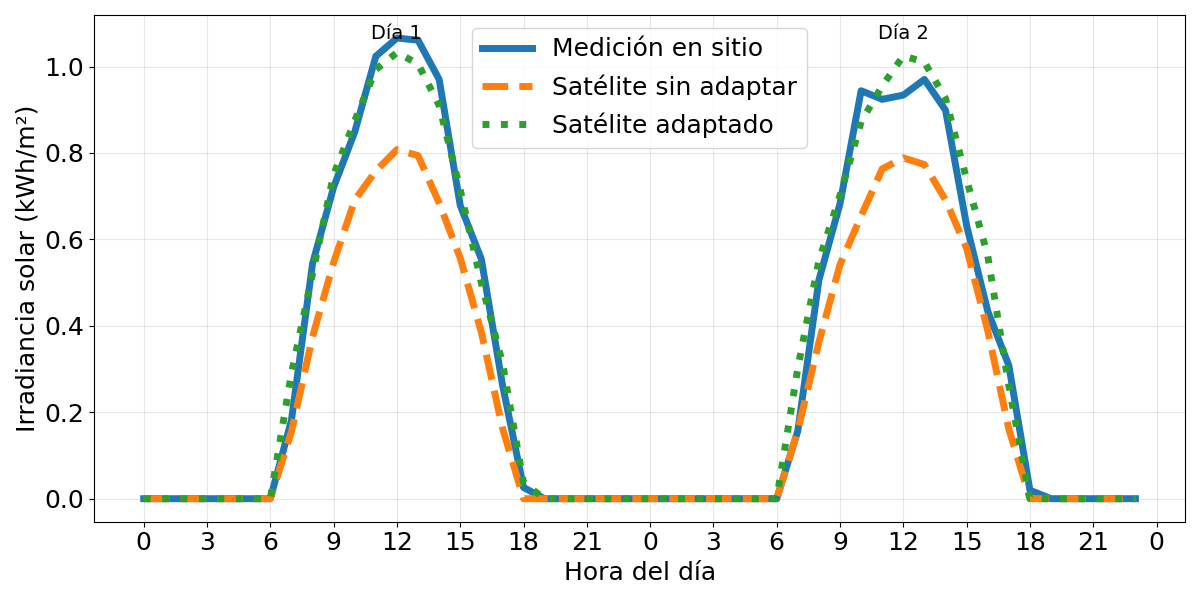
\includegraphics[width=0.97\linewidth]{figuras/SiteAdaptation-Example.png}
%DIFDELCMD <     \caption{Comparación de irradiancia solar diaria entre datos de satélite sin adaptar, datos de satélite adaptados y mediciones locales en el sitio de referencia. Se observa cómo la adaptación al sitio corrige el sesgo sistemático y mejora la representatividad de los datos satelitales.}
%DIFDELCMD <     \label{fig:example}
%DIFDELCMD < \end{figure}
%DIFDELCMD < 
%DIFDELCMD < 
%DIFDELCMD < La Figura \ref{fig:example}  ilustra una comparación entre tres conjuntos de datos de irradiancia solar a lo largo de dos días teóricos:
%DIFDELCMD < 
%DIFDELCMD < Medición en sitio (línea sólida): representa la referencia real tomada con instrumentos locales.
%DIFDELCMD < 
%DIFDELCMD < Modelada sin adaptar (línea discontinua): se observa un sesgo, ya que la serie está sistemáticamente desplazada respecto a la referencia. Además, los picos y valles no coinciden con exactitud, reflejando errores aleatorios.
%DIFDELCMD < 
%DIFDELCMD < Modelada adaptada (línea punteada): tras aplicar el procedimiento de adaptación al sitio, la serie corregida se ajusta mucho mejor a la referencia. El sesgo desaparece en gran medida y la forma de la curva sigue más de cerca la variabilidad de las mediciones locales.
%DIFDELCMD < 
%DIFDELCMD < Puede verse cómo la adaptación al sitio reduce tanto el error sistemático como la dispersión, logrando que los datos derivados de satélite sean más representativos de las condiciones reales de irradiancia en el lugar de interés.\\
%DIFDELCMD < 
%DIFDELCMD < 
%DIFDELCMD < En esencia, la Adaptación al Sitio se fundamenta en el principio de que los datos modelados por satélite o de re-análisis, aunque valiosos por su cobertura espacial y continuidad temporal, presentan inevitables limitaciones inherentes al proceso de observación remota. Estas limitaciones provienen de factores como la resolución espacial, los algoritmos de recuperación atmosférica, la presencia de nubosidad compleja o condiciones locales particulares que no son captadas por el modelo satelital.
%DIFDELCMD < 
%DIFDELCMD < Las mediciones terrestres, por el contrario, ofrecen alta precisión y captura directa de las condiciones atmosféricas locales, pero su disponibilidad está restringida en tiempo y espacio debido a los costos operativos de las estaciones de medición. La Adaptación al Sitio actúa, entonces, como un puente metodológico que buscar combinar las fortalezas de ambas fuentes de información, resultando en una serie híbrida que idealmente mantuviera precisión instrumental de las mediciones locales y la extensión temporal de los datos satelitales.
%DIFDELCMD < 
%DIFDELCMD < Técnicamente, los métodos empleados pueden abarcar desde procedimientos lineales sencillos —como la corrección por factores multiplicativos o aditivos— hasta técnicas avanzadas que incluyen regresión multivariante, modelos de error distribucional, aprendizaje automático y aproximaciones bayesianas. La selección del método adecuado depende del contexto del proyecto, la calidad y cantidad de datos disponibles, y el nivel de exactitud requerido.
%DIFDELCMD < 
%DIFDELCMD < Un aspecto central del proceso es la evaluación estadística previa y posterior a la corrección. Indicadores como sesgo medio (MBE) y el error cuadrático medio (RMSE) permiten cuantificar la magnitud de los errores iniciales y el grado de mejora logrado mediante la adaptación. Estas métricas buscan asegurar la trazabilidad y validez del procedimiento, lo cual es fundamental en aplicaciones energéticas y financieras.
%DIFDELCMD < 
%DIFDELCMD < La Adaptación al Sitio también implica la consideración de aspectos climáticos y estacionales. En regiones con alta variabilidad atmosférica o patrones climáticos complejos —por ejemplo, zonas montañosas, costeras o desérticas—, la calibración puede requerir tratamientos específicos para distintos regímenes de nubosidad o épocas del año. Esto asegura que las correcciones no solo reduzcan sesgos promedio, sino que también mejoren la representación de la variabilidad intra-anual del recurso solar.
%DIFDELCMD < 
%DIFDELCMD < Finalmente, la implementación de la Adaptación al Sitio contribuye directamente a la gestión del riesgo en proyectos renovables. Al minimizar la incertidumbre en la estimación del recurso solar, se fortalecen las bases técnicas para la toma de decisiones en financiamiento, operación y diseño energético, lo cual es especialmente relevante en mercados donde pequeños cambios en la previsión del recurso pueden significar diferencias significativas en los rendimientos económicos del proyecto.\\
%DIFDELCMD < 
%DIFDELCMD < 
%DIFDELCMD < \begin{figure}
%DIFDELCMD <     \centering
%DIFDELCMD <     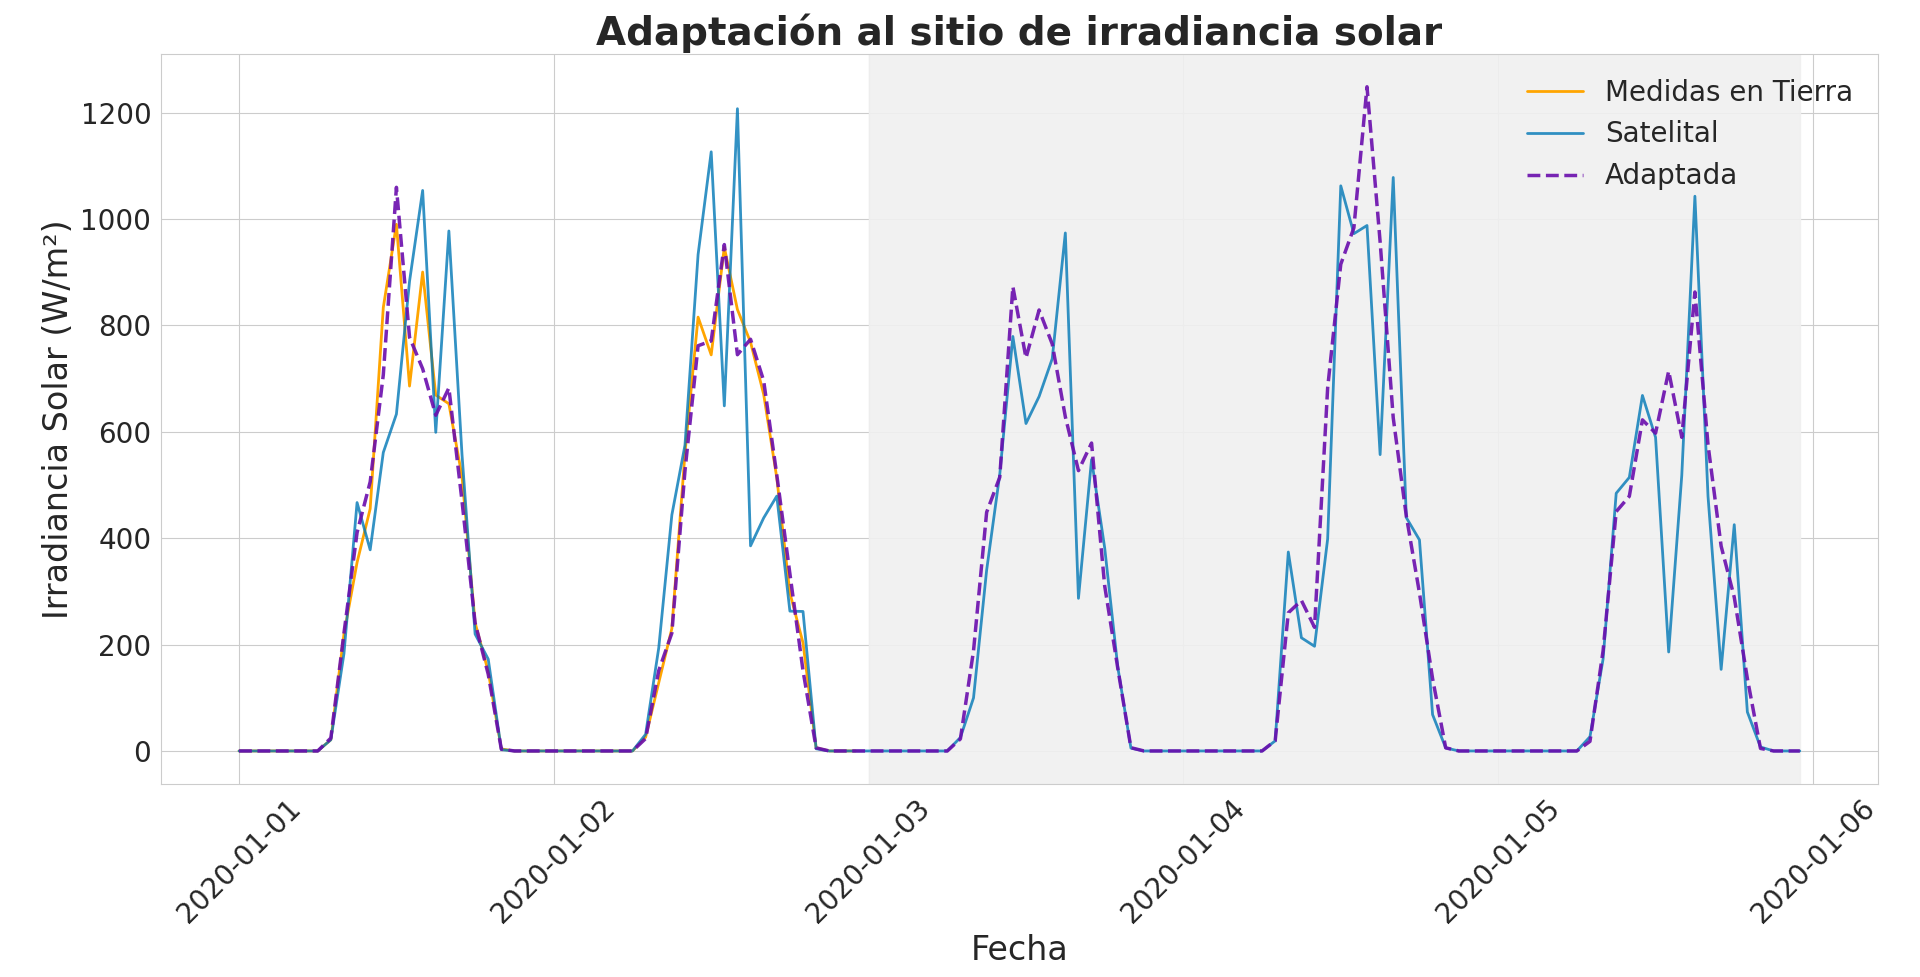
\includegraphics[width=0.97\linewidth]{figuras/siteAdaptation.png}
%DIFDELCMD <     \caption{Adaptación al Sitio sobre una serie genérica}
%DIFDELCMD <     \label{fig:site-adapation}
%DIFDELCMD < \end{figure}
%DIFDELCMD < 
%DIFDELCMD < En la Figura \ref{fig:site-adapation} puede verse el resultado que busca obtenerse al aplicar una adaptación al sitio. En color naranja se muestra la serie de medidas en tierra y en color azul la serie modelada, ambos casos con estilo de linea lleno. Debe tenerse en cuenta que el fondo cambiante de color (blanco y salmón) está realizado así a propósito.\\ 
%DIFDELCMD < \end{comment}
%DIFDELCMD < 

%DIFDELCMD < %%%
\DIFdel{Presentamos una analogía sencilla que ayude a explicar, de manera más cotidiana, la idea general del preceso de SA.
}%DIFDELCMD < \begin{quote}
%DIFDELCMD < %%%
\DIFdel{Pensemos en un agricultor de una zona rural que todos los días escucha por la radio el pronóstico de la temperatura. Esa información es fundamental para planificar su jornada: saber si debe llevar abrigo, más agua o proteger ciertos cultivos. En esta historia, ese pronóstico radial representa los datos de un modelo o de un satélite —una estimación general que sirve como guía, pero que no siempre refleja con precisión lo que ocurre en su propio terreno.
}%DIFDELCMD < 

%DIFDELCMD < %%%
\DIFdel{Después de notar que el pronóstico a menudo no coincide con la realidad local, el agricultor decide instalar un termómetro propio en su finca. De este modo, obtiene mediciones locales (análogas a las mediciones en sitio). Sin embargo, mantener ese sensor resulta costoso y difícil: la exposición al sol y la lluvia termina por dañarlo, por lo que solo logra registrar datos durante un período corto.
}%DIFDELCMD < 

%DIFDELCMD < %%%
\DIFdel{Al comparar esos registros con los pronósticos de la radio, descubre que su termómetro local siempre marca aproximadamente 5 °C menos en invierno y 3 ºC mas en verano que los valores reales promedio. Entonces aplica una corrección: suma 5 °C o resta 3 ºC a las predicciones del modelo según corresponda. A partir de ese ajuste, las estimaciones comienzan a representar mucho mejor las condiciones reales del lugar, incluso cuando el sensor ya no está disponible.
}%DIFDELCMD < 

%DIFDELCMD < %%%
\DIFdel{Eso, en esencia, es la Adaptación al Sitio: utilizar un período breve de mediciones reales como referencia para corregir los errores sistemáticos de los datos modelados o satelitales. Así, se logra que la información estimada sea más confiable y representativa del sitio específico —por ejemplo, para evaluar con mayor certeza el recurso solar de una futura planta fotovoltaica.
}%DIFDELCMD < \end{quote}
%DIFDELCMD < 

%DIFDELCMD < \begin{figure}
%DIFDELCMD < \centering
%DIFDELCMD < 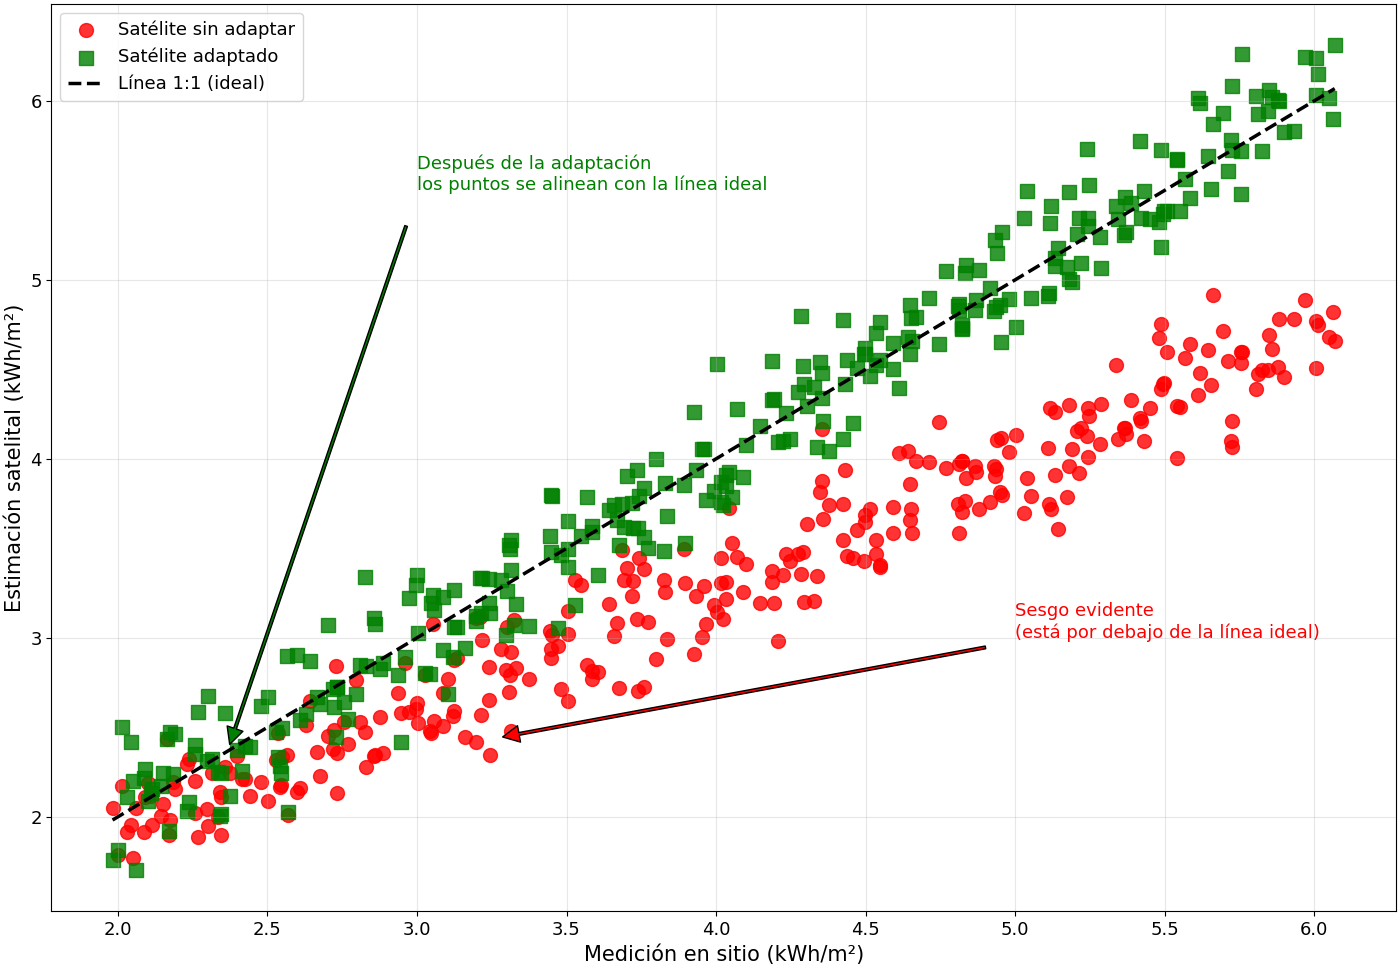
\includegraphics[width=\textwidth]{figuras/scatter-01.png}
%DIFDELCMD < %%%
%DIFDELCMD < \caption[Diagrama de dispersión entre mediciones en sitio y estimaciones satelitales.]{%
{%DIFAUXCMD
\DIFdelFL{Diagrama de dispersión entre mediciones en sitio y estimaciones satelitales.
Antes de la adaptación (puntos rojos), los datos muestran un sesgo claro al situarse por debajo de la línea 1:1. 
Después de la adaptación (puntos verdes), las estimaciones se alinean mucho mejor con la referencia, reduciendo el error sistemático.}}
%DIFAUXCMD
%DIFDELCMD < \label{fig:scatter01}
%DIFDELCMD < \end{figure}
%DIFDELCMD < 

%DIFDELCMD < %%%
\DIFdel{La Figura \ref{fig:scatter01} muestra de manera evidente el efecto de la adaptación al sitio:
}%DIFDELCMD < 

%DIFDELCMD < %%%
\DIFdel{Antes de la corrección (rojo): los puntos están sistemáticamente alejados de la línea 1:1, lo que indica que el satélite subestima los valores reales de irradiancia. Existe un sesgo claro.
}%DIFDELCMD < 

%DIFDELCMD < %%%
\DIFdel{Después de la corrección (verde): los puntos se agrupan alrededor de la línea 1:1, lo que significa que las estimaciones satelitales ahora representan con mayor fidelidad las mediciones en sitio.
}%DIFDELCMD < 

%DIFDELCMD < %%%
\section{\DIFdel{Estado del arte en Adaptación al Sitio}}
%DIFAUXCMD
\addtocounter{section}{-1}%DIFAUXCMD
\DIFdel{Al revisar la bibliografía sobre el proceso de adaptación al sitio frente a la radiación solar, se observa que esta técnica fue desarrollada en el siglo XXI y que su evolución ha sido rápida. Uno de los principales aportes sobre el tema fue realizado en el trabajo de \cite{POLO2016}, en el marco de la Tarea 46 del Programa de Calefacción y Refrigeración Solar de la Agencia Internacional de la Energía, Evaluación y pronóstico de recursos solares \citep{Task46}. En este trabajo se indica que la idea general de este proceso de corrección o calibración de datos modelados es similar a lo que se ha desarrollado en la industria eólica en el pasado \citep{Potter}.
}%DIFDELCMD < 

%DIFDELCMD < %%%
\DIFdel{Según Polo y sus colaboradores, el término Site Adaptation (SA) se emplea actualmente en proyectos de energía solar para describir la mejora que puede obtenerse en la irradiancia solar derivada de satélite y en los datos de modelos cuando se utilizan mediciones terrestres locales de corta duración para corregir sesgos y errores sistemáticos en los datos originales. A partir de esta definición general, Polo y su equipo proponen una clasificación de los métodos de SA en cinco categorías, que reúnen las principales estrategias destinadas a mejorar la precisión y reducir la incertidumbre de las estimaciones de radiación solar derivadas de satélite mediante el uso de mediciones locales de corta duración.
}%DIFDELCMD < 

%DIFDELCMD < %%%
\DIFdel{Durante la última década, la literatura ha consolidado cinco familias principales de métodos de SA:
}%DIFDELCMD < 

%DIFDELCMD < \begin{enumerate}
\begin{enumerate}%DIFAUXCMD
%DIFDELCMD <     \item %%%
\item%DIFAUXCMD
\DIFdel{\textbf{Métodos basados en modelos físicos (Physically based methods)}}%DIFDELCMD < \\
%DIFDELCMD <     %%%
\DIFdel{Este enfoque busca ajustar los datos de entrada atmosféricos (como la turbidez por aerosoles o el vapor de agua) de manera que los resultados del modelo coincidan mejor con las observaciones en tierra. Una evaluación de este enfoque fue realizada sobre el modelo REST2 \citep{Gueymard2008}, donde se buscó corregir la entrada del AOD (Aerosol Optical Depth), tal como se reporta en \citep{Gueymard2012}.
    }%DIFDELCMD < 

%DIFDELCMD <     \item %%%
\item%DIFAUXCMD
\DIFdel{\textbf{Métodos estadísticos (Statistical methods)}}%DIFDELCMD < \\
%DIFDELCMD <     %%%
\DIFdel{En diversos campos de la meteorología es común aplicar correcciones estadísticas sobre los datos modelados. Por ejemplo, las tasas de lluvia pueden corregirse para reflejar mejor las condiciones locales, o las velocidades del viento pueden adaptarse a mediciones locales para análisis de recursos eólicos. De manera similar, en este enfoque se ajustan los datos de un modelo con el objetivo de eliminar errores sistemáticos (sesgos) y mejorar la concordancia con los datos medidos localmente.}%DIFDELCMD < \\
%DIFDELCMD <     

%DIFDELCMD <     %%%
\DIFdel{Bajo este enfoque se han evaluado propuestas que buscan reducir el sesgo a partir de factores de corrección derivados de series medidas y modeladas superpuestas, como en \citep{Polo2015, Harmsen2014}, donde se aplican correcciones lineales sobre la serie modelada. También se han explorado alternativas no lineales que dependen de múltiples parámetros, utilizando funciones polinómicas \citep{Carow2008}.}%DIFDELCMD < \\
%DIFDELCMD <     

%DIFDELCMD <     %%%
\DIFdel{Dentro de este enfoque se incluyen los métodos basados en estadísticas de salida de modelos (Model Output Statistics, MOS) \citep{Bender2011}. MOS consiste en un análisis de regresión lineal multivariante entre un conjunto prescrito de predictores (por ejemplo, datos derivados de satélite o estimaciones de modelos de predicción meteorológica numérica) y observaciones de superficie. El objetivo es desarrollar una ecuación de regresión multilineal que corrija los valores estimados, eliminando el sesgo y ajustando la varianza.}%DIFDELCMD < \\
%DIFDELCMD <     

%DIFDELCMD <     %%%
\DIFdel{Además, dentro de este grupo se encuentran las denominadas \textit{Adaptaciones regionales}, que emplean estaciones cercanas. Estos métodos utilizan un período de superposición de datos derivados de terreno y modelo para desarrollar una corrección aplicable a todo el registro del modelo, incluso en períodos sin datos superpuestos. Por lo tanto, su aplicación requiere disponer de al menos 9 a 12 meses de datos simultáneos para capturar efectos estacionales. Durante este período de superposición ---denominado aquí como período de \textit{calibración}--- se ajustan los parámetros de la función de corrección mediante técnicas estadísticas. Sin embargo, la disminución de la autocorrelación temporal al aumentar el tiempo entre el período de calibración y los períodos de corrección (anteriores o posteriores) suele no considerarse, lo que puede resultar en sobrecorrecciones o subcorrecciones. Este aspecto es especialmente crítico para el DNI, cuya variabilidad interanual es mayor que la del GHI \citep{Lohmann2006}.}%DIFDELCMD < \\
%DIFDELCMD <     

%DIFDELCMD <     %%%
\DIFdel{Para ampliar la disponibilidad de mediciones, algunos autores han propuesto utilizar observaciones de irradiancia en una o más ubicaciones cercanas al sitio objetivo, siempre que se considere la estructura de covarianza espacial entre los datos modelados y las mediciones terrestres \citep{Ruiz2013}.}%DIFDELCMD < \\
%DIFDELCMD <     

%DIFDELCMD <     %%%
\DIFdel{Finalmente, dentro de este enfoque se incluye la \textit{Adaptación mediante funciones de distribución acumulativa (CDF)}. En este método se busca ajustar la función de distribución acumulativa de los datos derivados de satélite para que coincida con la de los datos de tierra \citep{Cebecauer2012}.
    }%DIFDELCMD < 

%DIFDELCMD <     \item %%%
\item%DIFAUXCMD
\DIFdel{\textbf{Adaptación de parámetros de entrada del modelo satelital}}%DIFDELCMD < \\
%DIFDELCMD <     %%%
\DIFdel{En este caso, se modifican directamente los parámetros de entrada del modelo (por ejemplo, el índice de claridad o los datos atmosféricos) en lugar de los resultados de irradiancia.
    }%DIFDELCMD < 

%DIFDELCMD <     \item %%%
\item%DIFAUXCMD
\DIFdel{\textbf{Técnicas MCP aplicadas a datos satelitales y de reanálisis}}%DIFDELCMD < \\
%DIFDELCMD <     %%%
\DIFdel{Se utilizan métodos de correlación-predicción, comunes en energía eólica, para extender los datos de corto plazo a largo plazo mediante el apoyo de modelos de reanálisis.
    }%DIFDELCMD < 

%DIFDELCMD <     \item %%%
\item%DIFAUXCMD
\DIFdel{\textbf{Combinación de datos satelitales con modelos meteorológicos numéricos (NWP por sus siglas en ingles)}}%DIFDELCMD < \\
%DIFDELCMD <     %%%
\DIFdel{Este enfoque mejora la precisión mediante técnicas de regresión no paramétrica, como los modelos aditivos generalizados (GAM), que combinan datos satelitales con salidas de modelos meteorológicos numéricos.
}
\end{enumerate}%DIFAUXCMD
%DIFDELCMD < \end{enumerate}
%DIFDELCMD < 

%DIFDELCMD < %%%
\DIFdel{A partir del año 2020 se comenzaron a publicar diversos trabajos sobre Adaptación al Sitio (SA). En \citep{POLO2020} se presentan los resultados de adaptaciones realizadas en diez estaciones a escala horaria, considerando ocho modelos satelitales y dos de re-análisis. En \citep{Fernández2020} se evaluaron los resultados de la adaptación al sitio utilizando regresiones lineales múltiples (MLR) y se combinaron estos resultados con un ajuste mediante mapeo de cuantiles (QM). Este enfoque de ensamble de modelos mostró una reducción promedio del 1,7\% en el sesgo relativo y del 3,3\% en la desviación cuadrática media relativa a escala horaria. El estudio también sugiere que un año de datos es suficiente para entrenar los modelos de ajuste.
}%DIFDELCMD < 

%DIFDELCMD < %%%
\DIFdel{En el trabajo de \citep{BABAR2020} se evaluó el desempeño del proceso de SA en los valores medios diarios del modelo satelital CLARA-A2 y del modelo de re-análisis ERA5. Para ello, se utilizó un modelo de Random Forest para la regresión, incorporando como predictores los valores de GHI modelados por CLARA-A2 y ERA5, sus respectivos índices de cielo despejado y el ángulo cenital solar medio. Los resultados demostraron una reducción de la desviación cuadrática media de 17,9 W/m² a 16,2 W/m² y una corrección completa del sesgo inicial de -1,5 W/m². La motivación para adoptar un modelo de regresión basado en aprendizaje automático surgió de la hipótesis de que este tipo de algoritmo podría aplicar funciones de regresión distintas a cada subconjunto del espacio de datos predictivos. Este trabajo es uno de los primeros en utilizar modelos de aprendizaje automático como Random Forest para determinar una función de ajuste que calibra las mediciones en tierra y puede aplicarse a series de largo plazo.
}%DIFDELCMD < 

%DIFDELCMD < %%%
\DIFdel{A partir del trabajo de Babar y colaboradores, se han publicado diversos estudios en los que se exploran modelos de aprendizaje automático como alternativa para determinar funciones de ajuste sobre series modeladas, ya sean satelitales o de re-análisis.
}%DIFDELCMD < 

%DIFDELCMD < %%%
\DIFdel{En \citep{NARVAEZ2021} se evaluó la adaptación al sitio en series horarias, explorando el uso de redes neuronales y los modelos Random Forest y AdaBoost. El rendimiento de estos modelos se evaluó en función de las métricas obtenidas en comparación con los ajustes realizados mediante QM y MLR, donde Random Forest logró una mejora aproximada del 38\% con respecto a QM y MLR.
}%DIFDELCMD < 

%DIFDELCMD < %%%
\DIFdel{En \citep{YANG2021} se presenta una alternativa denominada Adaptación al Sitio Probabilística, que aprovecha la disponibilidad de múltiples modelos de estimación simultáneamente. Este enfoque combina regresiones de cuantiles sobre múltiples modelos a la vez para mejorar la precisión de la adaptación al sitio.
}%DIFDELCMD < 

%DIFDELCMD < %%%
\DIFdel{En el trabajo de \citep{SALAMALIKIS2022}, se aplicó SA al modelo Heliosat-4 con una resolución horaria mediante el entrenamiento de diferentes modelos de regresión para condiciones de cielo despejado y nublado, considerando segmentos de datos basados en rangos de 15° del ángulo cenital solar. En este estudió se reportó  que el sesgo se redujo en un 50\% y la desviación cuadrática media disminuyó en un 3,8\% en comparación con las estimaciones sin SA. Los mejores resultados de este trabajo se obtuvieron utilizando modelos de regresión basados en árboles de decisión, en particular Random Forest. Además, una característica a destacar sobre este trabajo es que los autores han buscado eliminar la estacionalidad de la serie definiendo $\Delta_{GHI}$ como la diferencia entre la GHI medida y la GHI modelada. Esta variable se utiliza entonces como objetivo para los modelos de regresión, y la GHI adaptada se calcula como la suma del GHI modelada y $\Delta_{GHI}$. Puede considerarse que los autores en este trabajo han buscado quitar la }%DIFDELCMD < \enquote{\textit{estacionalidad}} %%%
\DIFdel{de la serie. Esta práctica es ampliamente conocida y estudiada en el área del análisis de series temporales, es recomendada y analizada en estudios como \citep{THORNTON2013, Claveria2015}.   
}%DIFDELCMD < 

%DIFDELCMD < %%%
\DIFdel{En \citep{ZAINALI2024} se evaluó un proceso de SA en tres sitios del norte de Europa utilizando diversos ajustes de mapeo de cuantiles y modelos de aprendizaje automático para ajustar los datos del modelo STRANG. Los hallazgos indican que los modelos de aprendizaje automático generalmente obtienen un rendimiento superior al de los métodos estadísticos, logrando una mejora de hasta el 9,2\% en la reducción del sesgo.
}%DIFDELCMD < 

%DIFDELCMD < %%%
\section{\DIFdel{Características, Ventajas y Desventajas de la SA}}
%DIFAUXCMD
\addtocounter{section}{-1}%DIFAUXCMD
%DIFDELCMD < 

%DIFDELCMD < %%%
\DIFdel{Entendiendo que SA se define como el proceso de corrección de las series de irradiancia solar modeladas (ya sean satelitales o de reanálisis) mediante un periodo corto de mediciones terrestres de alta calidad. Entre sus principales características se destacan:
}%DIFDELCMD < 

%DIFDELCMD < %%%
\subsection{\DIFdel{Características}}
%DIFAUXCMD
\addtocounter{subsection}{-1}%DIFAUXCMD
%DIFDELCMD < 

%DIFDELCMD < \begin{itemize}
\begin{itemize}%DIFAUXCMD
%DIFDELCMD < \item %%%
\item%DIFAUXCMD
\DIFdel{Corrige sesgos sistemáticos y errores aleatorios.
}%DIFDELCMD < \item %%%
\item%DIFAUXCMD
\DIFdel{Su desempeño depende en gran medida de las condiciones locales.
}%DIFDELCMD < \item  %%%
\item%DIFAUXCMD
\DIFdel{Aproximadamente 1 año de mediciones suele ser suficiente para entrenar modelos robustos.
}%DIFDELCMD < \item %%%
\item%DIFAUXCMD
\DIFdel{Puede aplicarse a productos satelitales o de reanálisis en múltiples escalas temporales.
}%DIFDELCMD < \item %%%
\item%DIFAUXCMD
\DIFdel{Existen herramientas abiertas que facilitan su implementación.
}
\end{itemize}%DIFAUXCMD
%DIFDELCMD < \end{itemize}
%DIFDELCMD < 

%DIFDELCMD < %%%
\subsection*{\DIFdel{Ventajas}}
%DIFAUXCMD
%DIFDELCMD < \begin{itemize}
\begin{itemize}%DIFAUXCMD
%DIFDELCMD < \item %%%
\item%DIFAUXCMD
\DIFdel{Reducción significativa del sesgo.
}%DIFDELCMD < \item %%%
\item%DIFAUXCMD
\DIFdel{Mejora consistente en las métricas estadísticas.
}%DIFDELCMD < \item %%%
\item%DIFAUXCMD
\DIFdel{Flexibilidad metodológica desde modelos simples hasta algoritmos avanzados.
}%DIFDELCMD < \item %%%
\item%DIFAUXCMD
\DIFdel{Útil en múltiples aplicaciones energéticas y climáticas.
}
\end{itemize}%DIFAUXCMD
%DIFDELCMD < \end{itemize}
%DIFDELCMD < 

%DIFDELCMD < %%%
\subsection*{\DIFdel{Desventajas y limitaciones}}
%DIFAUXCMD
%DIFDELCMD < 

%DIFDELCMD < \begin{itemize}
\begin{itemize}%DIFAUXCMD
%DIFDELCMD < \item %%%
\item%DIFAUXCMD
\DIFdel{Requiere datos locales de alta calidad.
}%DIFDELCMD < \item %%%
\item%DIFAUXCMD
\DIFdel{Alcance espacial limitado: la corrección es esencialmente local.
}%DIFDELCMD < \item %%%
\item%DIFAUXCMD
\DIFdel{No todos los métodos se generalizan entre regiones.
}%DIFDELCMD < \item %%%
\item%DIFAUXCMD
\DIFdel{Algunos modelos (especialmente los de ML) pueden requerir alta capacidad computacional.
}
\end{itemize}%DIFAUXCMD
%DIFDELCMD < \end{itemize}
%DIFDELCMD < 

%DIFDELCMD < %%%
\section{\DIFdel{Modelos de Aprendizaje Automático aplicados a SA}} %DIFAUXCMD
\addtocounter{section}{-1}%DIFAUXCMD
%DIFDELCMD < \label{MLM}
%DIFDELCMD < %%%
\DIFdel{Aunque Arthur Samuel no fue el primero en publicar un artículo que empleara el término ``aprendizaje automático'', se le atribuye la creación y definición de este concepto como el campo especializado que conocemos hoy. En su trabajo `Algunos estudios sobre aprendizaje automático usando el juego de damas' \cite{samuel1959}, presentó el aprendizaje automático como una rama de la informática que permite a las computadoras mejorar su desempeño sin necesidad de ser programadas de forma explícita.
}%DIFDELCMD < 

%DIFDELCMD < %%%
\DIFdel{Si bien la definición original de Samuel no lo menciona directamente, un aspecto fundamental del aprendizaje automático es el \textit{autoaprendizaje}. Este concepto implica el uso de modelos estadísticos para identificar patrones y optimizar el rendimiento con base en datos e información empírica, sin requerir instrucciones de programación explícitas \citep{Theobald2024}.
}%DIFDELCMD < 

%DIFDELCMD < \begin{comment}%DIFDELCMD < 
%DIFDELCMD < Samuel no infirió que las máquinas puedan tomar decisiones sin programación previa. Al contrario, el aprendizaje automático depende en gran medida de la entrada de código. En cambio, observó que las máquinas pueden realizar una tarea específica utilizando datos de entrada en lugar de depender de un comando de entrada directo.
%DIFDELCMD < 
%DIFDELCMD < \begin{figure}[H]
%DIFDELCMD <     \centering
%DIFDELCMD <     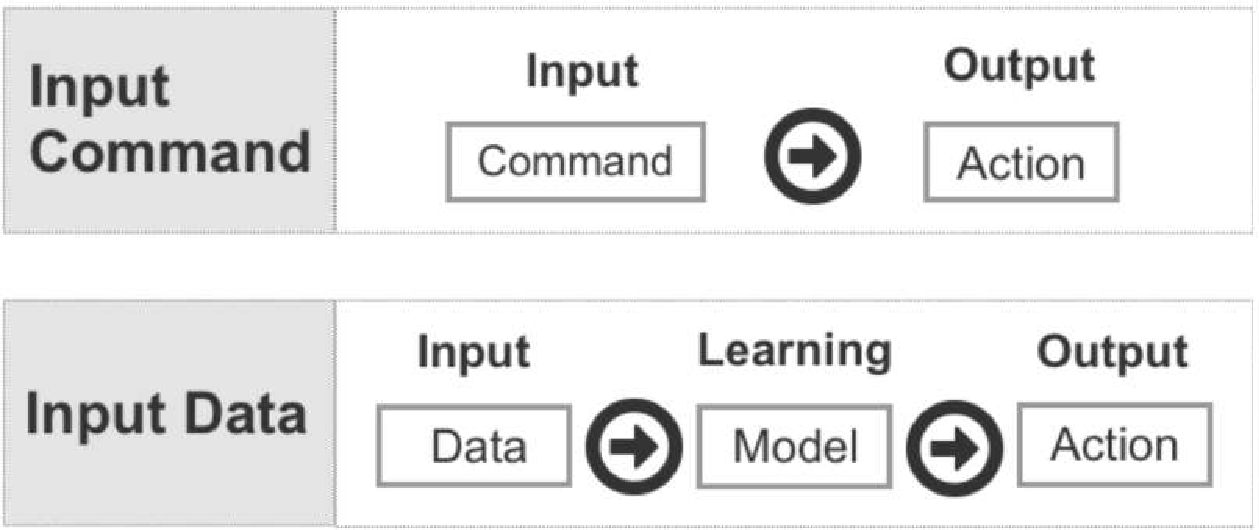
\includegraphics[scale=0.5]{figuras/ML.pdf}
%DIFDELCMD <     \caption{Comparación entre el comando de entrada y los datos de entrada}
%DIFDELCMD <     \label{fig:ML}
%DIFDELCMD < \end{figure}
%DIFDELCMD < \end{comment}
%DIFDELCMD < 

%DIFDELCMD <  \begin{comment}

\subsection{Modelo de red neuronal}

No existe una definición única de lo que es una red neuronal artificial, pero distintas fuentes proponen descripciones complementarias. Algunas de las más comunes son:

\begin{itemize}
    \item Un modelo computacional, paralelo, compuesto por unidades procesadoras adaptativas altamente interconectadas.
    \item Un sistema de procesamiento de la información que aplica principios inspirados en la organización del cerebro humano.
    \item Un modelo matemático diseñado para emular, de manera simplificada, el funcionamiento del cerebro.
    \item Un sistema de información con características de funcionamiento similares a las redes neuronales biológicas.
    \item Una red adaptativa que combina técnicas de procesamiento paralelo de la información.
    \item Una extensión de los métodos clásicos estadísticos, especialmente útil en el reconocimiento de patrones.
\end{itemize}

En todas estas definiciones se aprecia un componente de \textit{simulación biológica}. Las redes neuronales artificiales se inspiran en el cerebro humano en el sentido de que el procesamiento de la información se distribuye entre elementos básicos llamados \textit{neuronas}. Estas están interconectadas mediante \textit{pesos sinápticos}, que se ajustan a lo largo del tiempo durante un proceso denominado \textit{aprendizaje}. En términos simples, aprender consiste en modificar la intensidad de las conexiones entre neuronas para resolver una tarea determinada.

\subsubsection*{Neurona artificial}

Los componentes básicos de una neurona artificial son:

\begin{enumerate}
    \item Un conjunto de conexiones ponderadas (pesos sinápticos).
    \item Un sesgo, que actúa como umbral de activación.
    \item Un sumador, que agrega las entradas multiplicadas por sus pesos correspondientes.
    \item Una función de activación no lineal, que permite ampliar la capacidad de representación del modelo.
\end{enumerate}

\begin{figure}[H]
    \centering
    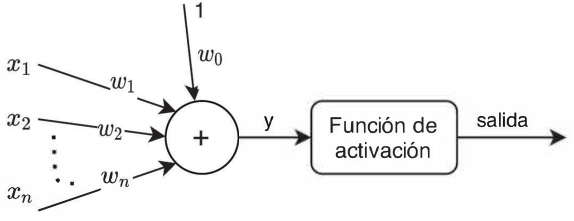
\includegraphics[scale=0.7]{figuras/neurona.png}
    \caption{Esquema de una neurona artificial}
    \label{fig:neurona}
\end{figure}

El funcionamiento matemático de una neurona artificial puede expresarse como:

\begin{equation}
    salida = f(y) = f\left( \sum_{k=0}^{n} w_{k}x_{k} \right)
    \label{eq:neurona}
\end{equation}

donde $x_i$ son las entradas, $w_i$ los pesos sinápticos y $x_0=1$ corresponde al sesgo con coeficiente $w_0$. La función $f$ representa la activación de la neurona.

\subsubsection*{Funciones de activación}

Las funciones de activación más comunes se resumen en la Tabla \ref{tab:activations}. Estas permiten introducir no linealidad en el modelo, lo cual es fundamental para que la red pueda aproximar funciones complejas.

\begin{table}[h]
    \centering
    \renewcommand{\arraystretch}{1.5}
    \begin{tabular}{|>{\centering\arraybackslash}p{2cm}|>{\centering\arraybackslash}p{5cm}|>{\centering\arraybackslash}p{8cm}|}
        \hline
        \textbf{Función} & \textbf{Expresión} & \textbf{Comentario} \\ 
        \hline
        Signo & 
        \( f(x) =
        \begin{cases} 
            1, & \text{si } x \geq 0 \\ 
            -1, & \text{si } x < 0 
        \end{cases} \)  
        & Usada en los primeros modelos de neuronas artificiales. \\ 
        \hline
        Sigmoide & 
        \( f(x) = \frac{1}{1 + e^{-x}} \)  
        & Transición suave entre 0 y 1, útil en clasificación binaria. \\ 
        \hline
        Tangente hiperbólica & 
        \( f(x) = \frac{e^x - e^{-x}}{e^x + e^{-x}} \)  
        & Similar a la sigmoide, pero con valores entre -1 y 1. \\ 
        \hline
        ReLU & 
        \( f(x) = \max(0, x) \)  
        & Una de las más usadas actualmente; evita problemas de gradiente. \\ 
        \hline
        Softmax & 
        \( f(x_i) = \frac{e^{x_i}}{ \sum_{k} e^{x_k} } \)  
        & Utilizada en la salida de modelos de clasificación multiclase. \\ 
        \hline
    \end{tabular}
    \caption{Funciones de activación más comunes en redes neuronales artificiales.}
    \label{tab:activations}
\end{table}

\subsubsection*{Perceptrón y sus limitaciones}

El perceptrón simple, basado en esta estructura, funciona como un clasificador binario que sólo puede resolver problemas linealmente separables. El procedimiento de aprendizaje consiste en:

\begin{enumerate}
    \item Inicializar aleatoriamente los pesos $w_{k}$.
    \item Establecer el parámetro de aprendizaje $\alpha$.
    \item Calcular la salida: $salida = signo(\sum_{k=0}^{n} w_{k} x_{k})$.
    \item Calcular el error: $error = salida_{deseada} - salida$.
    \item Actualizar los pesos: $w_{k} = w_{k} + \alpha \cdot error \cdot x_{k}$.
    \item Repetir el proceso.
\end{enumerate}

Aunque este modelo es simple y útil, su capacidad de representación es limitada. Para superar estas restricciones se introducen las redes \textbf{multicapa}.

\end{comment}
%DIFDELCMD < 

%DIFDELCMD < %%%
\subsubsection*{\DIFdel{Perceptrón Multicapa (MLP)}}
%DIFAUXCMD
%DIFDELCMD < 

%DIFDELCMD < %%%
\DIFdel{El \textit{Perceptrón Multicapa} (MLP, por sus siglas en inglés) organiza neuronas en diferentes capas: una capa de entrada, una o varias capas ocultas y una capa de salida (Fig. \ref{fig:MLP}). Gracias a esta estructura, el MLP puede aproximar funciones no lineales y resolver problemas más complejos.
}%DIFDELCMD < 

%DIFDELCMD < \begin{figure}
%DIFDELCMD <     \centering
%DIFDELCMD <     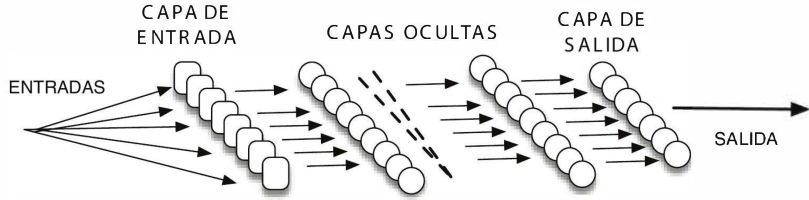
\includegraphics[scale=0.6]{figuras/MLP.png}
%DIFDELCMD <     %%%
%DIFDELCMD < \caption{%
{%DIFAUXCMD
\DIFdelFL{Esquema de una red neuronal multicapa (MLP).}}
    %DIFAUXCMD
%DIFDELCMD < \label{fig:MLP}
%DIFDELCMD < \end{figure}
%DIFDELCMD < \begin{comment}%DIFDELCMD < 
%DIFDELCMD < Un MLP con una capa oculta se puede definir como:
%DIFDELCMD < 
%DIFDELCMD < \begin{equation}
%DIFDELCMD < \hat{y} = f^{(2)}\Big( W^{(2)} \cdot f^{(1)}( W^{(1)} x + b^{(1)} ) + b^{(2)} \Big),
%DIFDELCMD < \end{equation}
%DIFDELCMD < 
%DIFDELCMD < donde $x$ es el vector de entrada, $W^{(1)}, W^{(2)}$ son matrices de pesos, $b^{(1)}, b^{(2)}$ los sesgos y $f^{(1)}, f^{(2)}$ las funciones de activación de cada capa \cite{ghanou2016mlp}.
%DIFDELCMD < \end{comment}
%DIFDELCMD < 

%DIFDELCMD < %%%
\DIFdel{En el contexto de la estimación de la GHI, el MLP puede verse como un \textit{equipo de expertos neuronales}. Cada neurona aporta una “opinión parcial” a partir de las variables meteorológicas (nubosidad, humedad, ángulo solar, aerosoles), mientras que las capas ocultas integran estas opiniones para refinar la predicción de manera no lineal \citep{torobayona2012mlp}.  
}%DIFDELCMD < 

%DIFDELCMD < \begin{figure} 
%DIFDELCMD < \centering 
%DIFDELCMD < \begin{tikzpicture}[node distance=2.2cm]
%DIFDELCMD < \tikzstyle{neuron} = [circle, draw, minimum size=1cm, fill=blue!20, text centered]
%DIFDELCMD < \tikzstyle{output} = [rectangle, draw, thick, rounded corners, text centered, minimum height=1cm, minimum width=3cm, fill=green!20]
%DIFDELCMD < 

%DIFDELCMD < \node (input1) [neuron] {Nubosidad};
%DIFDELCMD < \node (input2) [neuron, below of=input1] {Humedad};
%DIFDELCMD < \node (input3) [neuron, below of=input2] {Ángulo solar};
%DIFDELCMD < 

%DIFDELCMD < \node (hidden1) [neuron, right of=input1, xshift=4cm] {Oculta 1};
%DIFDELCMD < \node (hidden2) [neuron, below of=hidden1] {Oculta 2};
%DIFDELCMD < 

%DIFDELCMD < \node (final) [output, right of=hidden1, xshift=4cm, yshift=-1cm] {Predicción de GHI};
%DIFDELCMD < 

%DIFDELCMD < \foreach \i in {input1,input2,input3}{
%DIFDELCMD < \foreach \j in {hidden1,hidden2}{
%DIFDELCMD < \draw[flecha] (\i.east) -- (\j.west);
%DIFDELCMD < }
%DIFDELCMD < }
%DIFDELCMD < \foreach \j in {hidden1,hidden2}{
%DIFDELCMD < \draw[flecha] (\j.east) -- (final.west);
%DIFDELCMD < }
%DIFDELCMD < \end{tikzpicture}
%DIFDELCMD < %%%
%DIFDELCMD < \caption{%
{%DIFAUXCMD
\DIFdelFL{Analogía del MLP como un conjunto de expertos neuronales que refinan la predicción de la GHI.}}
%DIFAUXCMD
%DIFDELCMD < \label{fig:mlp_experts}
%DIFDELCMD < \end{figure}
%DIFDELCMD < 

%DIFDELCMD < %%%
\DIFdel{El MLP ofrece una estructura potente y flexible capaz de modelar relaciones no lineales complejas, esto permite considerarlo como una herramienta adecuada para la estimación de irradiancia solar.
}%DIFDELCMD < 

%DIFDELCMD < \begin{comment}%DIFDELCMD < 
%DIFDELCMD < 
%DIFDELCMD < \subsubsection*{Ejemplo práctico de entrenamiento en un MLP}
%DIFDELCMD < 
%DIFDELCMD < Para ilustrar el funcionamiento del \textit{Perceptrón Multicapa} (MLP), consideremos un ejemplo sencillo con dos entradas, una capa oculta con dos neuronas y una salida (Figura \ref{fig:mlp_ejemplo}).  
%DIFDELCMD < 
%DIFDELCMD < \begin{figure}[H]
%DIFDELCMD <     \centering
%DIFDELCMD <     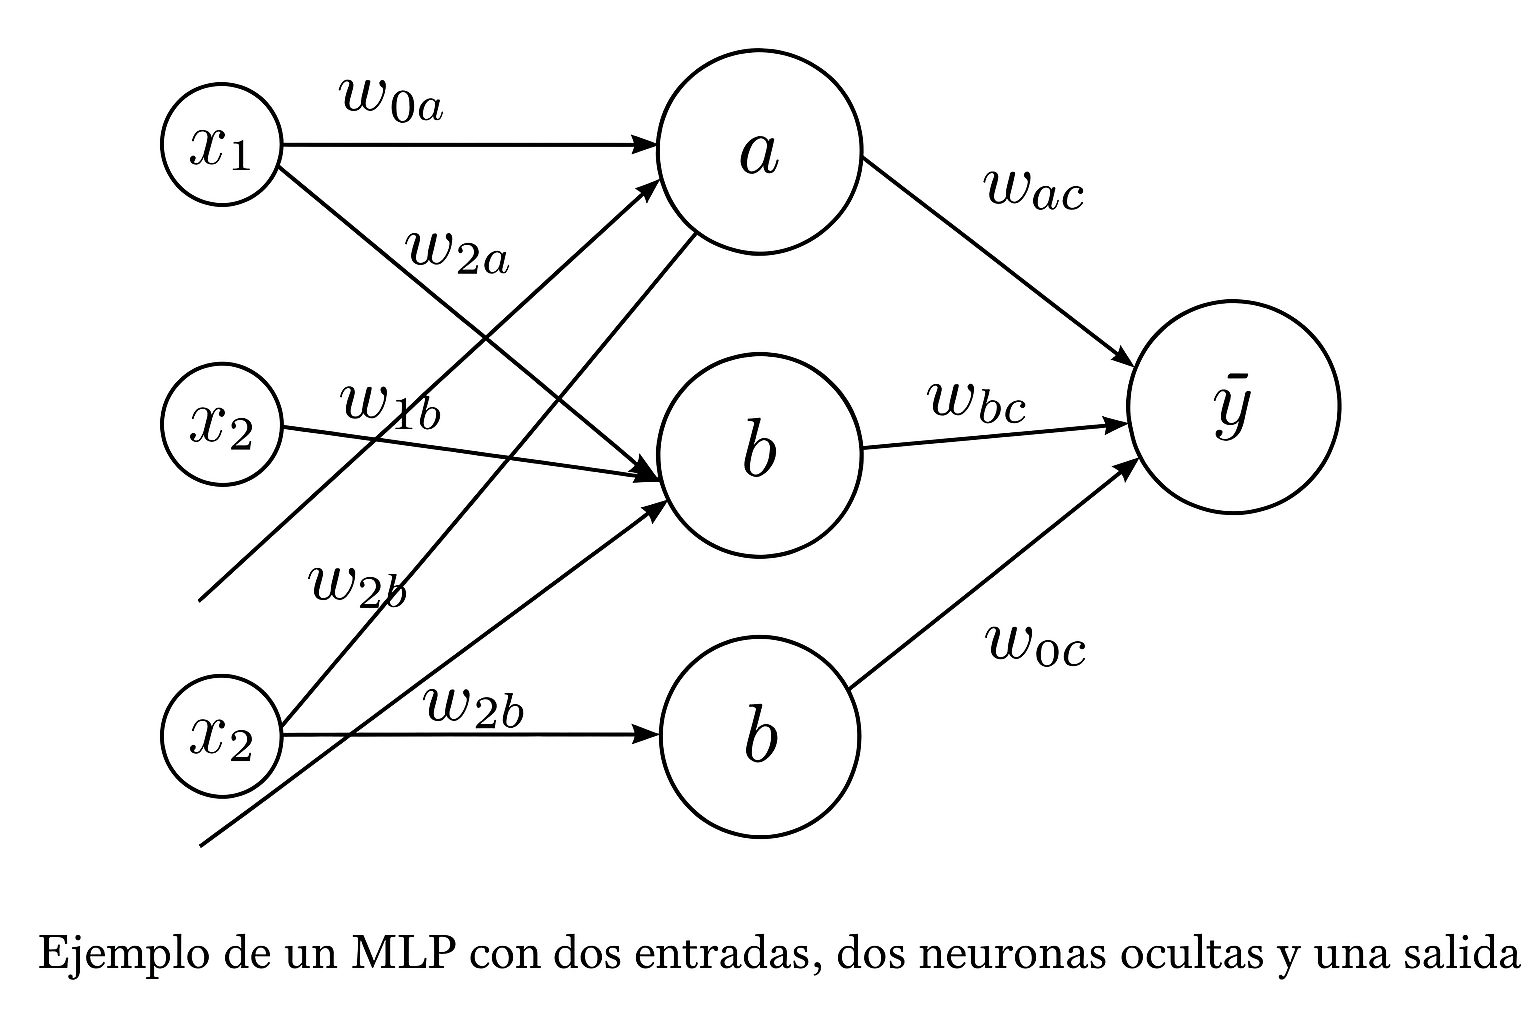
\includegraphics[scale=0.2]{figuras/mlp.png}
%DIFDELCMD <     \caption{Ejemplo de un MLP con dos entradas, dos neuronas ocultas y una salida.}
%DIFDELCMD <     \label{fig:mlp_ejemplo}
%DIFDELCMD < \end{figure}
%DIFDELCMD < 
%DIFDELCMD < 
%DIFDELCMD < 
%DIFDELCMD < 
%DIFDELCMD < 
%DIFDELCMD < El cálculo de las salidas se realiza en dos fases: propagación hacia adelante (\textit{forward pass}) y retropropagación del error (\textit{backpropagation}).
%DIFDELCMD < 
%DIFDELCMD < \paragraph{1. Propagación hacia adelante}
%DIFDELCMD < Las entradas $x_1$ y $x_2$ llegan a las dos neuronas ocultas $a$ y $b$:
%DIFDELCMD < 
%DIFDELCMD < \begin{equation}
%DIFDELCMD <     y_{a} = w_{0a} + w_{1a}x_{1} + w_{2a}x_{2}, \quad O_{a} = f(y_{a})
%DIFDELCMD < \end{equation}
%DIFDELCMD < \begin{equation}
%DIFDELCMD <     y_{b} = w_{0b} + w_{1b}x_{1} + w_{2b}x_{2}, \quad O_{b} = f(y_{b})
%DIFDELCMD < \end{equation}
%DIFDELCMD < 
%DIFDELCMD < Las salidas $O_{a}$ y $O_{b}$ alimentan a la neurona de salida $c$:
%DIFDELCMD < 
%DIFDELCMD < \begin{equation}
%DIFDELCMD <     y_{c} = w_{0c} + w_{ac}O_{a} + w_{bc}O_{b}, \quad \hat{y} = f(y_{c})
%DIFDELCMD < \end{equation}
%DIFDELCMD < 
%DIFDELCMD < donde $f(\cdot)$ es una función de activación diferenciable (sigmoide, tangente hiperbólica, ReLU, etc.).
%DIFDELCMD < 
%DIFDELCMD < \paragraph{2. Cálculo del error}
%DIFDELCMD < Dado un valor deseado $y$, el error cuadrático medio (ECM) para un ejemplo es:
%DIFDELCMD < 
%DIFDELCMD < \begin{equation}
%DIFDELCMD <     E = \frac{1}{2}(y - \hat{y})^2
%DIFDELCMD < \end{equation}
%DIFDELCMD < 
%DIFDELCMD < \paragraph{3. Retropropagación}
%DIFDELCMD < El objetivo es calcular cómo varía el error respecto a cada peso y ajustar estos valores en la dirección del gradiente descendente.
%DIFDELCMD < 
%DIFDELCMD < \begin{itemize}
%DIFDELCMD <     \item Para la salida $c$:
%DIFDELCMD <     \begin{equation}
%DIFDELCMD <         \delta_c = (y - \hat{y}) f'(y_{c})
%DIFDELCMD <     \end{equation}
%DIFDELCMD <     \item Para las neuronas ocultas $a$ y $b$:
%DIFDELCMD <     \begin{equation}
%DIFDELCMD <         \delta_a = f'(y_{a}) \cdot (w_{ac}\delta_c), \quad
%DIFDELCMD <         \delta_b = f'(y_{b}) \cdot (w_{bc}\delta_c)
%DIFDELCMD <     \end{equation}
%DIFDELCMD < \end{itemize}
%DIFDELCMD < 
%DIFDELCMD < \paragraph{4. Actualización de pesos}
%DIFDELCMD < Finalmente, los pesos se actualizan usando una tasa de aprendizaje $\eta$:
%DIFDELCMD < 
%DIFDELCMD < \begin{equation}
%DIFDELCMD <     w_{ij} \leftarrow w_{ij} + \eta \cdot \delta_j \cdot x_i
%DIFDELCMD < \end{equation}
%DIFDELCMD < 
%DIFDELCMD < donde $x_i$ es la entrada a la neurona $j$. Este procedimiento se repite para todos los ejemplos del conjunto de entrenamiento hasta que el error sea lo suficientemente pequeño.
%DIFDELCMD < 
%DIFDELCMD < \paragraph{5. Resumen del ciclo de aprendizaje}
%DIFDELCMD < \begin{enumerate}
%DIFDELCMD <     \item Inicializar pesos y sesgos aleatoriamente.
%DIFDELCMD <     \item Realizar la propagación hacia adelante para obtener la salida $\hat{y}$.
%DIFDELCMD <     \item Calcular el error $E$ comparando con el valor real $y$.
%DIFDELCMD <     \item Retropropagar el error para obtener los deltas $\delta$ de cada neurona.
%DIFDELCMD <     \item Actualizar los pesos usando la regla de gradiente descendente.
%DIFDELCMD <     \item Repetir el proceso hasta la convergencia.
%DIFDELCMD < \end{enumerate}
%DIFDELCMD < 
%DIFDELCMD < Este procedimiento es la base del entrenamiento de redes neuronales modernas. A pesar de su simplicidad, este esquema permite que los MLP aproximen relaciones altamente no lineales, siendo especialmente útiles para la estimación de la irradiancia solar, donde influyen múltiples variables meteorológicas de manera simultánea.
%DIFDELCMD < 
%DIFDELCMD < 
%DIFDELCMD < \end{comment}
%DIFDELCMD < 

%DIFDELCMD < %%%
\subsection{\DIFdel{Arboles de Decisión}}
%DIFAUXCMD
\addtocounter{subsection}{-1}%DIFAUXCMD
\DIFdel{Los árboles de decisión son modelos no paramétricos (es decir que no se no toman suposiciones previas sobre la forma de distribución de los datos) que se utilizan principalmente para la resolución de problemas de clasificación o regresión. También son conocidos como árboles de clasificación y regresión (CART, classification and regression trees). Este tipo de modelo fue propuesto por Leo Breiman en el libro \cite{breiman1984}.
}%DIFDELCMD < 

%DIFDELCMD < \begin{comment}%DIFDELCMD < 
%DIFDELCMD < Los árboles de decisión se basan en una serie de reglas de decisión para dividir el espacio de características predictoras en un número menor de regiones disjuntas en cada una de las cuales los valores de la variable respuesta son similares.
%DIFDELCMD < 
%DIFDELCMD < 
%DIFDELCMD < 
%DIFDELCMD < Los árboles de decisión se pueden clasificar en función del tipo de variable respuesta, si la variable de respuesta $y$ es cuantitativa el árbol es de regresión, si $y$ es cuantitativa el árbol es de clasificación.
%DIFDELCMD < 
%DIFDELCMD < \begin{figure}
%DIFDELCMD <     \centering
%DIFDELCMD <     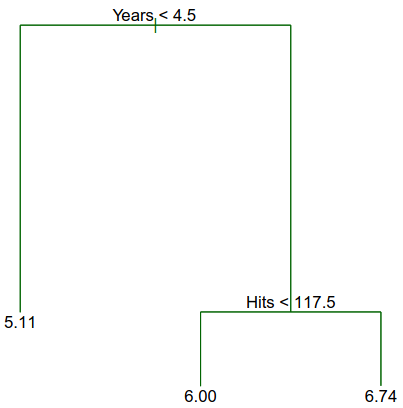
\includegraphics[width=0.25\linewidth]{figuras/tree_1.png}
%DIFDELCMD <     \caption{Ejemplo Árbol de Regresión. Para los datos de Hitters, se construye un árbol de regresión para predecir el logaritmo del salario de un jugador de béisbol, en función del número de años que ha jugado en las grandes ligas y el número de hits que realizó en el año anterior.}
%DIFDELCMD <     \label{fig:tree}
%DIFDELCMD < \end{figure}
%DIFDELCMD < 
%DIFDELCMD < 
%DIFDELCMD < El proceso general de construcción de un árbol de regresión puede describirse en dos pasos:
%DIFDELCMD < \begin{enumerate}
%DIFDELCMD <     \item  Dividir el espacio de predictores: es decir, el conjunto de valores posibles de $X_1, X_2, ..., X_p$ se divide en $J$ regiones distintas y no superpuestas, $R_1, R_2,..,R_J$.
%DIFDELCMD < 
%DIFDELCMD <     \item Hacer una predicción para cada región: para cada observación que cae en una región $R_j$, la predicción será simplemente la media de los valores de respuesta de las observaciones de entrenamiento dentro de $R_j$.
%DIFDELCMD < \end{enumerate}
%DIFDELCMD < \end{comment}
%DIFDELCMD < 

%DIFDELCMD < %%%
\subsection{\DIFdel{Random Forest}}
%DIFAUXCMD
\addtocounter{subsection}{-1}%DIFAUXCMD
\addcontentsline{toc}{subsection}{\DIFdel{Random Forest: Un Enfoque de Aprendizaje Autom\'atico}}
%DIFAUXCMD
%DIFDELCMD < 

%DIFDELCMD < %%%
\DIFdel{El algoritmo \textbf{Random Forest} (RF) es un modelo de aprendizaje supervisado de tipo \textit{ensemble} que se utiliza para resolver problemas de \textbf{clasificaci\'on} y \textbf{regresi\'on} \citep{louppe2015, salman2024}. Este m\'etodo, conceptualizado por Leo Breiman, es una extensi\'on del concepto de \textit{bagging} y se ha establecido como una t\'ecnica muy precisa y robusta en la miner\'ia de datos \citep{cutler2011}.
}%DIFDELCMD < 

%DIFDELCMD < %%%
\DIFdel{El fundamento de RF es la construcci\'on de un conjunto de m\'ultiples \'arboles de decisi\'on, donde cada \'arbol se entrena sobre un subconjunto de datos generado de forma aleatoria.
}%DIFDELCMD < 

%DIFDELCMD < \begin{comment}%DIFDELCMD < 
%DIFDELCMD < 
%DIFDELCMD < La aleatoriedad se introduce en dos niveles principales para garantizar que los \'arboles sean diversos y que el modelo no se sobreajuste:
%DIFDELCMD < 
%DIFDELCMD < \begin{enumerate}
%DIFDELCMD <     \item \textbf{Muestreo con reemplazo (Bootstrapping)}: Se generan m\'ultiples submuestras del conjunto de datos de entrenamiento original, con la posibilidad de que una misma observaci\'on aparezca varias veces en la misma submuestra. Cada submuestra se usa para entrenar un \'arbol de decisi\'on individual \cite{salman2024}.
%DIFDELCMD <     \item \textbf{Selecci\'on aleatoria de variables}: En cada nodo de un \'arbol, el algoritmo selecciona un subconjunto aleatorio de las variables predictoras disponibles. La mejor divisi\'on del nodo se determina a partir de este subconjunto reducido \cite{cutler2011, salman2024}. Esta t\'ecnica reduce la correlaci\'on entre los \'arboles y mejora la capacidad de generalizaci\'on del modelo \cite{cutler2011}.
%DIFDELCMD < \end{enumerate}
%DIFDELCMD < 
%DIFDELCMD < 
%DIFDELCMD < La divisi\'on \'optima en cada nodo del \'arbol se basa en la minimizaci\'on de una funci\'on de costo, que var\'ia seg\'un el tipo de problema.
%DIFDELCMD < 
%DIFDELCMD < Para problemas de \textbf{clasificaci\'on}, se utilizan medidas de impureza como el \textbf{\'indice Gini} o la \textbf{Entrop\'ia}. El \'Indice Gini mide la probabilidad de que una muestra elegida al azar de un nodo sea clasificada err\'oneamente, y se calcula de la siguiente manera:
%DIFDELCMD < $$
%DIFDELCMD < I_G(p) = 1 - \sum_{i=1}^{c} p_i^2
%DIFDELCMD < $$
%DIFDELCMD < donde $c$ es el n\'umero de clases y $p_i$ es la proporci\'on de muestras de la clase $i$ en el nodo.
%DIFDELCMD < 
%DIFDELCMD < Para problemas de \textbf{regresi\'on}, el criterio de divisi\'on se basa en la minimizaci\'on de la varianza o el \textbf{Error Cuadr\'atico Medio (MSE)} de las predicciones en los nodos hijos:
%DIFDELCMD < $$
%DIFDELCMD < MSE = \frac{1}{n} \sum_{i=1}^{n} (y_i - \hat{y}_i)^2
%DIFDELCMD < $$
%DIFDELCMD < donde $n$ es el n\'umero de muestras, $y_i$ es el valor real y $\hat{y}_i$ es el valor predicho.
%DIFDELCMD < 
%DIFDELCMD < Para realizar una predicci\'on final, el algoritmo agrega los resultados de todos los \'arboles del \textit{bosque} \cite{salman2024}. En problemas de \textbf{clasificaci\'on}, la predicci\'on se basa en el \textbf{voto mayoritario} de los \'arboles. Para problemas de \textbf{regresi\'on}, la predicci\'on final es el promedio de los resultados de cada \'arbol individual:
%DIFDELCMD < $$
%DIFDELCMD < \hat{y}_{RF}(\mathbf{x}) = \frac{1}{B} \sum_{b=1}^{B} h_b(\mathbf{x})
%DIFDELCMD < $$
%DIFDELCMD < donde $B$ es el n\'umero total de \'arboles en el bosque y $h_b(\mathbf{x})$ es la predicci\'on del $b$-\'esimo \'arbol.
%DIFDELCMD < 
%DIFDELCMD < 
%DIFDELCMD < Random Forest ofrece varias ventajas significativas para el an\'alisis de datos \cite{cutler2011}:
%DIFDELCMD < 
%DIFDELCMD < \begin{itemize}
%DIFDELCMD <     \item \textbf{Resistencia al sobreajuste (\textit{overfitting})}: El algoritmo es intr\'insecamente resistente al sobreajuste, ya que el conjunto de \'arboles se entrena en subconjuntos aleatorios de datos \cite{salman2024}.
%DIFDELCMD <     \item \textbf{Manejo de variables}: Es capaz de manejar eficientemente un gran n\'umero de variables, incluso cuando hay valores perdidos, sin necesidad de imputaci\'on previa \cite{cutler2011}.
%DIFDELCMD <     \item \textbf{Estimaci\'on de la importancia de las variables}: El algoritmo proporciona una medida integrada que indica la contribuci\'on relativa de cada variable al modelo, lo que facilita la interpretaci\'on de los resultados \cite{cutler2011}.
%DIFDELCMD < \end{itemize}
%DIFDELCMD < 
%DIFDELCMD < \end{comment}
%DIFDELCMD < 

%DIFDELCMD < %%%
\subsection{\DIFdel{XGBoost}}
%DIFAUXCMD
\addtocounter{subsection}{-1}%DIFAUXCMD
%DIFDELCMD < 

%DIFDELCMD < %%%
\DIFdel{El algoritmo \textit{Extreme Gradient Boosting} (XGBoost) es una implementación optimizada del método de \textit{Gradient Boosted Decision Trees} (GBDT) \citep{chen2016xgboost}.
Su funcionamiento consiste en combinar múltiples árboles de decisión simples para construir un modelo robusto, de manera semejante a cómo un equipo de especialistas aporta su conocimiento colectivo para tomar mejores decisiones.
XGBoost se ha consolidado como estado del arte en aprendizaje automático debido a su alto desempeño en tareas de clasificación y regresión en diversos dominios \citep{espinoza2020aplicacion}.}%DIFDELCMD < \\
%DIFDELCMD < 

%DIFDELCMD < %%%
\DIFdel{Para entender el algoritmo y su aplicación en la estimación de la GHI, podemos usar una analogía. Supongamos que deseamos predecir la GHI en un lugar específico.
}%DIFDELCMD < 

%DIFDELCMD < %%%
\DIFdel{Un único árbol de decisión actúa como un \textit{experto solitario}, que utiliza reglas simples para emitir un juicio, por ejemplo: \`si la nubosidad es alta, entonces la irradiancia será baja''. Aunque este razonamiento es útil, tiene limitaciones: la irradiancia también depende de la altura solar, aerosoles, humedad relativa o estacionalidad. Por ello, un solo árbol puede fallar al no capturar la complejidad completa del fenómeno.
}%DIFDELCMD < 

%DIFDELCMD < %%%
\DIFdel{XGBoost supera esta limitación mediante un \textit{comité de expertos}, es decir, un conjunto de árboles que se construyen secuencialmente para aprender de los errores de sus predecesores. Cada árbol nuevo se centra en corregir las predicciones incorrectas de los anteriores, especializándose en las regiones donde estos fallaron. Así, el modelo colectivo refina sus predicciones de manera progresiva. Esta dinámica se ilustra en la Figura \ref{fig:xgb_experts}.
}%DIFDELCMD < 

%DIFDELCMD < %%%
\DIFdel{Podemos compararlo con un proceso de deliberación científica: el primer investigador propone un modelo básico; otro detecta que no captura los días parcialmente nublados y lo corrige; un tercero ajusta los errores en días despejados con baja humedad. Con el tiempo, el grupo obtiene un modelo más completo que cualquiera de los expertos individuales.}%DIFDELCMD < \\
%DIFDELCMD < 

%DIFDELCMD < %%%
\DIFdel{Esta idea refleja la esencia del \textit{gradient boosting}: aprendizaje aditivo y secuencial, donde cada árbol se incorpora para reducir la pérdida residual del conjunto previo \cite{chen2016xgboost}. La fuerza del modelo final no está en la exactitud de cada árbol individual (clasificador débil), sino en la sinergia de todos ellos, formando un predictor colectivo altamente robusto.
En el caso de la estimación de GHI, el ensamble de árboles de XGBoost permite capturar relaciones complejas entre variables meteorológicas y solares, mientras controla el sobreajuste mediante regularización y técnicas adicionales como \textit{shrinkage} y submuestreo \cite{xgboostdoc}.
}%DIFDELCMD < 

%DIFDELCMD < %%%
\DIFdel{En resumen, si un árbol es un experto solitario con visión parcial, XGBoost funciona como un \textit{panel de expertos} que deliberan y corrigen mutuamente sus errores para alcanzar predicciones más precisas.
}%DIFDELCMD < 

%DIFDELCMD < \begin{figure} \centering \begin{tikzpicture}[node distance=2.2cm] % Estilos de nodos
%DIFDELCMD < \tikzstyle{expert} = [rectangle, draw, rounded corners, text centered, text width=3.5cm, minimum height=1cm, fill=blue!15] \tikzstyle{consensus} = [rectangle, draw, thick, rounded corners, text centered, text width=4.5cm, minimum height=1.2cm, fill=green!20] % Nodos de expertos 
%DIFDELCMD < \node (exp1) [expert] {Árbol 1:\\ Si nubosidad alta $\Rightarrow$ baja irradiancia''}; \node (exp2) [expert, below of=exp1] {Árbol 2:\\ Corrige error en días despejados}; \node (exp3) [expert, below of=exp2] {Árbol 3:\\ Ajusta casos con alta humedad}; \node (exp4) [expert, below of=exp3] {Árbol 4:\\ Mejora predicción en invierno}; % Nodo de consenso 
%DIFDELCMD < \node (final) [consensus, right of=exp2, xshift=8cm, yshift=-1cm] {Consenso del Comité (XGBoost):\\ Predicción refinada de GHI}; % Flechas de cada experto al consenso 
%DIFDELCMD < % Definir un estilo para las flechas \usetikzlibrary{decorations.markings} 
%DIFDELCMD < % cargar librería 
%DIFDELCMD < \tikzset{ flecha/.style={ thick, postaction={decorate, decoration={ markings, mark=at position 1 with {\arrow{>}} }} } } 
%DIFDELCMD < % Dibujar las flechas para los nodos exp1, exp2, exp3, exp4 hacia final
%DIFDELCMD < \foreach \i in {1,2,3,4}{ \draw[flecha] (exp\i.east) -- +(2,0) |- (final.west); } \end{tikzpicture} %%%
%DIFDELCMD < \caption[Analogía del comité de expertos en XGBoost.]{%
{%DIFAUXCMD
\DIFdelFL{Analogía del comité de expertos en XGBoost: cada árbol corrige los errores de sus predecesores y contribuye a una predicción final más precisa de la GHI.}} %DIFAUXCMD
%DIFDELCMD < \label{fig:xgb_experts} \end{figure}
%DIFDELCMD < 

%DIFDELCMD < \begin{comment}%DIFDELCMD < 
%DIFDELCMD < 
%DIFDELCMD < Formalmente, el modelo se define como:
%DIFDELCMD < 
%DIFDELCMD < \begin{equation}
%DIFDELCMD < \hat{y}_i = \sum_{k=1}^{K} f_k(x_i), \quad f_k \in \mathcal{F}, 
%DIFDELCMD < \end{equation}
%DIFDELCMD < 
%DIFDELCMD < donde cada $f_k$ es un árbol de regresión (\textit{CART}) y $\mathcal{F}$ es el espacio de todos los árboles posibles. La función objetivo combina el error de predicción y la complejidad del modelo:
%DIFDELCMD < 
%DIFDELCMD < \begin{equation}
%DIFDELCMD < \mathcal{L} = \sum_{i=1}^{n} l(y_i, \hat{y}_i) + \sum_{k=1}^{K} \Omega(f_k), 
%DIFDELCMD < \end{equation}
%DIFDELCMD < 
%DIFDELCMD < con regularización definida como:
%DIFDELCMD < 
%DIFDELCMD < \begin{equation} 
%DIFDELCMD < \Omega(f) = \gamma T + \frac{1}{2}\lambda \|w\|^2, 
%DIFDELCMD < \end{equation}
%DIFDELCMD < 
%DIFDELCMD < donde $T$ es el número de hojas, $w$ los pesos de cada hoja, $\gamma$ penaliza la complejidad del árbol y $\lambda$ regula la magnitud de los pesos \cite{chen2016xgboost}.
%DIFDELCMD < 
%DIFDELCMD < 
%DIFDELCMD < % Nuevo TikZ para árbol simple 
%DIFDELCMD < \begin{figure} 
%DIFDELCMD < \centering 
%DIFDELCMD < \begin{tikzpicture}[sibling distance=12em, every node/.style = {shape=rectangle, rounded corners, draw, align=center, top color=white, bottom color=blue!20}] 
%DIFDELCMD < \node {Nubosidad $<$ 50\%?} child { node {Sí \\ $\Rightarrow$ Alta irradiancia} } child { node {No \\ $\Rightarrow$ Baja irradiancia}};
%DIFDELCMD < \end{tikzpicture} 
%DIFDELCMD < \caption{Ejemplo de un árbol de decisión simple. XGBoost combina cientos de estos árboles débiles para construir un modelo poderoso.} 
%DIFDELCMD < \label{fig:treeexample} 
%DIFDELCMD < \end{figure}
%DIFDELCMD < 
%DIFDELCMD < XGBoost entrena los árboles de manera \textit{aditiva}, es decir, cada iteración añade un árbol que corrige los errores acumulados. Para ello utiliza una expansión de segundo orden de la función objetivo:
%DIFDELCMD < 
%DIFDELCMD < \begin{equation} 
%DIFDELCMD < \mathcal{L}^{(t)} \approx \sum_{i=1}^n \left[ g_i f_t(x_i) + \frac{1}{2} h_i f_t^2(x_i) \right] + \Omega(f_t), 
%DIFDELCMD < \end{equation}
%DIFDELCMD < 
%DIFDELCMD < donde $g_i$ y $h_i$ son el gradiente y la segunda derivada de la función de pérdida en la predicción previa. Esta formulación otorga estabilidad y precisión al proceso de entrenamiento \cite{chen2016xgboost}.
%DIFDELCMD < 
%DIFDELCMD < 
%DIFDELCMD < El proceso iterativo se representa en la Figura \ref{fig:boosting}.
%DIFDELCMD < 
%DIFDELCMD < % TikZ proceso iterativo 
%DIFDELCMD < \begin{figure} 
%DIFDELCMD < \centering 
%DIFDELCMD < \begin{tikzpicture}[node distance=2cm] % Nodos de iteración 
%DIFDELCMD < \node[rectangle, draw, fill=blue!20, rounded corners, minimum width=3cm, minimum height=1cm] (tree1) {Árbol 1: predicción inicial}; \node[rectangle, draw, fill=blue!20, rounded corners, minimum width=3cm, minimum height=1cm, below of=tree1] (tree2) {Árbol 2: corrige errores del árbol 1}; \node[rectangle, draw, fill=blue!20, rounded corners, minimum width=3cm, minimum height=1cm, below of=tree2] (tree3) {Árbol 3: corrige errores acumulados}; % Nodo de modelo final 
%DIFDELCMD < \node[rectangle, draw, fill=green!20, rounded corners, minimum width=4cm, minimum height=1cm, right of=tree2, xshift=6cm] (finalmodel) {Modelo XGBoost final}; 
%DIFDELCMD < % Flechas 
%DIFDELCMD < \foreach \i/\j in {tree1/finalmodel, tree2/finalmodel, tree3/finalmodel}{ \draw[flecha] (\i.east) -- (\j.west); } 
%DIFDELCMD < \end{tikzpicture} 
%DIFDELCMD < \caption{Proceso iterativo: cada nuevo árbol corrige los errores del modelo acumulado.} 
%DIFDELCMD < \label{fig:boosting} 
%DIFDELCMD < \end{figure}
%DIFDELCMD < 
%DIFDELCMD < 
%DIFDELCMD < XGBoost también incluye estrategias adicionales para mejorar la generalización \cite{xgboostdoc}:
%DIFDELCMD < 
%DIFDELCMD < \begin{itemize} 
%DIFDELCMD < \item \textbf{Shrinkage ($\eta$):} funciona como una `moderación'' en las decisiones del comité, reduciendo el impacto de cada nuevo árbol. 
%DIFDELCMD < \item \textbf{Submuestreo:} cada árbol se entrena con una muestra parcial de datos y características, como consultar a un subgrupo de expertos para ganar diversidad en las opiniones. 
%DIFDELCMD < \item \textbf{Regularización adicional:} actúa como una \textit{disciplina} que limita la complejidad de cada experto, evitando que se vuelva demasiado específico. 
%DIFDELCMD < \end{itemize}
%DIFDELCMD < 
%DIFDELCMD < En este estudio se utilizó la librería \texttt{xgboost} \cite{xgboostdoc}, con soporte para paralelización y GPU, lo que permitió un entrenamiento eficiente incluso con grandes volúmenes de datos. Los principales hiperparámetros (\texttt{max\_depth}, \texttt{eta}, \texttt{n\_rounds}, $\lambda$, $\gamma$) se ajustaron mediante \textit{grid search}.
%DIFDELCMD < 
%DIFDELCMD < De acuerdo a las especificaciones teóricas presentadas, consideramos que el uso de XGBoost es especialmente adecuado para el análisis de irradiancia solar porque:
%DIFDELCMD < 
%DIFDELCMD < \begin{enumerate}
%DIFDELCMD < \item Captura relaciones no lineales entre variables atmosféricas y solares.
%DIFDELCMD < \item Reduce el sobreajuste mediante mecanismos internos de regularización.
%DIFDELCMD < \item Permite escalabilidad y eficiencia en grandes bases de datos.
%DIFDELCMD < \item Suele superar a otros ensambles como Random Forest \cite{espinoza2020aplicacion}.
%DIFDELCMD < \end{enumerate}
%DIFDELCMD < 
%DIFDELCMD < % TikZ esquema conceptual 
%DIFDELCMD < \begin{figure} 
%DIFDELCMD < \centering 
%DIFDELCMD < \begin{tikzpicture}[node distance=1.5cm] \node[rectangle, draw, fill=blue!20, rounded corners, minimum width=3cm, minimum height=0.8cm] (t1) {Árbol 1}; \node[rectangle, draw, fill=blue!20, rounded corners, minimum width=3cm, minimum height=0.8cm, below of=t1] (t2) {Árbol 2}; \node[rectangle, draw, fill=blue!20, rounded corners, minimum width=3cm, minimum height=0.8cm, below of=t2] (t3) {Árbol 3}; \node[rectangle, draw, fill=green!20, rounded corners, minimum width=4cm, minimum height=1cm, right of=t2, xshift=6cm] (final) {Predicción colectiva XGBoost}; \foreach \i in {t1,t2,t3}{ \draw[flecha] (\i.east) -- +(2,0) |- (final.west); } \end{tikzpicture} \caption{Esquema conceptual: múltiples árboles (\textit{expertos}) corrigen iterativamente sus errores para formar un modelo robusto.} \label{fig:esquemaxgb} \end{figure}
%DIFDELCMD < 
%DIFDELCMD < 
%DIFDELCMD < La Figura \ref{fig:esquemaxgb} resumen la idea para una predicción generica utilizando XGBoost como modelo regresor.
%DIFDELCMD < 
%DIFDELCMD < 
%DIFDELCMD < En resumen, mientras que un árbol de decisión actúa como un experto solitario y XGBoost combina múltiples árboles secuencialmente, un MLP funciona como un sistema de neuronas interconectadas que colectivamente aprenden patrones complejos en los datos, logrando predicciones precisas de irradiancia solar.
%DIFDELCMD < \end{comment}
%DIFDELCMD < 

%DIFDELCMD < %%%
\section{\DIFdel{Entrenamiento, Validación y  Prueba}}
%DIFAUXCMD
\addtocounter{section}{-1}%DIFAUXCMD
%DIFDELCMD < 

%DIFDELCMD < %%%
\DIFdel{El proceso de construcción de un modelo de aprendizaje automático no termina en su diseño, sino que requiere fases diferenciadas de \textbf{entrenamiento}, \textbf{validación} y \textbf{prueba}, cuyo objetivo principal es garantizar la capacidad de generalización del modelo ante datos no observados. La correcta separación de los datos en entrenamiento, validación y prueba es esencial para evaluar la capacidad de generalización del modelo y evitar el sobreajuste.
}%DIFDELCMD < 

%DIFDELCMD < %%%
\subsection*{\DIFdel{División del conjunto de datos}}
%DIFAUXCMD
\DIFdel{La práctica estándar consiste en dividir el conjunto de datos en tres subconjuntos:
}%DIFDELCMD < 

%DIFDELCMD < \begin{itemize}
\begin{itemize}%DIFAUXCMD
%DIFDELCMD < \item %%%
\item%DIFAUXCMD
\DIFdel{\textbf{Entrenamiento}: utilizado para ajustar los parámetros internos del modelo (pesos y sesgos en redes neuronales, divisiones en árboles de decisión, etc.).
}%DIFDELCMD < \item %%%
\item%DIFAUXCMD
\DIFdel{\textbf{Validación}: empleado durante el entrenamiento para seleccionar hiperparámetros y evitar el sobreajuste (\textit{overfitting}). Una proporción habitual es 80\% para entrenamiento y 20\% para validación dentro del subconjunto inicial de entrenamiento.
}%DIFDELCMD < \item %%%
\item%DIFAUXCMD
\DIFdel{\textbf{Prueba (test)}: reservado exclusivamente para la evaluación final. Nunca se utiliza en la fase de ajuste, ya que su propósito es ofrecer una estimación imparcial del error de generalización.
}
\end{itemize}%DIFAUXCMD
%DIFDELCMD < \end{itemize}
%DIFDELCMD < 

%DIFDELCMD < %%%
\subsection*{\DIFdel{Dinámica de entrenamiento}}
%DIFAUXCMD
\DIFdel{Durante el entrenamiento, el error de entrenamiento disminuye progresivamente a medida que el modelo se ajusta a los datos. Paralelamente, el error de validación suele descender inicialmente, reflejando la mejora de la capacidad de generalización, hasta que alcanza un punto mínimo. A partir de ahí, si el entrenamiento continúa, el error de validación aumenta, lo que indica que el modelo comienza a memorizar los datos y pierde capacidad predictiva. Este fenómeno se conoce como \textbf{sobreajuste}, y la estrategia recomendada es detener el entrenamiento en el punto donde el error de validación es mínimo, aplicando técnicas como \textit{early stopping} o el almacenamiento de los mejores pesos (\textit{model checkpointing}).
}%DIFDELCMD < 

%DIFDELCMD < \begin{figure}
%DIFDELCMD <     \centering
%DIFDELCMD <     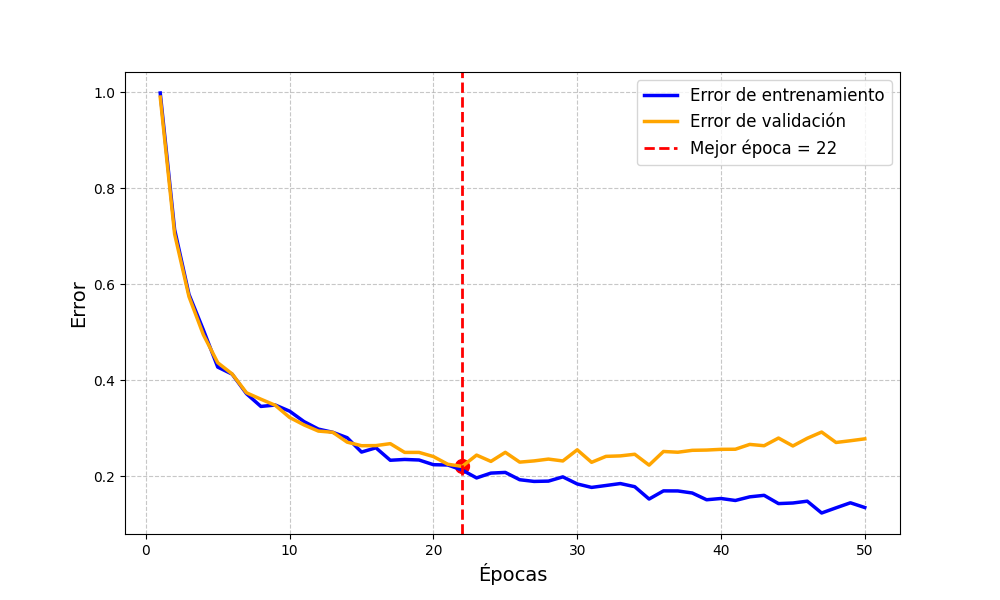
\includegraphics[scale=0.6]{figuras/dinamicatv.png}
%DIFDELCMD <     %%%
%DIFDELCMD < \caption[Dinámica de entrenamiento de un modelo de aprendizaje automático.]{%
{%DIFAUXCMD
\DIFdelFL{Dinámica de entrenamiento de un modelo de aprendizaje automático. La curva azul muestra el error de entrenamiento, que disminuye progresivamente a medida que el modelo se ajusta a los datos. La curva naranja representa el error de validación, que disminuye inicialmente reflejando la mejora de la capacidad de generalización, pero comienza a aumentar después de la mejor época (línea roja discontinua), evidenciando el sobreajuste.}}
    %DIFAUXCMD
%DIFDELCMD < \label{fig:dinamica}
%DIFDELCMD <     

%DIFDELCMD < \end{figure}
%DIFDELCMD < 

%DIFDELCMD < %%%
\DIFdel{La figura \ref{fig:dinamica} ilustra la dinámica durante el entrenamiento, indicando que el modelo se adapta cada vez mejor a los datos de entrenamiento. Por otro lado, el error de validación inicialmente sigue la misma tendencia, mostrando que la capacidad de generalización del modelo mejora. Sin embargo, después de alcanzar un punto mínimo —marcado como la mejor época en la figura—, el error de validación comienza a incrementarse, mientras que el error de entrenamiento sigue descendiendo. Este comportamiento refleja el fenómeno de \textbf{sobreajuste}, en el cual el modelo comienza a memorizar los datos de entrenamiento y pierde capacidad predictiva en datos nuevos. La figura ilustra claramente este efecto y destaca la importancia de detener el entrenamiento en la época óptima o emplear técnicas como \textit{early stopping} para evitar la degradación del desempeño en validación.
}%DIFDELCMD < 

%DIFDELCMD < \begin{comment}%DIFDELCMD < 
%DIFDELCMD < 
%DIFDELCMD < \subsection*{Técnicas de regularización y validación}
%DIFDELCMD < Para mejorar la robustez del modelo se emplean diversas estrategias:
%DIFDELCMD < 
%DIFDELCMD < \begin{itemize}
%DIFDELCMD < \item \textbf{Regularización}: penalizaciones sobre los parámetros (L1, L2) o el uso de \textit{dropout} en redes neuronales.
%DIFDELCMD < \item \textbf{Aumento de datos (Data Augmentation)}: generación de variaciones sintéticas del conjunto de entrenamiento para mejorar la capacidad de generalización.
%DIFDELCMD < \item \textbf{Validación cruzada (Cross-Validation)}: división repetida del conjunto de datos en diferentes particiones de entrenamiento y validación, promediando los resultados para obtener una estimación más estable.
%DIFDELCMD < \end{itemize}
%DIFDELCMD < \end{comment}
%DIFDELCMD < 

%DIFDELCMD < %%%
\subsection*{\DIFdel{Evaluación}}
%DIFAUXCMD
%DIFDELCMD < 

%DIFDELCMD < %%%
\DIFdel{Las métricas más relevantes en SA incluyen \textbf{MBE} (Error Medio de Sesgo), 
\textbf{MAE} (Error Medio Absoluto) y \textbf{RMSE} (Error Cuadrático Medio), 
así como sus versiones normalizadas \textbf{rMBE}, \textbf{rMAE} y \textbf{rRMSE},que permiten evaluar tanto el sesgo como la dispersión del error.
}%DIFDELCMD < 

%DIFDELCMD < %%%
\DIFdel{El MAE cuantifica el error medio absoluto entre valores observados y estimados, 
proporcionando una medida directa de la magnitud promedio de los errores sin considerar su signo. El RMSE penaliza en mayor medida los errores grandes, siendo particularmente sensible a discrepancias puntuales o valores atípicos. El MBE expresa el sesgo medio, indicando si el modelo sobreestima o subestima de forma sistemática; sus versiones relativas (rMBE, rMAE, rRMSE) expresan estas métricas como porcentajes del valor promedio medido, facilitando la comparación entre sitios con magnitudes de irradiancia distintas. En conjunto, estas métricas permiten evaluar la fidelidad del ajuste, las desviaciones sistemáticas y la consistencia del modelo en diferentes condiciones de operación.
}%DIFDELCMD < 

%DIFDELCMD < %%%
\section{\DIFdel{Síntesis del Capítulo}}
%DIFAUXCMD
\addtocounter{section}{-1}%DIFAUXCMD
\DIFdel{Este capítulo estableció los fundamentos teóricos de la Adaptación al Sitio, revisó los métodos disponibles en la literatura, describió los modelos de ML aplicados en esta tesis y presentó las bases del proceso de entrenamiento y evaluación. Este marco conceptual sostiene la metodología desarrollada en los capítulos siguientes.
}%DIFDELCMD < 

%DIFDELCMD <  \newpage  %%%
\DIFdelend \DIFaddbegin \include{Capitulo2} \DIFaddend %Obligatorio
\DIFdelbegin %DIFDELCMD < \newpage \lhead{Capítulo \ref{ch_3}}
%DIFDELCMD < %%%
%DIF < \rhead{\newtitle}
%DIFDELCMD < \rhead{}
%DIFDELCMD < \cfoot{\thepage}
%DIFDELCMD < \renewcommand{\headrulewidth}{1pt}
%DIFDELCMD < \renewcommand{\footrulewidth}{1pt}
%DIFDELCMD < %%%
\chapter{\DIFdel{Adaptación al Sitio en NOA}}%DIFAUXCMD
\addtocounter{chapter}{-1}%DIFAUXCMD
%DIFDELCMD < \label{ch_3}
%DIFDELCMD < 

%DIFDELCMD < %%%
\DIFdel{En este capítulo se aborda la aplicación de los métodos de adaptación al sitio en la región del Noroeste Argentino (NOA), con el objetivo de mejorar la representatividad espacial de las estimaciones de radiación solar provenientes de modelos satelitales y de reanálisis. A partir de las mediciones de GHI realizadas en distintas estaciones de Salta y Jujuy, se analiza el desempeño de los productos disponibles y se propone su corrección mediante técnicas de aprendizaje automático.
}%DIFDELCMD < 

%DIFDELCMD < %%%
\DIFdel{El desarrollo de este capítulo permite comprender cómo las particularidades geográficas y climáticas del NOA —su topografía compleja, la marcada variabilidad estacional y la diversidad de condiciones atmosféricas— influyen en la precisión de las estimaciones del recurso solar. Por ello, la adaptación al sitio se presenta no solo como una etapa metodológica, sino como una herramienta clave para trasladar los modelos globales a contextos locales, reduciendo sesgos y aumentando la confiabilidad de los datos.
}%DIFDELCMD < 

%DIFDELCMD < %%%
\DIFdel{A lo largo del capítulo se describen las estaciones de medida utilizadas, los procedimientos de control de calidad aplicados a las mediciones en tierra, las métricas empleadas para evaluar los modelos y los distintos enfoques de adaptación implementados, desde los más simples —con una variable descriptiva— hasta los más complejos, basados en múltiples regresores y en el aprovechamiento de información satelital adyacente. Finalmente, se discuten los resultados obtenidos, destacando las mejoras alcanzadas en la precisión y estabilidad de las estimaciones adaptadas, así como su potencial de generalización hacia otras zonas del NOA con condiciones similares.
}%DIFDELCMD < 

%DIFDELCMD < %%%
\section{\DIFdel{Medidas en superficie}}
%DIFAUXCMD
\addtocounter{section}{-1}%DIFAUXCMD
%DIFDELCMD < 

%DIFDELCMD < %%%
\DIFdel{Los sitios analizados en esta tesis se resumen en la Tabla \ref{tab:sites}, donde se incluyen sus códigos de identificación, coordenadas geográficas, altitud sobre el nivel del mar y su clasificación climática según Köppen–Geiger \citep{peel2007}. Estas estaciones  están ubicadas en el noroeste de Argentina como puede verse en la Figura \ref{fig:sites} y abarcan diversas condiciones climáticas y geográficas, que van desde tierras bajas subtropicales hasta altiplanos andinos de gran altitud.
}%DIFDELCMD < 

%DIFDELCMD < \begin{figure}
%DIFDELCMD <    \centering
%DIFDELCMD <    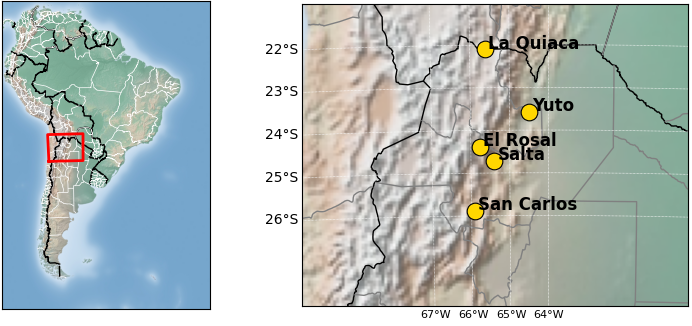
\includegraphics[width=1\linewidth]{figuras/sites.png}
%DIFDELCMD <     %%%
%DIFDELCMD < \caption{%
{%DIFAUXCMD
\DIFdelFL{Ubicación de la estaciones de medida.}}
    %DIFAUXCMD
%DIFDELCMD < \label{fig:sites}
%DIFDELCMD < \end{figure}
%DIFDELCMD < 

%DIFDELCMD < %%%
\DIFdel{La estación \textbf{Sa} (Salta Capital) se encuentra en el campus experimental del INENCO, en la Universidad Nacional de Salta. Está situada en un entorno urbano preandino dentro del Valle de Lerma, una zona donde es común la formación de nubes debido a la cercanía de la cordillera. Su clima es subtropical de montaña, con inviernos secos y veranos frescos (Cwb). Las mediciones se realizaron entre 2009 y 2020 utilizando un piranómetro Eppley PSP.
}%DIFDELCMD < 

%DIFDELCMD < %%%
\DIFdel{La estación \textbf{Lq} (Ciudad de La Quiaca - Jujuy), se encuentra ubicada en una región que un clima estepario frío semiárido (BSk) típico de regiones andinas, y destaca por registrar uno de los mayores niveles de horas de sol anuales en Argentina. Los datos fueron registrados mediante un piranómetro Kipp \& Zonen CMP11 entre los años 2018 y 2023.
}%DIFDELCMD < 

%DIFDELCMD < %%%
\DIFdel{La estación \textbf{Yu}, ubicada en una zona de clima subtropical húmedo (Cwa), registró datos entre 2017 y 2018 con un sensor CMP11. La estación \textbf{Sca}, también con clima Cwb, operó entre 2012 y 2013 con un piranómetro CMP3.	 Finalmente, la estación \textbf{Ero}, situada en una región de gran altitud con clima BSk, recopiló datos entre 2016 y 2018, igualmente con un CMP3.
}%DIFDELCMD < 

%DIFDELCMD < %%%
\DIFdel{Todas las estaciones utilizan piranómetros que cumplen con los estándares de la norma ISO 9060:2018 Clase A o B para la medición de la irradiancia global horizontal (GHI). Los datos se registraron a intervalos de un minuto, y cada valor corresponde al promedio de seis muestras tomadas cada 10 segundos.
}%DIFDELCMD < 

%DIFDELCMD < \begin{table}
%DIFDELCMD <     \centering
%DIFDELCMD <     \renewcommand{\arraystretch}{1.5} %%%
%DIF <  Espaciado vertical en la tabla
    %DIFDELCMD < \begin{tabular}{|>{\centering\arraybackslash}p{2cm}|>{\centering\arraybackslash}p{2cm}|>{\centering\arraybackslash}p{2cm}|>{\centering\arraybackslash}p{2cm}|>{\centering\arraybackslash}p{2cm}|>{\centering\arraybackslash}p{2cm}|>{\centering\arraybackslash}p{2cm}|}
%DIFDELCMD <         \hline
%DIFDELCMD <         %%%
\DIFdelFL{\textbf{ID} }%DIFDELCMD < & %%%
\DIFdelFL{\textbf{Provincia} }%DIFDELCMD < & %%%
\DIFdelFL{\textbf{Localidad} }%DIFDELCMD < & %%%
\DIFdelFL{\textbf{Latitud} }%DIFDELCMD < & %%%
\DIFdelFL{\textbf{Longitud}}%DIFDELCMD < & %%%
\DIFdelFL{\textbf{Altitud (m.s.n.m}) }%DIFDELCMD < & %%%
\DIFdelFL{\textbf{Clima}}%DIFDELCMD < \\ 
%DIFDELCMD <         \hline
%DIFDELCMD < 

%DIFDELCMD <         %%%
\DIFdelFL{\textbf{Yu} }%DIFDELCMD < & %%%
\DIFdelFL{Jujuy }%DIFDELCMD < & %%%
\DIFdelFL{Yuto }%DIFDELCMD < & %%%
\DIFdelFL{-23.58 }%DIFDELCMD < & %%%
\DIFdelFL{-64.5 }%DIFDELCMD < & %%%
\DIFdelFL{401 }%DIFDELCMD < & %%%
\DIFdelFL{\textbf{Cwa}}%DIFDELCMD < \\ 
%DIFDELCMD <         %%%
\DIFdelFL{\textbf{Sa} }%DIFDELCMD < & %%%
\DIFdelFL{Salta }%DIFDELCMD < & %%%
\DIFdelFL{Salta }%DIFDELCMD < & %%%
\DIFdelFL{-24.72 }%DIFDELCMD < & %%%
\DIFdelFL{-65.4 }%DIFDELCMD < & %%%
\DIFdelFL{1233 }%DIFDELCMD < & %%%
\DIFdelFL{\textbf{Cwb}}%DIFDELCMD < \\ 
%DIFDELCMD <         %%%
\DIFdelFL{\textbf{Sca} }%DIFDELCMD < & %%%
\DIFdelFL{Salta }%DIFDELCMD < & %%%
\DIFdelFL{San Carlos }%DIFDELCMD < & %%%
\DIFdelFL{-25.8951 }%DIFDELCMD < & %%%
\DIFdelFL{-65.925 }%DIFDELCMD < & %%%
\DIFdelFL{1624 }%DIFDELCMD < & %%%
\DIFdelFL{\textbf{Cwb}}%DIFDELCMD < \\
%DIFDELCMD <         %%%
\DIFdelFL{\textbf{Ero} }%DIFDELCMD < & %%%
\DIFdelFL{Salta }%DIFDELCMD < & %%%
\DIFdelFL{El Rosal }%DIFDELCMD < & %%%
\DIFdelFL{-24.39278 }%DIFDELCMD < & %%%
\DIFdelFL{-65.76806 }%DIFDELCMD < & %%%
\DIFdelFL{3355}%DIFDELCMD < & %%%
\DIFdelFL{\textbf{Bsk}}%DIFDELCMD < \\
%DIFDELCMD <         %%%
\DIFdelFL{\textbf{Lq} }%DIFDELCMD < & %%%
\DIFdelFL{Jujuy }%DIFDELCMD < & %%%
\DIFdelFL{La Quiaca }%DIFDELCMD < & %%%
\DIFdelFL{-22.10 }%DIFDELCMD < & %%%
\DIFdelFL{-65.60 }%DIFDELCMD < & %%%
\DIFdelFL{3500}%DIFDELCMD < & %%%
\DIFdelFL{\textbf{Bsk}}%DIFDELCMD < \\
%DIFDELCMD <         \hline
%DIFDELCMD <         

%DIFDELCMD <         
%DIFDELCMD <     \end{tabular}
%DIFDELCMD <     %%%
%DIFDELCMD < \caption{%
{%DIFAUXCMD
\DIFdelFL{Estaciones de medidas utilizadas en este trabajo.}}
    %DIFAUXCMD
%DIFDELCMD < \label{tab:sites}
%DIFDELCMD < \end{table}
%DIFDELCMD < 

%DIFDELCMD < %%%
\subsection{\DIFdel{Control de Calidad en las Medidas}}
%DIFAUXCMD
\addtocounter{subsection}{-1}%DIFAUXCMD
%DIFDELCMD < 

%DIFDELCMD < %%%
\DIFdel{Las medidas fueron sometidas a un control de calidad (QC) siguiendo un procedimiento simplificado basado en \cite{Nollas2023}, con una etapa preliminar de filtrado por inspección visual según las recomendaciones de \cite{abal2020}. Dado que este estudio se basa únicamente en mediciones de irradiancia global horizontal (GHI) y no incluye componentes difusas, se aplicó una versión reducida del procedimiento original. 
}%DIFDELCMD < 

%DIFDELCMD < %%%
\DIFdel{La Tabla \ref{tab:qc} resume los filtros utilizados, donde $E$ es la constante solar, $S$ el factor de corrección de la distancia Tierra–Sol, $\theta_z$ el ángulo cenital solar y $kt$ el índice de claridad, definido como la razón entre la GHI y la irradiancia teórica en el tope de la atmósfera sobre un plano horizontal.}%DIFDELCMD < \\
%DIFDELCMD < 

%DIFDELCMD < \begin{table}[h!]
%DIFDELCMD < %%%
%DIFDELCMD < \caption{%
{%DIFAUXCMD
\DIFdelFL{Filtros de control de calidad aplicados a las mediciones.}}
%DIFAUXCMD
%DIFDELCMD < \label{tab:qc}
%DIFDELCMD < \centering
%DIFDELCMD < \resizebox{\linewidth}{!} {
%DIFDELCMD < \def\arraystretch{1.5}
%DIFDELCMD < \begin{tabular}{cc}
%DIFDELCMD < \hline
%DIFDELCMD < %%%
\DIFdelFL{\textbf{Filtro} }%DIFDELCMD < & %%%
\DIFdelFL{\textbf{Descripción}}%DIFDELCMD < \\ 
%DIFDELCMD < \hline
%DIFDELCMD < %%%
\DIFdelFL{F1 }%DIFDELCMD < & %%%
\DIFdelFL{$GHI < 1.5~E~S~(\cos(\theta_z))^{1.2} + 100 \, \text{W/m}^2$  }%DIFDELCMD < \\
%DIFDELCMD < %%%
\DIFdelFL{F2 }%DIFDELCMD < & %%%
\DIFdelFL{$GHI > (6.5331 - 0.065502~\theta_z + 1.8312\text{E-4}~\theta_z^2)/(1 + 0.01113~\theta_z)$ }%DIFDELCMD < \\
%DIFDELCMD < %%%
\DIFdelFL{F3 }%DIFDELCMD < & %%%
\DIFdelFL{$kt < 1.4$ \& $ (90-\theta_z) < 10^\circ$  }%DIFDELCMD < \\
%DIFDELCMD < \hline
%DIFDELCMD < \end{tabular}}
%DIFDELCMD < \end{table}
%DIFDELCMD < 

%DIFDELCMD < %%%
\DIFdel{Los filtros aplicados pueden describirse de la siguiente manera:
}%DIFDELCMD < 

%DIFDELCMD < \begin{itemize}
\begin{itemize}%DIFAUXCMD
%DIFDELCMD <     \item %%%
\item%DIFAUXCMD
\DIFdel{\textbf{F1}: Rechaza valores que superan un límite físicamente razonable en función de la posición solar.
    }%DIFDELCMD < \item %%%
\item%DIFAUXCMD
\DIFdel{\textbf{F2}: Descarta mediciones utilizando un umbral empírico dependiente del ángulo cenital.
    }%DIFDELCMD < \item %%%
\item%DIFAUXCMD
\DIFdel{\textbf{F3}: Elimina valores del índice de claridad superiores a 1.4 cuando el Sol se encuentra a menos de $10^\circ$ sobre el horizonte.
}
\end{itemize}%DIFAUXCMD
%DIFDELCMD < \end{itemize}
%DIFDELCMD < 

%DIFDELCMD < %%%
\DIFdel{El porcentaje de datos diurnos retenidos varió entre estaciones. En particular, el 73\% de los registros de Yu cumplieron los criterios establecidos, frente al 82\% en Sa, 72\% en Sca, aproximadamente 84\% en Ero y 69\% en Lq.
}%DIFDELCMD < 

%DIFDELCMD < %%%
\subsection{\DIFdel{Métricas de desempeño}}
%DIFAUXCMD
\addtocounter{subsection}{-1}%DIFAUXCMD
%DIFDELCMD < 

%DIFDELCMD < %%%
\DIFdel{Los indicadores de desempeño más comunes en el campo de la evaluación del recurso solar han sido abordados por ~\cite{ZHANG}; estos incluyen el Error Medio de Sesgo (MBE), el Error Medio Absoluto (MAE) y el Error Cuadrático Medio (RMSE). Las tres métricas se definen de la siguiente manera:
}%DIFDELCMD < 

%DIFDELCMD < %%%
\begin{displaymath}
\DIFdel{\text{MBE} = \frac{\sum_{i=1}^{n} ( {y_i} - {x_i} ) }{n},
}\end{displaymath}%DIFAUXCMD
%DIFDELCMD < 

%DIFDELCMD < %%%
\begin{displaymath}
\DIFdel{\text{MAE} = \frac{\sum_{i=1}^{n} |{y_i} - {x_i} | }{n},
}\end{displaymath}%DIFAUXCMD
%DIFDELCMD < 

%DIFDELCMD < %%%
\begin{displaymath}
\DIFdel{\text{RMSE} = \sqrt{\frac{1}{n} \sum_{i=1}^{n} \Big({y_i - x_i}\Big)^2},
%DIFDELCMD < \label{ec:rrmsd}%%%
}\end{displaymath}%DIFAUXCMD
%DIFDELCMD < 

%DIFDELCMD < \noindent
%DIFDELCMD < %%%
\DIFdel{donde $x$ y $y$ son los valores medidos y estimados, respectivamente, y $n$ es el tamaño de la muestra. El MBE mide el sesgo sistemático que un modelo puede introducir en una evaluación a largo plazo, mientras que el MAE y el RMSE miden la dispersión del error utilizando normas absolutas y cuadráticas, respectivamente. Debido a su mayor sensibilidad a los valores atípicos, el RMSE se utiliza frecuentemente en esta área. Ambas métricas de dispersión se reportan aquí por completitud. Los tres indicadores se presentan en términos relativos como un porcentaje del promedio de los valores medidos, denominados aquí como MBE (\%), MAE (\%) y RMSE (\%).
}%DIFDELCMD < 

%DIFDELCMD < %%%
\section{\DIFdel{Modelos de estimación}}
%DIFAUXCMD
\addtocounter{section}{-1}%DIFAUXCMD
%DIFDELCMD < 

%DIFDELCMD < %%%
\DIFdel{Heliosat-4 \citep{qu2017} es un modelo completamente físico que emplea un enfoque rápido pero preciso para el modelo de transferencia radiativa libRadtran \citep{Mayer2005}. Este modelo utiliza diversos datos satelitales y la base de datos de reanálisis del Servicio de Monitoreo Atmosférico de Copernicus (CAMS). Las propiedades de las nubes se derivan de imágenes satelitales de Meteosat de Segunda Generación (MSG) con una frecuencia de 15 minutos, utilizando un esquema APOLLO adaptado (Esquema de Procesamiento AVHRR3 sobre Nubes, Tierra y Océano) \citep{Kriebel2003}. La versión operativa de Heliosat-4 se presenta en forma de tablas de consulta, lo que permite un cálculo rápido. Este modelo ya se ha evaluado en la región en estudios como \citep{Salazar2022, Salazar2025, Ledesma2023, Ledesma2024}. Este conjunto de datos se descargó del sitio web de SoDa con una resolución temporal de 15 minutos.El tamaño de píxel del MSG en la región es de aproximadamente 16 km. Es necesario indicar que existe también una alternativa que permite descargar los estimativos directamente desde un servicio de transferencia de archivos en link de CAMS-Volumen.}%DIFDELCMD < \\
%DIFDELCMD < 

%DIFDELCMD < %%%
\DIFdel{El producto Flujos de Radiación de Onda Corta en Superficie Descendente MSG - Total y Difusa (MDSSFTD) es una estimación instantánea (cada 15 minutos) del flujo de radiación de onda corta descendente global y difusa en la superficie. El método para obtener este producto consta de dos módulos separados: uno para cielo despejado y otro para cielo nublado \citep{Derrien2005,nwc-2014}. El producto de cielo despejado utiliza el enfoque descrito en la referencia \citep{Ceamanos2014}. Este método, conocido como SIRAMix (Radiación Incidente en Superficie usando Mezclas de Aerosoles), es un método de parametrización física acoplado a una tabla de consulta (LUT) precalculada de las propiedades de los aerosoles, que consiste principalmente en las transmitancias directa y difusa de los diferentes componentes de los aerosoles y sus correspondientes albedos. La LUT se genera mediante modelos de transferencia radiativa para variar la carga de aerosoles, el vapor de agua y el ángulo cenital solar. El método de recuperación del GHI en condiciones nubosas utiliza el albedo total de las nubes de onda corta en la parte superior de la atmósfera (TOA), obtenido a partir de las reflectancias TOA observadas del MSG. Utiliza las mismas estimaciones de aerosoles que en el caso de cielo despejado, y los términos relacionados con las nubes se determinan mediante un modelo simplificado de transferencia radiativa, similar al método de la referencia \citep{Geiger2008}. Finalmente, estas transmitancias, a saber, la transmitancia efectiva en cielo despejado estimada mediante gases y aerosoles, y la transmitancia de las nubes estimada mediante el modelo simplificado de transferencia radiativa, se utilizan conjuntamente para determinar el GHI. Este modelo tiene una resolución espacial aproximada de 3 km con una frecuencia de actualización de 15 minutos, y sus estimaciones pueden descargarse en formato NetCDF desde }%DIFDELCMD < \url{https://datalsasaf.lsasvcs.ipma.pt/PRODUCTS/MSG/MDSSFTD.}\\
%DIFDELCMD < 

%DIFDELCMD < %%%
\DIFdel{ERA5 es la quinta generación del modelo de reanálisis atmosférico desarrollado por el European Centre for Medium-Range Weather Forecasts (ECMWF), que abarca el período comprendido desde enero de 1940 hasta la actualidad. Este modelo ofrece estimaciones horarias de numerosas variables climáticas, incluyendo componentes atmosféricos, terrestres y oceánicos. Los datos se presentan en una malla horizontal con una resolución de $30$~km, y la atmósfera se discretiza en 137 niveles que se extienden desde la superficie terrestre hasta una altitud de aproximadamente $80$~km \citep{era-5}. 
}%DIFDELCMD < 

%DIFDELCMD < %%%
\DIFdel{El modelo se basa en el Integrated Forecasting System (IFS) Cy41r2, que estuvo operativo hasta 2016. De este modo, ERA5 incorpora una década de avances en la física del modelo, la dinámica del núcleo y las técnicas de asimilación de datos, en comparación con el conjunto de datos ERA-Interim. Además de contar con una resolución horizontal mejorada de $0.25$° de latitud (equivalente a unos $31$~km), ERA5 proporciona resultados con resolución temporal horaria. 
}%DIFDELCMD < 

%DIFDELCMD < %%%
\DIFdel{Este sistema combina observaciones satelitales y mediciones in situ mediante técnicas avanzadas de modelado y asimilación de datos, lo que ha permitido obtener simulaciones más precisas que las generaciones anteriores \citep{era, nogueira}. Los datos están disponibles de forma gratuita en: }%DIFDELCMD < \url{https://cds.climate.copernicus.eu/datasets.}\\
%DIFDELCMD < 

%DIFDELCMD < %%%
\DIFdel{El conjunto de datos de reanálisis denominado \textit{Modern-Era Retrospective Analysis for Research and Applications, version 2} (MERRA-2) \citep{gelaro} fue desarrollado por la NASA utilizando el sistema de asimilación de datos atmosféricos Goddard Earth Observing System (GEOS-5.12.4) \citep{rienecker, molod}. Este conjunto de datos se emplea para estimar diversos parámetros atmosféricos, entre ellos la irradiancia solar de onda corta descendente o GHI. 
}%DIFDELCMD < 

%DIFDELCMD < %%%
\DIFdel{MERRA-2 abarca el período comprendido desde 1980 hasta la actualidad, con una resolución espacial de $0.5\times0.625$º en latitud-longitud y una resolución temporal de 60 minutos. En comparación con su predecesor, MERRA versión 1 \citep{rienecker2}, este modelo mejora la representación de los aerosoles y de la información asociada que influye en la irradiancia solar bajo condiciones de cielo despejado. Asimismo, incorpora otras mejoras físicas —como la estimación del contenido de vapor de agua y la modelización de nubes \citep{feng}— que contribuyen a una mejor simulación de la irradiancia solar bajo todo tipo de condiciones atmosféricas. 
}%DIFDELCMD < 

%DIFDELCMD < %%%
\DIFdel{Como resultado de estas actualizaciones, se espera que MERRA-2 ofrezca un desempeño más preciso en la estimación de la irradiancia solar que su versión anterior. Los datos están disponibles de manera gratuita en: }%DIFDELCMD < \url{https://disc.gsfc.nasa.gov/datasets?project=MERRA-2}%%%
\DIFdel{.}%DIFDELCMD < \\
%DIFDELCMD < 

%DIFDELCMD < %%%
\DIFdel{Adicionalmente, existen otros modelos de estimación que cubren nuestro territorio de estudio, como el modelo PSM V4 de la NSRDB \citep{Sengupta2014}, cuyo desempeño 	se ha presentado prometedor en la región según \citep{Salazar2024,Ledesma2025}. Sin embargo, debido a su limitada cobertura temporal, hemos decidido omitir su consideración en este trabajo.}%DIFDELCMD < \\
%DIFDELCMD < 

%DIFDELCMD < %%%
\section{\DIFdel{Desempeño de los modelos de GHI en el NOA}}
%DIFAUXCMD
\addtocounter{section}{-1}%DIFAUXCMD
%DIFDELCMD < 

%DIFDELCMD < %%%
\DIFdel{Antes de presentar el desempeño de los distintos procesos de adaptación al sitio, se evaluaron los modelos de estimación de GHI disponibles para la región, lo cual constituye uno de los principales aportes de este trabajo. A continuación, se muestran las métricas de desempeño de los modelos calculadas sobre el conjunto de datos correspondiente a cada sitio.
}%DIFDELCMD < 

%DIFDELCMD < %%%
%DIF <  Antes de la tabla, si quieres aumentar la altura de filas
%DIFDELCMD < \renewcommand{\arraystretch}{1.5}
%DIFDELCMD < 

%DIFDELCMD < \begin{table*}%%%
%DIF < []
  %DIFDELCMD < \centering
%DIFDELCMD <   %%%
%DIFDELCMD < \caption[Métricas de desempeño (MBE, MAE, RMSE) para cada modelo y conjunto de datos satelitales.]{%
{%DIFAUXCMD
\DIFdelFL{Métricas de desempeño (MBE, MAE, RMSE) para cada modelo y conjunto de datos satelitales en los cinco sitios. 
           Los valores están normalizados y expresados como porcentajes relativos al promedio de GHI en cada sitio: 
           396.8~W/m$^{2}$ (Yu), 397~W/m$^{2}$ (Sa), 557.1~W/m$^{2}$ (Sca), 690.6~W/m$^{2}$ (Ero) y 673.7~W/m$^{2}$ (Lq).}}
  %DIFAUXCMD
%DIFDELCMD < \resizebox{\linewidth}{!}{%
%DIFDELCMD <     \begin{tabular}{|l|ccc|ccc|ccc|ccc|ccc|}
%DIFDELCMD <       \hline
%DIFDELCMD <       & \multicolumn{3}{c|}{YU} & \multicolumn{3}{c|}{SA} & \multicolumn{3}{c|}{SCA} & \multicolumn{3}{c|}{ERO} & \multicolumn{3}{c|}{LQ} \\
%DIFDELCMD <       \cline{2-16}
%DIFDELCMD <       Modelo  & MBE & MAE & RMSE & MBE & MAE & RMSE & MBE & MAE & RMSE & MBE & MAE & RMSE & MBE & MAE & RMSE \\
%DIFDELCMD <       \hline
%DIFDELCMD <       \multicolumn{16}{|c|}{\textit{Resolución Temporal: 15 minutos}} \\
%DIFDELCMD <       \hline
%DIFDELCMD <       CAMS    & 0.5  & 18.4 & 28.4 & 3.5  & 23.9 & 33.2 & 2.7  & 23   & 30.4 & -23.7& 27.8 & 41.2 &-7.3 & 16.2 & 25.3 \\
%DIFDELCMD <       LSA-SAF & 10.7 & 19   & 28.8 & 17.3 & 26.9 & 38.8 & 11.5 & 22.2 & 30.6 & -8.1 & 16.5 & 26.8 & 3.7 & 12.3 & 22.3\\
%DIFDELCMD <       \hline
%DIFDELCMD <       \multicolumn{16}{|c|}{\textit{Resolución Temporal: horaria}} \\
%DIFDELCMD <       \hline
%DIFDELCMD <       CAMS    &  0.5 & 16   & 24.1 & 3.6  & 20.5 & 28.8 & 2.9  & 21   & 27.3 & -23.7& 26.8 & 39.5 & -6.1& 14.6 & 22\\
%DIFDELCMD <       LSA-SAF & 10.7 & 16.9 & 24.9 & 17.3 & 24.8 & 35   & 11.6 & 20.5 & 27.1 & -8.1 & 15   & 24.3 & 4.6 & 10.9 & 18.7\\
%DIFDELCMD <       ERA-5   & 0.4  & 22.7 & 34.6 & 8.5  & 26.8 & 37.5 & 7.4  & 21.2 & 28.9 & -13.7& 19.1 & 25.3 & -1.7& 12   & 19.3\\
%DIFDELCMD <       MERRA-2 & 26.9 & 35   & 51.9 & 42.1 & 47   & 63.6 & 12.7 & 21.9 & 29.3 & -3.1 & 13.1 & 20.5 & 1.0 & 13.4 & 21.1\\
%DIFDELCMD <       \hline
%DIFDELCMD <     \end{tabular}%
%DIFDELCMD <   }
%DIFDELCMD < \end{table*}
%DIFDELCMD <     

%DIFDELCMD < %%%
\subsection{\DIFdel{Análisis de las estimaciones 15-minutales}}
%DIFAUXCMD
\addtocounter{subsection}{-1}%DIFAUXCMD
%DIFDELCMD < 

%DIFDELCMD < %%%
\DIFdel{La Figura \ref{fig:general-15} muestra la evaluación comparativa de los modelos CAMS y LSA-SAF en los sitios de estudio. En el caso del MBE, se observa que LSA-SAF presenta sesgos positivos en la mayoría de los sitios, indicando una tendencia a la sobreestimación sistemática de las variables simuladas, mientras que CAMS exhibe valores más cercanos a cero o incluso negativos, lo que refleja un comportamiento más balanceado, aunque con subestimaciones marcadas en sitios como Er y Lq.
}%DIFDELCMD < 

%DIFDELCMD < \begin{figure}
%DIFDELCMD <     \centering
%DIFDELCMD <     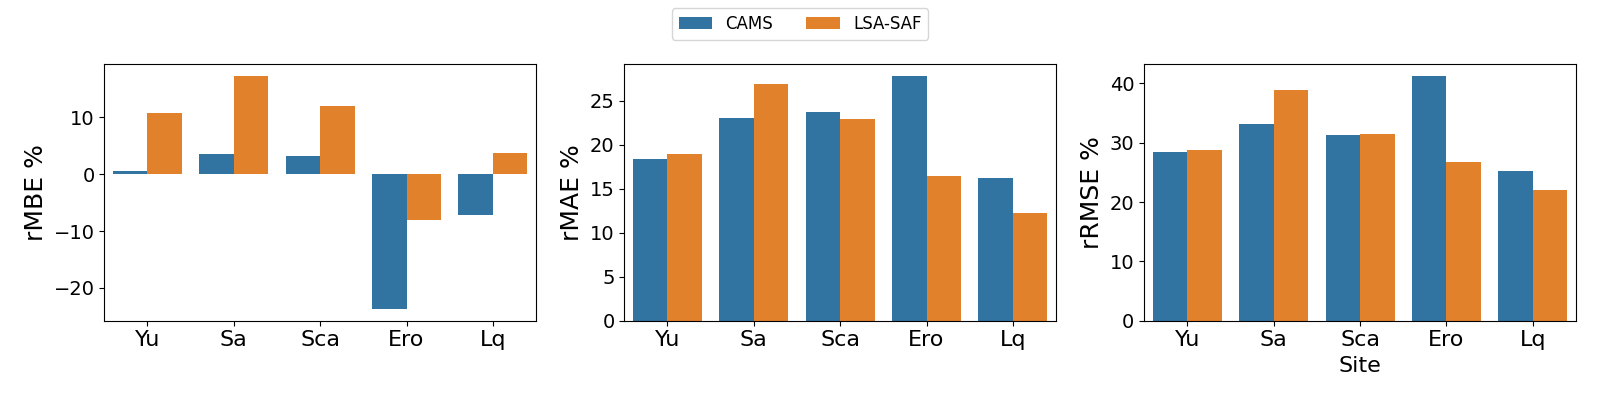
\includegraphics[width=\linewidth]{figuras/errors_15.png}
%DIFDELCMD <     %%%
%DIFDELCMD < \caption[Comparación del desempeño de los modelos CAMS y LSA-SAF en los cinco sitios de estudio.]{%
{%DIFAUXCMD
\DIFdelFL{Comparación del desempeño de los modelos CAMS y LSA-SAF en los cinco sitios de estudio (Yu, Sa, Sca, Ero y Lq) mediante las tres métricas estadísticas: MBE, MAE y RMSE expresadas en términos porcentuales relativos a escala 15-minutal.}}
    %DIFAUXCMD
%DIFDELCMD < \label{fig:general-15}
%DIFDELCMD < \end{figure}
%DIFDELCMD < 

%DIFDELCMD < \begin{figure} 
%DIFDELCMD < \centering 
%DIFDELCMD < 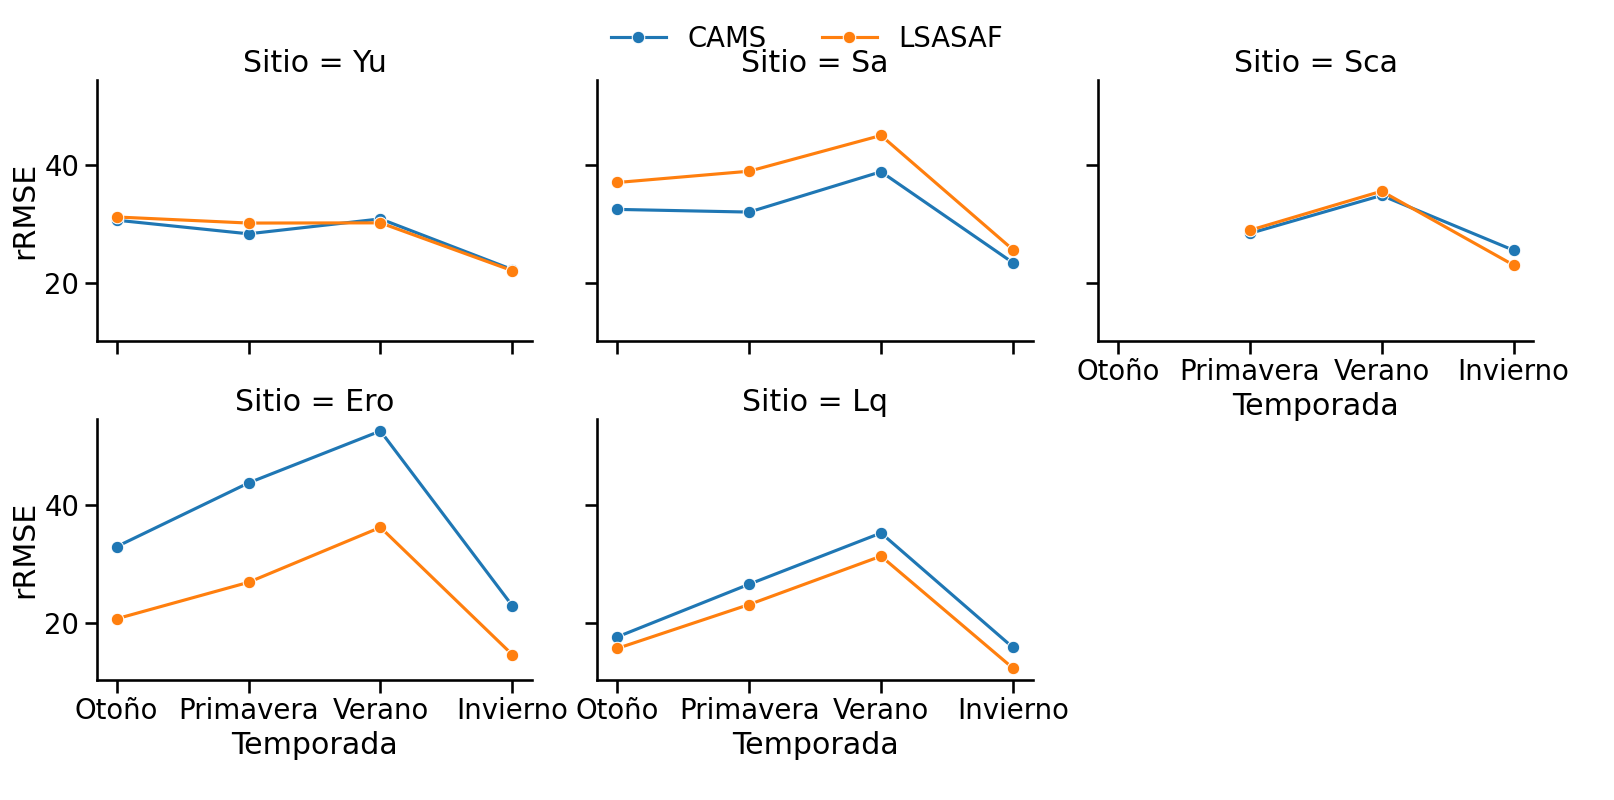
\includegraphics[width=\linewidth]{figuras/season_15_tesis.png}
%DIFDELCMD <  %%%
%DIFDELCMD < \caption[Variación estacional del rRMSE para los productos CAMS y LSA-SAF con resolución de 15 minutos.]{%
{%DIFAUXCMD
\DIFdelFL{Variación estacional del rRMSE (\%) para los productos CAMS y LSA-SAF con resolución de 15 minutos en todos los sitios de estudio. Se evidencia un aumento del error durante el verano en la mayoría de los sitios, mientras que en Yuto el rRMSE se mantiene estable, sugiriendo que la presencia de nubosidad estacional afecta de manera diferenciada la precisión de las estimaciones de radiación solar.}} 
%DIFAUXCMD
%DIFDELCMD < \label{fig:season-15} 
%DIFDELCMD < \end{figure}
%DIFDELCMD < 

%DIFDELCMD < %%%
\DIFdel{La Figura \ref{fig:season-15} muestra la variación estacional del rRMSE (\%) para los productos CAMS y LSA-SAF con resolución de 15 minutos en todos los sitios de estudio. Se observa una clara tendencia estacional en el comportamiento del error: en general, el rRMSE tiende a aumentar durante el verano, lo que indica que la precisión de las estimaciones disminuye en este período en la mayoría de los sitios. La excepción es Yuto, donde el error permanece relativamente estable a lo largo de las estaciones. Este patrón sugiere que durante el verano hay una mayor presencia de nubosidad, lo cual podría estar afectando la capacidad de los modelos satelitales para estimar correctamente la radiación solar, mientras que en otras estaciones la cobertura nubosa es menor, permitiendo estimaciones más precisas.
}%DIFDELCMD < 

%DIFDELCMD < %%%
\DIFdel{En relación con el \textit{MAE}, ambos modelos presentan magnitudes relativamente similares, aunque \textit{LSA-SAF} tiende a mostrar errores absolutos ligeramente mayores en sitios como Yu y Sa, mientras que \textit{CAMS} presenta valores más altos en Sca y Er. Esto sugiere que ninguno de los dos modelos logra una reducción clara y consistente del error en todos los sitios.
}%DIFDELCMD < 

%DIFDELCMD < %%%
\DIFdel{Por su parte, en la métrica \textit{RMSE}, que penaliza en mayor medida los errores grandes, se mantiene un patrón semejante: \textit{LSA-SAF} suele exhibir errores algo superiores a los de \textit{CAMS} en Yu y Sa, mientras que en Er y Lq la diferencia favorece al modelo satelital. En general, los resultados muestran que el desempeño relativo de los modelos depende fuertemente del sitio, sin que exista un claro ganador en todos los casos.
}%DIFDELCMD < 

%DIFDELCMD < %%%
\DIFdel{Para complementar este análisis, la Figura~\ref{fig:RMSE-variabilidad} presenta la distribución del error relativo cuadrático medio (\textit{rRMSE}) en función de dos variables explicativas: el índice de claridad ($k_t$) y un índice de variabilidad calculado a partir de la desviación estándar de las diferencias consecutivas de GHI. Este análisis bidimensional permite examinar cómo las condiciones atmosféricas locales y la estabilidad de la irradiancia influyen en la magnitud del error de los modelos.
}%DIFDELCMD < 

%DIFDELCMD < \begin{figure}[ht]
%DIFDELCMD <     \centering
%DIFDELCMD <     \includegraphics[width=\linewidth]{figuras/variabilidad.png}
%DIFDELCMD <     %%%
%DIFDELCMD < \caption[Distribución del rRMSE en función ($k_t$) y un índice de variabilidad.]{%
{%DIFAUXCMD
\DIFdelFL{Distribución del error relativo cuadrático medio (rRMSE) en función del índice de claridad ($k_t$) y un índice de variabilidad calculado a partir de la desviación estándar de las diferencias consecutivas de GHI.}}
    %DIFAUXCMD
%DIFDELCMD < \label{fig:RMSE-variabilidad}
%DIFDELCMD < \end{figure}
%DIFDELCMD < 

%DIFDELCMD < %%%
\DIFdel{El gráfico evidencia una relación clara entre el error y las condiciones radiativas:
}%DIFDELCMD < 

%DIFDELCMD < \begin{itemize}
\begin{itemize}%DIFAUXCMD
%DIFDELCMD <     \item %%%
\item%DIFAUXCMD
\DIFdel{\textbf{Patrón general con el índice de claridad ($k_t$):} En todos los sitios y para ambos modelos, el \textit{rRMSE} aumenta a medida que $k_t$ disminuye. Esto indica que los modelos tienden a desempeñarse mejor bajo condiciones despejadas ($k_t$ alto), mientras que las mayores discrepancias ocurren cuando el cielo está parcialmente nublado o cubierto ($k_t$ bajo), donde la radiación difusa domina y los modelos satelitales suelen presentar mayor incertidumbre. Este comportamiento es esperable y refuerza la sensibilidad de las estimaciones de GHI frente a la cobertura nubosa.
}%DIFDELCMD < 

%DIFDELCMD <     \item %%%
\item%DIFAUXCMD
\DIFdel{\textbf{Influencia de la variabilidad local ($\sigma$ de $\Delta GHI$):} En la mayoría de los casos, se observa un incremento del \textit{rRMSE} con la variabilidad. Cuando la variabilidad es baja ($\leq 50$ W/m$^2$), el error se mantiene reducido; sin embargo, a medida que aumenta ($\geq 150$–$200$ W/m$^2$), se aprecian regiones más intensas en el mapa (colores naranja que tienen al negro), lo que sugiere un deterioro progresivo en la estimación. Esto refleja la dificultad de los modelos para capturar fluctuaciones rápidas en la irradiancia asociadas a nubosidad variable o transiciones atmosféricas dinámicas.
}%DIFDELCMD < 

%DIFDELCMD <     \item %%%
\item%DIFAUXCMD
\DIFdel{\textbf{Comparación CAMS vs. LSA-SAF:} Ambos modelos muestran patrones similares, aunque \textit{LSA-SAF} presenta un rango de errores ligeramente más amplio, especialmente a valores bajos de $k_t$. \textit{CAMS} exhibe una distribución más homogénea, con menor saturación en los valores altos de \textit{rRMSE}. Estas diferencias podrían estar relacionadas con la resolución temporal o con las estrategias de parametrización de nubosidad empleadas por cada sistema.
}%DIFDELCMD < 

%DIFDELCMD <     \item %%%
\item%DIFAUXCMD
\DIFdel{\textbf{Variaciones entre sitios:} Aunque el patrón global es consistente, se observan diferencias notables entre sitios. Yu y Sa muestran los mayores valores de \textit{rRMSE} en condiciones de bajo $k_t$, posiblemente debido a una mayor presencia de nubosidad variable o efectos locales (por ejemplo, humedad o aerosoles). Ero y Lq presentan errores más bajos en general, lo que podría vincularse con condiciones atmosféricas más estables o una mejor respuesta del modelo en esas latitudes o altitudes. Sca muestra una dispersión más amplia, indicando una combinación de regímenes atmosféricos con distinta estabilidad.
}%DIFDELCMD < 

%DIFDELCMD <     \item %%%
\item%DIFAUXCMD
\DIFdel{\textbf{Distribución vertical del error:} La mayor concentración de error en la franja $k_t < 0.3$ en todos los casos sugiere que los modelos no representan adecuadamente los componentes difusos de la radiación. Este resultado es relevante para la calibración de modelos locales y la corrección de productos satelitales en condiciones nubladas.
}
\end{itemize}%DIFAUXCMD
%DIFDELCMD < \end{itemize}
%DIFDELCMD < 

%DIFDELCMD < %%%
\DIFdel{El índice de variabilidad empleado se define como:
}%DIFDELCMD < 

%DIFDELCMD < %%%
\begin{displaymath}
\DIFdel{\mathrm{VarIndex}(t) = 
\sigma(\Delta GHI_t) = 
\sqrt{\frac{1}{N - 1} 
\sum_{i = t - k}^{t + k} 
\left[ (GHI_i - GHI_{i-1}) - 
\overline{(GHI - GHI_{-1})} \right]^2}
}\end{displaymath}%DIFAUXCMD
%DIFDELCMD < 

%DIFDELCMD < %%%
\DIFdel{donde $GHI_i$ representa la irradiancia global horizontal en el instante $i$, 
$\Delta GHI_t = GHI_t - GHI_{t-1}$ corresponde a la diferencia temporal de GHI, 
$N$ es el número de muestras dentro de la ventana de cálculo (por ejemplo, $N = 10$), 
y $\overline{(GHI - GHI_{-1})}$ denota la media de las diferencias dentro de dicha ventana.
}%DIFDELCMD < 

%DIFDELCMD < \begin{figure}[ht]
%DIFDELCMD <     \centering
%DIFDELCMD <     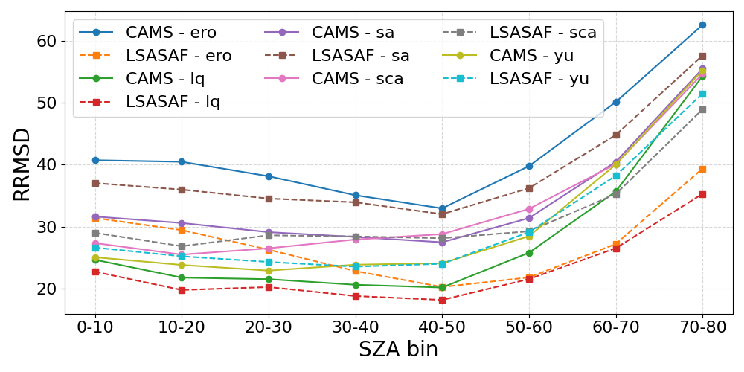
\includegraphics[width=0.8\textwidth]{figuras/RMSE-sza-15.pdf}
%DIFDELCMD <     %%%
%DIFDELCMD < \caption[Variación del error cuadrático medio relativo en función del ángulo cenital solar.]{%
{%DIFAUXCMD
\DIFdelFL{Variación del error cuadrático medio relativo (rRMSE) en función del ángulo cenital solar (SZA) para los cinco sitios analizados (Yu, Sa, Sca, Ero y Lq). Resultados para CAMS (líneas continuas) y LSA-SAF (líneas punteadas).}}
    %DIFAUXCMD
%DIFDELCMD < \label{fig:RMSE-SZA-15}
%DIFDELCMD < \end{figure}
%DIFDELCMD < 

%DIFDELCMD < %%%
\DIFdel{Por otro lado, la relación \textit{rRMSE}–SZA (Figura~\ref{fig:RMSE-SZA-15}) evidencia un comportamiento en forma de “U” invertida: los menores errores se concentran en ángulos intermedios (30°–50°), mientras que hacia ángulos bajos ($<20°$) y altos ($>70°$) el error aumenta de manera significativa. Esta tendencia se observa en los cinco sitios, con un incremento más pronunciado en Ero y Sa en las condiciones de SZA más extremas. En general, \textit{CAMS} muestra un mejor desempeño que \textit{LSA-SAF} en la mayoría de los intervalos, aunque las diferencias se reducen en los ángulos medios.
}%DIFDELCMD < 

%DIFDELCMD < %%%
\DIFdel{En conjunto, estos resultados indican que la precisión de ambos productos depende fuertemente de las condiciones atmosféricas ($k_t$) y de la geometría solar (SZA). En cielos despejados y ángulos intermedios, los errores se reducen notablemente, mientras que en condiciones nubosas y en situaciones de baja o alta elevación solar los modelos presentan las mayores limitaciones.
}%DIFDELCMD < 

%DIFDELCMD < %%%
\subsection{\DIFdel{Análisis de las estimaciones horarias}}
%DIFAUXCMD
\addtocounter{subsection}{-1}%DIFAUXCMD
%DIFDELCMD < 

%DIFDELCMD < %%%
\DIFdel{La Figura \ref{fig:general-60} presenta la evaluación comparativa del desempeño de los modelos satelitales CAMS y LSA-SAF, junto con los reanálisis ERA5 y MERRA-2, a escala horaria. En términos generales, se observa que tanto los modelos satelitales como los de reanálisis muestran un comportamiento con aparente dependencia de las condiciones de nubosidad del sitio. En localidades con predominio de cielo despejado, ambos tipos de modelos tienden a mostrar un desempeño similar, con la excepción del modelo CAMS en Ero, cuyo comportamiento particular se discute de manera separada. Por el contrario, en sitios con condiciones de nubosidad más variables, los modelos de reanálisis tienden a presentar un desempeño inferior en comparación con los modelos satelitales. Estas métricas son coincidentes con los reportes ya documentados sobre el desempeño de estos modelos en la región \citep{Ledesma2025}.}%DIFDELCMD < \\
%DIFDELCMD < 

%DIFDELCMD < \begin{figure}
%DIFDELCMD <     \centering
%DIFDELCMD <     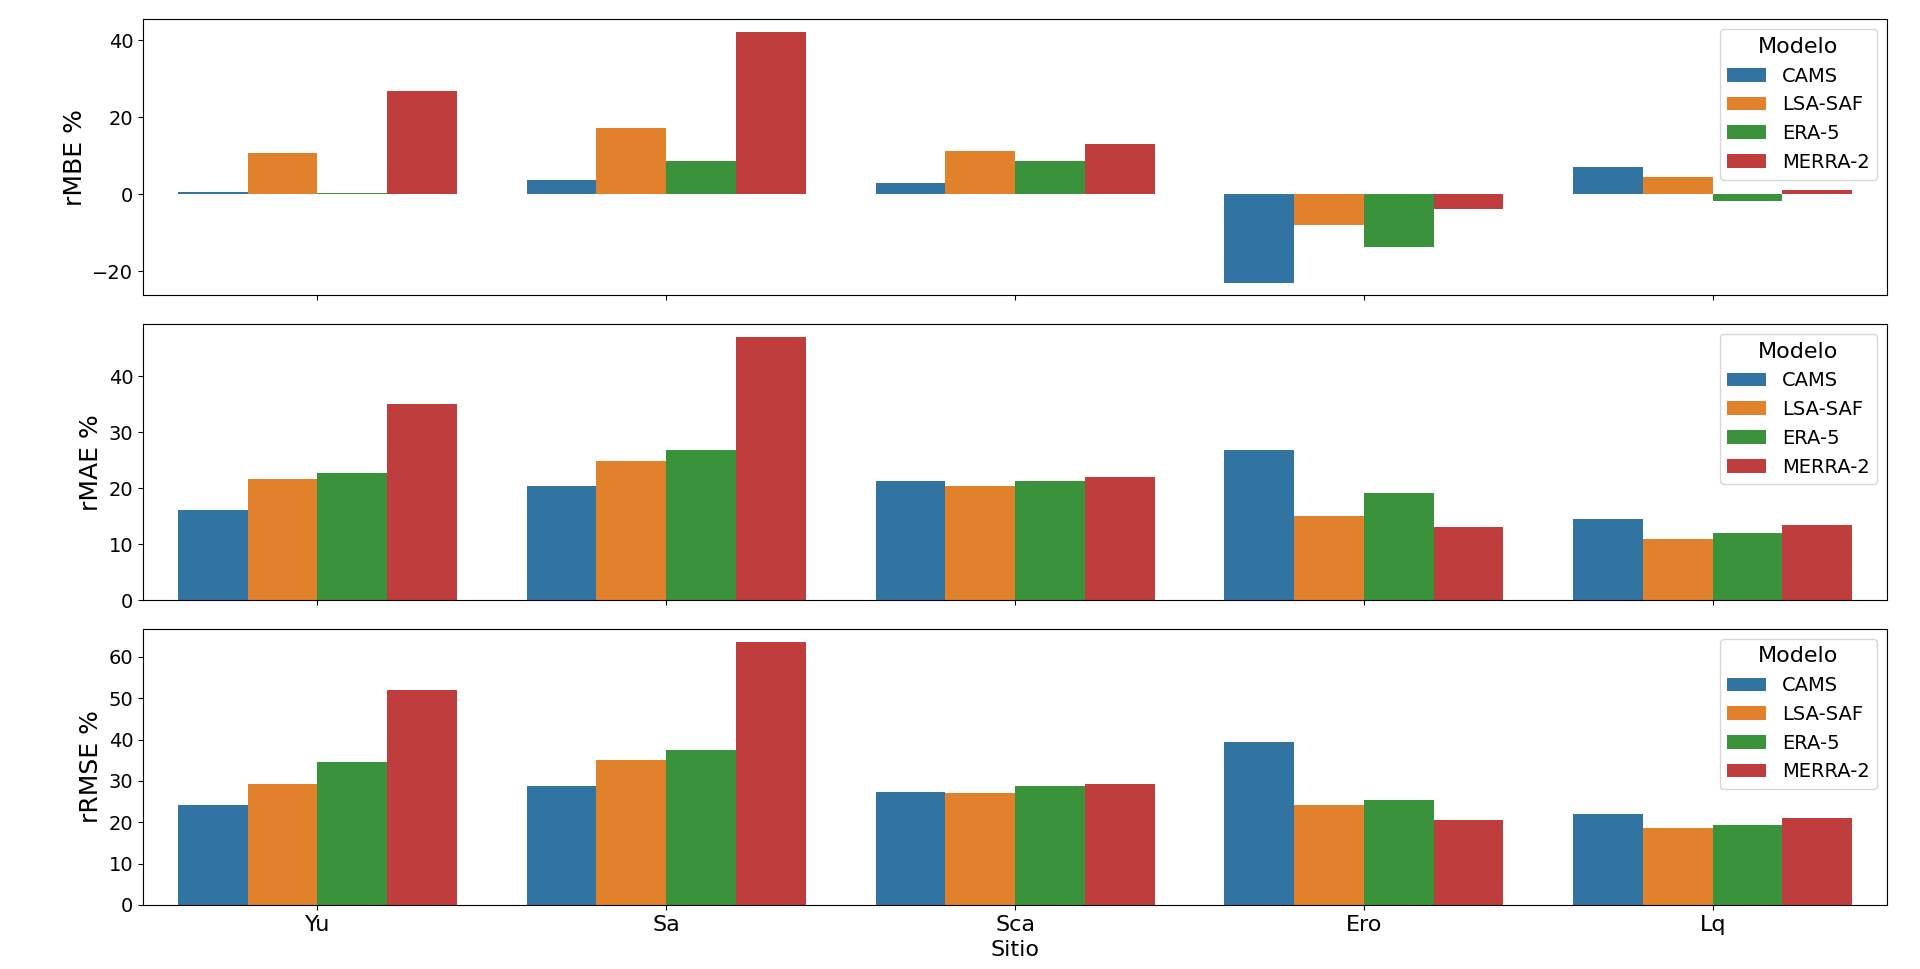
\includegraphics[width=\linewidth]{figuras/errors_60.png}
%DIFDELCMD <     %%%
%DIFDELCMD < \caption[Comparación del desempeño de los modelos satelitales y de re-análisis.]{%
{%DIFAUXCMD
\DIFdelFL{Comparación del desempeño de los modelos satelitales CAMS y LSA-SAF y de re-análisis en los cinco sitios de estudio (Yu, Sa, Sca, Er y Lq) mediante las tres métricas estadísticas: MBE, MAE y RMSE expresadas en términos porcentuales relativos a escala horaria.}}
    %DIFAUXCMD
%DIFDELCMD < \label{fig:general-60}
%DIFDELCMD < \end{figure}
%DIFDELCMD < 

%DIFDELCMD < %%%
\DIFdel{En Ero, el modelo de CAMS presenta un comportamiento atípico en su estimación. Como se observa en la Figura \ref{fig:ero}, el modelo tiende a sobreestimar la nubosidad. Este problema ya ha sido documentado por los propios desarrolladores y se ha reportado un comportamiento similar en un sitio desértico \cite{qu2017}. Según los autores, el modelo tiene dificultades para clasificar correctamente ciertos instantes despejados, que son identificados erróneamente como nubosos. Esto ocurre porque un píxel desértico puede aparecer frío en el canal térmico y brillante en el visible, lo que provoca falsos positivos de nubes en el algoritmo APOLLO/SEV.
}%DIFDELCMD < 

%DIFDELCMD < \begin{figure}
%DIFDELCMD <     \centering
%DIFDELCMD <     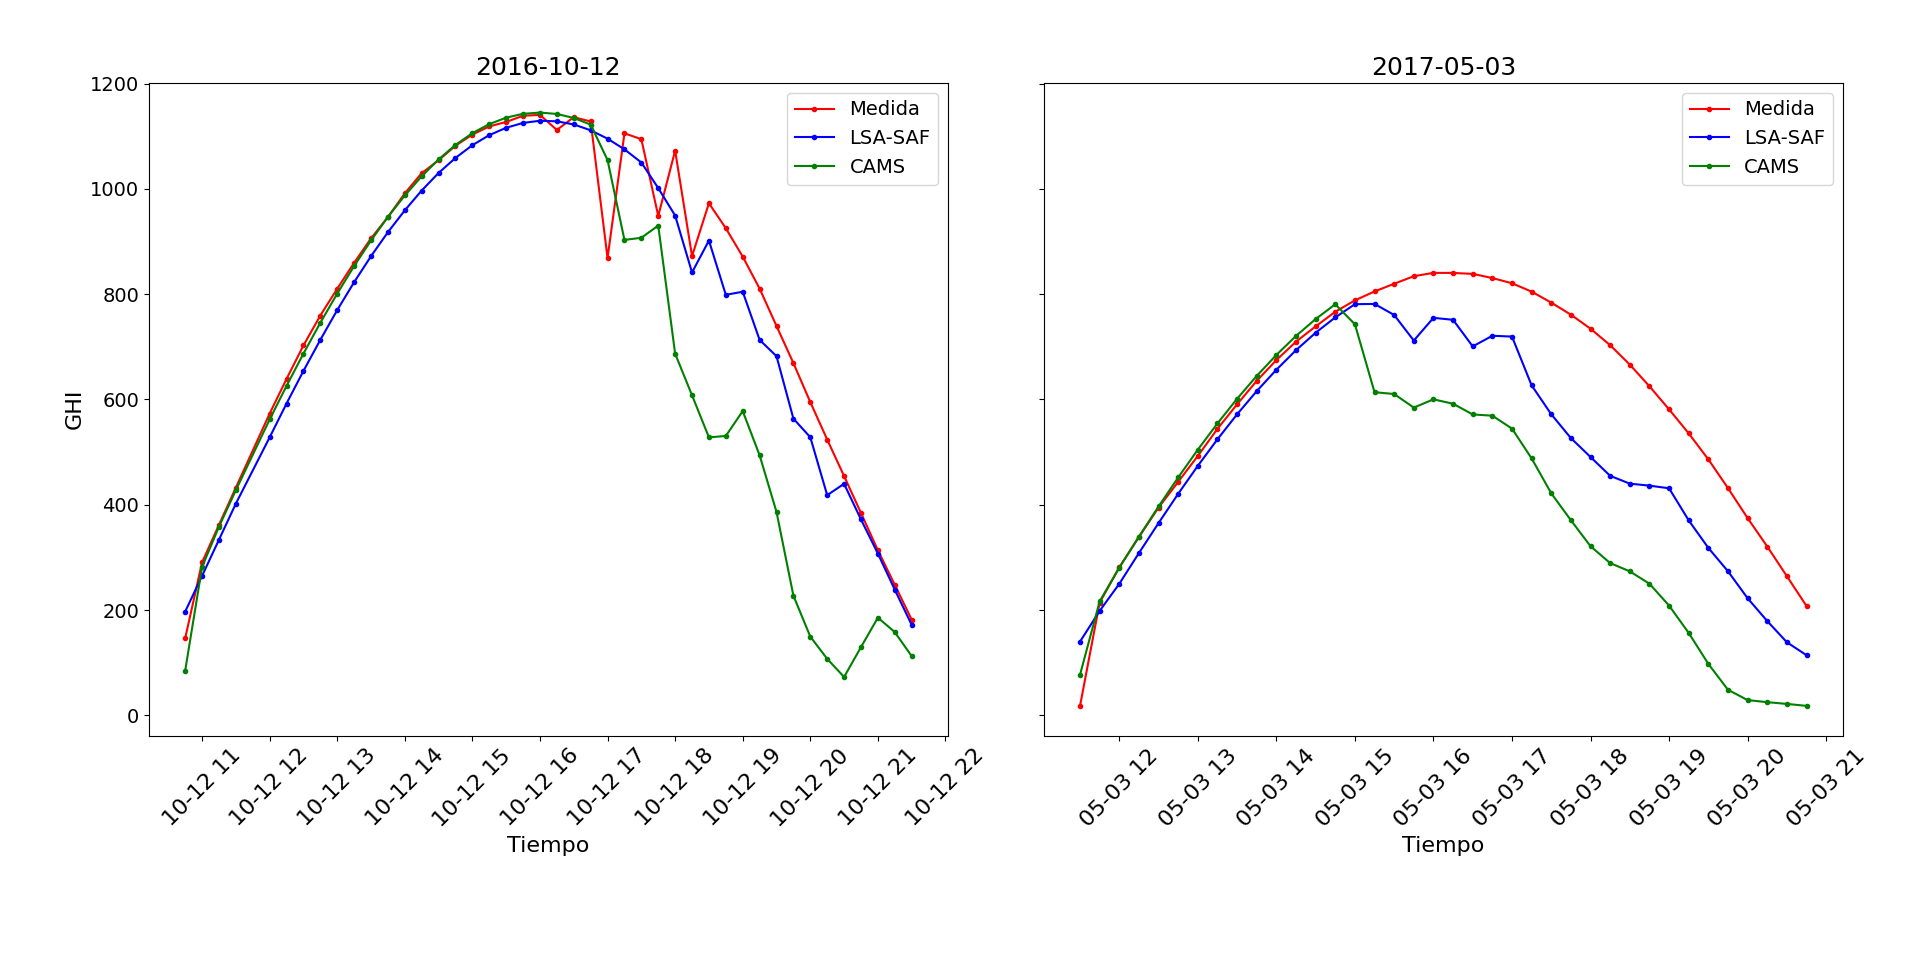
\includegraphics[width=\linewidth]{figuras/ero.png}
%DIFDELCMD <     %%%
%DIFDELCMD < \caption{%
{%DIFAUXCMD
\DIFdelFL{Comparación de la serie de GHI medida frente a las estimaciones de los modelos LSA-SAF y CAMS para dos días en Ero.}}
    %DIFAUXCMD
%DIFDELCMD < \label{fig:ero}
%DIFDELCMD < \end{figure}
%DIFDELCMD < 

%DIFDELCMD < %%%
\DIFdel{Como se ha evidenciado, el desempeño de cada modelo varía significativamente dependiendo del sitio observado, y parte de estas diferencias puede explicarse por la resolución espacial de cada modelo de estimación. La Figura \ref{fig:resoluciones} muestra un mapa de los sitios seleccionados, donde se ilustran las celdas correspondientes a los modelos MERRA2, ERA5 y LSASAF, con resoluciones de 0.5°×0.625°, 0.25°×0.25° y ~0.05°×0.05°, respectivamente.}%DIFDELCMD < \\
%DIFDELCMD < 

%DIFDELCMD < %%%
\DIFdel{Se observa que los modelos de mayor resolución, como LSASAF, representan áreas más pequeñas y detalladas alrededor de cada sitio, mientras que los modelos de resolución más gruesa, como MERRA2, generan celdas más extensas que promedian las condiciones espaciales en una región más amplia. Esta diferencia espacial es un factor determinante que puede explicar por qué los modelos de alta resolución capturan mejor la variabilidad local de las condiciones atmosféricas, mientras que los de baja resolución tienden a suavizar estas variaciones.}%DIFDELCMD < \\
%DIFDELCMD < 

%DIFDELCMD < \begin{figure}
%DIFDELCMD <     \centering
%DIFDELCMD <     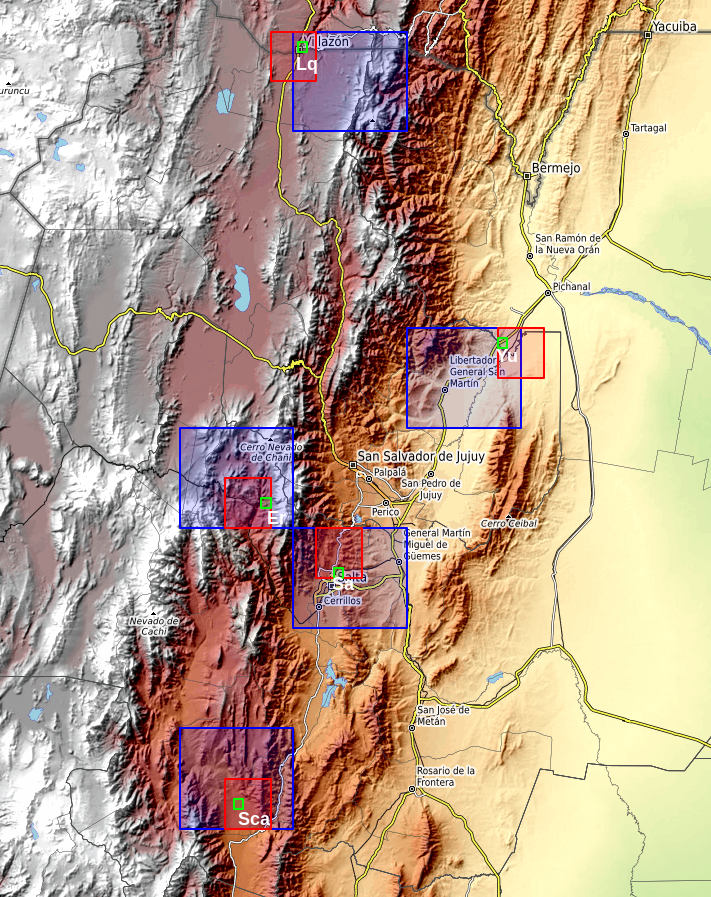
\includegraphics[width=\linewidth]{figuras/resoluciones.png}
%DIFDELCMD <     %%%
%DIFDELCMD < \caption[Mapa con perfil altitudinal para la región del NOA junto con  las celdas asociadas a los modelos.]{%
{%DIFAUXCMD
\DIFdelFL{Recorte de un mapa con perfil altitudinal para la región del NOA junto con  las celdas asociadas a los modelos MERRA-2 (azul), ERA5(rojo) y LSA-SAF(verde) en cada uno de los sitios de estudio.}}
    %DIFAUXCMD
%DIFDELCMD < \label{fig:resoluciones}
%DIFDELCMD < \end{figure}
%DIFDELCMD < 

%DIFDELCMD < %%%
\DIFdel{Esto evidencia cómo la resolución espacial influye directamente en la representación de las condiciones observadas en cada sitio, lo que subraya la importancia de seleccionar el modelo adecuado según la escala de análisis requerida.
}%DIFDELCMD < 

%DIFDELCMD < %%%
\DIFdel{Es necesario destacar que el modelo de CAMS no fue incluido explicitamente en esta comparativa puesto que, al menos en su versión web, el modelo presenta una interpolación a cada sitio de interés, sin embargo recordamos que este modelo en escencia utiliza la misma información de base que LSA-SAF.
}%DIFDELCMD < 

%DIFDELCMD < %%%
\subsection{\DIFdel{División del conjunto de datos}}
%DIFAUXCMD
\addtocounter{subsection}{-1}%DIFAUXCMD
\DIFdel{De acuerdo a lo indicado en la sección \ref{MLM} el conjunto de datos debe ser segmentado con fin de evaluar el rendimiento de los modelos de aprendizaje automático utilizados en la regresión del proceso de adaptación al sitio y controlar el sobre-entrenamiento de los modelos. En el contexto de AS en los trabajos \cite{POLO2016, POLO2020} se recomienda tomar al menos un año de medidas para la calibración de los modelos. Siguiendo estas ideas el conjunto de medidas fue dividido en subconjunto de entrenamiento, validación y prueba.  
}%DIFDELCMD < 

%DIFDELCMD < \begin{table}[ht]
%DIFDELCMD <     \centering
%DIFDELCMD <     \renewcommand{\arraystretch}{1.5} %%%
%DIF <  Espaciado vertical en la tabla
    %DIFDELCMD < \begin{tabular}{|>{\centering\arraybackslash}p{2cm}|>{\centering\arraybackslash}p{3cm}|>{\centering\arraybackslash}p{3cm}|>{\centering\arraybackslash}p{4cm}|}
%DIFDELCMD <         \hline
%DIFDELCMD <         %%%
\DIFdelFL{\textbf{ID} }%DIFDELCMD < & %%%
\DIFdelFL{\textbf{Entrenamiento} }%DIFDELCMD < & %%%
\DIFdelFL{\textbf{Validación} }%DIFDELCMD < & %%%
\DIFdelFL{\textbf{Prueba}}%DIFDELCMD < \\ 
%DIFDELCMD <         \hline
%DIFDELCMD < 

%DIFDELCMD <         %%%
\DIFdelFL{\textbf{YU}  }%DIFDELCMD < & %%%
\DIFdelFL{2017 }%DIFDELCMD < & %%%
\DIFdelFL{2017 }%DIFDELCMD < & %%%
\DIFdelFL{2018 }%DIFDELCMD < \\ 
%DIFDELCMD <         %%%
\DIFdelFL{\textbf{SA}  }%DIFDELCMD < & %%%
\DIFdelFL{2009 }%DIFDELCMD < & %%%
\DIFdelFL{2009 }%DIFDELCMD < & %%%
\DIFdelFL{2010 - 2024 }%DIFDELCMD < \\ 
%DIFDELCMD <         %%%
\DIFdelFL{\textbf{SCA} }%DIFDELCMD < & %%%
\DIFdelFL{2013 }%DIFDELCMD < & %%%
\DIFdelFL{2013 }%DIFDELCMD < & %%%
\DIFdelFL{2012-2014 }%DIFDELCMD < \\
%DIFDELCMD <         %%%
\DIFdelFL{\textbf{ERO} }%DIFDELCMD < & %%%
\DIFdelFL{2013 }%DIFDELCMD < & %%%
\DIFdelFL{2013 }%DIFDELCMD < & %%%
\DIFdelFL{2014 - 2024  }%DIFDELCMD < \\
%DIFDELCMD <         %%%
\DIFdelFL{\textbf{LQ}  }%DIFDELCMD < & %%%
\DIFdelFL{2019 }%DIFDELCMD < & %%%
\DIFdelFL{2019 }%DIFDELCMD < & %%%
\DIFdelFL{2018, 2021 - 2023  }%DIFDELCMD < \\
%DIFDELCMD <     \hline
%DIFDELCMD <     \end{tabular}
%DIFDELCMD <     %%%
%DIFDELCMD < \caption{%
{%DIFAUXCMD
\DIFdelFL{División del conjunto de datos en entrenamiento, validación y prueba.}}
    %DIFAUXCMD
%DIFDELCMD < \label{tab:tvt}
%DIFDELCMD < \end{table}
%DIFDELCMD < 

%DIFDELCMD <     
%DIFDELCMD < \begin{table*}%%%
%DIF < []
  %DIFDELCMD < \centering
%DIFDELCMD <   %%%
%DIFDELCMD < \caption[Métricas de desempeño para cada modelo en el conjunto de pruebas.]{%
{%DIFAUXCMD
\DIFdelFL{Métricas de desempeño (MBE, MAE, RMSE) para cada modelo y conjunto de datos satelitales en los cinco sitios en el \textbf{conjunto de pruebas}. 
   }%DIFDELCMD < \label{tbl:metrics_test}
%DIFDELCMD <            %%%
\DIFdelFL{Los valores están normalizados y expresados como porcentajes relativos al promedio de GHI en cada sitio: 
           396.8~W/m$^{2}$ (Yu), 397~W/m$^{2}$ (Sa), 557.1~W/m$^{2}$ (Sca), 690.6~W/m$^{2}$ (Ero) y 673.7~W/m$^{2}$ (Lq).}}
  %DIFAUXCMD
%DIFDELCMD < \resizebox{\linewidth}{!}{%
%DIFDELCMD <     \begin{tabular}{|l|ccc|ccc|ccc|ccc|ccc|}
%DIFDELCMD <       \hline
%DIFDELCMD <       & \multicolumn{3}{c|}{YU} & \multicolumn{3}{c|}{SA} & \multicolumn{3}{c|}{SCA} & \multicolumn{3}{c|}{ERO} & \multicolumn{3}{c|}{LQ} \\
%DIFDELCMD <       \cline{2-16}
%DIFDELCMD <       Modelo  & MBE & MAE & RMSE & MBE & MAE & RMSE & MBE & MAE & RMSE & MBE & MAE & RMSE & MBE & MAE & RMSE \\
%DIFDELCMD <       \hline
%DIFDELCMD <       \multicolumn{16}{|c|}{\textit{Resolución Temporal: 15 minutos}} \\
%DIFDELCMD <       \hline
%DIFDELCMD <       CAMS      & -0.2 & 17.4 & 27.2 & 3.9  & 23.4 & 33.7 & 2.6  & 21.8 & 29.8 & -23.6 & 27.6 & 40.9 & -6.9 & 16.5 & 25.8 \\
%DIFDELCMD <       LSA-SAF & 7.6  & 16.5 & 25.5 & 17.9 & 27.4 & 39.4 & 13.1 & 22.2 & 30.9 & -7.7  & 16.2 & 26.5 & 4.0  & 12.6 & 22.6 \\
%DIFDELCMD <       \hline
%DIFDELCMD <       \multicolumn{16}{|c|}{\textit{Resolución Temporal: horaria}} \\
%DIFDELCMD <       \hline
%DIFDELCMD <       CAMS    & -0.1 & 15.2 & 23.5 & 4.0 & 20.9 & 29.3 & 3.0 & 19.7 & 26.1 & -23.6 & 26.6 & 39.3 & -4.8 & 14.5 & 21.6 \\
%DIFDELCMD <       LSA-SAF & 7.5  & 14.4 & 21.8 & 17.9 & 25.3 & 35.7 & 13.3 & 20.3 & 27.1 & -7.7  & 14.8 & 24.0 & 4.8  & 10.9 & 18.2 \\
%DIFDELCMD <       ERA5    & 1.2  & 22.2 & 33.7 & 9.4  & 27.1 & 37.7 & 1.9  & 20.2 & 29.7 & -14.0 & 19.3 & 25.6 & -0.8 & 11.3 & 18.4 \\
%DIFDELCMD <       MERRA-2 & 24.9 & 33.5 & 51.2 & 43.4 & 48.3 & 65.0 & 10.9 & 21.7 & 30.3 & -3.8  & 13.1 & 20.4 & 1.4  & 13.4 & 20.8 \\
%DIFDELCMD <       \hline
%DIFDELCMD <     \end{tabular}%
%DIFDELCMD <   }
%DIFDELCMD < \end{table*}
%DIFDELCMD < 

%DIFDELCMD <     
%DIFDELCMD < %%%
\section{\DIFdel{Adaptación al sitio con una variable descriptiva}}%DIFAUXCMD
\addtocounter{section}{-1}%DIFAUXCMD
%DIFDELCMD < \label{sec:01}
%DIFDELCMD < 

%DIFDELCMD < %%%
\DIFdel{En los trabajos citados en la Sección \ref{ch_3} sobre la evaluación del proceso de Adaptación al Sitio (SA), se ha prestado escasa atención a las razones subyacentes por las cuales ciertos modelos de aprendizaje automático (ML) superan a otros en este proceso. Dado que algunos modelos de ML poseen una naturaleza inherentemente más compleja que otros, podría suponerse que los modelos más complejos ofrecerían un rendimiento superior frente a aquellos de menor complejidad. En este contexto, el término complejidad hace referencia tanto a la complejidad computacional —es decir, la cantidad de operaciones necesarias para ejecutar el modelo— como a la complejidad conceptual, relacionada con el nivel de conocimiento requerido para comprender su funcionamiento.}%DIFDELCMD < \\
%DIFDELCMD < 

%DIFDELCMD < %%%
\DIFdel{En esta sección se presenta una implementación del proceso de SA basada en uno de los enfoques clásicos, que consiste en adaptar una serie temporal modelada (proveniente de datos satelitales o de reanálisis) utilizando como referencia una serie de mediciones in situ.}%DIFDELCMD < \\
%DIFDELCMD < 

%DIFDELCMD < %%%
\DIFdel{Dado que el modelo de Regresión Lineal Simple (SLR por sus siglas en ingles) puede considerarse el menos complejo entre los empleados en este estudio, la primera evaluación del proceso de SA es realizada utilizando este modelo de regresión. El objetivo es comparar el desempeño de SLR con el de modelos de regresión más complejos, como el Perceptrón Multicapa (MLP) y XGBoost (XGB), utilizando las mismas métricas de evaluación.}%DIFDELCMD < \\
%DIFDELCMD < 

%DIFDELCMD < %%%
\DIFdel{Para los modelos MLP y XGB, la determinación de la configuración óptima de hiperparámetros fue fundamental para lograr un desempeño consistente en las particiones de validación cruzada. Esto se llevó a cabo mediante una búsqueda exhaustiva en rejilla (Grid Search) implementada con la función \textbf{GridSearchCV} de la biblioteca \textbf{Scikit-learn} en Python \citep{Pedregosa2012}. Los rangos específicos de hiperparámetros evaluados para MLP y XGBoost se presentan en la Tabla \ref{tab:gridsearch}. La selección de hiperparámetros óptimos constituye un paso crítico en el aprendizaje automático, ya que influye directamente en la complejidad del modelo, su capacidad de generalización y su rendimiento predictivo global \citep{Goodfellow2016}.}%DIFDELCMD < \\
%DIFDELCMD < 

%DIFDELCMD < \begin{table}[ht]
%DIFDELCMD < %%%
%DIFDELCMD < \caption{%
{%DIFAUXCMD
\DIFdelFL{Espacio cartesiano de hiperparámetros para las técnicas de aprendizaje supervisado.}}
%DIFAUXCMD
%DIFDELCMD < \label{tab:gridsearch}
%DIFDELCMD < \centering
%DIFDELCMD < \resizebox{\linewidth}{!} {
%DIFDELCMD < \def\arraystretch{1.5}
%DIFDELCMD < \begin{tabular}{lcccc}
%DIFDELCMD < \hline
%DIFDELCMD < %%%
\DIFdelFL{\textbf{Hiperparámetro} }%DIFDELCMD < & %%%
\DIFdelFL{\textbf{Inferior} }%DIFDELCMD < & %%%
\DIFdelFL{\textbf{Superior} }%DIFDELCMD < & %%%
\DIFdelFL{\textbf{Paso} }%DIFDELCMD < & %%%
\DIFdelFL{\textbf{Función de transformación} }%DIFDELCMD < \\
%DIFDELCMD < \hline
%DIFDELCMD < %%%
\DIFdelFL{MLP}%DIFDELCMD < \\
%DIFDELCMD < \hline
%DIFDELCMD <  %%%
\DIFdelFL{Capas ocultas        }%DIFDELCMD < & %%%
\DIFdelFL{1    }%DIFDELCMD < & %%%
\DIFdelFL{3     }%DIFDELCMD < & %%%
\DIFdelFL{1   }%DIFDELCMD < & %%%
\DIFdelFL{- }%DIFDELCMD < \\
%DIFDELCMD <  %%%
\DIFdelFL{Nodos ocultos        }%DIFDELCMD < & %%%
\DIFdelFL{1    }%DIFDELCMD < & %%%
\DIFdelFL{4     }%DIFDELCMD < & %%%
\DIFdelFL{1   }%DIFDELCMD < & %%%
\DIFdelFL{$2^{x}$ }%DIFDELCMD < \\
%DIFDELCMD <  %%%
\DIFdelFL{Fracción de dropout  }%DIFDELCMD < & %%%
\DIFdelFL{0    }%DIFDELCMD < & %%%
\DIFdelFL{0.3   }%DIFDELCMD < & %%%
\DIFdelFL{0.1 }%DIFDELCMD < & %%%
\DIFdelFL{- }%DIFDELCMD < \\
%DIFDELCMD <  %%%
\DIFdelFL{Tasa de aprendizaje  }%DIFDELCMD < & %%%
\DIFdelFL{-3   }%DIFDELCMD < & %%%
\DIFdelFL{-1    }%DIFDELCMD < & %%%
\DIFdelFL{1   }%DIFDELCMD < & %%%
\DIFdelFL{$10^{x}$ }%DIFDELCMD < \\
%DIFDELCMD < \hline
%DIFDELCMD < %%%
\DIFdelFL{XGBoost}%DIFDELCMD < \\
%DIFDELCMD < \hline
%DIFDELCMD < %%%
\DIFdelFL{Booster               }%DIFDELCMD < & %%%
\DIFdelFL{gbtree }%DIFDELCMD < & & & \\
%DIFDELCMD <  %%%
\DIFdelFL{Estimadores          }%DIFDELCMD < & %%%
\DIFdelFL{1    }%DIFDELCMD < & %%%
\DIFdelFL{50    }%DIFDELCMD < & %%%
\DIFdelFL{10  }%DIFDELCMD < & %%%
\DIFdelFL{- }%DIFDELCMD < \\
%DIFDELCMD <  %%%
\DIFdelFL{Profundidad máxima   }%DIFDELCMD < & %%%
\DIFdelFL{2    }%DIFDELCMD < & %%%
\DIFdelFL{5     }%DIFDELCMD < & %%%
\DIFdelFL{1   }%DIFDELCMD < & %%%
\DIFdelFL{$2^{x}$ }%DIFDELCMD < \\
%DIFDELCMD <  %%%
\DIFdelFL{Tasa de aprendizaje  }%DIFDELCMD < & %%%
\DIFdelFL{-3   }%DIFDELCMD < & %%%
\DIFdelFL{-1    }%DIFDELCMD < & %%%
\DIFdelFL{1   }%DIFDELCMD < & %%%
\DIFdelFL{$10^{x}$ }%DIFDELCMD < \\
%DIFDELCMD < \hline
%DIFDELCMD < \end{tabular}}
%DIFDELCMD < \end{table}
%DIFDELCMD < 

%DIFDELCMD < %%%
\DIFdel{En cuanto al preprocesamiento de los datos de entrada, la normalización o el escalado de características es una práctica común en aprendizaje automático para mejorar la convergencia y la estabilidad, particularmente en modelos sensibles a la magnitud de las variables de entrada. Sin embargo, en esta evaluación \textbf{no se aplicó normalización}, ya que no se consideró necesaria para los modelos y datos utilizados.  
}%DIFDELCMD < 

%DIFDELCMD < %%%
\DIFdel{En el caso del modelo SLR, el escalado de la variable independiente no es necesario porque el modelo es inherentemente invariante al escalado: multiplicar la entrada por un factor constante provoca un cambio inversamente proporcional en el coeficiente de la pendiente, dejando las predicciones sin alterar.  
}%DIFDELCMD < 

%DIFDELCMD < %%%
\DIFdel{De manera similar, XGB, cuando se implementa con árboles de decisión como aprendices base, \textbf{no requiere escalado de características}, ya que las divisiones en los nodos dependen del \textbf{orden relativo} de los valores y no de sus magnitudes absolutas \cite{Soria2022, Chen2016}.  
}%DIFDELCMD < 

%DIFDELCMD < %%%
\DIFdel{En el caso del modelo MLP, el escalado puede ser importante cuando las variables de entrada difieren significativamente en su rango o unidades. Sin embargo, en el presente estudio se utilizó \textbf{una sola variable de entrada} (GHI derivado de satélite), expresada en las \textbf{mismas unidades y rango} que la variable objetivo (GHI medido en superficie). Por lo tanto, no se consideró necesaria ninguna normalización adicional.}%DIFDELCMD < \\
%DIFDELCMD < 

%DIFDELCMD < \begin{table*}[h]
%DIFDELCMD <   \centering
%DIFDELCMD <   

%DIFDELCMD <   %%%
%DIFDELCMD < \caption[Métricas de desempeño para cada modelo adaptado en el conjunto de pruebas.]{%
{%DIFAUXCMD
\DIFdelFL{Métricas de desempeño (MBE, MAE, RMSE) para cada modelo adaptado en los cinco sitios en el \textbf{conjunto de pruebas.}}}
  %DIFAUXCMD
%DIFDELCMD < \label{tab:metrics-as-1}
%DIFDELCMD <   \resizebox{\linewidth}{!}{%
%DIFDELCMD <     \begin{tabular}{|l|ccc|ccc|ccc|ccc|ccc|}
%DIFDELCMD <       \hline
%DIFDELCMD <       & \multicolumn{3}{c|}{YU} & \multicolumn{3}{c|}{SA} & \multicolumn{3}{c|}{SCA} & \multicolumn{3}{c|}{ERO} & \multicolumn{3}{c|}{LQ} \\
%DIFDELCMD <       \cline{2-16}
%DIFDELCMD <       Modelo  & MBE & MAE & RMSE & MBE & MAE & RMSE & MBE & MAE & RMSE & MBE & MAE & RMSE & MBE & MAE & RMSE \\
%DIFDELCMD <       \hline
%DIFDELCMD <       \multicolumn{16}{|c|}{\textit{Resolución Temporal: 15 minutos}} \\
%DIFDELCMD <       \hline
%DIFDELCMD <       CAMS SLR    & -0.9 & 17.1 & 26.4 &  3.8 & 21.3 & 31.5 & -1.5 & 18.4 & 26.0 &  2.5 & 24.8 & 31.5 &  2.1 & 15.9 & 23.5 \\
%DIFDELCMD <       CAMS MLP    & -4.4 & 17.7 & 26.2 &  4.8 & 21.4 & 31.6 &  7.7 & 17.8 & 27.7 &  0.5 & 24.1 & 31.2 &  9.1 & 19.4 & 25.6 \\
%DIFDELCMD <       CAMS XGB    & -1.3 & 17.1 & 26 &  3.8 & 21.4 & 31.4 & -1.8 & 18.9 & 26.2 &  2.5 & 23.9 & 30.9 &  2.2 & 15.9 & 23.5 \\
%DIFDELCMD <       \hline
%DIFDELCMD <       LSASAF SLR  & -5.5 & 18.4 & 25 &  4.4 & 23.9 & 34.6 &  1.0 & 18.0 & 26.7 &  2.7 & 17.1 & 25.4 &  2.2 & 12.9 & 22.3 \\
%DIFDELCMD <       LSASAF MLP  & -7.1 & 18.6 & 25 &  4.5 & 23.6 & 34.5 &  5.9 & 18.4 & 26.6 &  2.5 & 17.0 & 25.3 & -0.4 & 13.6 & 22.1 \\    
%DIFDELCMD <       LSASAF XGB  & -6.0 & 18.2 & 24 &  4.3 & 23.9 & 34.6 &  0.5 & 18.6 & 27.0 &  2.4 & 17.2 & 25.1 &  2.3 & 13.1 & 22.3 \\
%DIFDELCMD <       \hline
%DIFDELCMD <       \multicolumn{16}{|c|}{\textit{Resolución Temporal: horaria}} \\
%DIFDELCMD <       \hline
%DIFDELCMD <       CAMS SLR    &  -0.5 & 14.7 & 22.6 &  3.5 & 18.5 & 27.0 & -1.7 & 15.9 & 22.0 &  2.1 & 23.4 & 29.6 &  2.6 & 13.8 & 19.4 \\
%DIFDELCMD <       CAMS MLP    & -2.0 & 14.8 & 22.4 &  4.3 & 18.6 & 27.2 & -4.0 & 16.6 & 22.4 &  3.8 & 23.5 & 29.5 & -0.5 & 13.0 & 19.2 \\
%DIFDELCMD < 	  CAMS XGB    & -1.4& 15.9 & 23   &  3.4 & 18.9 & 27.1 & -2.4 & 16.6 & 22.4 &  2.1 & 22.8 & 29.2 &  2.7 & 13.9 & 19.6 \\      
%DIFDELCMD <       \hline
%DIFDELCMD <       LSASAF SLR  &  -5.2 & 15.8 & 21.2 &  4.3 & 21.2 & 30.5 &  1.1 & 15.6 & 22.7 &  2.5 & 15.7 & 22.8 &  0.3 & 10.6 & 17.4 \\
%DIFDELCMD <       LSASAF MLP  & -6.8 & 16.4 & 21.4 &  2.5 & 21.4 & 30.2 &  8.3 & 16.1 & 24.1 &  9.6 & 19.4 & 24.6 & -3.8 & 12.1 & 17.8 \\
%DIFDELCMD <       LSASAF XGB  & -0.9& 16.3 & 21.5 &  4.1 & 21.4 & 30.6 &  0 & 16.9 & 23.4 &  2.2 & 15.9 & 22.6 &  0.2 & 10.9 & 17.4 \\
%DIFDELCMD <       

%DIFDELCMD <       \hline
%DIFDELCMD <       ERA-5 SLR   &   2.7 & 22.6 & 33.7 &  6.4 & 26.5 & 36.9 & -6.4 & 20.1 & 29.1 & -0.6 & 15.4 & 21.4 &  2.1 & 11.6 & 18.4 \\     
%DIFDELCMD <       ERA-5 MLP   & 0.0  & 22.5 & 33.7 &  9.6 & 27.1 & 37.6 & -1.8 & 19.0 & 28.5 & -7.5 & 16.7 & 23.1 &  0.1 & 11.3 & 18.3 \\ 
%DIFDELCMD <       ERA-5 XGB   & -1.4& 23.4 & 33.5 &  6.3 & 27.3 & 37.4 & -7.3 & 20.7 & 29.3 & -0.5 & 15.2 & 21.2 &  2.0 & 11.8 & 18.6 \\
%DIFDELCMD <       \hline
%DIFDELCMD <       MERRA-2 SLR &  -2.6 & 34.5 & 44   &  7.1 & 35.2 & 46.0 & -2.2 & 20.3 & 27.7 &  0.7 & 12.9 & 20.1 &  0.3 & 13.1 & 20.4 \\
%DIFDELCMD <       MERRA-2 MLP & 1.7  & 31.5 & 47.8 &  0.8 & 36.3 & 45.4 & -0.3 & 19.5 & 27.5 & 11.7 & 17.5 & 23.4 & -2.8 & 13.4 & 20.6 \\
%DIFDELCMD <       MERRA-2 XGB & 1.5 & 33.4 & 42.4 & 6.9 & 35.6 & 46.1 & -2.8 & 20.8 & 28.2 &  0.8 & 13.3 & 20.3 &  0.2 & 13.5 & 20.6 \\
%DIFDELCMD <       \hline
%DIFDELCMD <     \end{tabular}%
%DIFDELCMD <   }
%DIFDELCMD < \end{table*}
%DIFDELCMD < 

%DIFDELCMD < %%%
\DIFdel{Los resultados resumidos en la Tabla \ref{tab:metrics-as-1} reflejan un comportamiento consistente entre los diferentes enfoques de modelado y las fuentes de datos satelitales. En términos generales, las ganancias según las métricas normalizadas que (MBE, MAE y RMSE) permanecen dentro de rangos comparables para todas las combinaciones de modelos y productos, sin evidenciar diferencias estadísticamente significativas entre los modelos lineales (SLR) y los no lineales (MLP, XGB). Este comportamiento sugiere que, bajo las condiciones actuales de los conjuntos de datos modelados, los modelos de regresión simples logran capturar gran parte de la variabilidad entre la irradiancia estimada y la medida en superficie, con un costo computacional significativamente menor.}%DIFDELCMD < \\
%DIFDELCMD < 

%DIFDELCMD < %%%
\DIFdel{Particularmente, el modelo SLR mostró un desempeño competitivo respecto a los modelos más complejos, lo cual coincide con observaciones previas en estudios de adaptación de sitio, donde las mejoras marginales obtenidas por métodos no lineales no siempre justifican su mayor complejidad. En efecto, \citep{Fernández2020} demostraron que la corrección empírica mediante regresión y mapeo cuantil puede reducir el sesgo relativo de la GHI a valores cercanos a cero, mientras que \citep{ZAINALI2024} observaron que el rendimiento de modelos basados en aprendizaje automático (como XGBoost o redes neuronales) depende fuertemente del régimen climático local, sin que exista un modelo universalmente superior.
}%DIFDELCMD < 

%DIFDELCMD < %%%
\DIFdel{Asimismo, se observó que los patrones de desempeño inicial de cada producto satelital se mantienen tras la adaptación, lo que refuerza la hipótesis de que el proceso de calibración no altera sustancialmente la estructura del error inherente al origen del dato. Esto concuerda con lo señalado por \cite{POLO2020}, quienes destacan que la efectividad de la adaptación depende tanto de la calidad del producto de entrada como de la representatividad temporal de las mediciones de superficie empleadas para la corrección.
}%DIFDELCMD < 

%DIFDELCMD < %%%
\DIFdel{Por otra parte, el incremento en la complejidad del modelo no se tradujo en mejoras significativas en las métricas globales de desempeño. Este resultado es consistente con los hallazgos de \citep{Quansah2024}, quienes al aplicar corrección de sesgo a productos de reanálisis (NASA-POWER) en regiones tropicales, encontraron que métodos relativamente simples como la correspondencia de funciones de distribución acumulada (CDF) fueron suficientes para reducir los errores sistemáticos sin comprometer la coherencia temporal y espacial del recurso solar.
}%DIFDELCMD < 

%DIFDELCMD < %%%
\DIFdel{En este sentido, la estabilidad observada del modelo SLR frente al ruido y las limitaciones del conjunto de entrenamiento sugiere que, para las condiciones locales de los sitios analizados, la relación entre las variables de entrada (GHI modelada) y la irradiancia medida puede describirse de manera robusta mediante modelos lineales. Tal comportamiento también ha sido documentado en estudios de latitudes altas, como el de \citep{ZAINALI2024}, donde se concluye que la adaptación de sitio es un proceso fuertemente dependiente de las condiciones espacio-temporales y que la ganancia en precisión ofrecida por técnicas de aprendizaje automático solo se manifiesta cuando existe suficiente heterogeneidad en los datos o presencia de no linealidades marcadas.
}%DIFDELCMD < 

%DIFDELCMD < %%%
\DIFdel{Finalmente, estos resultados respaldan la aplicabilidad de estrategias de adaptación de sitio basadas en modelos simples en contextos donde los datos satelitales presentan buena calidad intrínseca y se dispone de series cortas de medición en superficie. En tales escenarios, la implementación de modelos parsimoniosos como SLR puede ofrecer un equilibrio óptimo entre precisión, interpretabilidad y eficiencia computacional, consolidando su utilidad en la mejora operativa de productos satelitales de irradiancia solar y en la planificación de sistemas fotovoltaicos locales.
}%DIFDELCMD < 

%DIFDELCMD < \begin{figure}[ht]
%DIFDELCMD < \centering
%DIFDELCMD < \begin{tikzpicture}
%DIFDELCMD < \begin{axis}[
%DIFDELCMD <     ybar,
%DIFDELCMD <     bar width=7pt,
%DIFDELCMD <     width=\linewidth,
%DIFDELCMD <     height=8cm,
%DIFDELCMD <     ylabel={rRMSE (\%)},
%DIFDELCMD <     xlabel={Sitios},
%DIFDELCMD <     symbolic x coords={YU, SA, SCA, ERO, LQ},
%DIFDELCMD <     xtick=data,
%DIFDELCMD <     xticklabel style={rotate=45, anchor=east},
%DIFDELCMD <     enlarge x limits=0.1,
%DIFDELCMD <     ymin=0,
%DIFDELCMD <     nodes near coords,
%DIFDELCMD <     nodes near coords style={font=\scriptsize, rotate=90, anchor=west, text=black!85},
%DIFDELCMD <     legend style={at={(0.5,-0.30)}, anchor=north, legend columns=4, font=\small},
%DIFDELCMD <     cycle list={{blue!70},{blue!40},{cyan!60},{green!60},{red!70},{red!40},{orange!60},{purple!60}}
%DIFDELCMD < ]
%DIFDELCMD < 

%DIFDELCMD < % ---- CAMS sin adaptar ----
%DIFDELCMD < \addplot+[fill=blue!70] coordinates {(YU,27.2) (SA,33.7) (SCA,29.8) (ERO,40.9) (LQ,25.8)};
%DIFDELCMD < 

%DIFDELCMD < % ---- CAMS adaptados ----
%DIFDELCMD < \addplot+[fill=blue!40] coordinates {(YU,26.4) (SA,31.5) (SCA,26.0) (ERO,31.5) (LQ,23.5)}; % SLR
%DIFDELCMD < \addplot+[fill=cyan!60] coordinates {(YU,26.2) (SA,31.6) (SCA,27.7) (ERO,31.2) (LQ,25.6)}; % MLP
%DIFDELCMD < \addplot+[fill=green!60] coordinates {(YU,26.0) (SA,31.4) (SCA,26.2) (ERO,30.9) (LQ,23.5)}; % XGB
%DIFDELCMD < 

%DIFDELCMD < % ---- LSA-SAF sin adaptar ----
%DIFDELCMD < \addplot+[fill=red!70] coordinates {(YU,25.5) (SA,39.4) (SCA,30.9) (ERO,26.5) (LQ,22.6)};
%DIFDELCMD < 

%DIFDELCMD < % ---- LSA-SAF adaptados ----
%DIFDELCMD < \addplot+[fill=red!40] coordinates {(YU,25.0) (SA,34.6) (SCA,26.7) (ERO,25.4) (LQ,22.3)}; % SLR
%DIFDELCMD < \addplot+[fill=orange!60] coordinates {(YU,25.0) (SA,34.5) (SCA,26.6) (ERO,25.3) (LQ,22.1)}; % MLP
%DIFDELCMD < \addplot+[fill=purple!60] coordinates {(YU,24.9) (SA,34.6) (SCA,27.0) (ERO,25.1) (LQ,22.3)}; % XGB
%DIFDELCMD < 

%DIFDELCMD < \legend{CAMS (sin adaptar), CAMS SLR, CAMS MLP, CAMS XGB, 
%DIFDELCMD <         LSA-SAF (sin adaptar), LSA-SAF SLR, LSA-SAF MLP, LSA-SAF XGB}
%DIFDELCMD < \end{axis}
%DIFDELCMD < \end{tikzpicture}
%DIFDELCMD < %%%
%DIFDELCMD < \caption{%
{%DIFAUXCMD
\DIFdelFL{rRMSE(\%) en resolución de 15 minutos para cada modelo y sitio, comparando modelos sin adaptación y adaptados.}}
%DIFAUXCMD
%DIFDELCMD < \label{fig:rmse15}
%DIFDELCMD < \end{figure}
%DIFDELCMD < 

%DIFDELCMD < %%%
\DIFdel{La Figura \ref{fig:rmse15} muestra el comportamiento del rRMSE en cada sitio para los diferentes modelos de regresión utilizados. Se observa que todas las propuestas de adaptación logran reducir el rRMSE en cada sitio. Aunque en algunos casos la mejora puede ser modesta, como en YU y LQ, queda evidenciado que un simple ajuste específico puede mejorar el desempeño del modelo para una ubicación determinada. Además se puede apreciar que el grado de mejora mediante la adaptación aparenta depender del modelo de estimación empleado. Cada modelo impone un límite sobre la precisión de la serie resultante, y optimizar su salida no garantiza necesariamente un desempeño superior frente a otro modelo que, de forma natural, ya proporciona una estimación más adecuada para un sitio específico.}%DIFDELCMD < \\
%DIFDELCMD < 

%DIFDELCMD < %%%
\DIFdel{La Figura \ref{fig:scatter-yu-01} muestra un gráfico de dispersión para la GHI medida y las los modelos de CAMS (izquierdo) y LSA-SAF (derecho) con sus correspondeintes adaptaciones usando SLR y MLP
}%DIFDELCMD < 

%DIFDELCMD < \begin{figure}
%DIFDELCMD <     \centering
%DIFDELCMD <     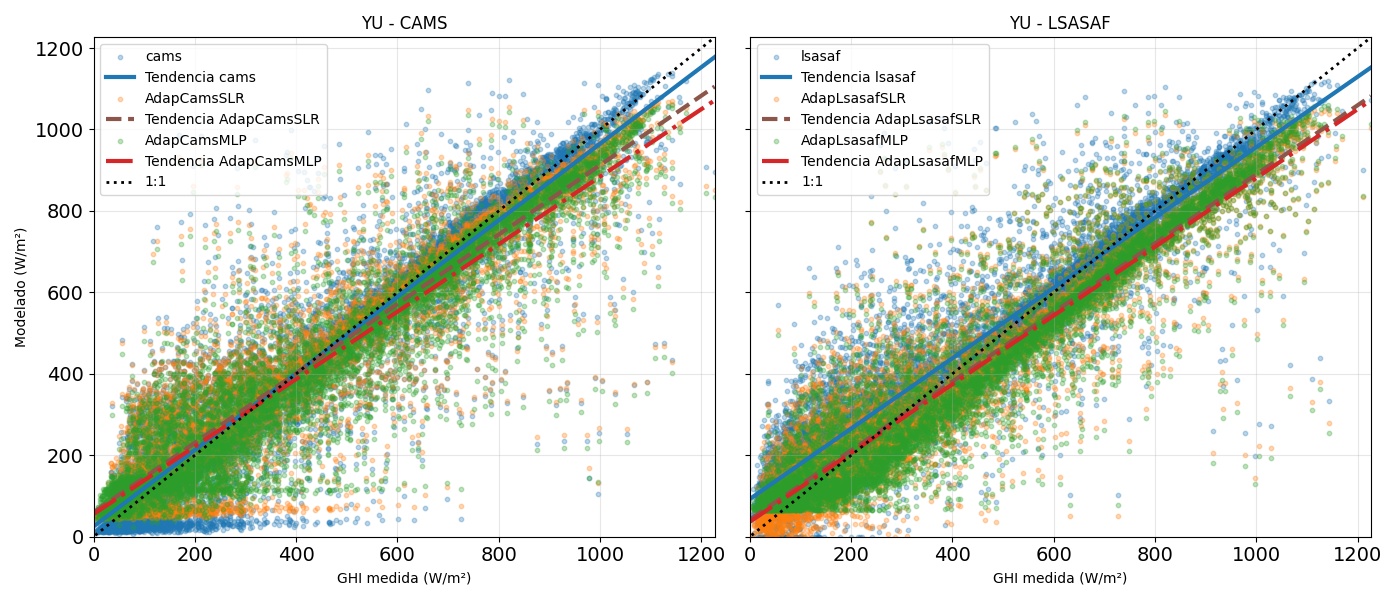
\includegraphics[width=0.9\textwidth]{figuras/scatter_yu_1.png}
%DIFDELCMD <     %%%
%DIFDELCMD < \caption{%
{%DIFAUXCMD
\DIFdelFL{Comparación de modelos CAMS y LSASAF y las adaptaciones con SLR y MLP en Yuto.}}
    %DIFAUXCMD
%DIFDELCMD < \label{fig:scatter-yu-01}
%DIFDELCMD < \end{figure}
%DIFDELCMD < 

%DIFDELCMD < %%%
\DIFdel{En Yu puede observarse que las nubes de puntos siguen de cerca la línea 1:1 y las tendencias adaptadas se solapan prácticamente con ella, mostrando un ajuste sobresaliente. Esto sugiere que en YU los productos satelitales capturan bien la variabilidad local de la irradiancia, por lo que la adaptación ofrece refinamientos marginales más que correcciones estructurales. 
}%DIFDELCMD < 

%DIFDELCMD < \begin{figure}
%DIFDELCMD <     \centering
%DIFDELCMD <     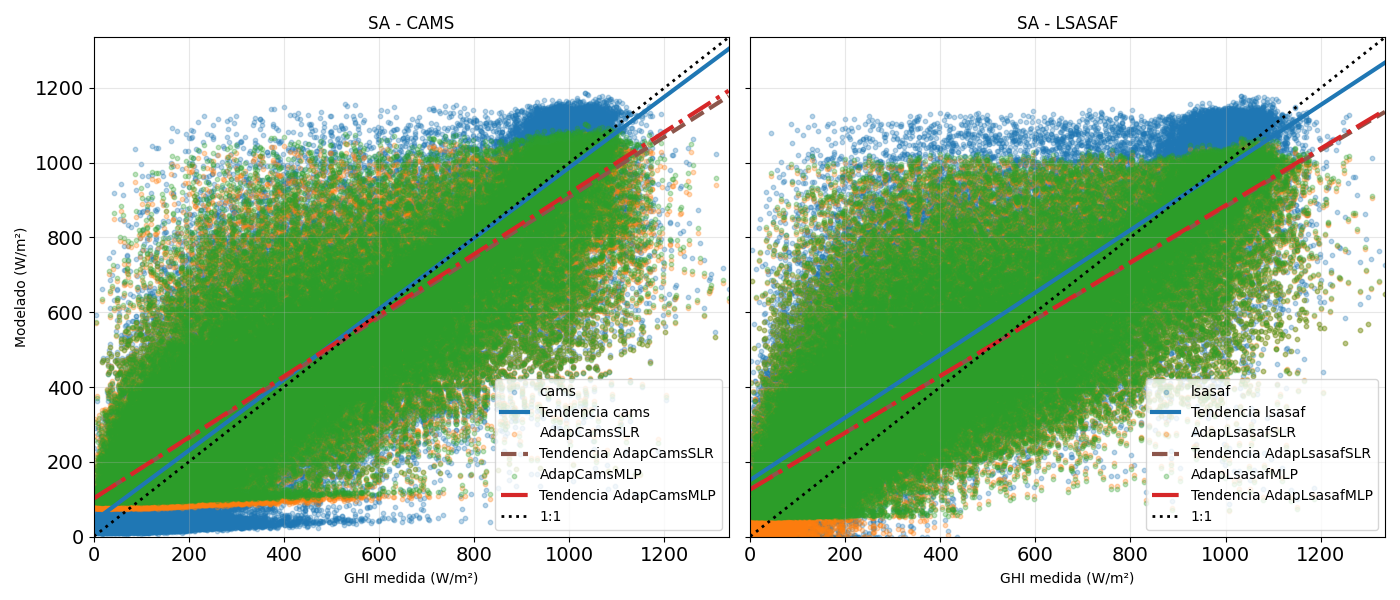
\includegraphics[width=0.9\textwidth]{figuras/scatter_sa_1.png}
%DIFDELCMD <     %%%
%DIFDELCMD < \caption{%
{%DIFAUXCMD
\DIFdelFL{Comparación de modelos CAMS y LSASAF y las adaptaciones con SLR Y MLP en Salta.}}
    %DIFAUXCMD
%DIFDELCMD < \label{fig:scatter-sa-01}
%DIFDELCMD < \end{figure}
%DIFDELCMD < 

%DIFDELCMD < %%%
\DIFdel{El sitio Sa presenta una mayor complejidad. Se observa una subestimación pronunciada en los modelos sin adaptar, especialmente en los valores altos de irradiancia, donde CAMS tiende a saturarse. Las adaptaciones corrigen parcialmente este sesgo, acercando las tendencias a la línea ideal. Aun así, la dispersión sigue siendo notable, indicando que las condiciones atmosféricas locales probablemente dificultan la modelización directa. Las métricas de la Tabla \ref{tab:metrics-as-1} reflejan esto. En general, la corrección estadística mitiga el sesgo pero no elimina la alta variabilidad del error, lo que sugiere limitaciones estructurales en la estimación satelital sobre esta zona.
}%DIFDELCMD < 

%DIFDELCMD < \begin{figure}
%DIFDELCMD <     \centering
%DIFDELCMD <     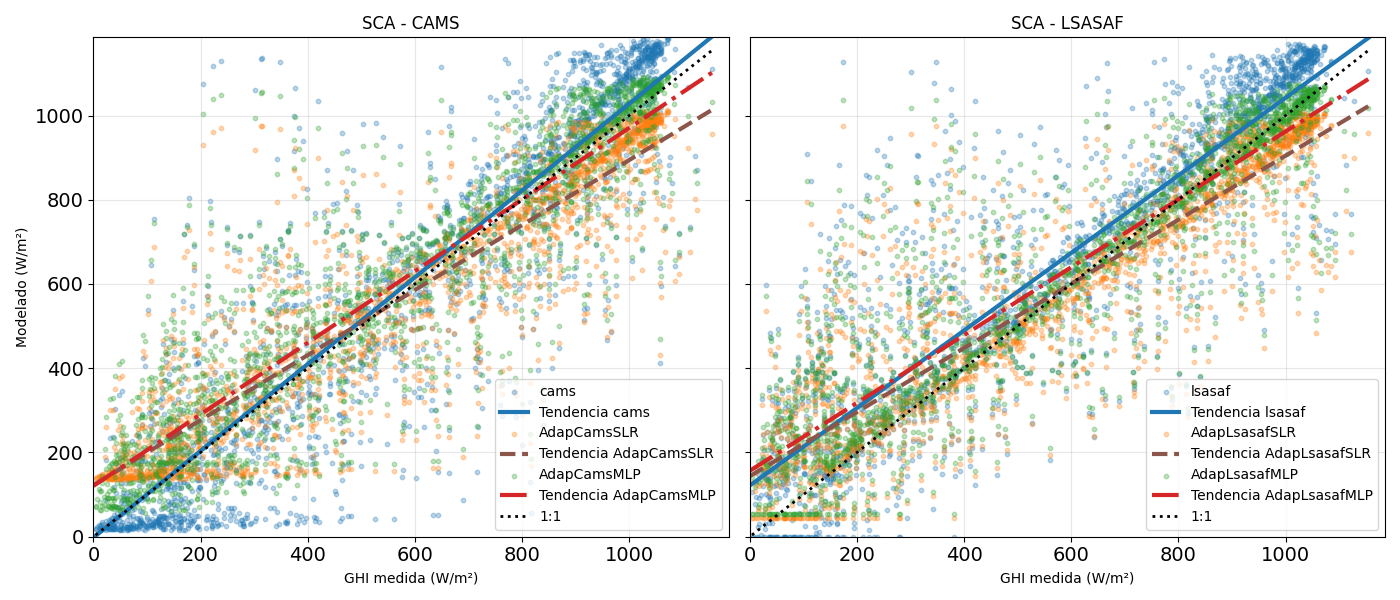
\includegraphics[width=0.9\textwidth]{figuras/scatter_sca_1.png}
%DIFDELCMD <     %%%
%DIFDELCMD < \caption{%
{%DIFAUXCMD
\DIFdelFL{Comparación de modelos CAMS y LSASAF y las adaptaciones con SLR y MLP en San Carlos.}}
    %DIFAUXCMD
%DIFDELCMD < \label{fig:scatter-sca-01}
%DIFDELCMD < \end{figure}
%DIFDELCMD < 

%DIFDELCMD < %%%
\DIFdel{En Ero, observa una alta subestimación por parte de CAMS y una ligera sobreestimación en LSA-SAF. La tendencia de los nuevamente la tendencia de los modelos modelos adaptados se acerca más a la línea 1:1, lo que indica una mejora significativa en la representación de los valores observados. Esto concuerda con las métricas: el RMSE disminuye de 40.9\% (CAMS) y 26.5\% (LSA-SAF) a alrededor de 31\% y 25\%, respectivamente, tras la adaptación. En conjunto, se evidencia el potencial del proceso de adaptación al sitio.
}%DIFDELCMD < 

%DIFDELCMD < \begin{figure}
%DIFDELCMD <     \centering
%DIFDELCMD <     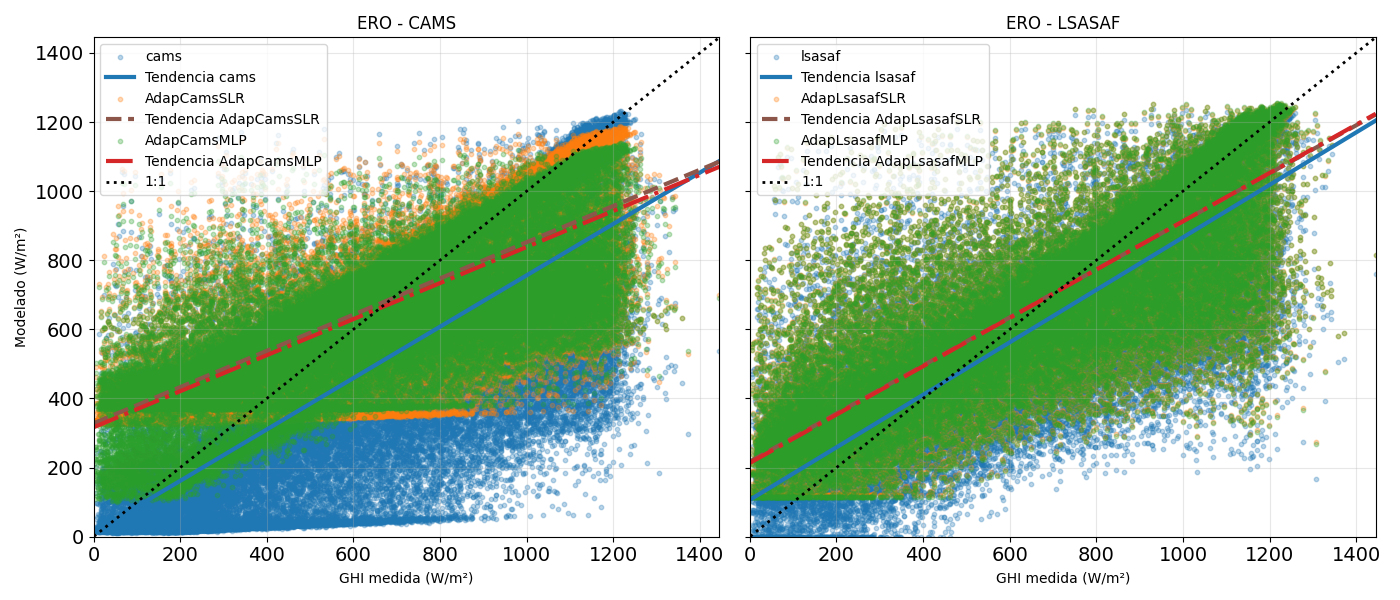
\includegraphics[width=0.9\textwidth]{figuras/scatter_ero_1.png}
%DIFDELCMD <     %%%
%DIFDELCMD < \caption{%
{%DIFAUXCMD
\DIFdelFL{Comparación de modelos CAMS y LSASAF y las adaptaciones con SLR y MLP en El Rosal.}}	
    %DIFAUXCMD
%DIFDELCMD < \label{fig:scatter-ero-01}
%DIFDELCMD < \end{figure}
%DIFDELCMD < 

%DIFDELCMD < %%%
\DIFdel{En Lq, se aprecia un comportamiento notablemente más ajustado para todos los modelos. Tanto CAMS como LSA-SAF muestran nubes de puntos más concentradas a lo largo de la línea 1:1, y las líneas de tendencia adaptadas prácticamente se superponen a ella. Los modelos sin adaptar ya presentaban un desempeño razonablemente bueno (RMSE de 25.8\% para CAMS y 22.6\% para LSA-SAF), pero las adaptaciones logran mejoras adicionales, alcanzando valores en torno a 23.5\% y 22\%. La homogeneidad y baja dispersión en el scatter sugieren una estabilidad radiativa del sitio y una alta representatividad de los datos satelitales, lo que explica la pequeña ganancia adicional obtenida mediante adaptación.
}%DIFDELCMD < 

%DIFDELCMD < \begin{figure}
%DIFDELCMD <     \centering
%DIFDELCMD <     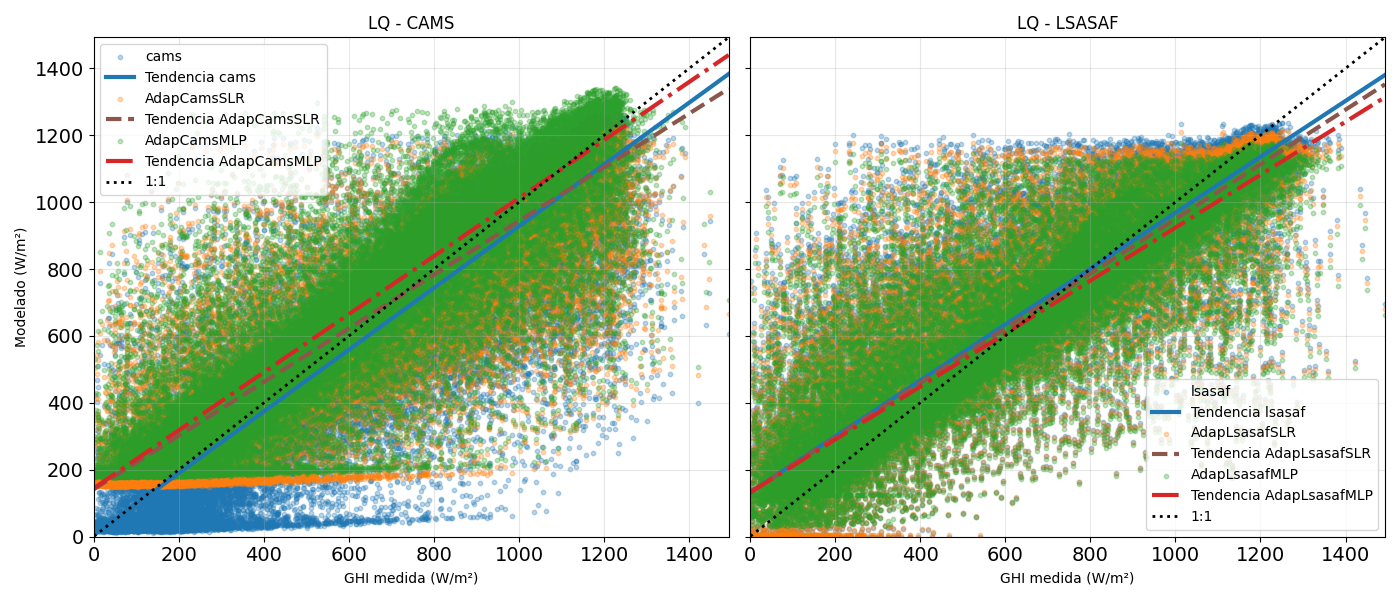
\includegraphics[width=0.9\textwidth]{figuras/scatter_lq_1.png}
%DIFDELCMD <     %%%
%DIFDELCMD < \caption{%
{%DIFAUXCMD
\DIFdelFL{Comparación de modelos CAMS y LSASAF y las adaptaciones con SLR y MLP en La Quiaca.}}
    %DIFAUXCMD
%DIFDELCMD < \label{fig:scatter-lq-01}
%DIFDELCMD < \end{figure}
%DIFDELCMD < 

%DIFDELCMD < %%%
\DIFdel{La Figura \ref{fig:mejorModelo} presenta las variaciones del rRMSE en cada sitio considerando el mejor desemepeño obtenido (menor rRMSE). Puede notarse que las ganancias sobre el desempeño podrían considerarse marginales, sin embargo sería interesante considerar el impacto que podria tener una variación del 3\% en la estimación del recurso solar, por ejemplo en la aplicación práctica. }%DIFDELCMD < \\
%DIFDELCMD < \begin{figure}
%DIFDELCMD <     \centering
%DIFDELCMD <     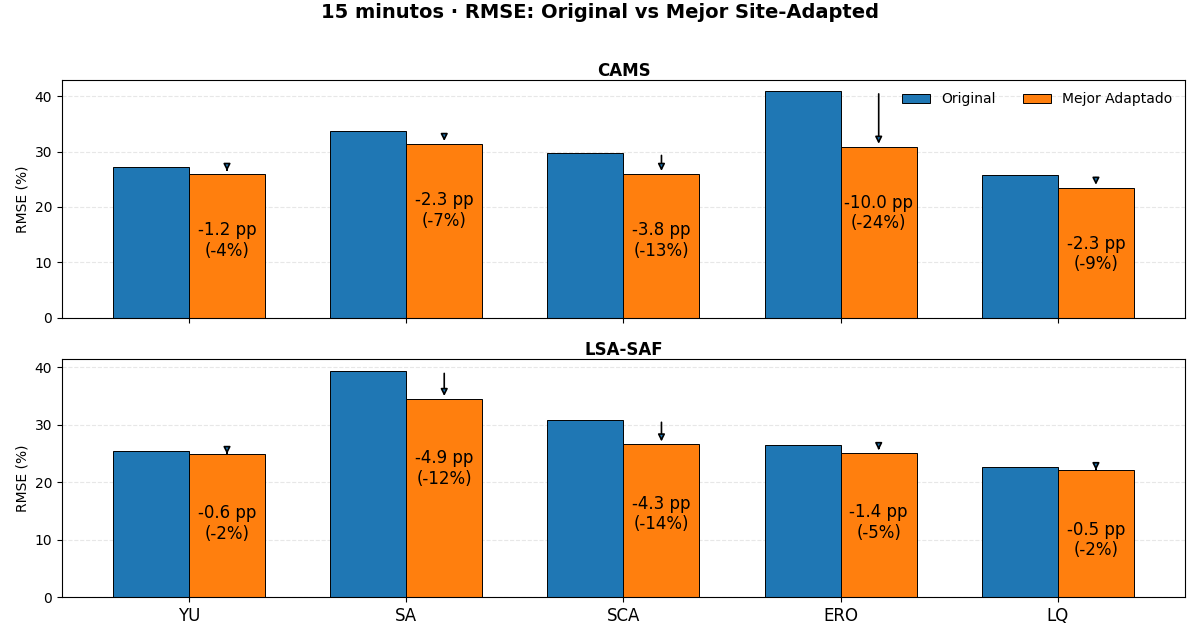
\includegraphics[width=0.9\textwidth]{figuras/comparativasRMSE15.png}
%DIFDELCMD <     %%%
%DIFDELCMD < \caption{%
{%DIFAUXCMD
\DIFdelFL{Comparación del rRMSE(\%) para los modelos crudos y el mejor desempeño obtenido.}}
    %DIFAUXCMD
%DIFDELCMD < \label{fig:mejorModelo}
%DIFDELCMD < \end{figure}
%DIFDELCMD < 

%DIFDELCMD < \begin{figure}
%DIFDELCMD <     \centering
%DIFDELCMD <     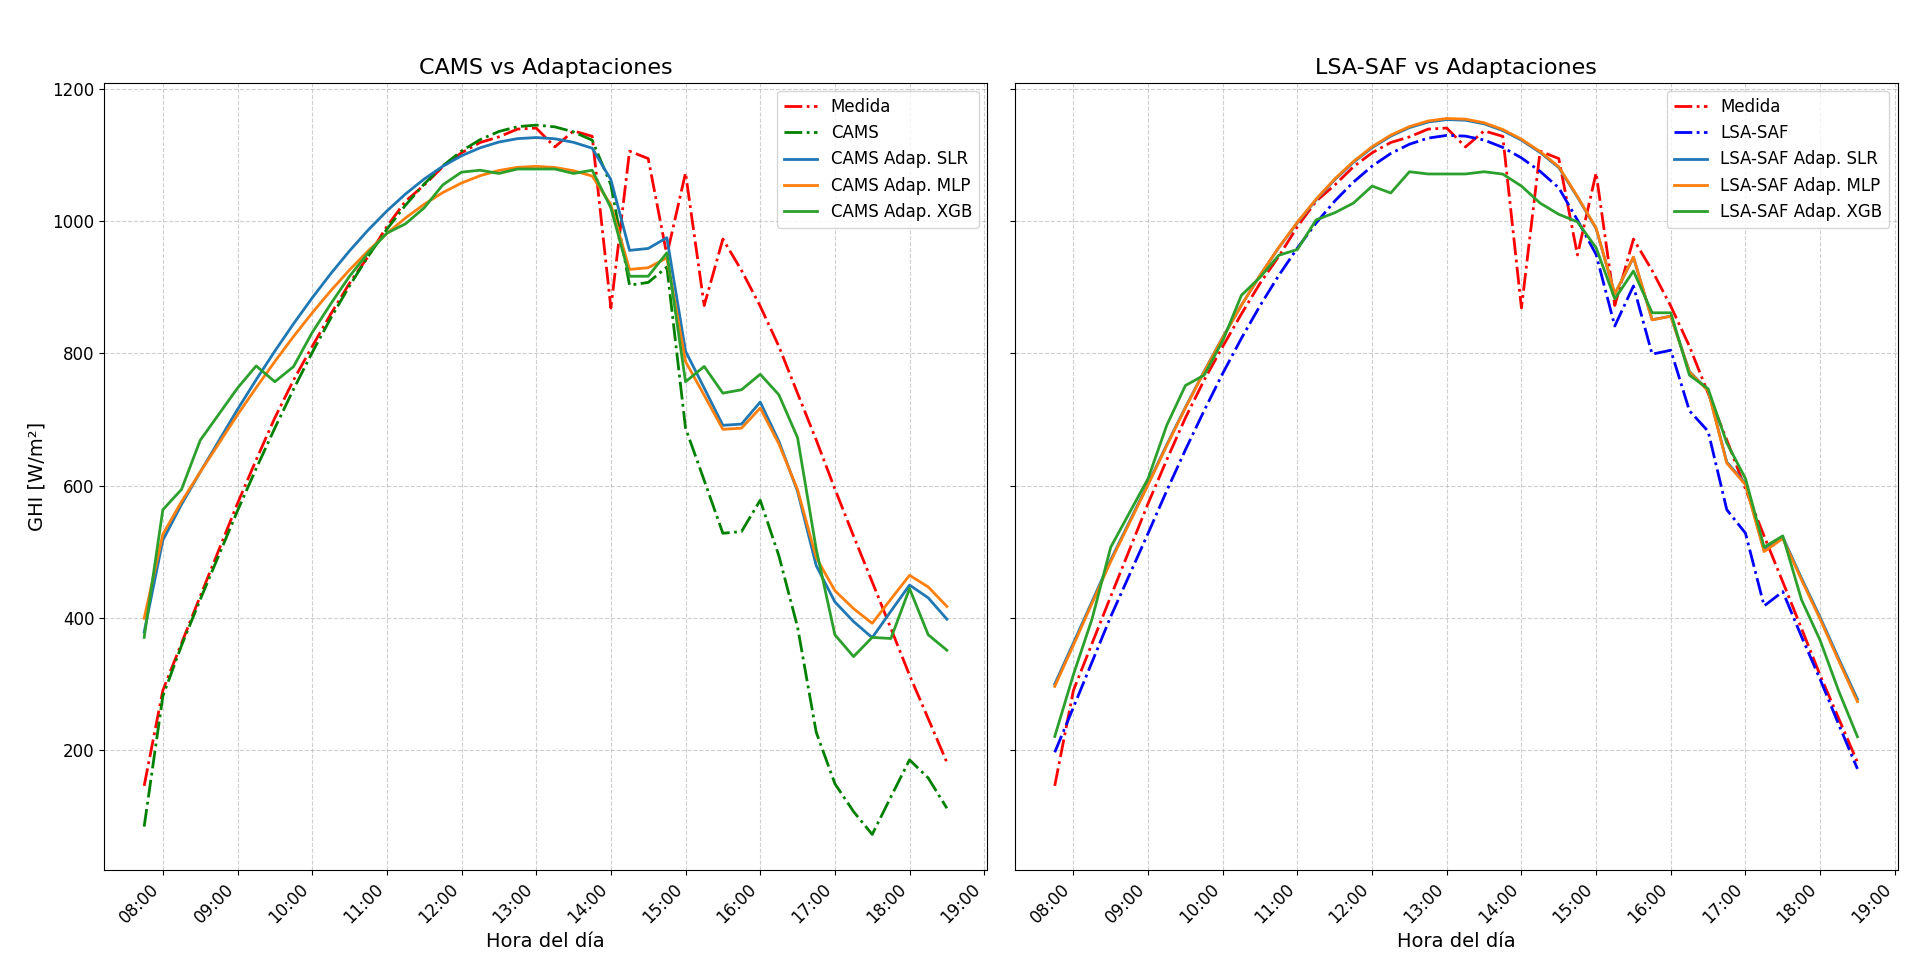
\includegraphics[width=0.95\textwidth]{figuras/AdaptacionEro1.png}
%DIFDELCMD <     %%%
%DIFDELCMD < \caption[Comparación del comportamiento de la GHI medida y estimada mediante los modelos CAMS y LSA-SAF, junto con sus respectivas adaptaciones basadas en los métodos SLR, MLP y XGB.]{%
{%DIFAUXCMD
\DIFdelFL{Comparación del comportamiento de la irradiancia global horizontal (GHI) medida y estimada mediante los modelos CAMS y LSA-SAF, junto con sus respectivas adaptaciones basadas en los métodos SLR, MLP y XGB, para la estación ERO el día 12 de octubre de 2016. Se observa que las adaptaciones mejoran el ajuste con respecto a la medición, especialmente durante las horas de máxima irradiancia.}}
    %DIFAUXCMD
%DIFDELCMD < \label{fig:adaptacionero}
%DIFDELCMD < \end{figure}
%DIFDELCMD < 

%DIFDELCMD < %%%
\DIFdel{La Figura \ref{fig:adaptacionero} muestra la evolución diaria de la irradiancia global horizontal (GHI) medida en superficie, junto con las estimaciones obtenidas a partir de los modelos satelitales CAMS y LSA-SAF, y sus respectivas adaptaciones mediante los métodos SLR, MLP y XGB, para el sitio ERO el 12 de octubre de 2016.
}%DIFDELCMD < 

%DIFDELCMD < %%%
\DIFdel{En el caso del modelo CAMS (panel izquierdo), se observa que la estimación original tiende a subestimar la irradiancia durante las primeras y últimas horas del día, mientras que presenta una ligera sobreestimación en torno al mediodía. Las adaptaciones basadas en SLR, MLP y XGB reducen significativamente dichas desviaciones, siendo las versiones MLP y XGB las que muestran la mayor concordancia con la medición. Estas últimas reproducen de manera casi exacta la forma y magnitud del ciclo diario, lo que sugiere que los modelos no lineales poseen una mayor capacidad para capturar las variaciones locales del recurso solar y corregir sesgos sistemáticos inherentes al modelo satelital.
}%DIFDELCMD < 

%DIFDELCMD < %%%
\DIFdel{En el modelo LSA-SAF (panel derecho), la versión original presenta un comportamiento más próximo a la medición que el modelo CAMS, particularmente durante las horas de máxima irradiancia. Sin embargo, se mantienen pequeñas sobreestimaciones hacia el final de la tarde. Las adaptaciones aplicadas, especialmente las obtenidas mediante MLP y XGB, mejoran notablemente el ajuste con respecto a la medición, reproduciendo de forma precisa tanto la amplitud como la estructura temporal del GHI observado.
}%DIFDELCMD < 

%DIFDELCMD < %%%
\DIFdel{En ambos modelos, las adaptaciones locales aportan una mejora sustancial en la representación del recurso solar en el sitio, lo que evidencia la utilidad de aplicar modelos de corrección calibrados con datos in situ. En síntesis, las adaptaciones mediante SLR, MLP y XGB preservan la forma física del ciclo diario de irradiancia y ajustan de manera adecuada la magnitud y tendencia de los valores estimados. Esto sugiere que, en sitios con predominancia de condiciones de cielo claro, las metodologías de adaptación poseen un alto potencial para reducir los errores sistemáticos en las estimaciones de irradiancia derivadas de modelos satelitales, contribuyendo así a una mejor caracterización local del recurso solar.
}%DIFDELCMD < 

%DIFDELCMD < %%%
\DIFdel{Los resultados de este análisis inicial indican que, en el contexto de la adaptación de modelos satelitales para estimación de GHI, los métodos de aprendizaje automático evaluados (SLR, XGB y MLP) presentan rendimientos comparables en términos de métricas de error estándar, con diferencias relativamente pequeñas entre ellos. A pesar de su simplicidad, el modelo SLR demostró una capacidad notable para capturar la relación entre los datos satelitales y las mediciones terrestres, alcanzando niveles de error relativos similares a los obtenidos por los modelos más complejos (XGB y MLP).
}%DIFDELCMD < 

%DIFDELCMD < %%%
\DIFdel{Este comportamiento podría deberse a que la calidad de los datos de entrada impone un límite superior a la precisión alcanzable por los modelos más sofisticados. Los productos satelitales utilizados presentan incertidumbres inherentes y limitaciones en su resolución temporal y espacial, lo que restringe su capacidad para representar fenómenos de alta frecuencia o de origen local, como los efectos microclimáticos o la variabilidad inducida por el relieve. En consecuencia, aumentar la complejidad del modelo no necesariamente se traduce en una mejora sustancial del rendimiento predictivo bajo estas condiciones de datos.
}%DIFDELCMD < 

%DIFDELCMD < %%%
\DIFdel{Por otra parte, se observó que los modelos más flexibles, como el MLP, pueden ser susceptibles al sobreajuste, lo cual se refleja en un comportamiento menos consistente entre las distintas métricas de desempeño. Esto resalta la necesidad de equilibrar la complejidad del modelo con la calidad y cantidad de datos disponibles, a fin de preservar la capacidad de generalización. En este sentido, y dadas las características actuales de los datos y del sitio, modelos más simples como el SLR constituyen una alternativa robusta, interpretable y computacionalmente eficiente para la estimación adaptada del GHI.
}%DIFDELCMD < 

%DIFDELCMD < %%%
\DIFdel{En el futuro, las mejoras más significativas en precisión probablemente se lograrán mediante la incorporación de variables meteorológicas adicionales, la aplicación de técnicas de descomposición temporal o el desarrollo de enfoques híbridos que combinen modelos físicos con correcciones estadísticas, más que mediante el simple incremento de la complejidad algorítmica.
}%DIFDELCMD < 

%DIFDELCMD < %%%
\DIFdel{Finalmente, se observó que las ganancias en desempeño que aportan las técnicas de regresión son más pronunciadas en los casos donde la combinación sitio–modelo de estimación presenta inicialmente un bajo desempeño. Esto podría explicarse porque existe un mayor margen de mejora en esos contextos. Por el contrario, en las combinaciones sitio–modelo donde las estimaciones originales ya son adecuadas, la mejora aportada por la adaptación resulta más marginal, lo cual concuerda con lo reportado en trabajos previos de \citet{SALAMALIKIS2022, POLO2020}.
}%DIFDELCMD < 

%DIFDELCMD < %%%
\section{\DIFdel{Adaptación al sitio con múltiples variables descriptivas}}%DIFAUXCMD
\addtocounter{section}{-1}%DIFAUXCMD
%DIFDELCMD < \label{sec:02}
%DIFDELCMD < 

%DIFDELCMD < %%%
\DIFdel{En la sección anterior se presentaron los resultados del proceso de adaptación al sitio utilizando un enfoque tradicional basado en mejorar la estimación de un modelo a partir de la variable propiamente modelada y de mediciones in situ. Este enfoque se centra en la relación directa entre la variable objetivo y sus observaciones. Sin embargo, en los últimos años se ha desarrollado una estrategia más avanzada que consiste en incorporar variables regresoras adicionales durante el entrenamiento de los modelos de regresión. La idea subyacente es que estas variables pueden aportar información complementaria, potencialmente mejorando la precisión de la estimación en comparación con un enfoque que utiliza únicamente la variable principal. 
}%DIFDELCMD < 

%DIFDELCMD < %%%
\DIFdel{En la práctica, estas variables adicionales pueden provenir de distintos modelos de reanálisis o de fuentes satelitales, y se seleccionan bajo la expectativa de que estén correlacionadas, de alguna manera, con la irradiancia global horizontal (GHI) medida. Este enfoque ha sido aplicado y documentado en trabajos previos, como \cite{Salazar2025, Miranda2021, Miranda2023}.
}%DIFDELCMD < 

%DIFDELCMD < %%%
\DIFdel{La ampliación del conjunto de regresores y la automatización del proceso de entrenamiento resulta especialmente atractiva considerando que los modelos de aprendizaje automático se utilizan cada vez más para identificar patrones y extraer información de grandes volúmenes de datos. No obstante, la efectividad de estos modelos depende en gran medida de la calidad y relevancia de los regresores empleados: no basta con añadir más variables, estas deben ser apropiadas y contener información útil para la tarea de predicción.
}%DIFDELCMD < 

%DIFDELCMD < %%%
\subsection{\DIFdel{La necesidad de un análisis exploratorio de datos}}
%DIFAUXCMD
\addtocounter{subsection}{-1}%DIFAUXCMD
%DIFDELCMD < 

%DIFDELCMD < %%%
\DIFdel{Antes de implementar la adaptación con todos los regresores disponibles, es fundamental realizar un análisis exploratorio de datos (AED). Este paso se puede comparar con inspeccionar un terreno antes de construir una casa: si no conocemos la distribución del terreno, la presencia de obstáculos o la estabilidad del suelo, cualquier construcción posterior podría ser ineficiente o incluso fallar. De manera análoga, un AED permite comprender las características básicas de cada variable, su rango, posibles valores atípicos, correlaciones y relaciones con la variable objetivo, asegurando que el modelo posterior tenga una base sólida.  
}%DIFDELCMD < 

%DIFDELCMD < %%%
\DIFdel{El AED no solo ayuda a identificar qué variables pueden ser más relevantes, sino que también sirve para detectar problemas en ellas, como valores faltantes, inconsistencias o errores de modelado, que podrían afectar la calidad de la estimación \citep{Tukey1977, Behrens1997, Wilks2006}. Por ejemplo, variables mal calculadas o extremadamente ruidosas podrían introducir sesgos en el modelo de regresión, reduciendo su capacidad de generalización. Comprender estos aspectos antes de la construcción del modelo es crucial para asegurar que los resultados sean confiables y reproducibles.  
}%DIFDELCMD < 

%DIFDELCMD < %%%
\DIFdel{Además, el AED permite evaluar relaciones no lineales y patrones temporales que podrían no ser evidentes a simple vista. Por ejemplo, la relación entre la irradiancia solar y la temperatura o la humedad puede variar a lo largo del año, y detectar estos patrones ayuda a definir qué regresores son realmente útiles \citep{ Kuhn2013}. Esta exploración es especialmente importante cuando se dispone de un gran número de variables regresoras, porque es probable que no todas aportaran información significativa.  
}%DIFDELCMD < 

%DIFDELCMD < %%%
\DIFdel{Finalmente, realizar un AED exhaustivo permite planificar estrategias de reducción de dimensionalidad o selección de variables antes de aplicar modelos complejos. En este trabajo, se propone inicialmente realizar la adaptación del modelo utilizando todos los regresores disponibles para obtener una estimación completa. Posteriormente, se utilizarán los resultados del AED para identificar los regresores más relevantes y comparar su desempeño con el modelo completo. Este enfoque dual combina la riqueza de información disponible con la eficiencia y robustez que aporta un conjunto de variables cuidadosamente seleccionado.  
}%DIFDELCMD < 

%DIFDELCMD < %%%
\subsection{\DIFdel{Implementación de la adaptación con múltiples regresores}}
%DIFAUXCMD
\addtocounter{subsection}{-1}%DIFAUXCMD
%DIFDELCMD < 

%DIFDELCMD < %%%
\DIFdel{En la sección anterior, el proceso de adaptación al sitio se definía mediante la siguiente expresión:
}%DIFDELCMD < 

%DIFDELCMD < %%%
\begin{displaymath}
\DIFdel{GHI_{adaptado} = ML_{Regresor}(GHI_{modelado}),
%DIFDELCMD < \label{ec:SiteAdapSimple}%%%
}\end{displaymath}%DIFAUXCMD
%DIFDELCMD < 

%DIFDELCMD < \noindent %%%
\DIFdel{donde $ML_{Regresor}$ representa cualquiera de los modelos de regresión utilizados (SLR, MLP o XGB). 
}%DIFDELCMD < 

%DIFDELCMD < %%%
\DIFdel{En esta sección se propone incrementar el conjunto de variables regresoras, con la expectativa de que estas aporten información adicional al modelo de regresión. De este modo, la alternativa para la adaptación puede expresarse como:
}%DIFDELCMD < 

%DIFDELCMD < %%%
\begin{displaymath}
\DIFdel{GHI_{adaptado} = ML_{Regresor}(Reg_{1}, Reg_{2}, Reg_{3},..., Reg_{n}),
%DIFDELCMD < \label{ec:SiteAdapMultiple}%%%
}\end{displaymath}%DIFAUXCMD
%DIFDELCMD < 

%DIFDELCMD < \noindent %%%
\DIFdel{donde cada $Reg_{i}$ representa una variable regresora; incluyendo $GHI_{modelado}$, que también forma parte del conjunto.
}%DIFDELCMD < 

%DIFDELCMD < %%%
\DIFdel{Para este trabajo se propuso un conjunto de variables de carácter astronómico, atmosférico y meteorológico, definidas de la siguiente manera:
}%DIFDELCMD < 

%DIFDELCMD < \begin{itemize}
\begin{itemize}%DIFAUXCMD
%DIFDELCMD < \item %%%
\item%DIFAUXCMD
\DIFdel{\texttt{N}: Día del año.
}%DIFDELCMD < \item %%%
\item%DIFAUXCMD
\DIFdel{\texttt{SZA}: Ángulo cenital solar.
}%DIFDELCMD < \item %%%
\item%DIFAUXCMD
\DIFdel{\texttt{$\alpha$}: Altura solar.
}%DIFDELCMD < \item %%%
\item%DIFAUXCMD
\DIFdel{\texttt{TOA}: Irradiancia en la parte superior de la atmósfera.
}%DIFDELCMD < \item %%%
\item%DIFAUXCMD
\DIFdel{\texttt{GHIargp2}: Irradiancia bajo cielo despejado según \cite{Ledesma2023a}.
}%DIFDELCMD < \item %%%
\item%DIFAUXCMD
\DIFdel{\texttt{delta}: Declinación solar.
}%DIFDELCMD < \item %%%
\item%DIFAUXCMD
\DIFdel{\texttt{Fn}: Función normalizada de duración del día.
}%DIFDELCMD < \item %%%
\item%DIFAUXCMD
\DIFdel{\texttt{E0}: Factor de corrección extraterrestre.
}%DIFDELCMD < \item %%%
\item%DIFAUXCMD
\DIFdel{\texttt{mr}: Masa de aire relativa \cite{Gueymard2003}.
}%DIFDELCMD < \item %%%
\item%DIFAUXCMD
\DIFdel{\texttt{tm}: Temperatura media del aire según ERA5.
}%DIFDELCMD < \item %%%
\item%DIFAUXCMD
\DIFdel{\texttt{uw}: Componente U del viento según ERA5.
}%DIFDELCMD < \item %%%
\item%DIFAUXCMD
\DIFdel{\texttt{dw}: Componente V del viento según ERA5.
}%DIFDELCMD < \item %%%
\item%DIFAUXCMD
\DIFdel{\texttt{tcw}: Vapor de agua total en la columna atmosférica según ERA5.
}%DIFDELCMD < \item %%%
\item%DIFAUXCMD
\DIFdel{\texttt{2mdt}: Temperatura del punto de rocío a 2 metros sobre el suelo según ERA5.
}%DIFDELCMD < 


\end{itemize}%DIFAUXCMD
%DIFDELCMD < \end{itemize}
%DIFDELCMD < 

%DIFDELCMD < %%%
\DIFdel{Las variables \texttt{tm}, \texttt{uw}, \texttt{dw} y \texttt{2mdt} provienen del modelo ERA5 y se encuentran disponibles a escala horaria. Por esta razón, consideramos inapropiado interpolarlas a una resolución de 15 minutos, ya que esta transformación no añade información real y podría introducir errores. En consecuencia, las evaluaciones presentadas en esta sección se realizan exclusivamente a escala horaria.
}%DIFDELCMD < 

%DIFDELCMD < %%%
\DIFdel{Aunque, desde un punto de vista técnico, es posible interpolar estas variables para obtener valores a intervalos menores, el resultado dependería más del método de interpolación que de las características físicas del sitio o del proceso de adaptación del modelo. Mantener la escala temporal original garantiza así una mayor consistencia y validez en el análisis.}%DIFDELCMD < \\
%DIFDELCMD < 

%DIFDELCMD < \begin{table*}[h]
%DIFDELCMD < %%%
%DIFDELCMD < \caption[Métricas de desempeño para cada modelo en el conjunto de pruebas. ]{%
{%DIFAUXCMD
\DIFdelFL{Métricas de desempeño (MBE, MAE, RMSE) para cada modelo en el conjunto de pruebas de los cinco sitios. Los valores están normalizados y expresados como porcentajes relativos a la media de GHI en cada sitio: 429.2~W/m$^2$ (Yu), 432.9~W/m$^2$ (Sa), 554.4~W/m$^2$ (Sca), 628.4~W/m$^2$ (Ero), y 648.7~W/m$^2$ (Lq). Los modelos etiquetados con ``(1 var.)'' indican adaptación al sitio realizada utilizando solo un regresor (CAMS o LSA-SAF).}}
%DIFAUXCMD
%DIFDELCMD < \label{tab:metricas_3_1}
%DIFDELCMD < \centering
%DIFDELCMD < \resizebox{\linewidth}{!}{
%DIFDELCMD < \def\arraystretch{1.5}
%DIFDELCMD < \begin{tabular}{cccccccccccccccc}
%DIFDELCMD < \hline
%DIFDELCMD <       & \multicolumn{3}{c}{Yu} & \multicolumn{3}{c}{Sa} & \multicolumn{3}{c}{Sca} & \multicolumn{3}{c}{Ero} & \multicolumn{3}{c}{Lq} \\
%DIFDELCMD < Modelo & MBE & MAE & RMSE & MBE & MAE & RMSE  & MBE & MAE & RMSE & MBE & MAE & RMSE & MBE & MAE & RMSE  \\
%DIFDELCMD < \hline
%DIFDELCMD < \multicolumn{16}{|c|}{\textit{Estimaciones satelitales en bruto}} \\
%DIFDELCMD < \hline
%DIFDELCMD < CAMS    & -0.1 & 15.2 & 23.5 & 4.0 & 20.9 & 29.3 & 3.0 & 19.7 & 26.1 & -23.6 & 26.6 & 39.3 & -4.8 & 14.5 & 21.6 \\
%DIFDELCMD < LSA-SAF & 7.5  & 14.4 & 21.8 & 17.9 & 25.3 & 35.7 & 13.3 & 20.3 & 27.1 & -7.7  & 14.8 & 24.0 & 4.8  & 10.9 & 18.2 \\
%DIFDELCMD < ERA5    & 1.2  & 22.2 & 33.7 & 9.4  & 27.1 & 37.7 & 1.9  & 20.2 & 29.7 & -14.0 & 19.3 & 25.6 & -0.8 & 11.3 & 18.4 \\
%DIFDELCMD < MERRA-2 & 24.9 & 33.5 & 51.2 & 43.4 & 48.3 & 65.0 & 10.9 & 21.7 & 30.3 & -3.8  & 13.1 & 20.4 & 1.4  & 13.4 & 20.8 \\
%DIFDELCMD < \hline
%DIFDELCMD < 

%DIFDELCMD < \multicolumn{16}{|c|}{\textit{Adaptación al sitio conjunto completo de regresores (15 vars.)}} \\
%DIFDELCMD < \hline
%DIFDELCMD < CAMS    MLR & -3.3 & 14.6 & 21.7 & 3.4 & 18.3 & 26.6 & 1.1 & 16.3 & 23.5 & 0.6 & 13   & 20 & 0.8 & 10.6 & 16.2 \\
%DIFDELCMD < CAMS    MLP & -2.8 & 13.9 & 20.9 & 3.5 & 18   & 26.3 & 3.6  & 16.8 & 24.3 & 0.3 & 13.3 & 20.2 &  0   & 10.8 & 16.1 \\
%DIFDELCMD < CAMS    XGB & -2.8 & 14.6 & 21.5 & 2.2 & 18.1 & 26.9 & -0.1 & 18.8 & 26.1 & 0.1 & 13.8 & 21.5 & 0.7 & 10.9 & 16.9 \\
%DIFDELCMD < \hline
%DIFDELCMD < LSA-SAF MLR & -4.9 & 14.4 & 20.7 & 3.9 & 21   & 29.9 & 0.2 & 18.5 & 25.2 & 0.9 & 12.2 & 19.2 & 0.1 & 11.4 & 17.1 \\
%DIFDELCMD < LSA-SAF MLP & -5.0 & 14.2 & 20.3 & 3.0 & 20.6 & 29.3 & 3.1  & 18.3 & 25.8 & 0.7 & 12.6 & 19.4 & -0.3 & 11.5 & 16.8 \\
%DIFDELCMD < LSA-SAF XGB& -4.1 & 14.7 & 21.1 & 2.6 & 21.2 & 30.5 & -1.1 & 21.2 & 29.3 & 0.4 & 13.1 & 20.5 & -0.1 & 11.6 & 17.5 \\
%DIFDELCMD < \hline
%DIFDELCMD < ERA5    MLR & -1.5 & 22.8 & 31.1 & 5.9 & 26.4 & 35.9 & -2.8 & 20  & 26.6 & -0.8& 12.9 & 19.4 & 0.4 & 10.9 & 17 \\
%DIFDELCMD < ERA5    MLP & -0.6 & 22.7 & 31.3 & 6.3 & 26.9 & 36   & -1.2 & 20.2 & 27.2 & -1  & 13.4 & 19.7 & -0.8 & 11.7 & 17.2 \\
%DIFDELCMD < ERA5    XGB & -0.2 & 24.1 & 32.9 & 4.0 & 26.8 & 37.1 & -3.4 & 23.3 & 31.7 & -1.0 & 13.7 & 20.9 & 0.3 & 11.9 & 18.6 \\
%DIFDELCMD < \hline
%DIFDELCMD < MERRA-2 MLR & -6.1 & 31.2 & 39.6 & 5.5 & 31.2 & 40.2 & -0.2 & 20.4& 27.7 & 0.7 & 12   & 19.0 & -0.2 & 12.1 & 18.2 \\
%DIFDELCMD < MERRA-2 MLP & -4.3 & 31.5 & 39.6 & 5.7 & 30.4 & 39.3 & 3    & 19.2 & 27.2 & 0.7 & 12.3 & 19.1 & -1.5 & 12.4 & 18  \\
%DIFDELCMD < MERRA-2 XGB & -4.4 & 31.1 & 39.7 & 4.4 & 29.8 & 40.0 & -0.8 & 22.1 & 30.3 & -0.1 & 13.3 & 20.7 & -0.6 & 12.4 & 18.5 \\
%DIFDELCMD < 

%DIFDELCMD < \hline
%DIFDELCMD < \end{tabular}}
%DIFDELCMD < \end{table*}
%DIFDELCMD < 

%DIFDELCMD < \begin{figure*}
%DIFDELCMD <     \centering
%DIFDELCMD <     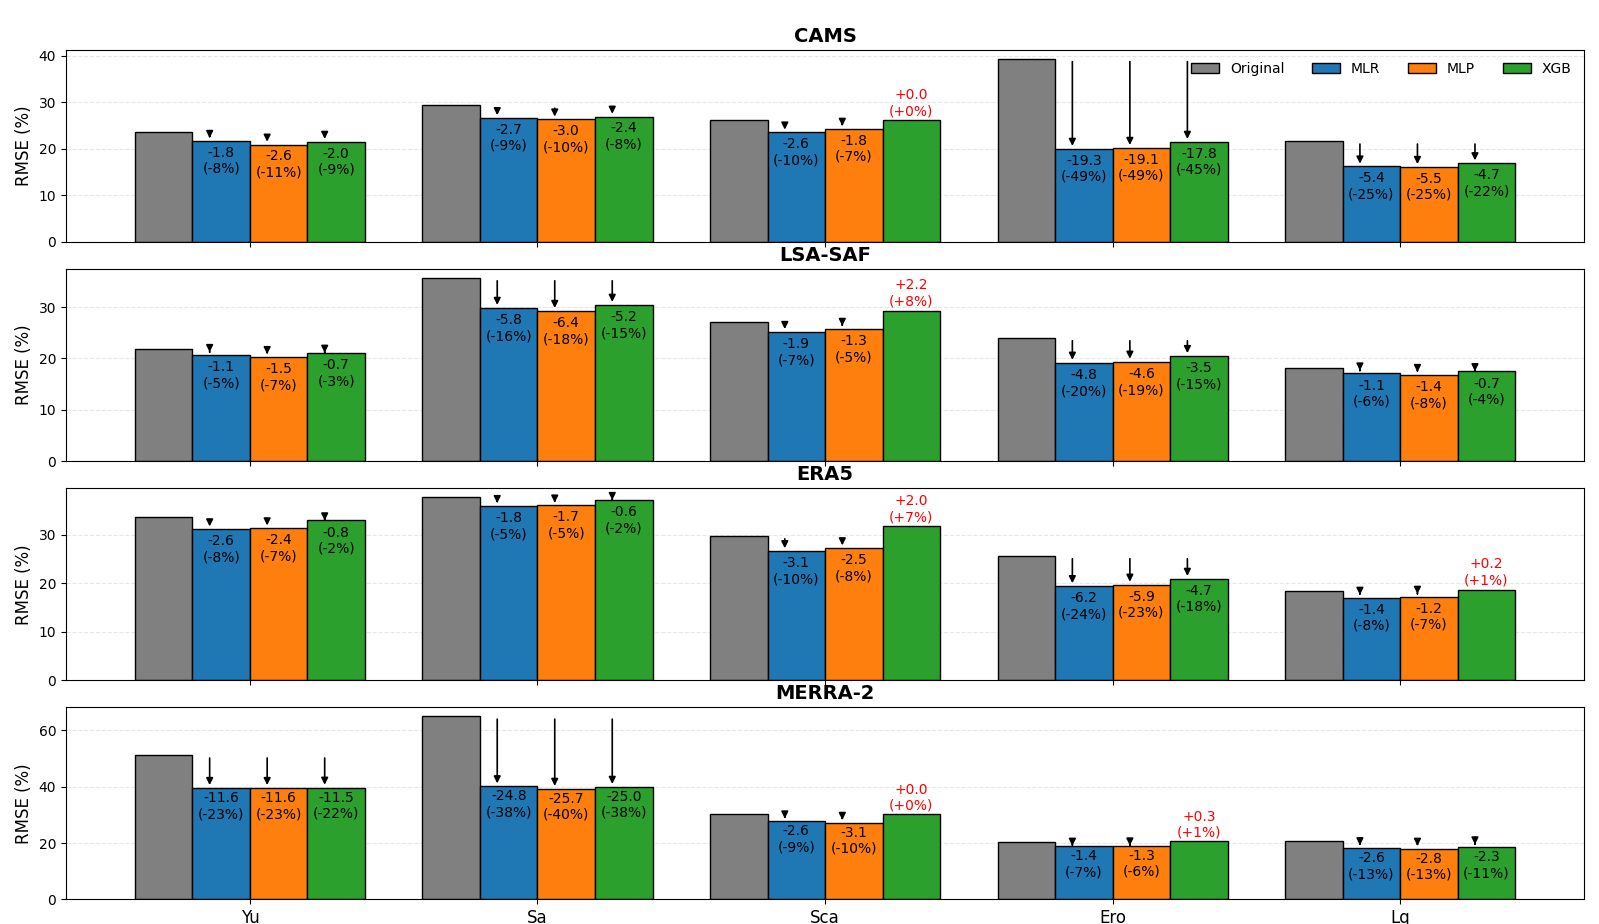
\includegraphics[width=\textwidth]{rmsd_full.png} 
%DIFDELCMD <     %%%
%DIFDELCMD < \caption[Comparación del rRMSE(\%) entre estimaciones originales de los satélites y sus versiones adaptadas.]{%
{%DIFAUXCMD
\DIFdelFL{Comparación del rRMSE(\%) entre estimaciones originales de los satélites y sus versiones adaptadas mediante los regresores MLR, MLP y XGB para los cinco sitios (Yu, Sa, Sca, Ero y Lq). Las flechas indican mejora en la métrica adaptada respecto al valor original; las anotaciones muestran el cambio absoluto y relativo. Las flechas negras representan mejoras, mientras que las flechas rojas indican empeoramiento del desempeño respecto al modelo original.}}
    %DIFAUXCMD
%DIFDELCMD < \label{fig:regressors_comparison}
%DIFDELCMD < \end{figure*}
%DIFDELCMD < 

%DIFDELCMD < %%%
\DIFdel{Los resultados de la Tabla \ref{tab:metricas_3_1} y la Figura \ref{fig:regressors_comparison} muestran que la mayoría de los modelos logran adaptarse con la misma consistencia en cada sitio. Sin embargo, se evidencian casos en los que la métrica aumenta (flechas rojas), lo que sugiere que ciertos modelos adaptados no generalizan correctamente en todos los sitios.
}%DIFDELCMD < 

%DIFDELCMD < %%%
\DIFdel{Entre los regresores evaluados, se observa que XGB y MLP no producen mejoras significativamente mayores que las obtenidas con MLR. Esto indica que, aunque los modelos regresores más sofisticados son capaces de capturar relaciones no lineales, es necesario un análisis previo que permita identificar qué variables tienen mayor potencial como regresores antes de introducirlas en el modelo.
}%DIFDELCMD < 

%DIFDELCMD < %%%
\DIFdel{Estos resultados preliminares subrayan la importancia de realizar un análisis exploratorio que permita determinar qué variables son más prometedoras para cada sitio y, de este modo, seleccionar un conjunto de regresores que garantice un desempeño consistente y robusto. En este sentido, la selección de características se convierte en un paso crítico del preprocesamiento al entrenar modelos de ML, ya que permite identificar las variables más relevantes y eliminar aquellas redundantes o irrelevantes \citep{liu2023, Huang2024}. Una selección adecuada de características mejora la interpretabilidad del modelo, optimiza su eficiencia computacional y aumenta su capacidad predictiva, mientras que la inclusión de variables irrelevantes puede inducir sobreajuste \citep{che2024a}. Si bien, métodos como los de filtro, envolventes y embebidos permiten automatizar este proceso, pero el análisis exploratorio de datos sigue siendo fundamental para guiar la selección inicial de regresores y variables \citep{Cheng2024}.
}%DIFDELCMD < 

%DIFDELCMD < \begin{figure*}
%DIFDELCMD <     \centering
%DIFDELCMD <     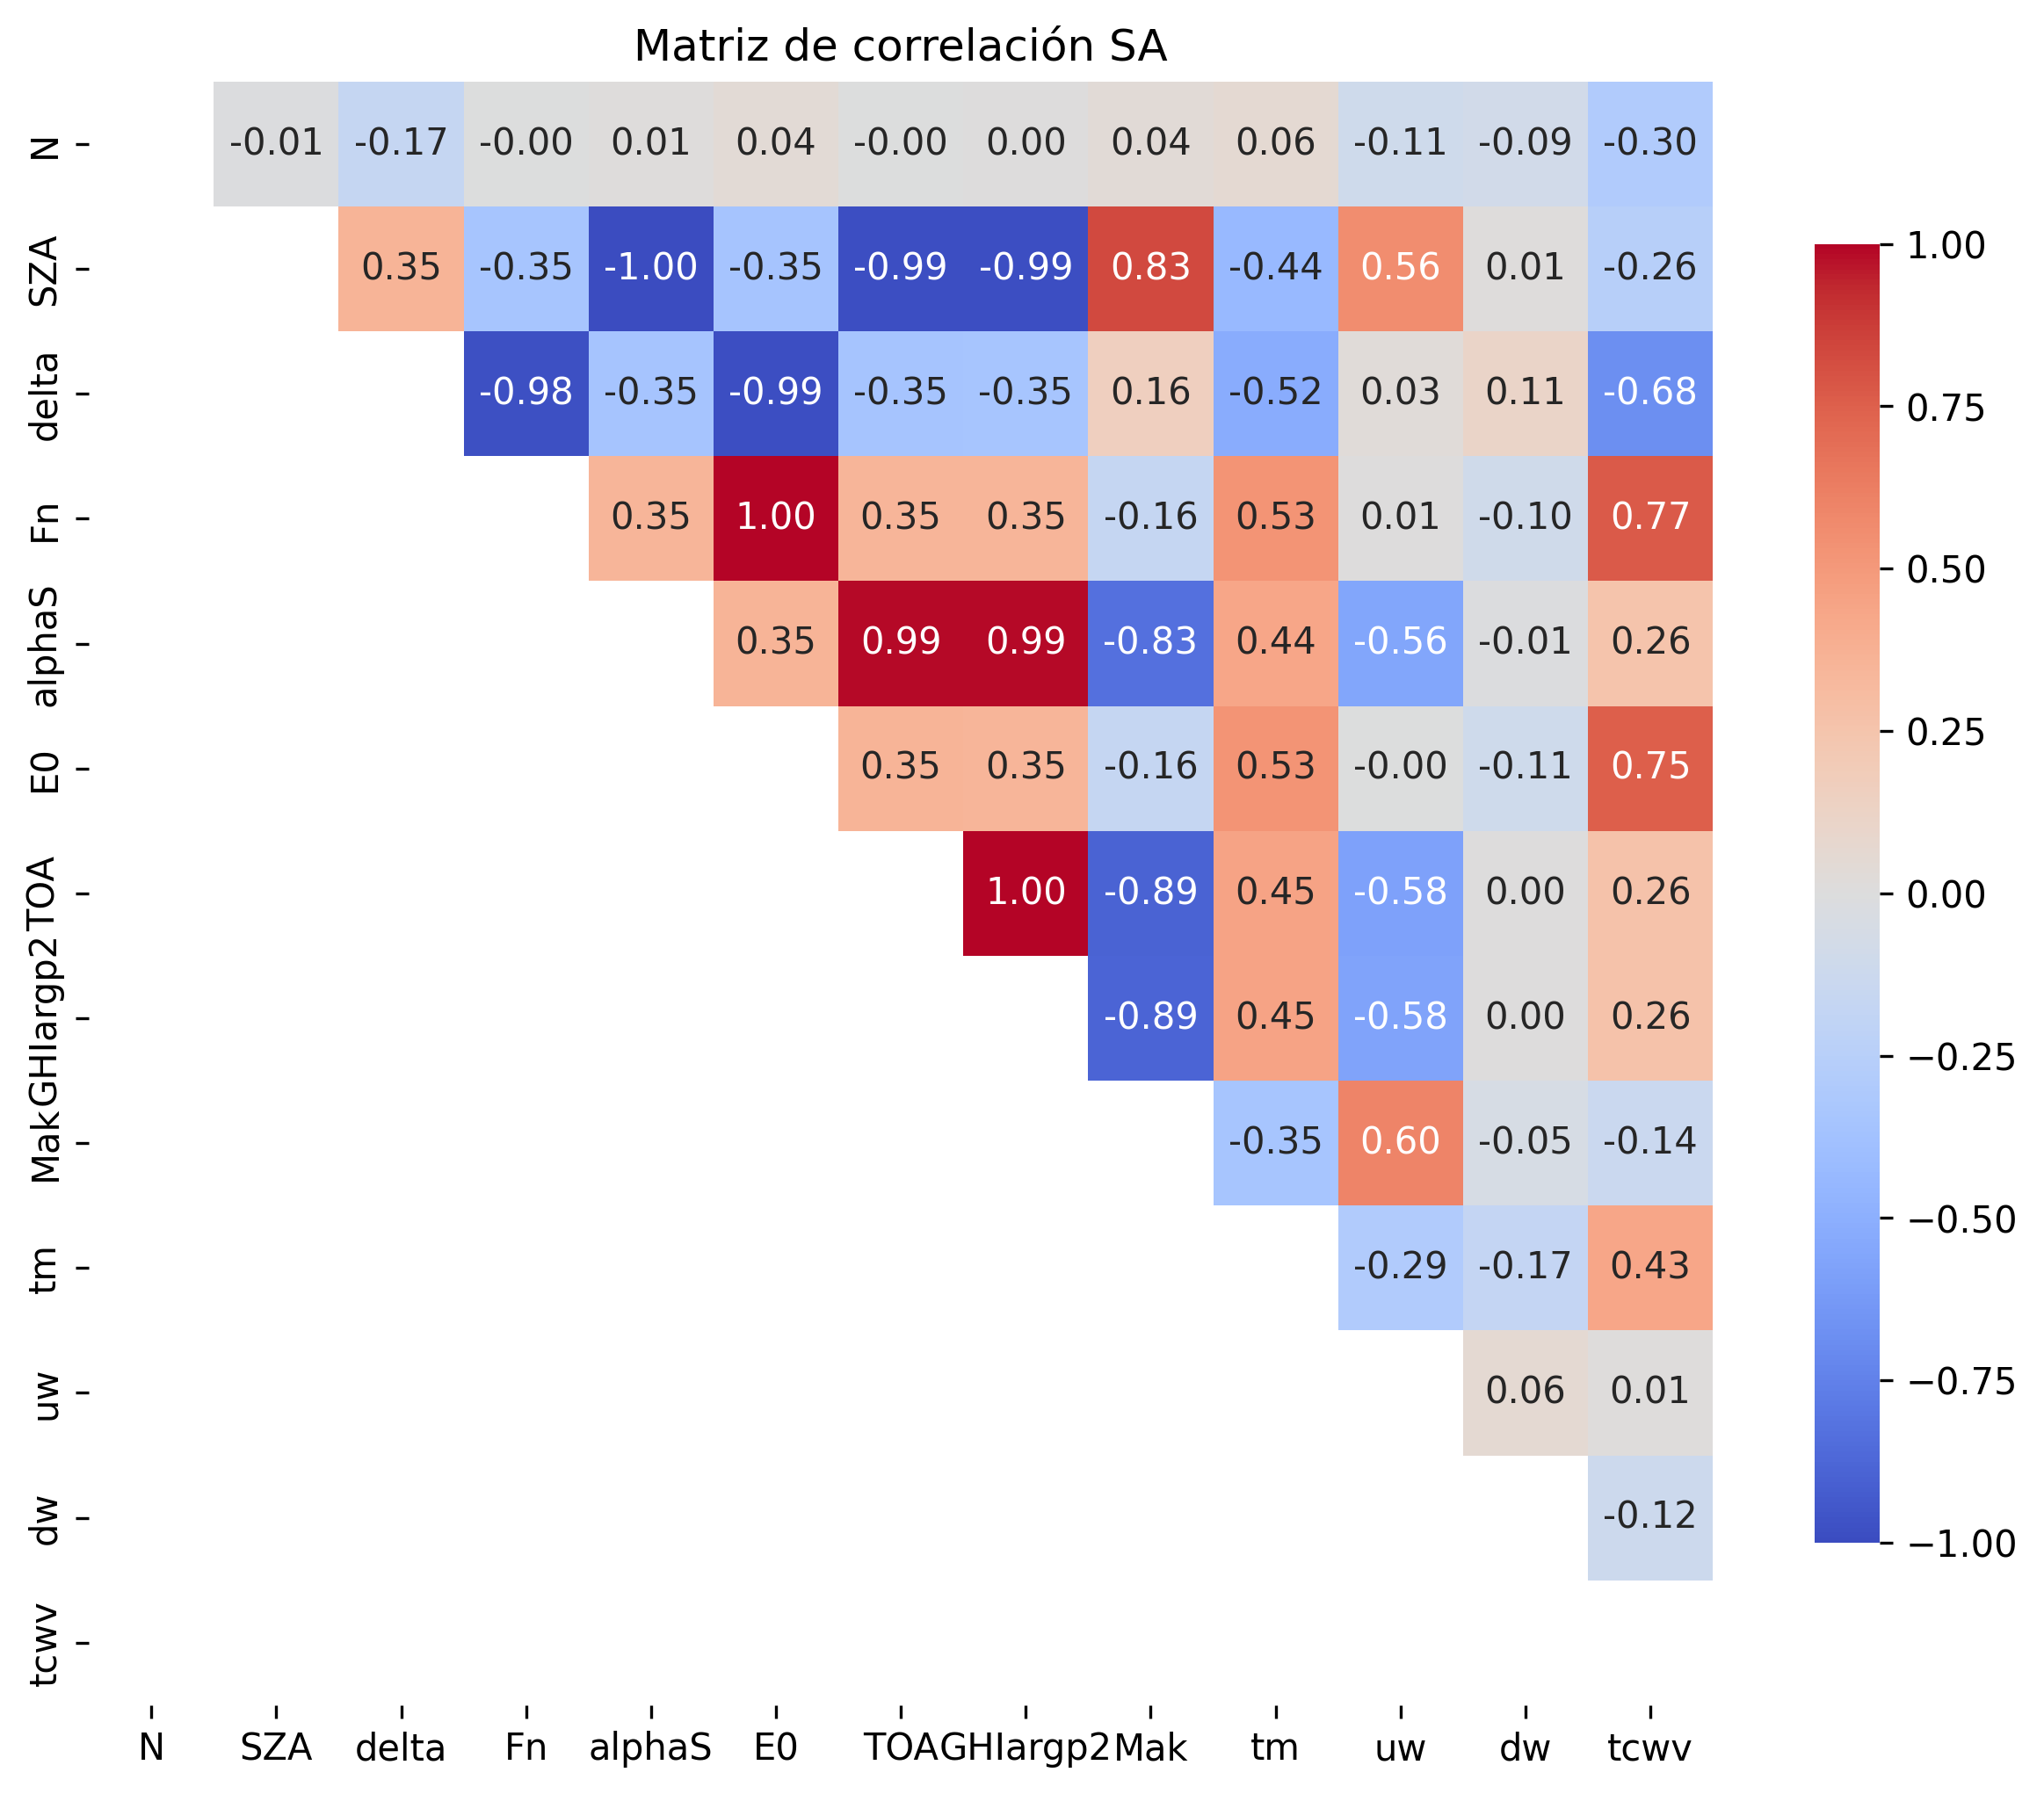
\includegraphics[width=\textwidth]{SA_corr_matrix.png} 
%DIFDELCMD <     %%%
%DIFDELCMD < \caption{%
{%DIFAUXCMD
\DIFdelFL{Matriz de correlación de los regresores en la estación SA.}}
    %DIFAUXCMD
%DIFDELCMD < \label{fig:correlacion}
%DIFDELCMD < \end{figure*}
%DIFDELCMD < 

%DIFDELCMD < %%%
\DIFdel{La Figura \ref{fig:correlacion} muestra la matriz de correlación según \textbf{Pearson} de los regresores en la estación Sa, considerando únicamente las relaciones entre las variables predictoras, sin incluir su vínculo con la variable objetivo (GHI medida).
El coeficiente de Pearson mide la correlación lineal entre dos variables continuas, asumiendo que los datos siguen una distribución aproximadamente normal y que la relación entre ellos puede representarse mediante una recta. Este coeficiente es especialmente útil cuando las variables presentan una relación proporcional directa o inversa y se desea evaluar la fuerza y dirección del vínculo lineal.}%DIFDELCMD < \\
%DIFDELCMD < 

%DIFDELCMD < %%%
\DIFdel{Este análisis es fundamental, ya que permite identificar variables que presentan una alta correlación entre sí y, por tanto, aportan información redundante. Incluir todas estas variables en el modelo puede generar problemas de multicolinealidad, dificultar la interpretación de los coeficientes y aumentar el riesgo de sobreajuste. Además, reducir la redundancia contribuye a simplificar el modelo y disminuir la carga computacional, lo cual resulta especialmente relevante en algoritmos de mayor complejidad, como MLP o modelos de tipo XGBoost. En este sentido, la matriz de correlación constituye un primer paso clave en la selección de variables, que posteriormente debe complementarse con el análisis de la relación de cada regresor con la variable objetivo, con el fin de construir modelos más eficientes, interpretables y generalizables.}%DIFDELCMD < \\
%DIFDELCMD < 

%DIFDELCMD < %%%
\DIFdel{Según \citet{Geher2016}, existen umbrales de correlación a partir de los cuales puede considerarse que dos variables están fuertemente asociadas. De acuerdo con estos autores, las correlaciones entre 0 y ±0.3 se consideran débiles, entre ±0.3 y ±0.7 moderadas, y entre ±0.7 y ±1.0 fuertes. Por tanto, en este trabajo se propone eliminar aquellas variables que podrían resultar redundantes cuando su coeficiente de correlación sea mayor a 0.85 o menor a –0.85, de modo que se reduzca la colinealidad y se mejore la estabilidad del modelo.
}%DIFDELCMD < 

%DIFDELCMD < \begin{figure*}
%DIFDELCMD <     \centering
%DIFDELCMD <     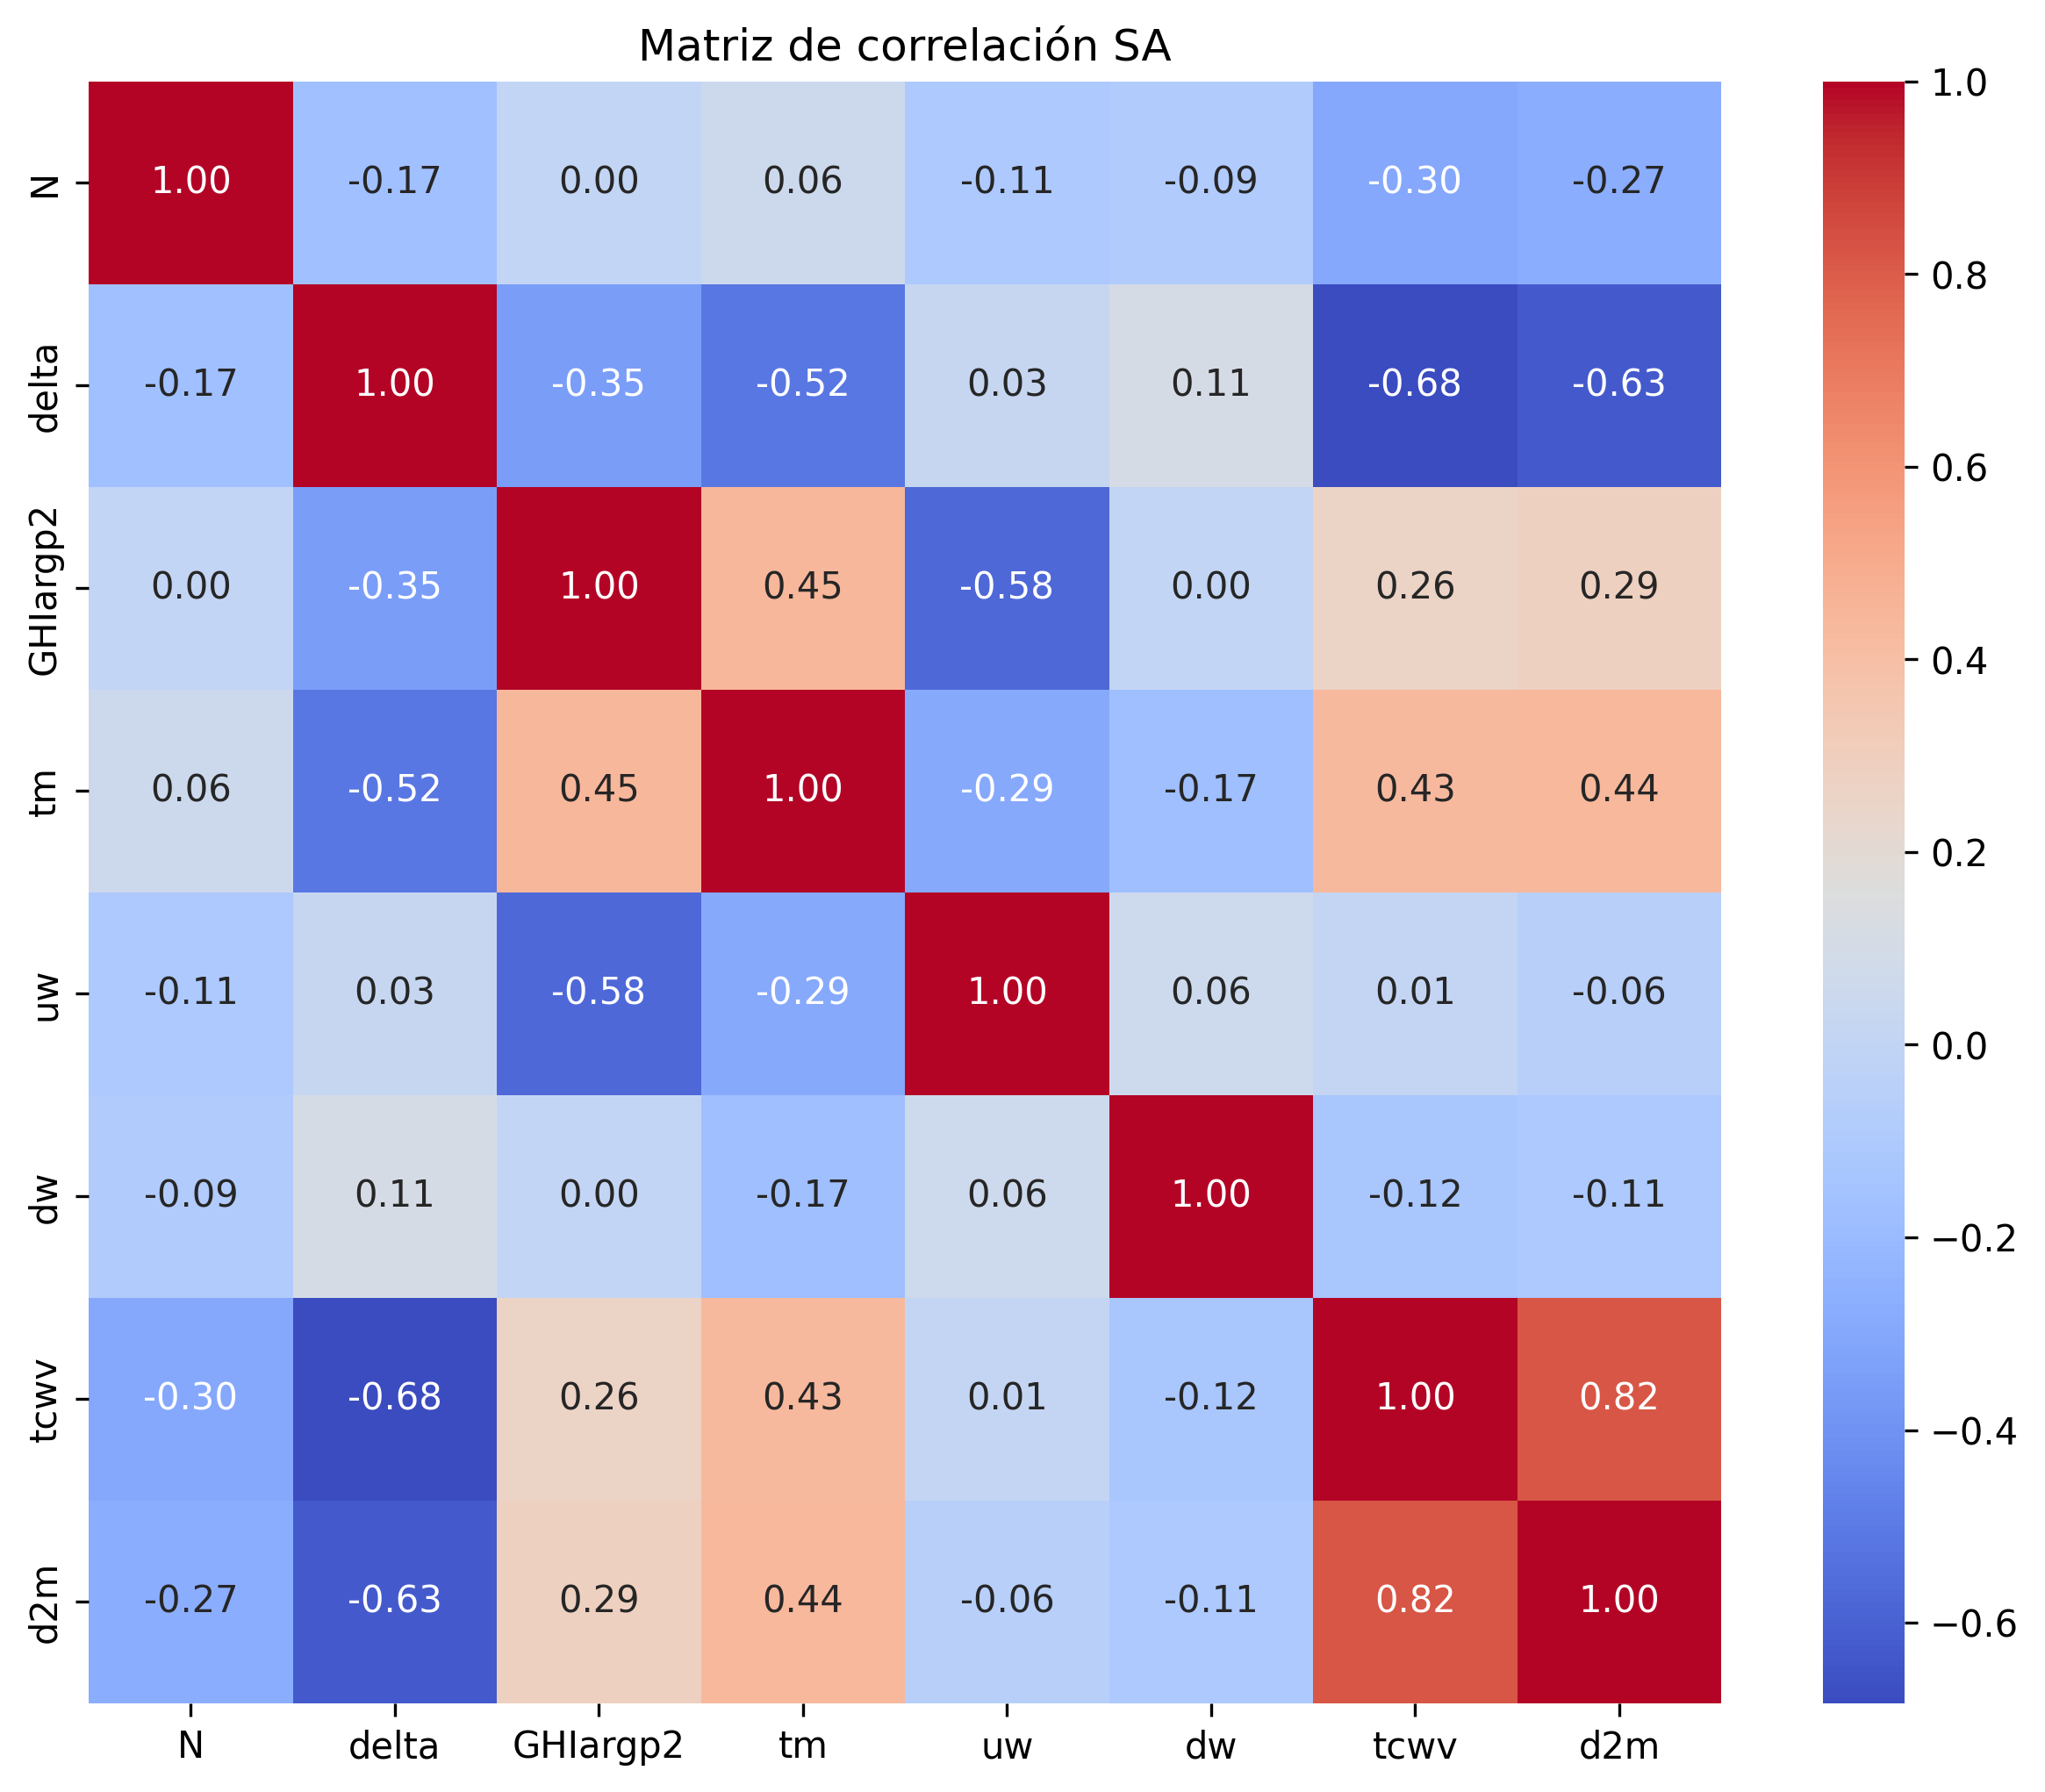
\includegraphics[width=\textwidth]{SA_corr_matrix_mini.png} 
%DIFDELCMD <     %%%
%DIFDELCMD < \caption[Coeficientes de correlación de Pearson y Spearman entre las variables meteorológicas y las distintas metodologías.]{%
{%DIFAUXCMD
\DIFdelFL{Coeficientes de correlación de Pearson y Spearman entre las variables meteorológicas y las distintas metodologías (Yu, Sa, Sca, Ero y Lq).}}
    %DIFAUXCMD
%DIFDELCMD < \label{fig:correlacion_filtrados}
%DIFDELCMD < \end{figure*}
%DIFDELCMD < 

%DIFDELCMD < %%%
\DIFdel{La Figura \ref{fig:correlacion_filtrados} presenta la matriz de correlación con el conjunto de variables regresores reducidos para la estación SA, este mismo procedimiento fue aplicado para las demás estaciones.
}%DIFDELCMD < 

%DIFDELCMD < %%%
\DIFdel{En este punto se puede analizar la relación que puede existir entre las variables regresoras y la variable objetivo. Una de las estratégias más utilizadas es la de nuevamente analizar la correlación pero ahora respecto a la medida. En la Tabla presentamos los resultados que expresa el estadístico de Pearson y \textbf{Spreman}. }%DIFDELCMD < \\
%DIFDELCMD < 

%DIFDELCMD < %%%
\DIFdel{El coeficiente de Spearman \citep{Spearman1904} es una medida no paramétrica de correlación basada en los rangos de los datos. No requiere que la relación sea lineal ni que las variables estén normalmente distribuidas. Su aplicación resulta apropiada cuando existen relaciones monótonas no lineales o cuando los datos pueden estar afectados por valores atípicos que distorsionan la correlación de Pearson.
}%DIFDELCMD < 

%DIFDELCMD < %%%
\DIFdel{El uso conjunto de ambos estadísticos permite contrastar la robustez de las asociaciones detectadas. Si ambos coeficientes son similares en magnitud y signo, se puede inferir que la relación entre las variables es consistente, tanto en términos lineales como monotónicos. En cambio, diferencias notables entre ambos valores podrían indicar la presencia de relaciones no lineales o la influencia de valores extremos.}%DIFDELCMD < \\
%DIFDELCMD < 

%DIFDELCMD < \begin{table*}[h]
%DIFDELCMD < %%%
%DIFDELCMD < \caption[Coeficientes de correlación de Pearson y Spearman entre las variables meteorológicas y las distintas metodologías.]{%
{%DIFAUXCMD
\DIFdelFL{Coeficientes de correlación de Pearson y Spearman entre las variables meteorológicas y las distintas metodologías (Yu, Sa, Sca, Ero y Lq).}}
%DIFAUXCMD
%DIFDELCMD < \label{tab:correlacion}
%DIFDELCMD < \centering
%DIFDELCMD < \resizebox{\linewidth}{!}{
%DIFDELCMD < \def\arraystretch{1.5}
%DIFDELCMD < \begin{tabular}{ccccccccccc}
%DIFDELCMD < \hline
%DIFDELCMD <  & \multicolumn{2}{c}{Yu} & \multicolumn{2}{c}{Sa} & \multicolumn{2}{c}{Sca} & \multicolumn{2}{c}{Ero} & \multicolumn{2}{c}{Lq} \\
%DIFDELCMD < \hline
%DIFDELCMD <  & Pearson & Spearman & Pearson & Spearman & Pearson & Spearman & Pearson & Spearman & Pearson & Spearman \\
%DIFDELCMD < \hline
%DIFDELCMD < GHIargp2 & 0.71 & 0.71 & 0.71 & 0.71 & 0.85 & 0.86 & 0.85 & 0.85 & 0.87 & 0.87 \\
%DIFDELCMD < N & 0.02 & 0.04 & 0.00 & 0.00 & 0.05 & 0.10 & 0.20 & 0.20 & 0.03 & 0.03 \\
%DIFDELCMD < $\delta$ & -0.24 & -0.21 & -0.12 & -0.09 & -0.13 & -0.11 & -0.22 & -0.24 & -0.11 & -0.11 \\
%DIFDELCMD < tm & 0.55 & 0.54 & 0.47 & 0.48 & 0.41 & 0.44 & 0.47 & 0.50 & 0.44 & 0.44 \\
%DIFDELCMD < uw & -0.25 & -0.26 & -0.45 & -0.46 & -0.26 & -0.28 & -0.25 & -0.30 & 0.15 & 0.16 \\
%DIFDELCMD < dw & -0.15 & -0.17 & 0.04 & 0.03 & -0.11 & -0.15 & 0.20 & 0.21 & -0.10 & -0.11 \\
%DIFDELCMD < tcwv & 0.13 & 0.12 & 0.04 & 0.02 & 0.02 & 0.03 & 0.01 & 0.05 & 0.00 & 0.00 \\
%DIFDELCMD < d2m & 0.09 & 0.08 & 0.07 & 0.06 & -0.02 & -0.01 & 0.04 & 0.05 & 0.02 & -0.01 \\
%DIFDELCMD < \hline
%DIFDELCMD < \end{tabular}}
%DIFDELCMD < \end{table*}
%DIFDELCMD < 

%DIFDELCMD < %%%
\DIFdel{Los resultados presentados en la Tabla \ref{tab:correlacion} muestran una alta consistencia entre los coeficientes de Pearson y Spearman, lo que indica que las asociaciones entre las variables meteorológicas y las metodologías evaluadas son monótonas y predominantemente lineales.
}%DIFDELCMD < 

%DIFDELCMD < %%%
\DIFdel{La variable GHIargp2 exhibe las correlaciones más elevadas con todas las metodologías, con valores entre 0.71 y 0.87, lo que evidencia una fuerte relación positiva. Este resultado sugiere que la irradiancia global tiene una influencia directa y significativa sobre los resultados obtenidos por las distintas metodologías, siendo además una de las variables de mayor peso físico en los procesos radiativos y energéticos de superficie.
}%DIFDELCMD < 

%DIFDELCMD < %%%
\DIFdel{La temperatura media (tm) presenta correlaciones moderadamente positivas (0.41–0.55), lo que indica una asociación coherente con la magnitud de las estimaciones, probablemente vinculada a la relación entre temperatura, radiación y balance energético. En contraste, la variable declinación solar ($\delta$) muestra correlaciones negativas débiles (–0.24 a –0.09), lo que podría reflejar el efecto estacional sobre la disponibilidad de radiación incidente.
}%DIFDELCMD < 

%DIFDELCMD < %%%
\DIFdel{Las componentes del viento (uw y dw) presentan en general correlaciones débiles a moderadas y negativas, particularmente en los métodos Yu, Sa y Sca. Este comportamiento podría atribuirse al efecto del viento sobre la dispersión de nubosidad o el transporte de masas de aire, factores que inciden en la transmisión de la radiación solar. Sin embargo, las correlaciones positivas observadas en el método Lq sugieren posibles diferencias metodológicas o regionales en la respuesta a la dinámica atmosférica.
}%DIFDELCMD < 

%DIFDELCMD < %%%
\DIFdel{Finalmente, las variables asociadas al contenido de humedad atmosférica (tcwv y d2m) presentan correlaciones muy bajas, lo que indica una influencia limitada de la humedad que modelan dichas variables en la GHI medida en los sitios de estudio de este trabajo.
}%DIFDELCMD < 

%DIFDELCMD < %%%
\DIFdel{En conjunto, los resultados evidencian que las variables radiativas y térmicas (GHIargp2 y tm) son las de mayor relevancia en la determinación de las estimaciones de las metodologías analizadas. La similitud entre los coeficientes de Pearson y Spearman confirma la robustez y estabilidad de las correlaciones, apoyando la validez estadística y física de las relaciones identificadas.
}%DIFDELCMD < 

%DIFDELCMD < \begin{table*}
%DIFDELCMD < %%%
%DIFDELCMD < \caption[Métricas de desempeño para cada modelo en el conjunto de prubeas utilizando como regresores la GHI modelada, la GHI en condiciones de cielo claro según y TM.]{%
{%DIFAUXCMD
\DIFdelFL{Métricas de desempeño (MBE, MAE, RMSE) para cada modelo en el conjunto de prubeas de los cinco sitios utilizando como regresores la GHI modelada, la GHI en condiciones de cielo claro según Argpv2 y TM según ERA5. Los valores están normalizados y expresados como porcentajes relativos a la media de GHI en cada sitio: 429.2~W/m$^2$ (Yu), 432.9~W/m$^2$ (Sa), 554.4~W/m$^2$ (Sca), 628.4~W/m$^2$ (Ero), y 648.7~W/m$^2$ (Lq).}}
%DIFAUXCMD
%DIFDELCMD < \label{tab:metricas_3_2}
%DIFDELCMD < \centering
%DIFDELCMD < \resizebox{\linewidth}{!}{
%DIFDELCMD < \def\arraystretch{1.5}
%DIFDELCMD < \begin{tabular}{cccccccccccccccc}
%DIFDELCMD < \hline
%DIFDELCMD <       & \multicolumn{3}{c}{Yu} & \multicolumn{3}{c}{Sa} & \multicolumn{3}{c}{Sca} & \multicolumn{3}{c}{Ero} & \multicolumn{3}{c}{Lq} \\
%DIFDELCMD < Modelo & MBE & MAE & RMSE & MBE & MAE & RMSE  & MBE & MAE & RMSE & MBE & MAE & RMSE & MBE & MAE & RMSE  \\
%DIFDELCMD < \hline
%DIFDELCMD < CAMS    MLR & -2.8 & 14.5 & 21.6 & 3.3 & 18.3  & 26.5 & 1.1 & 16.4 & 23.5 & 0.5 & 12.3 & 19.6 & 1.0 & 10.2 & 16.0 \\
%DIFDELCMD < CAMS    MLP & -2.3 & 13.2 & 20.3 & 3 & 17.1 & 25.6 & 0.7 & 16.3 & 23.3 & 0.1 & 12.5  & 19.7 & 1 & 10 & 15.7 \\
%DIFDELCMD < CAMS    XGB & -1.4 & 14.2 & 21.1 & 3.0 & 18.3 & 27.1 & 0.6 & 17.1 & 24.7 & 0.0 & 13.4 & 20.7 & 1.0 & 10.5 & 16.5 \\
%DIFDELCMD < \hline
%DIFDELCMD < 

%DIFDELCMD < LSA-SAF MLR & -5.3 & 14.3 & 20.6 & 4.1 & 20.7  & 30.1 & 2.2 & 17.3 & 24.7 & 1.1 & 11.3 & 18.9 & 0.0 & 10.8 & 17.0 \\
%DIFDELCMD < LSA-SAF MLP & -5.2 & 13.7 & 20 & 3.4 & 20.0 & 29.4 & 1.7 & 17.3 & 24.5 & 0.7 & 11.6  & 18.8 & 0.5 & 10.3 & 16.2 \\
%DIFDELCMD < LSA-SAF XGB & -4.5 & 14.5 & 20.9 & 3.8 & 21.3 & 31.0 & 0.8 & 18.5 & 25.9 & 0.5 & 12.5 & 20.0 & 0.1 & 11.1 & 17.3 \\
%DIFDELCMD < \hline
%DIFDELCMD < 

%DIFDELCMD < ERA5    MLR & -3.0 & 22.7 & 31.0 & 6.3 & 26.0  & 35.5 & -0.7 & 19.6 & 26.8 & -0.9 & 12.9 & 19.5 & 0.6 & 10.5 & 17.0 \\
%DIFDELCMD < ERA5    MLP & -1.4 & 21.8 & 30.8 & 5.5 & 25.1 & 35 & -1.7 & 20 & 27.0& -1.4& 13.1  & 19.4 & 0.8 & 10.6 & 16.9 \\
%DIFDELCMD < ERA5    XGB &  0.0 & 22.9 & 32.4 & 6.0 & 26.6 & 37.0 & -3.6 & 21.3 & 29.7 & -1.2 & 13.4 & 20.3 & 0.9 & 11.2 & 17.7 \\
%DIFDELCMD < \hline
%DIFDELCMD < 

%DIFDELCMD < MERRA-2 MLR & -10.9 & 32.0 & 40.2 & 6.4 & 31.3 & 40.8 & 2.2 & 19.7 & 27.6 & 0.8 & 11.7 & 18.8 & -0.4 & 11.7 & 18.0 \\
%DIFDELCMD < MERRA-2 MLP & -7.3 & 30.5 & 38.2 & 6 & 30.3 & 39.5 & 2.1 & 19.6 & 27.4 & 0.5 & 11.6  & 18.7 & -0.5 & 11.7 & 18 \\
%DIFDELCMD < MERRA-2 XGB & -5.3 & 31.2 & 39.5 & 6.7 & 31.2 & 41.7 & 0.1 & 21.2 & 29.7 & 0.0 & 12.7 & 20.0 & -0.6 & 12.2 & 18.6 \\
%DIFDELCMD < \hline
%DIFDELCMD < \end{tabular}}
%DIFDELCMD < \end{table*}
%DIFDELCMD < 

%DIFDELCMD < \begin{figure*}
%DIFDELCMD <     \centering
%DIFDELCMD <     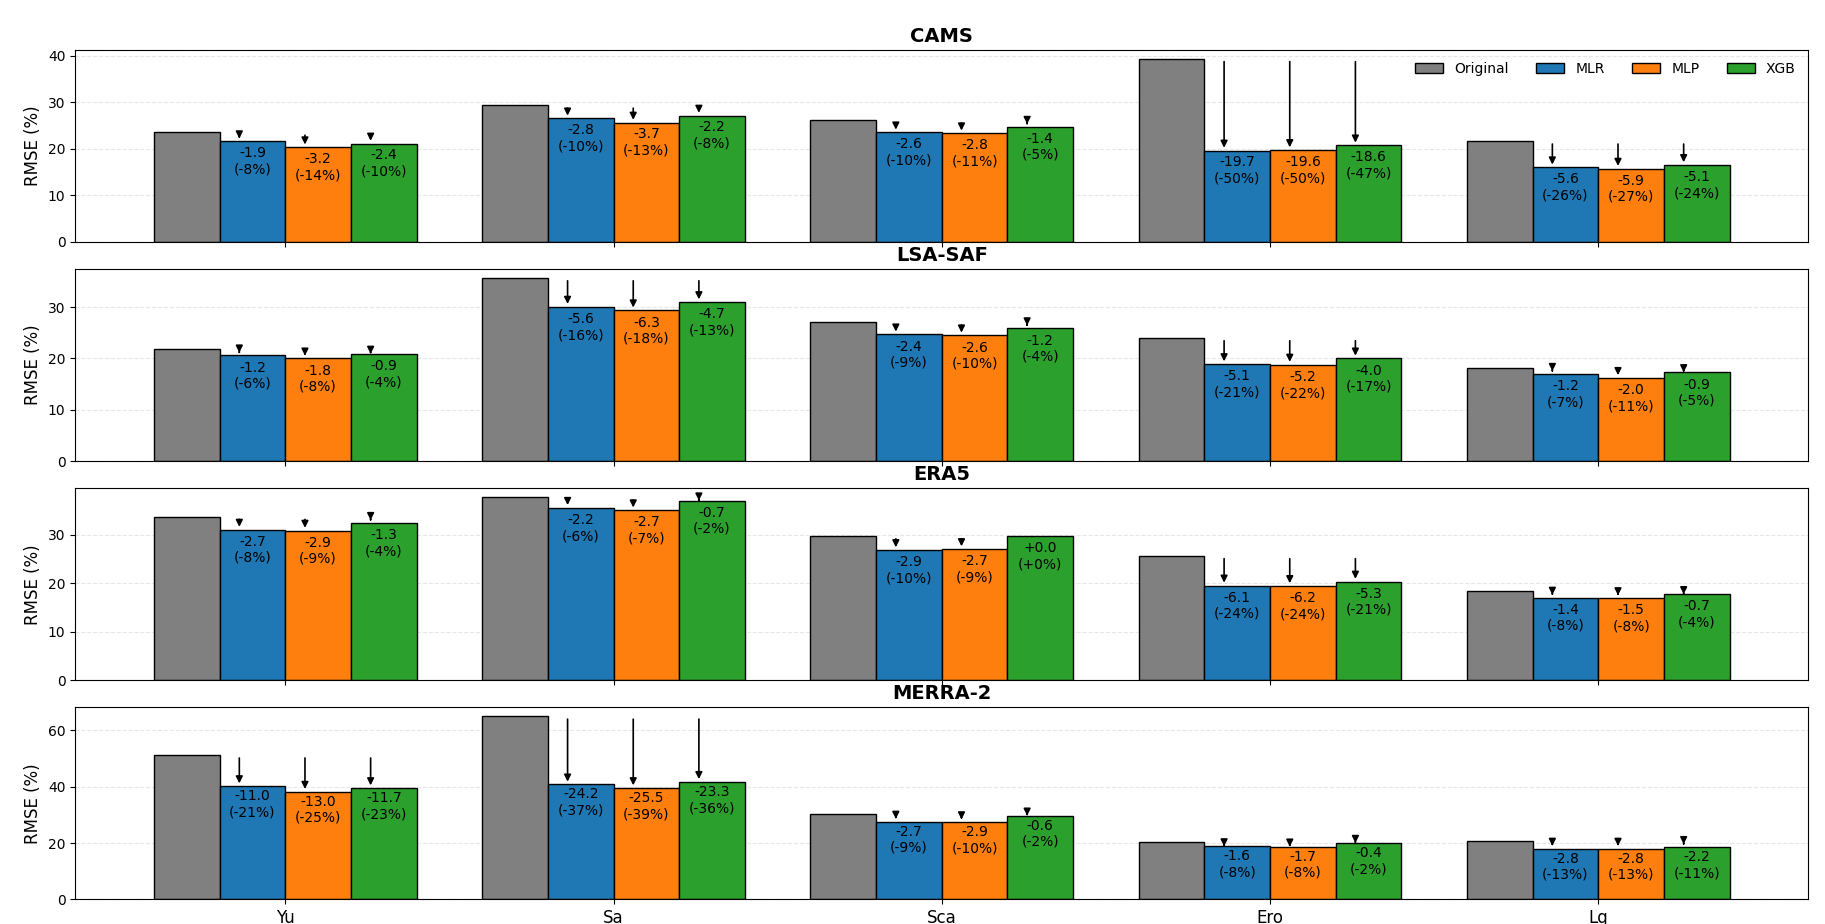
\includegraphics[width=\textwidth]{rmsd_filtrados.png} 
%DIFDELCMD <     %%%
%DIFDELCMD < \caption[Comparación del rRMSE(\%) entre estimaciones originales y las adaptaciones mediante los regresores utilizando como regresores la GHI estimada por cada modelo, GHIargp2 y tm.]{%
{%DIFAUXCMD
\DIFdelFL{Comparación del rRMSE\% entre estimaciones originales de los satélites y sus versiones adaptadas mediante los regresores MLR, MLP y XGB para los cinco sitios (Yu, Sa, Sca, Ero y Lq) utilizando como regresores la GHI estimada por cada modelo, GHIargp2 y tm. Las flechas indican mejora en la métrica adaptada respecto al valor original; las anotaciones muestran el cambio absoluto y relativo. Las flechas negras representan mejoras, mientras que las flechas rojas indican empeoramiento del desempeño respecto al modelo original.}}
    %DIFAUXCMD
%DIFDELCMD < \label{fig:comparacion_filtrados}
%DIFDELCMD < \end{figure*}
%DIFDELCMD < 

%DIFDELCMD < %%%
\DIFdel{Los resultados mostrados en la Figura \ref{fig:comparacion_filtrados} evidencian una mejora general en las métricas de desempeño cuando se restringe el conjunto de regresores a aquellas variables con influencia física y estadística demostrada sobre la irradiancia global. En particular, el uso combinado de GHIargp2 y la temperatura media (tm) permitió reducir la dispersión y aumentar la estabilidad de los modelos en todos los sitios analizados. Este comportamiento confirma que la inclusión selectiva de variables relevantes puede tener un impacto más significativo que el simple incremento del número de regresores.
}%DIFDELCMD < 

%DIFDELCMD < %%%
\DIFdel{A diferencia de los resultados previos (Tabla \ref{tab:metricas_3_1} y Figura \ref{fig:regressors_comparison}), donde algunos casos de adaptación presentaban degradaciones puntuales del desempeño (flechas rojas), en esta segunda evaluación se observa una mayor consistencia entre los sitios. Los errores relativos se mantienen dentro de márgenes similares y las diferencias entre modelos tienden a disminuir. Esta homogeneidad sugiere que una correcta selección de variables no solo mejora el ajuste local, sino que también favorece la capacidad de generalización de los modelos de regresión en distintos contextos geográficos y climáticos.
}%DIFDELCMD < 

%DIFDELCMD < %%%
\DIFdel{La reducción del conjunto de regresores elimina redundancias y disminuye la multicolinealidad, permitiendo que el modelo capture relaciones físicas más representativas. Al entrenar con un número limitado de variables influyentes, el modelo tiende a centrarse en las dependencias fundamentales entre las variables regresoras y la irradiancia medida, evitando patrones espurios que podrían inducir sobreajuste. En consecuencia, la mejora observada en las métricas no se debe necesariamente a un aumento en la capacidad del modelo, sino a una representación más fiel del fenómeno.
}%DIFDELCMD < 

%DIFDELCMD < %%%
\DIFdel{Incluir indiscriminadamente un gran número de regresores puede conducir a una falsa sensación de robustez. Aunque modelos como XGB o MLP poseen una alta capacidad para modelar relaciones no lineales, esta flexibilidad puede resultar contraproducente si las variables no aportan información relevante o presentan correlaciones espurias. De hecho, los resultados muestran que estos modelos no siempre superan sustancialmente al regresor lineal (MLR), lo que pone de manifiesto que el desempeño no depende exclusivamente de la complejidad del algoritmo, sino de la calidad y pertinencia de las variables de entrada.
}%DIFDELCMD < 

%DIFDELCMD < %%%
\DIFdel{Desde una perspectiva física, las variables radiativas (como GHIargp2) y térmicas (como la temperatura media) mantienen una relación directa con los procesos energéticos que gobiernan la radiación incidente. Por tanto, basar la selección de regresores en principios físicos conocidos ofrece una ventaja sustancial frente a estrategias puramente exhaustivas. Los modelos entrenados con variables influyentes muestran además una mayor robustez frente a condiciones cambiantes, como variaciones estacionales o diferencias en la nubosidad local. Esto sugiere que la selección adecuada de regresores no solo mejora la precisión puntual, sino que también reduce la sensibilidad del modelo a fluctuaciones de corto plazo, favoreciendo una respuesta más estable en el tiempo.
}%DIFDELCMD < 

%DIFDELCMD < %%%
\DIFdel{El uso de variables con significado físico universal facilita, además, la transferencia de modelos entre sitios. Al depender de relaciones fundamentales entre la radiación y las condiciones atmosféricas, los modelos ajustados con este tipo de regresores pueden aplicarse en regiones distintas sin necesidad de recalibraciones extensas. Este aspecto resulta especialmente relevante en contextos donde los datos locales son escasos o incompletos.
}%DIFDELCMD < 

%DIFDELCMD < %%%
\DIFdel{Los resultados refuerzan la idea de que no es apropiado seleccionar variables de manera empírica o arbitraria. El proceso de selección debe combinar análisis exploratorio, criterios físicos y métodos estadísticos (por ejemplo, correlaciones, importancia de variables o técnicas de selección embebida). Este enfoque permite identificar variables realmente informativas y descartar aquellas redundantes o poco influyentes, optimizando el equilibrio entre complejidad y rendimiento.
}%DIFDELCMD < 

%DIFDELCMD < %%%
\DIFdel{Cabe destacar que, aunque la reducción del conjunto de variables mejora el desempeño, el proceso de selección manual puede resultar subjetivo y dependiente del criterio del investigador. En este sentido, la aplicación de métodos automáticos de selección de características (como RFE, LASSO o el análisis de importancia por permutación) podría complementar el análisis físico y contribuir a establecer un marco reproducible para la construcción de modelos más eficientes. Si bien este aspecto no se abordó en el presente trabajo, consideramos que sería altamente recomendable en estudios futuros, especialmente si se amplía significativamente el conjunto de regresores.
}%DIFDELCMD < 

%DIFDELCMD < %%%
\DIFdel{En resumen, los resultados demuestran que la relevancia y coherencia física de las variables son factores determinantes para la calidad y estabilidad de los modelos de adaptación. Incluso los algoritmos más avanzados tienen un alcance limitado si se entrenan con variables poco representativas. Por ello, antes de recurrir a modelos cada vez más complejos, resulta preferible invertir esfuerzo en la búsqueda, evaluación y validación de regresores adecuados, o explorar herramientas provenientes de otras áreas —como la estadística o la visión por computadora— que contribuyan a mejorar el proceso de adaptación al sitio.
}%DIFDELCMD < 

%DIFDELCMD < %%%
\section{\DIFdel{Adaptación al sitio usando celdas satelitáles adyacentes al sitio de interés}}%DIFAUXCMD
\addtocounter{section}{-1}%DIFAUXCMD
%DIFDELCMD < \label{sec:03}
%DIFDELCMD < 

%DIFDELCMD < %%%
\DIFdel{En las Secciones \ref{sec:01} y \ref{sec:02} se presentaron las primeras evaluaciones del proceso de adaptación al sitio en la región del NOA, siguiendo metodologías previamente reportadas en la literatura relacionada. Estas implementaciones proporcionaron una base sólida para comprender la influencia del entorno local en la variable GHI y para dimensionar los límites de mejora que pueden alcanzarse al aplicar dichos enfoques.}%DIFDELCMD < \\
%DIFDELCMD < 

%DIFDELCMD < %%%
\DIFdel{Las evaluaciones realizadas, tanto en este trabajo como en estudios previos sobre SA, se han basado exclusivamente en datos medidos en una estación meteorológica que se combinan con una o más variables modeladas —provenientes de una celda de un modelo satelital o de reanálisis— que representan geográficamente la ubicación de dicha estación. En otras palabras, la información utilizada para entrenar y validar los modelos de corrección se limita a la celda específica del punto de medición, sin considerar el contexto espacial más amplio que podría aportar información adicional relevante.}%DIFDELCMD < \\
%DIFDELCMD < 

%DIFDELCMD < %%%
\DIFdel{Esta restricción impone una limitación intrínseca: la información proveniente de los productos satelitales se encuentra confinada a una única celda, definida por la resolución del modelo. En este trabajo se propone ampliar el alcance espacial de los datos de entrada incorporando valores de GHI modelados en celdas satelitales o de reanálisis adyacentes. La hipótesis central es que la variabilidad de la irradiancia solar en un punto no es un fenómeno aislado, sino que forma parte de una estructura espacialmente coherente gobernada por la dinámica atmosférica regional. Hasta el momento, no se han encontrado antecedentes que apliquen explícitamente este enfoque al proceso de adaptación al sitio.}%DIFDELCMD < \\
%DIFDELCMD < 

%DIFDELCMD < %%%
\DIFdel{Al incluir las estimaciones de irradiancia de las celdas vecinas como predictores adicionales, el modelo accede a una representación espacial más completa, lo que mejora su capacidad para identificar patrones complejos y generalizar de manera más efectiva.}%DIFDELCMD < \\
%DIFDELCMD < 

%DIFDELCMD < \noindent
%DIFDELCMD < %%%
\DIFdel{Esta idea puede entenderse mediante una analogía sencilla: cada celda satelital o de re-analásis puede imaginarse como una \emph{cámara de observación} que registra la irradiancia solar sobre una porción finita de la superficie terrestre. La estación meteorológica se encuentra dentro del campo de visión de una de esas cámaras —la celda central—, que proporciona una estimación promedio del recurso solar en dicho punto. Sin embargo, es probable que esta cámara no pueda captar completamente los fenómenos atmosféricos que se desarrollan en los bordes de su área, tales como el paso de nubes, la llegada de masas de aire o la variación en la carga de aerosoles. Suena natural que estos procesos se extiendan más allá de los límites de una celda, manifestándose parcialmente en las celdas vecinas.
}%DIFDELCMD < 

%DIFDELCMD < %%%
\DIFdel{Desde esta perspectiva, la información contenida en las celdas adyacentes actúa como una \emph{visión periférica} del entorno atmosférico que rodea al punto de interés. Al incorporar dichas celdas como variables predictoras, el modelo de adaptación al sitio accede a una representación más completa del contexto espacial. En otras palabras, utilizar únicamente la celda que contiene a la estación es equivalente a observar el cielo a través de una ventana; en cambio, incluir las celdas vecinas permite “salir al jardín” y percibir el desplazamiento de las nubes y otros patrones regionales que influyen directamente sobre la irradiancia local. Este enfoque reconoce, por tanto, que la variabilidad de la GHI en un punto no es un fenómeno aislado, sino el resultado de una dinámica espacialmente coherente gobernada por la atmósfera regional.
}%DIFDELCMD < 

%DIFDELCMD < \begin{figure}
%DIFDELCMD <     \centering
%DIFDELCMD <     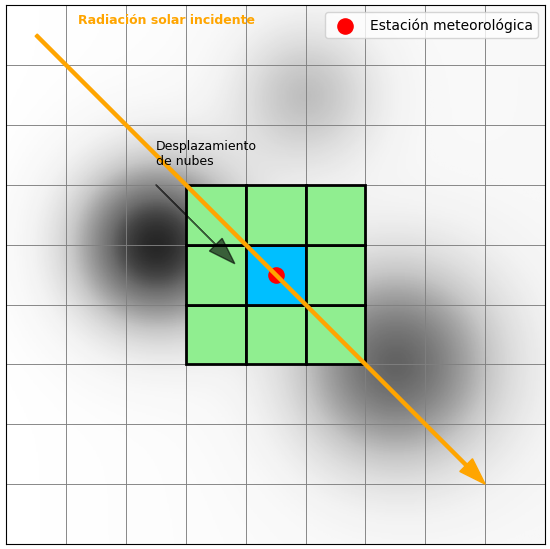
\includegraphics[width=0.5\textwidth]{figuras/AnalogiaVecinos.png}
%DIFDELCMD <     %%%
%DIFDELCMD < \caption{%
{%DIFAUXCMD
\DIFdelFL{Analogía espacial: celdas del producto de GHI y dinámica atmosférica}}
    %DIFAUXCMD
%DIFDELCMD < \label{fig:analogiaVecinos}
%DIFDELCMD < \end{figure}
%DIFDELCMD < 

%DIFDELCMD < %%%
\DIFdel{La Figura \ref{fig:analogiaVecinos} describe gráficamente la analogía desarrollada. Las tonalidades grises representan el campo de nubes o aerosoles, que se extiende entre celdas (no respeta los límites). La celda azul contiene tu estación (el punto de interés). Las celdas verdes vecinas capturan información de esa estructura atmosférica continua. El rayo solar naranja simboliza la irradiancia (GHI) afectada por esas nubes. Así se ve claramente que la información relevante para la GHI local no está confinada en la celda central, sino que fluye espacialmente.}%DIFDELCMD < \\
%DIFDELCMD < 

%DIFDELCMD < %%%
\DIFdel{Es decir que, este enfoque busca aprovechar correlaciones bien documentadas en los campos de irradiancia solar, impulsadas por el movimiento de nubes, el transporte de aerosoles y los sistemas meteorológicos a escala sinóptica \citep{IHSAN2024}. A diferencia de los métodos tradicionales de SA, que se limitan a variables locales dentro de una sola celda, el marco propuesto utiliza de manera innovadora la irradiancia satelital de las celdas circundantes como características de entrada para los modelos de aprendizaje automático. Hasta ahora, ningún trabajo había explorado explícitamente esta integración del contexto espacial.}%DIFDELCMD < \\
%DIFDELCMD < 

%DIFDELCMD < \begin{figure}
%DIFDELCMD <     \centering
%DIFDELCMD <     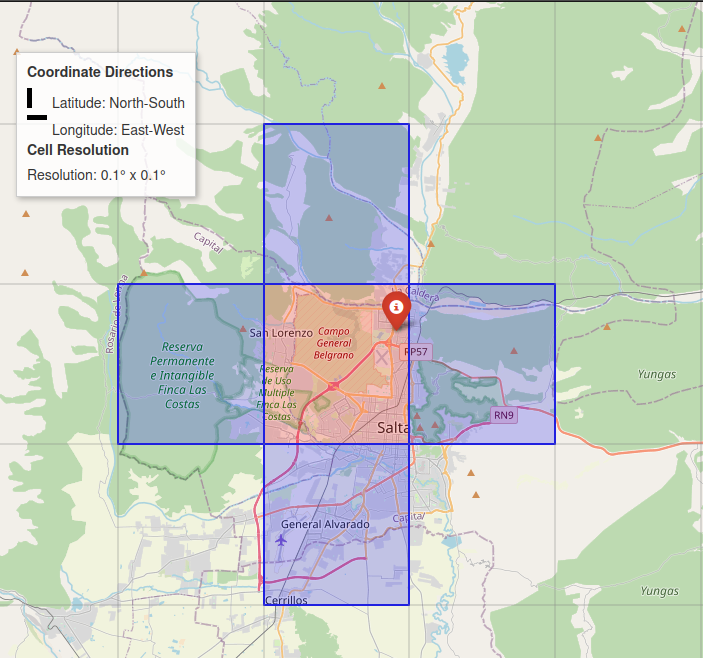
\includegraphics[width=0.7\textwidth]{figuras/gridSA.png}
%DIFDELCMD <     %%%
%DIFDELCMD < \caption{%
{%DIFAUXCMD
\DIFdelFL{Grilla utilizada por el modelo Helisat-4 de CAMS distribuido por CAMS Volume.}}
    %DIFAUXCMD
%DIFDELCMD < \label{fig:gridSA}
%DIFDELCMD < \end{figure}
%DIFDELCMD < 

%DIFDELCMD < %%%
\DIFdel{Este enfoque asume que las celdas adyacentes \ref{fig:gridSA} están sujetas a condiciones atmosféricas similares —particularmente la cobertura de nubes— que la celda central. Dada la resolución espacial de los productos satelitales (~16 km para CAMS), es razonable esperar que los valores de GHI en las celdas vecinas estén altamente correlacionados con aquellos medidos en la celda que contiene la estación en tierra. Además, considerando que, para cualquier producto de radiación de servicios como CAMS, LSA-SAF, ERA5 o MERRA-2, el GHI modelado suele ser la variable más correlacionada con el GHI observado, tiene sentido elegir este producto como base para la adaptación al sitio y la incorporación de regresores espaciales adicionales que capturen la variabilidad local.
}%DIFDELCMD < 

%DIFDELCMD < %%%
\DIFdel{La adaptación propuesta integra estos regresores distribuidos espacialmente dentro del marco de aprendizaje automático. El valor adaptado de GHI se estima como:
}%DIFDELCMD < 

%DIFDELCMD < %%%
\begin{displaymath}
\DIFdel{GHI_{adaptado} = ML_{Regresor}(GHI_{modelado}, X_{ij}),
%DIFDELCMD < \label{ec:SiteAdap}%%%
}\end{displaymath}%DIFAUXCMD
%DIFDELCMD < 

%DIFDELCMD < \noindent %%%
\DIFdel{donde $ML_{Regresor}$ denota un modelo de aprendizaje automático entrenado con el conjunto de datos, $GHI_{modelado}$ es el GHI modelado perteneciente a algùn servicio (CAMS, LSA-SAF, etc) en el sitio de interés, y $X_{ij}$ representa los valores de GHI de las celdas circundantes obtenidos del producto correspondiente.
}%DIFDELCMD < 

%DIFDELCMD < %%%
\DIFdel{La selección de celdas vecinas se basa en la distancia Manhattan (MD), definida como:
}%DIFDELCMD < 

%DIFDELCMD < %%%
\begin{displaymath}
\DIFdel{DM = \frac{|\text{lat}p - \text{lat}{ac}|}{\Delta} + \frac{|\text{lon}p - \text{lon}{ac}|}{\Delta},
%DIFDELCMD < \label{ec:dist}%%%
}\end{displaymath}%DIFAUXCMD
%DIFDELCMD < 

%DIFDELCMD < \noindent %%%
\DIFdel{donde $\Delta$ es la resolución de la grilla, $(lat_{p}, lon_{p})$ denota las coordenadas geográficas del punto de interés, y $(lat_{ac}, lon_{ac})$ corresponde a las coordenadas de una celda vecina (adyacente).
}%DIFDELCMD < 

%DIFDELCMD < %%%
\DIFdel{La MD permite identificar automáticamente las celdas satelitales adyacentes que rodean la celda central donde se encuentra la estación en tierra. Consideramos que esta métrica es adecuada porque, los productos de los servicios de estimación están organizados en una cuadrícula regular de latitud–longitud, formando una malla rectangular. En dicha grilla, las celdas se alinean en filas y columnas, y la MD, definida como la suma de las diferencias absolutas en latitud y longitud normalizadas por la resolución de la grilla, captura efectivamente el número de pasos necesarios para alcanzar una celda vecina tanto horizontal como verticalmente.}%DIFDELCMD < \\
%DIFDELCMD < 

%DIFDELCMD < %%%
\DIFdel{Las celdas con $DM=1$ son directamente adyacentes a la celda central (es decir, al norte, sur, este u oeste), siendo las más relevantes para capturar la variabilidad espacial local de las condiciones atmosféricas. A diferencia de la distancia euclidiana, que enfatiza la proximidad radial, la MD refleja mejor las relaciones de vecindad en productos satelitales en grilla, asegurando que la información espacial utilizada para la adaptación site-specific sea consistente con la estructura regular del producto.}%DIFDELCMD < \\
%DIFDELCMD < 

%DIFDELCMD < %%%
\DIFdel{En conjunto, esta metodología permite que la adaptación del GHI al sitio integre tanto la estimación directa del producto satelital como la información de celdas vecinas, mejorando la capacidad de predicción local y la transferencia del modelo a diferentes condiciones espaciales.}%DIFDELCMD < \\
%DIFDELCMD < 

%DIFDELCMD < \begin{table*}%%%
%DIF < []
  %DIFDELCMD < \centering
%DIFDELCMD <   

%DIFDELCMD <   %%%
%DIFDELCMD < \caption[Métricas de desempeño para cada modelo adaptado en el conjunto de pruebas.]{%
{%DIFAUXCMD
\DIFdelFL{Métricas de desempeño (MBE, MAE, RMSE) para cada modelo adaptado en los cinco sitios en el \textbf{conjunto de pruebas}.}}
  %DIFAUXCMD
%DIFDELCMD < \label{tab:metrics-as-4}
%DIFDELCMD <   \resizebox{\linewidth}{!}{%
%DIFDELCMD <     \begin{tabular}{|l|ccc|ccc|ccc|ccc|ccc|}
%DIFDELCMD <       \hline
%DIFDELCMD <       & \multicolumn{3}{c|}{YU} & \multicolumn{3}{c|}{SA} & \multicolumn{3}{c|}{SCA} & \multicolumn{3}{c|}{ERO} & \multicolumn{3}{c|}{LQ} \\
%DIFDELCMD <       \cline{2-16}
%DIFDELCMD <       Modelo  & MBE & MAE & RMSE & MBE & MAE & RMSE & MBE & MAE & RMSE & MBE & MAE & RMSE & MBE & MAE & RMSE \\
%DIFDELCMD <       \hline
%DIFDELCMD <       \multicolumn{16}{|c|}{\textit{Resolución Temporal: 15 minutos}} \\
%DIFDELCMD <       \hline
%DIFDELCMD <       LSA-SAF & 7.6  & 16.5 & 25.5 & 17.9 & 27.4 & 39.4 & 13.1 & 22.2 & 30.9 & -7.7  & 16.2 & 26.5 & 4.0  & 12.6 & 22.6 \\
%DIFDELCMD <       LSA-SAF MLR  & -5   & 16.5 & 24.6 & 3.2 & 23.8 & 35.2 & -2.9 & 18.5 & 25.7 & 1.4 & 12.8 & 21.4 & 2.8 & 12.7  & 21.7\\ 
%DIFDELCMD <       LSA-SAF MLP  & -6   & 16.4 & 24.3 & 1.9 & 23.2 & 35.3 & 1.3  & 16.7 & 25.3 & 2   & 12.5 & 21.4  & 4.7 & 12.6 & 21.7\\       
%DIFDELCMD <       LSA-SAF XGB  & -5.2 & 16.2 & 24.1 & 2.7 & 23.1 & 34.9 & -1  & 18.2 & 26.7 & 1   & 12.3 & 21.3  & 2.3 & 12.9 & 21.9\\       
%DIFDELCMD <       \hline
%DIFDELCMD <       \multicolumn{16}{|c|}{\textit{Resolución Temporal: horaria}} \\
%DIFDELCMD <       

%DIFDELCMD <       \hline
%DIFDELCMD <       

%DIFDELCMD <       LSA-SAF        & 7.5  & 14.4 & 21.8 & 17.9 & 25.3 & 35.7 & 13.3 & 20.3 & 27.1 & -7.7  & 14.8 & 24.0 & 4.8  & 10.9 & 18.2 \\
%DIFDELCMD <       LSA-SAF MLR    & -4.9 & 14.1 & 20.8 & 2.6 & 21.5 & 31.9 & -3.8 & 16.6 & 22.4 & 1.9 & 11.3 & 18.8 & 0.2 & 10.4 & 16.8\\ 
%DIFDELCMD <       LSA-SAF MLP    & 6.8  & 14.9 & 20.8 & 1.4 & 20.5 & 31   & -2.5 & 16.6 & 22.3 & 1.5 & 11.1 & 18.6 & 1.7 & 10.4 & 16.5\\ 
%DIFDELCMD < 	  LSA-SAF XGB    & 4.7  & 14.5 & 20.3 & 3.1 & 20.6 & 30.3 & -2.2 & 16   & 21.8 & 1.6 & 11.3 & 18.8 & 0.4 & 10.4 & 16.4\\
%DIFDELCMD < 	  \hline
%DIFDELCMD < 	  ERA5          & 1.2  & 22.2 & 33.7 & 9.4 & 27.1 & 37.7 & 1.9  & 20.2 & 29.7 & -14 & 19.3 & 25.6 & -0.8 & 11.3 & 18.4 \\
%DIFDELCMD <       ERA5 MLR      & 0.6  & 22.6 & 31.8 & 7   & 26.5 & 36.8 & -2.2 & 19.5 & 26.2 & 1.1 & 10.7 & 17.8 & 0.9  & 10.4 & 16.7 \\
%DIFDELCMD <       ERA5 MLP      & 1.7  & 22.7 & 33.5 & 8.3 & 26.4 & 37.2 & -2.5 & 19.8 & 26.6 & 1.4 & 10.9 & 17.9 & 1.4  & 10.4 & 16.7  \\
%DIFDELCMD < 	  ERA5 GXB      & 1.5  & 23.3 & 33.5 & 6.6 & 26.8 & 37   & -2.5 & 19.4 & 26.4 & 0.8 & 11.1 & 18.1 & 0.9  & 10.5 & 16.7\\
%DIFDELCMD <       \hline	
%DIFDELCMD < 	  MERRA-2       & 24.9 & 33.5 & 51.2 & 43.4 & 48.3 & 65.0 & 10.9 & 21.7 & 30.3 & -3.8  & 13.1 & 20.4 & 1.4  & 13.4 & 20.8 \\
%DIFDELCMD <       MERRA-2 MLR   & -2.8 & 34.4 & 43.4 & 8.2 & 32.3 & 43.2 & 1   & 20.8 & 29.1 & 0.4 & 11.5 & 18.7 & -0.4 & 11.5 & 17.9\\
%DIFDELCMD <       MERRA-2 MLP   & -4.9 & 34.5 & 43   & 9.2 & 31.6 & 43   & 1.8 & 20.7 & 29.5 & 0.2 & 11.6 & 18.7 &  0.3 & 11.4 & 17.9\\
%DIFDELCMD < 	  MERRA-2 GXB   & -4.2 & 34.2 & 43.1 & 7.9 & 32.6 & 43.2 & 0.4  & 21   & 29.7   & 0.5   & 11.6    & 18.8    & -0.3 & 11.8 & 18.2 \\
%DIFDELCMD <       \hline	
%DIFDELCMD <     \end{tabular}%
%DIFDELCMD <   }
%DIFDELCMD < \end{table*}
%DIFDELCMD < 

%DIFDELCMD < %%%
\DIFdel{En la Tabla \ref{tab:metrics-as-4} se presentan los resultados obtenidos utilizando el enfoque de adaptación propuesto. Para facilitar la comparación, también se incluyen las métricas de desempeño de los modelos sin adaptación.
}%DIFDELCMD < 

%DIFDELCMD < %%%
\DIFdel{Puede observarse que, en términos del RMSE (\%), cada modelo de estimación muestra una mejora en todos los sitios, independientemente del algoritmo de regresión empleado. Además, se observa un comportamiento similar entre los modelos basados en MLR, MLP y XGB, lo cual refuerza la conclusión previamente señalada: el aumento en la complejidad del modelo de regresión no necesariamente conduce a una mejora significativa en las métricas de desempeño.
}%DIFDELCMD < 

%DIFDELCMD < %%%
\DIFdel{Por otra parte, a partir de lo analizado en la Sección \ref{sec:02}, puede justificarse la elección de la temperatura como variable regresora adicional para mejorar el desempeño de los modelos.
}%DIFDELCMD < 

%DIFDELCMD < %%%
\DIFdel{Considerando esto, se evaluó un enfoque que combina la información proveniente de las celdas vecinas adyacentes a la celda de interés con la temperatura modelada (TM2) obtenida de ERA5. Además, dado que el modelo MLR ha mostrado un desempeño consistente y comparable al de los modelos MLP y XGB, se optó por evaluar su rendimiento en esta nueva configuración.
}%DIFDELCMD < 

%DIFDELCMD < %%%
\DIFdel{Los resultados correspondientes se presentan en la Tabla \ref{tab:metrics-final}, donde puede observarse una mejora general en las métricas, lo que evidencia el beneficio de incorporar información térmica como variable auxiliar en el proceso de adaptación.
}%DIFDELCMD < 

%DIFDELCMD < \begin{table*}%%%
%DIF < []
  %DIFDELCMD < \centering
%DIFDELCMD <   

%DIFDELCMD <   %%%
%DIFDELCMD < \caption[Métricas de desempeño del modelo ERA5 adapado en los cinco sitios en el conjunto de pruebas.]{%
{%DIFAUXCMD
\DIFdelFL{Métricas de desempeño (MBE, MAE, RMSE) del modelo ERA5 adapado en los cinco sitios en el \textbf{conjunto de pruebas}.}}
  %DIFAUXCMD
%DIFDELCMD < \label{tab:metrics-final}
%DIFDELCMD <   \resizebox{\linewidth}{!}{%
%DIFDELCMD <     \begin{tabular}{|l|ccc|ccc|ccc|ccc|ccc|}
%DIFDELCMD <       \hline
%DIFDELCMD <       & \multicolumn{3}{c|}{YU} & \multicolumn{3}{c|}{SA} & \multicolumn{3}{c|}{SCA} & \multicolumn{3}{c|}{ERO} & \multicolumn{3}{c|}{LQ} \\
%DIFDELCMD <       \cline{2-16}
%DIFDELCMD <       Modelo  & MBE & MAE & RMSE & MBE & MAE & RMSE & MBE & MAE & RMSE & MBE & MAE & RMSE & MBE & MAE & RMSE \\
%DIFDELCMD <       \hline
%DIFDELCMD <       \multicolumn{16}{|c|}{\textit{Resolución Temporal: horaria}} \\
%DIFDELCMD <       \hline
%DIFDELCMD <  

%DIFDELCMD < 	  ERA5          & 1.2   & 22.2 & 33.7 & 9.4 & 27.1 & 37.7 & 1.9  & 20.2 & 29.7 & -14 & 19.3 & 25.6 & -0.8 & 11.3 & 18.4 \\
%DIFDELCMD <       ERA5 MLR      & -0.7  & 21.9 & 30.4 & 6.7 & 26.4 & 36.2 & -2.8 & 19.5 & 25.7 & 0.6 & 10.8 & 17.6 &  0.8 & 10.2 & 16.2\\
%DIFDELCMD <       \hline
%DIFDELCMD <       \end{tabular}%
%DIFDELCMD <       }
%DIFDELCMD < \end{table*}
%DIFDELCMD < 

%DIFDELCMD < %%%
\DIFdel{Este enfoque parece consolidarse como una estrategia efectiva para mejorar la precisión de los modelos de SA aplicados a la estimación de la GHI en superficie. Los resultados obtenidos evidencian que la incorporación de información proveniente de celdas satelitales adyacentes permite capturar de forma más realista la estructura espacial de la atmósfera, lo que se traduce en reducciones consistentes del error cuadrático medio (RMSE) y, en menor medida, del error medio absoluto (MAE) en todos los sitios analizados.
}%DIFDELCMD < 

%DIFDELCMD < %%%
\DIFdel{En particular, se observa que la mejora relativa es más pronunciada en estaciones ubicadas en entornos con alta variabilidad topográfica o atmosférica, donde las discontinuidades locales en la nubosidad o la resolución espacial de los modelos aparentan introducir sesgos significativos sobre las estimaciones. En estos casos, la información espacial adicional actúa como un mecanismo de compensación que suaviza los efectos de dichas heterogeneidades.
}%DIFDELCMD < 

%DIFDELCMD < %%%
\DIFdel{Asimismo, la estabilidad del modelo MLR frente a los enfoques basados en aprendizaje profundo (MLP) o en ensamblado de árboles (XGB) refuerza la hipótesis de que la ganancia principal proviene de la incorporación de contexto espacial, más que del aumento de complejidad del algoritmo. Este hallazgo tiene implicancias prácticas relevantes: demuestra que, con un modelo lineal relativamente simple, es posible capturar buena parte de la variabilidad espacial si la información de entrada está adecuadamente estructurada.
}%DIFDELCMD < 

%DIFDELCMD < %%%
\DIFdel{Desde un punto de vista físico, la coherencia espacial del campo de irradiancia responde a procesos atmosféricos de mesoescala, como el desplazamiento de sistemas nubosos, los cuales presentan una estructura continua sobre varias decenas de kilómetros. Esta correlación natural explica por qué la estrategia de vecindad produce mejoras sistemáticas en todos los casos.
}%DIFDELCMD < 

%DIFDELCMD < %%%
\DIFdel{En los resultados presentados, las reducciones promedio en RMSE alcanzan valores del orden del 5 al 15\%, dependiendo del sitio y del producto satelital empleado. Si bien estas magnitudes pueden considerarse moderadas, adquieren gran relevancia en aplicaciones que requieren alta precisión radiativa, tales como la calibración de sistemas fotovoltaicos, la validación de modelos climáticos regionales o la planificación de infraestructura energética distribuida.
}%DIFDELCMD < 

%DIFDELCMD < %%%
\DIFdel{Otro aspecto destacable es la consistencia del comportamiento entre diferentes resoluciones temporales (15 min y horaria). Esto sugiere que la mejora introducida por el uso de celdas adyacentes no se limita a un determinado rango temporal, sino que actúa de manera robusta a distintas escalas. En consecuencia, el método podría adaptarse fácilmente a bases de datos con diferentes resoluciones o a esquemas de reanálisis con pasos de tiempo variables.
}%DIFDELCMD < 

%DIFDELCMD < \begin{figure}
%DIFDELCMD <     \centering
%DIFDELCMD <     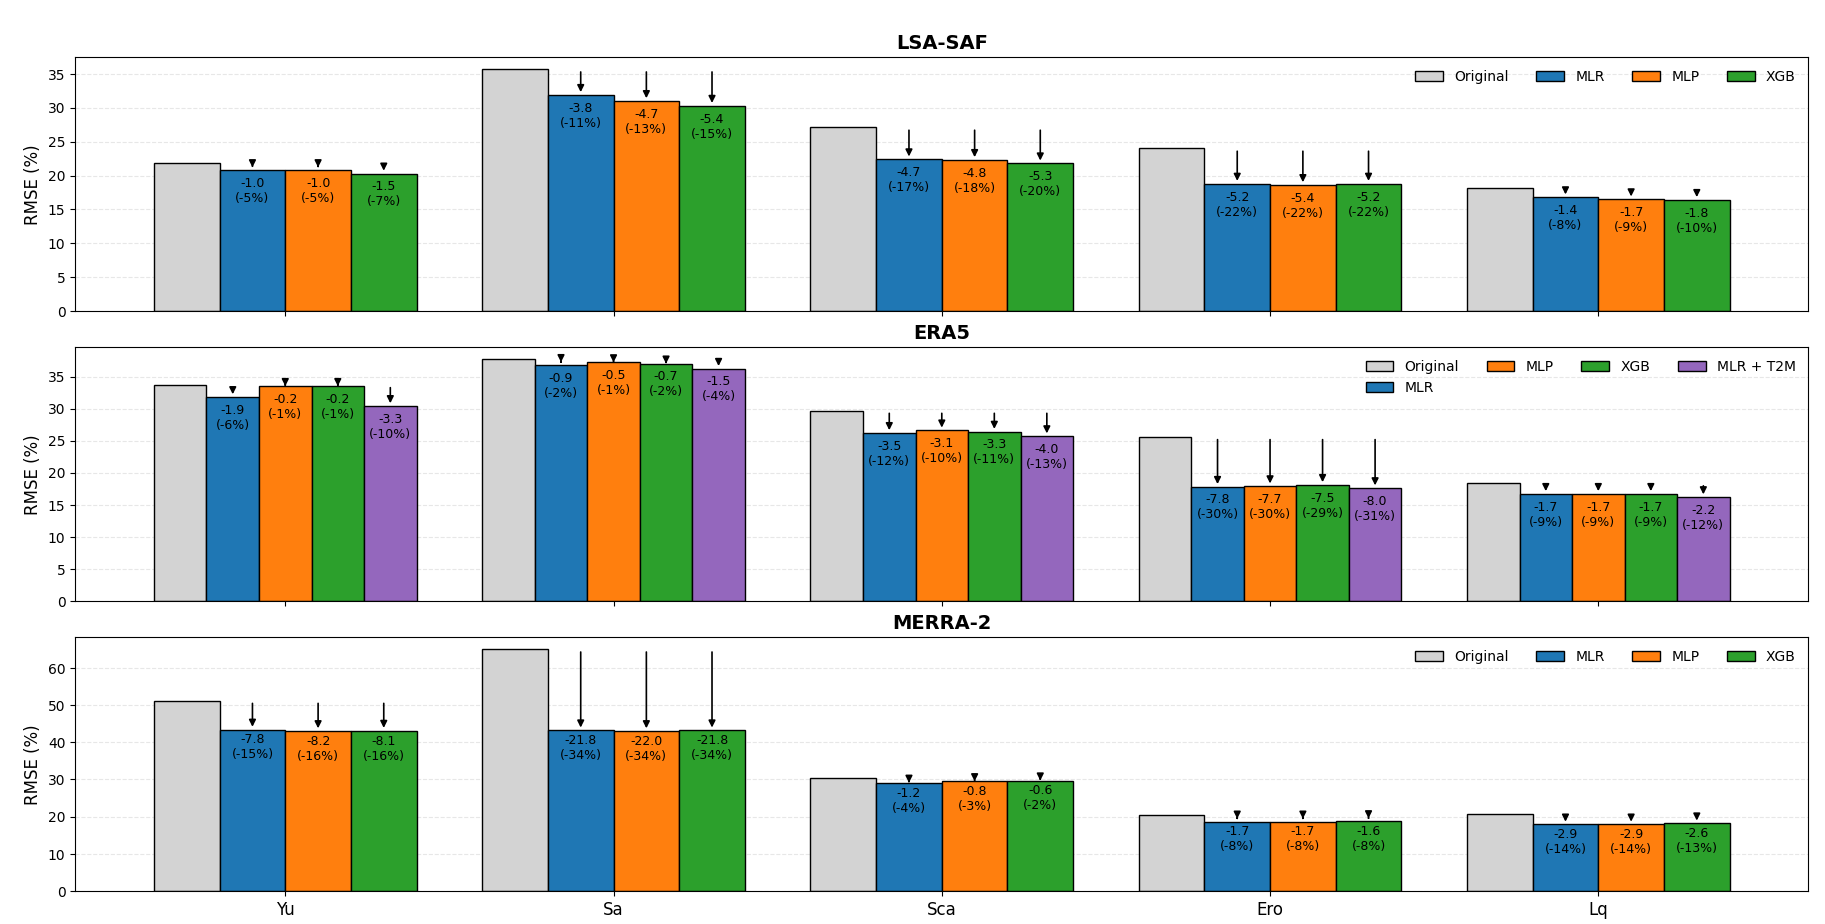
\includegraphics[width=1\textwidth]{figuras/rmsd_vecinos.png}
%DIFDELCMD <     %%%
%DIFDELCMD < \caption{%
{%DIFAUXCMD
\DIFdelFL{rRMSE(\%) comparativo para las evaluaciones utilizando el enfoque de celdas adyacentes.}}
    %DIFAUXCMD
%DIFDELCMD < \label{fig:rrmsdVecinos}
%DIFDELCMD < \end{figure}
%DIFDELCMD < 

%DIFDELCMD < %%%
\DIFdel{La incorporación adicional de la temperatura como variable auxiliar (caso TM2) refuerza la capacidad predictiva del modelo (Ver Figura \ref{fig:rrmsdVecinos}). Dado que la temperatura del aire está estrechamente ligada a los procesos de transferencia radiativa y a la presencia de nubosidad, su inclusión permite capturar efectos de segundo orden que no están completamente representados por el GHI modelado. La mejora observada en las métricas al combinar temperatura e información espacial confirma la complementariedad entre ambas fuentes de variabilidad.
}%DIFDELCMD < 

%DIFDELCMD < %%%
\DIFdel{En conjunto, los resultados respaldan la hipótesis de trabajo: la irradiancia solar medida en un sitio forma parte de un sistema espacialmente coherente, y la representación de ese sistema mediante un vecindario de celdas mejora la estimación puntual del recurso solar. De este modo, el enfoque propuesto constituye un avance metodológico que amplía el paradigma clásico de adaptación al sitio, tradicionalmente confinado a una única celda.
}%DIFDELCMD < 

%DIFDELCMD < %%%
\DIFdel{Finalmente, cabe destacar que el marco planteado mantiene un equilibrio adecuado entre complejidad y generalización. Su implementación es sencilla, no requiere aumentar de manera significativa los costos computacionales y puede integrarse en flujos de procesamiento ya existentes para la calibración de productos satelitales o de reanálisis. En este sentido, representa una alternativa práctica y científicamente fundamentada para mejorar la representatividad espacial de los modelos de irradiancia.
}%DIFDELCMD < 

%DIFDELCMD < %%%
\section{\DIFdel{Adaptación al sitio tomando consideraciones de una serie temporal}}%DIFAUXCMD
\addtocounter{section}{-1}%DIFAUXCMD
%DIFDELCMD < \label{sec:04}
%DIFDELCMD < 

%DIFDELCMD < %%%
\DIFdel{El análisis presentado en las Secciones \ref{sec:01} y \ref{sec:02} permitió establecer que, en el contexto de la adaptación al sitio (SA por sus siglas en ingles), el grado de mejora obtenido en las estimaciones de la irradiancia global horizontal (GHI) no depende necesariamente de la complejidad de los modelos regresores utilizados. Más bien, los resultados evidencian la importancia de una adecuada selección de variables regresoras para garantizar un desempeño correcto y estable de los modelos de regresión.
}%DIFDELCMD < 

%DIFDELCMD < %%%
\DIFdel{En la Sección \ref{sec:03} se exploró un enfoque que deriva los regresores a partir de la información espacial circundante en celdas adyacentes al sitio de interés. Además, estos regresores, en combinación con aquellos que mantienen una relación física directa con la GHI —como la GHI en condiciones de cielo claro y la temperatura—, condujeron a los mejores resultados obtenidos en este trabajo.
}%DIFDELCMD < 

%DIFDELCMD < %%%
\DIFdel{Por otra parte, es importante reconocer que, incluso cuando se dispone de un conjunto óptimo de variables, persisten fuentes de variabilidad que limitan la capacidad de los modelos para capturar plenamente la dinámica de la radiación solar a escala local y temporal. Una de las principales limitaciones radica en la naturaleza \textbf{no estacionaria} de la serie de irradiancia, la cual está fuertemente modulada por factores astronómicos y estacionales.
}%DIFDELCMD < 

%DIFDELCMD < %%%
\DIFdel{Este tipo de comportamiento ha sido ampliamente documentado en la literatura económica. \citet{Granger1974} demostraron que las regresiones sobre series no estacionarias pueden inducir relaciones espurias, en las que el coeficiente de determinación ($R^2$) resulta artificialmente alto sin que exista una relación causal real entre las variables. Este fenómeno, conocido como \emph{spurious regression}, se presenta cuando se aplican métodos de mínimos cuadrados a series con tendencias o raíces unitarias, lo que genera inferencias engañosas \citep{Ventosa2009}.
}%DIFDELCMD < 

%DIFDELCMD < %%%
\DIFdel{En consecuencia, la correcta identificación y tratamiento de la no estacionariedad constituye un paso fundamental para evitar correlaciones espurias y mejorar la validez de los modelos aplicados a series temporales meteorológicas. Esta limitación es general al proceso de regresión que se realiza sobre otras series temporales de diversas áreas, y resalta la necesidad de incorporar técnicas que mitiguen los efectos de la tendencia o la estacionalidad, favoreciendo la obtención de residuos estacionarios y estadísticamente consistentes.
}%DIFDELCMD < 

%DIFDELCMD < %%%
\DIFdel{En este contexto, la incorporación de técnicas que consideren explícitamente la \textbf{estructura temporal} de los datos representa un paso necesario para mejorar la capacidad de generalización de los modelos de adaptación. La \textbf{desestacionalización} de series temporales permite eliminar la componente periódica asociada a la posición solar y a los ciclos estacionales, resaltando las fluctuaciones residuales que responden a la variabilidad atmosférica real. Este procedimiento no solo facilita una representación más homogénea de los datos, sino que también posibilita que los algoritmos de aprendizaje se centren en los procesos de corto plazo, como la dinámica de nubosidad o la variación de aerosoles, factores determinantes en la modulación instantánea de la irradiancia global.
}%DIFDELCMD < 

%DIFDELCMD < %%%
\DIFdel{De manera complementaria, estudios recientes han destacado la importancia de abordar la \textbf{no linealidad} y la \textbf{no estacionariedad} de las series ambientales mediante enfoques multiescala. \citep{Schulte2016} propuso el uso de análisis de \emph{wavelets} y espectros de bicoherencia para identificar componentes no estacionarias y no lineales en series atmosféricas, como la Oscilación Cuasi-Bienal (QBO), mostrando que la estructura de las oscilaciones puede cambiar localmente en el tiempo. Estas herramientas permiten captar variaciones abruptas o cambios de fase, difíciles de representar con métodos lineales clásicos.
}%DIFDELCMD < 

%DIFDELCMD < %%%
\DIFdel{En el campo de la predicción y modelización avanzada, el tratamiento de la no estacionariedad ha cobrado especial relevancia en el aprendizaje profundo. \citep{Baidya2024} propusieron estrategias de \emph{weak-stationarizing} y \emph{non-stationarity restoring}, combinadas con descomposición espectral, para eliminar y luego restablecer componentes no estacionarias en series multivariadas. Estas técnicas buscan equilibrar la estabilidad estadística con la preservación de información física relevante. En la misma línea, \cite{Wu2021} introdujeron el modelo \emph{Autoformer}, que incorpora bloques internos de descomposición y mecanismos de autocorrelación periódica para modelar dependencias a largo plazo, desentrañando componentes de tendencia y estacionalidad dentro de arquitecturas profundas.
}%DIFDELCMD < 

%DIFDELCMD < %%%
\DIFdel{Aplicar un enfoque temporal en el proceso de adaptación al sitio implica, por tanto, una mejora metodológica respecto a las estrategias tradicionales, que suelen tratar las observaciones como datos independientes. Al reconocer y modelar la dependencia temporal inherente a las mediciones de GHI, se busca capturar patrones persistentes y reducir el ruido introducido por las fluctuaciones estacionales, lo que se traduce en una representación más fiel y estable de la señal local.
}%DIFDELCMD < 

%DIFDELCMD < %%%
\DIFdel{En la presente sección se introducen los resultados obtenidos al aplicar un enfoque exploratorio desarrollado en esta tesis, basado en la desestacionalización de las series temporales de GHI, con el objetivo de mejorar el proceso de adaptación al sitio. Antes de ello, resulta pertinente contextualizar brevemente el concepto de serie temporal y su relevancia en el ámbito de la meteorología y la predicción solar.
}%DIFDELCMD < 

%DIFDELCMD < %%%
\DIFdel{Una serie temporal se define como un conjunto de observaciones de una o más variables recolectadas y ordenadas cronológicamente. El orden temporal no es arbitrario, sino que es esencial para el análisis, la interpretación y la modelización de los datos, ya que permite identificar patrones, tendencias y comportamientos periódicos que pueden ser fundamentales para la toma de decisiones \citep{Olivas2022}. El análisis de series temporales tiene aplicaciones en diversas disciplinas, desde la economía y el marketing hasta la medicina y, de manera central en este trabajo, la meteorología. En este último ámbito, las series temporales permiten caracterizar, clasificar y predecir variables climáticas de interés, como la GHI, que presentan una marcada variabilidad estacional y diurna.
}%DIFDELCMD < 

%DIFDELCMD < %%%
\DIFdel{Una característica clave de las series temporales meteorológicas es la \textbf{estacionalidad}, que se manifiesta cuando los datos muestran fluctuaciones regulares y predecibles en un intervalo constante. En el caso de la GHI, dichas variaciones se deben principalmente a cambios en la posición solar, la nubosidad y las condiciones atmosféricas. La presencia de estacionalidad puede influir significativamente en la modelización de los datos, dado que introduce patrones repetitivos que podrían enmascarar otras tendencias o variaciones relevantes para el proceso de AS.
}%DIFDELCMD < 

%DIFDELCMD < %%%
\DIFdel{El enfoque propuesto en esta tesis consiste en \textbf{desestacionalizar} las series temporales de GHI antes de aplicar el proceso de adaptación al sitio, de modo que se eliminen o ajusten las fluctuaciones periódicas y se analice el comportamiento subyacente de la serie sin la influencia directa de las variaciones estacionales. Este procedimiento permite comparar los datos en condiciones más homogéneas y evaluar de manera más precisa el desempeño de los modelos.}%DIFDELCMD < \\
%DIFDELCMD < 

%DIFDELCMD < %%%
\DIFdel{En esta sección se evalúa el impacto de considerar la estacionalidad en la serie de GHI sobre el proceso de SA, comparando el enfoque tradicional —que no realiza ajustes temporales— con una metodología basada en la desestacionalización. A continuación, se presenta formalmente la formulación matemática del proceso de adaptación al sitio tradicional, empleando como referencia el modelo de regresión lineal simple (SLR), que representa la forma más básica de este tipo de ajuste.
}%DIFDELCMD < 

%DIFDELCMD < %%%
\begin{displaymath}
\DIFdel{GHI_{\text{adaptada}} = a \cdot GHI_{\text{modelada}} + b,
%DIFDELCMD < \label{ec:approache1}%%%
}\end{displaymath}%DIFAUXCMD
%DIFDELCMD < 

%DIFDELCMD < %%%
\DIFdel{donde \(GHI_{\text{adaptada}}\) representa la irradiancia global horizontal ajustada, \(GHI_{\text{modelada}}\) es la irradiancia modelada (por estimación satelital o re-análisis), y \(a\) y \(b\) son los coeficientes de regresión lineal, a este enfoque de ahora en más vamos a llamarlo Enfoque 1.}%DIFDELCMD < \\
%DIFDELCMD < 

%DIFDELCMD < %%%
\DIFdel{El Enfoque 2 se basa en la estrategia propuesta por \cite{SALAMALIKIS2022}. En este enfoque, la variable regresora es el GHI modelado ($GHI_{\text{modelado}}$), y la variable objetivo se define como la diferencia entre el GHI medido y el modelado, es decir, 
$\Delta_{GHI} = GHI_{\text{medido}} - GHI_{\text{modelado}}$. Una vez obtenida la variable objetivo, el GHI adaptado se recupera sumando el factor de error $\Delta_{GHI}$ al GHI modelado.
}%DIFDELCMD < 

%DIFDELCMD < %%%
\begin{align*}
\DIFdel{\Delta_{GHI} }&\DIFdel{= GHI_{\text{medido}} - GHI_{\text{modelado}} }\\
\DIFdel{GHI_{\text{adaptado}} }&\DIFdel{= GHI_{\text{modelado}} + (a \cdot \Delta_{GHI} + b)
%DIFDELCMD < \label{eq:approach2}%%%
}\end{align*}%DIFAUXCMD
%DIFDELCMD < 

%DIFDELCMD < %%%
\DIFdel{En este enfoque, la variable regresora se define como la diferencia entre el GHI modelado desestacionalizado, que se obtiene restando el GHI de cielo despejado del GHI modelado ($GHI_{\text{modelado}} - GHI_{\text{cielo despejado}}$). La variable objetivo corresponde a la diferencia entre el GHI medido desestacionalizado y el GHI de cielo despejado ($GHI_{\text{medido}} - GHI_{\text{cielo despejado}}$). Una vez estimada la variable objetivo, el valor corregido del GHI se recupera sumando nuevamente el GHI de cielo despejado.
}%DIFDELCMD < 

%DIFDELCMD < %%%
\begin{align*}
\DIFdel{X }&\DIFdel{= GHI_{\text{modelado}} - GHI_{\text{cielo despejado}} }\\
\DIFdel{Y }&\DIFdel{= GHI_{\text{medido}} - GHI_{\text{cielo despejado}} }\\
\DIFdel{GHI_{\text{adaptado}} }&\DIFdel{= GHI_{\text{cielo despejado}} + (a \cdot X + b)
%DIFDELCMD < \label{eq:approach3}%%%
}\end{align*}%DIFAUXCMD
%DIFDELCMD < 

%DIFDELCMD < %%%
\DIFdel{En cada caso, los coeficientes $a$ y $b$ se obtienen mediante regresión lineal simple. El modelo de GHI de cielo despejado utilizado en este estudio es el modelo ARGP-V2 \cite{Ledesma2023a}.
}%DIFDELCMD < 

%DIFDELCMD < \begin{figure*}[ht!]
%DIFDELCMD < \centering
%DIFDELCMD < 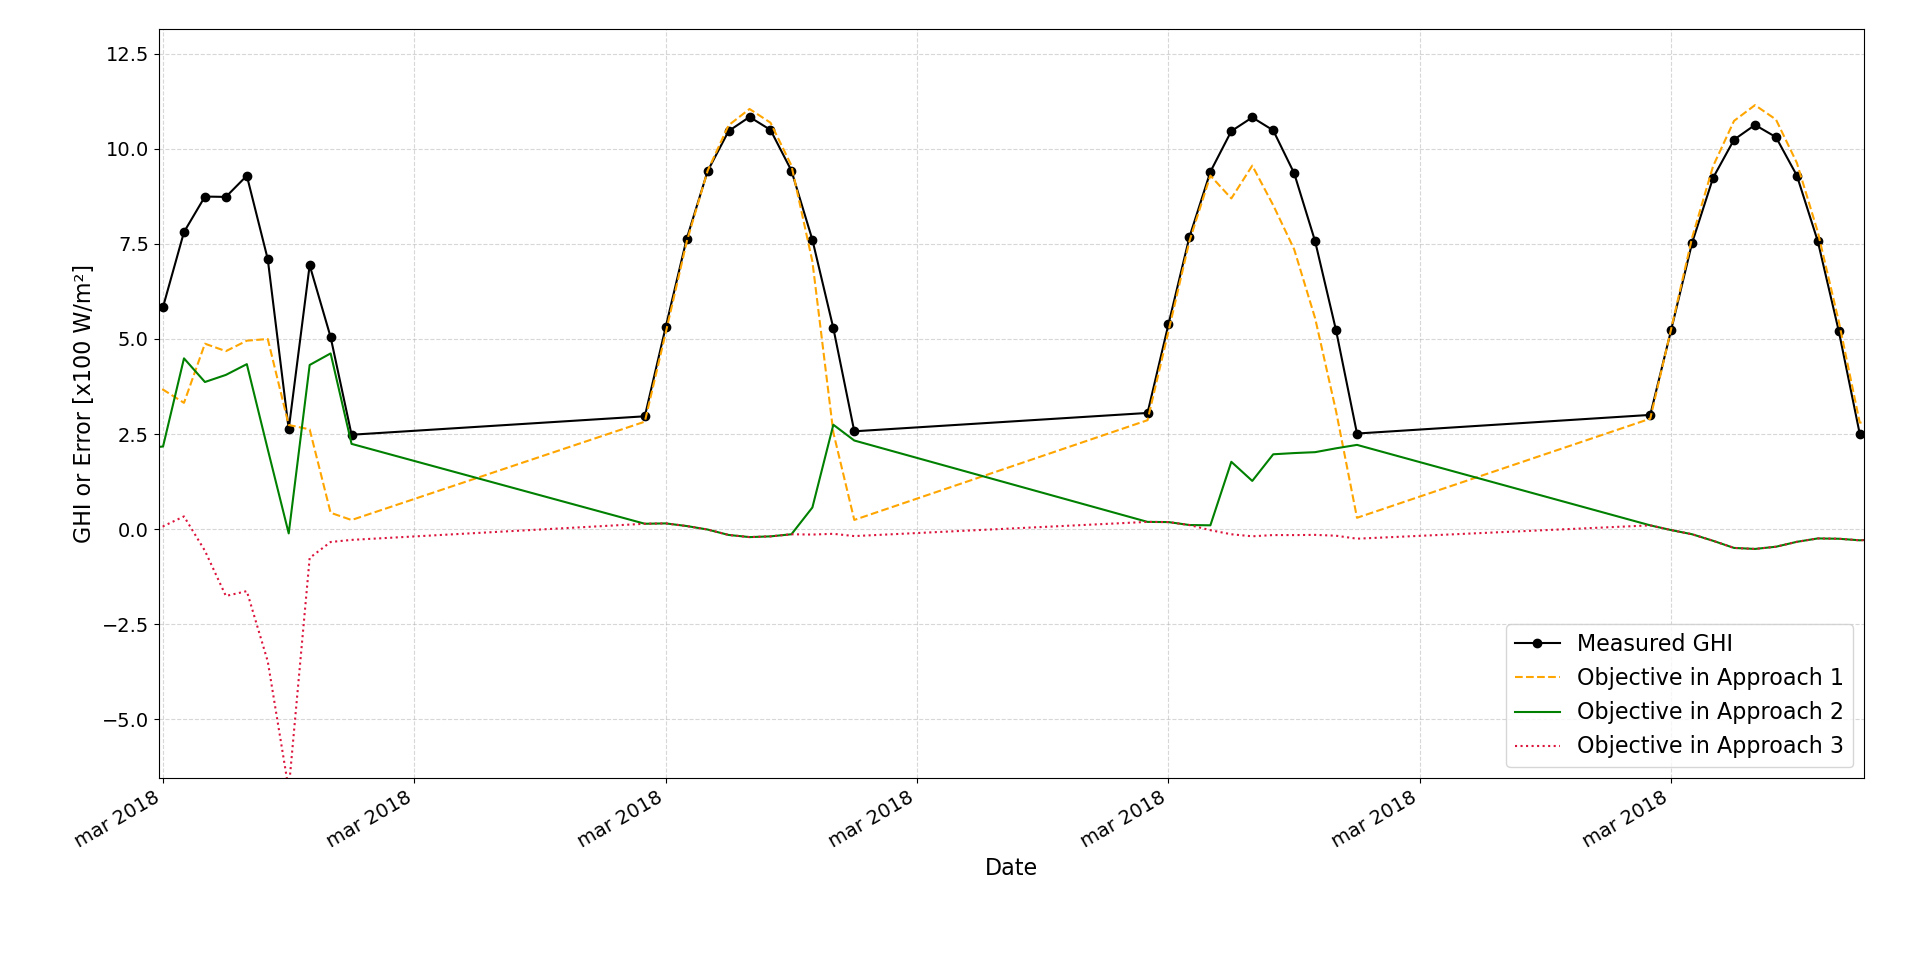
\includegraphics[width=\textwidth]{figuras/approaches.png}
%DIFDELCMD < %%%
%DIFDELCMD < \caption{%
{%DIFAUXCMD
\DIFdelFL{Diferencias entre los tres enfoques de adaptación.}}
%DIFAUXCMD
%DIFDELCMD < \label{fig:approaches}
%DIFDELCMD < \end{figure*}
%DIFDELCMD < 

%DIFDELCMD < %%%
\DIFdel{Los resultados obtenidos para cada uno de estos enfoques se presentan en la Tabla T. Cabe destacar que el Enfoque 1 fue es el evaluado en las secciones anteriores en esta tesis; para facilitar una comparación, se ha incluido también el reporte de las métricas correspondientes a este enfoque.
}%DIFDELCMD < 

%DIFDELCMD < \begin{table*}
%DIFDELCMD < %%%
%DIFDELCMD < \caption[Métricas de desempeño para cada modelo en el conjunto de prubeas.]{%
{%DIFAUXCMD
\DIFdelFL{Métricas de desempeño (MBE, MAE, RMSE) para cada modelo en el conjunto de prubeas de los cinco sitios. Los valores están normalizados y expresados como porcentajes relativos a la media de GHI en cada sitio: 429.2~W/m$^2$ (Yu), 432.9~W/m$^2$ (Sa), 554.4~W/m$^2$ (Sca), 628.4~W/m$^2$ (Ero), y 648.7~W/m$^2$ (Lq). Los modelos etiquetados con ``(1 var.)'' indican adaptación al sitio realizada utilizando solo un regresor (CAMS o LSA-SAF).}}
%DIFAUXCMD
%DIFDELCMD < \label{tab:metricas_4_1}
%DIFDELCMD < \centering
%DIFDELCMD < \resizebox{\linewidth}{!}{
%DIFDELCMD < \def\arraystretch{1.5}
%DIFDELCMD < \begin{tabular}{cccccccccccccccc}
%DIFDELCMD < \hline
%DIFDELCMD <       & \multicolumn{3}{c}{Yu} & \multicolumn{3}{c}{Sa} & \multicolumn{3}{c}{Sca} & \multicolumn{3}{c}{Ero} & \multicolumn{3}{c}{Lq} \\
%DIFDELCMD < Modelo & MBE & MAE & RMSE & MBE & MAE & RMSE  & MBE & MAE & RMSE & MBE & MAE & RMSE & MBE & MAE & RMSE  \\
%DIFDELCMD < \hline
%DIFDELCMD < \multicolumn{16}{|c|}{\textit{Adaptación al sitio en Escala 15-Minutal}} \\
%DIFDELCMD < \hline
%DIFDELCMD < CAMS      & -0.2 & 17.4 & 27.2 & 3.9  & 23.4 & 33.7 & 2.6  & 21.8 & 29.8 & -23.6 & 27.6 & 40.9 & -6.9 & 16.5 & 25.8 \\
%DIFDELCMD < CAMS - E1 & -0.9 & 17.1 & 26.4 & 3.8  & 21.3 & 31.5 & -1.5 & 18.4 & 26.0 &  2.5  & 24.8 & 31.5 &  2.1 & 15.9 & 23.5 \\
%DIFDELCMD < CAMS - E2 & -0.9 & 17.1 & 26.4 & 3.8  & 21.3 & 31.5 & -1.5 & 18.4 & 26.0 &  2.5  & 24.8 & 31.5 &  2.1 & 15.9 & 23.5 \\
%DIFDELCMD < CAMS - E3 & -2   & 17.5 & 27.1 & 3.8  & 22.7 & 33.3 &  3.3 & 19.1 & 28.6 &  0.1  & 13.6 & 22   & 2.9  & 12.7 & 21.2 \\
%DIFDELCMD < 

%DIFDELCMD < \hline
%DIFDELCMD < LSA-SAF      & 7.6  & 16.5 & 25.5 & 17.9 & 27.4  & 39.4 & 13.1& 22.2 & 30.9  & -7.7 & 16.2 & 26.5 & 4   & 12.6 & 22.6 \\
%DIFDELCMD < LSA-SAF - E1 & -5.5 & 18.4 & 25   & 4.4  & 23.9  & 34.6 & 1   & 18   & 26.7  &  2.7 & 17.1 & 25.4 & 2.2 & 12.8 & 22.3 \\
%DIFDELCMD < LSA-SAF - E2 & -5.5 & 18.4 & 25   & 4.4  & 23.9  & 34.6 & 1   & 18   & 26.7  &  2.7 & 17.1 & 25.4 & 2.2 & 12.8 & 22.3 \\
%DIFDELCMD < LSA-SAF - E3 & -5.3 & 16.7 & 24.7 & 4.2  & 23.8  & 35.4 & 4.3 & 19.2 & 28.7  &  0.9 & 12.7 & 21.5 & 2.6 & 12.8 & 21.9 \\
%DIFDELCMD < 

%DIFDELCMD < \hline
%DIFDELCMD < \multicolumn{16}{|c|}{\textit{Adaptación al sitio en Escala Horaria}} \\
%DIFDELCMD < \hline
%DIFDELCMD < CAMS           & -0.1 & 15.2 & 23.5 & 4.0 & 20.9  & 29.3 & 3.0  & 19.7  & 26.1 & -23.6 & 26.6 & 39.3 & -4.8 & 14.5 & 21.6 \\
%DIFDELCMD < CAMS  - E1    &  -0.5 & 14.7 & 22.6 &  3.5 & 18.5 & 27.0 & -1.7 & 15.9 & 22.0  &  2.1 & 23.4  & 29.6 &  2.6 & 13.8 & 19.4 \\
%DIFDELCMD < CAMS  - E2    &  -0.5 & 14.7 & 22.6 &  3.5 & 18.5 & 27.0 & -1.7 & 15.9 & 22.0  &  2.1 & 23.4  & 29.6 &  2.6 & 13.8 & 19.4 \\
%DIFDELCMD < CAMS  - E3    &  1.2 & 15.2  & 23.4 &  3.5 & 20.2 & 29   & 3.7  & 17.2  & 25.3 &  0.5 & 12    & 19.6 &  0.9 & 10.4 & 16.3 \\
%DIFDELCMD < \hline
%DIFDELCMD < LSA-SAF      & 7.6  & 14.4 & 21.8  & 17.9 & 25.3   & 35.6 & 13.2 & 20.2 & 27.1 & -7.6 & 14.3 & 24 & 4.8 & 10.8 & 18.2 \\
%DIFDELCMD < LSA-SAF - E1 & 5.1  & 16.5 & 24    & 4.3 & 21.2 & 30.5 & 1.1 & 15.6 & 22.7 &   2.5 & 15.7 & 22.8 &  0.3 & 10.6 & 17.4 \\
%DIFDELCMD < LSA-SAF - E2 & 5.1  & 16.5 & 24    & 4.3 & 21.2 & 30.5 & 1.1 & 15.6 & 22.7 &   2.5 & 15.7 & 22.8 &  0.3 & 10.6 & 17.4 \\
%DIFDELCMD < LSA-SAF - E3 & 4.7  & 15.7 & 23.2  & 4.1 & 21.1 & 31.1 & 4.7 & 17.1 & 25.1 &   1.3 & 11.1 & 18.9 &   0  & 10.7 & 17 \\
%DIFDELCMD < \hline
%DIFDELCMD < ERA5         & 1.2  & 22.2 & 33.7 & 9.4 & 27.1 & 37.7 & 1.9  & 20.2 & 29.7 & -14.0 & 19.3 & 25.6 & -0.8  & 11.3 & 18.4 \\
%DIFDELCMD < ERA-5 - E1   & 2.7  & 22.6 & 33.7 & 6.4 & 26.5 & 36.9 & -6.4 & 20.1 & 29.1 & -0.6  & 15.4 & 21.4 &  2.1  & 11.6 & 18.4 \\
%DIFDELCMD < ERA-5 - E2   & 2.7  & 22.6 & 33.7 & 6.4 & 26.5 & 36.9 & -6.4 & 20.1 & 29.1 & -0.6  & 15.4 & 21.4 &  2.1  & 11.6 & 18.4 \\
%DIFDELCMD < ERA5  - E3   & 0.1  & 23.4 & 32.3 & 6.8 & 26.9 & 37.2 & 0.2  & 18.8 & 26.7 & -0.4  & 12.7 & 19.4 &   0.7 & 10.5 & 17 \\
%DIFDELCMD < 

%DIFDELCMD < \hline
%DIFDELCMD < MERRA-2      & 24.9 & 33.5 & 51.2 & 43.4 & 48.3 & 65.0 & 10.9 & 21.7 & 30.3 & -3.8  & 13.1 & 20.4 & 1.4  & 13.4 & 20.8 \\
%DIFDELCMD < MERRA-2 - E1 & -2.6 & 34.5 & 44   &  7.1 & 35.2 & 46.0 & -2.2 & 20.3 & 27.7 &  0.7 & 12.9  & 20.1 &  0.3 & 13.1 & 20.4 \\
%DIFDELCMD < MERRA-2 - E2 & -2.6 & 34.5 & 44   &  7.1 & 35.2 & 46.0 & -2.2 & 20.3 & 27.7 &  0.7 & 12.9  & 20.1 &  0.3 & 13.1 & 20.4 \\
%DIFDELCMD < MERRA-2 - E3 & -4.5 & 35.1 & 44   & 7.5  & 35.6 & 48.1 &  2.5 & 19.8 & 28.6 & 0.4  & 11.4  & 18.7 &-0.5  & 11.6 & 18.2 \\
%DIFDELCMD < 

%DIFDELCMD < \hline
%DIFDELCMD < \end{tabular}}
%DIFDELCMD < \end{table*}
%DIFDELCMD < 

%DIFDELCMD < %%%
\DIFdel{La Tabla \ref{tab:metricas_4_1} y la Figura \ref{fig:metricas_estacionalidad} muestran las métricas de desempeño obtenidas tras evaluar los tres enfoques sobre la desestacionalización de la serie. Se comparan las estimaciones satelitales originales (CAMS y LSA-SAF) con sus adaptaciones al sitio mediante los enfoques E1, E2 y E3. 
Cada subplot corresponde a una métrica distinta, y dentro de cada sitio se presentan primero los modelos basados en CAMS y luego, separados visualmente, los basados en LSA-SAF. 
}%DIFDELCMD < 

%DIFDELCMD < %%%
\DIFdel{El Enfoque 1, que aplica una regresión lineal simple sobre los valores modelados, tiende a funcionar de manera consistente cuando la relación entre la irradiancia modelada y la medida es aproximadamente lineal y estable a lo largo del tiempo. Sin embargo, puede ser menos efectivo en sitios donde existen patrones estacionales complejos o variaciones sistemáticas que no se capturan con una regresión simple. 
}%DIFDELCMD < 

%DIFDELCMD < %%%
\DIFdel{El Enfoque 2, basado en modelar la diferencia entre el GHI medido y el modelado, permite ajustar directamente el error sistemático y suele mejorar el desempeño en sitios donde el sesgo del modelo es relativamente constante, pero puede fallar si las diferencias presentan fuerte dependencia estacional o si los errores son heterocedásticos a lo largo del año.
}%DIFDELCMD < 

%DIFDELCMD < %%%
\DIFdel{Finalmente, el Enfoque 3, que desestacionaliza tanto la variable regresora como la objetivo usando el GHI de cielo despejado, permite capturar patrones estacionales más complejos y corregir errores dependientes del ciclo solar diario y anual. Esto explica por qué, en general, presenta mejores métricas de rMAE y rRMSE en sitios con alta variabilidad estacional, como Ero y Lq, donde los enfoques anteriores muestran limitaciones.}%DIFDELCMD < \\
%DIFDELCMD < 

%DIFDELCMD < \begin{figure}
%DIFDELCMD <     \centering
%DIFDELCMD <     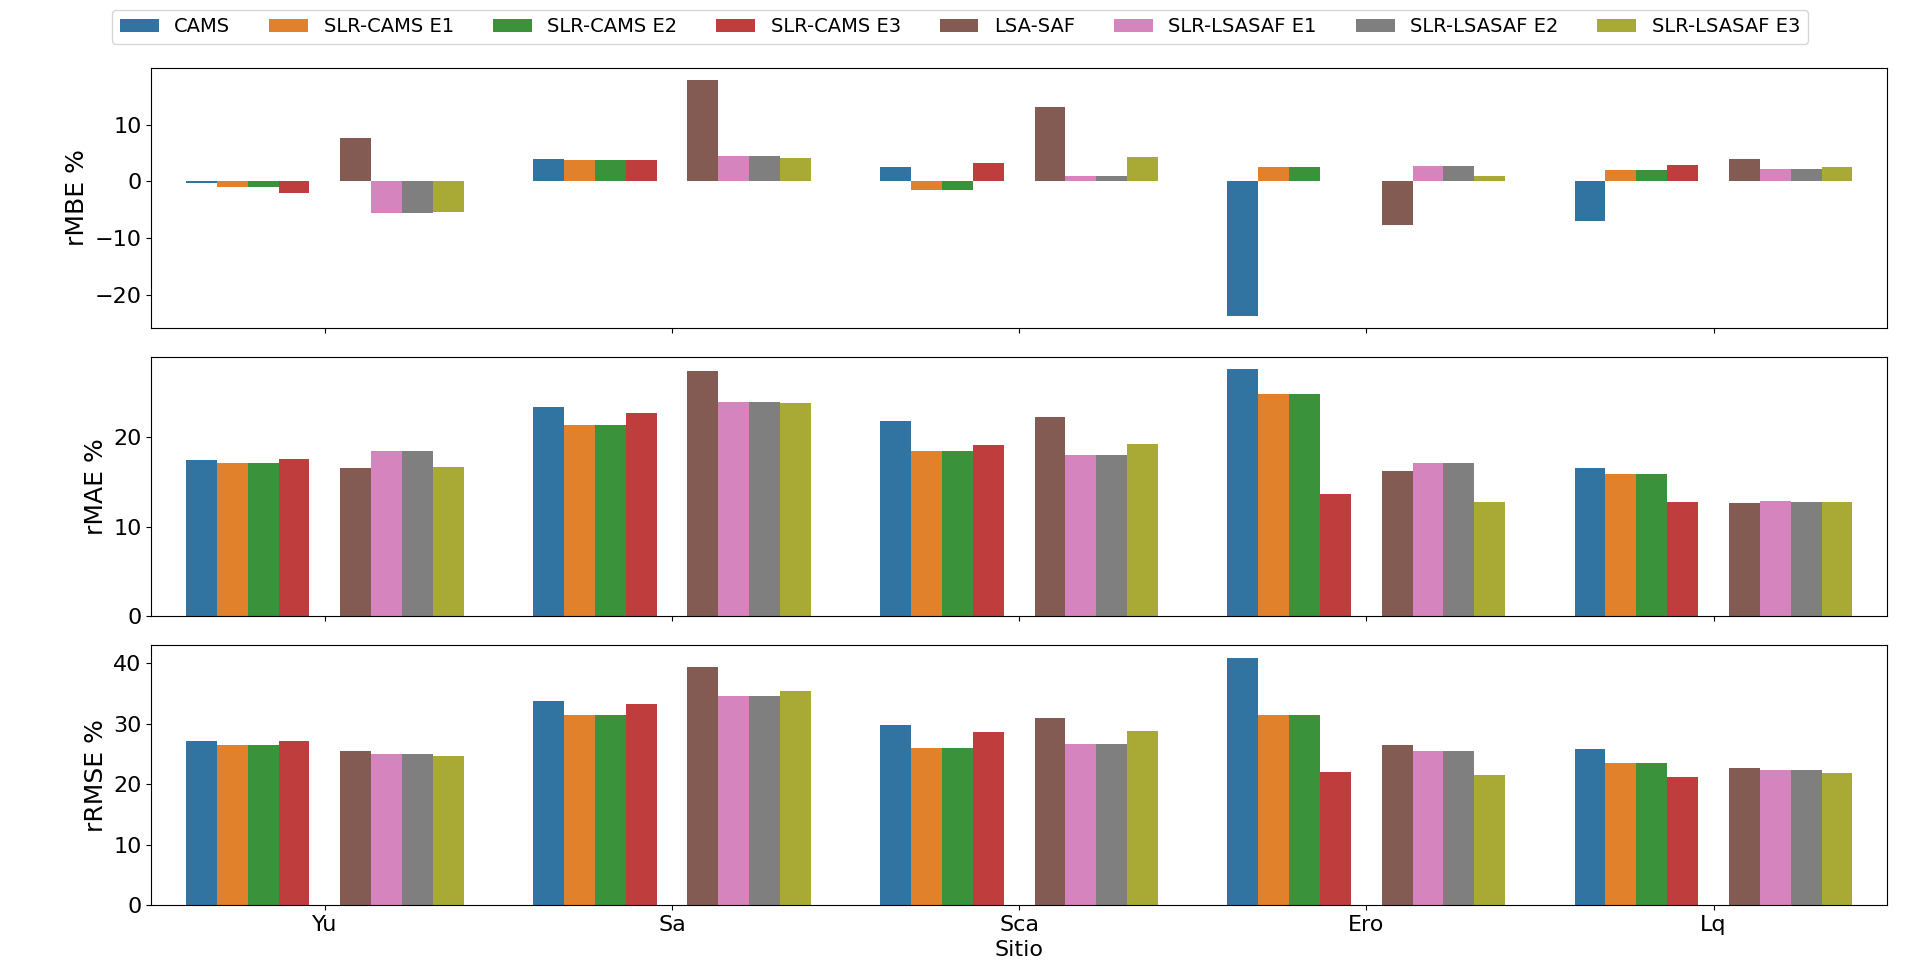
\includegraphics[width=\textwidth]{errors_estacionalidad.png}
%DIFDELCMD <     %%%
%DIFDELCMD < \caption[Métricas de desempeño para las estimaciones y sus adaptaciones midantes los enfoques E1, E2 y E3 ]{%
{%DIFAUXCMD
\DIFdelFL{Métricas de desempeño relativas (\textit{rMBE}, \textit{rMAE} y \textit{rRMSE}, en \%) obtenidas en los cinco sitios de prueba (Yu, Sa, Sca, Ero y Lq). 
    Se comparan las estimaciones satelitales originales (CAMS y LSA-SAF) con sus adaptaciones al sitio mediante los enfoques E1, E2 y E3. 
    En cada subplot se agrupan las barras por sitio, mostrando primero los modelos basados en CAMS y luego, separados visualmente, los modelos basados en LSA-SAF.}}
    %DIFAUXCMD
%DIFDELCMD < \label{fig:metricas_estacionalidad}
%DIFDELCMD < \end{figure}
%DIFDELCMD < 

%DIFDELCMD < %%%
\DIFdel{La Tabla \ref{tab:metricas_4_1} y la Figura \ref{fig:metricas_estacionalidad} muestran las métricas de desempeño obtenidas tras evaluar los tres enfoques sobre la desestacionalización de la serie. Se comparan las estimaciones satelitales originales (CAMS y LSA-SAF) con sus adaptaciones al sitio mediante los enfoques E1, E2 y E3. Cada subplot corresponde a una métrica distinta, y dentro de cada sitio se presentan primero los modelos basados en CAMS y luego, separados visualmente, los basados en LSA-SAF.
}%DIFDELCMD < 

%DIFDELCMD < %%%
\DIFdel{Los resultados muestran que los Enfoques 1 y 2 producen métricas idénticas, lo cual confirma que, bajo un modelo de regresión lineal simple, ambas formulaciones son matemáticamente equivalentes. Esta equivalencia implica que, en contextos donde las diferencias entre las estimaciones modeladas y medidas se comportan de manera lineal y sin dependencia temporal significativa, cualquiera de los dos enfoques puede emplearse sin pérdida de precisión. Sin embargo, en escenarios donde la estacionalidad o las fluctuaciones no lineales del error adquieren un papel preponderante, estos enfoques resultan insuficientes para capturar las variaciones sistemáticas de la irradiancia a lo largo del año.
}%DIFDELCMD < 

%DIFDELCMD < %%%
\DIFdel{En contraste, el Enfoque 3 introduce una capa adicional de análisis al incorporar la desestacionalización mediante el uso del GHI en condiciones de cielo despejado. Este procedimiento permite aislar la componente física más estable de la señal —aquella asociada principalmente a la geometría solar y a la variación predecible de la posición del Sol— y concentrar la regresión sobre las fluctuaciones residuales de origen atmosférico, tales como las asociadas a la nubosidad p los aerosoles. En otras palabras, al eliminar la variabilidad periódica causada por los ciclos diurnos y estacionales, el modelo deja de ajustar su salida sobre un patrón medio predecible y pasa a aprender cómo responden las desviaciones locales del GHI ante cambios reales en las condiciones atmosféricas. Esto permite que la regresión capture mejor los fenómenos de corto plazo que explican las diferencias entre la irradiancia ideal y la medida en cada sitio.
}%DIFDELCMD < 

%DIFDELCMD < %%%
\DIFdel{Este enfoque resulta particularmente valioso en regiones donde la variabilidad estacional es marcada, como se observa en los sitios Ero y Lq, donde los ciclos anuales de nubosidad y carga de aerosoles introducen sesgos significativos en las estimaciones satelitales. Al remover la tendencia estacional, el modelo adquiere mayor capacidad para identificar patrones de corto plazo, mejorando la respuesta frente a fenómenos transitorios. Además, la linealidad preservada en la formulación permite una interpretación directa de los coeficientes $a$ y $b$, facilitando la evaluación física de los ajustes realizados sobre la irradiancia modelada.
}%DIFDELCMD < 

%DIFDELCMD < %%%
\DIFdel{La principal ventaja de utilizar un modelo interpretable radica en que permite comprender la naturaleza del ajuste aplicado a las estimaciones originales. En contextos meteorológicos y energéticos, esta interpretabilidad tiene implicancias prácticas: por ejemplo, conocer el valor del coeficiente de escala ($a$) y del sesgo aditivo ($b$) puede indicar si el modelo satelital tiende a sobrestimar o subestimar sistemáticamente la irradiancia bajo determinadas condiciones atmosféricas. Tal información es crucial para la calibración de sistemas de predicción solar o para la transferencia de modelos entre sitios con características climáticas similares.
}%DIFDELCMD < 

%DIFDELCMD < %%%
\DIFdel{Además, mantener la estructura lineal del proceso de adaptación facilita la integración del modelo en sistemas operativos o plataformas de monitoreo en tiempo real, donde la simplicidad computacional y la transparencia en la interpretación son factores determinantes. A diferencia de los modelos basados en redes neuronales profundas o enfoques de caja negra, los métodos lineales desestacionalizados permiten identificar de manera explícita cómo se corrigen los errores sistemáticos, lo cual incrementa la confiabilidad del modelo en aplicaciones críticas como la gestión de recursos energéticos o la validación de productos satelitales.
}%DIFDELCMD < 

%DIFDELCMD < %%%
\DIFdel{No obstante, es importante señalar que la desestacionalización basada exclusivamente en el GHI de cielo despejado representa solo una de las posibles estrategias para abordar la no estacionariedad. Existen alternativas complementarias que podrían ser exploradas en trabajos futuros, tales como el filtrado de series mediante transformadas de Fourier, la descomposición empírica en modos (EMD), o la descomposición estacional mediante técnicas de suavizado loess (STL). Estas metodologías permiten capturar variaciones estacionales de diferente naturaleza y frecuencia, adaptándose mejor a contextos con patrones no periódicos o con transiciones abruptas de nubosidad.
}%DIFDELCMD < 

%DIFDELCMD < %%%
\DIFdel{Asimismo, enfoques híbridos que combinen desestacionalización con técnicas multiescala —por ejemplo, mediante transformadas wavelet discretas— pueden ofrecer una descripción más detallada de las dinámicas locales de la irradiancia. Al descomponer la señal en distintos niveles de resolución temporal, es posible diferenciar entre componentes de variabilidad diaria, sinótica o estacional, lo que podría mejorar la robustez de la adaptación al sitio en entornos climáticamente heterogéneos. Estas estrategias también permitirían evaluar la sensibilidad del proceso de corrección frente a distintos horizontes temporales, proporcionando un marco más generalizable.
}%DIFDELCMD < 

%DIFDELCMD < %%%
\DIFdel{Desde una perspectiva metodológica, incorporar una etapa de desestacionalización dentro del proceso de adaptación al sitio representa una evolución conceptual hacia modelos físicamente fundamentados y estadísticamente coherentes. Este paso no solo mejora las métricas de error, sino que contribuye a la construcción de modelos más generalizables, capaces de transferirse entre regiones o periodos de tiempo sin requerir una recalibración exhaustiva. De hecho, la separación explícita entre las componentes estacionales y residuales puede considerarse una práctica recomendable en cualquier modelización de series meteorológicas con dependencia temporal marcada.
}%DIFDELCMD < 

%DIFDELCMD < %%%
\DIFdel{Finalmente, el enfoque propuesto reafirma la idea de que la simplicidad y la interpretabilidad no son incompatibles con la precisión. Al contrario, un modelo lineal correctamente estructurado, apoyado por un tratamiento temporal adecuado de la serie, puede alcanzar un rendimiento comparable o superior al de modelos más complejos. Esto tiene profundas implicancias en la modelización de irradiancia: permite conservar la trazabilidad física de las variables, facilita la transferencia del conocimiento entre dominios geográficos y reduce la opacidad de los procesos de ajuste, todo ello sin sacrificar capacidad predictiva. En conjunto, la desestacionalización integrada dentro del proceso de adaptación al sitio constituye una alternativa sólida, transparente y científicamente defendible para mejorar las estimaciones de GHI a partir de productos satelitales o de reanálisis.
}%DIFDELCMD < 

%DIFDELCMD < %%%
\section{\DIFdel{Validación cruzada de los modelos de adaptación al sitio}}
%DIFAUXCMD
\addtocounter{section}{-1}%DIFAUXCMD
%DIFDELCMD < 

%DIFDELCMD < %%%
\DIFdel{En las secciones anteriores se evaluaron distintos enfoques de adaptación al sitio, evidenciando el potencial de este proceso según las características del modelo de estimación y del sitio donde se aplique. Sin embargo, cada uno de los enfoques fue probado únicamente en el mismo sitio en el que se ajustó, siguiendo así el esquema tradicional de adaptación al sitio. Con el fin de analizar la capacidad de generalización espacial de los modelos, se propuso un procedimiento de \textbf{validación cruzada entre sitios}, en el cual los modelos entrenados en una estación se aplican a otras geográficamente distintas.
}%DIFDELCMD < 

%DIFDELCMD < %%%
\DIFdel{Este procedimiento permite evaluar la habilidad del modelo para mantener un desempeño adecuado fuera del entorno donde fue calibrado originalmente. En otras palabras, mide la capacidad del modelo para reproducir patrones en sitios con condiciones ambientales diferentes, lo que resulta fundamental para el desarrollo de productos regionales o mapas climáticos derivados de la adaptación al sitio. En estos contextos, se busca minimizar la dependencia de calibraciones locales, aprovechando patrones espaciales comunes que mejoren la consistencia regional del modelo.
}%DIFDELCMD < 

%DIFDELCMD < \begin{figure}[H]
%DIFDELCMD < \centering
%DIFDELCMD < \begin{subfigure}[b]{0.48\textwidth}
%DIFDELCMD < \centering
%DIFDELCMD < 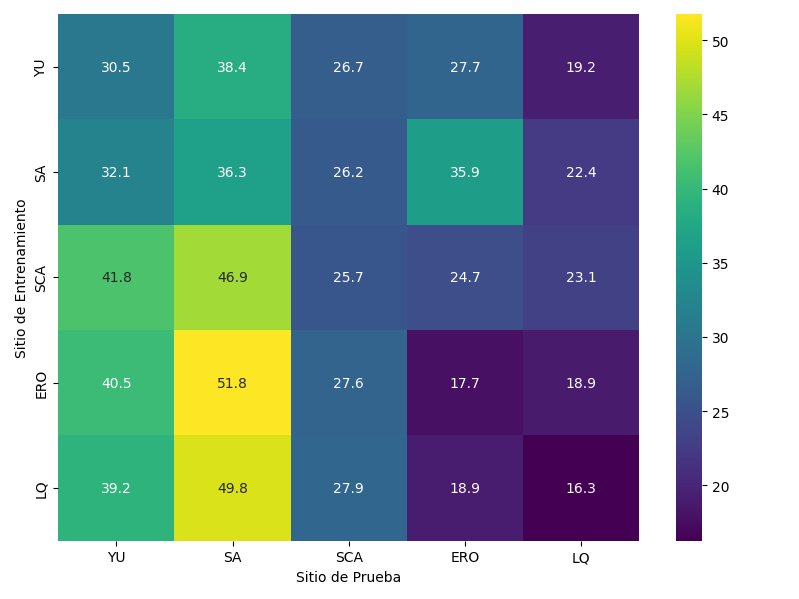
\includegraphics[width=\textwidth]{figuras/CrossValidationOneSite.png}
%DIFDELCMD < %%%
%DIFDELCMD < \caption{%
{%DIFAUXCMD
\DIFdelFL{Matriz de rRMSE (\%) obtenida a partir de la validación cruzada entre sitios para el modelo ERA5, utilizando los modelos ajustados con celdas satelitales adyacentes al sitio de interés.}}
%DIFAUXCMD
%DIFDELCMD < \label{fig:crossValidation}
%DIFDELCMD < \end{subfigure}
%DIFDELCMD < \hfill
%DIFDELCMD < \begin{subfigure}[b]{0.48\textwidth}
%DIFDELCMD < \centering
%DIFDELCMD < 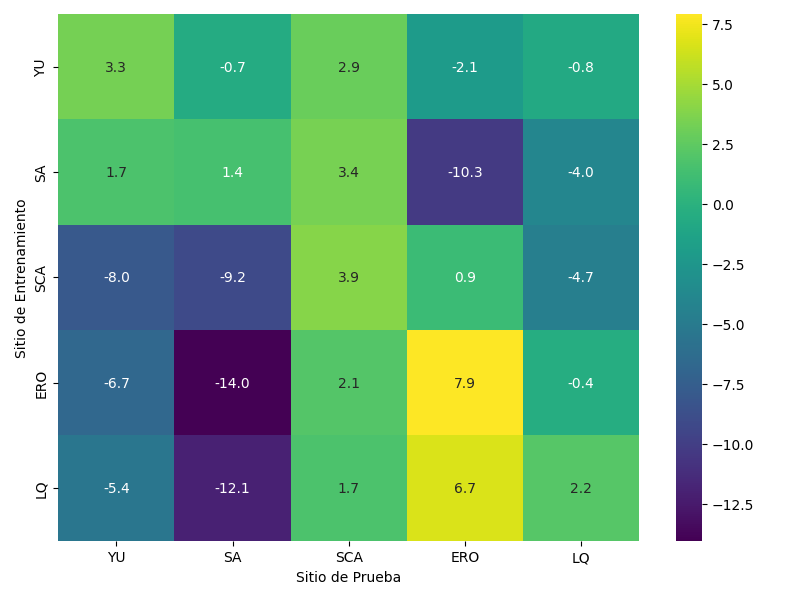
\includegraphics[width=\textwidth]{figuras/DeltaCrossValidationOneSite.png}
%DIFDELCMD < %%%
%DIFDELCMD < \caption{%
{%DIFAUXCMD
\DIFdelFL{Diferencia en desempeño entre el modelo sin ajustar (ERA5 original) y el modelo adaptado a cada sitio. Cada fila indica el sitio de entrenamiento y cada columna el sitio de prueba.}}
%DIFAUXCMD
%DIFDELCMD < \label{fig:deltaCrossValidation}
%DIFDELCMD < \end{subfigure}
%DIFDELCMD < %%%
%DIFDELCMD < \caption{%
{%DIFAUXCMD
\DIFdelFL{Resultados de la validación cruzada entre sitios para el modelo ERA5.}}
%DIFAUXCMD
%DIFDELCMD < \label{fig:crossValidationAll}
%DIFDELCMD < \end{figure}
%DIFDELCMD < 

%DIFDELCMD < %%%
\DIFdel{La Figura \ref{fig:crossValidation} presenta la matriz de sensibilidad del rRMSE (\%) obtenida a partir de las validaciones cruzadas entre los distintos sitios, mientras que la Figura \ref{fig:deltaCrossValidation} muestra la diferencia en el desempeño relativo entre el modelo ERA5 original y los modelos adaptados mediante regresión múltiple (MLR). En cada matriz, las filas representan los sitios de entrenamiento y las columnas los sitios de prueba, permitiendo identificar las relaciones de transferencia entre ubicaciones.
}%DIFDELCMD < 

%DIFDELCMD < %%%
\DIFdel{Los resultados evidencian un aumento del error cuando los modelos son aplicados en sitios con características ambientales distintas de aquellas en las que fueron entrenados. Este comportamiento confirma que la capacidad de extrapolación espacial de los modelos de adaptación al sitio es limitada y depende fuertemente de la similitud climática y topográfica entre estaciones. En particular, los modelos ajustados en sitios de baja altitud presentan un mejor desempeño en zonas con condiciones altitudinales similares, mientras que su transferencia a regiones de mayor altura suele degradar el rendimiento. De manera opuesta, los modelos entrenados en sitios de alta montaña muestran mayor robustez cuando se aplican en otros sitios con altitudes comparables, lo que sugiere que la altitud actúa como una variable determinante en la estructura térmica y la humedad del aire, influyendo directamente en la radiación solar incidente.
}%DIFDELCMD < 

%DIFDELCMD < %%%
\DIFdel{Asimismo, se observó que algunos sitios actúan como \textit{donantes más universales}, cuyos modelos presentan una capacidad de transferencia más amplia. Identificar estos sitios resulta esencial para optimizar la calibración regional y reducir la necesidad de ajustes locales independientes. En contraste, los valores negativos en la matriz $\Delta \text{rRMSE}$ reflejan casos donde la adaptación no solo no mejora, sino que empeora el desempeño, posiblemente debido a sobreajustes locales o a la falta de representatividad espacial de las variables predictoras. De manera general, se concluye que la transferencia entre sitios es direccional y asimétrica: un modelo entrenado en un sitio A puede funcionar adecuadamente en un sitio B, pero no necesariamente a la inversa, dependiendo de las características climáticas y de variabilidad regional de cada zona.
}%DIFDELCMD < 

%DIFDELCMD < %%%
\DIFdel{Estos resultados permiten establecer que la validación cruzada entre sitios constituye una herramienta fundamental para definir el grado de representatividad espacial de los modelos de adaptación. A partir de este análisis, se puede determinar qué ajustes locales son transferibles a áreas vecinas y cuáles requieren una recalibración específica. En consecuencia, para la construcción de mapas regionales \textit{site-adapted}, se propone una estrategia de generalización basada en el uso combinado de la información geográfica y de la similitud ambiental.
}%DIFDELCMD < 

%DIFDELCMD < %%%
\subsection*{\DIFdel{Propuesta de generalización basada en distancia geográfica y altitud}}
%DIFAUXCMD
%DIFDELCMD < 

%DIFDELCMD < %%%
\DIFdel{Considerando los resultados anteriores, se propone un enfoque de \textbf{generalización espacial automática}, destinado a extender los modelos ajustados hacia puntos donde no existen mediciones directas. La idea central consiste en asignar, a cada celda del dominio de interés, el modelo de regresión correspondiente a la estación más cercana, evaluando la \textbf{distancia euclídea tridimensional} entre cada punto de la grilla y las estaciones de referencia. 
}%DIFDELCMD < 

%DIFDELCMD < %%%
\DIFdel{Esta distancia se calcula combinando las coordenadas geográficas (latitud y longitud) junto con la altitud, de modo que el criterio de proximidad no sea únicamente horizontal, sino también vertical, incorporando la influencia del relieve sobre la radiación solar. 
}%DIFDELCMD < 

%DIFDELCMD < %%%
\DIFdel{Para asegurar que las tres variables contribuyan de forma comparable al cálculo de la distancia, todas las coordenadas son previamente \textbf{normalizadas mediante una transformación tipo z-score}, restando su media y dividiendo por la desviación estándar según la distribución espacial del dominio. Esta normalización evita que las diferencias de escala entre unidades —grados para latitud/longitud y metros para altitud— distorsionen la medida de proximidad y permite que la altitud tenga un peso equivalente al de las dimensiones horizontales. 
}%DIFDELCMD < 

%DIFDELCMD < %%%
\DIFdel{El proceso de normalización se expresa como:
}%DIFDELCMD < 

%DIFDELCMD < %%%
\[
\DIFdel{x' = \frac{x - \bar{x}}{\sigma_x}, \quad
y' = \frac{y - \bar{y}}{\sigma_y}, \quad
z' = \frac{z - \bar{z}}{\sigma_z}
}\]%DIFAUXCMD
%DIFDELCMD < 

%DIFDELCMD < \noindent %%%
\DIFdel{donde $\bar{x}$, $\bar{y}$ y $\bar{z}$ representan las medias, y $\sigma_x$, $\sigma_y$, $\sigma_z$ las desviaciones estándar de cada variable en la grilla de alta resolución. Posteriormente, la distancia entre un punto $P(x', y', z')$ y una estación $S_i(x_i', y_i', z_i')$ se define como:
}%DIFDELCMD < 

%DIFDELCMD < %%%
\[
\DIFdel{D_i = \sqrt{(x' - x_i')^2 + (y' - y_i')^2 + (z' - z_i')^2}
}\]%DIFAUXCMD
%DIFDELCMD < 

%DIFDELCMD < %%%
\DIFdel{El modelo asignado a cada celda corresponde al de la estación que minimiza esta distancia, es decir, el modelo con mayor similitud espacial y altitudinal con el punto de interés. Un esquema que ejemplifica esta propuesta se presenta en la Figura \ref{fig:distancias}.
}%DIFDELCMD < 

%DIFDELCMD < \begin{figure}
%DIFDELCMD <     \centering
%DIFDELCMD <     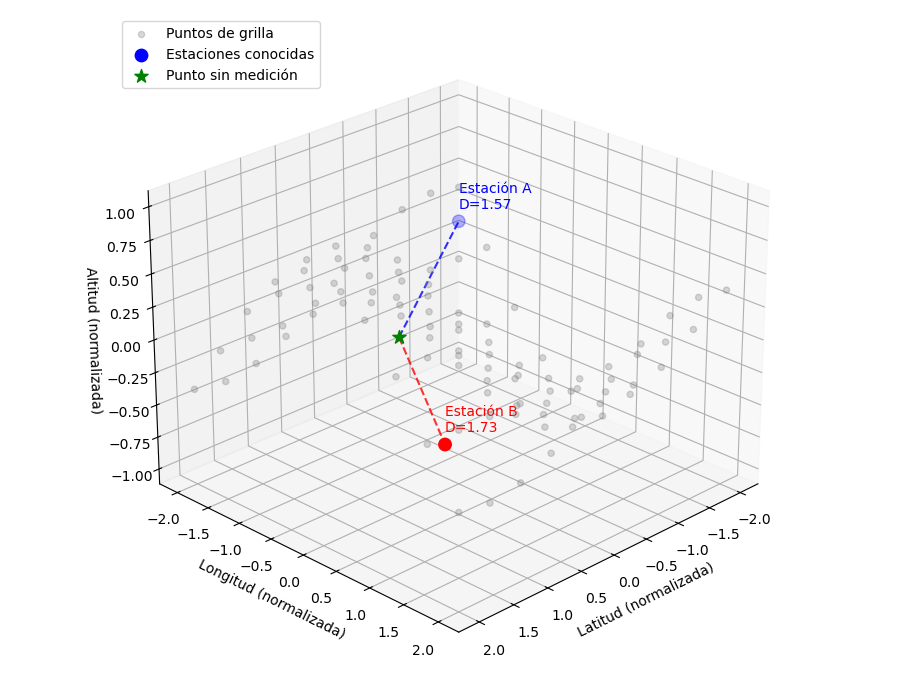
\includegraphics[width=\textwidth]{distancia3d.png}
%DIFDELCMD <     %%%
%DIFDELCMD < \caption[Ejemplo de asignación por distancia geográfica y altitudinal.]{%
{%DIFAUXCMD
\DIFdelFL{Ejemplo de asignación por distancia geográfica y altitudinal (normalizada). En gris se representan los puntos donde se pretende aplicar la generalización (sin medición). Los puntos azul y rojo indican estaciones A y B (con medición directa). En verde se muestra el punto objetivo sin medición, que recibe el modelo de la estación más cercana. Las líneas punteadas indican las distancias tridimensionales calculadas tras la normalización, señalando cuál de ellas es menor (la que define el modelo asignado).}}
    %DIFAUXCMD
%DIFDELCMD < \label{fig:distancias}
%DIFDELCMD < \end{figure}
%DIFDELCMD < 

%DIFDELCMD < %%%
\DIFdel{En la práctica, este procedimiento se implementó utilizando un árbol de búsqueda espacial (\texttt{KD-Tree}), que permite determinar de manera eficiente la estación más cercana a cada celda del dominio. De esta forma, cada punto recibe el modelo de regresión que mejor representa sus condiciones geográficas y topográficas. Este criterio de generalización permite integrar la altitud como variable de similitud, garantiza la continuidad espacial del campo corregido evitando discontinuidades entre zonas dominadas por distintos modelos, y permite escalar el enfoque a dominios amplios sin requerir calibraciones locales adicionales. En síntesis, esta metodología combina la precisión de los ajustes locales con una asignación geográfica racional, posibilitando la construcción de mapas de radiación solar adaptados al sitio en toda la región de estudio, incluso en áreas sin observaciones directas.}%DIFDELCMD < \\
%DIFDELCMD < 

%DIFDELCMD < %%%
\DIFdel{Siguiendo este criterio, se evaluaron los modelos ajustados en dos sitios para las estimaciones de ERA5. La información correspondiente se presenta en la Tabla \ref{tab:sites-testeo}. 
}%DIFDELCMD < 

%DIFDELCMD < \begin{table}
%DIFDELCMD <     \centering
%DIFDELCMD <     \renewcommand{\arraystretch}{1.5}
%DIFDELCMD <     \begin{tabular}{|>{\centering\arraybackslash}p{2cm}|>{\centering\arraybackslash}p{2cm}|>{\centering\arraybackslash}p{2cm}|>{\centering\arraybackslash}p{2cm}|>{\centering\arraybackslash}p{2cm}|>{\centering\arraybackslash}p{2cm}|>{\centering\arraybackslash}p{2cm}|}
%DIFDELCMD <         \hline
%DIFDELCMD <         %%%
\DIFdelFL{\textbf{ID} }%DIFDELCMD < & %%%
\DIFdelFL{\textbf{Provincia} }%DIFDELCMD < & %%%
\DIFdelFL{\textbf{Localidad} }%DIFDELCMD < & %%%
\DIFdelFL{\textbf{Latitud} }%DIFDELCMD < & %%%
\DIFdelFL{\textbf{Longitud} }%DIFDELCMD < & %%%
\DIFdelFL{\textbf{Altitud (m s.n.m.)} }%DIFDELCMD < & %%%
\DIFdelFL{\textbf{Clima}}%DIFDELCMD < \\ 
%DIFDELCMD <         \hline
%DIFDELCMD <         %%%
\DIFdelFL{\textbf{Ap} }%DIFDELCMD < & %%%
\DIFdelFL{Jujuy }%DIFDELCMD < & %%%
\DIFdelFL{Abra Pampa }%DIFDELCMD < & %%%
\DIFdelFL{-22.80 }%DIFDELCMD < & %%%
\DIFdelFL{-65.82 }%DIFDELCMD < & %%%
\DIFdelFL{3459 }%DIFDELCMD < & %%%
\DIFdelFL{\textbf{Cwa}}%DIFDELCMD < \\ 
%DIFDELCMD <         %%%
\DIFdelFL{\textbf{Ce} }%DIFDELCMD < & %%%
\DIFdelFL{Salta }%DIFDELCMD < & %%%
\DIFdelFL{Cerrillos  }%DIFDELCMD < & %%%
\DIFdelFL{-24.89 }%DIFDELCMD < & %%%
\DIFdelFL{-65.47 }%DIFDELCMD < & %%%
\DIFdelFL{1233 }%DIFDELCMD < & %%%
\DIFdelFL{\textbf{Cwb}}%DIFDELCMD < \\ 
%DIFDELCMD <         \hline    
%DIFDELCMD <     \end{tabular}
%DIFDELCMD <     %%%
%DIFDELCMD < \caption{%
{%DIFAUXCMD
\DIFdelFL{Estaciones de medida utilizadas para la validación de los modelos ajustados.}}
    %DIFAUXCMD
%DIFDELCMD < \label{tab:sites-testeo}
%DIFDELCMD < \end{table}
%DIFDELCMD < 

%DIFDELCMD < %%%
\DIFdel{Ambas estaciones pertenecen a la extinta red Enarsol, y los datos utilizados corresponden al año 2017. Aplicando el criterio de generalización espacial propuesto, se determina que el modelo de regresión a utilizar en Abra Pampa (Ap) corresponde al calibrado en la estación Lq, debido a la similitud altitudinal predominante, mientras que para Cerrillos (Ce) se debe aplicar el modelo calibrado en Sa, que presenta características geográficas y altitudinales comparables.
}%DIFDELCMD < 

%DIFDELCMD < \begin{table*}
%DIFDELCMD < %%%
%DIFDELCMD < \caption[Métricas de desempeño para el modelo ERA5 en los sitios de validación.]{%
{%DIFAUXCMD
\DIFdelFL{Métricas de desempeño (MBE, MAE, RMSE) para el modelo ERA5 en los sitios de validación. Los valores están normalizados y expresados como porcentajes relativos a la media de GHI en cada sitio: 429.2~W/m$^2$ (Ap), 432.9~W/m$^2$ (Ce).}}
%DIFAUXCMD
%DIFDELCMD < \label{tab:metricas_5}
%DIFDELCMD < \centering
%DIFDELCMD < \resizebox{\linewidth}{!}{
%DIFDELCMD < \begin{tabular}{ccccccc}
%DIFDELCMD < \hline
%DIFDELCMD <       & \multicolumn{3}{c}{Ap} & \multicolumn{3}{c}{Ce} \\
%DIFDELCMD < \textbf{Modelo} & \textbf{MBE} & \textbf{MAE} & \textbf{RMSE}  & \textbf{MBE} & \textbf{MAE} & \textbf{RMSE}  \\
%DIFDELCMD < \hline
%DIFDELCMD < ERA5          & 2.6 & 11.2 & 19.7 & 13.4 & 27.0 & 38.1  \\
%DIFDELCMD < ERA5 Ajustado & 1.8 & 11.2 & 19.6 & 7.8  & 25.2 & 36.5\\
%DIFDELCMD < \hline
%DIFDELCMD < \end{tabular}}
%DIFDELCMD < \end{table*}
%DIFDELCMD < 

%DIFDELCMD < \begin{figure}
%DIFDELCMD < \centering
%DIFDELCMD < \begin{subfigure}[b]{0.48\textwidth}
%DIFDELCMD < \centering
%DIFDELCMD < 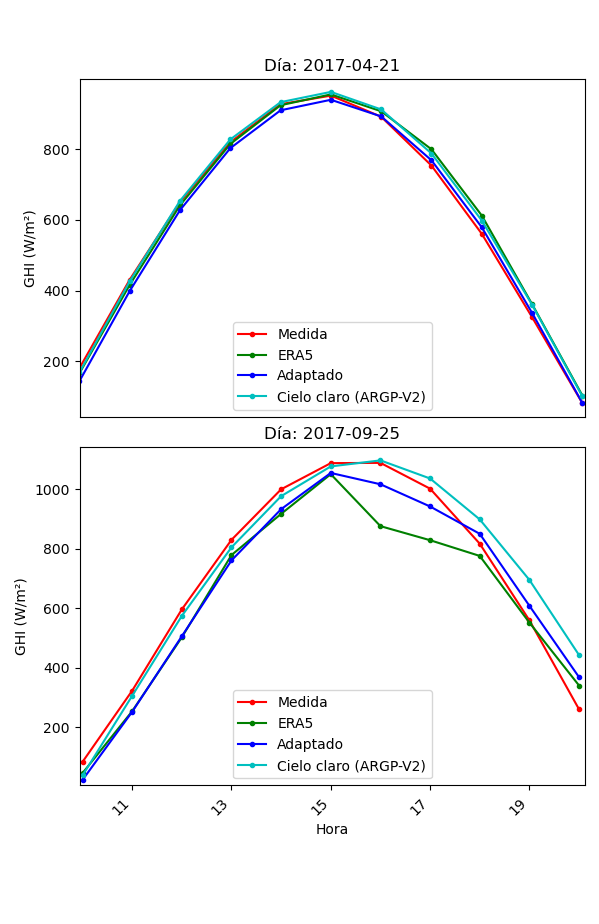
\includegraphics[width=\textwidth]{figuras/AP_corregido.png}
%DIFDELCMD < %%%
%DIFDELCMD < \caption{%
{%DIFAUXCMD
}
%DIFAUXCMD
%DIFDELCMD < \label{fig:validacionAP}
%DIFDELCMD < \end{subfigure}
%DIFDELCMD < \hfill
%DIFDELCMD < \begin{subfigure}[b]{0.48\textwidth}
%DIFDELCMD < \centering
%DIFDELCMD < 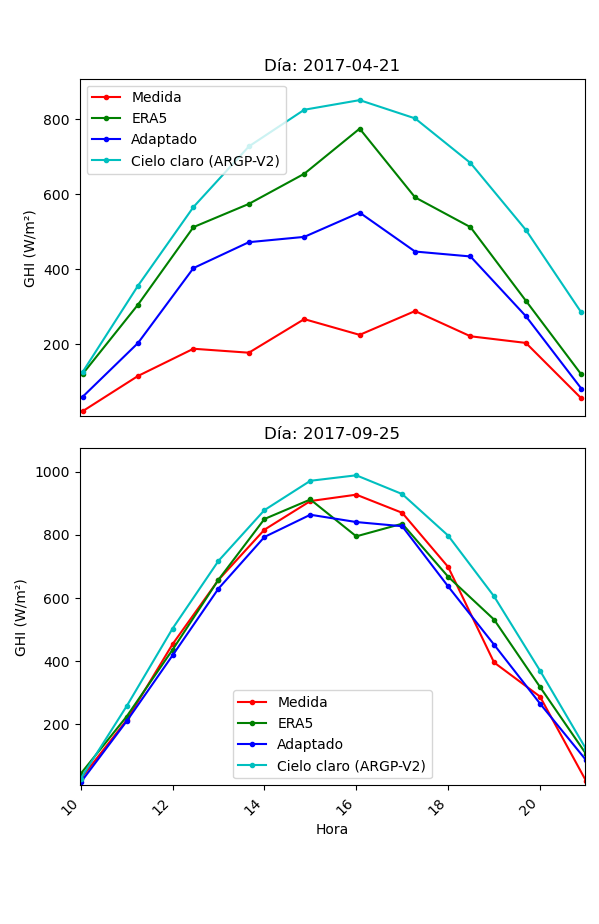
\includegraphics[width=\textwidth]{CE_corregido.png}
%DIFDELCMD < %%%
%DIFDELCMD < \caption{%
{%DIFAUXCMD
}
%DIFAUXCMD
%DIFDELCMD < \label{fig:validacionCE}
%DIFDELCMD < \end{subfigure}
%DIFDELCMD < %%%
%DIFDELCMD < \caption[Comparación entre la GHI medida y la estimada mediante el criterio de generalización propuesto para ERA5 en los sitios Abra Pampa y Cerrillos.]{%
{%DIFAUXCMD
\DIFdelFL{Comparación entre la GHI medida y la estimada mediante el criterio de generalización propuesto para el reanálisis ERA5 en los sitios de Abra Pampa (a) y Cerrillos (b).}}
%DIFAUXCMD
%DIFDELCMD < \label{fig:validacion}
%DIFDELCMD < \end{figure}
%DIFDELCMD < 

%DIFDELCMD < %%%
\DIFdel{Los resultados presentados en la Tabla \ref{tab:metricas_5} y la Figura \ref{fig:validacion} muestran que la aplicación del enfoque de generalización basado en distancia tridimensional produce mejoras modestas pero consistentes en los indicadores de desempeño del modelo ERA5. En ambos sitios se observa una reducción del sesgo medio (MBE) respecto al modelo original, indicando que la adaptación local corrige parcialmente las desviaciones sistemáticas en la estimación de la radiación global. En términos de error medio absoluto (MAE) y raíz del error cuadrático medio (RMSE), las variaciones son menores pero reflejan una mejora general en la estabilidad del modelo adaptado.
}%DIFDELCMD < 

%DIFDELCMD < %%%
\DIFdel{En Abra Pampa, el desempeño del modelo ajustado se mantiene prácticamente inalterado respecto al original, lo cual sugiere que el modelo ERA5 ya reproduce adecuadamente la variabilidad de la radiación en regiones de considerable altitud como ocurre en Ero o Lq. No obstante, la ligera disminución del MBE confirma que el ajuste regional contribuye a compensar diferencias locales vinculadas a la altitud y las condiciones atmosféricas secas características del altiplano. En cambio, en Cerrillos, el impacto del ajuste es más evidente: se reduce el sesgo en más del 40\%.
}%DIFDELCMD < 

%DIFDELCMD < %%%
\DIFdel{De manera general, los resultados validan la utilidad del esquema de generalización espacial propuesto, indicando que la transferencia de modelos basada en distancia geográfica y altitud puede ser una estrategia eficaz para extender la adaptación al sitio a dominios sin observaciones directas. Aunque las mejoras cuantitativas son moderadas, la consistencia espacial lograda en los campos de radiación corregida representa un avance significativo hacia la construcción de productos regionales coherentes, con potencial para aplicaciones en modelado climático, energía solar y gestión ambiental.
}%DIFDELCMD < 

%DIFDELCMD <  \newpage  %%%
\DIFdelend \DIFaddbegin \include{Capitulo3} \DIFaddend %Obligatorio
\DIFdelbegin %DIFDELCMD < \newpage \lhead{Conclusiones}
%DIFDELCMD < \rhead{\newtitle}
%DIFDELCMD < \cfoot{\thepage}
%DIFDELCMD < \renewcommand{\headrulewidth}{1pt}
%DIFDELCMD < \renewcommand{\footrulewidth}{1pt}
%DIFDELCMD < %%%
\chapter{\DIFdel{Conclusiones}}
%DIFAUXCMD
\addtocounter{chapter}{-1}%DIFAUXCMD
%DIFDELCMD < 

%DIFDELCMD < %%%
\DIFdel{En esta tesis se reportaron los resultados de un conjunto de metodologías y análisis orientados a mejorar la representatividad espacial y la precisión de las estimaciones de irradiancia solar en el Noroeste Argentino (NOA), una región marcada por condiciones meteorológicas complejas, fuerte variabilidad estacional y una histórica escasez de mediciones de superficie. El trabajo integró información proveniente de redes radiométricas locales, modelos de estimación basados en satélites y productos de reanálisis, junto con algoritmos de aprendizaje automático aplicados a la Adaptación al Sitio (Site Adaptation, SA). A partir de esta combinación de fuentes y técnicas, se analizaron en detalle los modelos disponibles para el NOA, se evaluaron estrategias de SA reportadas en la literatura y se propusieron nuevas variantes, cuyo desempeño fue examinado mediante métricas estándar en escalas horarias y de 15 minutos.
}%DIFDELCMD < 

%DIFDELCMD < %%%
\DIFdel{Los resultados obtenidos constituyen un aporte significativo al diagnóstico del recurso solar en regiones del NOA, permitiendo reducir la incertidumbre de las estimaciones y mejorando la aplicabilidad de estas bases de datos para usos ingenieriles. Las metodologías desarrolladas demuestran que es posible mejorar la calidad de las estimaciones aun en sitios con limitada disponibilidad de medidas. Este capítulo resume los principales hallazgos y aporta una perspectiva sobre las líneas futuras de investigación.
}%DIFDELCMD < 

%DIFDELCMD < %%%
\section{\DIFdel{Conclusiones sobre los modelos satelitales utilizados para la estimación de GHI}}
%DIFAUXCMD
\addtocounter{section}{-1}%DIFAUXCMD
\DIFdel{La primera etapa del trabajo consistió en una evaluación integral del desempeño de distintos modelos de estimación satelital y de reanálisis en condiciones representativas del NOA. Para ello se analizaron las estimaciones en escala 15 minutal de los modelos de CAMS y LSASAF así como estimaciones a escala horaria, incluyendo CAMS, LSASAF, ERA5 y MERRA-2.
}%DIFDELCMD < 

%DIFDELCMD < %%%
\DIFdel{Los resultados mostraron que, si bien los modelos basados en información satelital exhiben en general un mejor desempeño relativo respecto a las estimaciones derivadas de reanálisis, su error aumenta de manera significativa en sitios de alta montaña o con presencia frecuente de nubes de desarrollo vertical. Esta degradación se manifestó especialmente en eventos con rápida evolución de la nubosidad y en días con transiciones abruptas entre cielo claro y condiciones mixtas. En la escala de 15 minutos, las discrepancias con las mediciones de superficie fueron más pronunciadas respecto a la escala horaria, reflejando la dificultad inherente de capturar procesos atmosféricos altamente transitorios mediante modelos operativos.
}%DIFDELCMD < 

%DIFDELCMD < %%%
\DIFdel{Un aspecto particularmente relevante identificado en esta evaluación fue el desempeño anómalo de CAMS en la estación El Rosal. A diferencia de lo observado en otros sitios, donde CAMS mostró un comportamiento competitivo frente a LSASAF, en El Rosal presentó errores significativamente mayores y un patrón de sesgo persistente. Este resultado evidencia que, aun en modelos con desempeño globalmente robusto, pueden aparecer inconsistencias locales asociadas a limitaciones en la representación de la topografía, la cobertura nubosa o los parámetros atmosféricos específicos del sitio. La presencia de este caso atípico subraya la importancia de no confiar ciegamente en un único producto satelital y de realizar evaluaciones rigurosas a escala local antes de su utilización en aplicaciones sensibles.
}%DIFDELCMD < 

%DIFDELCMD < %%%
\DIFdel{A pesar de estas limitaciones, el estudio confirmó que los productos satelitales (CAMS y LSASAF) constituyen un insumo valioso para regiones donde las mediciones de superficie son escasas o discontinuas. Su alta continuidad temporal y su resolución espacial homogénea los convierten en una base adecuada para la construcción de modelos mejorados mediante Adaptación al Sitio. Por otro lado, los modelos de reanálisis —si bien de menor precisión radiométrica— ofrecen series extensas y coherentes que pueden resultar útiles para aplicaciones climatológicas y como soporte en escenarios donde la información satelital no está disponible.
}%DIFDELCMD < 

%DIFDELCMD < %%%
\DIFdel{En síntesis, la evaluación inicial proporcionó un diagnóstico claro: los modelos satelitales y de reanálisis disponibles ofrecen estimaciones relevantes, pero resultan insuficientes para aplicaciones de alta precisión en el NOA sin la implementación de ajustes locales. El comportamiento divergente de CAMS en El Rosal refuerza esta conclusión, mostrando que la fiabilidad de los modelos no puede asumirse de manera uniforme y que la Adaptación al Sitio constituye un componente esencial para mejorar la consistencia y la precisión de las estimaciones. Estos elementos justificaron el desarrollo de metodologías avanzadas que se llevaron adelante en este trabajo.
}%DIFDELCMD < 

%DIFDELCMD < %%%
\subsection{\DIFdel{Conclusiones sobre la Adaptación al Sitio con variables descriptivas}}
%DIFAUXCMD
\addtocounter{subsection}{-1}%DIFAUXCMD
\DIFdel{Uno de los aportes centrales de esta tesis fue la implementación de un proceso sistemático de Adaptación al Sitio (SA) mediante modelos de regresión que incorporan información local adicional a la irradiancia modelada. En una primera aproximación se evaluó el desempeño de modelos basados en un único predictor —la irradiancia estimada por cada producto satelital o de reanálisis— con el objetivo de corregir sesgos globales y reducir el error medio. Este enfoque inicial permitió obtener mejoras en todas las localidades analizadas, aunque con un impacto acotado, evidenciando que la información contenida en el producto satelital por sí sola es insuficiente para capturar la complejidad atmosférica del NOA.
}%DIFDELCMD < 

%DIFDELCMD < %%%
\DIFdel{En contraste, la evidencia obtenida en este trabajo mostró que la incorporación de variables descriptivas adicionales conduce a mejoras sustancialmente mayores. Los análisis realizados confirman que estas variables permiten representar procesos atmosféricos que los modelos base no capturan adecuadamente, particularmente en sitios afectados por nubosidad convectiva, topografía compleja o elevada variabilidad a corto plazo.
}%DIFDELCMD < 

%DIFDELCMD < %%%
\DIFdel{Un resultado importante de la tesis es que el uso de modelos computacionalmente complejos no garantiza mejoras significativas cuando no existe una selección adecuada de variables. La experimentación demostró que técnicas simples como la Regresión Lineal Múltiple (MLR), correctamente configuradas, pueden ser suficientes para obtener reducciones notorias tanto en el sesgo como en el RMSE. En particular, MLR mostró un desempeño robusto y estable en la mayoría de los sitios, incluso en presencia de relaciones no estrictamente lineales, siempre que el conjunto de regresores estuviera cuidadosamente seleccionado en función de un análisis exploratorio detallado.
}%DIFDELCMD < 

%DIFDELCMD < %%%
\DIFdel{El trabajo también evidenció que el uso de modelos más complejos, como Multilayer Perceptron o XGBoost, podrían solo estar justificado cuando se dispone de un conjunto más amplio de regresores y cuando estos capturan estructuras no lineales en la variabilidad espacial o temporal de la irradiancia. Sin embargo, cuando las variables relevantes fueron seleccionadas de forma juiciosa, las diferencias entre modelos simples y complejos tendieron a reducirse.
}%DIFDELCMD < 

%DIFDELCMD < %%%
\DIFdel{La incorporación de información proveniente de celdas satelitales adyacentes se identificó como uno de los factores que más contribuyó a la mejora del desempeño. Esta estrategia permite introducir de manera explícita la coherencia espacial del campo radiativo, un aspecto crítico en regiones donde los procesos de nubosidad presentan estructuras espaciales bien definidas que los modelos basados en una sola celda no son capaces de capturar. Su aporte fue particularmente notable en eventos parcialmente nublados y en transiciones cielo claro–cielo mixto, donde los modelos base suelen presentar errores extremos.
}%DIFDELCMD < 

%DIFDELCMD < %%%
\DIFdel{En conjunto, los resultados permiten afirmar que la Adaptación al Sitio con múltiples regresores constituye una herramienta sólida, versátil y de alta efectividad para mejorar la precisión de los productos satelitales y de reanálisis en regiones complejas. La combinación de selección cuidadosa de variables, modelos de complejidad moderada y la incorporación de información espacial representa un enfoque equilibrado que optimiza el compromiso entre precisión, interpretabilidad y costo computacional. Estos elementos consolidan la SA como un componente indispensable para el desarrollo de bases de irradiancia de alta calidad en el NOA.
}%DIFDELCMD < 

%DIFDELCMD < %%%
\subsection{\DIFdel{Conclusiones sobre la validación cruzada y la generalización espacial}}
%DIFAUXCMD
\addtocounter{subsection}{-1}%DIFAUXCMD
%DIFDELCMD < 

%DIFDELCMD < %%%
\DIFdel{La validación cruzada entre sitios constituyó un elemento clave del proceso metodológico. Este procedimiento permitió evaluar si los modelos adaptados mantenían su desempeño en sitios sin mediciones, un aspecto crítico en regiones donde la disponibilidad de datos es limitada.
}%DIFDELCMD < 

%DIFDELCMD < %%%
\DIFdel{Los resultados indican que los modelos adaptados conservan un desempeño satisfactorio siempre que exista similitud geográfica y altitudinal entre el sitio objetivo y las localidades utilizadas para el entrenamiento. Esta observación confirma que la Adaptación al Sitio no solo es útil para mejorar estimaciones en lugares instrumentados, sino que también puede emplearse para extrapolar correcciones a sitios vecinos donde no se dispone de mediciones de superficie.
}%DIFDELCMD < 

%DIFDELCMD < %%%
\DIFdel{Este hallazgo abre la puerta a generar mapas regionales más confiables, con mayor continuidad espacial que los mapas derivados únicamente de datos satelitales. Asimismo, pone de manifiesto la importancia de seleccionar cuidadosamente los sitios de entrenamiento, sugiriendo que una futura expansión de la red de mediciones permitiría aumentar la robustez de estas extrapolaciones.
}%DIFDELCMD < 

%DIFDELCMD < %%%
\subsection{\DIFdel{Síntesis conceptual del aporte de la tesis}}
%DIFAUXCMD
\addtocounter{subsection}{-1}%DIFAUXCMD
%DIFDELCMD < 

%DIFDELCMD < %%%
\DIFdel{El trabajo realizado demuestra que la integración de medidas en superficie con técnicas de aprendizaje automático y estimaciones satelitales o de renaláisis permite mejorar significativamente la representatividad espacial de las bases de datos de irradiancia en regiones complejas. Las metodologías propuestas son reproducibles, escalables y de bajo costo relativo, y constituyen una alternativa eficaz frente a la necesidad de expandir redes de medición costosas.
}%DIFDELCMD < 

%DIFDELCMD < %%%
\DIFdel{Los aportes principales incluyen:
}%DIFDELCMD < 

%DIFDELCMD < \begin{itemize}
\begin{itemize}%DIFAUXCMD
%DIFDELCMD < \item %%%
\item%DIFAUXCMD
\DIFdel{el diagnóstico detallado del desempeño de modelos de irradiancia actuales en el NOA.
}%DIFDELCMD < \item %%%
\item%DIFAUXCMD
\DIFdel{la propuesta y validación de metodologías de Adaptación al Sitio con múltiples regresores.
}%DIFDELCMD < \item %%%
\item%DIFAUXCMD
\DIFdel{la demostración del valor de integrar información espacialmente coherente mediante celdas adyacentes.
}%DIFDELCMD < \item %%%
\item%DIFAUXCMD
\DIFdel{la confirmación de que la SA puede generalizarse y aplicarse para generar mapas regionales de mejor calidad.
}
\end{itemize}%DIFAUXCMD
%DIFDELCMD < \end{itemize}
%DIFDELCMD < 

%DIFDELCMD < %%%
\DIFdel{Estos elementos constituyen una base conceptual y práctica para futuros desarrollos en la región y sientan las bases para una caracterización más robusta del recurso solar.
}%DIFDELCMD < 

%DIFDELCMD < %%%
\subsection{\DIFdel{Perspectivas a futuro}}
%DIFAUXCMD
\addtocounter{subsection}{-1}%DIFAUXCMD
%DIFDELCMD < 

%DIFDELCMD < %%%
\DIFdel{A partir de los resultados alcanzados, surgen diversas líneas de investigación que podrían profundizar y expandir los aportes de esta tesis:
}%DIFDELCMD < 

%DIFDELCMD < \begin{itemize}
\begin{itemize}%DIFAUXCMD
%DIFDELCMD < 

%DIFDELCMD < \item %%%
\item%DIFAUXCMD
\DIFdel{Incorporación de nuevas fuentes satelitales. Incluir variables adicionales basadas en  GOES-16/19 podría ser una buena estrategía debido a las características de la imágenes debribadas de dicho satélite y en realación con el posicionamiento del satélite respecto a región del NOA.
}%DIFDELCMD < 

%DIFDELCMD < \item %%%
\item%DIFAUXCMD
\DIFdel{Extender la capacidad del enfoque basado en celdas adyacentes al sitio de interes. Se pueden evaluar enfoques que consideren variación a corto plazo del recurso solar, por ejemplo añadiendo información diferenciada en el tiempo ademas de solo la información de los vecinos al mismo tiempo.
}%DIFDELCMD < 

%DIFDELCMD < \item %%%
\item%DIFAUXCMD
\DIFdel{Integración con datos de producción fotovoltaica real.   Vincular las estimaciones con datos operativos de plantas solares permitiría validar y ajustar los modelos desde una perspectiva energética y no solo radiométrica.
}%DIFDELCMD < 

%DIFDELCMD < \item %%%
\item%DIFAUXCMD
\DIFdel{Expansión sistemática de la validación cruzada. La incorporación de nuevas estaciones en zonas de alta montaña permitiría evaluar mejor la capacidad de generalización y la estabilidad de los modelos.
}%DIFDELCMD < 

%DIFDELCMD < \item %%%
\item%DIFAUXCMD
\DIFdel{Desarrollo de herramientas operativas. Los modelos generados podrían integrarse en plataformas web o servicios API destinados a instituciones públicas o privadas, ampliando su impacto práctico.
}%DIFDELCMD < 


\end{itemize}%DIFAUXCMD
%DIFDELCMD < \end{itemize}
%DIFDELCMD < 

%DIFDELCMD < %%%
\subsection{\DIFdel{Conclusión final}}
%DIFAUXCMD
\addtocounter{subsection}{-1}%DIFAUXCMD
%DIFDELCMD < 

%DIFDELCMD < %%%
\DIFdel{La tesis demuestra que la combinación adecuada de datos satelitales, mediciones de superficie y técnicas modernas de aprendizaje automático ofrece una vía eficaz para mejorar la calidad de las estimaciones de irradiancia en regiones con variabilidad atmosférica compleja. Los avances metodológicos, las mejoras obtenidas y las perspectivas de desarrollo futuro constituyen una contribución relevante para el campo de la evaluación del recurso solar en Argentina y en regiones con características similares.
}%DIFDELCMD < 

%DIFDELCMD < %%%
\DIFdel{Los resultados obtenidos no solo reducen la incertidumbre de los modelos existentes, sino que también permiten construir herramientas más robustas, transferibles y de utilidad directa para la planificación y operación de sistemas energéticos basados en la energía solar.
}%DIFDELCMD < 

%DIFDELCMD <  \newpage  %%%
\DIFdelend \DIFaddbegin \lhead{Conclusiones}
\rhead{\newtitle}
\cfoot{\thepage}
\renewcommand{\headrulewidth}{1pt}
\renewcommand{\footrulewidth}{1pt}
\chapter{Conclusiones}

En esta tesis se reportaron los resultados de un conjunto de metodologías y análisis orientados a mejorar la representatividad espacial y la precisión de las estimaciones de irradiancia solar en el Noroeste Argentino (NOA), una región marcada por condiciones meteorológicas complejas, fuerte variabilidad estacional y una histórica escasez de mediciones de superficie. El trabajo integró información proveniente de redes radiométricas locales, modelos de estimación basados en satélites y productos de reanálisis, junto con algoritmos de aprendizaje automático aplicados a la Adaptación al Sitio (Site Adaptation, SA). A partir de esta combinación de fuentes y técnicas, se analizaron en detalle los modelos disponibles para el NOA, se evaluaron estrategias de SA reportadas en la literatura y se propusieron nuevas variantes, cuyo desempeño fue examinado mediante métricas estándar en escalas horarias y de 15 minutos.


Los resultados obtenidos constituyen un aporte significativo al diagnóstico del recurso solar en regiones del NOA, permitiendo reducir la incertidumbre de las estimaciones y mejorando la aplicabilidad de estas bases de datos para usos ingenieriles. Las metodologías desarrolladas demuestran que es posible mejorar la calidad de las estimaciones aun en sitios con limitada disponibilidad de medidas. Este capítulo resume los principales hallazgos y aporta una perspectiva sobre las líneas futuras de investigación.

\section{Conclusiones sobre los modelos satelitales utilizados para la estimación de GHI}
La primera etapa del trabajo consistió en una evaluación integral del desempeño de distintos modelos de estimación satelital y de reanálisis en condiciones representativas del NOA. Para ello se analizaron las estimaciones en escala 15 minutal de los modelos de CAMS y LSASAF así como estimaciones a escala horaria, incluyendo CAMS, LSASAF, ERA5 y MERRA-2.

Los resultados mostraron que, si bien los modelos basados en información satelital exhiben en general un mejor desempeño relativo respecto a las estimaciones derivadas de reanálisis, su error aumenta de manera significativa en sitios de alta montaña o con presencia frecuente de nubes de desarrollo vertical. Esta degradación se manifestó especialmente en eventos con rápida evolución de la nubosidad y en días con transiciones abruptas entre cielo claro y condiciones mixtas. En la escala de 15 minutos, las discrepancias con las mediciones de superficie fueron más pronunciadas respecto a la escala horaria, reflejando la dificultad inherente de capturar procesos atmosféricos altamente transitorios mediante modelos operativos.

Un aspecto particularmente relevante identificado en esta evaluación fue el desempeño anómalo de CAMS en la estación El Rosal. A diferencia de lo observado en otros sitios, donde CAMS mostró un comportamiento competitivo frente a LSASAF, en El Rosal presentó errores significativamente mayores y un patrón de sesgo persistente. Este resultado evidencia que, aun en modelos con desempeño globalmente robusto, pueden aparecer inconsistencias locales asociadas a limitaciones en la representación de la topografía, la cobertura nubosa o los parámetros atmosféricos específicos del sitio. La presencia de este caso atípico subraya la importancia de no confiar ciegamente en un único producto satelital y de realizar evaluaciones rigurosas a escala local antes de su utilización en aplicaciones sensibles.

A pesar de estas limitaciones, el estudio confirmó que los productos satelitales (CAMS y LSASAF) constituyen un insumo valioso para regiones donde las mediciones de superficie son escasas o discontinuas. Su alta continuidad temporal y su resolución espacial homogénea los convierten en una base adecuada para la construcción de modelos mejorados mediante Adaptación al Sitio. Por otro lado, los modelos de reanálisis —si bien de menor precisión radiométrica— ofrecen series extensas y coherentes que pueden resultar útiles para aplicaciones climatológicas y como soporte en escenarios donde la información satelital no está disponible.

En síntesis, la evaluación inicial proporcionó un diagnóstico claro: los modelos satelitales y de reanálisis disponibles ofrecen estimaciones relevantes, pero resultan insuficientes para aplicaciones de alta precisión en el NOA sin la implementación de ajustes locales. El comportamiento divergente de CAMS en El Rosal refuerza esta conclusión, mostrando que la fiabilidad de los modelos no puede asumirse de manera uniforme y que la Adaptación al Sitio constituye un componente esencial para mejorar la consistencia y la precisión de las estimaciones. Estos elementos justificaron el desarrollo de metodologías avanzadas que se llevaron adelante en este trabajo.

\subsection{Conclusiones sobre la Adaptación al Sitio con variables descriptivas}
Uno de los aportes centrales de esta tesis fue la implementación de un proceso sistemático de Adaptación al Sitio (SA) mediante modelos de regresión que incorporan información local adicional a la irradiancia modelada. En una primera aproximación se evaluó el desempeño de modelos basados en un único predictor —la irradiancia estimada por cada producto satelital o de reanálisis— con el objetivo de corregir sesgos globales y reducir el error medio. Este enfoque inicial permitió obtener mejoras en todas las localidades analizadas, aunque con un impacto acotado, evidenciando que la información contenida en el producto satelital por sí sola es insuficiente para capturar la complejidad atmosférica del NOA.

En contraste, la evidencia obtenida en este trabajo mostró que la incorporación de variables descriptivas adicionales conduce a mejoras sustancialmente mayores. Los análisis realizados confirman que estas variables permiten representar procesos atmosféricos que los modelos base no capturan adecuadamente, particularmente en sitios afectados por nubosidad convectiva, topografía compleja o elevada variabilidad a corto plazo.

Un resultado importante de la tesis es que el uso de modelos computacionalmente complejos no garantiza mejoras significativas cuando no existe una selección adecuada de variables. La experimentación demostró que técnicas simples como la Regresión Lineal Múltiple (MLR), correctamente configuradas, pueden ser suficientes para obtener reducciones notorias tanto en el sesgo como en el RMSE. En particular, MLR mostró un desempeño robusto y estable en la mayoría de los sitios, incluso en presencia de relaciones no estrictamente lineales, siempre que el conjunto de regresores estuviera cuidadosamente seleccionado en función de un análisis exploratorio detallado.

El trabajo también evidenció que el uso de modelos más complejos, como Multilayer Perceptron o XGBoost, podrían solo estar justificado cuando se dispone de un conjunto más amplio de regresores y cuando estos capturan estructuras no lineales en la variabilidad espacial o temporal de la irradiancia. Sin embargo, cuando las variables relevantes fueron seleccionadas de forma juiciosa, las diferencias entre modelos simples y complejos tendieron a reducirse.

La incorporación de información proveniente de celdas satelitales adyacentes se identificó como uno de los factores que más contribuyó a la mejora del desempeño. Esta estrategia permite introducir de manera explícita la coherencia espacial del campo radiativo, un aspecto crítico en regiones donde los procesos de nubosidad presentan estructuras espaciales bien definidas que los modelos basados en una sola celda no son capaces de capturar. Su aporte fue particularmente notable en eventos parcialmente nublados y en transiciones cielo claro–cielo mixto, donde los modelos base suelen presentar errores extremos.

En conjunto, los resultados permiten afirmar que la Adaptación al Sitio con múltiples regresores constituye una herramienta sólida, versátil y de alta efectividad para mejorar la precisión de los productos satelitales y de reanálisis en regiones complejas. La combinación de selección cuidadosa de variables, modelos de complejidad moderada y la incorporación de información espacial representa un enfoque equilibrado que optimiza el compromiso entre precisión, interpretabilidad y costo computacional. Estos elementos consolidan la SA como un componente indispensable para el desarrollo de bases de irradiancia de alta calidad en el NOA.



\subsection{Conclusiones sobre la validación cruzada y la generalización espacial}

La validación cruzada entre sitios constituyó un elemento clave del proceso metodológico. Este procedimiento permitió evaluar si los modelos adaptados mantenían su desempeño en sitios sin mediciones, un aspecto crítico en regiones donde la disponibilidad de datos es limitada.

Los resultados indican que los modelos adaptados conservan un desempeño satisfactorio siempre que exista similitud geográfica y altitudinal entre el sitio objetivo y las localidades utilizadas para el entrenamiento. Esta observación confirma que la Adaptación al Sitio no solo es útil para mejorar estimaciones en lugares instrumentados, sino que también puede emplearse para extrapolar correcciones a sitios vecinos donde no se dispone de mediciones de superficie.

Este hallazgo abre la puerta a generar mapas regionales más confiables, con mayor continuidad espacial que los mapas derivados únicamente de datos satelitales. Asimismo, pone de manifiesto la importancia de seleccionar cuidadosamente los sitios de entrenamiento, sugiriendo que una futura expansión de la red de mediciones permitiría aumentar la robustez de estas extrapolaciones.


\subsection{Síntesis conceptual del aporte de la tesis}

El trabajo realizado demuestra que la integración de medidas en superficie con técnicas de aprendizaje automático y estimaciones satelitales o de renaláisis permite mejorar significativamente la representatividad espacial de las bases de datos de irradiancia en regiones complejas. Las metodologías propuestas son reproducibles, escalables y de bajo costo relativo, y constituyen una alternativa eficaz frente a la necesidad de expandir redes de medición costosas.

Los aportes principales incluyen:

\begin{itemize}
\item el diagnóstico detallado del desempeño de modelos de irradiancia actuales en el NOA.
\item la propuesta y validación de metodologías de Adaptación al Sitio con múltiples regresores.
\item la demostración del valor de integrar información espacialmente coherente mediante celdas adyacentes.
\item la confirmación de que la SA puede generalizarse y aplicarse para generar mapas regionales de mejor calidad.
\end{itemize}


Estos elementos constituyen una base conceptual y práctica para futuros desarrollos en la región y sientan las bases para una caracterización más robusta del recurso solar.



\subsection{Perspectivas a futuro}


A partir de los resultados alcanzados, surgen diversas líneas de investigación que podrían profundizar y expandir los aportes de esta tesis:

\begin{itemize}

\item Incorporación de nuevas fuentes satelitales. Incluir variables adicionales basadas en  GOES-16/19 podría ser una buena estrategía debido a las características de la imágenes debribadas de dicho satélite y en realación con el posicionamiento del satélite respecto a región del NOA.


\item Extender la capacidad del enfoque basado en celdas adyacentes al sitio de interes. Se pueden evaluar enfoques que consideren variación a corto plazo del recurso solar, por ejemplo añadiendo información diferenciada en el tiempo ademas de solo la información de los vecinos al mismo tiempo.


\item Integración con datos de producción fotovoltaica real.   Vincular las estimaciones con datos operativos de plantas solares permitiría validar y ajustar los modelos desde una perspectiva energética y no solo radiométrica.

\item Expansión sistemática de la validación cruzada. La incorporación de nuevas estaciones en zonas de alta montaña permitiría evaluar mejor la capacidad de generalización y la estabilidad de los modelos.

\item Desarrollo de herramientas operativas. Los modelos generados podrían integrarse en plataformas web o servicios API destinados a instituciones públicas o privadas, ampliando su impacto práctico.


\end{itemize}





\subsection{Conclusión final}

La tesis demuestra que la combinación adecuada de datos satelitales, mediciones de superficie y técnicas modernas de aprendizaje automático ofrece una vía eficaz para mejorar la calidad de las estimaciones de irradiancia en regiones con variabilidad atmosférica compleja. Los avances metodológicos, las mejoras obtenidas y las perspectivas de desarrollo futuro constituyen una contribución relevante para el campo de la evaluación del recurso solar en Argentina y en regiones con características similares.

Los resultados obtenidos no solo reducen la incertidumbre de los modelos existentes, sino que también permiten construir herramientas más robustas, transferibles y de utilidad directa para la planificación y operación de sistemas energéticos basados en la energía solar.

 \DIFaddend %Obligatorio
\DIFdelbegin %DIFDELCMD < \newpage  
%DIFDELCMD < 

%DIFDELCMD < \rhead{\newtitle}
%DIFDELCMD < \cfoot{\thepage}
%DIFDELCMD < \renewcommand{\headrulewidth}{1pt}
%DIFDELCMD < \renewcommand{\footrulewidth}{1pt}
%DIFDELCMD < 

%DIFDELCMD < \bibliographystyle{plainnat}  %%%
%DIF <  Cambia el estilo si lo necesitas (plain, alpha, apalike, etc.)
%DIFDELCMD < \begin{thebibliography}{146}
%DIFDELCMD < \providecommand{\natexlab}[1]{#1}
%DIFDELCMD < \providecommand{\url}[1]{\texttt{#1}}
%DIFDELCMD < \expandafter\ifx\csname %%%
\DIFdel{urlstyle}%DIFDELCMD < \endcsname\relax
%DIFDELCMD <   \providecommand{\doi}[1]{doi: #1}\else
%DIFDELCMD <   \providecommand{\doi}{doi: \begingroup \urlstyle{rm}\Url}\fi
%DIFDELCMD < 

%DIFDELCMD < \bibitem[Abal et~al.(2020)Abal, Alonso-Suárez, and Laguarda]{abal2020}
\DIFdel{Gonzalo Abal, Rodrigo Alonso-Suárez, and Agustín Laguarda.
}%DIFDELCMD < \newblock %%%
\DIFdel{\emph{Radiación Solar: Notas del curso Fundamentos del Recurso
  Solar}.
}%DIFDELCMD < \newblock %%%
\DIFdel{Laboratorio de Energía Solar, Uruguay, versión 4.0 edition, junio
  2020.
}%DIFDELCMD < \newblock %%%
\DIFdel{URL }%DIFDELCMD < \url{http://les.edu.uy/}%%%
\DIFdel{.
}%DIFDELCMD < 

%DIFDELCMD < \bibitem[Almorox et~al.(2011)Almorox, Hontoria, and Benito]{ALMOROX2011}
\DIFdel{J.~Almorox, C.~Hontoria, and M.~Benito.
}%DIFDELCMD < \newblock %%%
\DIFdel{Models for obtaining daily global solar radiation with measured air
  temperature data in madrid (spain).
}%DIFDELCMD < \newblock %%%
\DIFdel{\emph{Applied Energy}, 88}%DIFDELCMD < \penalty0 %%%
\DIFdel{(5):}%DIFDELCMD < \penalty0 %%%
\DIFdel{1703--1709, 2011.
}%DIFDELCMD < \newblock %%%
\DIFdel{ISSN 0306-2619.
}%DIFDELCMD < \newblock \doi{https://doi.org/10.1016/j.apenergy.2010.11.003}%%%
\DIFdel{.
}%DIFDELCMD < \newblock %%%
\DIFdel{URL
  }%DIFDELCMD < \url{https://www.sciencedirect.com/science/article/pii/S0306261910004666}%%%
\DIFdel{.
}%DIFDELCMD < 

%DIFDELCMD < \bibitem[{Alonso Suárez} et~al.(2012){Alonso Suárez}, Abal, Siri, and
  Musé]{ALONSOSUAREZ2012}
\DIFdel{R.~}%DIFDELCMD < {%%%
\DIFdel{Alonso Suárez}%DIFDELCMD < }%%%
\DIFdel{, G.~Abal, R.~Siri, and P.~Musé.
}%DIFDELCMD < \newblock %%%
\DIFdel{Brightness-dependent tarpley model for global solar radiation
  estimation using goes satellite images: Application to uruguay.
}%DIFDELCMD < \newblock %%%
\DIFdel{\emph{Solar Energy}, 86}%DIFDELCMD < \penalty0 %%%
\DIFdel{(11):}%DIFDELCMD < \penalty0 %%%
\DIFdel{3205--3215, 2012.
}%DIFDELCMD < \newblock %%%
\DIFdel{ISSN 0038-092X.
}%DIFDELCMD < \newblock \doi{https://doi.org/10.1016/j.solener.2012.08.012}%%%
\DIFdel{.
}%DIFDELCMD < \newblock %%%
\DIFdel{URL
  }%DIFDELCMD < \url{https://www.sciencedirect.com/science/article/pii/S0038092X12003040}%%%
\DIFdel{.
}%DIFDELCMD < 

%DIFDELCMD < \bibitem[Angstrom(1924)]{angstrom1924}
\DIFdel{Anders Angstrom.
}%DIFDELCMD < \newblock %%%
\DIFdel{Solar and terrestrial radiation. report to the international
  commission for solar research on actinometric investigations of solar and
  atmospheric radiation.
}%DIFDELCMD < \newblock %%%
\DIFdel{\emph{Quarterly Journal of the Royal Meteorological Society},
  50}%DIFDELCMD < \penalty0 %%%
\DIFdel{(210):}%DIFDELCMD < \penalty0 %%%
\DIFdel{121--126, 1924.
}%DIFDELCMD < 

%DIFDELCMD < \bibitem[Aristegui and Righini(2012)]{aristegui2012}
\DIFdel{R.~Aristegui and R.~Righini.
}%DIFDELCMD < \newblock %%%
\DIFdel{Discusión sobre el proceso de selección de sitios apropiados para
  la ubicación de estaciones de una futura red solarimétrica nacional.
}%DIFDELCMD < \newblock %%%
\DIFdel{\emph{GERSolar-INEDES, Departamento de Ciencias Básicas, Universidad
  Nacional de Luján}, 2012.
}%DIFDELCMD < \newblock %%%
\DIFdel{Recibido: 31/07/12; Aceptado: 02/10/12, Tel. 02323-440241, e-mail:
  gersolar@yahoo.com.ar.
}%DIFDELCMD < 

%DIFDELCMD < \bibitem[Babar et~al.(2020)Babar, Luppino, Boström, and Anfinsen]{BABAR2020}
\DIFdel{Bilal Babar, Luigi~Tommaso Luppino, Tobias Boström, and Stian~Normann
  Anfinsen.
}%DIFDELCMD < \newblock %%%
\DIFdel{Random forest regression for improved mapping of solar irradiance at
  high latitudes.
}%DIFDELCMD < \newblock %%%
\DIFdel{\emph{Solar Energy}, 198:}%DIFDELCMD < \penalty0 %%%
\DIFdel{81--92, 2020.
}%DIFDELCMD < \newblock %%%
\DIFdel{ISSN 0038-092X.
}%DIFDELCMD < \newblock \doi{https://doi.org/10.1016/j.solener.2020.01.034}%%%
\DIFdel{.
}%DIFDELCMD < \newblock %%%
\DIFdel{URL
  }%DIFDELCMD < \url{https://www.sciencedirect.com/science/article/pii/S0038092X20300426}%%%
\DIFdel{.
}%DIFDELCMD < 

%DIFDELCMD < \bibitem[Baidya and Lee(2024)]{Baidya2024}
\DIFdel{Ranjai Baidya and Sang-Woong Lee.
}%DIFDELCMD < \newblock %%%
\DIFdel{Addressing the non-stationarity and complexity of time series data
  for long-term forecasts.
}%DIFDELCMD < \newblock %%%
\DIFdel{\emph{Applied Sciences}, 14}%DIFDELCMD < \penalty0 %%%
\DIFdel{(11):}%DIFDELCMD < \penalty0 %%%
\DIFdel{4436, 2024.
}%DIFDELCMD < \newblock \doi{10.3390/app14114436}%%%
\DIFdel{.
}%DIFDELCMD < 

%DIFDELCMD < \bibitem[Behrens(1997)]{Behrens1997}
\DIFdel{John~T. Behrens.
}%DIFDELCMD < \newblock %%%
\DIFdel{Principles and procedures of exploratory data analysis.
}%DIFDELCMD < \newblock %%%
\DIFdel{\emph{Psychological Methods}, 2}%DIFDELCMD < \penalty0 %%%
\DIFdel{(2):}%DIFDELCMD < \penalty0 %%%
\DIFdel{131--160,
  1997.
}%DIFDELCMD < \newblock \doi{10.1037/1082-989X.2.2.131}%%%
\DIFdel{.
}%DIFDELCMD < \newblock %%%
\DIFdel{URL }%DIFDELCMD < \url{https://doi.org/10.1037/1082-989X.2.2.131}%%%
\DIFdel{.
}%DIFDELCMD < 

%DIFDELCMD < \bibitem[Belmonte et~al.(2006)Belmonte, Núñez, Franco, and
  Viramonte]{Belmonte2006}
\DIFdel{Silvina Belmonte, Virgilio Núñez, Judith Franco, and José Viramonte.
}%DIFDELCMD < \newblock %%%
\DIFdel{Mapas de radiación solar para el valle de lerma (salta –
  argentina).
}%DIFDELCMD < \newblock %%%
\DIFdel{\emph{Avances en Energías Renovables y Medio Ambiente}, 10:}%DIFDELCMD < \penalty0
%DIFDELCMD <   %%%
\DIFdel{1149--1156, 2006.
}%DIFDELCMD < \newblock %%%
\DIFdel{ISSN 0329-5184.
}%DIFDELCMD < 

%DIFDELCMD < \bibitem[Bender et~al.(2011)Bender, Davidson, Eichelberger, and
  Gueymard]{Bender2011}
\DIFdel{Gwen Bender, Francesca Davidson, Scott Eichelberger, and Christian~A Gueymard.
}%DIFDELCMD < \newblock %%%
\DIFdel{The road to bankability: improving assessments for more accurate
  financial planning.
}%DIFDELCMD < \newblock %%%
\DIFdel{In \emph{Solar 2011 Conference Proceedings}, pages 16--21, 2011.
}%DIFDELCMD < 

%DIFDELCMD < \bibitem[Breiman et~al.(1984)Breiman, Friedman, Stone, and Olshen]{breiman1984}
\DIFdel{L.~Breiman, J.~Friedman, C.J. Stone, and R.A. Olshen.
}%DIFDELCMD < \newblock %%%
\DIFdel{\emph{Classification and Regression Trees}.
}%DIFDELCMD < \newblock %%%
\DIFdel{Taylor \& Francis, 1984.
}%DIFDELCMD < \newblock %%%
\DIFdel{ISBN 9780412048418.
}%DIFDELCMD < \newblock %%%
\DIFdel{URL }%DIFDELCMD < \url{https://books.google.com.ar/books?id=JwQx-WOmSyQC}%%%
\DIFdel{.
}%DIFDELCMD < 

%DIFDELCMD < \bibitem[Carow(2008)]{Carow2008}
\DIFdel{JR~Carow.
}%DIFDELCMD < \newblock %%%
\DIFdel{\emph{Anpassung langj{\"a}hriger Satelliten-Strahlungszeitreihen an
  Bodenmesswerte eines Jahres}.
}%DIFDELCMD < \newblock %%%
\DIFdel{PhD thesis, Diploma Thesis. Nordhausen, Germany: University of
  Applied Science, 2008.
}%DIFDELCMD < 

%DIFDELCMD < \bibitem[Ceamanos et~al.(2014)Ceamanos, Carrer, and Roujean]{Ceamanos2014}
\DIFdel{X.~Ceamanos, D.~Carrer, and J.-L. Roujean.
}%DIFDELCMD < \newblock %%%
\DIFdel{Improved retrieval of direct and diffuse downwelling surface
  shortwave flux in cloudless atmosphere using dynamic estimates of aerosol
  content and type: application to the }%DIFDELCMD < {%%%
\DIFdel{LSA-SAF}%DIFDELCMD < } %%%
\DIFdel{project.
}%DIFDELCMD < \newblock %%%
\DIFdel{\emph{Atmospheric Chemistry and Physics}, 14}%DIFDELCMD < \penalty0 %%%
\DIFdel{(15):}%DIFDELCMD < \penalty0
%DIFDELCMD <   %%%
\DIFdel{8209--8232, 2014.
}%DIFDELCMD < \newblock \doi{10.5194/acp-14-8209-2014}%%%
\DIFdel{.
}%DIFDELCMD < \newblock %%%
\DIFdel{URL }%DIFDELCMD < \url{https://acp.copernicus.org/articles/14/8209/2014/}%%%
\DIFdel{.
}%DIFDELCMD < \newblock %%%
\DIFdel{Available: }%DIFDELCMD < \url{https://doi.org/10.5194/acp-14-8209-2014}%%%
\DIFdel{.
}%DIFDELCMD < 

%DIFDELCMD < \bibitem[Cebecauer and {\v{S}}{\'u}ri(2012)]{Cebecauer2012}
\DIFdel{Tomas Cebecauer and M~}%DIFDELCMD < {%%%
\DIFdel{\v{S}}%DIFDELCMD < }{%%%
\DIFdel{\'u}%DIFDELCMD < }%%%
\DIFdel{ri.
}%DIFDELCMD < \newblock %%%
\DIFdel{Correction of satellite-derived dni time series using
  locally-resolved aerosol data.
}%DIFDELCMD < \newblock %%%
\DIFdel{In \emph{Proceedings of the SolarPACES Conference, Marrakech,
  Morocco}, pages 11--14, 2012.
}%DIFDELCMD < 

%DIFDELCMD < \bibitem[Che et~al.(2024)Che, Lin, Zhao, Huang, and Yu]{che2024a}
\DIFdel{Chang Che, Qunwei Lin, Xinyu Zhao, Jiaxin Huang, and Liqiang Yu.
}%DIFDELCMD < \newblock %%%
\DIFdel{Enhancing multimodal understanding with clip-based image-to-text
  transformation, 2024.
}%DIFDELCMD < \newblock %%%
\DIFdel{URL }%DIFDELCMD < \url{https://arxiv.org/abs/2401.06167}%%%
\DIFdel{.
}%DIFDELCMD < 

%DIFDELCMD < \bibitem[Chen and Guestrin(2016{\natexlab{a}})]{Chen2016}
\DIFdel{Tianqi Chen and Carlos Guestrin.
}%DIFDELCMD < \newblock %%%
\DIFdel{Xgboost: A scalable tree boosting system.
}%DIFDELCMD < \newblock %%%
\DIFdel{In \emph{Proceedings of the 22nd ACM SIGKDD International Conference
  on Knowledge Discovery and Data Mining}, KDD '16, page 785–794, New York,
  NY, USA, 2016}%DIFDELCMD < {\natexlab{a}}%%%
\DIFdel{. Association for Computing Machinery.
}%DIFDELCMD < \newblock %%%
\DIFdel{ISBN 9781450342322.
}%DIFDELCMD < \newblock \doi{10.1145/2939672.2939785}%%%
\DIFdel{.
}%DIFDELCMD < \newblock %%%
\DIFdel{URL }%DIFDELCMD < \url{https://doi.org/10.1145/2939672.2939785}%%%
\DIFdel{.
}%DIFDELCMD < 

%DIFDELCMD < \bibitem[Chen and Guestrin(2016{\natexlab{b}})]{chen2016xgboost}
\DIFdel{Tianqi Chen and Carlos Guestrin.
}%DIFDELCMD < \newblock %%%
\DIFdel{Xgboost: A scalable tree boosting system.
}%DIFDELCMD < \newblock %%%
\DIFdel{In \emph{Proceedings of the 22nd ACM SIGKDD International Conference
  on Knowledge Discovery and Data Mining}, pages 785--794, 2016}%DIFDELCMD < {\natexlab{b}}%%%
\DIFdel{.
}%DIFDELCMD < \newblock \doi{10.1145/2939672.2939785}%%%
\DIFdel{.
}%DIFDELCMD < 

%DIFDELCMD < \bibitem[Cheng(2024)]{Cheng2024}
\DIFdel{Xueyi Cheng.
}%DIFDELCMD < \newblock %%%
\DIFdel{A comprehensive study of feature selection techniques in machine
  learning models.
}%DIFDELCMD < \newblock %%%
\DIFdel{\emph{Insights in Computer, Signals and Systems}, 1:}%DIFDELCMD < \penalty0 %%%
\DIFdel{65--78,
  11 2024.
}%DIFDELCMD < \newblock \doi{10.70088/xpf2b276}%%%
\DIFdel{.
}%DIFDELCMD < 

%DIFDELCMD < \bibitem[Claveria et~al.(2015)Claveria, Monte, and Torra]{Claveria2015}
\DIFdel{Oscar Claveria, Enric Monte, and Salvador Torra.
}%DIFDELCMD < \newblock %%%
\DIFdel{Effects of removing the trend and the seasonal component on the
  forecasting performance of artificial neural network techniques.
}%DIFDELCMD < \newblock %%%
\DIFdel{IREA Working Papers 201503, University of Barcelona, Research
  Institute of Applied Economics, January 2015.
}%DIFDELCMD < \newblock %%%
\DIFdel{URL }%DIFDELCMD < \url{https://ideas.repec.org/p/ira/wpaper/201503.html}%%%
\DIFdel{.
}%DIFDELCMD < 

%DIFDELCMD < \bibitem[Cutler et~al.(2011)Cutler, Cutler, and Stevens]{cutler2011}
\DIFdel{Adele Cutler, D.~Richard Cutler, and John~R. Stevens.
}%DIFDELCMD < \newblock %%%
\DIFdel{Random forests.
}%DIFDELCMD < \newblock %%%
\DIFdel{In \emph{Machine Learning}, pages 157--175. Springer, 2011.
}%DIFDELCMD < 

%DIFDELCMD < \bibitem[Demirtas et~al.(2012)Demirtas, Yesilbudak, Sagiroglu, and
  Colak]{6477329}
\DIFdel{Mehmet Demirtas, Mehmet Yesilbudak, Seref Sagiroglu, and Ilhami Colak.
}%DIFDELCMD < \newblock %%%
\DIFdel{Prediction of solar radiation using meteorological data.
}%DIFDELCMD < \newblock %%%
\DIFdel{In \emph{2012 International Conference on Renewable Energy Research
  and Applications (ICRERA)}, pages 1--4, 2012.
}%DIFDELCMD < \newblock \doi{10.1109/ICRERA.2012.6477329}%%%
\DIFdel{.
}%DIFDELCMD < 

%DIFDELCMD < \bibitem[Derrien and Gléau(2005)]{Derrien2005}
\DIFdel{M.~Derrien and H.~Le Gléau.
}%DIFDELCMD < \newblock %%%
\DIFdel{Msg/seviri cloud mask and type from safnwc.
}%DIFDELCMD < \newblock %%%
\DIFdel{\emph{International Journal of Remote Sensing}, 26}%DIFDELCMD < \penalty0
%DIFDELCMD <   %%%
\DIFdel{(21):}%DIFDELCMD < \penalty0 %%%
\DIFdel{4707--4732, 2005.
}%DIFDELCMD < \newblock \doi{10.1080/01431160500166128}%%%
\DIFdel{.
}%DIFDELCMD < \newblock %%%
\DIFdel{URL }%DIFDELCMD < \url{https://doi.org/10.1080/01431160500166128}%%%
\DIFdel{.
}%DIFDELCMD < 

%DIFDELCMD < \bibitem[Developers(2018)]{xgboostdoc}
\DIFdel{XGBoost Developers.
}%DIFDELCMD < \newblock %%%
\DIFdel{\emph{XGBoost Documentation, Release 0.80}, 2018.
}%DIFDELCMD < \newblock %%%
\DIFdel{URL }%DIFDELCMD < \url{https://xgboost.readthedocs.io/en/release_0.80/}%%%
\DIFdel{.
}%DIFDELCMD < 

%DIFDELCMD < \bibitem[Ellis et~al.(1978)Ellis, Haar, Levitus, and Oort]{Ellis1978}
\DIFdel{J.~S. Ellis, T.~H.~Vonder Haar, S.~Levitus, and A.~H. Oort.
}%DIFDELCMD < \newblock %%%
\DIFdel{The annual variation in the global heat balance of the earth.
}%DIFDELCMD < \newblock %%%
\DIFdel{\emph{Journal of Geophysical Research: Oceans}, 83}%DIFDELCMD < \penalty0
%DIFDELCMD <   %%%
\DIFdel{(C4):}%DIFDELCMD < \penalty0 %%%
\DIFdel{1958--1962, 1978.
}%DIFDELCMD < \newblock \doi{https://doi.org/10.1029/JC083iC04p01958}%%%
\DIFdel{.
}%DIFDELCMD < \newblock %%%
\DIFdel{URL
  }%DIFDELCMD < \url{https://agupubs.onlinelibrary.wiley.com/doi/abs/10.1029/JC083iC04p01958}%%%
\DIFdel{.
}%DIFDELCMD < 

%DIFDELCMD < \bibitem[Espinosa-Zúñiga(2020)]{espinoza2020aplicacion}
\DIFdel{Javier~Jesús Espinosa-Zúñiga.
}%DIFDELCMD < \newblock %%%
\DIFdel{Aplicación de algoritmos random forest y xgboost en una base de
  solicitudes de tarjetas de crédito.
}%DIFDELCMD < \newblock %%%
\DIFdel{\emph{Ingeniería Investigación y Tecnología}, 21}%DIFDELCMD < \penalty0
%DIFDELCMD <   %%%
\DIFdel{(3):}%DIFDELCMD < \penalty0 %%%
\DIFdel{1--16, 2020.
}%DIFDELCMD < \newblock \doi{10.22201/fi.25940732e.2020.21.3.022}%%%
\DIFdel{.
}%DIFDELCMD < 

%DIFDELCMD < \bibitem[Feng and Wang(2018)]{feng}
\DIFdel{Fei Feng and Kaicun Wang.
}%DIFDELCMD < \newblock %%%
\DIFdel{Does the modern‐era retrospective analysis for research and
  applications‐2 aerosol reanalysis introduce an improvement in the
  simulation of surface solar radiation over }%DIFDELCMD < {%%%
\DIFdel{C}%DIFDELCMD < }%%%
\DIFdel{hina?
}%DIFDELCMD < \newblock %%%
\DIFdel{\emph{International Journal of Climatology}, 39:}%DIFDELCMD < \penalty0 %%%
\DIFdel{1305--1318,
  10 2018.
}%DIFDELCMD < \newblock \doi{10.1002/joc.5881}%%%
\DIFdel{.
}%DIFDELCMD < \newblock %%%
\DIFdel{Available: }%DIFDELCMD < \url{https://doi.org/10.1002/joc.5881}%%%
\DIFdel{.
}%DIFDELCMD < 

%DIFDELCMD < \bibitem[Fernández-Peruchena et~al.(2020)Fernández-Peruchena, Polo, Martín,
  and Mazorra]{Fernández2020}
\DIFdel{Carlos~M. Fernández-Peruchena, Jesús Polo, Luis Martín, and Luis Mazorra.
}%DIFDELCMD < \newblock %%%
\DIFdel{Site-adaptation of modeled solar radiation data: The siteadapt
  procedure.
}%DIFDELCMD < \newblock %%%
\DIFdel{\emph{Remote Sensing}, 12}%DIFDELCMD < \penalty0 %%%
\DIFdel{(13), 2020.
}%DIFDELCMD < \newblock %%%
\DIFdel{ISSN 2072-4292.
}%DIFDELCMD < \newblock \doi{10.3390/rs12132127}%%%
\DIFdel{.
}%DIFDELCMD < \newblock %%%
\DIFdel{URL }%DIFDELCMD < \url{https://www.mdpi.com/2072-4292/12/13/2127}%%%
\DIFdel{.
}%DIFDELCMD < 

%DIFDELCMD < \bibitem[Fritz et~al.(1964)Fritz, Rao, and Weinstein]{Fritz1964}
\DIFdel{S.~Fritz, P.~Krishna Rao, and M.~Weinstein.
}%DIFDELCMD < \newblock %%%
\DIFdel{Satellite measurements of reflected solar energy and the energy
  received at the ground.
}%DIFDELCMD < \newblock %%%
\DIFdel{\emph{Journal of Atmospheric Sciences}, 21}%DIFDELCMD < \penalty0 %%%
\DIFdel{(2):}%DIFDELCMD < \penalty0 %%%
\DIFdel{141
  -- 151, 1964.
}%DIFDELCMD < \newblock \doi{10.1175/1520-0469(1964)021<0141:SMORSE>2.0.CO;2}%%%
\DIFdel{.
}%DIFDELCMD < \newblock %%%
\DIFdel{URL
  }%DIFDELCMD < \url{https://journals.ametsoc.org/view/journals/atsc/21/2/1520-0469_1964_021_0141_smorse_2_0_co_2.xml}%%%
\DIFdel{.
}%DIFDELCMD < 

%DIFDELCMD < \bibitem[Gautier et~al.(1980)Gautier, Diak, and Masse]{Gautier1980}
\DIFdel{Catherine Gautier, Georges Diak, and Serge Masse.
}%DIFDELCMD < \newblock %%%
\DIFdel{A simple physical model to estimate incident solar radiation at the
  surface from goes satellite data.
}%DIFDELCMD < \newblock %%%
\DIFdel{\emph{Journal of Applied Meteorology and Climatology}, 19}%DIFDELCMD < \penalty0
%DIFDELCMD <   %%%
\DIFdel{(8):}%DIFDELCMD < \penalty0 %%%
\DIFdel{1005 -- 1012, 1980.
}%DIFDELCMD < \newblock \doi{10.1175/1520-0450(1980)019<1005:ASPMTE>2.0.CO;2}%%%
\DIFdel{.
}%DIFDELCMD < \newblock %%%
\DIFdel{URL
  }%DIFDELCMD < \url{https://journals.ametsoc.org/view/journals/apme/19/8/1520-0450_1980_019_1005_aspmte_2_0_co_2.xml}%%%
\DIFdel{.
}%DIFDELCMD < 

%DIFDELCMD < \bibitem[Geher and Hall(2016)]{Geher2016}
\DIFdel{Glenn Geher and Sara Hall.
}%DIFDELCMD < \newblock %%%
\DIFdel{\emph{Straightforward Statistics: Understanding the Tools of
  Research}.
}%DIFDELCMD < \newblock %%%
\DIFdel{Oxford University Press, New York, 2016.
}%DIFDELCMD < \newblock %%%
\DIFdel{ISBN 9780199751761.
}%DIFDELCMD < 

%DIFDELCMD < \bibitem[Geiger et~al.(2008)Geiger, Meurey, Lajas, Franchistéguy, Carrer, and
  Roujean]{Geiger2008}
\DIFdel{Bernhard Geiger, Catherine Meurey, Dulce Lajas, Laurent Franchistéguy,
  Dominique Carrer, and Jean-Louis Roujean.
}%DIFDELCMD < \newblock %%%
\DIFdel{Near real-time provision of downwelling shortwave radiation estimates
  derived from satellite observations.
}%DIFDELCMD < \newblock %%%
\DIFdel{\emph{Meteorological Applications}, 15}%DIFDELCMD < \penalty0 %%%
\DIFdel{(3):}%DIFDELCMD < \penalty0
%DIFDELCMD <   %%%
\DIFdel{411--420, 2008.
}%DIFDELCMD < \newblock \doi{10.1002/met.84}%%%
\DIFdel{.
}%DIFDELCMD < \newblock %%%
\DIFdel{URL
  }%DIFDELCMD < \url{https://rmets.onlinelibrary.wiley.com/doi/abs/10.1002/met.84}%%%
\DIFdel{.
}%DIFDELCMD < \newblock %%%
\DIFdel{Available: }%DIFDELCMD < \url{https://doi.org/10.1002/met.84}%%%
\DIFdel{.
}%DIFDELCMD < 

%DIFDELCMD < \bibitem[{Gelaro et al.}(2017)]{gelaro}
\DIFdel{Ronald }%DIFDELCMD < {%%%
\DIFdel{Gelaro et al.}%DIFDELCMD < }
%DIFDELCMD < \newblock %%%
\DIFdel{The }%DIFDELCMD < {%%%
\DIFdel{Modern-Era Retrospective Analysis for Research and Applications,
  Version 2 (MERRA-2)}%DIFDELCMD < }%%%
\DIFdel{.
}%DIFDELCMD < \newblock %%%
\DIFdel{\emph{Journal of Climate}, 30}%DIFDELCMD < \penalty0 %%%
\DIFdel{(14):}%DIFDELCMD < \penalty0 %%%
\DIFdel{5419--5454,
  2017.
}%DIFDELCMD < \newblock \doi{10.1175/JCLI-D-16-0758.1}%%%
\DIFdel{.
}%DIFDELCMD < \newblock %%%
\DIFdel{URL
  }%DIFDELCMD < \url{https://journals.ametsoc.org/view/journals/clim/30/14/jcli-d-16-0758.1.xml}%%%
\DIFdel{.
}%DIFDELCMD < \newblock %%%
\DIFdel{Available: }%DIFDELCMD < \url{https://doi.org/10.1175/JCLI-D-16-0758.1}%%%
\DIFdel{.
}%DIFDELCMD < 

%DIFDELCMD < \bibitem[Glover and McCulloch(1958)]{Glover1958}
\DIFdel{J.~Glover and J.~S.~G. McCulloch.
}%DIFDELCMD < \newblock %%%
\DIFdel{The empirical relation between solar radiation and hours of sunshine.
}%DIFDELCMD < \newblock %%%
\DIFdel{\emph{Quarterly Journal of the Royal Meteorological Society},
  84}%DIFDELCMD < \penalty0 %%%
\DIFdel{(360):}%DIFDELCMD < \penalty0 %%%
\DIFdel{172--175, 1958.
}%DIFDELCMD < \newblock \doi{https://doi.org/10.1002/qj.49708436011}%%%
\DIFdel{.
}%DIFDELCMD < \newblock %%%
\DIFdel{URL
  }%DIFDELCMD < \url{https://rmets.onlinelibrary.wiley.com/doi/abs/10.1002/qj.49708436011}%%%
\DIFdel{.
}%DIFDELCMD < 

%DIFDELCMD < \bibitem[Goodfellow et~al.(2016)Goodfellow, Bengio, and
  Courville]{Goodfellow2016}
\DIFdel{Ian Goodfellow, Yoshua Bengio, and Aaron Courville.
}%DIFDELCMD < \newblock %%%
\DIFdel{\emph{Deep Learning}.
}%DIFDELCMD < \newblock %%%
\DIFdel{MIT Press, 2016.
}%DIFDELCMD < \newblock %%%
\DIFdel{URL }%DIFDELCMD < \url{http://www.deeplearningbook.org}%%%
\DIFdel{.
}%DIFDELCMD < \newblock %%%
\DIFdel{Book in preparation for MIT Press.
}%DIFDELCMD < 

%DIFDELCMD < \bibitem[Granger and Newbold(1974)]{Granger1974}
\DIFdel{C.~W.~J. Granger and P.~Newbold.
}%DIFDELCMD < \newblock %%%
\DIFdel{Spurious regressions in econometrics.
}%DIFDELCMD < \newblock %%%
\DIFdel{\emph{Journal of Econometrics}, 2:}%DIFDELCMD < \penalty0 %%%
\DIFdel{111--120, 1974.
}%DIFDELCMD < \newblock \doi{10.1016/0304-4076(74)90034-7}%%%
\DIFdel{.
}%DIFDELCMD < 

%DIFDELCMD < \bibitem[Gray et~al.(2010)Gray, Beer, Geller, Haigh, Lockwood, Matthes,
  Cubasch, Fleitmann, Harrison, Hood, Luterbacher, Meehl, Shindell, van Geel,
  and White]{Gray2010}
\DIFdel{L.~J. Gray, J.~Beer, M.~Geller, J.~D. Haigh, M.~Lockwood, K.~Matthes,
  U.~Cubasch, D.~Fleitmann, G.~Harrison, L.~Hood, J.~Luterbacher, G.~A. Meehl,
  D.~Shindell, B.~van Geel, and W.~White.
}%DIFDELCMD < \newblock %%%
\DIFdel{Solar influences on climate.
}%DIFDELCMD < \newblock %%%
\DIFdel{\emph{Reviews of Geophysics}, 48}%DIFDELCMD < \penalty0 %%%
\DIFdel{(4), 2010.
}%DIFDELCMD < \newblock \doi{https://doi.org/10.1029/2009RG000282}%%%
\DIFdel{.
}%DIFDELCMD < \newblock %%%
\DIFdel{URL
  }%DIFDELCMD < \url{https://agupubs.onlinelibrary.wiley.com/doi/abs/10.1029/2009RG000282}%%%
\DIFdel{.
}%DIFDELCMD < 

%DIFDELCMD < \bibitem[Greuell et~al.(2013)Greuell, Meirink, and Wang]{Greuell2013}
\DIFdel{W.~Greuell, J.~F. Meirink, and P.~Wang.
}%DIFDELCMD < \newblock %%%
\DIFdel{Retrieval and validation of global, direct, and diffuse irradiance
  derived from seviri satellite observations.
}%DIFDELCMD < \newblock %%%
\DIFdel{\emph{Journal of Geophysical Research: Atmospheres}, 118}%DIFDELCMD < \penalty0
%DIFDELCMD <   %%%
\DIFdel{(5):}%DIFDELCMD < \penalty0 %%%
\DIFdel{2340--2361, 2013.
}%DIFDELCMD < \newblock \doi{https://doi.org/10.1002/jgrd.50194}%%%
\DIFdel{.
}%DIFDELCMD < \newblock %%%
\DIFdel{URL
  }%DIFDELCMD < \url{https://agupubs.onlinelibrary.wiley.com/doi/abs/10.1002/jgrd.50194}%%%
\DIFdel{.
}%DIFDELCMD < 

%DIFDELCMD < \bibitem[Grossi~Gallegos(1998{\natexlab{a}})]{GrossiGallegos1998A}
\DIFdel{Hugo Grossi~Gallegos.
}%DIFDELCMD < \newblock %%%
\DIFdel{Distribucion de la radiacion solar global en argentina. i. analisis
  de la informacion.
}%DIFDELCMD < \newblock %%%
\DIFdel{\emph{Energías Renovables y Medio Ambiente}, 4:}%DIFDELCMD < \penalty0 %%%
\DIFdel{13--17, 01
  1998}%DIFDELCMD < {\natexlab{a}}%%%
\DIFdel{.
}%DIFDELCMD < 

%DIFDELCMD < \bibitem[Grossi~Gallegos(1998{\natexlab{b}})]{GrossiGallegos1998B}
\DIFdel{Hugo Grossi~Gallegos.
}%DIFDELCMD < \newblock %%%
\DIFdel{Distribución de la radiación solar global en la república
  argentina. ii. cartas de radiación.
}%DIFDELCMD < \newblock %%%
\DIFdel{\emph{Energías Renovables y Medio Ambiente}, 5:}%DIFDELCMD < \penalty0 %%%
\DIFdel{33--42, 01
  1998}%DIFDELCMD < {\natexlab{b}}%%%
\DIFdel{.
}%DIFDELCMD < 

%DIFDELCMD < \bibitem[Grossi~Gallegos and Righini(2007)]{GrossiRighini2007}
\DIFdel{Hugo Grossi~Gallegos and R.~Righini.
}%DIFDELCMD < \newblock %%%
\DIFdel{\emph{Atlas de Energía Solar de la República Argentina}.
}%DIFDELCMD < \newblock %%%
\DIFdel{05 2007.
}%DIFDELCMD < \newblock %%%
\DIFdel{ISBN 978-987-9285-36-7.
}%DIFDELCMD < 

%DIFDELCMD < \bibitem[Grossi~Gallegos et~al.(1999)Grossi~Gallegos, Roberti, and
  Renzini]{GrossiGallegos1999}
\DIFdel{Hugo Grossi~Gallegos, Alejandro Roberti, and Graciela Renzini.
}%DIFDELCMD < \newblock %%%
\DIFdel{Evaluacion de las bases de datos de radiacion global disponibles en
  la republica argentina.
}%DIFDELCMD < \newblock %%%
\DIFdel{\emph{Avances en Energías Renovables y Medio Ambiente}, 3:}%DIFDELCMD < \penalty0
%DIFDELCMD <   %%%
\DIFdel{11.13--11.17, 10 1999.
}%DIFDELCMD < 

%DIFDELCMD < \bibitem[Gueymard(2003)]{Gueymard2003}
\DIFdel{Chris Gueymard.
}%DIFDELCMD < \newblock %%%
\DIFdel{Direct solar transmittance and irradiance predictions with broadband
  models. part i: Detailed theoretical performance assessment.
}%DIFDELCMD < \newblock %%%
\DIFdel{\emph{Solar Energy}, 74:}%DIFDELCMD < \penalty0 %%%
\DIFdel{355--379, 05 2003.
}%DIFDELCMD < \newblock \doi{10.1016/S0038-092X(03)00195-6}%%%
\DIFdel{.
}%DIFDELCMD < 

%DIFDELCMD < \bibitem[Gueymard(2008)]{Gueymard2008}
\DIFdel{Christian~A. Gueymard.
}%DIFDELCMD < \newblock %%%
\DIFdel{Rest2: High-performance solar radiation model for cloudless-sky
  irradiance, illuminance, and photosynthetically active radiation –
  validation with a benchmark dataset.
}%DIFDELCMD < \newblock %%%
\DIFdel{\emph{Solar Energy}, 82}%DIFDELCMD < \penalty0 %%%
\DIFdel{(3):}%DIFDELCMD < \penalty0 %%%
\DIFdel{272--285, 2008.
}%DIFDELCMD < \newblock %%%
\DIFdel{ISSN 0038-092X.
}%DIFDELCMD < \newblock \doi{https://doi.org/10.1016/j.solener.2007.04.008}%%%
\DIFdel{.
}%DIFDELCMD < \newblock %%%
\DIFdel{URL
  }%DIFDELCMD < \url{https://www.sciencedirect.com/science/article/pii/S0038092X07000990}%%%
\DIFdel{.
}%DIFDELCMD < 

%DIFDELCMD < \bibitem[Gueymard(2012)]{Gueymard2012}
\DIFdel{Christian~A. Gueymard.
}%DIFDELCMD < \newblock %%%
\DIFdel{Temporal variability in direct and global irradiance at various time
  scales as affected by aerosols.
}%DIFDELCMD < \newblock %%%
\DIFdel{\emph{Solar Energy}, 86}%DIFDELCMD < \penalty0 %%%
\DIFdel{(12):}%DIFDELCMD < \penalty0 %%%
\DIFdel{3544--3553, 2012.
}%DIFDELCMD < \newblock %%%
\DIFdel{ISSN 0038-092X.
}%DIFDELCMD < \newblock \doi{https://doi.org/10.1016/j.solener.2012.01.013}%%%
\DIFdel{.
}%DIFDELCMD < \newblock %%%
\DIFdel{URL
  }%DIFDELCMD < \url{https://www.sciencedirect.com/science/article/pii/S0038092X12000291}%%%
\DIFdel{.
}%DIFDELCMD < \newblock %%%
\DIFdel{Solar Resources.
}%DIFDELCMD < 

%DIFDELCMD < \bibitem[Gueymard and Myers(2009)]{Gueymard2009}
\DIFdel{Christian~A. Gueymard and Daryl~R. Myers.
}%DIFDELCMD < \newblock %%%
\DIFdel{Evaluation of conventional and high-performance routine solar
  radiation measurements for improved solar resource, climatological trends,
  and radiative modeling.
}%DIFDELCMD < \newblock %%%
\DIFdel{\emph{Solar Energy}, 83}%DIFDELCMD < \penalty0 %%%
\DIFdel{(2):}%DIFDELCMD < \penalty0 %%%
\DIFdel{171--185, 2009.
}%DIFDELCMD < \newblock %%%
\DIFdel{ISSN 0038-092X.
}%DIFDELCMD < \newblock \doi{https://doi.org/10.1016/j.solener.2008.07.015}%%%
\DIFdel{.
}%DIFDELCMD < \newblock %%%
\DIFdel{URL
  }%DIFDELCMD < \url{https://www.sciencedirect.com/science/article/pii/S0038092X08001813}%%%
\DIFdel{.
}%DIFDELCMD < 

%DIFDELCMD < \bibitem[Haigh and Cargill(2015)]{Haigh2015}
\DIFdel{Joanna~D. Haigh and Peter Cargill.
}%DIFDELCMD < \newblock %%%
\DIFdel{\emph{The Sun's Influence on Climate}, volume~11.
}%DIFDELCMD < \newblock %%%
\DIFdel{Princeton University Press, 2015.
}%DIFDELCMD < \newblock \doi{10.2307/j.ctt1d2dm38}%%%
\DIFdel{.
}%DIFDELCMD < \newblock %%%
\DIFdel{URL }%DIFDELCMD < \url{https://doi.org/10.2307/j.ctt1d2dm38}%%%
\DIFdel{.
}%DIFDELCMD < 

%DIFDELCMD < \bibitem[Hanson(1976)]{Hanson1976}
\DIFdel{Kirby~J. Hanson.
}%DIFDELCMD < \newblock %%%
\DIFdel{A new estimate of solar irradiance at the earth's surface on zonal
  and global scales.
}%DIFDELCMD < \newblock %%%
\DIFdel{\emph{Journal of Geophysical Research (1896-1977)}, 81}%DIFDELCMD < \penalty0
%DIFDELCMD <   %%%
\DIFdel{(24):}%DIFDELCMD < \penalty0 %%%
\DIFdel{4435--4443, 1976.
}%DIFDELCMD < \newblock \doi{https://doi.org/10.1029/JC081i024p04435}%%%
\DIFdel{.
}%DIFDELCMD < \newblock %%%
\DIFdel{URL
  }%DIFDELCMD < \url{https://agupubs.onlinelibrary.wiley.com/doi/abs/10.1029/JC081i024p04435}%%%
\DIFdel{.
}%DIFDELCMD < 

%DIFDELCMD < \bibitem[Harmsen et~al.(2014)Harmsen, Cruz, and Mecikalski]{Harmsen2014}
\DIFdel{Eric~W Harmsen, Pedro~Tosado Cruz, and John~R Mecikalski.
}%DIFDELCMD < \newblock %%%
\DIFdel{Calibration of selected pyranometers and satellite derived solar
  radiation in puerto rico.
}%DIFDELCMD < \newblock %%%
\DIFdel{\emph{International Journal of Renewable Energy Technology},
  5}%DIFDELCMD < \penalty0 %%%
\DIFdel{(1):}%DIFDELCMD < \penalty0 %%%
\DIFdel{43--54, 2014.
}%DIFDELCMD < 

%DIFDELCMD < \bibitem[Hay(1993)]{Hay1993}
\DIFdel{John~E. Hay.
}%DIFDELCMD < \newblock %%%
\DIFdel{Satellite based estimates of solar irradiance at the earth's
  surface—i. modelling approaches.
}%DIFDELCMD < \newblock %%%
\DIFdel{\emph{Renewable Energy}, 3}%DIFDELCMD < \penalty0 %%%
\DIFdel{(4):}%DIFDELCMD < \penalty0 %%%
\DIFdel{381--393, 1993.
}%DIFDELCMD < \newblock %%%
\DIFdel{ISSN 0960-1481.
}%DIFDELCMD < \newblock \doi{https://doi.org/10.1016/0960-1481(93)90105-P}%%%
\DIFdel{.
}%DIFDELCMD < \newblock %%%
\DIFdel{URL
  }%DIFDELCMD < \url{https://www.sciencedirect.com/science/article/pii/096014819390105P}%%%
\DIFdel{.
}%DIFDELCMD < \newblock %%%
\DIFdel{Solar radiation, environment and climate change.
}%DIFDELCMD < 

%DIFDELCMD < \bibitem[Hernández(2003)]{Hernandez2003}
\DIFdel{Alejandro Hernández.
}%DIFDELCMD < \newblock %%%
\DIFdel{Geosol: Una herramienta computacional para el cÁlculo de coordenadas
  solares y la estimaciÓn de irradiaciÓn solar horaria.
}%DIFDELCMD < \newblock %%%
\DIFdel{\emph{Avances en Energías Renovables y Medio Ambiente}, 7:}%DIFDELCMD < \penalty0
%DIFDELCMD <   %%%
\DIFdel{19 -- 24, 10 2003.
}%DIFDELCMD < 

%DIFDELCMD < \bibitem[{Hersbach et al.}(2020)]{era-5}
\DIFdel{Hans }%DIFDELCMD < {%%%
\DIFdel{Hersbach et al.}%DIFDELCMD < }
%DIFDELCMD < \newblock %%%
\DIFdel{The era5 global reanalysis.
}%DIFDELCMD < \newblock %%%
\DIFdel{\emph{Quarterly Journal of the Royal Meteorological Society},
  146}%DIFDELCMD < \penalty0 %%%
\DIFdel{(730):}%DIFDELCMD < \penalty0 %%%
\DIFdel{1999--2049, 2020.
}%DIFDELCMD < \newblock \doi{https://doi.org/10.1002/qj.3803}%%%
\DIFdel{.
}%DIFDELCMD < \newblock %%%
\DIFdel{URL
  }%DIFDELCMD < \url{https://rmets.onlinelibrary.wiley.com/doi/abs/10.1002/qj.3803}%%%
\DIFdel{.
}%DIFDELCMD < \newblock %%%
\DIFdel{Available: }%DIFDELCMD < \url{https://doi.org/10.1023/A:1008202821328}%%%
\DIFdel{.
}%DIFDELCMD < 

%DIFDELCMD < \bibitem[Hoffmann et~al.(2019)Hoffmann, G\"unther, Li, Stein, Wu, Griessbach,
  Heng, Konopka, M\"uller, Vogel, and Wright]{era}
\DIFdel{L.~Hoffmann, G.~G\"unther, D.~Li, O.~Stein, X.~Wu, S.~Griessbach, Y.~Heng,
  P.~Konopka, R.~M\"uller, B.~Vogel, and J.~S. Wright.
}%DIFDELCMD < \newblock %%%
\DIFdel{From era-interim to era5: the considerable impact of ecmwf's
  next-generation reanalysis on lagrangian transport simulations.
}%DIFDELCMD < \newblock %%%
\DIFdel{\emph{Atmospheric Chemistry and Physics}, 19}%DIFDELCMD < \penalty0 %%%
\DIFdel{(5):}%DIFDELCMD < \penalty0
%DIFDELCMD <   %%%
\DIFdel{3097--3124, 2019.
}%DIFDELCMD < \newblock \doi{10.5194/acp-19-3097-2019}%%%
\DIFdel{.
}%DIFDELCMD < \newblock %%%
\DIFdel{URL }%DIFDELCMD < \url{https://acp.copernicus.org/articles/19/3097/2019/}%%%
\DIFdel{.
}%DIFDELCMD < \newblock %%%
\DIFdel{Available: }%DIFDELCMD < \url{https://doi.org/10.1023/A:1008202821328}%%%
\DIFdel{.
}%DIFDELCMD < 

%DIFDELCMD < \bibitem[Hongn et~al.(2018)Hongn, Lozano, and Salazar]{Hongn2018}
\DIFdel{M.~Hongn, R.~Lozano, and G.~Salazar.
}%DIFDELCMD < \newblock %%%
\DIFdel{Simulación del funcionamiento de una planta solar térmica de gran
  escala situada en la localidad de san carlos, salta.
}%DIFDELCMD < \newblock %%%
\DIFdel{\emph{Avances en Energías Renovables y Medio Ambiente}, 22:}%DIFDELCMD < \penalty0
%DIFDELCMD <   %%%
\DIFdel{02.119--02.129, 2018.
}%DIFDELCMD < 

%DIFDELCMD < \bibitem[Hottel(1976)]{Hottel1976}
\DIFdel{Hoyt~C. Hottel.
}%DIFDELCMD < \newblock %%%
\DIFdel{A simple model for estimating the transmittance of direct solar
  radiation through clear atmospheres.
}%DIFDELCMD < \newblock %%%
\DIFdel{\emph{Solar Energy}, 18}%DIFDELCMD < \penalty0 %%%
\DIFdel{(2):}%DIFDELCMD < \penalty0 %%%
\DIFdel{129--134, 1976.
}%DIFDELCMD < \newblock %%%
\DIFdel{ISSN 0038-092X.
}%DIFDELCMD < \newblock \doi{https://doi.org/10.1016/0038-092X(76)90045-1}%%%
\DIFdel{.
}%DIFDELCMD < \newblock %%%
\DIFdel{URL
  }%DIFDELCMD < \url{https://www.sciencedirect.com/science/article/pii/0038092X76900451}%%%
\DIFdel{.
}%DIFDELCMD < 

%DIFDELCMD < \bibitem[Huang et~al.(2024)Huang, Zheng, Li, and Che]{Huang2024}
\DIFdel{Zengyi Huang, Haotian Zheng, Chen Li, and Chang Che.
}%DIFDELCMD < \newblock %%%
\DIFdel{Application of machine learning-based k-means clustering for
  financial fraud detection.
}%DIFDELCMD < \newblock %%%
\DIFdel{\emph{Academic Journal of Science and Technology}, 10}%DIFDELCMD < \penalty0
%DIFDELCMD <   %%%
\DIFdel{(1):}%DIFDELCMD < \penalty0 %%%
\DIFdel{33–39, Mar. 2024.
}%DIFDELCMD < \newblock \doi{10.54097/74414c90}%%%
\DIFdel{.
}%DIFDELCMD < \newblock %%%
\DIFdel{URL }%DIFDELCMD < \url{https://drpress.org/ojs/index.php/ajst/article/view/19142}%%%
\DIFdel{.
}%DIFDELCMD < 

%DIFDELCMD < \bibitem[{IEA Solar Heating and Cooling Programme}(2011--2016)]{Task46}
%DIFDELCMD < {%%%
\DIFdel{IEA Solar Heating and Cooling Programme}%DIFDELCMD < }%%%
\DIFdel{.
}%DIFDELCMD < \newblock %%%
\DIFdel{Iea shc task 46: Solar resource assessment and forecasting.
}%DIFDELCMD < \newblock \url{https://task46.iea-shc.org/}%%%
\DIFdel{, 2011--2016.
}%DIFDELCMD < \newblock %%%
\DIFdel{Task Manager: Dr. David S. Renné.
}%DIFDELCMD < 

%DIFDELCMD < \bibitem[Ihsan et~al.(2024)Ihsan, Takenaka, Higuchi, Sakti, and
  Wikantika]{IHSAN2024}
\DIFdel{Kalingga Titon~Nur Ihsan, Hideaki Takenaka, Atsushi Higuchi, Anjar~Dimara
  Sakti, and Ketut Wikantika.
}%DIFDELCMD < \newblock %%%
\DIFdel{Solar irradiance variability around asia pacific: Spatial and
  temporal perspective for active use of solar energy.
}%DIFDELCMD < \newblock %%%
\DIFdel{\emph{Solar Energy}, 276:}%DIFDELCMD < \penalty0 %%%
\DIFdel{112678, 2024.
}%DIFDELCMD < \newblock %%%
\DIFdel{ISSN 0038-092X.
}%DIFDELCMD < \newblock \doi{https://doi.org/10.1016/j.solener.2024.112678}%%%
\DIFdel{.
}%DIFDELCMD < \newblock %%%
\DIFdel{URL
  }%DIFDELCMD < \url{https://www.sciencedirect.com/science/article/pii/S0038092X24003736}%%%
\DIFdel{.
}%DIFDELCMD < 

%DIFDELCMD < \bibitem[Kriebel et~al.(2003)Kriebel, Gesell, Ka¨stner, and
  Mannstein]{Kriebel2003}
\DIFdel{K.~T. Kriebel, G.~Gesell, M.~Ka¨stner, and H.~Mannstein.
}%DIFDELCMD < \newblock %%%
\DIFdel{The cloud analysis tool apollo: Improvements and validations.
}%DIFDELCMD < \newblock %%%
\DIFdel{\emph{International Journal of Remote Sensing}, 24}%DIFDELCMD < \penalty0
%DIFDELCMD <   %%%
\DIFdel{(12):}%DIFDELCMD < \penalty0 %%%
\DIFdel{2389--2408, 2003.
}%DIFDELCMD < \newblock \doi{10.1080/01431160210163065}%%%
\DIFdel{.
}%DIFDELCMD < \newblock %%%
\DIFdel{URL }%DIFDELCMD < \url{https://doi.org/10.1080/01431160210163065}%%%
\DIFdel{.
}%DIFDELCMD < 

%DIFDELCMD < \bibitem[Krige(1951)]{Krige1951}
\DIFdel{D.~G. Krige.
}%DIFDELCMD < \newblock %%%
\DIFdel{A statistical approach to some basic mine valuation problems on the
  witwatersrand.
}%DIFDELCMD < \newblock %%%
\DIFdel{\emph{Journal of the Southern African Institute of Mining and
  Metallurgy}, 52}%DIFDELCMD < \penalty0 %%%
\DIFdel{(6):}%DIFDELCMD < \penalty0 %%%
\DIFdel{119--139, 1951.
}%DIFDELCMD < \newblock %%%
\DIFdel{URL }%DIFDELCMD < \url{https://journals.co.za/content/saimm/52/6/AJA0038223X_4792}%%%
\DIFdel{.
}%DIFDELCMD < 

%DIFDELCMD < \bibitem[Kuhn and Johnson(2013)]{Kuhn2013}
\DIFdel{M.~Kuhn and K.~Johnson.
}%DIFDELCMD < \newblock %%%
\DIFdel{\emph{Applied Predictive Modeling}.
}%DIFDELCMD < \newblock %%%
\DIFdel{SpringerLink : B}%DIFDELCMD < {%%%
\DIFdel{\"u}%DIFDELCMD < }%%%
\DIFdel{cher. Springer New York, 2013.
}%DIFDELCMD < \newblock %%%
\DIFdel{ISBN 9781461468493.
}%DIFDELCMD < \newblock %%%
\DIFdel{URL }%DIFDELCMD < \url{https://books.google.com.ar/books?id=xYRDAAAAQBAJ}%%%
\DIFdel{.
}%DIFDELCMD < 

%DIFDELCMD < \bibitem[Laguarda(2025)]{Laguarda2021}
\DIFdel{A.~Laguarda.
}%DIFDELCMD < \newblock %%%
\DIFdel{\emph{Modelado de la irradiancia solar sobre la superficie terrestre:
  Modelos físicos e híbridos utilizando información satelital sobre la Pampa
  Húmeda}.
}%DIFDELCMD < \newblock %%%
\DIFdel{Tesis de doctorado, Universidad de la República, Uruguay, 2025.
}%DIFDELCMD < 

%DIFDELCMD < \bibitem[Laguarda et~al.(2022)Laguarda, Iturbide, Orsi, Denegri, Luza, Burgos,
  Stern, and Alonso-Suárez]{Laguarda2022}
\DIFdel{A.~Laguarda, P.~Iturbide, X.~Orsi, M.~J. Denegri, S.~Luza, B.~L. Burgos,
  V.~Stern, and R.~Alonso-Suárez.
}%DIFDELCMD < \newblock %%%
\DIFdel{Validación de modelos satelitales heliosat-4 y cim-esra para la
  estimación de irradiancia solar en la pampa húmeda.
}%DIFDELCMD < \newblock %%%
\DIFdel{\emph{Energías Renovables y Medio Ambiente}, 48:}%DIFDELCMD < \penalty0 %%%
\DIFdel{1–9, may
  2022.
}%DIFDELCMD < \newblock %%%
\DIFdel{URL
  }%DIFDELCMD < \url{https://portalderevistas.unsa.edu.ar/index.php/erma/article/view/2877}%%%
\DIFdel{.
}%DIFDELCMD < 

%DIFDELCMD < \bibitem[Langle(2017)]{OEDI}
\DIFdel{Nick Langle.
}%DIFDELCMD < \newblock %%%
\DIFdel{Swera: Solar and wind energy resource assessment.
}%DIFDELCMD < \newblock %%%
\DIFdel{Open Energy Data Initiative (OEDI), National Renewable Energy
  Laboratory, https://data.openei.org/submissions/425, 2017.
}%DIFDELCMD < \newblock %%%
\DIFdel{URL }%DIFDELCMD < \url{https://data.openei.org/submissions/425}%%%
\DIFdel{.
}%DIFDELCMD < \newblock %%%
\DIFdel{Accessed: 2025-10-01.
}%DIFDELCMD < 

%DIFDELCMD < \bibitem[Laspiur et~al.(2013)Laspiur, Salazar, Zerpa, and Watkins]{Laspiur2013}
\DIFdel{R.~Laspiur, G.~A. Salazar, J.~Zerpa, and M.~Watkins.
}%DIFDELCMD < \newblock %%%
\DIFdel{Trazado de mapas medios anuales de energía solar global, directa,
  difusa y tilt, usando la base de datos de swera. caso de estudio: Provincias
  de salta y jujuy.
}%DIFDELCMD < \newblock %%%
\DIFdel{\emph{Avances en Energías Renovables y Medio Ambiente}, 17:}%DIFDELCMD < \penalty0
%DIFDELCMD <   %%%
\DIFdel{08.47--08.52, 2013.
}%DIFDELCMD < 

%DIFDELCMD < \bibitem[Ledesma et~al.(2023{\natexlab{a}})Ledesma, Salazar, and
  Vilela]{Ledesma2023}
\DIFdel{R.~Ledesma, G.~Salazar, and O.~Vilela.
}%DIFDELCMD < \newblock %%%
\DIFdel{Avances en la estimación de irradiancia solar en las provincias de
  salta y jujuy mediante imágenes satelitales goes-16, 2023}%DIFDELCMD < {\natexlab{a}}%%%
\DIFdel{.
}%DIFDELCMD < \newblock %%%
\DIFdel{Manuscrito no publicado.
}%DIFDELCMD < 

%DIFDELCMD < \bibitem[Ledesma et~al.(2024)Ledesma, Salazar, and Vilela]{Ledesma2024}
\DIFdel{R.~Ledesma, G.~Salazar, and O.~Vilela.
}%DIFDELCMD < \newblock %%%
\DIFdel{Avances en la estimación de irradiancia solar en las provincias de
  salta y jujuy mediante imágenes satelitales goes-16.
}%DIFDELCMD < \newblock %%%
\DIFdel{\emph{Avances en Energías Renovables y Medio Ambiente - AVERMA},
  27:}%DIFDELCMD < \penalty0 %%%
\DIFdel{413–427, sep. 2024.
}%DIFDELCMD < \newblock %%%
\DIFdel{URL
  }%DIFDELCMD < \url{https://portalderevistas.unsa.edu.ar/index.php/averma/article/view/4643}%%%
\DIFdel{.
}%DIFDELCMD < 

%DIFDELCMD < \bibitem[Ledesma et~al.(2025)Ledesma, Alonso-Suárez, Salazar, Nollas, and
  Vilela]{Ledesma2025}
\DIFdel{Rubén Ledesma, Rodrigo Alonso-Suárez, Germán Salazar, Fernando Nollas, and
  Olga Vilela.
}%DIFDELCMD < \newblock %%%
\DIFdel{Evaluation of satellite and reanalysis models for solar irradiance
  estimation in northwest argentina.
}%DIFDELCMD < \newblock %%%
\DIFdel{\emph{IEEE Latin America Transactions}, 23}%DIFDELCMD < \penalty0 %%%
\DIFdel{(8):}%DIFDELCMD < \penalty0
%DIFDELCMD <   %%%
\DIFdel{706--717, 2025.
}%DIFDELCMD < \newblock \doi{10.1109/TLA.2025.11072498}%%%
\DIFdel{.
}%DIFDELCMD < 

%DIFDELCMD < \bibitem[Ledesma et~al.(2023{\natexlab{b}})Ledesma, Salazar, and
  de~Castro~Vilela]{Ledesma2023a}
\DIFdel{Rubén~D. Ledesma, Germán~A. Salazar, and Olga de~Castro~Vilela.
}%DIFDELCMD < \newblock %%%
\DIFdel{Argp-v2 un modelo práctico para la estimación de irradiancia global
  horizontal en condiciones de cielo claro para sitios de altura.
}%DIFDELCMD < \newblock %%%
\DIFdel{\emph{Avances en Energías Renovables y Medio Ambiente - AVERMA},
  26:}%DIFDELCMD < \penalty0 %%%
\DIFdel{283–289, jun. 2023}%DIFDELCMD < {\natexlab{b}}%%%
\DIFdel{.
}%DIFDELCMD < \newblock %%%
\DIFdel{URL
  }%DIFDELCMD < \url{https://portalderevistas.unsa.edu.ar/index.php/averma/article/view/3838}%%%
\DIFdel{.
}%DIFDELCMD < 

%DIFDELCMD < \bibitem[Liu and Jordan(1960)]{Liu1960}
\DIFdel{Benjamin~Y.H. Liu and Richard~C. Jordan.
}%DIFDELCMD < \newblock %%%
\DIFdel{The interrelationship and characteristic distribution of direct,
  diffuse and total solar radiation.
}%DIFDELCMD < \newblock %%%
\DIFdel{\emph{Solar Energy}, 4}%DIFDELCMD < \penalty0 %%%
\DIFdel{(3):}%DIFDELCMD < \penalty0 %%%
\DIFdel{1--19, 1960.
}%DIFDELCMD < \newblock %%%
\DIFdel{ISSN 0038-092X.
}%DIFDELCMD < \newblock \doi{https://doi.org/10.1016/0038-092X(60)90062-1}%%%
\DIFdel{.
}%DIFDELCMD < \newblock %%%
\DIFdel{URL
  }%DIFDELCMD < \url{https://www.sciencedirect.com/science/article/pii/0038092X60900621}%%%
\DIFdel{.
}%DIFDELCMD < 

%DIFDELCMD < \bibitem[Liu et~al.(2023)Liu, Yu, Che, Lin, Hu, and Zhao]{liu2023}
\DIFdel{Bo~Liu, Liqiang Yu, Chang Che, Qunwei Lin, Hao Hu, and Xinyu Zhao.
}%DIFDELCMD < \newblock %%%
\DIFdel{Integration and performance analysis of artificial intelligence and
  computer vision based on deep learning algorithms, 2023.
}%DIFDELCMD < \newblock %%%
\DIFdel{URL }%DIFDELCMD < \url{https://arxiv.org/abs/2312.12872}%%%
\DIFdel{.
}%DIFDELCMD < 

%DIFDELCMD < \bibitem[Lohmann et~al.(2006)Lohmann, Schillings, Mayer, and
  Meyer]{Lohmann2006}
\DIFdel{Sina Lohmann, Christoph Schillings, Bernhard Mayer, and Richard Meyer.
}%DIFDELCMD < \newblock %%%
\DIFdel{Long-term variability of solar direct and global radiation derived
  from isccp data and comparison with reanalysis data.
}%DIFDELCMD < \newblock %%%
\DIFdel{\emph{Solar Energy}, 80}%DIFDELCMD < \penalty0 %%%
\DIFdel{(11):}%DIFDELCMD < \penalty0 %%%
\DIFdel{1390--1401, 2006.
}%DIFDELCMD < 

%DIFDELCMD < \bibitem[Long and Dutton(2010)]{Long2010}
\DIFdel{Charles~N Long and Ellsworth~G Dutton.
}%DIFDELCMD < \newblock %%%
\DIFdel{Bsrn global network recommended qc tests, v2. x.
}%DIFDELCMD < \newblock %%%
\DIFdel{2010.
}%DIFDELCMD < 

%DIFDELCMD < \bibitem[Long and Shi(2008)]{Long2008}
\DIFdel{Chuck~N Long and Yan Shi.
}%DIFDELCMD < \newblock %%%
\DIFdel{An automated quality assessment and control algorithm for surface
  radiation measurements.
}%DIFDELCMD < \newblock %%%
\DIFdel{\emph{Open Atmos. Sci. J}, 2}%DIFDELCMD < \penalty0 %%%
\DIFdel{(1):}%DIFDELCMD < \penalty0 %%%
\DIFdel{23--37, 2008.
}%DIFDELCMD < 

%DIFDELCMD < \bibitem[Louppe(2015)]{louppe2015}
\DIFdel{Gilles Louppe.
}%DIFDELCMD < \newblock %%%
\DIFdel{\emph{Understanding Random Forests from theory to practice}.
}%DIFDELCMD < \newblock %%%
\DIFdel{PhD thesis, Universit\'e de Li\`ege, 2015.
}%DIFDELCMD < 

%DIFDELCMD < \bibitem[Mani and Chacko(1980)]{MANI1980}
\DIFdel{Anna Mani and Oommen Chacko.
}%DIFDELCMD < \newblock %%%
\DIFdel{Attenuation of solar radiation in the atmosphere.
}%DIFDELCMD < \newblock %%%
\DIFdel{\emph{Solar Energy}, 24}%DIFDELCMD < \penalty0 %%%
\DIFdel{(4):}%DIFDELCMD < \penalty0 %%%
\DIFdel{347--349, 1980.
}%DIFDELCMD < \newblock %%%
\DIFdel{ISSN 0038-092X.
}%DIFDELCMD < \newblock \doi{https://doi.org/10.1016/0038-092X(80)90296-0}%%%
\DIFdel{.
}%DIFDELCMD < \newblock %%%
\DIFdel{URL
  }%DIFDELCMD < \url{https://www.sciencedirect.com/science/article/pii/0038092X80902960}%%%
\DIFdel{.
}%DIFDELCMD < 

%DIFDELCMD < \bibitem[Mayer and Kylling(2005)]{Mayer2005}
\DIFdel{B.~Mayer and A.~Kylling.
}%DIFDELCMD < \newblock %%%
\DIFdel{Technical note: The libradtran software package for radiative
  transfer calculations - description and examples of use.
}%DIFDELCMD < \newblock %%%
\DIFdel{\emph{Atmospheric Chemistry and Physics}, 5}%DIFDELCMD < \penalty0 %%%
\DIFdel{(7):}%DIFDELCMD < \penalty0
%DIFDELCMD <   %%%
\DIFdel{1855--1877, 2005.
}%DIFDELCMD < \newblock \doi{10.5194/acp-5-1855-2005}%%%
\DIFdel{.
}%DIFDELCMD < \newblock %%%
\DIFdel{URL }%DIFDELCMD < \url{https://acp.copernicus.org/articles/5/1855/2005/}%%%
\DIFdel{.
}%DIFDELCMD < 

%DIFDELCMD < \bibitem[Miranda(2023)]{Miranda2023}
\DIFdel{Diego Miranda.
}%DIFDELCMD < \newblock %%%
\DIFdel{Procedimento de classificação e regressão aplicado ao site
  adaptation da radiação solar.
}%DIFDELCMD < \newblock %%%
\DIFdel{Dissertação (mestrado em tecnologias energéticas e nucleares),
  Universidade Federal de Pernambuco, Recife, Brasil, February 2023.
}%DIFDELCMD < \newblock %%%
\DIFdel{URL }%DIFDELCMD < \url{https://repositorio.ufpe.br/handle/123456789/49667}%%%
\DIFdel{.
}%DIFDELCMD < 

%DIFDELCMD < \bibitem[Miranda et~al.(2021)Miranda, Galdino, Petribú, Vilela, Bacelar, and
  de~S.~Barbosa]{Miranda2021}
\DIFdel{Diego Miranda, Janis Galdino, Leonardo Petribú, Olga~C. Vilela, Tarcísio~S.
  Bacelar, and Elielza~M. de~S.~Barbosa.
}%DIFDELCMD < \newblock %%%
\DIFdel{Análise de longo prazo e obtenção do ano meteorológico típico
  para a usina fotovoltaica flutuante de sobradinho.
}%DIFDELCMD < \newblock %%%
\DIFdel{\emph{Avances en Energías Renovables y Medio Ambiente}, 25:}%DIFDELCMD < \penalty0
%DIFDELCMD <   %%%
\DIFdel{374--385, 2021.
}%DIFDELCMD < \newblock %%%
\DIFdel{ISSN 2796-8111.
}%DIFDELCMD < \newblock %%%
\DIFdel{Departamento de Energia Nuclear da Universidade Federal de Pernambuco
  (DEN-UFPE) e Centro de Energias Renováveis da Universidade Federal de
  Pernambuco (CER-UFPE).
}%DIFDELCMD < 

%DIFDELCMD < \bibitem[Molod et~al.(2015)Molod, Takacs, Suárez, and Bacmeister]{molod}
\DIFdel{A.~Molod, L.~Takacs, M.~Suárez, and J.~Bacmeister.
}%DIFDELCMD < \newblock %%%
\DIFdel{Development of the }%DIFDELCMD < {%%%
\DIFdel{GEOS-5}%DIFDELCMD < } %%%
\DIFdel{atmospheric general circulation model:
  Evolution from }%DIFDELCMD < {%%%
\DIFdel{MERRA}%DIFDELCMD < } %%%
\DIFdel{to }%DIFDELCMD < {%%%
\DIFdel{MERRA2}%DIFDELCMD < }%%%
\DIFdel{.
}%DIFDELCMD < \newblock %%%
\DIFdel{\emph{Geoscientific Model Development}, 8:}%DIFDELCMD < \penalty0 %%%
\DIFdel{1339--1356, 2015.
}%DIFDELCMD < 

%DIFDELCMD < \bibitem[Moreno-Tejera et~al.(2016)Moreno-Tejera, Silva-P{\'e}rez, Lillo-Bravo,
  and Ram{\'\i}rez-Santigosa]{Moreno2016}
\DIFdel{Sara Moreno-Tejera, Manuel~Antonio Silva-P}%DIFDELCMD < {%%%
\DIFdel{\'e}%DIFDELCMD < }%%%
\DIFdel{rez, Isidoro Lillo-Bravo, and
  Lourdes Ram}%DIFDELCMD < {%%%
\DIFdel{\'}%DIFDELCMD < \i}%%%
\DIFdel{rez-Santigosa.
}%DIFDELCMD < \newblock %%%
\DIFdel{Solar resource assessment in seville, spain. statistical
  characterisation of solar radiation at different time resolutions.
}%DIFDELCMD < \newblock %%%
\DIFdel{\emph{Solar Energy}, 132:}%DIFDELCMD < \penalty0 %%%
\DIFdel{430--441, 2016.
}%DIFDELCMD < 

%DIFDELCMD < \bibitem[Narvaez et~al.(2021)Narvaez, Giraldo, Bressan, and
  Pantoja]{NARVAEZ2021}
\DIFdel{Gabriel Narvaez, Luis~Felipe Giraldo, Michael Bressan, and Andres Pantoja.
}%DIFDELCMD < \newblock %%%
\DIFdel{Machine learning for site-adaptation and solar radiation forecasting.
}%DIFDELCMD < \newblock %%%
\DIFdel{\emph{Renewable Energy}, 167:}%DIFDELCMD < \penalty0 %%%
\DIFdel{333--342, 2021.
}%DIFDELCMD < \newblock %%%
\DIFdel{ISSN 0960-1481.
}%DIFDELCMD < \newblock \doi{https://doi.org/10.1016/j.renene.2020.11.089}%%%
\DIFdel{.
}%DIFDELCMD < \newblock %%%
\DIFdel{URL
  }%DIFDELCMD < \url{https://www.sciencedirect.com/science/article/pii/S0960148120318395}%%%
\DIFdel{.
}%DIFDELCMD < 

%DIFDELCMD < \bibitem[Nogueira(2020)]{nogueira}
\DIFdel{Miguel Nogueira.
}%DIFDELCMD < \newblock %%%
\DIFdel{Inter-comparison of era-5, era-interim and gpcp rainfall over the
  last 40 years: Process-based analysis of systematic and random differences.
}%DIFDELCMD < \newblock %%%
\DIFdel{\emph{Journal of Hydrology}, 583:}%DIFDELCMD < \penalty0 %%%
\DIFdel{124632, 2020.
}%DIFDELCMD < \newblock %%%
\DIFdel{ISSN 0022-1694.
}%DIFDELCMD < \newblock \doi{https://doi.org/10.1016/j.jhydrol.2020.124632}%%%
\DIFdel{.
}%DIFDELCMD < \newblock %%%
\DIFdel{URL
  }%DIFDELCMD < \url{https://www.sciencedirect.com/science/article/pii/S0022169420300925}%%%
\DIFdel{.
}%DIFDELCMD < \newblock %%%
\DIFdel{Available: }%DIFDELCMD < \url{https://doi.org/10.1023/A:1008202821328}%%%
\DIFdel{.
}%DIFDELCMD < 

%DIFDELCMD < \bibitem[Nollas et~al.(2023)Nollas, Salazar, and Gueymard]{Nollas2023}
\DIFdel{Fernando~M. Nollas, German~A. Salazar, and Christian~A. Gueymard.
}%DIFDELCMD < \newblock %%%
\DIFdel{Quality control procedure for 1-minute pyranometric measurements of
  global and shadowband-based diffuse solar irradiance.
}%DIFDELCMD < \newblock %%%
\DIFdel{\emph{Renewable Energy}, 202:}%DIFDELCMD < \penalty0 %%%
\DIFdel{40--55, 2023.
}%DIFDELCMD < \newblock %%%
\DIFdel{ISSN 0960-1481.
}%DIFDELCMD < \newblock \doi{https://doi.org/10.1016/j.renene.2022.11.056}%%%
\DIFdel{.
}%DIFDELCMD < \newblock %%%
\DIFdel{URL
  }%DIFDELCMD < \url{https://www.sciencedirect.com/science/article/pii/S0960148122016962}%%%
\DIFdel{.
}%DIFDELCMD < 

%DIFDELCMD < \bibitem[Olivas et~al.(2022)Olivas, Belenguer, Vidal, Estalr1ich, Camisón, and
  Tomás]{Olivas2022}
\DIFdel{Emilio~Salia Olivas, Pablo~Rodríguez Belenguer, Quique~García Vidal,
  Fran~Vaquer Estalr1ich, Juan~Vicent Camisón, and Jorge~Vila Tomás.
}%DIFDELCMD < \newblock %%%
\DIFdel{\emph{Inteligencia artificial: Casos pr{\'a}cticos con aprendizaje
  profundo}.
}%DIFDELCMD < \newblock %%%
\DIFdel{Ediciones de la U, 2022.
}%DIFDELCMD < \newblock %%%
\DIFdel{ISBN 9789587924411.
}%DIFDELCMD < \newblock %%%
\DIFdel{URL }%DIFDELCMD < \url{https://books.google.com.ar/books?id=XHugEAAAQBAJ}%%%
\DIFdel{.
}%DIFDELCMD < 

%DIFDELCMD < \bibitem[Pedregosa et~al.(2012)Pedregosa, Varoquaux, Gramfort, Michel, Thirion,
  Grisel, Blondel, Prettenhofer, Weiss, Dubourg, Vanderplas, Passos,
  Cournapeau, Brucher, Perrot, Duchesnay, and Louppe]{Pedregosa2012}
\DIFdel{Fabian Pedregosa, Gael Varoquaux, Alexandre Gramfort, Vincent Michel, Bertrand
  Thirion, Olivier Grisel, Mathieu Blondel, Peter Prettenhofer, Ron Weiss,
  Vincent Dubourg, Jake Vanderplas, Alexandre Passos, David Cournapeau,
  Matthieu Brucher, Matthieu Perrot, Edouard Duchesnay, and Gilles Louppe.
}%DIFDELCMD < \newblock %%%
\DIFdel{Scikit-learn: Machine learning in python.
}%DIFDELCMD < \newblock %%%
\DIFdel{\emph{Journal of Machine Learning Research}, 12, 01 2012.
}%DIFDELCMD < 

%DIFDELCMD < \bibitem[Peel et~al.(2007)Peel, Finlayson, and McMahon]{peel2007}
\DIFdel{M.~C. Peel, B.~L. Finlayson, and T.~A. McMahon.
}%DIFDELCMD < \newblock %%%
\DIFdel{Updated world map of the köppen-geiger climate classification.
}%DIFDELCMD < \newblock %%%
\DIFdel{\emph{Hydrology and Earth System Sciences}, 11}%DIFDELCMD < \penalty0 %%%
\DIFdel{(5):}%DIFDELCMD < \penalty0
%DIFDELCMD <   %%%
\DIFdel{1633--1644, 2007.
}%DIFDELCMD < \newblock \doi{10.5194/hess-11-1633-2007}%%%
\DIFdel{.
}%DIFDELCMD < \newblock %%%
\DIFdel{URL }%DIFDELCMD < \url{https://hess.copernicus.org/articles/11/1633/2007/}%%%
\DIFdel{.
}%DIFDELCMD < 

%DIFDELCMD < \bibitem[Perez et~al.(2002)Perez, Ineichen, Moore, Kmiecik, Chain, George, and
  Vignola]{Perez2002}
\DIFdel{Richard Perez, Pierre Ineichen, Kathy Moore, Marek Kmiecik, Cyril Chain, Ray
  George, and Frank Vignola.
}%DIFDELCMD < \newblock %%%
\DIFdel{A new operational model for satellite-derived irradiances:
  description and validation.
}%DIFDELCMD < \newblock %%%
\DIFdel{\emph{Solar Energy}, 73}%DIFDELCMD < \penalty0 %%%
\DIFdel{(5):}%DIFDELCMD < \penalty0 %%%
\DIFdel{307--317, 2002.
}%DIFDELCMD < \newblock %%%
\DIFdel{ISSN 0038-092X.
}%DIFDELCMD < \newblock \doi{https://doi.org/10.1016/S0038-092X(02)00122-6}%%%
\DIFdel{.
}%DIFDELCMD < \newblock %%%
\DIFdel{URL
  }%DIFDELCMD < \url{https://www.sciencedirect.com/science/article/pii/S0038092X02001226}%%%
\DIFdel{.
}%DIFDELCMD < 

%DIFDELCMD < \bibitem[Polo et~al.(2015)Polo, Mart{\'\i}n, and Vindel]{Polo2015}
\DIFdel{J~Polo, L~Mart}%DIFDELCMD < {%%%
\DIFdel{\'}%DIFDELCMD < \i}%%%
\DIFdel{n, and JM~Vindel.
}%DIFDELCMD < \newblock %%%
\DIFdel{Correcting satellite derived dni with systematic and seasonal
  deviations: Application to india.
}%DIFDELCMD < \newblock %%%
\DIFdel{\emph{Renewable Energy}, 80:}%DIFDELCMD < \penalty0 %%%
\DIFdel{238--243, 2015.
}%DIFDELCMD < 

%DIFDELCMD < \bibitem[Polo et~al.(2016)Polo, Wilbert, Ruiz-Arias, Meyer, Gueymard, Súri,
  Martín, Mieslinger, Blanc, Grant, Boland, Ineichen, Remund, Escobar,
  Troccoli, Sengupta, Nielsen, Renne, Geuder, and Cebecauer]{POLO2016}
\DIFdel{J.~Polo, S.~Wilbert, J.A. Ruiz-Arias, R.~Meyer, C.~Gueymard, M.~Súri,
  L.~Martín, T.~Mieslinger, P.~Blanc, I.~Grant, J.~Boland, P.~Ineichen,
  J.~Remund, R.~Escobar, A.~Troccoli, M.~Sengupta, K.P. Nielsen, D.~Renne,
  N.~Geuder, and T.~Cebecauer.
}%DIFDELCMD < \newblock %%%
\DIFdel{Preliminary survey on site-adaptation techniques for
  satellite-derived and reanalysis solar radiation datasets.
}%DIFDELCMD < \newblock %%%
\DIFdel{\emph{Solar Energy}, 132:}%DIFDELCMD < \penalty0 %%%
\DIFdel{25--37, 2016.
}%DIFDELCMD < \newblock %%%
\DIFdel{ISSN 0038-092X.
}%DIFDELCMD < \newblock \doi{https://doi.org/10.1016/j.solener.2016.03.001}%%%
\DIFdel{.
}%DIFDELCMD < \newblock %%%
\DIFdel{URL
  }%DIFDELCMD < \url{https://www.sciencedirect.com/science/article/pii/S0038092X16001754}%%%
\DIFdel{.
}%DIFDELCMD < 

%DIFDELCMD < \bibitem[Polo et~al.(2020)Polo, Fernández-Peruchena, Salamalikis,
  Mazorra-Aguiar, Turpin, Martín-Pomares, Kazantzidis, Blanc, and
  Remund]{POLO2020}
\DIFdel{Jesus Polo, Carlos Fernández-Peruchena, Vasileios Salamalikis, Luis
  Mazorra-Aguiar, Mathieu Turpin, Luis Martín-Pomares, Andreas Kazantzidis,
  Philippe Blanc, and Jan Remund.
}%DIFDELCMD < \newblock %%%
\DIFdel{Benchmarking on improvement and site-adaptation techniques for
  modeled solar radiation datasets.
}%DIFDELCMD < \newblock %%%
\DIFdel{\emph{Solar Energy}, 201:}%DIFDELCMD < \penalty0 %%%
\DIFdel{469--479, 2020.
}%DIFDELCMD < \newblock %%%
\DIFdel{ISSN 0038-092X.
}%DIFDELCMD < \newblock \doi{https://doi.org/10.1016/j.solener.2020.03.040}%%%
\DIFdel{.
}%DIFDELCMD < \newblock %%%
\DIFdel{URL
  }%DIFDELCMD < \url{https://www.sciencedirect.com/science/article/pii/S0038092X20302784}%%%
\DIFdel{.
}%DIFDELCMD < 

%DIFDELCMD < \bibitem[Potter et~al.(2008)Potter, Lew, McCaa, Cheng, Eichelberger, and
  Grimit]{Potter}
\DIFdel{Cameron~W. Potter, Debra Lew, Jim McCaa, Sam Cheng, Scott Eichelberger, and
  Eric Grimit.
}%DIFDELCMD < \newblock %%%
\DIFdel{Creating the dataset for the western wind and solar integration study
  (u.s.a.).
}%DIFDELCMD < \newblock %%%
\DIFdel{\emph{Wind Engineering}, 32}%DIFDELCMD < \penalty0 %%%
\DIFdel{(4):}%DIFDELCMD < \penalty0 %%%
\DIFdel{325--338, 2008.
}%DIFDELCMD < \newblock \doi{10.1260/0309-524X.32.4.325}%%%
\DIFdel{.
}%DIFDELCMD < \newblock %%%
\DIFdel{URL }%DIFDELCMD < \url{https://doi.org/10.1260/0309-524X.32.4.325}%%%
\DIFdel{.
}%DIFDELCMD < 

%DIFDELCMD < \bibitem[Prescott(1940)]{prescott1940}
\DIFdel{JA~Prescott.
}%DIFDELCMD < \newblock %%%
\DIFdel{Evaporation from a water surface in relation to solar radiation.
}%DIFDELCMD < \newblock %%%
\DIFdel{\emph{Trans. Roy. Soc. S. Aust.}, 46:}%DIFDELCMD < \penalty0 %%%
\DIFdel{114--118, 1940.
}%DIFDELCMD < 

%DIFDELCMD < \bibitem[Qiu et~al.(2022)Qiu, Li, Wu, Agathokleous, Liu, Zhang, Luo, and
  Sun]{QIU2022}
\DIFdel{Rangjian Qiu, Longan Li, Lifeng Wu, Evgenios Agathokleous, Chunwei Liu,
  Baozhong Zhang, Yufeng Luo, and Shanlei Sun.
}%DIFDELCMD < \newblock %%%
\DIFdel{Modeling daily global solar radiation using only temperature data:
  Past, development, and future.
}%DIFDELCMD < \newblock %%%
\DIFdel{\emph{Renewable and Sustainable Energy Reviews}, 163:}%DIFDELCMD < \penalty0
%DIFDELCMD <   %%%
\DIFdel{112511, 2022.
}%DIFDELCMD < \newblock %%%
\DIFdel{ISSN 1364-0321.
}%DIFDELCMD < \newblock \doi{https://doi.org/10.1016/j.rser.2022.112511}%%%
\DIFdel{.
}%DIFDELCMD < \newblock %%%
\DIFdel{URL
  }%DIFDELCMD < \url{https://www.sciencedirect.com/science/article/pii/S1364032122004154}%%%
\DIFdel{.
}%DIFDELCMD < 

%DIFDELCMD < \bibitem[Qu et~al.(2017)Qu, Oumbe, Blanc, Espinar, Gesell, Gschwind,
  Kl{\"u}ser, Lef{\`e}vre, Saboret, Schroedter-Homscheidt, and Wald]{qu2017}
\DIFdel{Zhipeng Qu, Armel Oumbe, Philippe Blanc, Bella Espinar, Gerhard Gesell,
  Beno}%DIFDELCMD < {%%%
\DIFdel{\^i}%DIFDELCMD < }%%%
\DIFdel{t Gschwind, Lars Kl}%DIFDELCMD < {%%%
\DIFdel{\"u}%DIFDELCMD < }%%%
\DIFdel{ser, Mireille Lef}%DIFDELCMD < {%%%
\DIFdel{\`e}%DIFDELCMD < }%%%
\DIFdel{vre, Laurent Saboret,
  Marion Schroedter-Homscheidt, and Lucien Wald.
}%DIFDELCMD < \newblock %%%
\DIFdel{Fast radiative transfer parameterisation for assessing the surface
  solar irradiance: The heliosat 4 method.
}%DIFDELCMD < \newblock %%%
\DIFdel{\emph{Meteorologische Zeitschrift}, 26}%DIFDELCMD < \penalty0 %%%
\DIFdel{(1):}%DIFDELCMD < \penalty0 %%%
\DIFdel{33--57,
  02 2017.
}%DIFDELCMD < \newblock \doi{10.1127/metz/2016/0781}%%%
\DIFdel{.
}%DIFDELCMD < \newblock %%%
\DIFdel{URL }%DIFDELCMD < \url{http://dx.doi.org/10.1127/metz/2016/0781}%%%
\DIFdel{.
}%DIFDELCMD < 

%DIFDELCMD < \bibitem[Quansah et~al.(2024)Quansah, Boakye, Quansah, et~al.]{Quansah2024}
\DIFdel{Alfred~Dawson Quansah, Patrick Boakye, David~Ato Quansah, et~al.
}%DIFDELCMD < \newblock %%%
\DIFdel{Site adaptation of nasa-power reanalysis solar radiation products for
  tropical climates in ghana using bias correction for clean energy
  application.
}%DIFDELCMD < \newblock %%%
\DIFdel{Preprint, July 2024.
}%DIFDELCMD < \newblock %%%
\DIFdel{URL }%DIFDELCMD < \url{https://doi.org/10.21203/rs.3.rs-4571887/v1}%%%
\DIFdel{.
}%DIFDELCMD < \newblock %%%
\DIFdel{Version 1.
}%DIFDELCMD < 

%DIFDELCMD < \bibitem[Rienecker(2008)]{rienecker}
\DIFdel{M.M. Rienecker.
}%DIFDELCMD < \newblock %%%
\DIFdel{\emph{The GEOS-5 data assimilation system: documentation of versions
  5.0.1, 5.1.0, and 5.2.0}.
}%DIFDELCMD < \newblock %%%
\DIFdel{NASA technical memorandum. National Aeronautics and Space
  Administration, Goddard Space Flight Center, 2008.
}%DIFDELCMD < \newblock %%%
\DIFdel{URL }%DIFDELCMD < \url{https://books.google.com.ar/books?id=q9UajwEACAAJ}%%%
\DIFdel{.
}%DIFDELCMD < 

%DIFDELCMD < \bibitem[{Rienecker et al.}(2011)]{rienecker2}
\DIFdel{Michele }%DIFDELCMD < {%%%
\DIFdel{Rienecker et al.}%DIFDELCMD < }
%DIFDELCMD < \newblock {%%%
\DIFdel{MERRA: NASA’s Modern-Era Retrospective Analysis for Research and
  Applications}%DIFDELCMD < }%%%
\DIFdel{.
}%DIFDELCMD < \newblock %%%
\DIFdel{\emph{Journal of Climate}, 24}%DIFDELCMD < \penalty0 %%%
\DIFdel{(14):}%DIFDELCMD < \penalty0 %%%
\DIFdel{3624--3648,
  2011.
}%DIFDELCMD < \newblock \doi{10.1175/JCLI-D-11-00015.1}%%%
\DIFdel{.
}%DIFDELCMD < \newblock %%%
\DIFdel{URL
  }%DIFDELCMD < \url{https://journals.ametsoc.org/view/journals/clim/24/14/jcli-d-11-00015.1.xml}%%%
\DIFdel{.
}%DIFDELCMD < \newblock %%%
\DIFdel{Available: }%DIFDELCMD < \url{https://doi.org/10.1175/JCLI-D-11-00015.1}%%%
\DIFdel{.
}%DIFDELCMD < 

%DIFDELCMD < \bibitem[Rietveld(1978)]{Rietveld1978}
\DIFdel{M.R. Rietveld.
}%DIFDELCMD < \newblock %%%
\DIFdel{A new method for estimating the regression coefficients in the
  formula relating solar radiation to sunshine.
}%DIFDELCMD < \newblock %%%
\DIFdel{\emph{Agricultural Meteorology}, 19}%DIFDELCMD < \penalty0 %%%
\DIFdel{(2):}%DIFDELCMD < \penalty0 %%%
\DIFdel{243--252,
  1978.
}%DIFDELCMD < \newblock %%%
\DIFdel{ISSN 0002-1571.
}%DIFDELCMD < \newblock \doi{https://doi.org/10.1016/0002-1571(78)90014-6}%%%
\DIFdel{.
}%DIFDELCMD < \newblock %%%
\DIFdel{URL
  }%DIFDELCMD < \url{https://www.sciencedirect.com/science/article/pii/0002157178900146}%%%
\DIFdel{.
}%DIFDELCMD < 

%DIFDELCMD < \bibitem[Rigollier et~al.(2000)Rigollier, Bauer, and Wald]{Rigollier2000}
\DIFdel{Christelle Rigollier, Olivier Bauer, and Lucien Wald.
}%DIFDELCMD < \newblock %%%
\DIFdel{On the clear sky model of the esra — european solar radiation atlas
  — with respect to the heliosat method.
}%DIFDELCMD < \newblock %%%
\DIFdel{\emph{Solar Energy}, 68}%DIFDELCMD < \penalty0 %%%
\DIFdel{(1):}%DIFDELCMD < \penalty0 %%%
\DIFdel{33--48, 2000.
}%DIFDELCMD < \newblock %%%
\DIFdel{ISSN 0038-092X.
}%DIFDELCMD < \newblock \doi{https://doi.org/10.1016/S0038-092X(99)00055-9}%%%
\DIFdel{.
}%DIFDELCMD < \newblock %%%
\DIFdel{URL
  }%DIFDELCMD < \url{https://www.sciencedirect.com/science/article/pii/S0038092X99000559}%%%
\DIFdel{.
}%DIFDELCMD < 

%DIFDELCMD < \bibitem[Roesch et~al.(2010)Roesch, Wild, Ohmura, Dutton, Long, and
  Zhang]{Roesch2010}
\DIFdel{Andreas Roesch, Martin Wild, Atsumu Ohmura, Ellsworth~G Dutton, Charles~N Long,
  and Taiping Zhang.
}%DIFDELCMD < \newblock %%%
\DIFdel{Assessment of bsrn radiation records for the computation of monthly
  means.
}%DIFDELCMD < \newblock %%%
\DIFdel{\emph{Atmospheric Measurement Techniques Discussions}, 3}%DIFDELCMD < \penalty0
%DIFDELCMD <   %%%
\DIFdel{(5):}%DIFDELCMD < \penalty0 %%%
\DIFdel{4423--4457, 2010.
}%DIFDELCMD < 

%DIFDELCMD < \bibitem[Romano~Armada et~al.(2017)Romano~Armada, Suligoy, Fernández, and
  Salazar]{RomanoArmada2017}
\DIFdel{Martín Romano~Armada, Hugo~César Suligoy, Carlos Fernández, and
  Germán~Ariel Salazar.
}%DIFDELCMD < \newblock %%%
\DIFdel{Aplicación de protocolos de control de calidad de datos de
  radiación solar medidos en salta (argentina).
}%DIFDELCMD < \newblock %%%
\DIFdel{\emph{Avances en Energías Renovables y Medio Ambiente}, 21:}%DIFDELCMD < \penalty0
%DIFDELCMD <   %%%
\DIFdel{61--66, 2017.
}%DIFDELCMD < \newblock %%%
\DIFdel{ISSN 2314-1433, 2796-8111.
}%DIFDELCMD < \newblock %%%
\DIFdel{URL
  }%DIFDELCMD < \url{http://portalderevistas.unsa.edu.ar/index.php/averma/article/view/1292}%%%
\DIFdel{.
}%DIFDELCMD < \newblock %%%
\DIFdel{Peer-reviewed.
}%DIFDELCMD < 

%DIFDELCMD < \bibitem[Ruiz-Arias et~al.(2013)Ruiz-Arias, Dudhia, Lara-Fanego, and
  Pozo-V{\'a}zquez]{Ruiz2013}
\DIFdel{JA~Ruiz-Arias, J~Dudhia, V~Lara-Fanego, and D~Pozo-V}%DIFDELCMD < {%%%
\DIFdel{\'a}%DIFDELCMD < }%%%
\DIFdel{zquez.
}%DIFDELCMD < \newblock %%%
\DIFdel{A geostatistical approach for producing daily level-3 modis aerosol
  optical depth analyses.
}%DIFDELCMD < \newblock %%%
\DIFdel{\emph{Atmospheric Environment}, 79:}%DIFDELCMD < \penalty0 %%%
\DIFdel{395--405, 2013.
}%DIFDELCMD < 

%DIFDELCMD < \bibitem[SAF(2014)]{nwc-2014}
\DIFdel{NWC SAF.
}%DIFDELCMD < \newblock %%%
\DIFdel{Product user manual for "cloud products ".
}%DIFDELCMD < \newblock %%%
\DIFdel{Technical report, Météo-France / Centre de Météorologie Spatiale,
  2014.
}%DIFDELCMD < 

%DIFDELCMD < \bibitem[Salamalikis et~al.(2022)Salamalikis, Tzoumanikas, Argiriou, and
  Kazantzidis]{SALAMALIKIS2022}
\DIFdel{Vasileios Salamalikis, Panayiotis Tzoumanikas, Athanassios~A. Argiriou, and
  Andreas Kazantzidis.
}%DIFDELCMD < \newblock %%%
\DIFdel{Site adaptation of global horizontal irradiance from the copernicus
  atmospheric monitoring service for radiation using supervised machine
  learning techniques.
}%DIFDELCMD < \newblock %%%
\DIFdel{\emph{Renewable Energy}, 195:}%DIFDELCMD < \penalty0 %%%
\DIFdel{92--106, 2022.
}%DIFDELCMD < \newblock %%%
\DIFdel{ISSN 0960-1481.
}%DIFDELCMD < \newblock \doi{https://doi.org/10.1016/j.renene.2022.06.043}%%%
\DIFdel{.
}%DIFDELCMD < \newblock %%%
\DIFdel{URL
  }%DIFDELCMD < \url{https://www.sciencedirect.com/science/article/pii/S0960148122008758}%%%
\DIFdel{.
}%DIFDELCMD < 

%DIFDELCMD < \bibitem[Salazar and Raichijk(2014)]{Salazar2014}
\DIFdel{G.~Salazar and C.~Raichijk.
}%DIFDELCMD < \newblock %%%
\DIFdel{Evaluation of clear-sky conditions in high altitude sites.
}%DIFDELCMD < \newblock %%%
\DIFdel{\emph{Renewable Energy}, 64:}%DIFDELCMD < \penalty0 %%%
\DIFdel{197--202, 2014.
}%DIFDELCMD < \newblock \doi{10.1016/j.renene.2013.11.003}%%%
\DIFdel{.
}%DIFDELCMD < \newblock %%%
\DIFdel{URL }%DIFDELCMD < \url{https://doi.org/10.1016/j.renene.2013.11.003}%%%
\DIFdel{.
}%DIFDELCMD < 

%DIFDELCMD < \bibitem[Salazar et~al.(2022)Salazar, Alonso-Suárez, Laguarda~Cirigliano, and
  Ledesma]{Salazar2022}
\DIFdel{G.~A. Salazar, R.~Alonso-Suárez, A.~Laguarda~Cirigliano, and R.~D. Ledesma.
}%DIFDELCMD < \newblock %%%
\DIFdel{Evaluación del proceso de adaptación al sitio aplicado a la
  irradiancia solar global medida en la ciudad de salta, argentina.
}%DIFDELCMD < \newblock %%%
\DIFdel{\emph{Avances en Energías Renovables y Medio Ambiente - AVERMA},
  25:}%DIFDELCMD < \penalty0 %%%
\DIFdel{353–362, may 2022.
}%DIFDELCMD < \newblock %%%
\DIFdel{URL
  }%DIFDELCMD < \url{https://portalderevistas.unsa.edu.ar/index.php/averma/article/view/2431}%%%
\DIFdel{.
}%DIFDELCMD < 

%DIFDELCMD < \bibitem[Salazar(2010)]{Salazar2010b}
\DIFdel{Germ}%DIFDELCMD < {%%%
\DIFdel{\'a}%DIFDELCMD < }%%%
\DIFdel{n~A. Salazar.
}%DIFDELCMD < \newblock %%%
\DIFdel{Aplicaci}%DIFDELCMD < {%%%
\DIFdel{\'o}%DIFDELCMD < }%%%
\DIFdel{n del modelo h}%DIFDELCMD < {%%%
\DIFdel{\'i}%DIFDELCMD < }%%%
\DIFdel{brido de yang a datos clim}%DIFDELCMD < {%%%
\DIFdel{\'a}%DIFDELCMD < }%%%
\DIFdel{ticos
  medios mensuales de 10 localidades de argentina.
}%DIFDELCMD < \newblock %%%
\DIFdel{\emph{Energ{\'i}as Renovables y Medio Ambiente}, 25:}%DIFDELCMD < \penalty0 %%%
\DIFdel{15--21,
  2010.
}%DIFDELCMD < \newblock %%%
\DIFdel{ISSN 0328-932X.
}%DIFDELCMD < 

%DIFDELCMD < \bibitem[Salazar et~al.(2007)Salazar, Hern{\'a}ndez, Saravia, and
  Romero]{Salazar2007}
\DIFdel{Germ}%DIFDELCMD < {%%%
\DIFdel{\'a}%DIFDELCMD < }%%%
\DIFdel{n~A. Salazar, Alejandro~L. Hern}%DIFDELCMD < {%%%
\DIFdel{\'a}%DIFDELCMD < }%%%
\DIFdel{ndez, Luis~R. Saravia, and
  Guillermo~G. Romero.
}%DIFDELCMD < \newblock %%%
\DIFdel{Determinaci}%DIFDELCMD < {%%%
\DIFdel{\'o}%DIFDELCMD < }%%%
\DIFdel{n de los coeficientes de la relaci}%DIFDELCMD < {%%%
\DIFdel{\'o}%DIFDELCMD < }%%%
\DIFdel{n de
  }%DIFDELCMD < {%%%
\DIFdel{\aa}%DIFDELCMD < }%%%
\DIFdel{ngstr}%DIFDELCMD < {%%%
\DIFdel{\"o}%DIFDELCMD < }%%%
\DIFdel{m–prescott para la ciudad de salta (argentina) a partir de
  datos tomados durante un a}%DIFDELCMD < {%%%
\DIFdel{\~n}%DIFDELCMD < }%%%
\DIFdel{o.
}%DIFDELCMD < \newblock %%%
\DIFdel{\emph{Avances en Energ{\'i}as Renovables y Medio Ambiente},
  11:}%DIFDELCMD < \penalty0 %%%
\DIFdel{--, 2007.
}%DIFDELCMD < \newblock %%%
\DIFdel{ISSN 0329-5184.
}%DIFDELCMD < 

%DIFDELCMD < \bibitem[Salazar et~al.(2008{\natexlab{a}})Salazar, Hern{\'a}ndez, Cadena,
  Saravia, and Romero]{Salazar2008a}
\DIFdel{Germ}%DIFDELCMD < {%%%
\DIFdel{\'a}%DIFDELCMD < }%%%
\DIFdel{n~A. Salazar, Alejandro~L. Hern}%DIFDELCMD < {%%%
\DIFdel{\'a}%DIFDELCMD < }%%%
\DIFdel{ndez, Carlos Cadena, Luis~R.
  Saravia, and Guillermo~G. Romero.
}%DIFDELCMD < \newblock %%%
\DIFdel{Caracterizaci}%DIFDELCMD < {%%%
\DIFdel{\'o}%DIFDELCMD < }%%%
\DIFdel{n de valores de radiaci}%DIFDELCMD < {%%%
\DIFdel{\'o}%DIFDELCMD < }%%%
\DIFdel{n solar global para
  d}%DIFDELCMD < {%%%
\DIFdel{\'i}%DIFDELCMD < }%%%
\DIFdel{a claro en sitios de altura en el noroeste de la rep}%DIFDELCMD < {%%%
\DIFdel{\'u}%DIFDELCMD < }%%%
\DIFdel{blica
  argentina.
}%DIFDELCMD < \newblock %%%
\DIFdel{\emph{Avances en Energ{\'i}as Renovables y Medio Ambiente},
  12:}%DIFDELCMD < \penalty0 %%%
\DIFdel{11.33--11.42, 2008}%DIFDELCMD < {\natexlab{a}}%%%
\DIFdel{.
}%DIFDELCMD < \newblock %%%
\DIFdel{ISSN 0329-5184.
}%DIFDELCMD < 

%DIFDELCMD < \bibitem[Salazar et~al.(2008{\natexlab{b}})Salazar, Hern{\'a}ndez, and
  Saravia]{Salazar2008b}
\DIFdel{Germ}%DIFDELCMD < {%%%
\DIFdel{\'a}%DIFDELCMD < }%%%
\DIFdel{n~A. Salazar, Alejandro~L. Hern}%DIFDELCMD < {%%%
\DIFdel{\'a}%DIFDELCMD < }%%%
\DIFdel{ndez, and Luis~R. Saravia.
}%DIFDELCMD < \newblock %%%
\DIFdel{Estudio de la radiaci}%DIFDELCMD < {%%%
\DIFdel{\'o}%DIFDELCMD < }%%%
\DIFdel{n solar difusa en la b}%DIFDELCMD < {%%%
\DIFdel{\'o}%DIFDELCMD < }%%%
\DIFdel{veda celeste,
  utilizando kriging como m}%DIFDELCMD < {%%%
\DIFdel{\'e}%DIFDELCMD < }%%%
\DIFdel{todo estimador.
}%DIFDELCMD < \newblock %%%
\DIFdel{In \emph{II Congresso Brasileiro de Energia Solar e III
  Confer{\^e}ncia Regional Latino-Americana da ISES}, Florian}%DIFDELCMD < {%%%
\DIFdel{\'o}%DIFDELCMD < }%%%
\DIFdel{polis,
  Brasil, 2008}%DIFDELCMD < {\natexlab{b}}%%%
\DIFdel{.
}%DIFDELCMD < 

%DIFDELCMD < \bibitem[Salazar et~al.(2010)Salazar, Hern{\'a}ndez, and Saravia]{Salazar2010a}
\DIFdel{Germ}%DIFDELCMD < {%%%
\DIFdel{\'a}%DIFDELCMD < }%%%
\DIFdel{n~A. Salazar, Alejandro~L. Hern}%DIFDELCMD < {%%%
\DIFdel{\'a}%DIFDELCMD < }%%%
\DIFdel{ndez, and Luis~R. Saravia.
}%DIFDELCMD < \newblock %%%
\DIFdel{Practical models to estimate horizontal irradiance in clear sky
  conditions: Preliminary results.
}%DIFDELCMD < \newblock %%%
\DIFdel{\emph{Renewable Energy}, 2010.
}%DIFDELCMD < \newblock \doi{10.1016/j.renene.2010.01.033}%%%
\DIFdel{.
}%DIFDELCMD < 

%DIFDELCMD < \bibitem[Salazar et~al.(2009)Salazar, Suligoy, Fernández, Saravia, and
  Palacios]{Salazar2009}
\DIFdel{Germán Salazar, Hugo Suligoy, Carlos Fernández, Luis Saravia, and Aldo
  Palacios.
}%DIFDELCMD < \newblock %%%
\DIFdel{Análisis preliminar de valores de irradiancia global horizontal,
  temperatura, humedad relativa y humedad absoluta tomados en un sitio de
  altura en la provincia de salta (argentina).
}%DIFDELCMD < \newblock %%%
\DIFdel{\emph{Avances en Energías Renovables y Medio Ambiente}, 13, 2009.
}%DIFDELCMD < \newblock %%%
\DIFdel{ISSN 0329-5184.
}%DIFDELCMD < \newblock %%%
\DIFdel{Impreso en la Argentina.
}%DIFDELCMD < 

%DIFDELCMD < \bibitem[Salazar et~al.(2013)Salazar, Hernández, Echazú, Saravia, and
  Romero]{Salazar2013}
\DIFdel{Germán Salazar, Alejandro Hernández, Ricardo Echazú, Luis Saravia, and
  Graciela Romero.
}%DIFDELCMD < \newblock %%%
\DIFdel{Comparison between measured mean monthly solar insolation data and
  estimates from swera database for salta city (northwestern argentina).
}%DIFDELCMD < \newblock %%%
\DIFdel{\emph{Electronic Journal of Energy and Environment}, 3:}%DIFDELCMD < \penalty0 %%%
\DIFdel{1,
  11 2013.
}%DIFDELCMD < \newblock \doi{10.7770/ejee-V0N0-art531}%%%
\DIFdel{.
}%DIFDELCMD < 

%DIFDELCMD < \bibitem[Salazar et~al.(2024)Salazar, Ledesma, Ruiz, and Vilela]{Salazar2024}
\DIFdel{Germán Salazar, Rubén Ledesma, Constanza~Lopez Ruiz, and Olga~Castro Vilela.
}%DIFDELCMD < \newblock %%%
\DIFdel{Development of a solar irradiance cloud index model for northwest
  argentina using goes-16 imagery. comparison against reanalysis and satellite
  databases.
}%DIFDELCMD < \newblock %%%
\DIFdel{In \emph{Proceedings of the International Academy of Astronautics
  Latin American Conference on Small Satellite Technologies and Applications},
  pages 191--197, Paris, France, November 2024. IAA, International Academy of
  Astronautics.
}%DIFDELCMD < \newblock %%%
\DIFdel{ISBN 978-2-917761-85-4.
}%DIFDELCMD < \newblock %%%
\DIFdel{© 2024 IAA International Academy of Astronautics.
}%DIFDELCMD < 

%DIFDELCMD < \bibitem[Salazar et~al.(2025)Salazar, Ledesma, López~Ruiz, and
  de~Castro~Vilela]{Salazar2025}
\DIFdel{Germán Salazar, Rubén~Darío Ledesma, Constanza López~Ruiz, and Olga
  de~Castro~Vilela.
}%DIFDELCMD < \newblock %%%
\DIFdel{Análisis de desempeño de diferentes técnicas de aprendizaje
  automático en una adaptación al sitio de irradiancia solar global para
  salta (argentina).
}%DIFDELCMD < \newblock %%%
\DIFdel{\emph{Avances en Energías Renovables y Medio Ambiente - AVERMA},
  28:}%DIFDELCMD < \penalty0 %%%
\DIFdel{308–320, abr. 2025.
}%DIFDELCMD < \newblock %%%
\DIFdel{URL
  }%DIFDELCMD < \url{https://portalderevistas.unsa.edu.ar/index.php/averma/article/view/4892}%%%
\DIFdel{.
}%DIFDELCMD < 

%DIFDELCMD < \bibitem[Salman et~al.(2024)Salman, Kalakech, and Steiti]{salman2024}
\DIFdel{Hasan~Ahmed Salman, Ali Kalakech, and Amani Steiti.
}%DIFDELCMD < \newblock %%%
\DIFdel{Random forest algorithm overview.
}%DIFDELCMD < \newblock %%%
\DIFdel{\emph{Babylonian Journal of Machine Learning}, 2024:}%DIFDELCMD < \penalty0 %%%
\DIFdel{69--79,
  2024.
}%DIFDELCMD < \newblock \doi{10.58496/BJML/2024/007}%%%
\DIFdel{.
}%DIFDELCMD < 

%DIFDELCMD < \bibitem[Samuel(1959)]{samuel1959}
\DIFdel{A.~L. Samuel.
}%DIFDELCMD < \newblock %%%
\DIFdel{Some studies in machine learning using the game of checkers.
}%DIFDELCMD < \newblock %%%
\DIFdel{\emph{IBM Journal of Research and Development}, 3}%DIFDELCMD < \penalty0
%DIFDELCMD <   %%%
\DIFdel{(3):}%DIFDELCMD < \penalty0 %%%
\DIFdel{210--229, 1959.
}%DIFDELCMD < \newblock \doi{10.1147/rd.33.0210}%%%
\DIFdel{.
}%DIFDELCMD < 

%DIFDELCMD < \bibitem[Sarmiento~Barbieri et~al.(2019)Sarmiento~Barbieri, Belmonte,
  Dellicompagni, Franco, Escalante, and et~al.]{SarmientoBarbieri2019}
\DIFdel{Nilsa~Maria Sarmiento~Barbieri, Silvina Belmonte, Pablo~Roberto Dellicompagni,
  Ada~Judith Franco, Karina~Natalia Escalante, and et~al.
}%DIFDELCMD < \newblock %%%
\DIFdel{A solar irradiation gis as decision support tool for the province of
  salta, argentina.
}%DIFDELCMD < \newblock %%%
\DIFdel{\emph{Renewable Energy}, 132:}%DIFDELCMD < \penalty0 %%%
\DIFdel{68--80, March 2019.
}%DIFDELCMD < 

%DIFDELCMD < \bibitem[Schulte(2016)]{Schulte2016}
\DIFdel{Justin~A. Schulte.
}%DIFDELCMD < \newblock %%%
\DIFdel{Wavelet analysis for non-stationary, nonlinear time series.
}%DIFDELCMD < \newblock %%%
\DIFdel{\emph{Nonlinear Processes in Geophysics}, 23}%DIFDELCMD < \penalty0 %%%
\DIFdel{(3):}%DIFDELCMD < \penalty0
%DIFDELCMD <   %%%
\DIFdel{257--267, 2016.
}%DIFDELCMD < \newblock \doi{10.5194/npg-23-257-2016}%%%
\DIFdel{.
}%DIFDELCMD < 

%DIFDELCMD < \bibitem[Sengupta et~al.(2014)Sengupta, Habte, Gotseff, Weekley, Lopez,
  Molling, and Heidinger]{Sengupta2014}
\DIFdel{Manajit Sengupta, Aron Habte, P.~Gotseff, Andrew Weekley, Anthony Lopez,
  C.~Molling, and Andrew Heidinger.
}%DIFDELCMD < \newblock %%%
\DIFdel{A physics-based goes satellite product for use in nrel's national
  solar radiation database.
}%DIFDELCMD < \newblock %%%
\DIFdel{2:}%DIFDELCMD < \penalty0 %%%
\DIFdel{937--943, 01 2014.
}%DIFDELCMD < 

%DIFDELCMD < \bibitem[Sengupta et~al.(2024)Sengupta, Habte, Wilbert, Gueymard, Remund,
  Lorenz, van Sark, and Jensen]{Sengupta2024}
\DIFdel{Manajit Sengupta, Aron Habte, Stefan Wilbert, Christian Gueymard, Jan Remund,
  Elke Lorenz, Wilfried van Sark, and Adam~R Jensen.
}%DIFDELCMD < \newblock %%%
\DIFdel{Best practices handbook for the collection and use of solar resource
  data for solar energy applications.
}%DIFDELCMD < \newblock %%%
\DIFdel{Technical report, National Renewable Energy Laboratory (NREL),
  Golden, CO (United States), 2024.
}%DIFDELCMD < 

%DIFDELCMD < \bibitem[Shi et~al.(2008)Shi, Hayasaka, Ohmura, Chen, Wang, Zhao, Che, and
  Xu]{Shi2008}
\DIFdel{Guang-Yu Shi, Tadahiro Hayasaka, Atsumu Ohmura, Zhi-Hua Chen, Biao Wang,
  Jian-Qi Zhao, Hui-Zheng Che, and Li~Xu.
}%DIFDELCMD < \newblock %%%
\DIFdel{Data quality assessment and the long-term trend of ground solar
  radiation in china.
}%DIFDELCMD < \newblock %%%
\DIFdel{\emph{Journal of applied meteorology and climatology}, 47}%DIFDELCMD < \penalty0
%DIFDELCMD <   %%%
\DIFdel{(4):}%DIFDELCMD < \penalty0 %%%
\DIFdel{1006--1016, 2008.
}%DIFDELCMD < 

%DIFDELCMD < \bibitem[Soria~Olivas et~al.(2022)Soria~Olivas, Rodríguez~Belenguer,
  García~Vidal, Vaquer~Estalrich, Camisón, and Vila~Tomás]{Soria2022}
\DIFdel{Emilio Soria~Olivas, Pablo Rodríguez~Belenguer, Quique García~Vidal, Fran
  Vaquer~Estalrich, Juan~Vicent Camisón, and Jorge Vila~Tomás.
}%DIFDELCMD < \newblock %%%
\DIFdel{\emph{Inteligencia artificial: Casos prácticos con aprendizaje
  profundo}.
}%DIFDELCMD < \newblock %%%
\DIFdel{Ediciones de la U, Bogotá, Colombia, 1 edition, 2022.
}%DIFDELCMD < \newblock %%%
\DIFdel{ISBN 978-958-792-440-4.
}%DIFDELCMD < 

%DIFDELCMD < \bibitem[Spearman(1904)]{Spearman1904}
\DIFdel{Charles Spearman.
}%DIFDELCMD < \newblock %%%
\DIFdel{The proof and measurement of association between two things.
}%DIFDELCMD < \newblock %%%
\DIFdel{\emph{The American Journal of Psychology}, 15}%DIFDELCMD < \penalty0 %%%
\DIFdel{(1):}%DIFDELCMD < \penalty0
%DIFDELCMD <   %%%
\DIFdel{72--101, 1904.
}%DIFDELCMD < \newblock \doi{10.2307/1412159}%%%
\DIFdel{.
}%DIFDELCMD < \newblock %%%
\DIFdel{URL }%DIFDELCMD < \url{https://doi.org/10.2307/1412159}%%%
\DIFdel{.
}%DIFDELCMD < 

%DIFDELCMD < \bibitem[Stephens(2005)]{Stephens2005}
\DIFdel{Graeme~L. Stephens.
}%DIFDELCMD < \newblock %%%
\DIFdel{Cloud feedbacks in the climate system: A critical review.
}%DIFDELCMD < \newblock %%%
\DIFdel{\emph{Journal of Climate}, 18}%DIFDELCMD < \penalty0 %%%
\DIFdel{(2):}%DIFDELCMD < \penalty0 %%%
\DIFdel{237 -- 273,
  2005.
}%DIFDELCMD < \newblock \doi{10.1175/JCLI-3243.1}%%%
\DIFdel{.
}%DIFDELCMD < \newblock %%%
\DIFdel{URL
  }%DIFDELCMD < \url{https://journals.ametsoc.org/view/journals/clim/18/2/jcli-3243.1.xml}%%%
\DIFdel{.
}%DIFDELCMD < 

%DIFDELCMD < \bibitem[Suárez et~al.(2021)Suárez, Castillo, Salazar, Acosta, Cadena, Marin,
  Utrillas, and Martínez]{Suazarez2014}
\DIFdel{H.~Suárez, J.~Castillo, G.~Salazar, D.~Acosta, C.~Cadena, M.~J. Marin,
  P.~Utrillas, and L.~J.~A. Martínez.
}%DIFDELCMD < \newblock %%%
\DIFdel{Variabilidad diaria y anual de radiación solar eritémica en tres
  regiones de la provincia de salta.
}%DIFDELCMD < \newblock %%%
\DIFdel{\emph{Avances en Energías Renovables y Medio Ambiente - AVERMA},
  18:}%DIFDELCMD < \penalty0 %%%
\DIFdel{53–61, oct. 2021.
}%DIFDELCMD < \newblock %%%
\DIFdel{URL
  }%DIFDELCMD < \url{https://portalderevistas.unsa.edu.ar/index.php/averma/article/view/2015}%%%
\DIFdel{.
}%DIFDELCMD < 

%DIFDELCMD < \bibitem[Tarpley(1979)]{Tarpley1979}
\DIFdel{J.~D. Tarpley.
}%DIFDELCMD < \newblock %%%
\DIFdel{Estimating incident solar radiation at the surface from geostationary
  satellite data.
}%DIFDELCMD < \newblock %%%
\DIFdel{\emph{Journal of Applied Meteorology and Climatology}, 18}%DIFDELCMD < \penalty0
%DIFDELCMD <   %%%
\DIFdel{(9):}%DIFDELCMD < \penalty0 %%%
\DIFdel{1172 -- 1181, 1979.
}%DIFDELCMD < \newblock \doi{10.1175/1520-0450(1979)018<1172:EISRAT>2.0.CO;2}%%%
\DIFdel{.
}%DIFDELCMD < \newblock %%%
\DIFdel{URL
  }%DIFDELCMD < \url{https://journals.ametsoc.org/view/journals/apme/18/9/1520-0450_1979_018_1172_eisrat_2_0_co_2.xml}%%%
\DIFdel{.
}%DIFDELCMD < 

%DIFDELCMD < \bibitem[Thejll and Gleisner(2015)]{Thejll2015}
\DIFdel{Peter Thejll and Hans Gleisner.
}%DIFDELCMD < \newblock %%%
\DIFdel{\emph{Reanalysis data}.
}%DIFDELCMD < \newblock %%%
\DIFdel{03 2015.
}%DIFDELCMD < \newblock %%%
\DIFdel{ISBN 2759817334.
}%DIFDELCMD < 

%DIFDELCMD < \bibitem[Theobald(2024)]{Theobald2024}
\DIFdel{O.~Theobald.
}%DIFDELCMD < \newblock %%%
\DIFdel{\emph{Machine Learning for Absolute Beginners: A Plain English
  Introduction (Third Edition)}.
}%DIFDELCMD < \newblock %%%
\DIFdel{Repro India Limited, 2024.
}%DIFDELCMD < \newblock %%%
\DIFdel{ISBN 9789362056863.
}%DIFDELCMD < \newblock %%%
\DIFdel{URL }%DIFDELCMD < \url{https://books.google.com.ar/books?id=wUmv0AEACAAJ}%%%
\DIFdel{.
}%DIFDELCMD < 

%DIFDELCMD < \bibitem[Thornton(2013)]{THORNTON2013}
\DIFdel{Michael~A. Thornton.
}%DIFDELCMD < \newblock %%%
\DIFdel{Removing seasonality under a changing regime: Filtering new car
  sales.
}%DIFDELCMD < \newblock %%%
\DIFdel{\emph{Computational Statistics \& Data Analysis}, 58:}%DIFDELCMD < \penalty0 %%%
\DIFdel{4--14,
  2013.
}%DIFDELCMD < \newblock %%%
\DIFdel{ISSN 0167-9473.
}%DIFDELCMD < \newblock \doi{https://doi.org/10.1016/j.csda.2011.06.021}%%%
\DIFdel{.
}%DIFDELCMD < \newblock %%%
\DIFdel{URL
  }%DIFDELCMD < \url{https://www.sciencedirect.com/science/article/pii/S0167947311002386}%%%
\DIFdel{.
}%DIFDELCMD < \newblock %%%
\DIFdel{The Third Special Issue on Statistical Signal Extraction and
  Filtering.
}%DIFDELCMD < 

%DIFDELCMD < \bibitem[Toro~Bayona and Lizarazo~Salcedo(2012)]{torobayona2012mlp}
\DIFdel{Guillermo~Antonio Toro~Bayona and Iván~Alberto Lizarazo~Salcedo.
}%DIFDELCMD < \newblock %%%
\DIFdel{Evaluación de las redes neuronales artificiales perceptron multicapa
  y fuzzy-artmap en la clasificación de imágenes satelitales.
}%DIFDELCMD < \newblock %%%
\DIFdel{\emph{Ingeniería}, 17}%DIFDELCMD < \penalty0 %%%
\DIFdel{(1):}%DIFDELCMD < \penalty0 %%%
\DIFdel{61--72, 2012.
}%DIFDELCMD < \newblock %%%
\DIFdel{URL }%DIFDELCMD < \url{http://www.redalyc.org/articulo.oa?id=498850174008}%%%
\DIFdel{.
}%DIFDELCMD < 

%DIFDELCMD < \bibitem[Trenberth and Stepaniak(2004)]{TrenberthStepaniak2004}
\DIFdel{Kevin~E. Trenberth and David~P. Stepaniak.
}%DIFDELCMD < \newblock %%%
\DIFdel{The flow of energy through the earth's climate system.
}%DIFDELCMD < \newblock %%%
\DIFdel{\emph{Quarterly Journal of the Royal Meteorological Society},
  130}%DIFDELCMD < \penalty0 %%%
\DIFdel{(603):}%DIFDELCMD < \penalty0 %%%
\DIFdel{2677--2701, 2004.
}%DIFDELCMD < \newblock \doi{10.1256/qj.04.83}%%%
\DIFdel{.
}%DIFDELCMD < 

%DIFDELCMD < \bibitem[Tukey(1977)]{Tukey1977}
\DIFdel{J.W. Tukey.
}%DIFDELCMD < \newblock %%%
\DIFdel{\emph{Exploratory Data Analysis}.
}%DIFDELCMD < \newblock %%%
\DIFdel{Number v. 2 in Addison-Wesley series in behavioral science.
  Addison-Wesley Publishing Company, 1977.
}%DIFDELCMD < \newblock %%%
\DIFdel{ISBN 9780201076165.
}%DIFDELCMD < \newblock %%%
\DIFdel{URL }%DIFDELCMD < \url{https://books.google.com.ar/books?id=UT9dAAAAIAAJ}%%%
\DIFdel{.
}%DIFDELCMD < 

%DIFDELCMD < \bibitem[Ventosa-Santaul{\`a}ria(2009)]{Ventosa2009}
\DIFdel{Daniel Ventosa-Santaul}%DIFDELCMD < {%%%
\DIFdel{\`a}%DIFDELCMD < }%%%
\DIFdel{ria.
}%DIFDELCMD < \newblock %%%
\DIFdel{Spurious regression.
}%DIFDELCMD < \newblock %%%
\DIFdel{\emph{Journal of Probability and Statistics}, 2009:}%DIFDELCMD < \penalty0 %%%
\DIFdel{1--27,
  2009.
}%DIFDELCMD < \newblock \doi{10.1155/2009/802975}%%%
\DIFdel{.
}%DIFDELCMD < 

%DIFDELCMD < \bibitem[Vignola et~al.(2019)Vignola, Michalsky, and Stoffel]{Vignola2019}
\DIFdel{Frank Vignola, Joseph Michalsky, and Thomas Stoffel.
}%DIFDELCMD < \newblock %%%
\DIFdel{\emph{Solar and infrared radiation measurements}.
}%DIFDELCMD < \newblock %%%
\DIFdel{CRC press, 2019.
}%DIFDELCMD < 

%DIFDELCMD < \bibitem[Vilela et~al.(2015)Vilela, Pedrosa~Filho, Escobedo, Dal~Pai, Salazr,
  Raichjk, Righini, Grossi, and Fraidenraich]{Vilela2015}
\DIFdel{O.~C. Vilela, M.~H.~O. Pedrosa~Filho, J.~F. Escobedo, A.~Dal~Pai, G.~Salazr,
  C.~Raichjk, R.~Righini, H.~Grossi, and N.~Fraidenraich.
}%DIFDELCMD < \newblock %%%
\DIFdel{Qualificação y caracterización da radiação direta, difusa e
  global em diferentes localidades do brasil e argentina.
}%DIFDELCMD < \newblock %%%
\DIFdel{In \emph{Acta de la XXXVIII Reunión de Trabajo de la Asociación
  Argentina de Energías Renovables y Medio Ambiente}, volume~3, pages
  11.123--11.130, 2015.
}%DIFDELCMD < 

%DIFDELCMD < \bibitem[Wald(2021)]{Wald2021}
\DIFdel{Lucien Wald.
}%DIFDELCMD < \newblock %%%
\DIFdel{\emph{Fundamentals of Solar Radiation}.
}%DIFDELCMD < \newblock %%%
\DIFdel{05 2021.
}%DIFDELCMD < \newblock %%%
\DIFdel{ISBN 9781003155454.
}%DIFDELCMD < \newblock \doi{10.1201/9781003155454}%%%
\DIFdel{.
}%DIFDELCMD < 

%DIFDELCMD < \bibitem[Wald et~al.(2004)Wald, Albuisson, Best, delamare, Dumortier, Gaboardi,
  Hammer, Heinemann, Kift, KUNZ, Lefèvre, Leroy, Martinoli, Menard, Page,
  Prager, Ratto, Reise, Remund, and Webb]{Wald2004}
\DIFdel{Lucien Wald, Michel Albuisson, Clive Best, Catherine delamare, Dominique
  Dumortier, Elena Gaboardi, Annette Hammer, Detlev Heinemann, Richard Kift,
  Stefan KUNZ, Mireille Lefèvre, Sébastien Leroy, Mario Martinoli, Lionel
  Menard, John Page, Tamas Prager, Corrado Ratto, Christian Reise, Jan Remund,
  and Ann Webb.
}%DIFDELCMD < \newblock %%%
\DIFdel{Soda: a web service on solar radiation.
}%DIFDELCMD < \newblock %%%
\DIFdel{01 2004.
}%DIFDELCMD < 

%DIFDELCMD < \bibitem[Wilks(2006)]{Wilks2006}
\DIFdel{Daniel Wilks.
}%DIFDELCMD < \newblock %%%
\DIFdel{Statistical methods in the atmospheric sciences.
}%DIFDELCMD < \newblock %%%
\DIFdel{\emph{International Geophysics Series}, 59, 01 2006.
}%DIFDELCMD < \newblock \doi{10.1016/S0074-6142(06)80036-7}%%%
\DIFdel{.
}%DIFDELCMD < 

%DIFDELCMD < \bibitem[Wu et~al.(2021)Wu, Xu, Wang, and Long]{Wu2021}
\DIFdel{Haixu Wu, Jiehui Xu, Jianmin Wang, and Mingsheng Long.
}%DIFDELCMD < \newblock %%%
\DIFdel{Autoformer: Decomposition transformers with auto-correlation for
  long-term series forecasting.
}%DIFDELCMD < \newblock %%%
\DIFdel{In \emph{Advances in Neural Information Processing Systems
  (NeurIPS)}, 2021.
}%DIFDELCMD < \newblock %%%
\DIFdel{URL }%DIFDELCMD < \url{https://github.com/thuml/Autoformer}%%%
\DIFdel{.
}%DIFDELCMD < 

%DIFDELCMD < \bibitem[Xie et~al.(2025)Xie, Sengupta, Yang, Habte, Buster, Benton, Foster,
  Heidinger, and Liu]{XIE2025}
\DIFdel{Yu~Xie, Manajit Sengupta, Jaemo Yang, Aron Habte, Grant Buster, Brandon Benton,
  Michael Foster, Andrew Heidinger, and Yangang Liu.
}%DIFDELCMD < \newblock %%%
\DIFdel{The influence of cloud cover on the reliability of satellite-based
  solar resource data.
}%DIFDELCMD < \newblock %%%
\DIFdel{\emph{Renewable and Sustainable Energy Reviews}, 208:}%DIFDELCMD < \penalty0
%DIFDELCMD <   %%%
\DIFdel{115070, 2025.
}%DIFDELCMD < \newblock %%%
\DIFdel{ISSN 1364-0321.
}%DIFDELCMD < \newblock \doi{https://doi.org/10.1016/j.rser.2024.115070}%%%
\DIFdel{.
}%DIFDELCMD < \newblock %%%
\DIFdel{URL
  }%DIFDELCMD < \url{https://www.sciencedirect.com/science/article/pii/S1364032124007962}%%%
\DIFdel{.
}%DIFDELCMD < 

%DIFDELCMD < \bibitem[Yang and Gueymard(2021{\natexlab{a}})]{YANG2021}
\DIFdel{Dazhi Yang and Christian~A. Gueymard.
}%DIFDELCMD < \newblock %%%
\DIFdel{Probabilistic post-processing of gridded atmospheric variables and
  its application to site adaptation of shortwave solar radiation.
}%DIFDELCMD < \newblock %%%
\DIFdel{\emph{Solar Energy}, 225:}%DIFDELCMD < \penalty0 %%%
\DIFdel{427--443, 2021}%DIFDELCMD < {\natexlab{a}}%%%
\DIFdel{.
}%DIFDELCMD < \newblock %%%
\DIFdel{ISSN 0038-092X.
}%DIFDELCMD < \newblock \doi{https://doi.org/10.1016/j.solener.2021.05.050}%%%
\DIFdel{.
}%DIFDELCMD < \newblock %%%
\DIFdel{URL
  }%DIFDELCMD < \url{https://www.sciencedirect.com/science/article/pii/S0038092X21004205}%%%
\DIFdel{.
}%DIFDELCMD < 

%DIFDELCMD < \bibitem[Yang and Gueymard(2021{\natexlab{b}})]{YANG2021427}
\DIFdel{Dazhi Yang and Christian~A. Gueymard.
}%DIFDELCMD < \newblock %%%
\DIFdel{Probabilistic post-processing of gridded atmospheric variables and
  its application to site adaptation of shortwave solar radiation.
}%DIFDELCMD < \newblock %%%
\DIFdel{\emph{Solar Energy}, 225:}%DIFDELCMD < \penalty0 %%%
\DIFdel{427--443, 2021}%DIFDELCMD < {\natexlab{b}}%%%
\DIFdel{.
}%DIFDELCMD < \newblock %%%
\DIFdel{ISSN 0038-092X.
}%DIFDELCMD < \newblock \doi{https://doi.org/10.1016/j.solener.2021.05.050}%%%
\DIFdel{.
}%DIFDELCMD < \newblock %%%
\DIFdel{URL
  }%DIFDELCMD < \url{https://www.sciencedirect.com/science/article/pii/S0038092X21004205}%%%
\DIFdel{.
}%DIFDELCMD < 

%DIFDELCMD < \bibitem[Ye et~al.(2025)Ye, Liu, Fu, Wu, Shi, and Huang]{rs17101720}
\DIFdel{Lianlian Ye, Mengqi Liu, Disong Fu, Hao Wu, Hongrong Shi, and Chunlin Huang.
}%DIFDELCMD < \newblock %%%
\DIFdel{Probabilistic site adaptation for high-accuracy solar radiation
  datasets in the western sichuan plateau.
}%DIFDELCMD < \newblock %%%
\DIFdel{\emph{Remote Sensing}, 17}%DIFDELCMD < \penalty0 %%%
\DIFdel{(10), 2025.
}%DIFDELCMD < \newblock %%%
\DIFdel{ISSN 2072-4292.
}%DIFDELCMD < \newblock \doi{10.3390/rs17101720}%%%
\DIFdel{.
}%DIFDELCMD < \newblock %%%
\DIFdel{URL }%DIFDELCMD < \url{https://www.mdpi.com/2072-4292/17/10/1720}%%%
\DIFdel{.
}%DIFDELCMD < 

%DIFDELCMD < \bibitem[Zainali et~al.(2024)Zainali, Yang, Landelius, and
  Campana]{ZAINALI2024}
\DIFdel{Sebastian Zainali, Dazhi Yang, Tomas Landelius, and Pietro~Elia Campana.
}%DIFDELCMD < \newblock %%%
\DIFdel{Site adaptation with machine learning for a northern europe gridded
  global solar irradiance product.
}%DIFDELCMD < \newblock %%%
\DIFdel{\emph{Energy and AI}, 15:}%DIFDELCMD < \penalty0 %%%
\DIFdel{100331, 2024.
}%DIFDELCMD < \newblock %%%
\DIFdel{ISSN 2666-5468.
}%DIFDELCMD < \newblock \doi{https://doi.org/10.1016/j.egyai.2023.100331}%%%
\DIFdel{.
}%DIFDELCMD < \newblock %%%
\DIFdel{URL
  }%DIFDELCMD < \url{https://www.sciencedirect.com/science/article/pii/S2666546823001039}%%%
\DIFdel{.
}%DIFDELCMD < 

%DIFDELCMD < \bibitem[Zhang et~al.(2015)Zhang, Florita, Hodge, Lu, Hamann, Banunarayanan,
  and Brockway]{ZHANG}
\DIFdel{Jie Zhang, Anthony Florita, Bri-Mathias Hodge, Siyuan Lu, Hendrik~F. Hamann,
  Venkat Banunarayanan, and Anna~M. Brockway.
}%DIFDELCMD < \newblock %%%
\DIFdel{A suite of metrics for assessing the performance of solar power
  forecasting.
}%DIFDELCMD < \newblock %%%
\DIFdel{\emph{Solar Energy}, 111:}%DIFDELCMD < \penalty0 %%%
\DIFdel{157--175, 2015.
}%DIFDELCMD < \newblock %%%
\DIFdel{ISSN 0038-092X.
}%DIFDELCMD < \newblock \doi{https://doi.org/10.1016/j.solener.2014.10.016}%%%
\DIFdel{.
}%DIFDELCMD < \newblock %%%
\DIFdel{URL
  }%DIFDELCMD < \url{https://www.sciencedirect.com/science/article/pii/S0038092X14005027}%%%
\DIFdel{.
}%DIFDELCMD < \newblock %%%
\DIFdel{Available: }%DIFDELCMD < \url{https://doi.org/10.1016/j.solener.2014.10.016}%%%
\DIFdel{.
}%DIFDELCMD < 

%DIFDELCMD < \end{thebibliography}
%DIFDELCMD <   %%%
%DIF <  Usa el nombre del archivo .bib (sin la extensión)
 %DIFDELCMD < \newpage  %%%
\DIFdelend \DIFaddbegin \include{bibliografia} \DIFaddend %Obligatorio
\DIFdelbegin %DIFDELCMD < \newpage %%%
\addcontentsline{toc}{chapter}{\DIFdel{\textbf{Anexo 1}}} 
%DIFAUXCMD
%DIFDELCMD < \lhead{Anexo 1}
%DIFDELCMD < \rhead{\newtitle}
%DIFDELCMD < \cfoot{\thepage}
%DIFDELCMD < \renewcommand{\headrulewidth}{1pt}
%DIFDELCMD < \renewcommand{\footrulewidth}{1pt}
%DIFDELCMD < \chapter*{Anexo 1}
%DIFDELCMD < 

%DIFDELCMD < \noindent %%%
\DIFdel{\textbf{Modelo estimación de GHI en condiciones de cielo claro utilizado}.
}%DIFDELCMD < 

%DIFDELCMD < %%%
\DIFdel{En este anexo se presentan las ecuaciones que definen el modelo \textit{ARGP-v2}, una versión 
mejorada del modelo \textit{ARG-P} propuesto originalmente por Salazar et al.~(2010) para la 
estimación de la irradiancia global horizontal en condiciones de cielo claro (GHI\textsubscript{cc}) 
en sitios de gran altitud.  
El modelo ARGP-v2 utiliza datos del servicio McClear de CAMS para recalibrar el índice 
representativo de claridad en función de la altura sobre el nivel del mar.
}%DIFDELCMD < 

%DIFDELCMD < %%%
\section*{\DIFdel{1. Ecuación general del modelo}}
%DIFAUXCMD
%DIFDELCMD < 

%DIFDELCMD < %%%
\DIFdel{La irradiancia global horizontal en cielo claro estimada mediante el modelo se define como:
}%DIFDELCMD < 

%DIFDELCMD < %%%
\begin{displaymath}
\DIFdel{\mathrm{GHI_{cc}} = G_0 \, K_{trP} \, M_a^{-1}
\label{eq:argp_general}
}\end{displaymath}%DIFAUXCMD
%DIFDELCMD < 

%DIFDELCMD < %%%
\DIFdel{donde:
}%DIFDELCMD < \begin{itemize}
\begin{itemize}%DIFAUXCMD
%DIFDELCMD <   \item %%%
\item%DIFAUXCMD
\DIFdel{$G_0$: irradiancia extraterrestre horizontal.
  }%DIFDELCMD < \item %%%
\item%DIFAUXCMD
\DIFdel{$M_a$: masa de aire óptica relativa corregida por presión.
  }%DIFDELCMD < \item %%%
\item%DIFAUXCMD
\DIFdel{$K_{trP}$: índice representativo de claridad corregido por presión.
}
\end{itemize}%DIFAUXCMD
%DIFDELCMD < \end{itemize}
%DIFDELCMD < 

%DIFDELCMD < %%%
\section*{\DIFdel{2. Masa de aire óptica relativa corregida por presión}}
%DIFAUXCMD
%DIFDELCMD < 

%DIFDELCMD < %%%
\DIFdel{La masa de aire óptica utilizada se basa en la formulación de Kasten corregida por presión:
}%DIFDELCMD < 

%DIFDELCMD < %%%
\begin{displaymath}
\DIFdel{M_a = \left( \frac{P}{1013} \right)
\left[
\cos(z) + 0.50572 \left( 96.07995^\circ - z \right)^{-1.6364}
\right]^{-1}
\label{eq:ma_kasten}
}\end{displaymath}%DIFAUXCMD
%DIFDELCMD < 

%DIFDELCMD < %%%
\DIFdel{donde $z$ es el ángulo cenital solar y $P$ la presión atmosférica local en hPa.
}%DIFDELCMD < 

%DIFDELCMD < %%%
\section*{\DIFdel{3. Modelo ARG-P original}}
%DIFAUXCMD
%DIFDELCMD < 

%DIFDELCMD < %%%
\DIFdel{El índice representativo de claridad corregido por presión ($K_{trP}$) en función de la altura $A$ 
está dado por:
}%DIFDELCMD < 

%DIFDELCMD < %%%
\subsection*{\DIFdel{Sitios con altura menor a 1000 m}}
%DIFAUXCMD
%DIFDELCMD < 

%DIFDELCMD < %%%
\begin{displaymath}
\DIFdel{K_{trP} = 0.7570 + 1.0112 \times 10^{-5}\, A^{1.11067}
\label{eq:ktrp_low}
}\end{displaymath}%DIFAUXCMD
%DIFDELCMD < 

%DIFDELCMD < %%%
\subsection*{\DIFdel{Sitios con altura mayor o igual a 1000 m}}
%DIFAUXCMD
%DIFDELCMD < 

%DIFDELCMD < %%%
\begin{displaymath}
\DIFdel{K_{trP} = 0.7000 + 1.6391 \times 10^{-3}\, A^{0.55000}
\label{eq:ktrp_high}
}\end{displaymath}%DIFAUXCMD
%DIFDELCMD < 

%DIFDELCMD < %%%
\section*{\DIFdel{4. Cálculo del RMSE para calibración}}
%DIFAUXCMD
%DIFDELCMD < 

%DIFDELCMD < %%%
\DIFdel{Para ajustar el modelo ARGP-v2 se buscó minimizar el error cuadrático medio definido por:
}%DIFDELCMD < 

%DIFDELCMD < %%%
\begin{displaymath}
\DIFdel{\mathrm{RMSE} = 
\sqrt{
\frac{1}{M}
\sum_{i=1}^{M}
\left(
\mathrm{GHI_{cc}^{ARGP\_v2}}(i)
-
\mathrm{GHI_{cc}^{McClear}}(i)
\right)^2
}
%DIFDELCMD < \label{eq:rmse}%%%
}\end{displaymath}%DIFAUXCMD
%DIFDELCMD < 

%DIFDELCMD < %%%
\DIFdel{donde $M$ es la cantidad de datos considerados.
}%DIFDELCMD < 

%DIFDELCMD < %%%
\section*{\DIFdel{5. Modelo ARGP-v2}}
%DIFAUXCMD
%DIFDELCMD < 

%DIFDELCMD < %%%
\DIFdel{El modelo ARGP-v2 mantiene la estructura del ARG-P, pero reemplaza el índice de claridad por una 
nueva función ajustada en función de la altura:
}%DIFDELCMD < 

%DIFDELCMD < %%%
\begin{displaymath}
\DIFdel{\mathrm{GHI_{cc}^{ARGP\_v2}} = 
G_0 \, K_{trP\_v2}(A)\, M_a^{-1}
\label{eq:argpv2_general}
}\end{displaymath}%DIFAUXCMD
%DIFDELCMD < 

%DIFDELCMD < %%%
\DIFdel{La expresión ajustada del nuevo índice de claridad es:
}%DIFDELCMD < 

%DIFDELCMD < %%%
\begin{displaymath}
\DIFdel{K_{trP\_v2}(A) = 0.649 + 0.020\, A^{0.28}
%DIFDELCMD < \label{eq:ktrpv2}%%%
}\end{displaymath}%DIFAUXCMD
%DIFDELCMD < 

%DIFDELCMD < %%%
\section*{\DIFdel{6. Ecuación final del modelo ARGP-v2}}
%DIFAUXCMD
%DIFDELCMD < 

%DIFDELCMD < %%%
\DIFdel{Sustituyendo \eqref{eq:ma_kasten} y \eqref{eq:ktrpv2} en \eqref{eq:argpv2_general}:
}%DIFDELCMD < 

%DIFDELCMD < %%%
\begin{displaymath}
\DIFdel{\boxed{
\mathrm{GHI_{cc}^{ARGP\_v2}} =
G_0 \left[ 0.649 + 0.020\, A^{0.28} \right]
\left(
\frac{P}{1013}
\left[
\cos(z) + 0.50572 \left( 96.07995^\circ - z \right)^{-1.6364}
\right]^{-1}
\right)^{-1}
}
\label{eq:argpv2_final}
}\end{displaymath}%DIFAUXCMD
%DIFDELCMD < 

%DIFDELCMD < %%%
\DIFdel{Esta expresión constituye la formulación final del modelo ARGP-v2 para estimar la irradiancia 
global horizontal en condiciones de cielo claro.
}%DIFDELCMD < 

%DIFDELCMD <  \newpage  %%%
\DIFdelend \DIFaddbegin \addcontentsline{toc}{chapter}{\textbf{Anexo 1}} 
\lhead{Anexo 1}
\rhead{\newtitle}
\cfoot{\thepage}
\renewcommand{\headrulewidth}{1pt}
\renewcommand{\footrulewidth}{1pt}
\chapter*{Anexo 1}


\noindent \textbf{Modelo estimación de GHI en condiciones de cielo claro utilizado}.


En este anexo se presentan las ecuaciones que definen el modelo \textit{ARGP-v2}, una versión 
mejorada del modelo \textit{ARG-P} propuesto originalmente por Salazar et al.~(2010) para la 
estimación de la irradiancia global horizontal en condiciones de cielo claro (GHI\textsubscript{cc}) 
en sitios de gran altitud.  
El modelo ARGP-v2 utiliza datos del servicio McClear de CAMS para recalibrar el índice 
representativo de claridad en función de la altura sobre el nivel del mar.

\section*{1. Ecuación general del modelo}

La irradiancia global horizontal en cielo claro estimada mediante el modelo se define como:

\begin{equation}
\mathrm{GHI_{cc}} = G_0 \, K_{trP} \, M_a^{-1}
\label{eq:argp_general}
\end{equation}

donde:
\begin{itemize}
  \item $G_0$: irradiancia extraterrestre horizontal.
  \item $M_a$: masa de aire óptica relativa corregida por presión.
  \item $K_{trP}$: índice representativo de claridad corregido por presión.
\end{itemize}

\section*{2. Masa de aire óptica relativa corregida por presión}

La masa de aire óptica utilizada se basa en la formulación de Kasten corregida por presión:

\begin{equation}
M_a = \left( \frac{P}{1013} \right)
\left[
\cos(z) + 0.50572 \left( 96.07995^\circ - z \right)^{-1.6364}
\right]^{-1}
\label{eq:ma_kasten}
\end{equation}

donde $z$ es el ángulo cenital solar y $P$ la presión atmosférica local en hPa.

\section*{3. Modelo ARG-P original}

El índice representativo de claridad corregido por presión ($K_{trP}$) en función de la altura $A$ 
está dado por:

\subsection*{Sitios con altura menor a 1000 m}

\begin{equation}
K_{trP} = 0.7570 + 1.0112 \times 10^{-5}\, A^{1.11067}
\label{eq:ktrp_low}
\end{equation}

\subsection*{Sitios con altura mayor o igual a 1000 m}

\begin{equation}
K_{trP} = 0.7000 + 1.6391 \times 10^{-3}\, A^{0.55000}
\label{eq:ktrp_high}
\end{equation}

\section*{4. Cálculo del RMSE para calibración}

Para ajustar el modelo ARGP-v2 se buscó minimizar el error cuadrático medio definido por:

\begin{equation}
\mathrm{RMSE} = 
\sqrt{
\frac{1}{M}
\sum_{i=1}^{M}
\left(
\mathrm{GHI_{cc}^{ARGP\_v2}}(i)
-
\mathrm{GHI_{cc}^{McClear}}(i)
\right)^2
}
\label{eq:rmse}
\end{equation}

donde $M$ es la cantidad de datos considerados.

\section*{5. Modelo ARGP-v2}

El modelo ARGP-v2 mantiene la estructura del ARG-P, pero reemplaza el índice de claridad por una 
nueva función ajustada en función de la altura:

\begin{equation}
\mathrm{GHI_{cc}^{ARGP\_v2}} = 
G_0 \, K_{trP\_v2}(A)\, M_a^{-1}
\label{eq:argpv2_general}
\end{equation}

La expresión ajustada del nuevo índice de claridad es:

\begin{equation}
K_{trP\_v2}(A) = 0.649 + 0.020\, A^{0.28}
\label{eq:ktrpv2}
\end{equation}

\section*{6. Ecuación final del modelo ARGP-v2}

Sustituyendo \eqref{eq:ma_kasten} y \eqref{eq:ktrpv2} en \eqref{eq:argpv2_general}:

\begin{equation}
\boxed{
\mathrm{GHI_{cc}^{ARGP\_v2}} =
G_0 \left[ 0.649 + 0.020\, A^{0.28} \right]
\left(
\frac{P}{1013}
\left[
\cos(z) + 0.50572 \left( 96.07995^\circ - z \right)^{-1.6364}
\right]^{-1}
\right)^{-1}
}
\label{eq:argpv2_final}
\end{equation}

Esta expresión constituye la formulación final del modelo ARGP-v2 para estimar la irradiancia 
global horizontal en condiciones de cielo claro.

 \DIFaddend %Opcional: Comentar si se desea
\DIFdelbegin %DIFDELCMD < \newpage %%%
\addcontentsline{toc}{chapter}{\DIFdel{\textbf{Anexo 2}}} 
%DIFAUXCMD
%DIFDELCMD < \lhead{Anexo 2}
%DIFDELCMD < \rhead{\newtitle}
%DIFDELCMD < \cfoot{\thepage}
%DIFDELCMD < \renewcommand{\headrulewidth}{1pt}
%DIFDELCMD < \renewcommand{\footrulewidth}{1pt}
%DIFDELCMD < 

%DIFDELCMD < \chapter*{Anexo 2}
%DIFDELCMD < 

%DIFDELCMD < \noindent %%%
\DIFdel{\textbf{Mapas de GHI derivados del proceso de adaptación al sitio}.
}%DIFDELCMD < 

%DIFDELCMD < %%%
\DIFdel{Una de las herramientas ampliamente en la caracterización del recurso solar son sin dudas los mapas que explican de manera rápida e intuitiva de cómo distribuye el recurso en una región. La construcción de estos ha sido ampliamente estudiada en diversas partes del mundo debido a su utilidad en distintas áreas de aplicaciones. Particularmente en Argentina dentro de la Guía del Recurso Solar publicada por la Secretaría de Energía se distribuye el ATLAS DE ENERGÍA SOLAR DE LA REPÚBLICA ARGENTINA que indica la distribución espacial del promedio de la irradianción solar global diaria sobre un plano horizontal discriminada por mes trazándose las isolíneas correspondientes a cada mes y al año
espaciadas 0.5 kWh/m2. Una aproximación de esto implementada para el Noroeste Argentino es el TRAZADO DE MAPAS MEDIOS ANUALES DE ENERGÍA SOLAR GLOBAL, DIRECTA, DIFUSA Y TILT, USANDO LA BASE DE DATOS DE SWERA. CASO DE ESTUDIO: PROVINCIAS DE SALTA Y JUJUY. Donde se presentan mapas de líneas de iso-irradiación solar global media anual para las provincias de Salta y Jujuy utilizando los datos dela base satelital SWERA, cuyas celdas son cuadrados de 40 km. de lado, a través del método geoestadístico del kriging y un variograma lineal. 
}%DIFDELCMD < 

%DIFDELCMD < %%%
\DIFdel{Además de la utilidad evidente de los mapas mensuales de irradiación, resulta imprescindible incorporar un Año Meteorológico Típico (TMY, por sus siglas en inglés) como insumo fundamental para la caracterización robusta del recurso solar. El TMY permite condensar en un solo año sintético las condiciones climáticas representativas de un período histórico más extenso, evitando que la evaluación dependa de anomalías o eventos extremos propios de años particulares. Esta aproximación garantiza que los análisis derivados —ya sean energéticos, estadísticos o de diseño— se apoyen en una base climatológica estable y científicamente defendible.
}%DIFDELCMD < 

%DIFDELCMD < %%%
\DIFdel{El empleo de un TMY contribuye, asimismo, a mejorar la comparabilidad de los resultados entre regiones y entre distintos estudios. Dado que constituye un estándar internacionalmente aceptado en la industria solar, su utilización asegura que la interpretación de los mapas y métricas derivadas no se vea afectada por variaciones interanuales propias de la dinámica atmosférica. En consecuencia, los mapas mensuales construidos a partir de un TMY adquieren una mayor validez para estudios de planificación y apoyo a políticas públicas.
}%DIFDELCMD < 

%DIFDELCMD < %%%
\DIFdel{La construcción del TMY fue realizado exclusivamente a partir de la GHI, como el obtenido mediante el método de Finkelstein–Schafer con procesamiento vectorizado, constituye un paso metodológico plenamente válido y científicamente justificado cuando el objetivo central es la caracterización espacial del recurso solar. La GHI sintetiza la mayor parte de la variabilidad radiativa relevante para estudios de disponibilidad energética, por lo que disponer de un TMY específico para esta variable permite estabilizar dicha variabilidad y evitar que los mapas mensuales se vean distorsionados por fluctuaciones episódicas asociadas a años inusualmente nublados o excepcionalmente despejados. Esto adquiere especial relevancia en regiones subtropicales o de topografía compleja, donde la variabilidad interanual puede ser significativa.
}%DIFDELCMD < 

%DIFDELCMD < %%%
\DIFdel{El uso del método Finkelstein–Schafer para la selección del TMY garantiza que el año sintético conserve, para cada mes, la forma estadística de la distribución horaria de GHI, reproduciendo fielmente las colas, percentiles y patrones de dispersión que caracterizan al clima local. Este enfoque es particularmente robusto cuando se trabaja con series extensas y heterogéneas, como las derivadas de bases satelitales corregidas, y es compatible con la construcción de productos espaciales como mapas mensuales, dado que preserva la coherencia entre celdas y evita la introducción de discontinuidades artificiales. Por ello, aun con una única variable radiativa, el TMY aporta una base homogénea sobre la cual montar comparaciones y análisis espaciales.
}%DIFDELCMD < 

%DIFDELCMD < %%%
\DIFdel{Además, la necesidad de un TMY se intensifica al trabajar con interpolaciones espaciales o con métodos geoestadísticos —como kriging sobre mallas satelitales—, ya que estos algoritmos dependen críticamente de la estabilidad estadística de los datos de entrada. En ausencia de un TMY, un año particular podría inducir gradientes irreales o sesgos en las isolíneas mensuales, comprometiendo la interpretación de los patrones de irradiación. En contraste, un TMY asegura que los mapas reflejen la climatología promedio y no el comportamiento anómalo de un subconjunto temporal limitado. De este modo, se mejora la calidad cartográfica y se preserva la relevancia física de las estructuras espaciales observadas.
}%DIFDELCMD < 

%DIFDELCMD < %%%
\DIFdel{Asimismo, la integración del TMY con la metodología de site adaptation —previamente discutida— permite extender de forma consistente los resultados hacia regiones con escasa instrumentación o alta dependencia de datos satelitales corregidos. El TMY actúa como un marco de referencia climatológico uniforme que facilita compatibilizar las adaptaciones por sitio con la estructura estadística regional, evitando que cada mapa mensual responda a patrones temporales idiosincráticos que dificulten su comparación transversal. Esto se traduce en una herramienta más robusta para estudios de sensibilidad, validación regional y análisis de desempeño energético.
}%DIFDELCMD < 

%DIFDELCMD < %%%
\DIFdel{Finalmente, la generación de los doce mapas mensuales de GHI media basados en el TMY obtenido no solo preserva la representatividad climatológica del recurso, sino que también proporciona una base metodológica sólida para estudios comparativos, planificación energética y análisis de potencial solar. De este modo, los mapas presentados se apoyan en una estructura temporal sintetizada que retiene las características más recurrentes y fundamentales del clima radiativo regional, cumpliendo con los estándares habituales de la literatura internacional en recursos solares y reforzando la credibilidad científica de los productos cartográficos derivados.
}%DIFDELCMD < 

%DIFDELCMD < %%%
\DIFdel{A continuación se presentan los doce mapas mensuales de la Irradiación Global Horizontal (GHI) obtenidos a partir del Año Meteorológico Típico (TMY), resultantes del proceso de adaptación al sitio.
}%DIFDELCMD < 

%DIFDELCMD < \begin{figure}[H]
%DIFDELCMD < \centering
%DIFDELCMD < 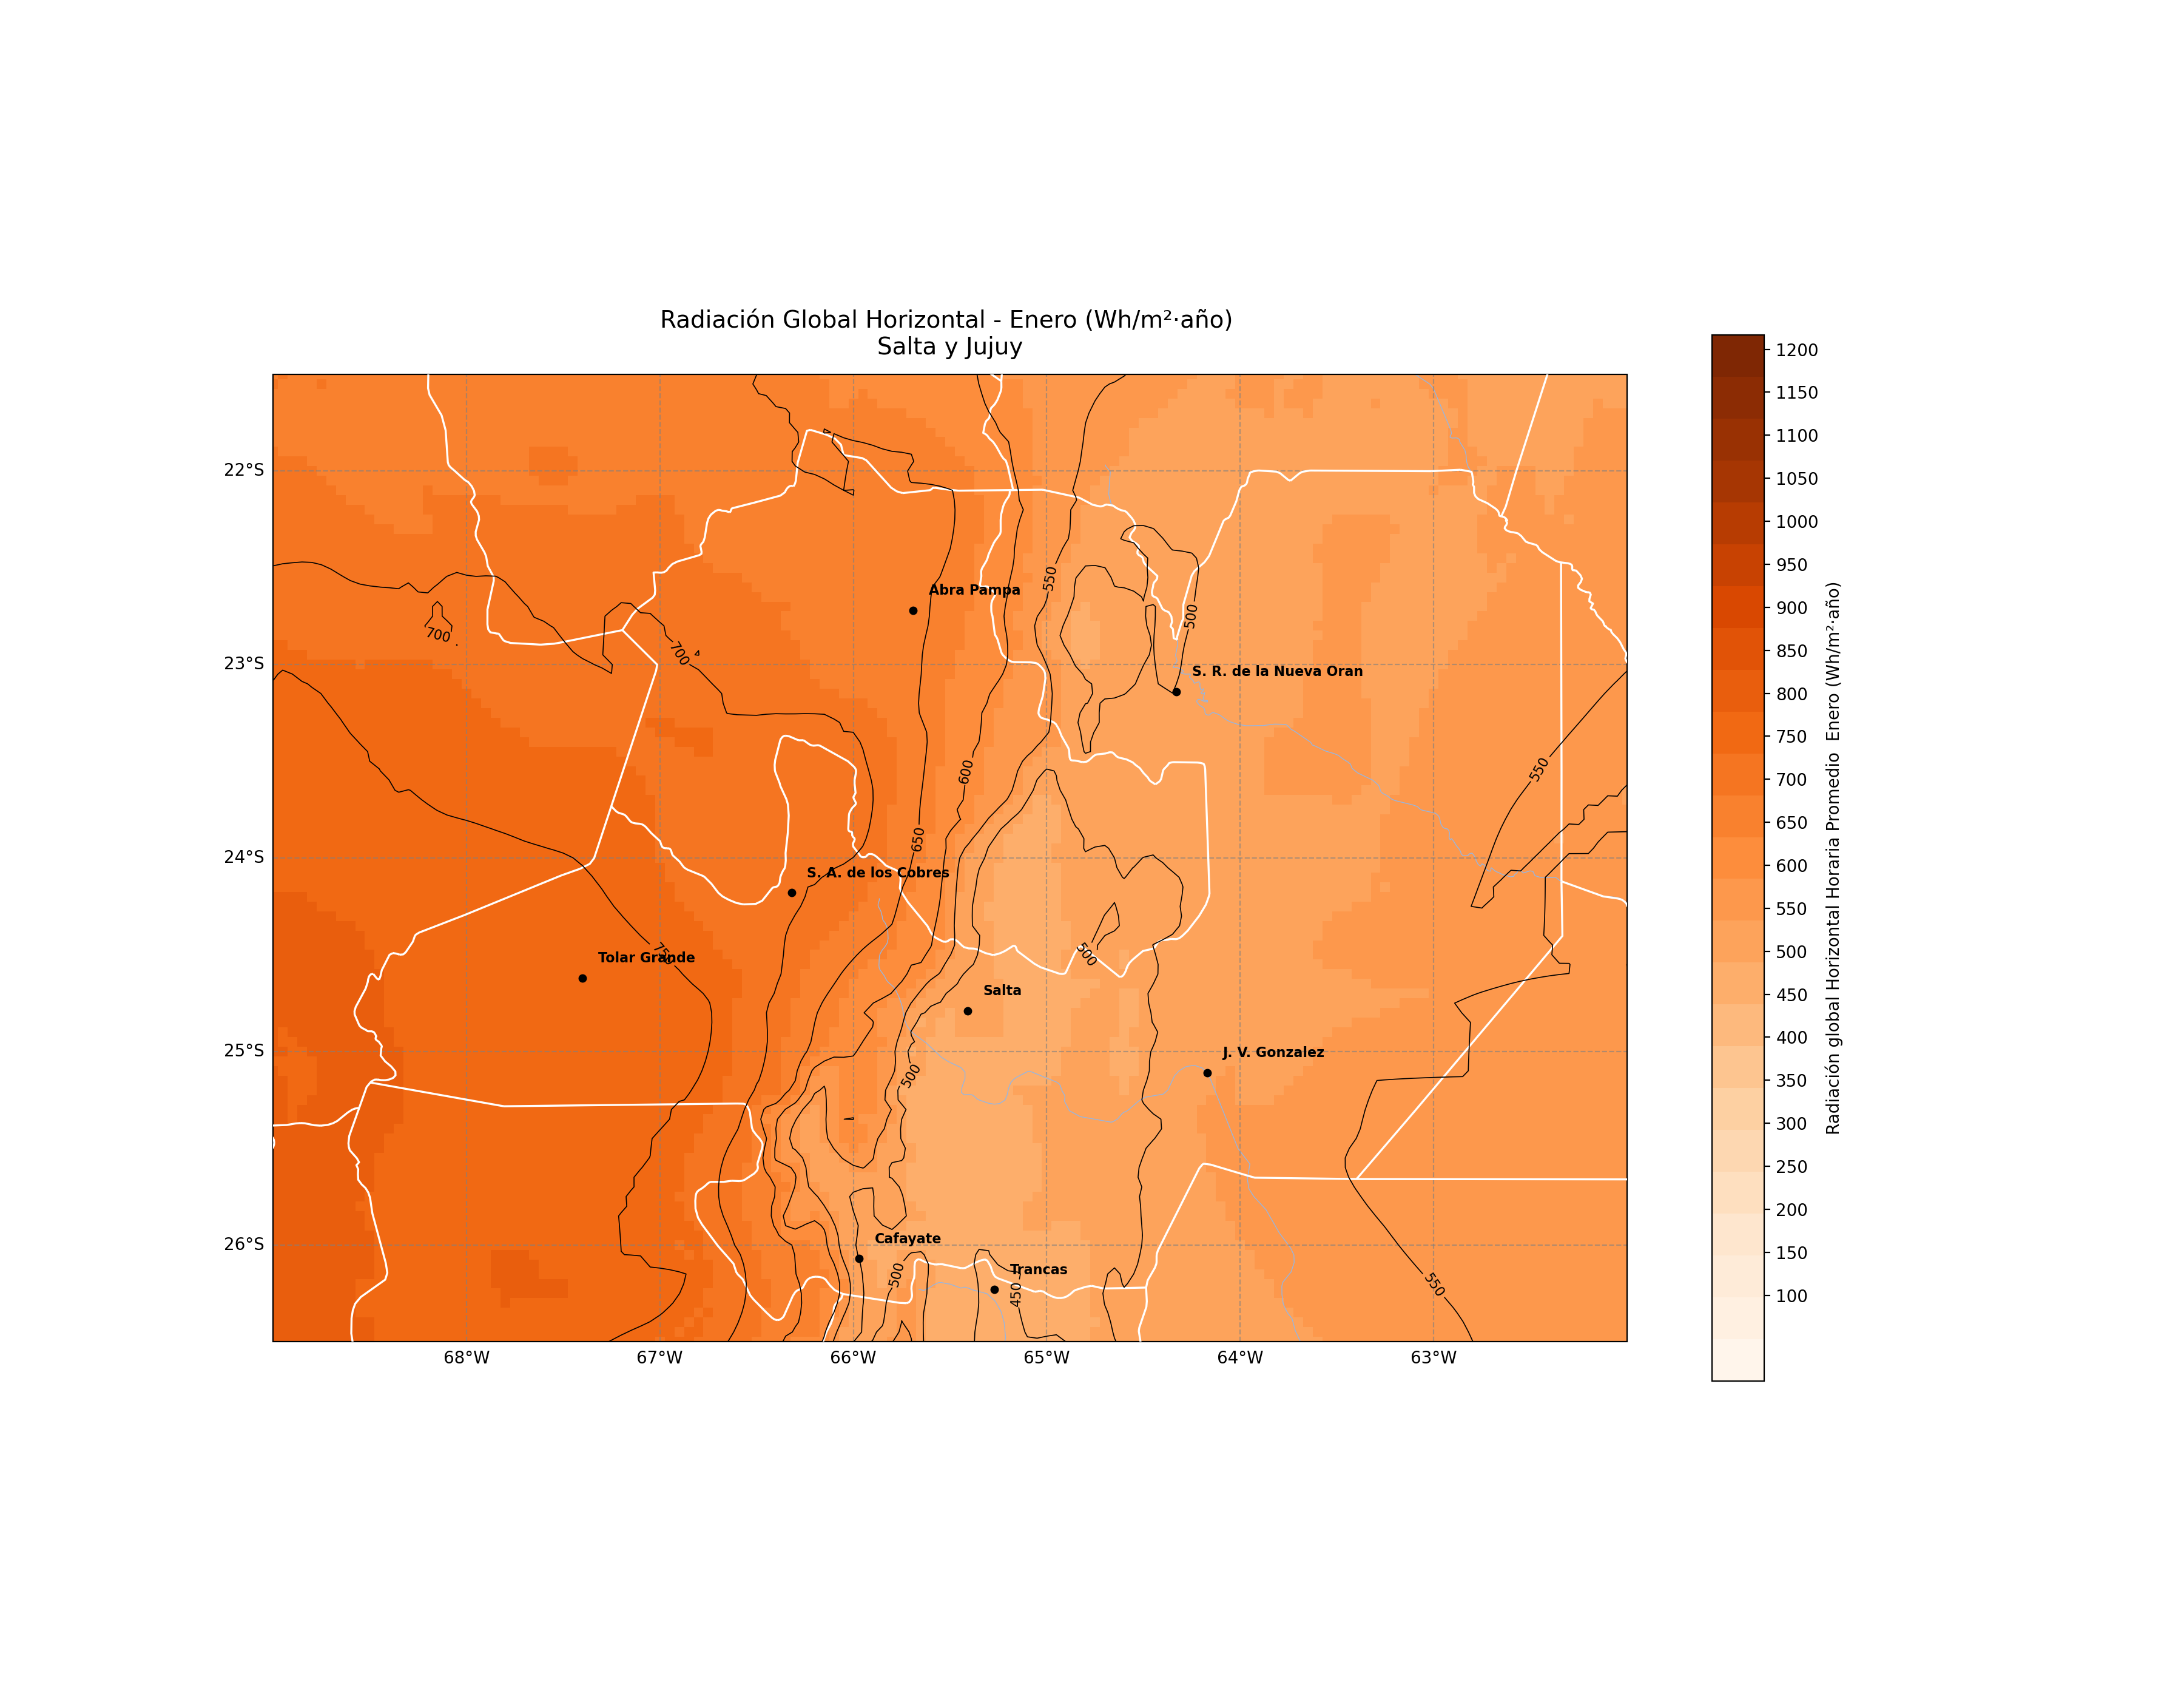
\includegraphics[width=0.99\textwidth]{figuras/Mapas/1_Enero.png}
%DIFDELCMD < %%%
%DIFDELCMD < \caption{%
{%DIFAUXCMD
\DIFdelFL{Mapa de GHI medio mensual – Enero (TMY).}}
%DIFAUXCMD
%DIFDELCMD < \end{figure}
%DIFDELCMD < 

%DIFDELCMD < \begin{figure}[H]
%DIFDELCMD < \centering
%DIFDELCMD < 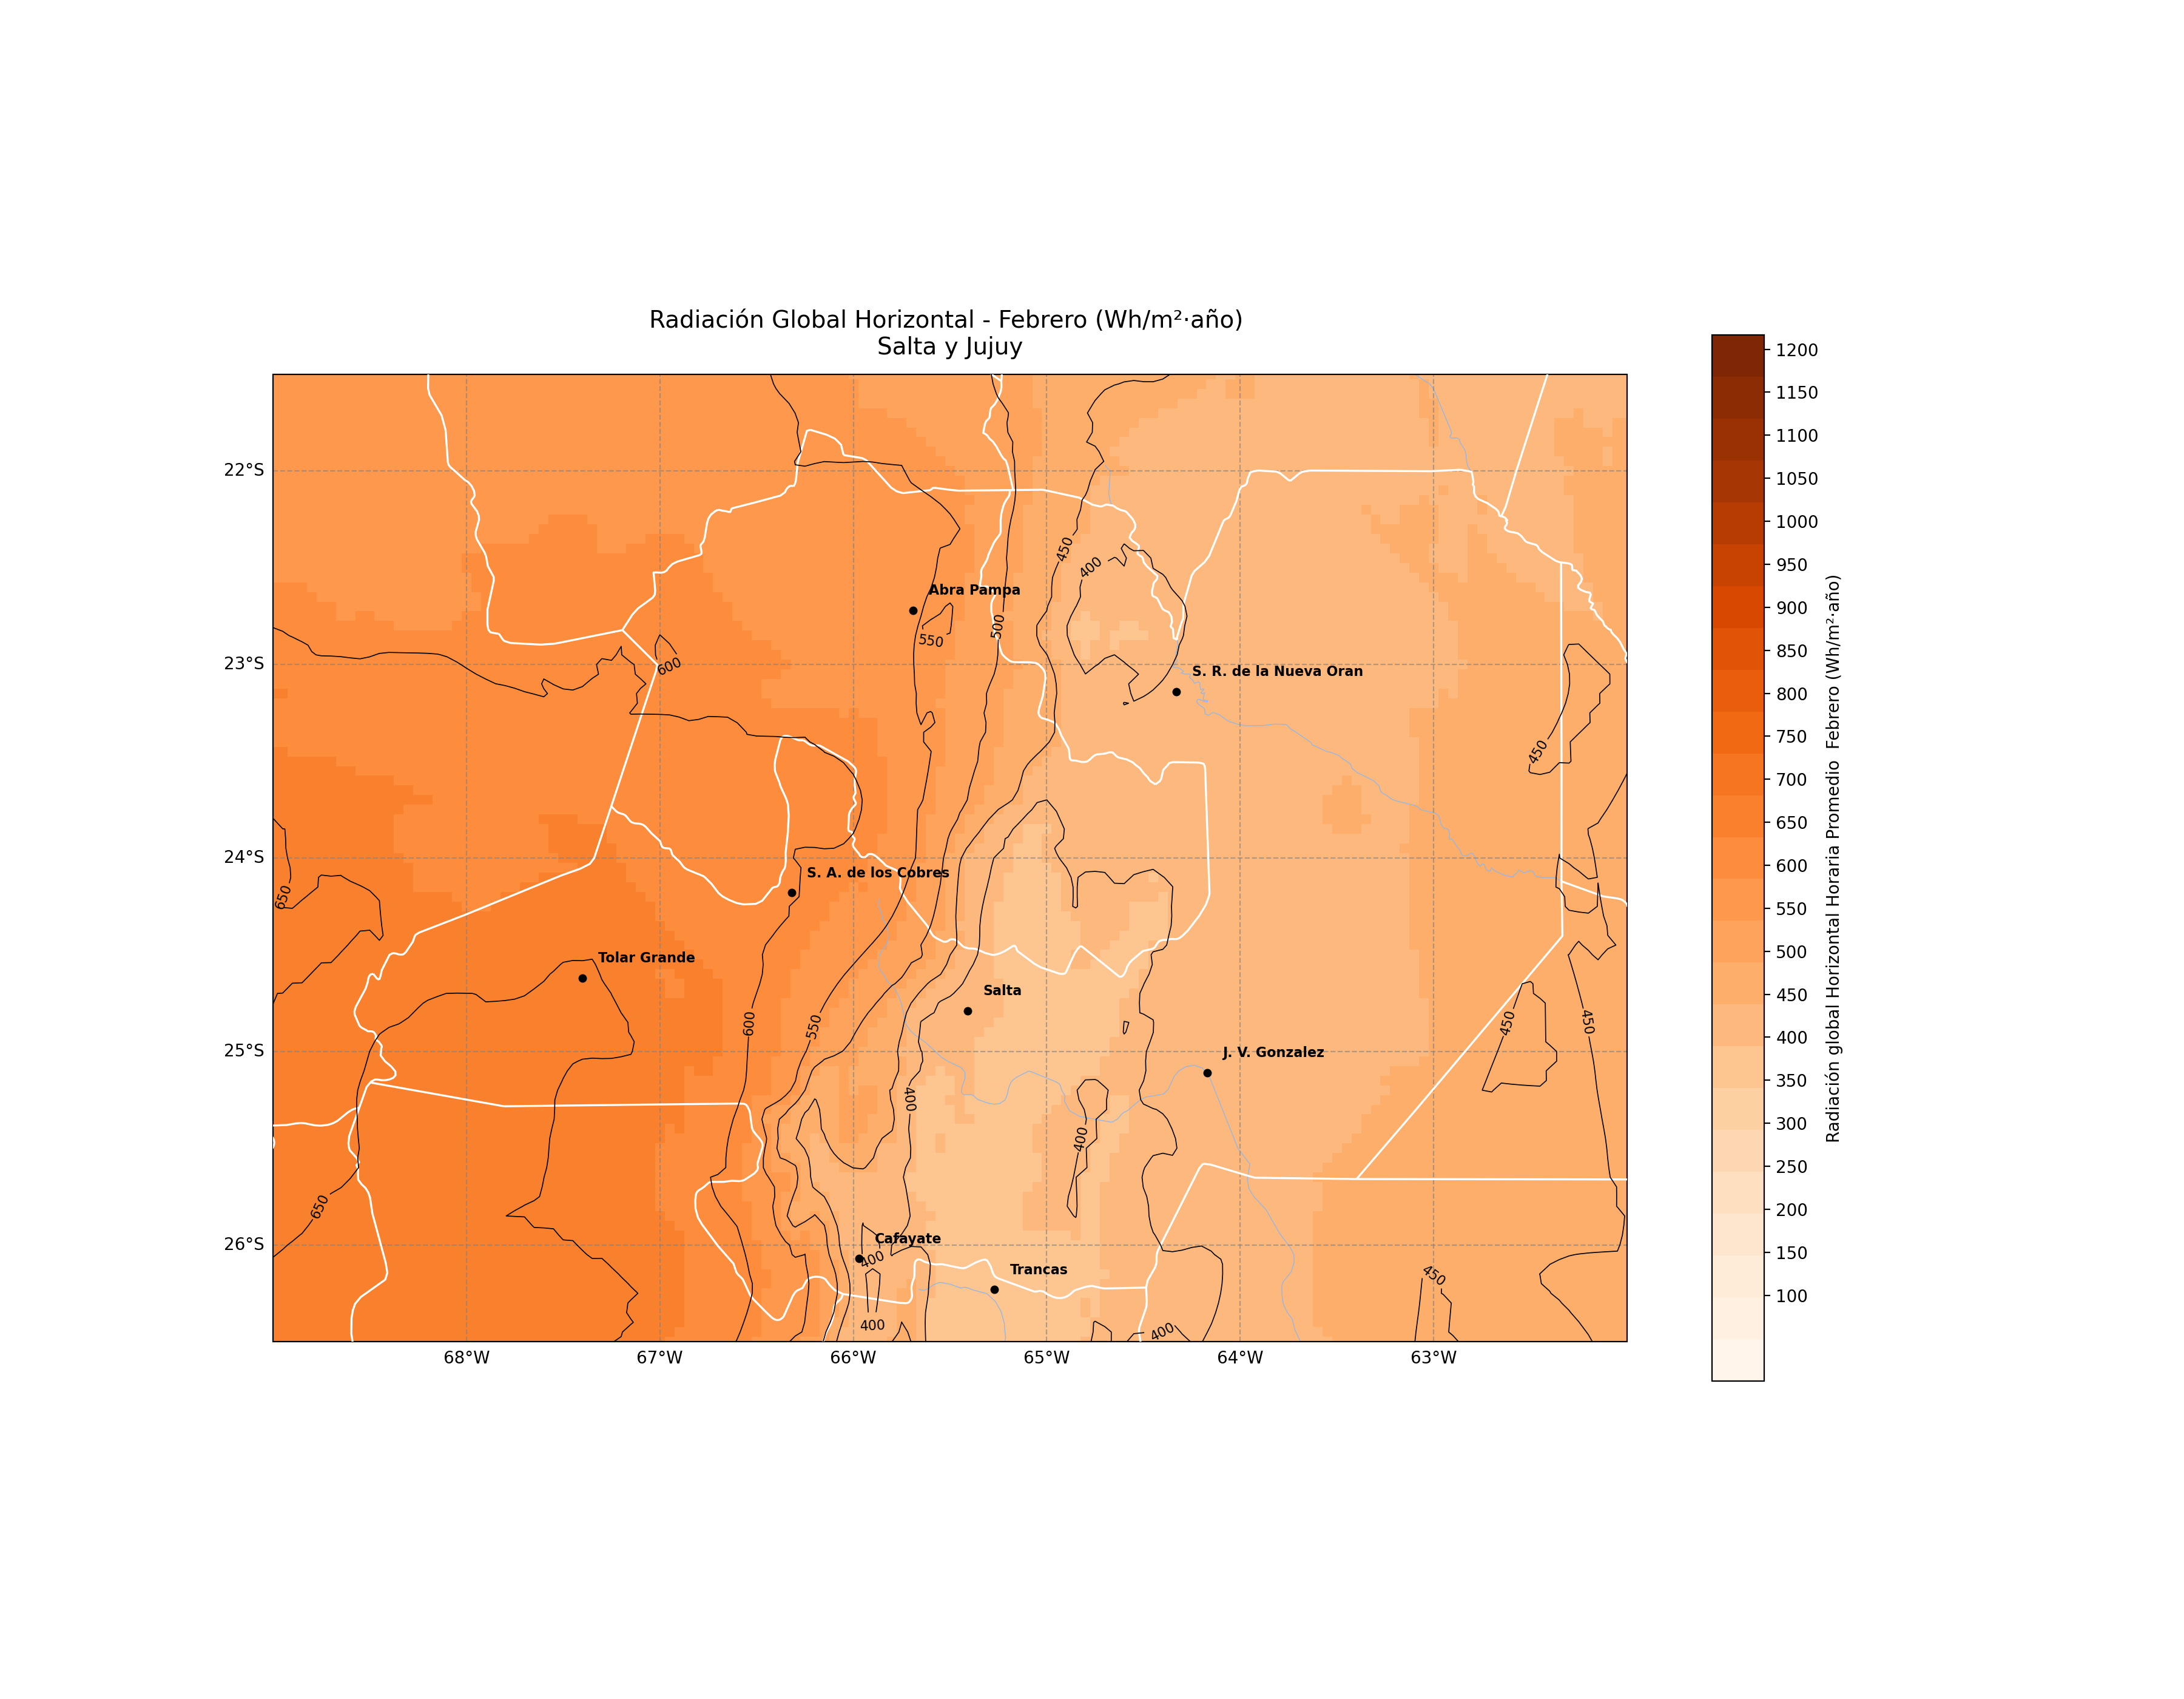
\includegraphics[width=0.9\textwidth]{figuras/Mapas/2_Febrero.png}
%DIFDELCMD < %%%
%DIFDELCMD < \caption{%
{%DIFAUXCMD
\DIFdelFL{Mapa de GHI medio mensual – Febrero (TMY).}}
%DIFAUXCMD
%DIFDELCMD < \end{figure}
%DIFDELCMD < 

%DIFDELCMD < \begin{figure}[H]
%DIFDELCMD < \centering
%DIFDELCMD < 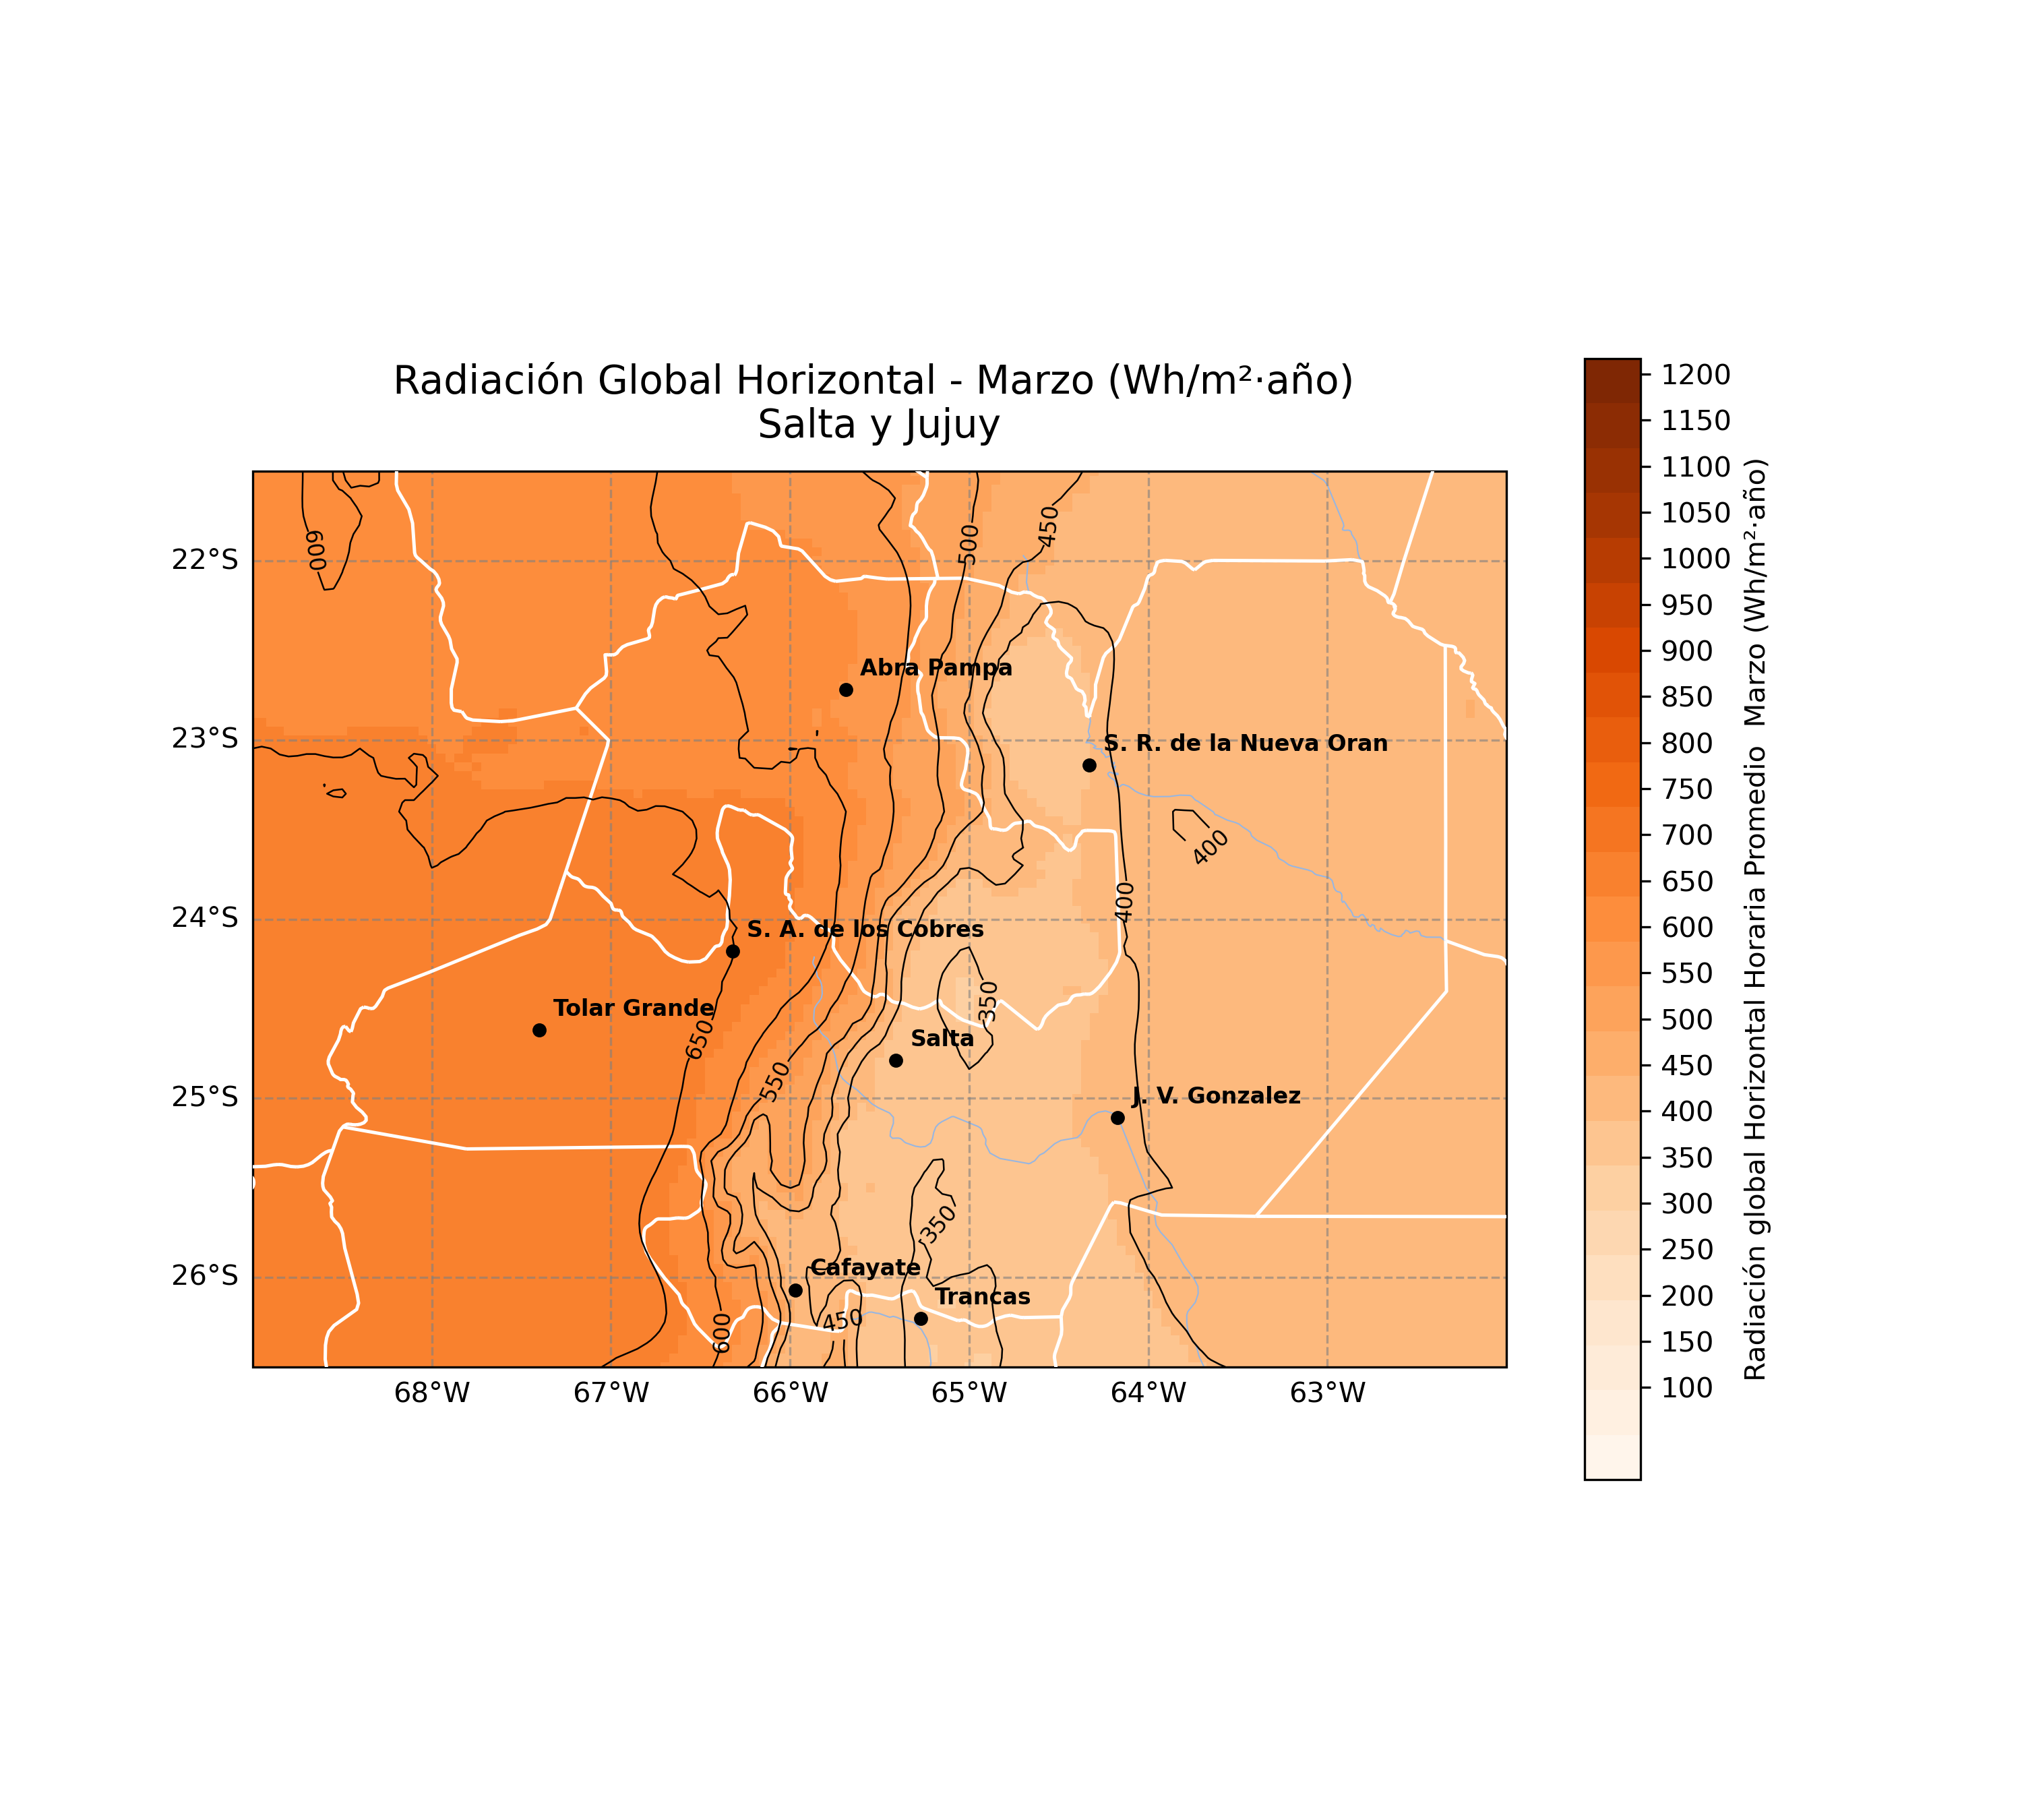
\includegraphics[width=0.99\textwidth]{figuras/Mapas/3_Marzo.png}
%DIFDELCMD < %%%
%DIFDELCMD < \caption{%
{%DIFAUXCMD
\DIFdelFL{Mapa de GHI medio mensual – Marzo (TMY).}}
%DIFAUXCMD
%DIFDELCMD < \end{figure}
%DIFDELCMD < 

%DIFDELCMD < \begin{figure}[H]
%DIFDELCMD < \centering
%DIFDELCMD < 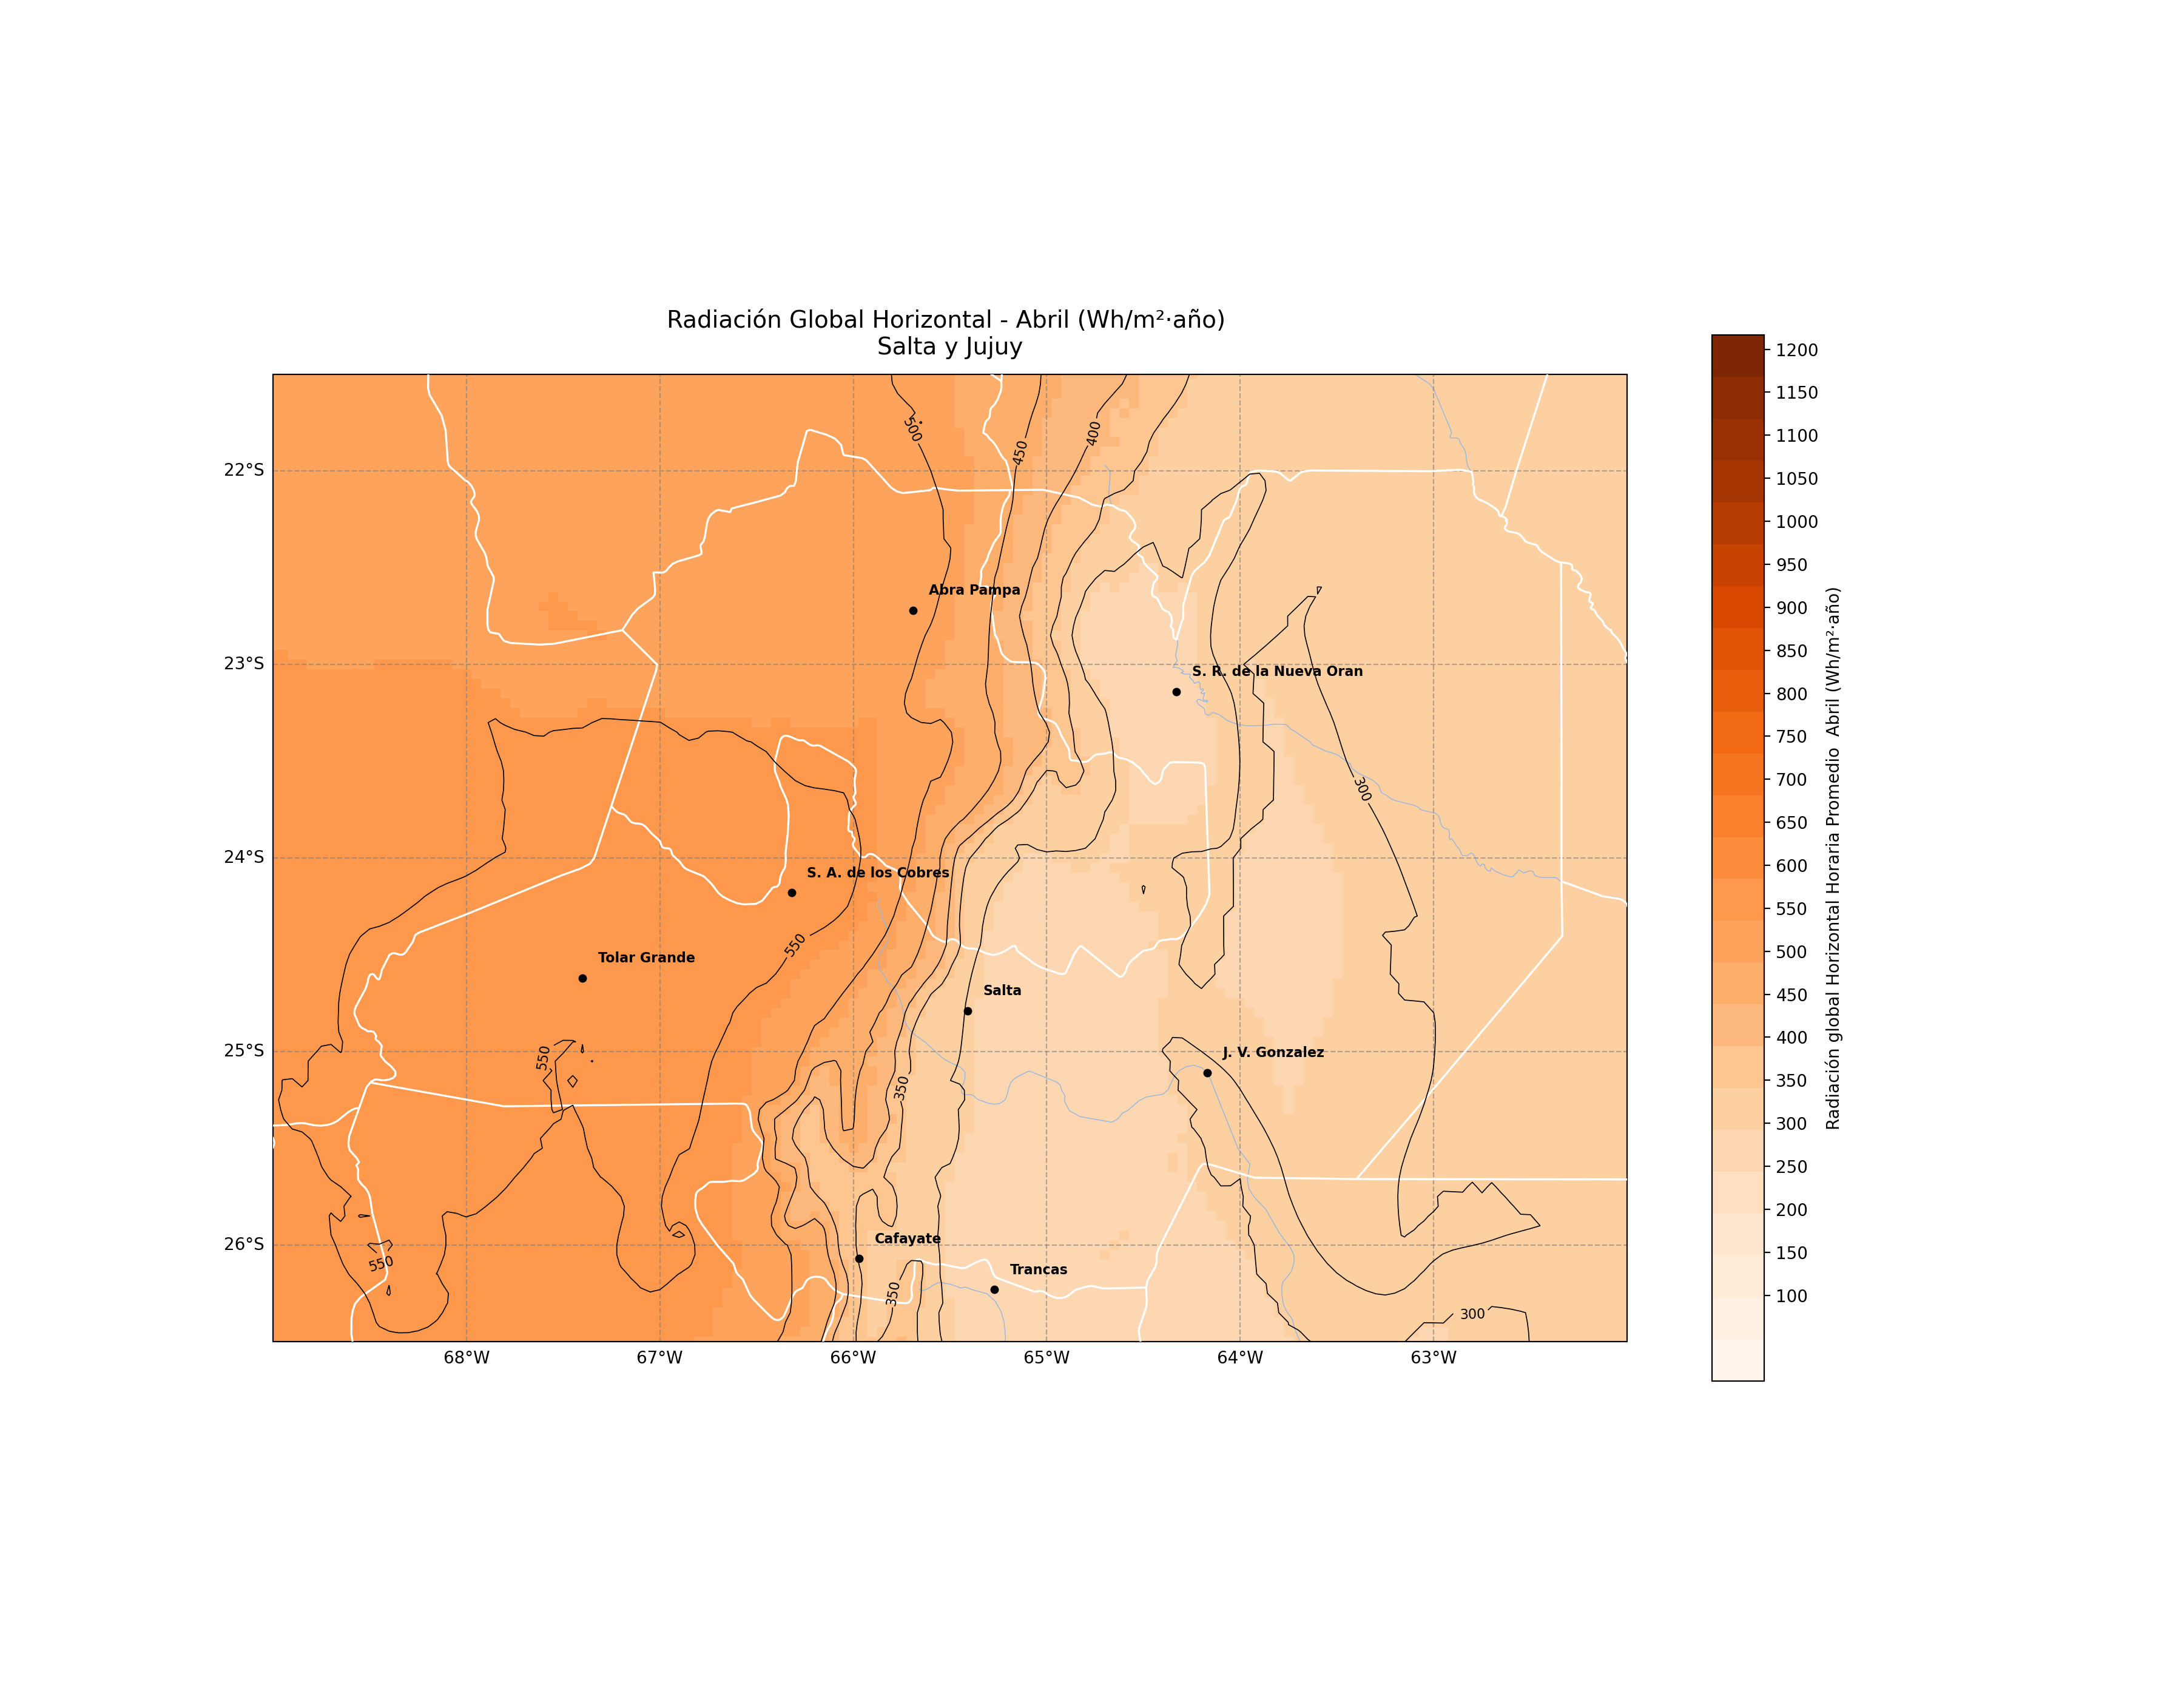
\includegraphics[width=0.99\textwidth]{figuras/Mapas/4_Abril.png}
%DIFDELCMD < %%%
%DIFDELCMD < \caption{%
{%DIFAUXCMD
\DIFdelFL{Mapa de GHI medio mensual – Abril (TMY).}}
%DIFAUXCMD
%DIFDELCMD < \end{figure}
%DIFDELCMD < 

%DIFDELCMD < \begin{figure}[H]
%DIFDELCMD < \centering
%DIFDELCMD < 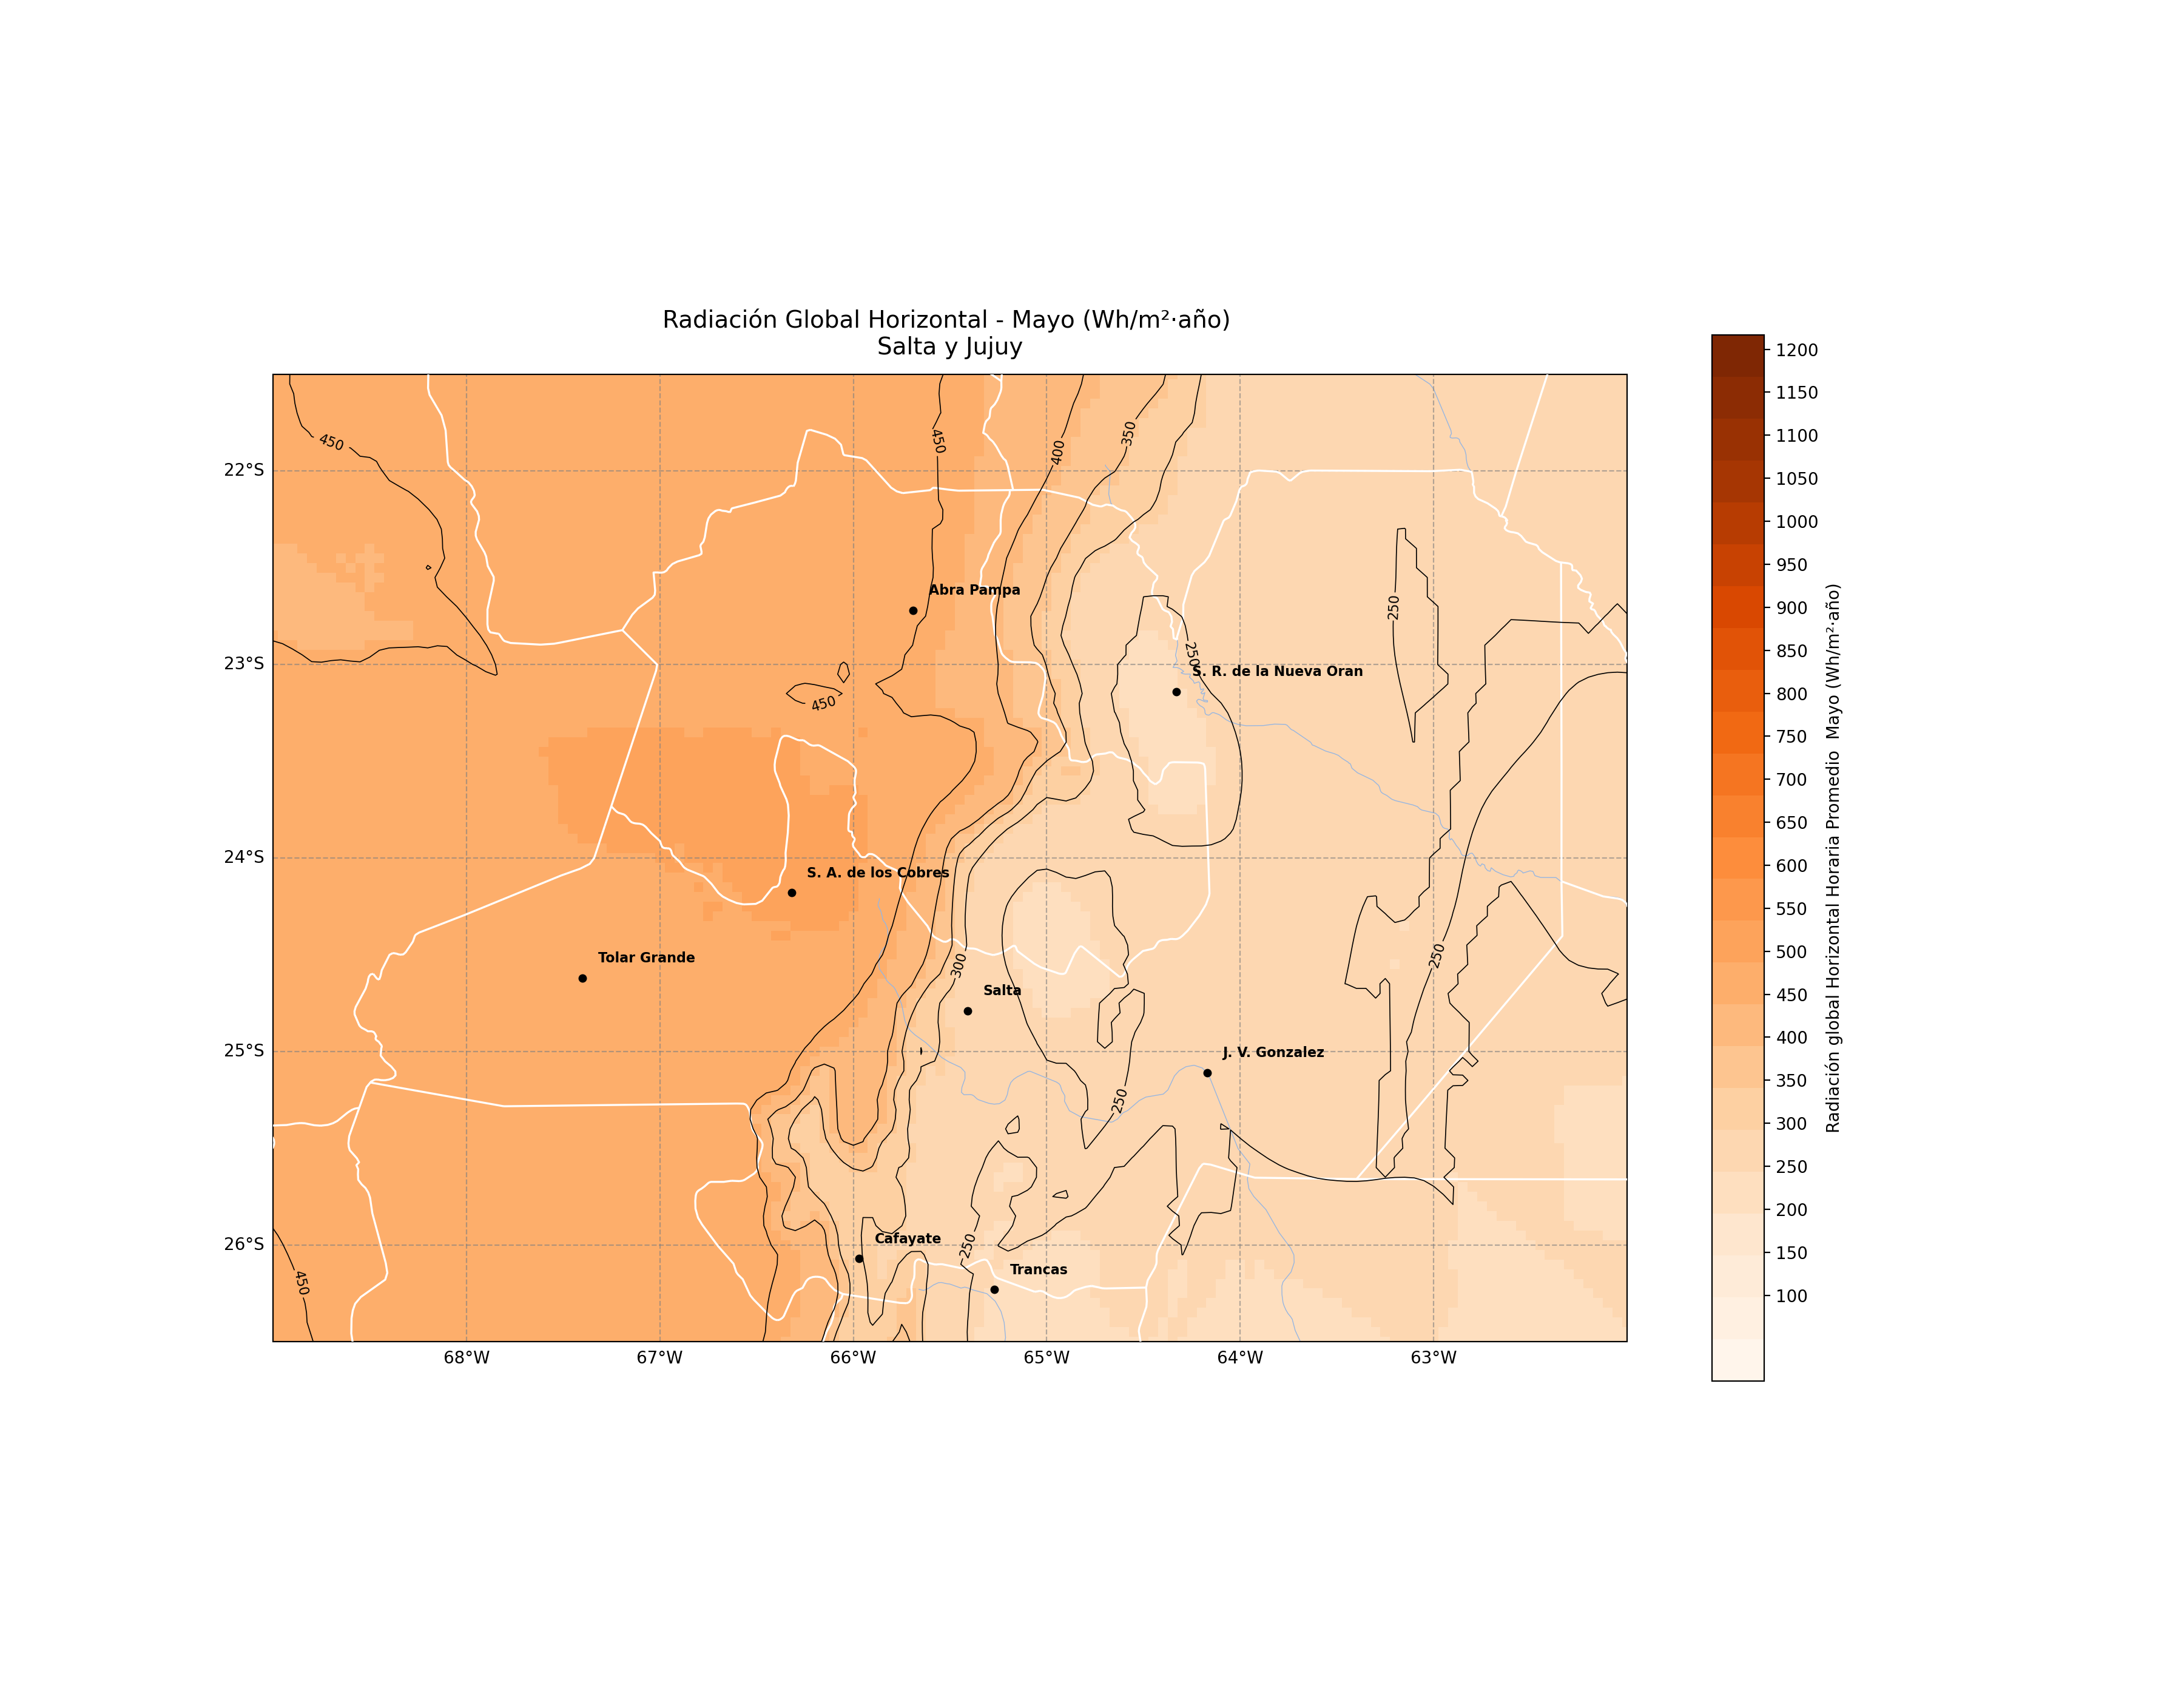
\includegraphics[width=0.99\textwidth]{figuras/Mapas/5_Mayo.png}
%DIFDELCMD < %%%
%DIFDELCMD < \caption{%
{%DIFAUXCMD
\DIFdelFL{Mapa de GHI medio mensual – Mayo (TMY).}}
%DIFAUXCMD
%DIFDELCMD < \end{figure}
%DIFDELCMD < 

%DIFDELCMD < \begin{figure}[H]
%DIFDELCMD < \centering
%DIFDELCMD < 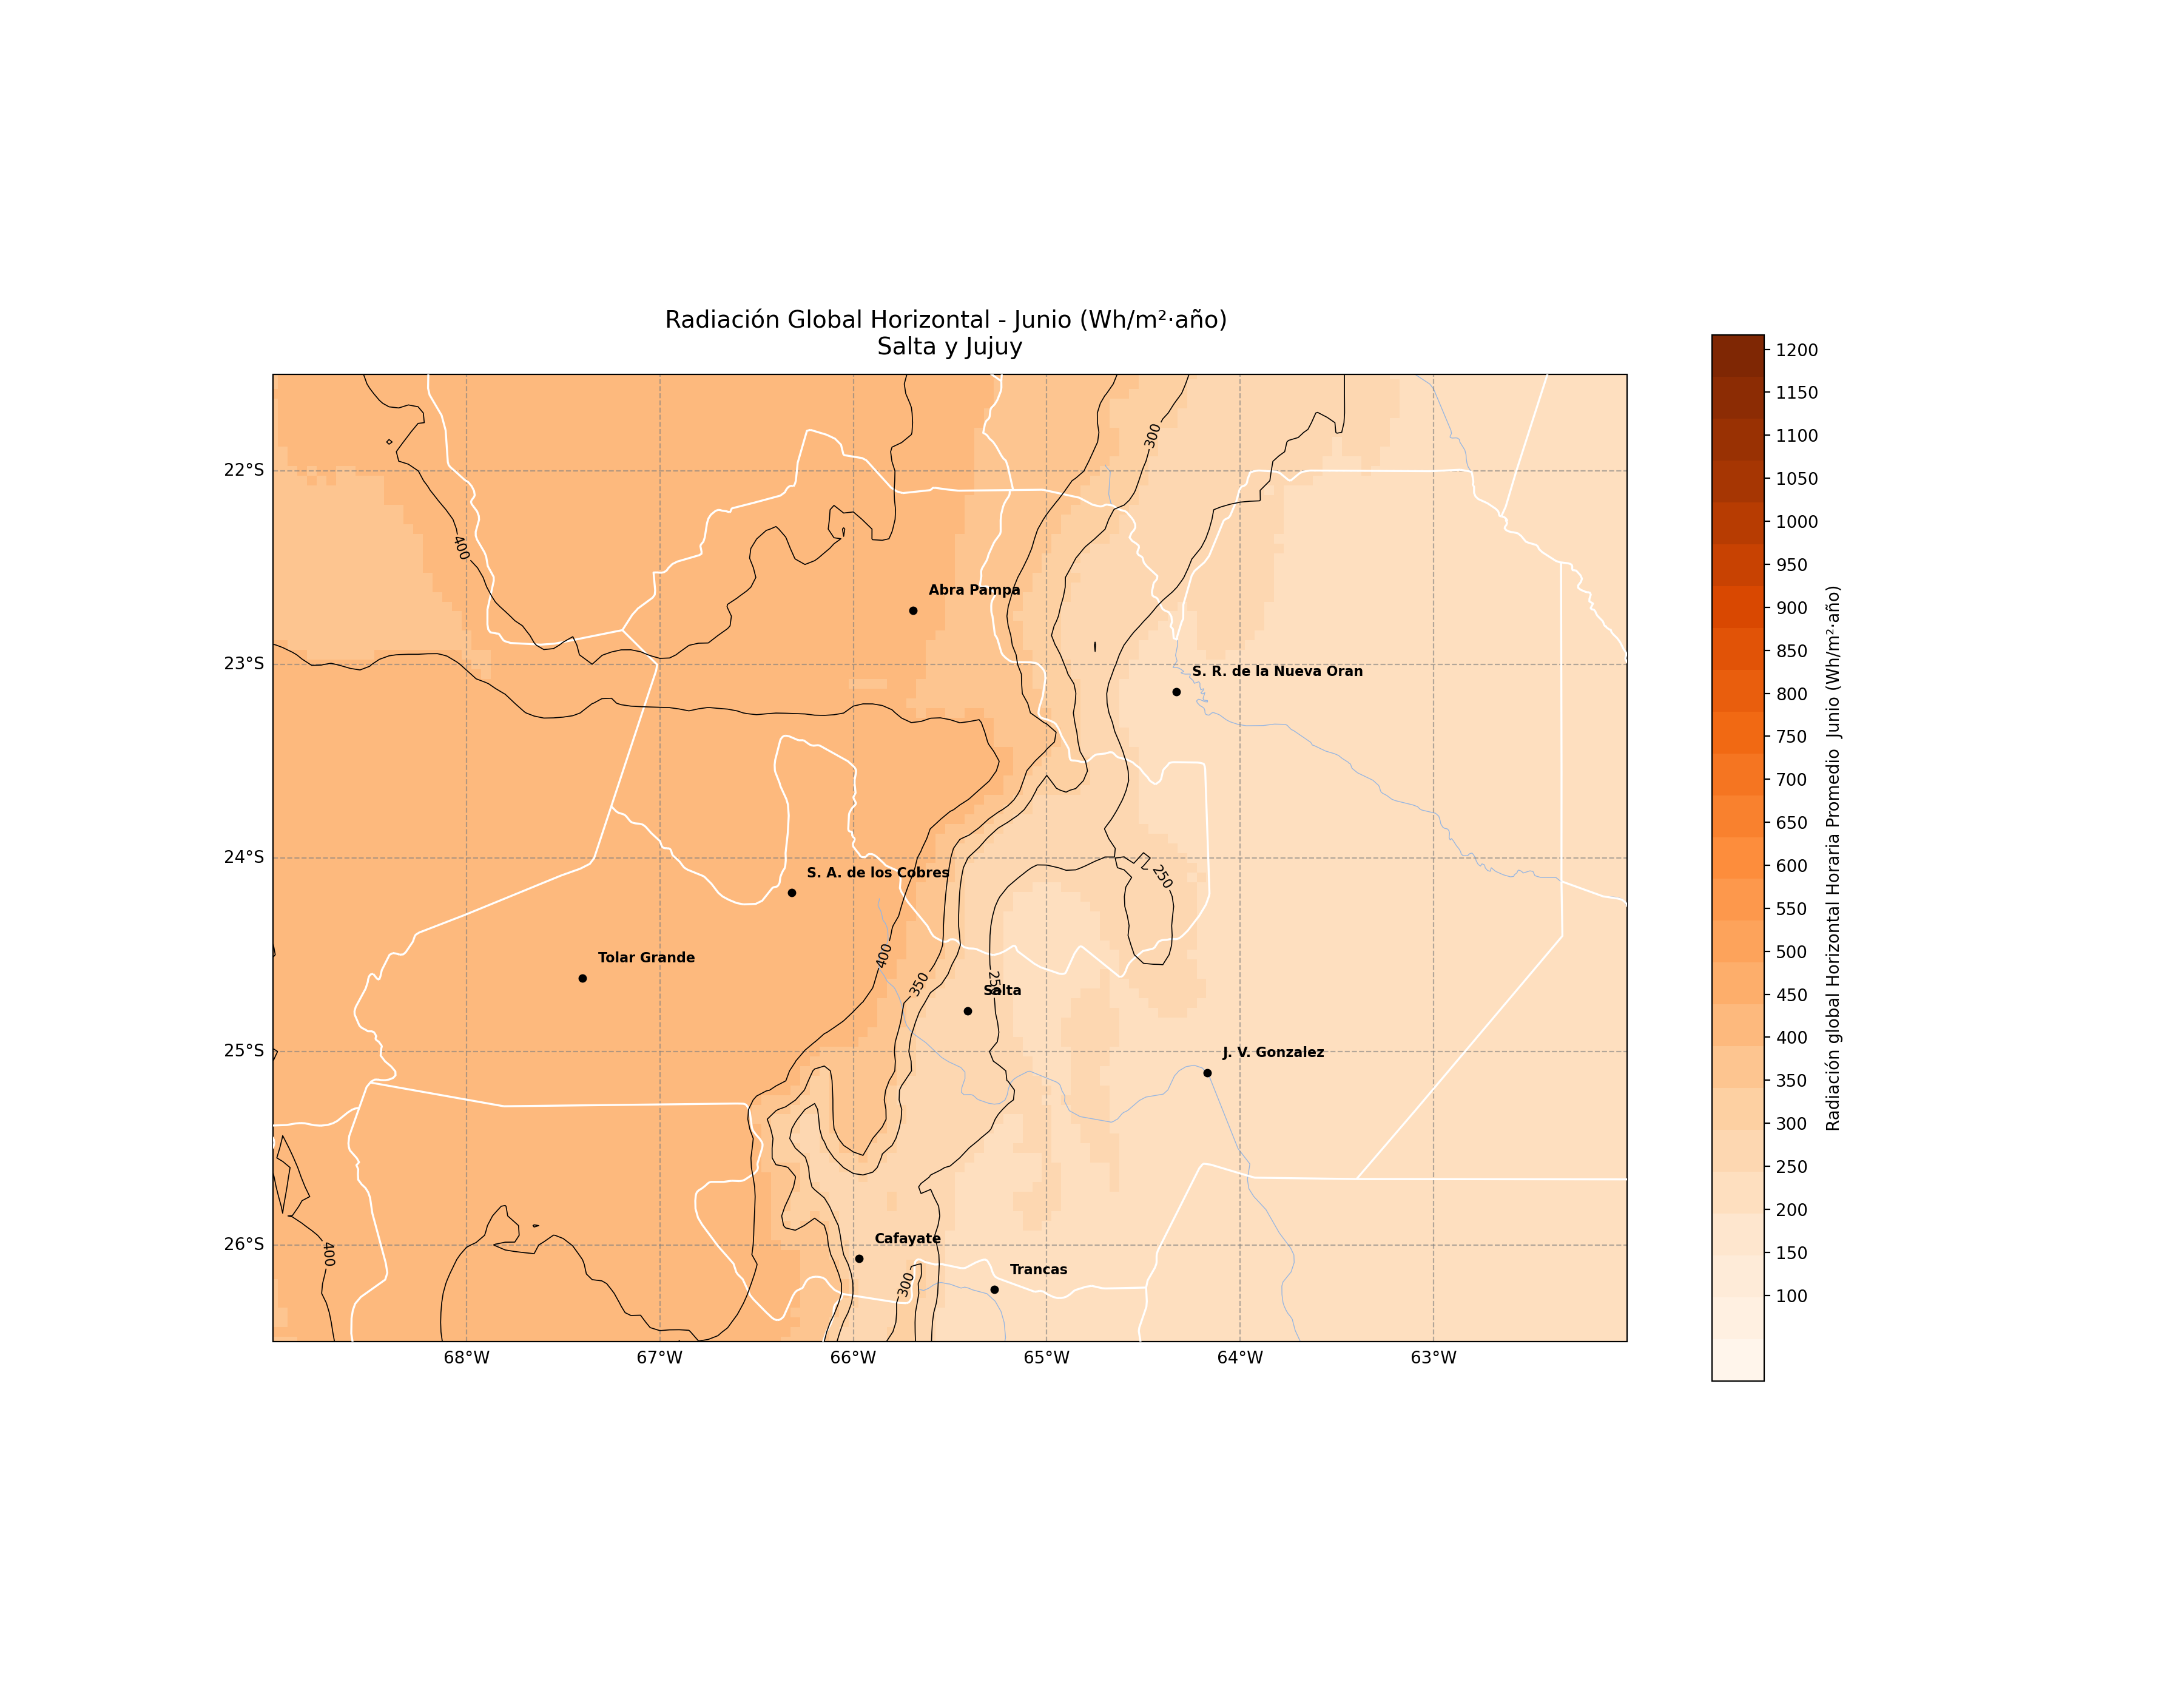
\includegraphics[width=0.99\textwidth]{figuras/Mapas/6_Junio.png}
%DIFDELCMD < %%%
%DIFDELCMD < \caption{%
{%DIFAUXCMD
\DIFdelFL{Mapa de GHI medio mensual – Junio (TMY).}}
%DIFAUXCMD
%DIFDELCMD < \end{figure}
%DIFDELCMD < 

%DIFDELCMD < \begin{figure}[H]
%DIFDELCMD < \centering
%DIFDELCMD < 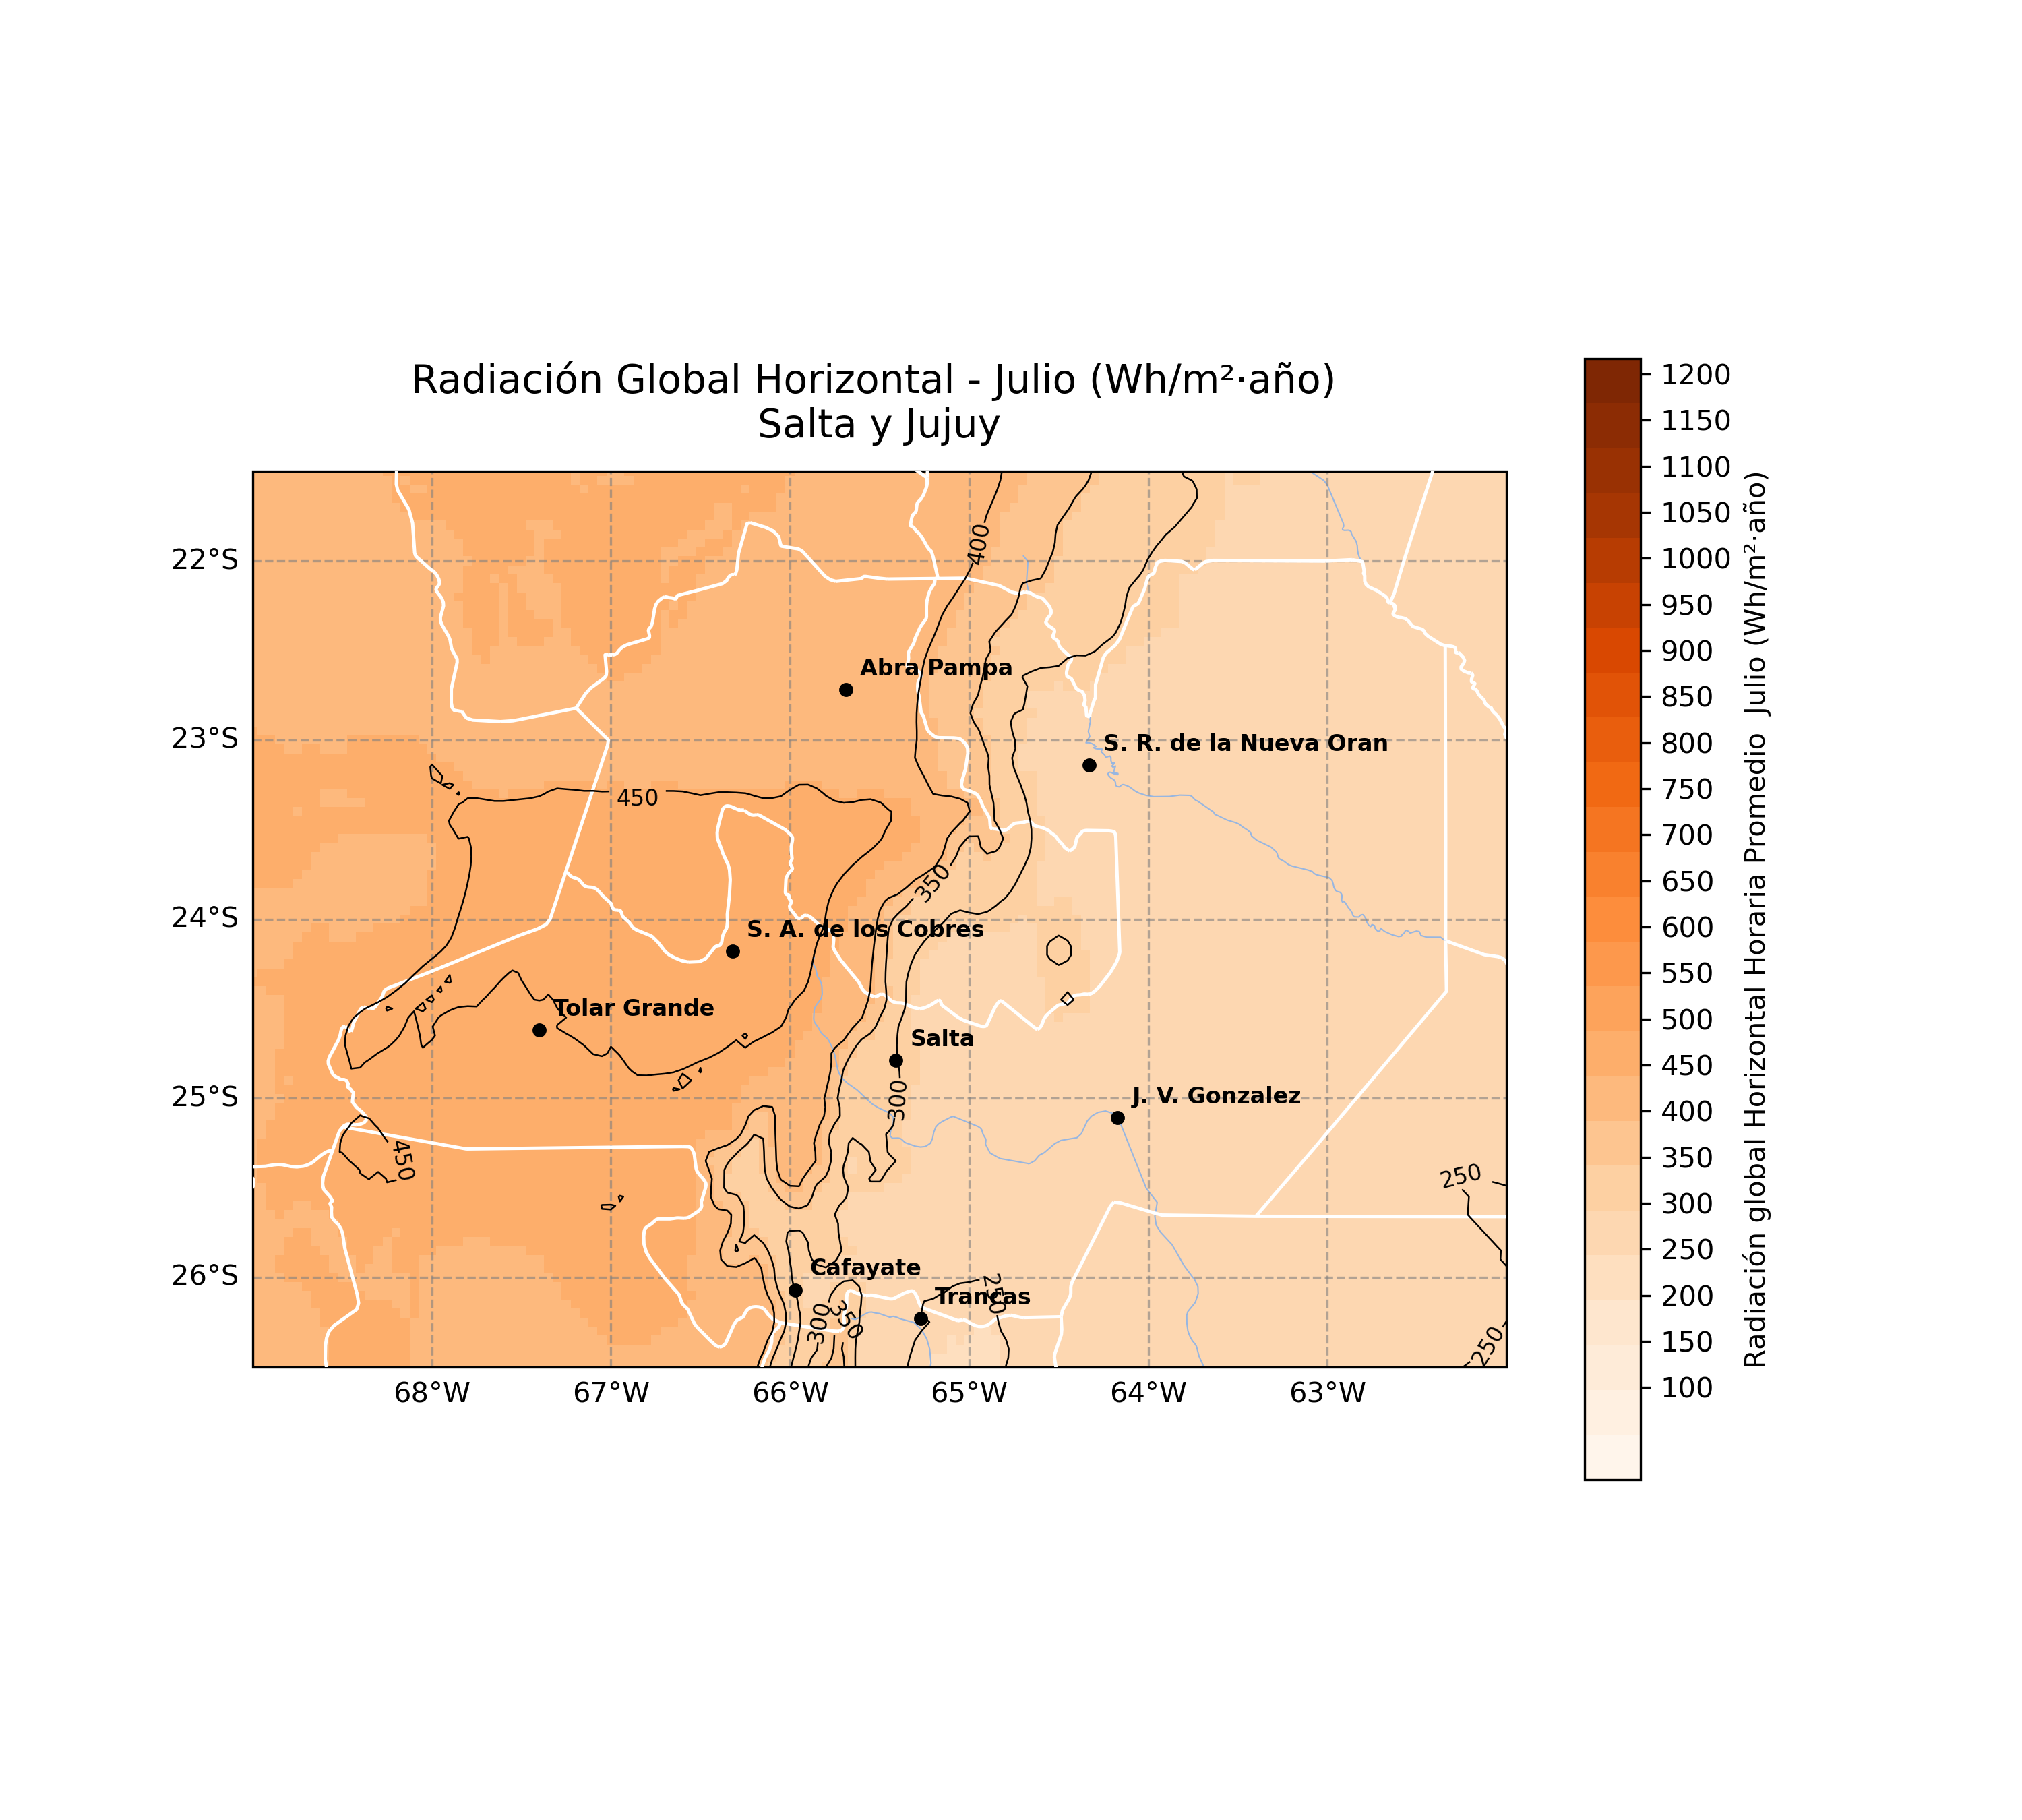
\includegraphics[width=0.99\textwidth]{figuras/Mapas/7_Julio.png}
%DIFDELCMD < %%%
%DIFDELCMD < \caption{%
{%DIFAUXCMD
\DIFdelFL{Mapa de GHI medio mensual – Julio (TMY).}}
%DIFAUXCMD
%DIFDELCMD < \end{figure}
%DIFDELCMD < 

%DIFDELCMD < \begin{figure}[H]
%DIFDELCMD < \centering
%DIFDELCMD < 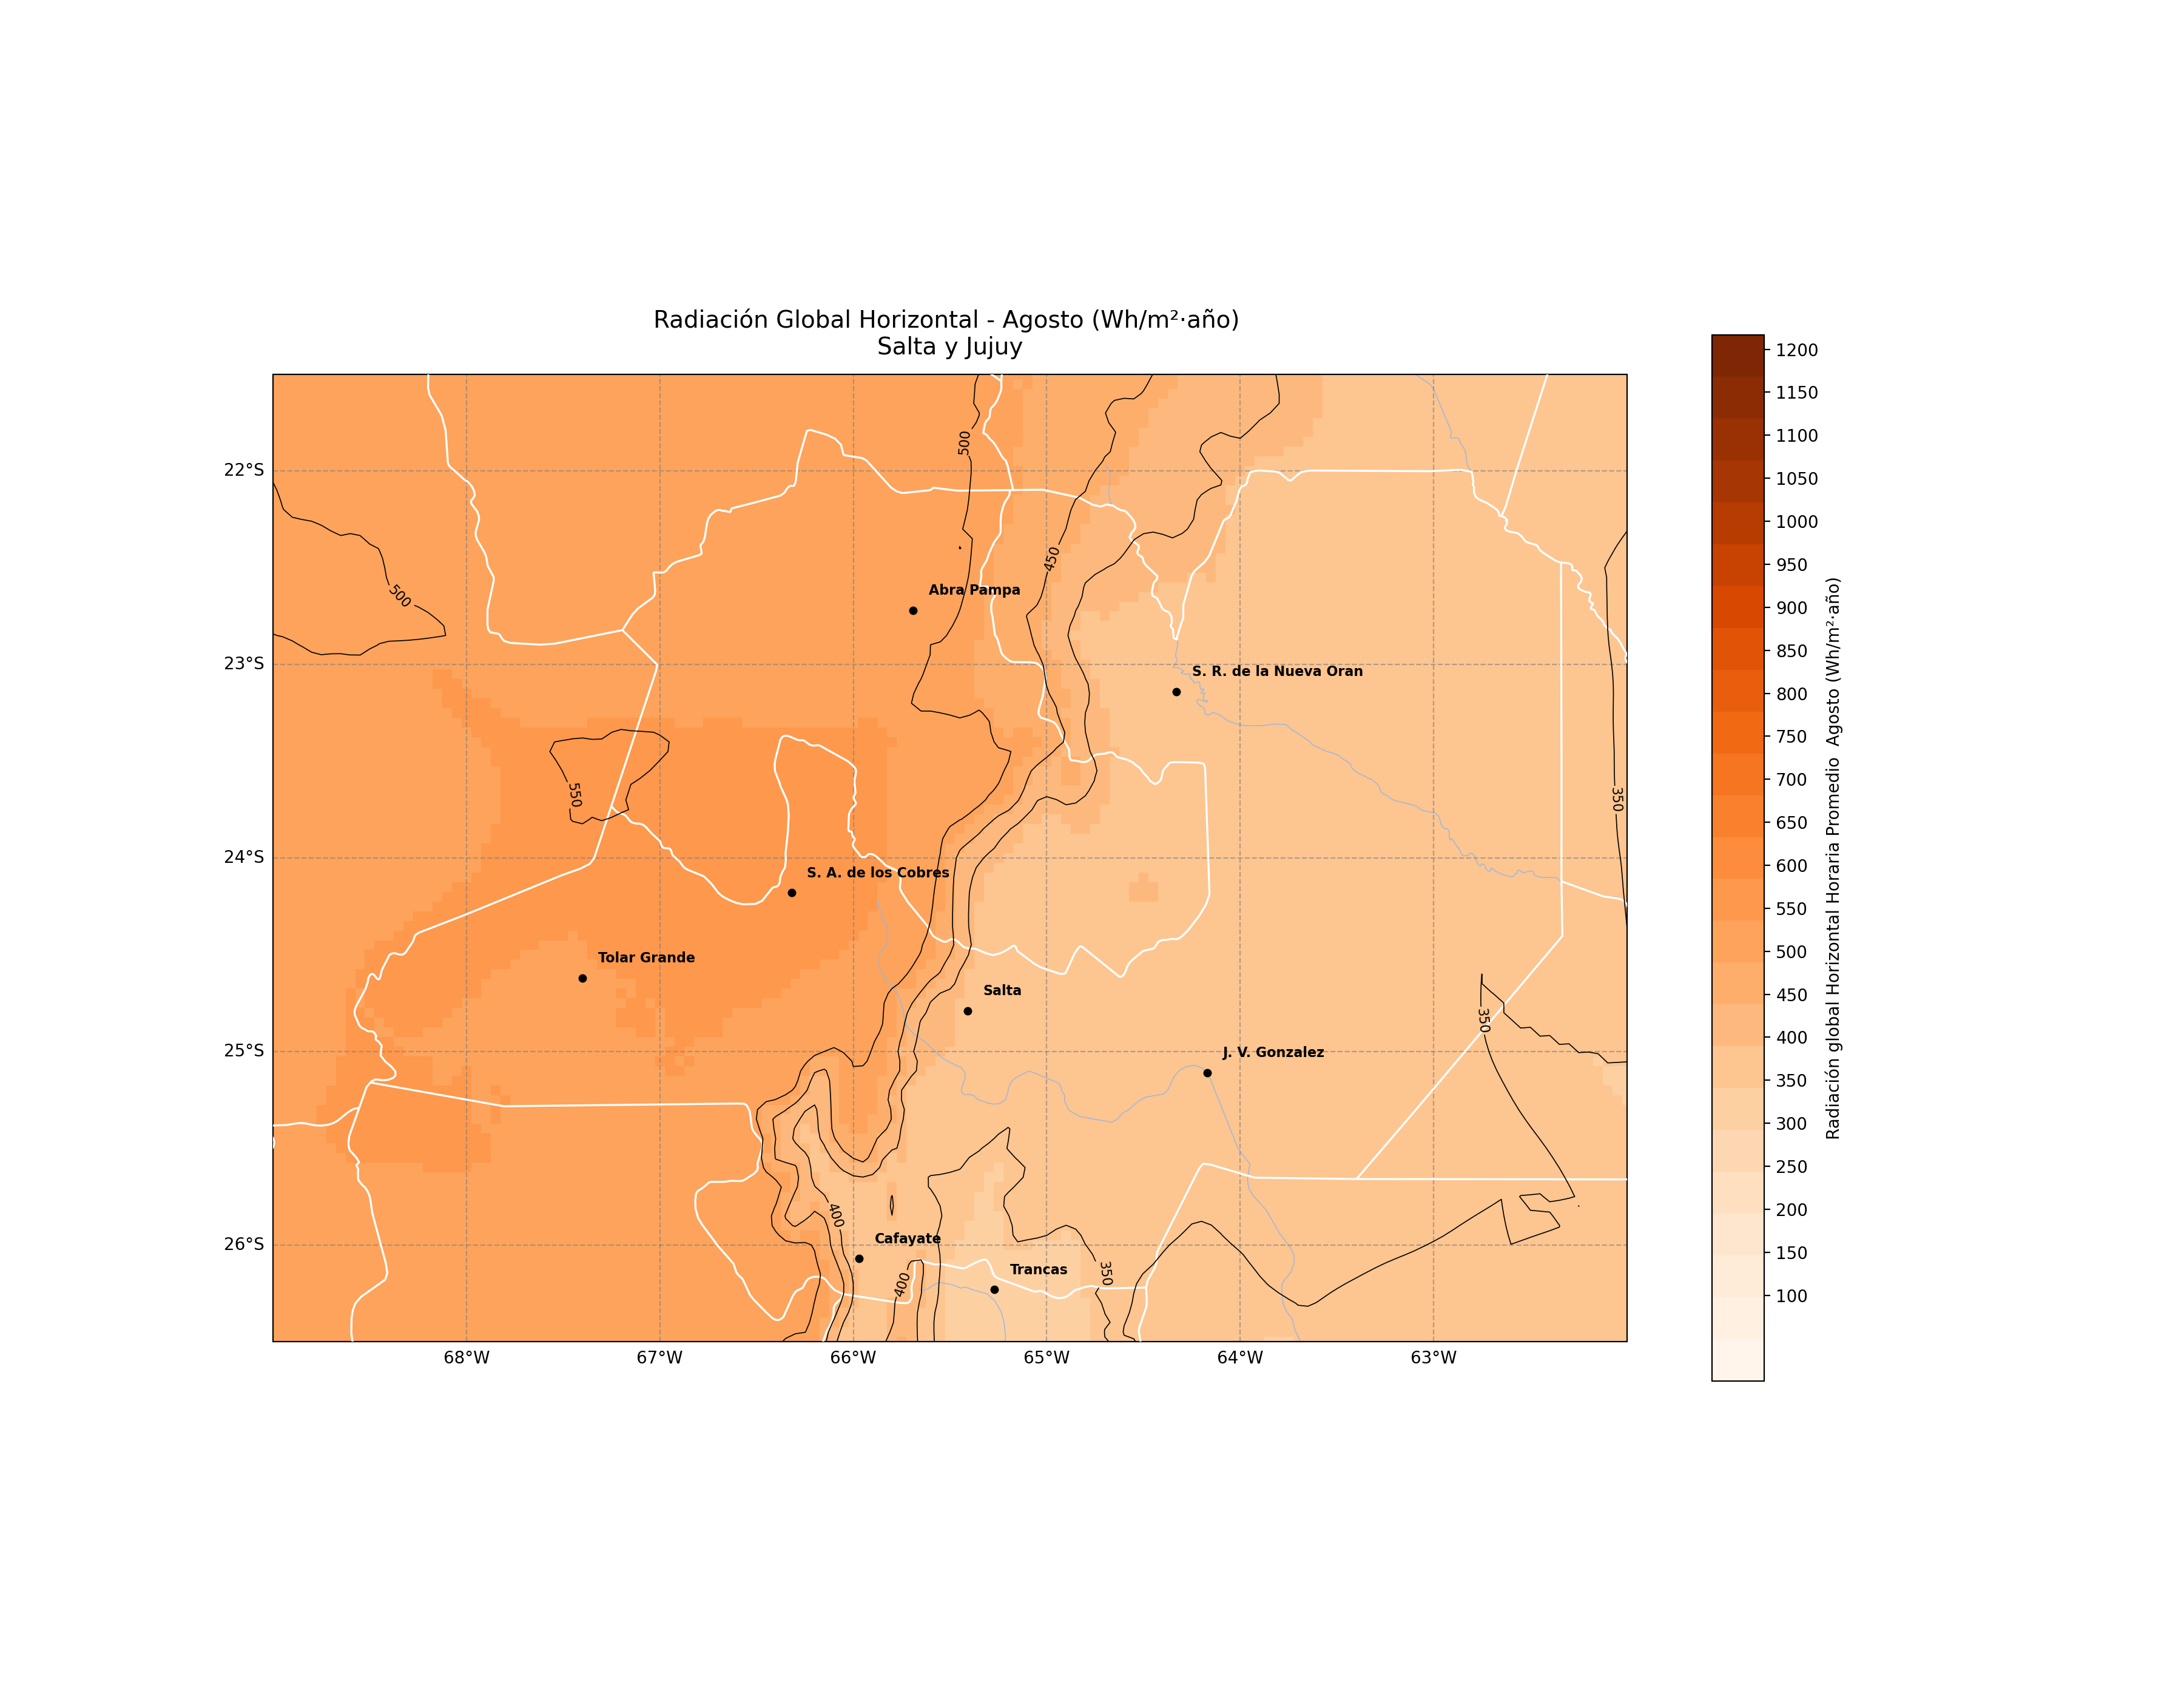
\includegraphics[width=0.99\textwidth]{figuras/Mapas/8_Agosto.png}
%DIFDELCMD < %%%
%DIFDELCMD < \caption{%
{%DIFAUXCMD
\DIFdelFL{Mapa de GHI medio mensual – Agosto (TMY).}}
%DIFAUXCMD
%DIFDELCMD < \end{figure}
%DIFDELCMD < 

%DIFDELCMD < \begin{figure}[H]
%DIFDELCMD < \centering
%DIFDELCMD < 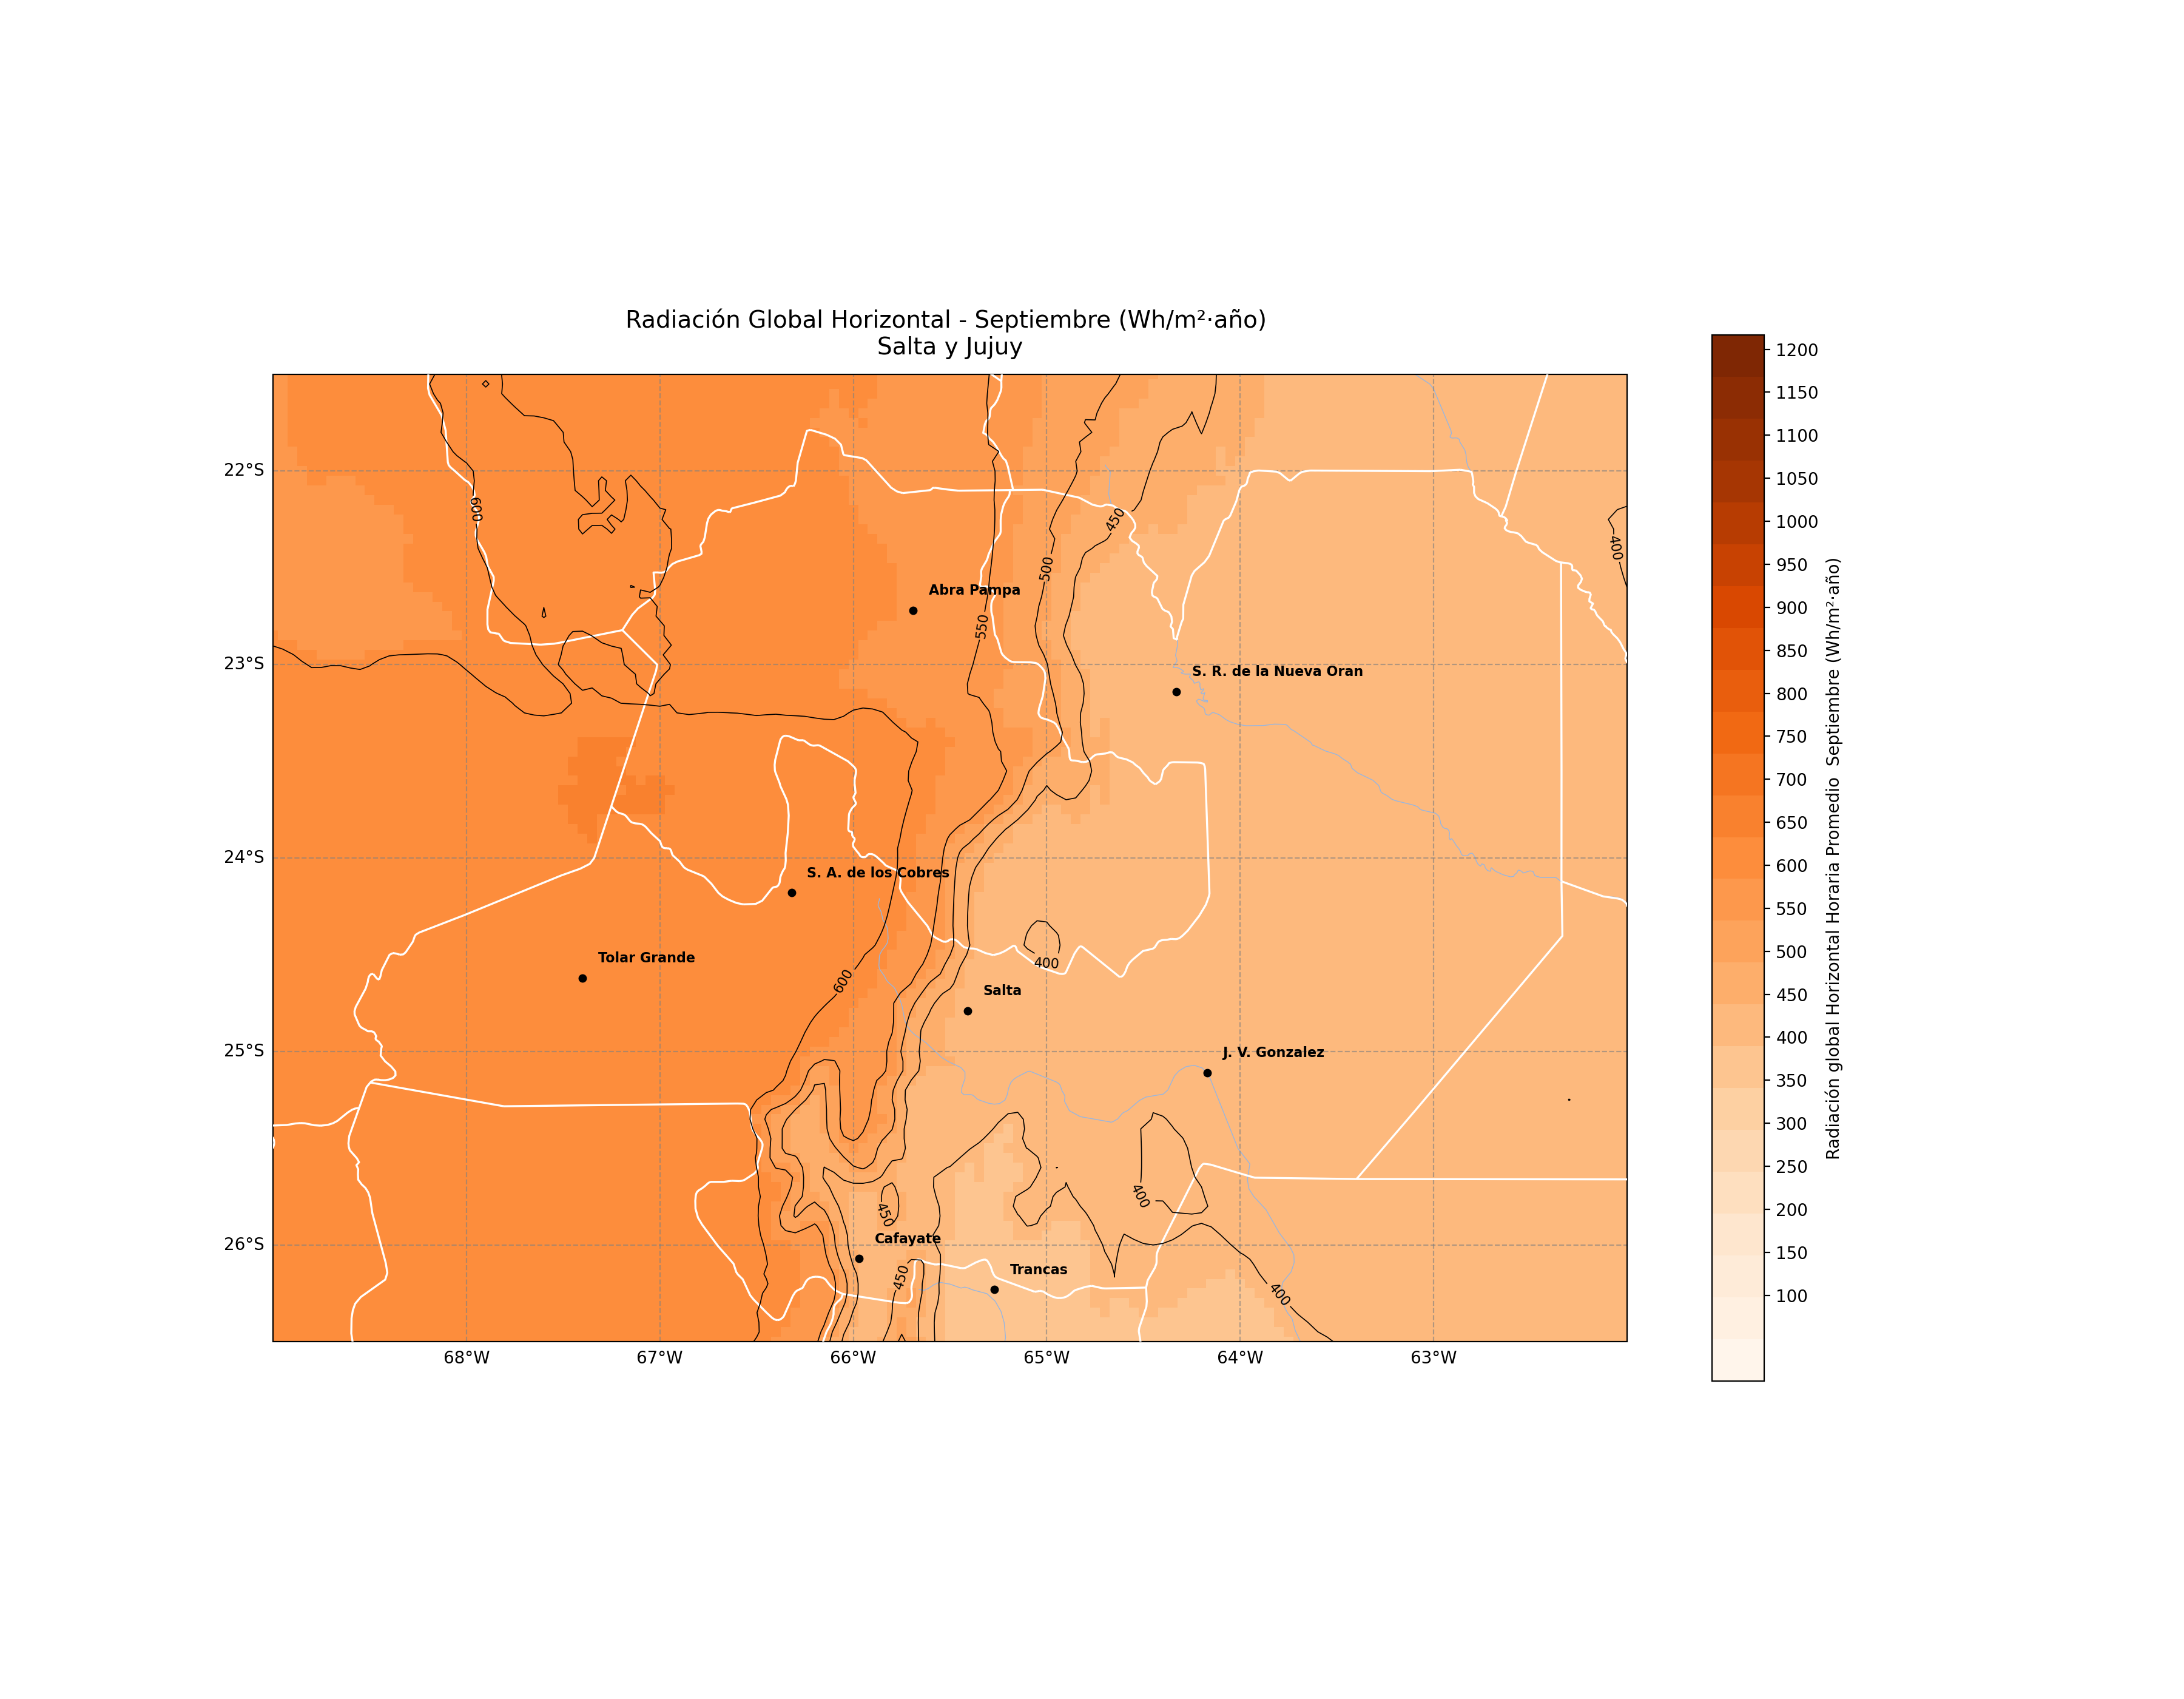
\includegraphics[width=0.99\textwidth]{figuras/Mapas/9_Septiembre.png}
%DIFDELCMD < %%%
%DIFDELCMD < \caption{%
{%DIFAUXCMD
\DIFdelFL{Mapa de GHI medio mensual – Septiembre (TMY).}}
%DIFAUXCMD
%DIFDELCMD < \end{figure}
%DIFDELCMD < 

%DIFDELCMD < \begin{figure}[H]
%DIFDELCMD < \centering
%DIFDELCMD < 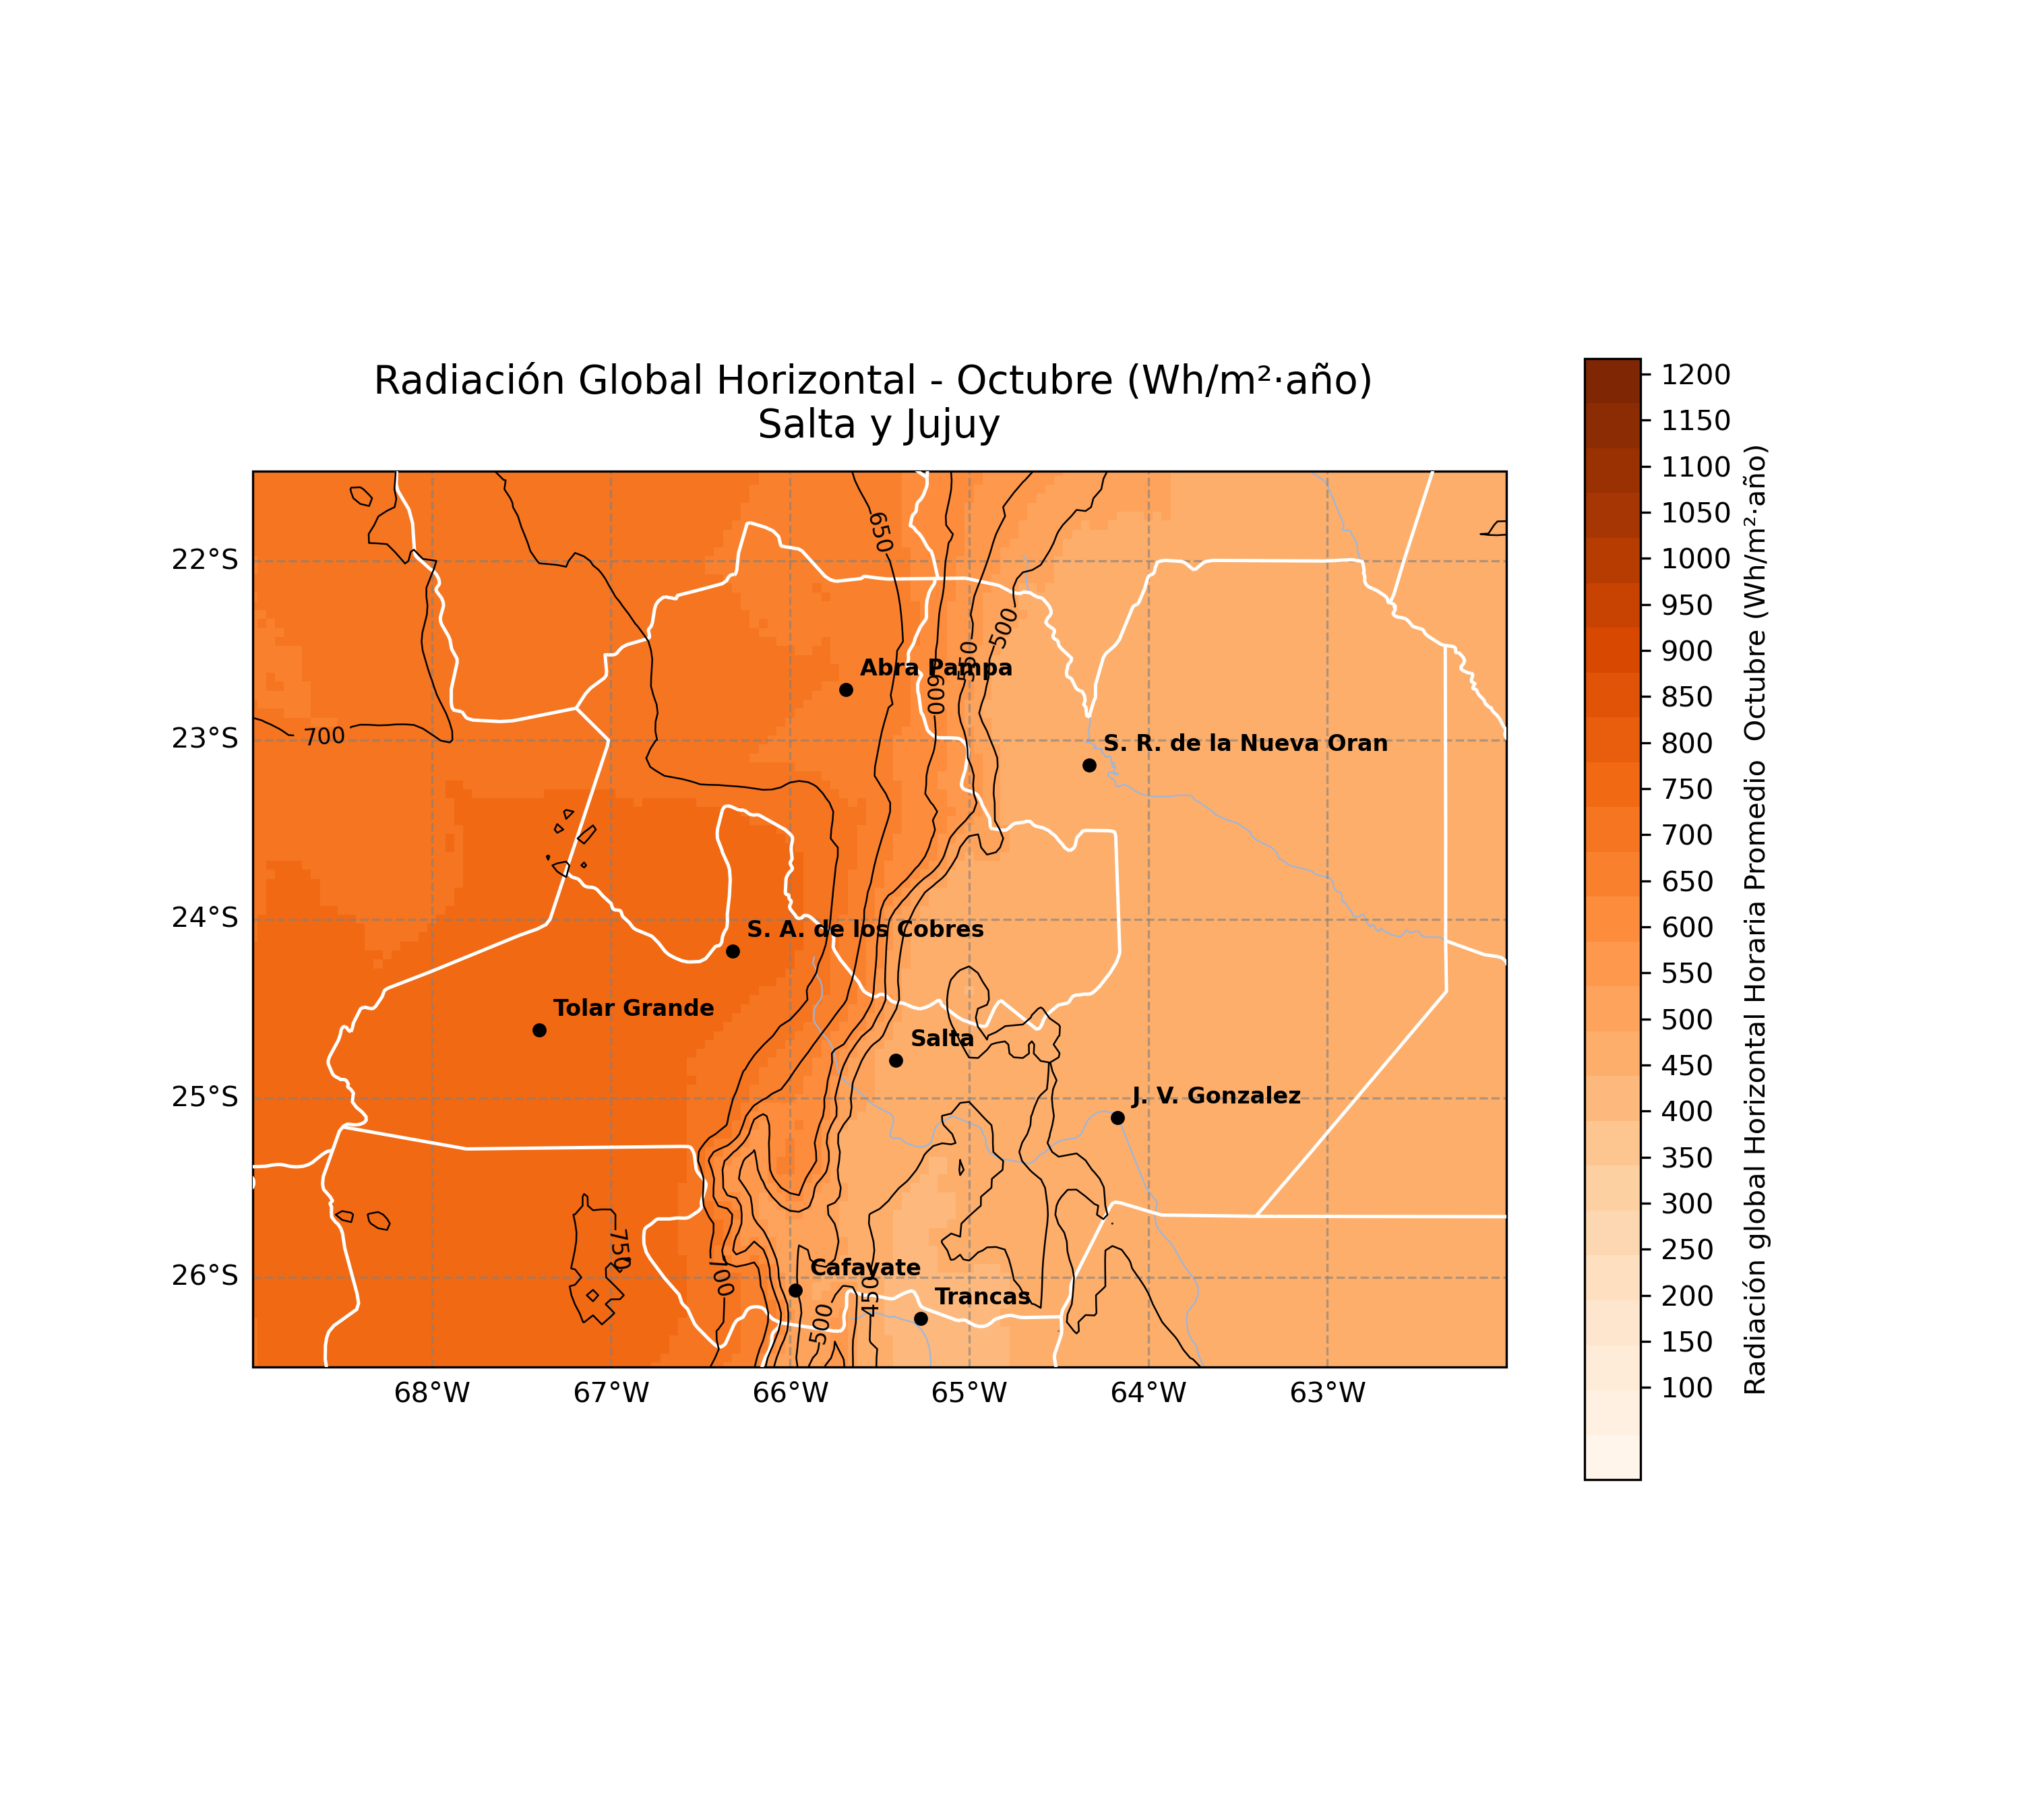
\includegraphics[width=0.99\textwidth]{figuras/Mapas/10_Octubre.png}
%DIFDELCMD < %%%
%DIFDELCMD < \caption{%
{%DIFAUXCMD
\DIFdelFL{Mapa de GHI medio mensual – Octubre (TMY).}}
%DIFAUXCMD
%DIFDELCMD < \end{figure}
%DIFDELCMD < 

%DIFDELCMD < \begin{figure}[H]
%DIFDELCMD < \centering
%DIFDELCMD < 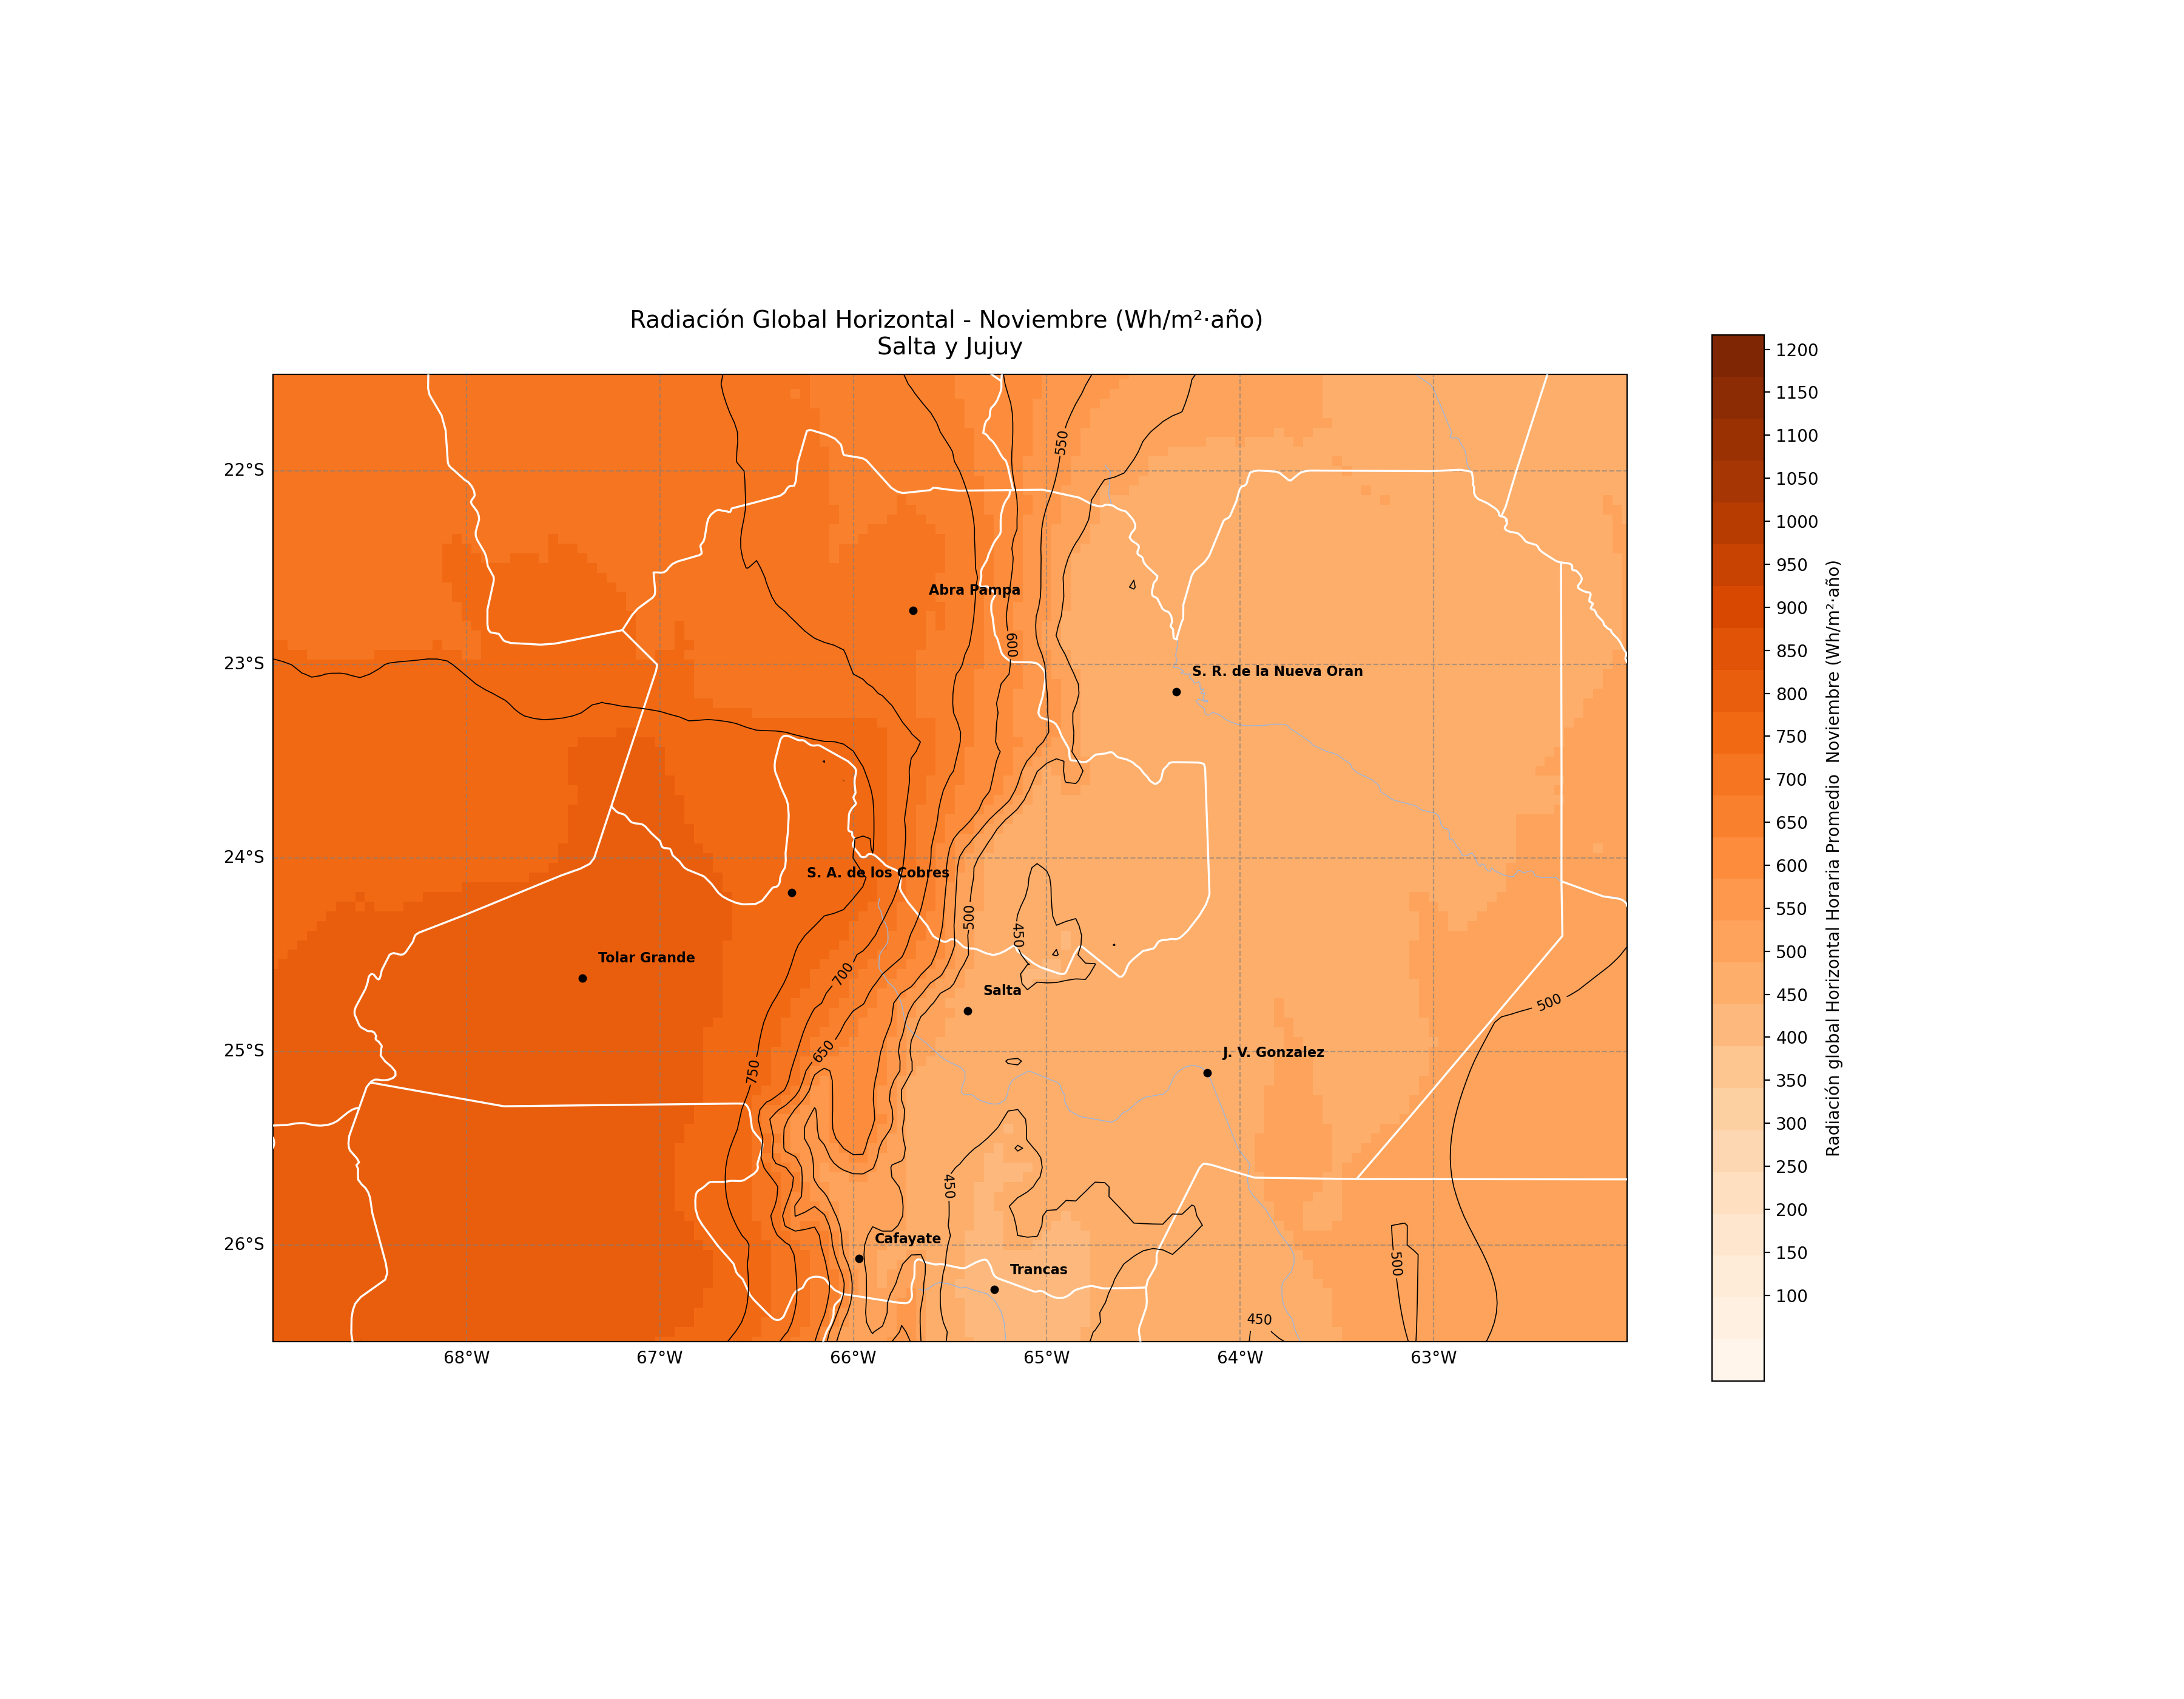
\includegraphics[width=0.99\textwidth]{figuras/Mapas/11_Noviembre.png}
%DIFDELCMD < %%%
%DIFDELCMD < \caption{%
{%DIFAUXCMD
\DIFdelFL{Mapa de GHI medio mensual – Noviembre (TMY).}}
%DIFAUXCMD
%DIFDELCMD < \end{figure}
%DIFDELCMD < 

%DIFDELCMD < \begin{figure}[H]
%DIFDELCMD < \centering
%DIFDELCMD < 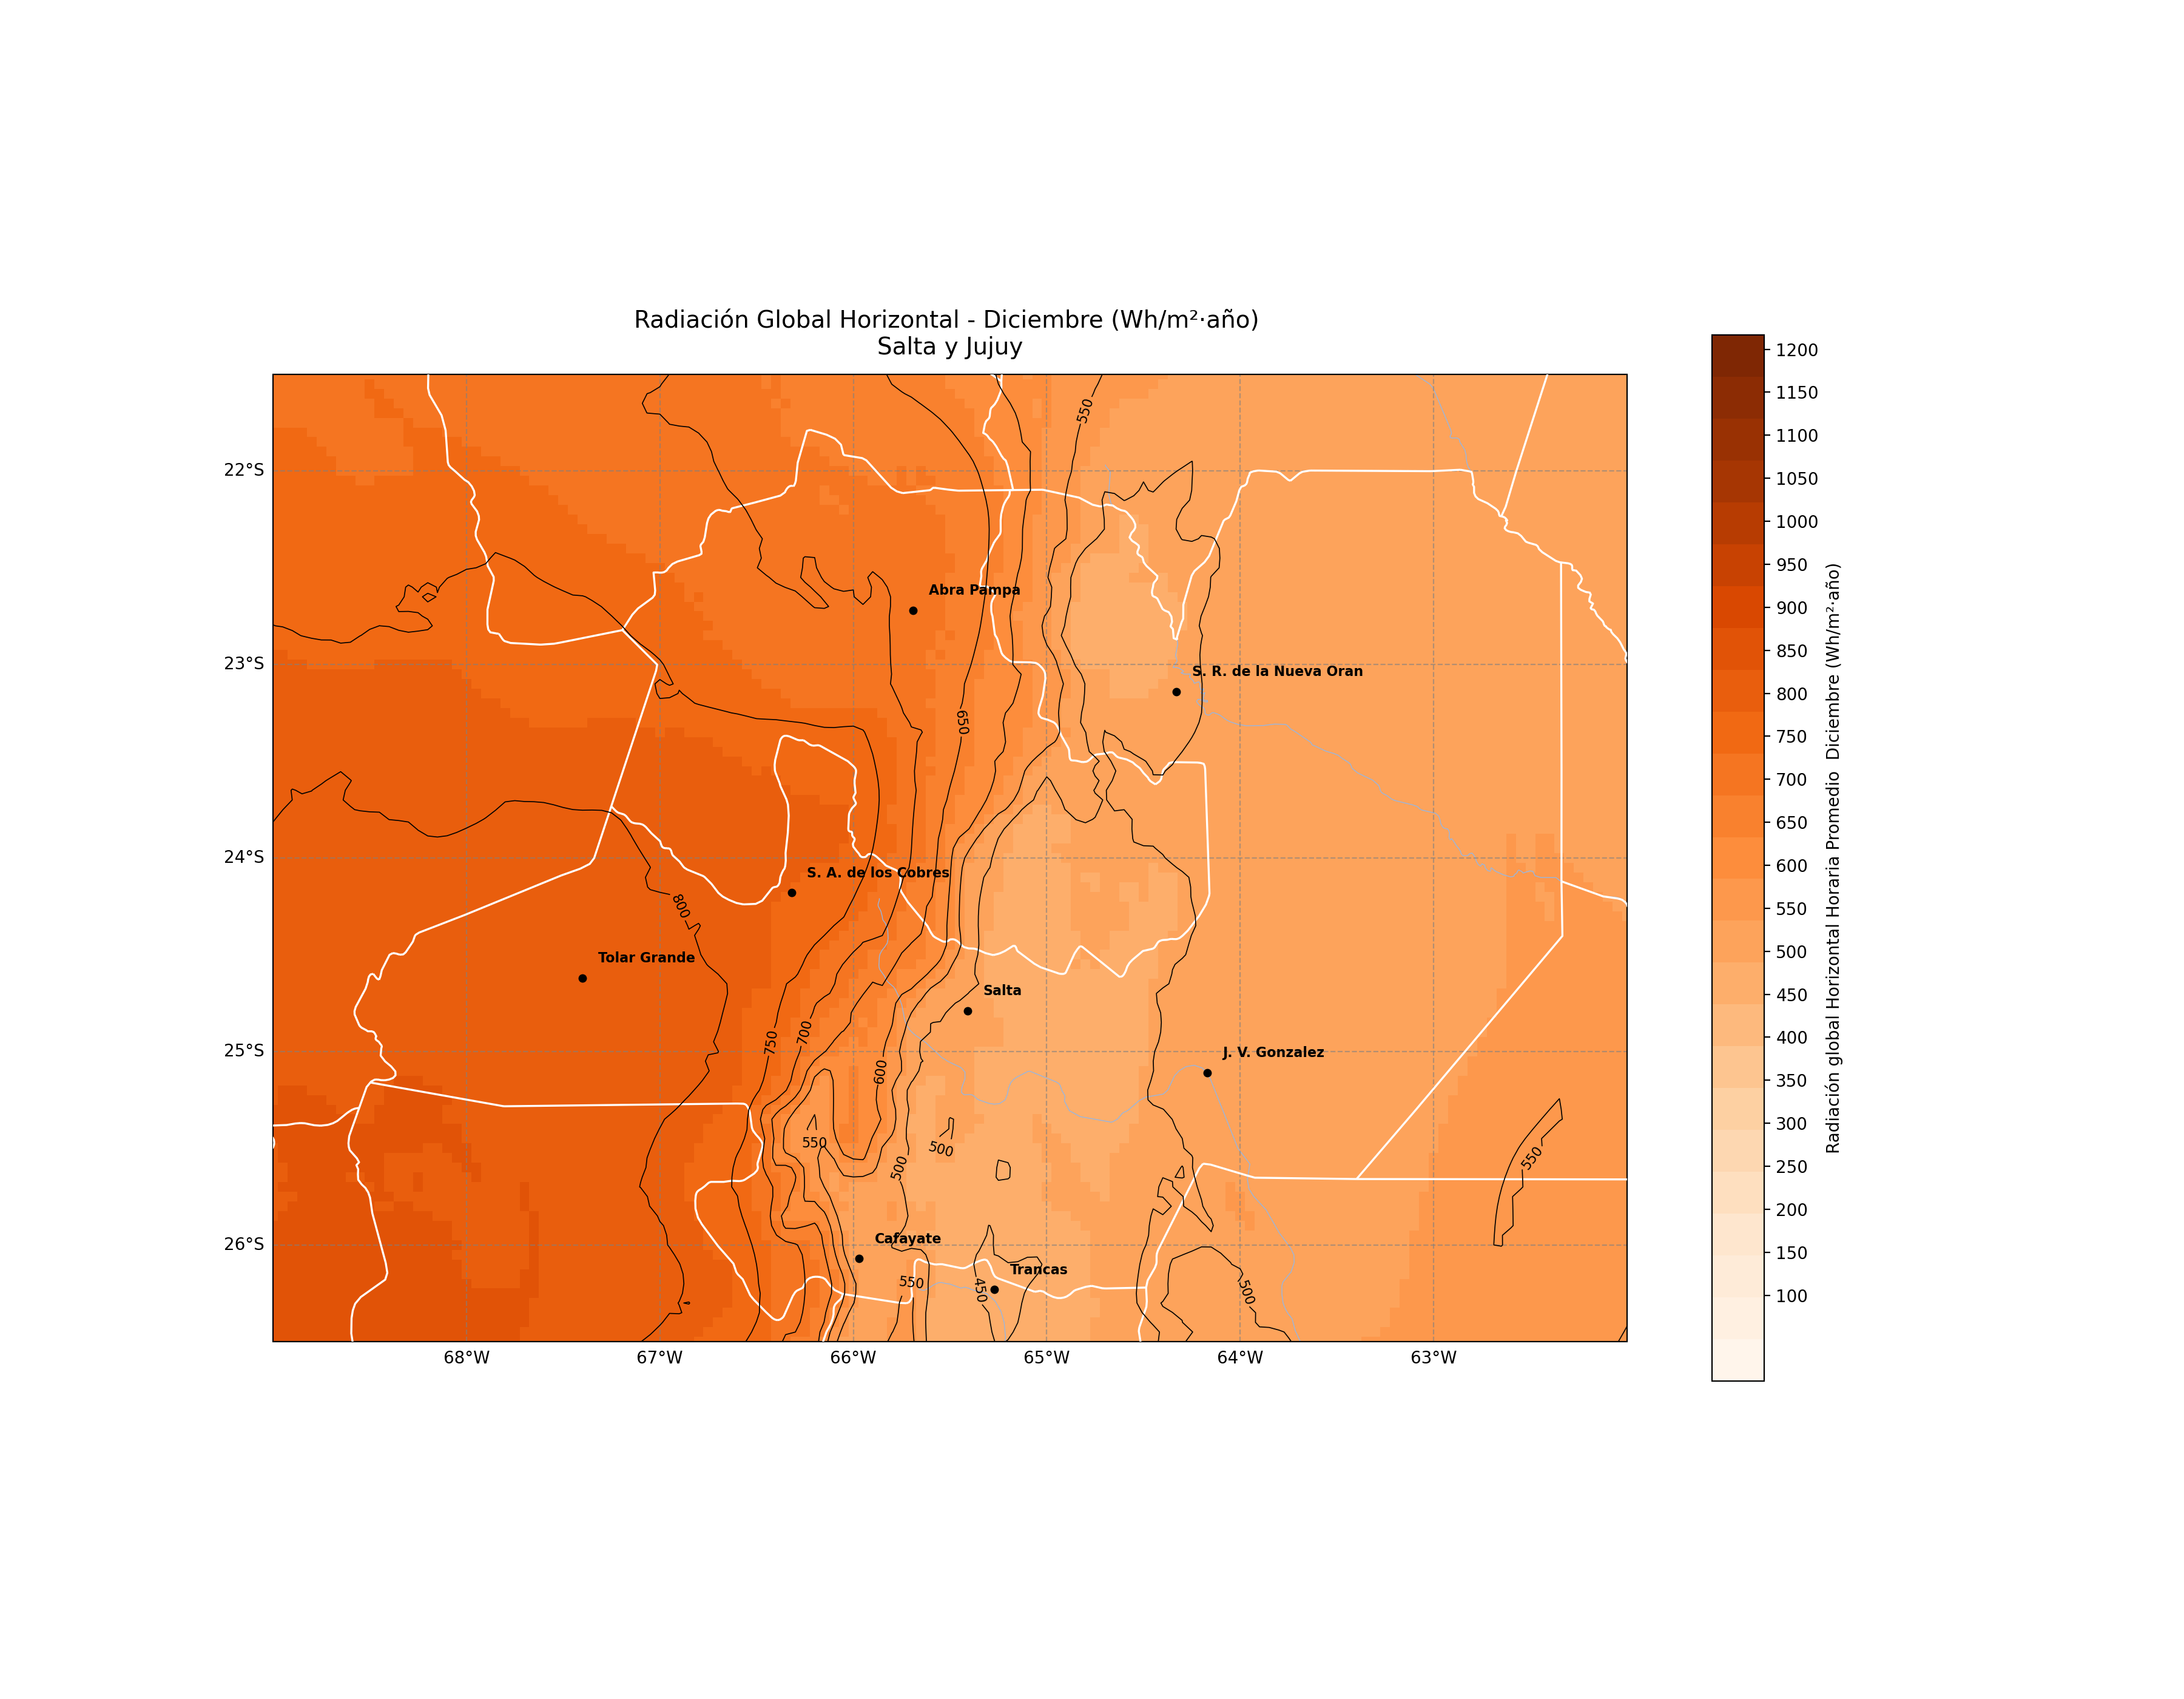
\includegraphics[width=0.99\textwidth]{figuras/Mapas/12_Diciembre.png}
%DIFDELCMD < %%%
%DIFDELCMD < \caption{%
{%DIFAUXCMD
\DIFdelFL{Mapa de GHI medio mensual – Diciembre (TMY).}}
%DIFAUXCMD
%DIFDELCMD < \end{figure}
%DIFDELCMD < 

%DIFDELCMD < \begin{figure}
%DIFDELCMD <     \centering	
%DIFDELCMD <         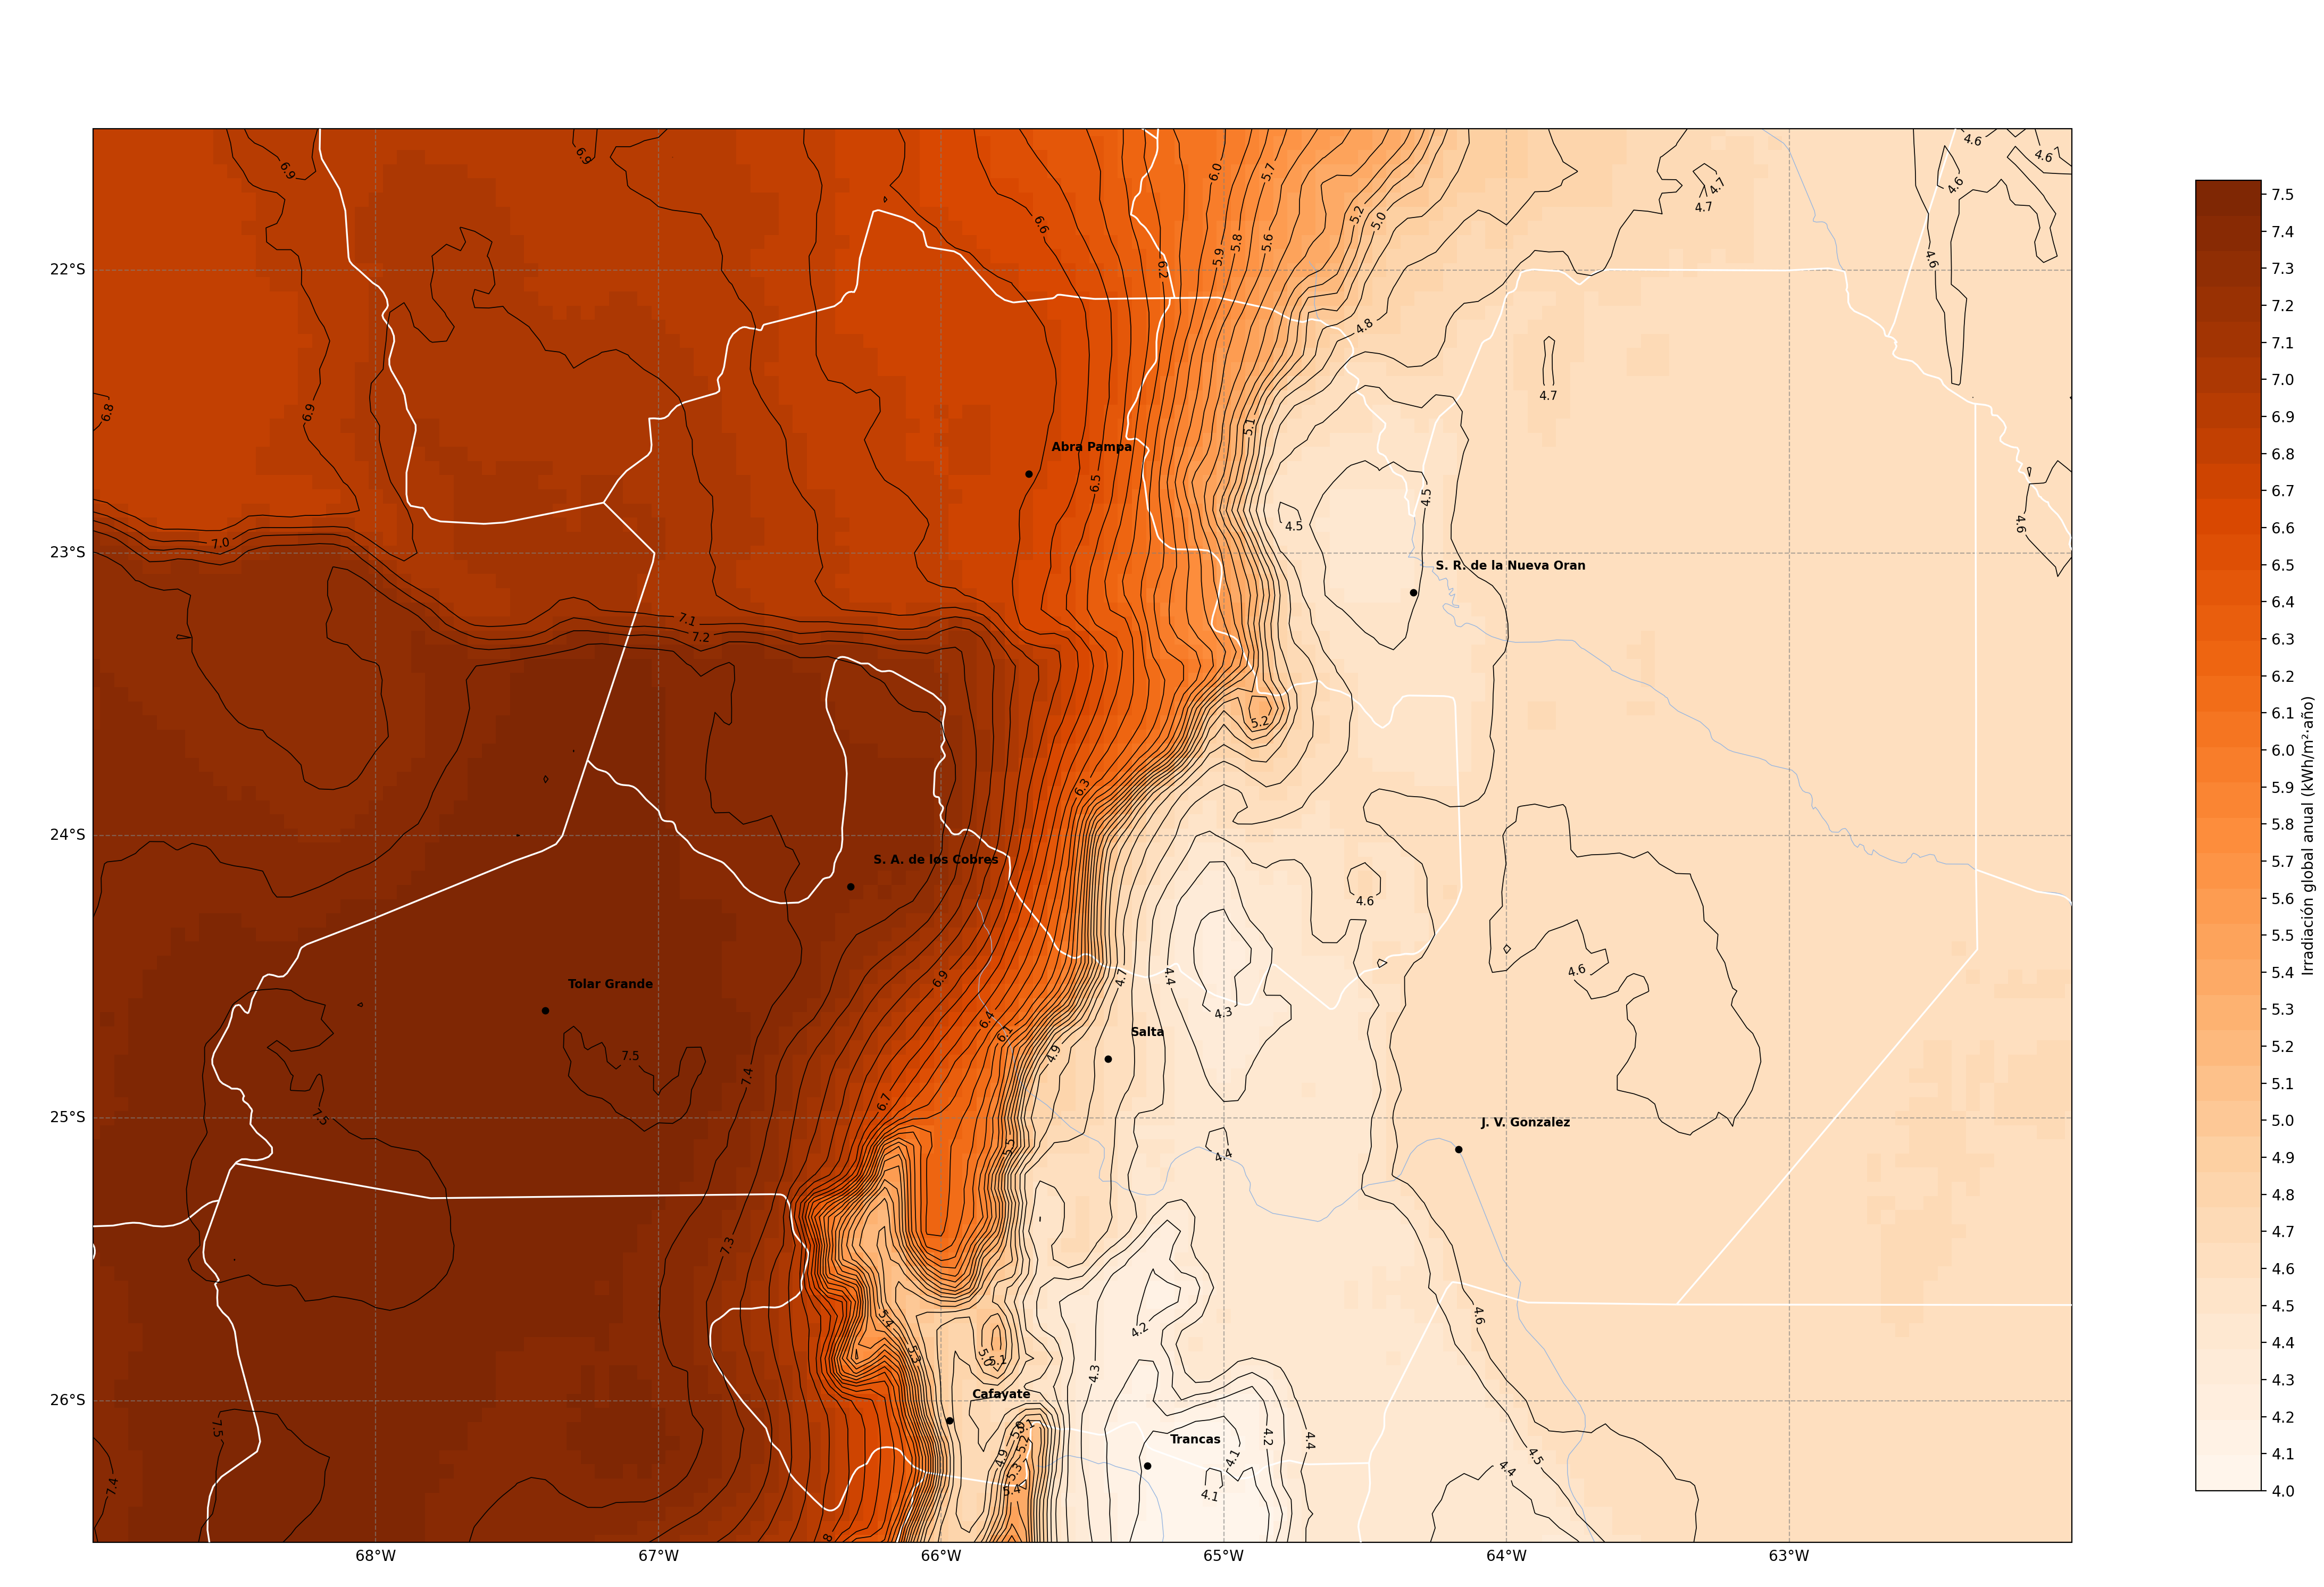
\includegraphics[width=0.99\textwidth]{figuras/Mapas/TMY.png}
%DIFDELCMD <     %%%
%DIFDELCMD < \caption{%
{%DIFAUXCMD
\DIFdelFL{TMY.}}
    %DIFAUXCMD
%DIFDELCMD < \label{fig:tmy}
%DIFDELCMD < \end{figure}
%DIFDELCMD < 

%DIFDELCMD <  \newpage  %%%
\DIFdelend \DIFaddbegin \addcontentsline{toc}{chapter}{\textbf{Anexo 1}} 
\lhead{Anexo 1}
\rhead{\newtitle}
\cfoot{\thepage}
\renewcommand{\headrulewidth}{1pt}
\renewcommand{\footrulewidth}{1pt}

\chapter*{Anexo 2}


\noindent \textbf{Mapas de GHI derivados del proceso de adaptación al sitio}.

Una de las herramientas ampliamente en la caracterización del recurso solar son sin dudas los mapas que explican de manera rápida e intuitiva de cómo distribuye el recurso en una región. La construcción de estos ha sido ampliamente estudiada en diversas partes del mundo debido a su utilidad en distintas áreas de aplicaciones. Particularmente en Argentina dentro de la Guía del Recurso Solar publicada por la Secretaría de Energía se distribuye el ATLAS DE ENERGÍA SOLAR DE LA REPÚBLICA ARGENTINA que indica la distribución espacial del promedio de la irradianción solar global diaria sobre un plano horizontal discriminada por mes trazándose las isolíneas correspondientes a cada mes y al año
espaciadas 0.5 kWh/m2. Una aproximación de esto implementada para el Noroeste Argentino es el TRAZADO DE MAPAS MEDIOS ANUALES DE ENERGÍA SOLAR GLOBAL, DIRECTA, DIFUSA Y TILT, USANDO LA BASE DE DATOS DE SWERA. CASO DE ESTUDIO: PROVINCIAS DE SALTA Y JUJUY. Donde se presentan mapas de líneas de iso-irradiación solar global media anual para las provincias de Salta y Jujuy utilizando los datos dela base satelital SWERA, cuyas celdas son cuadrados de 40 km. de lado, a través del método geoestadístico del kriging y un variograma lineal. 


Además de la utilidad evidente de los mapas mensuales de irradiación, resulta imprescindible incorporar un Año Meteorológico Típico (TMY, por sus siglas en inglés) como insumo fundamental para la caracterización robusta del recurso solar. El TMY permite condensar en un solo año sintético las condiciones climáticas representativas de un período histórico más extenso, evitando que la evaluación dependa de anomalías o eventos extremos propios de años particulares. Esta aproximación garantiza que los análisis derivados —ya sean energéticos, estadísticos o de diseño— se apoyen en una base climatológica estable y científicamente defendible.

El empleo de un TMY contribuye, asimismo, a mejorar la comparabilidad de los resultados entre regiones y entre distintos estudios. Dado que constituye un estándar internacionalmente aceptado en la industria solar, su utilización asegura que la interpretación de los mapas y métricas derivadas no se vea afectada por variaciones interanuales propias de la dinámica atmosférica. En consecuencia, los mapas mensuales construidos a partir de un TMY adquieren una mayor validez para estudios de planificación y apoyo a políticas públicas.


La construcción del TMY fue realizado exclusivamente a partir de la GHI, como el obtenido mediante el método de Finkelstein–Schafer con procesamiento vectorizado, constituye un paso metodológico plenamente válido y científicamente justificado cuando el objetivo central es la caracterización espacial del recurso solar. La GHI sintetiza la mayor parte de la variabilidad radiativa relevante para estudios de disponibilidad energética, por lo que disponer de un TMY específico para esta variable permite estabilizar dicha variabilidad y evitar que los mapas mensuales se vean distorsionados por fluctuaciones episódicas asociadas a años inusualmente nublados o excepcionalmente despejados. Esto adquiere especial relevancia en regiones subtropicales o de topografía compleja, donde la variabilidad interanual puede ser significativa.

El uso del método Finkelstein–Schafer para la selección del TMY garantiza que el año sintético conserve, para cada mes, la forma estadística de la distribución horaria de GHI, reproduciendo fielmente las colas, percentiles y patrones de dispersión que caracterizan al clima local. Este enfoque es particularmente robusto cuando se trabaja con series extensas y heterogéneas, como las derivadas de bases satelitales corregidas, y es compatible con la construcción de productos espaciales como mapas mensuales, dado que preserva la coherencia entre celdas y evita la introducción de discontinuidades artificiales. Por ello, aun con una única variable radiativa, el TMY aporta una base homogénea sobre la cual montar comparaciones y análisis espaciales.

Además, la necesidad de un TMY se intensifica al trabajar con interpolaciones espaciales o con métodos geoestadísticos —como kriging sobre mallas satelitales—, ya que estos algoritmos dependen críticamente de la estabilidad estadística de los datos de entrada. En ausencia de un TMY, un año particular podría inducir gradientes irreales o sesgos en las isolíneas mensuales, comprometiendo la interpretación de los patrones de irradiación. En contraste, un TMY asegura que los mapas reflejen la climatología promedio y no el comportamiento anómalo de un subconjunto temporal limitado. De este modo, se mejora la calidad cartográfica y se preserva la relevancia física de las estructuras espaciales observadas.

Asimismo, la integración del TMY con la metodología de site adaptation —previamente discutida— permite extender de forma consistente los resultados hacia regiones con escasa instrumentación o alta dependencia de datos satelitales corregidos. El TMY actúa como un marco de referencia climatológico uniforme que facilita compatibilizar las adaptaciones por sitio con la estructura estadística regional, evitando que cada mapa mensual responda a patrones temporales idiosincráticos que dificulten su comparación transversal. Esto se traduce en una herramienta más robusta para estudios de sensibilidad, validación regional y análisis de desempeño energético.

Finalmente, la generación de los doce mapas mensuales de GHI media basados en el TMY obtenido no solo preserva la representatividad climatológica del recurso, sino que también proporciona una base metodológica sólida para estudios comparativos, planificación energética y análisis de potencial solar. De este modo, los mapas presentados se apoyan en una estructura temporal sintetizada que retiene las características más recurrentes y fundamentales del clima radiativo regional, cumpliendo con los estándares habituales de la literatura internacional en recursos solares y reforzando la credibilidad científica de los productos cartográficos derivados.



A continuación se presentan los doce mapas mensuales de la Irradiación Global Horizontal (GHI) obtenidos a partir del Año Meteorológico Típico (TMY), resultantes del proceso de adaptación al sitio.

\begin{figure}[H]
\centering
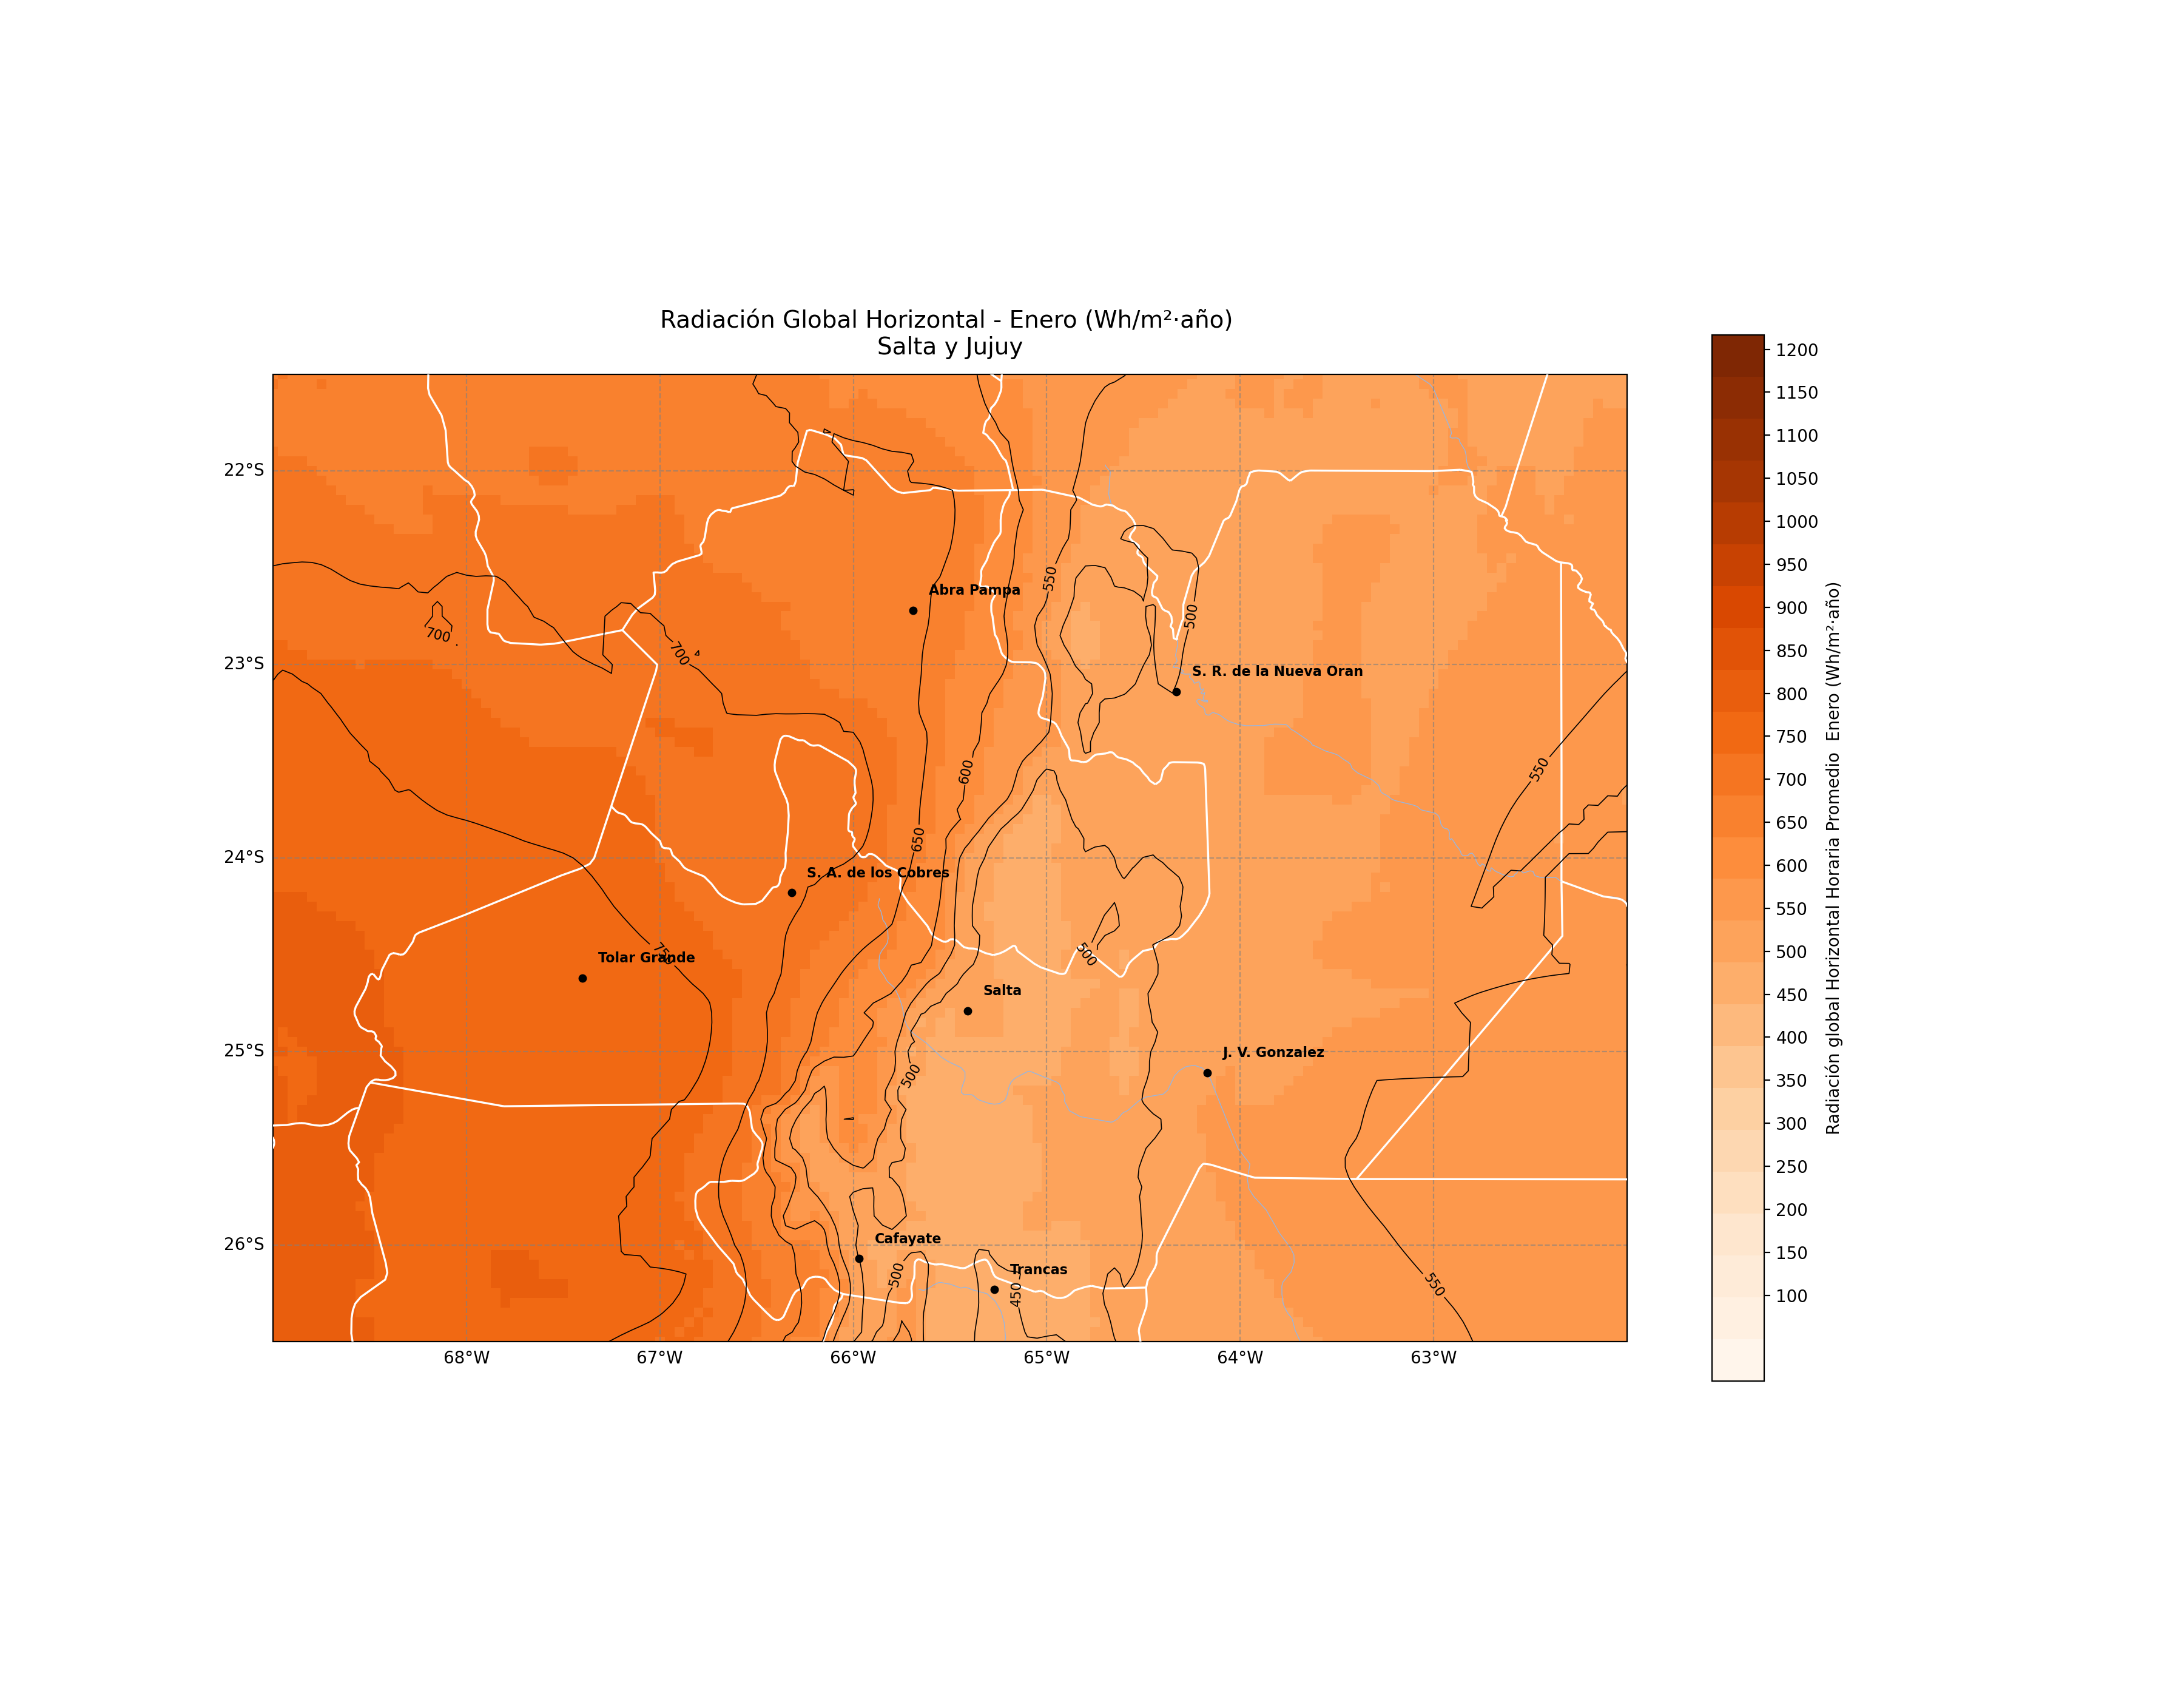
\includegraphics[width=0.95\textwidth]{figuras/Mapas/1_Enero.png}
\caption{Mapa de GHI medio mensual – Enero (TMY).}
\end{figure}

\begin{figure}[H]
\centering
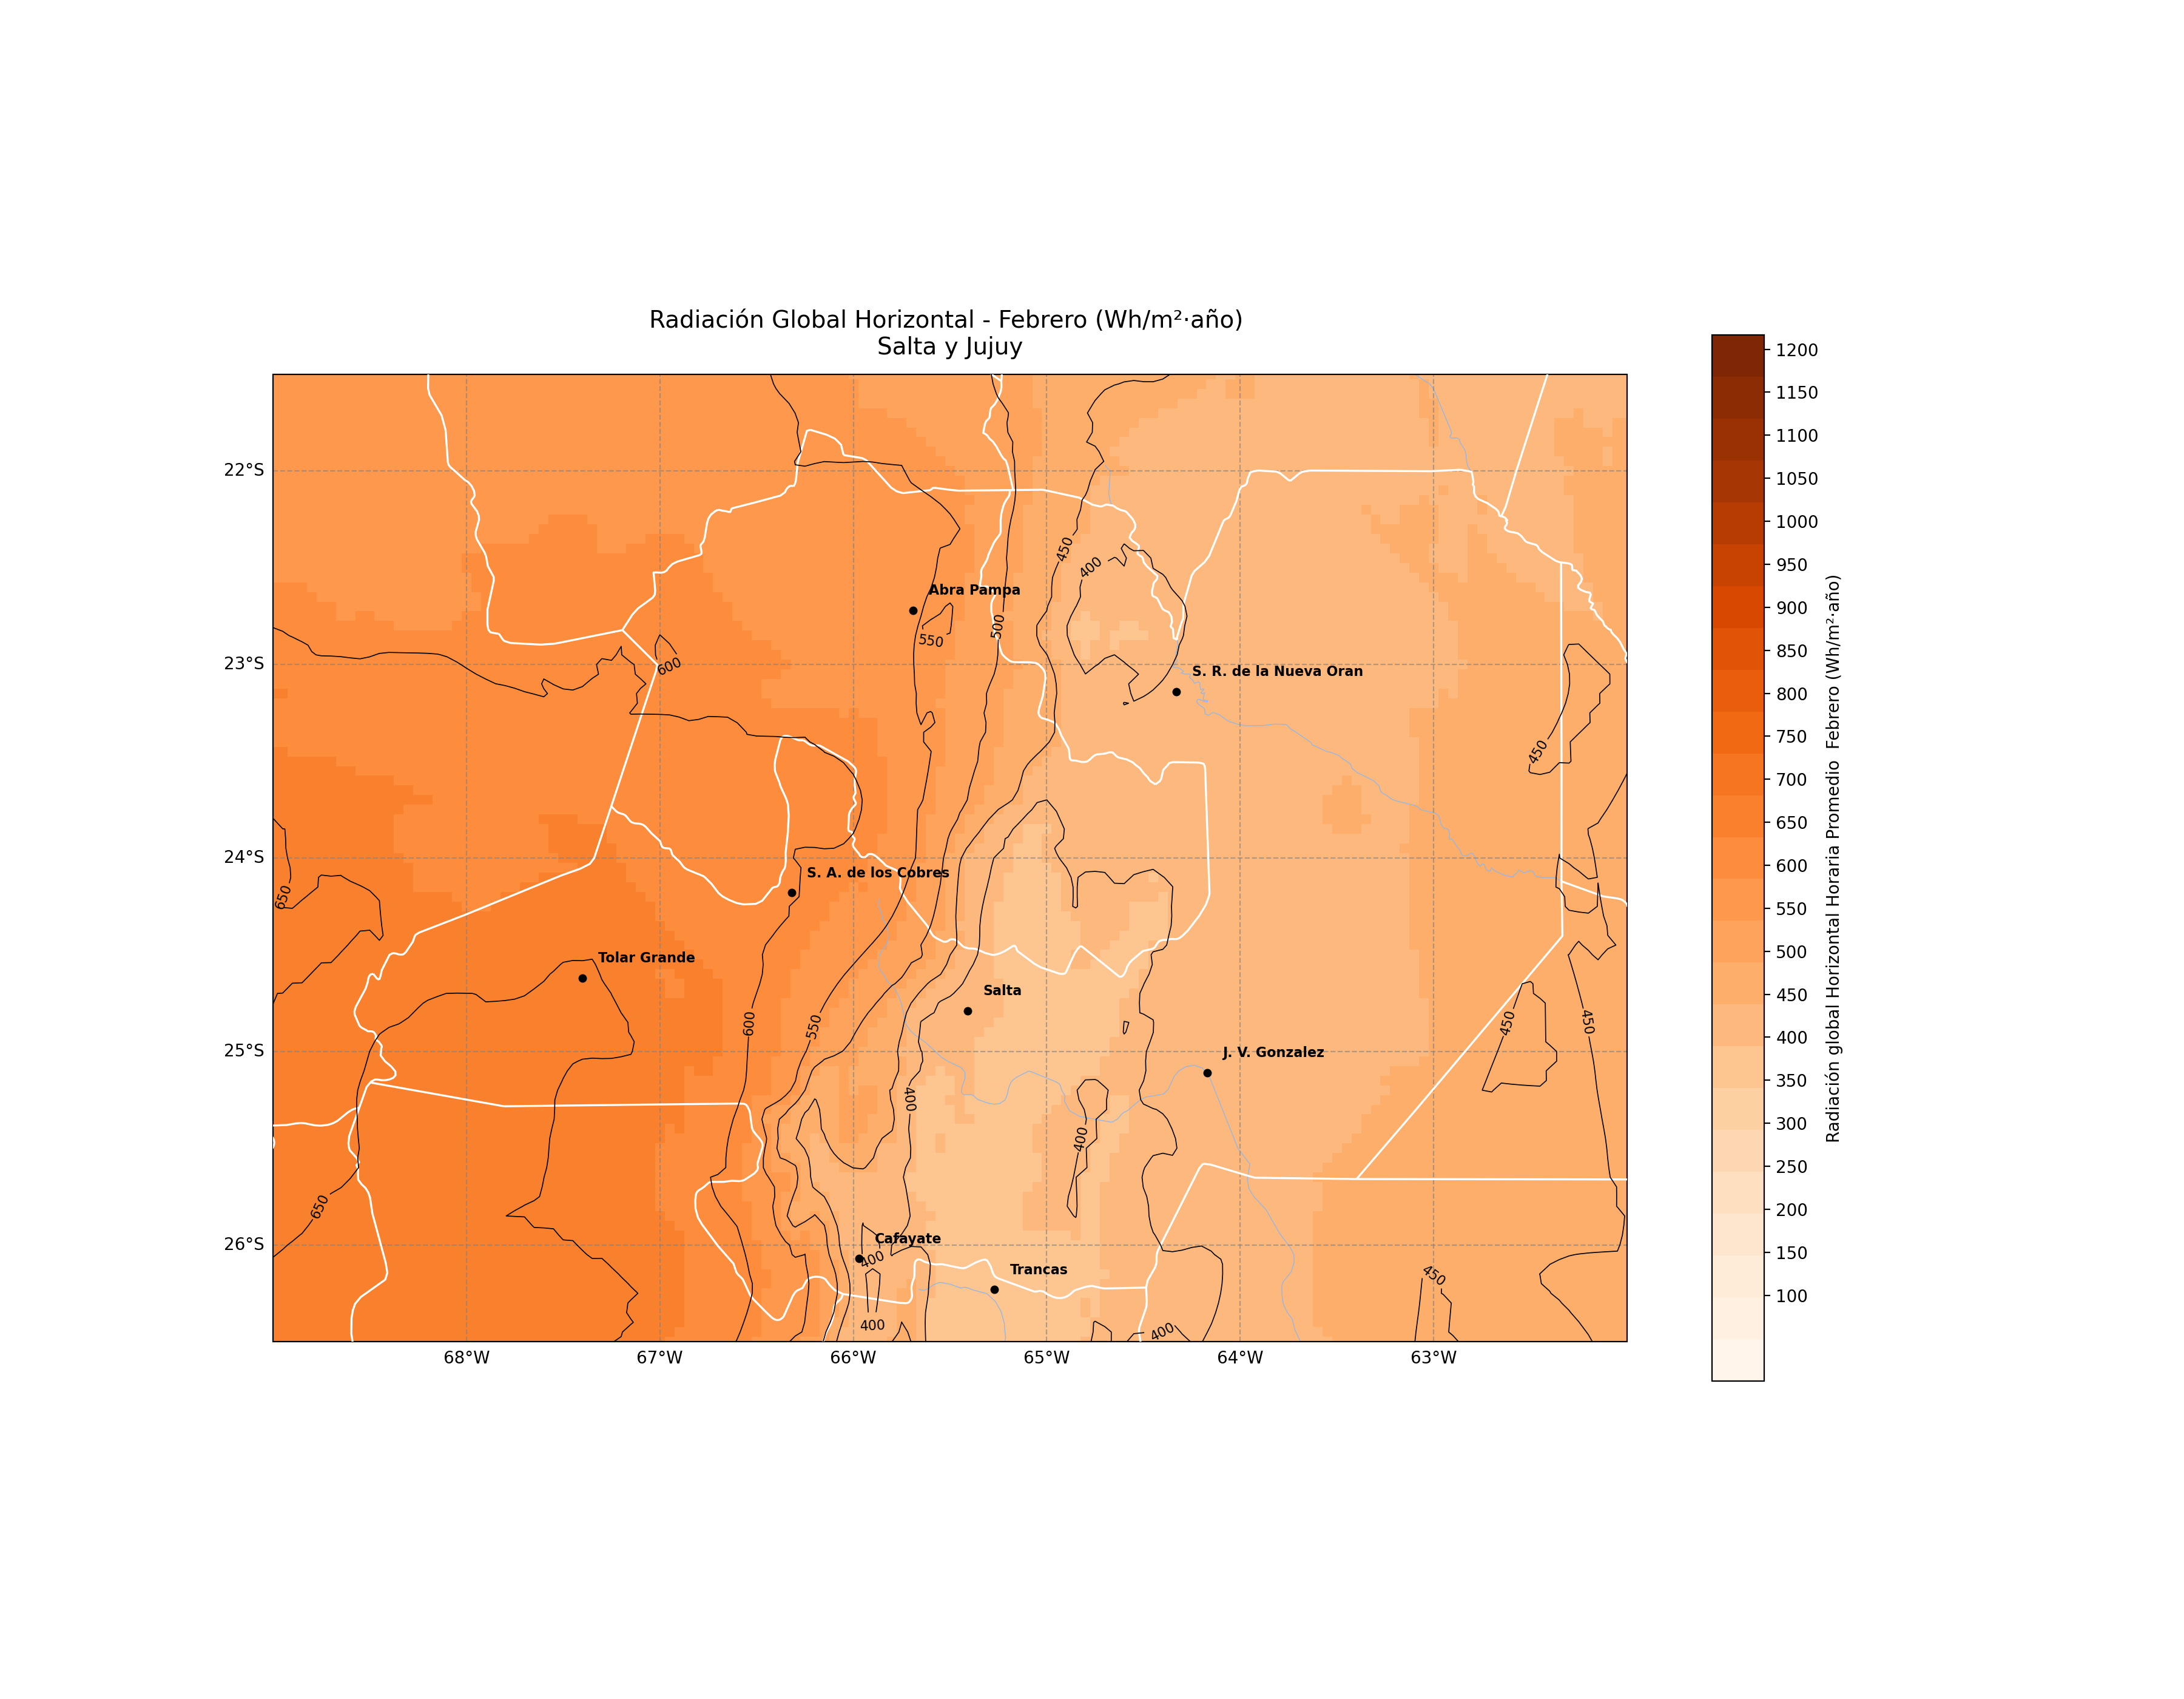
\includegraphics[width=0.95\textwidth]{figuras/Mapas/2_Febrero.png}
\caption{Mapa de GHI medio mensual – Febrero (TMY).}
\end{figure}

\begin{figure}[H]
\centering
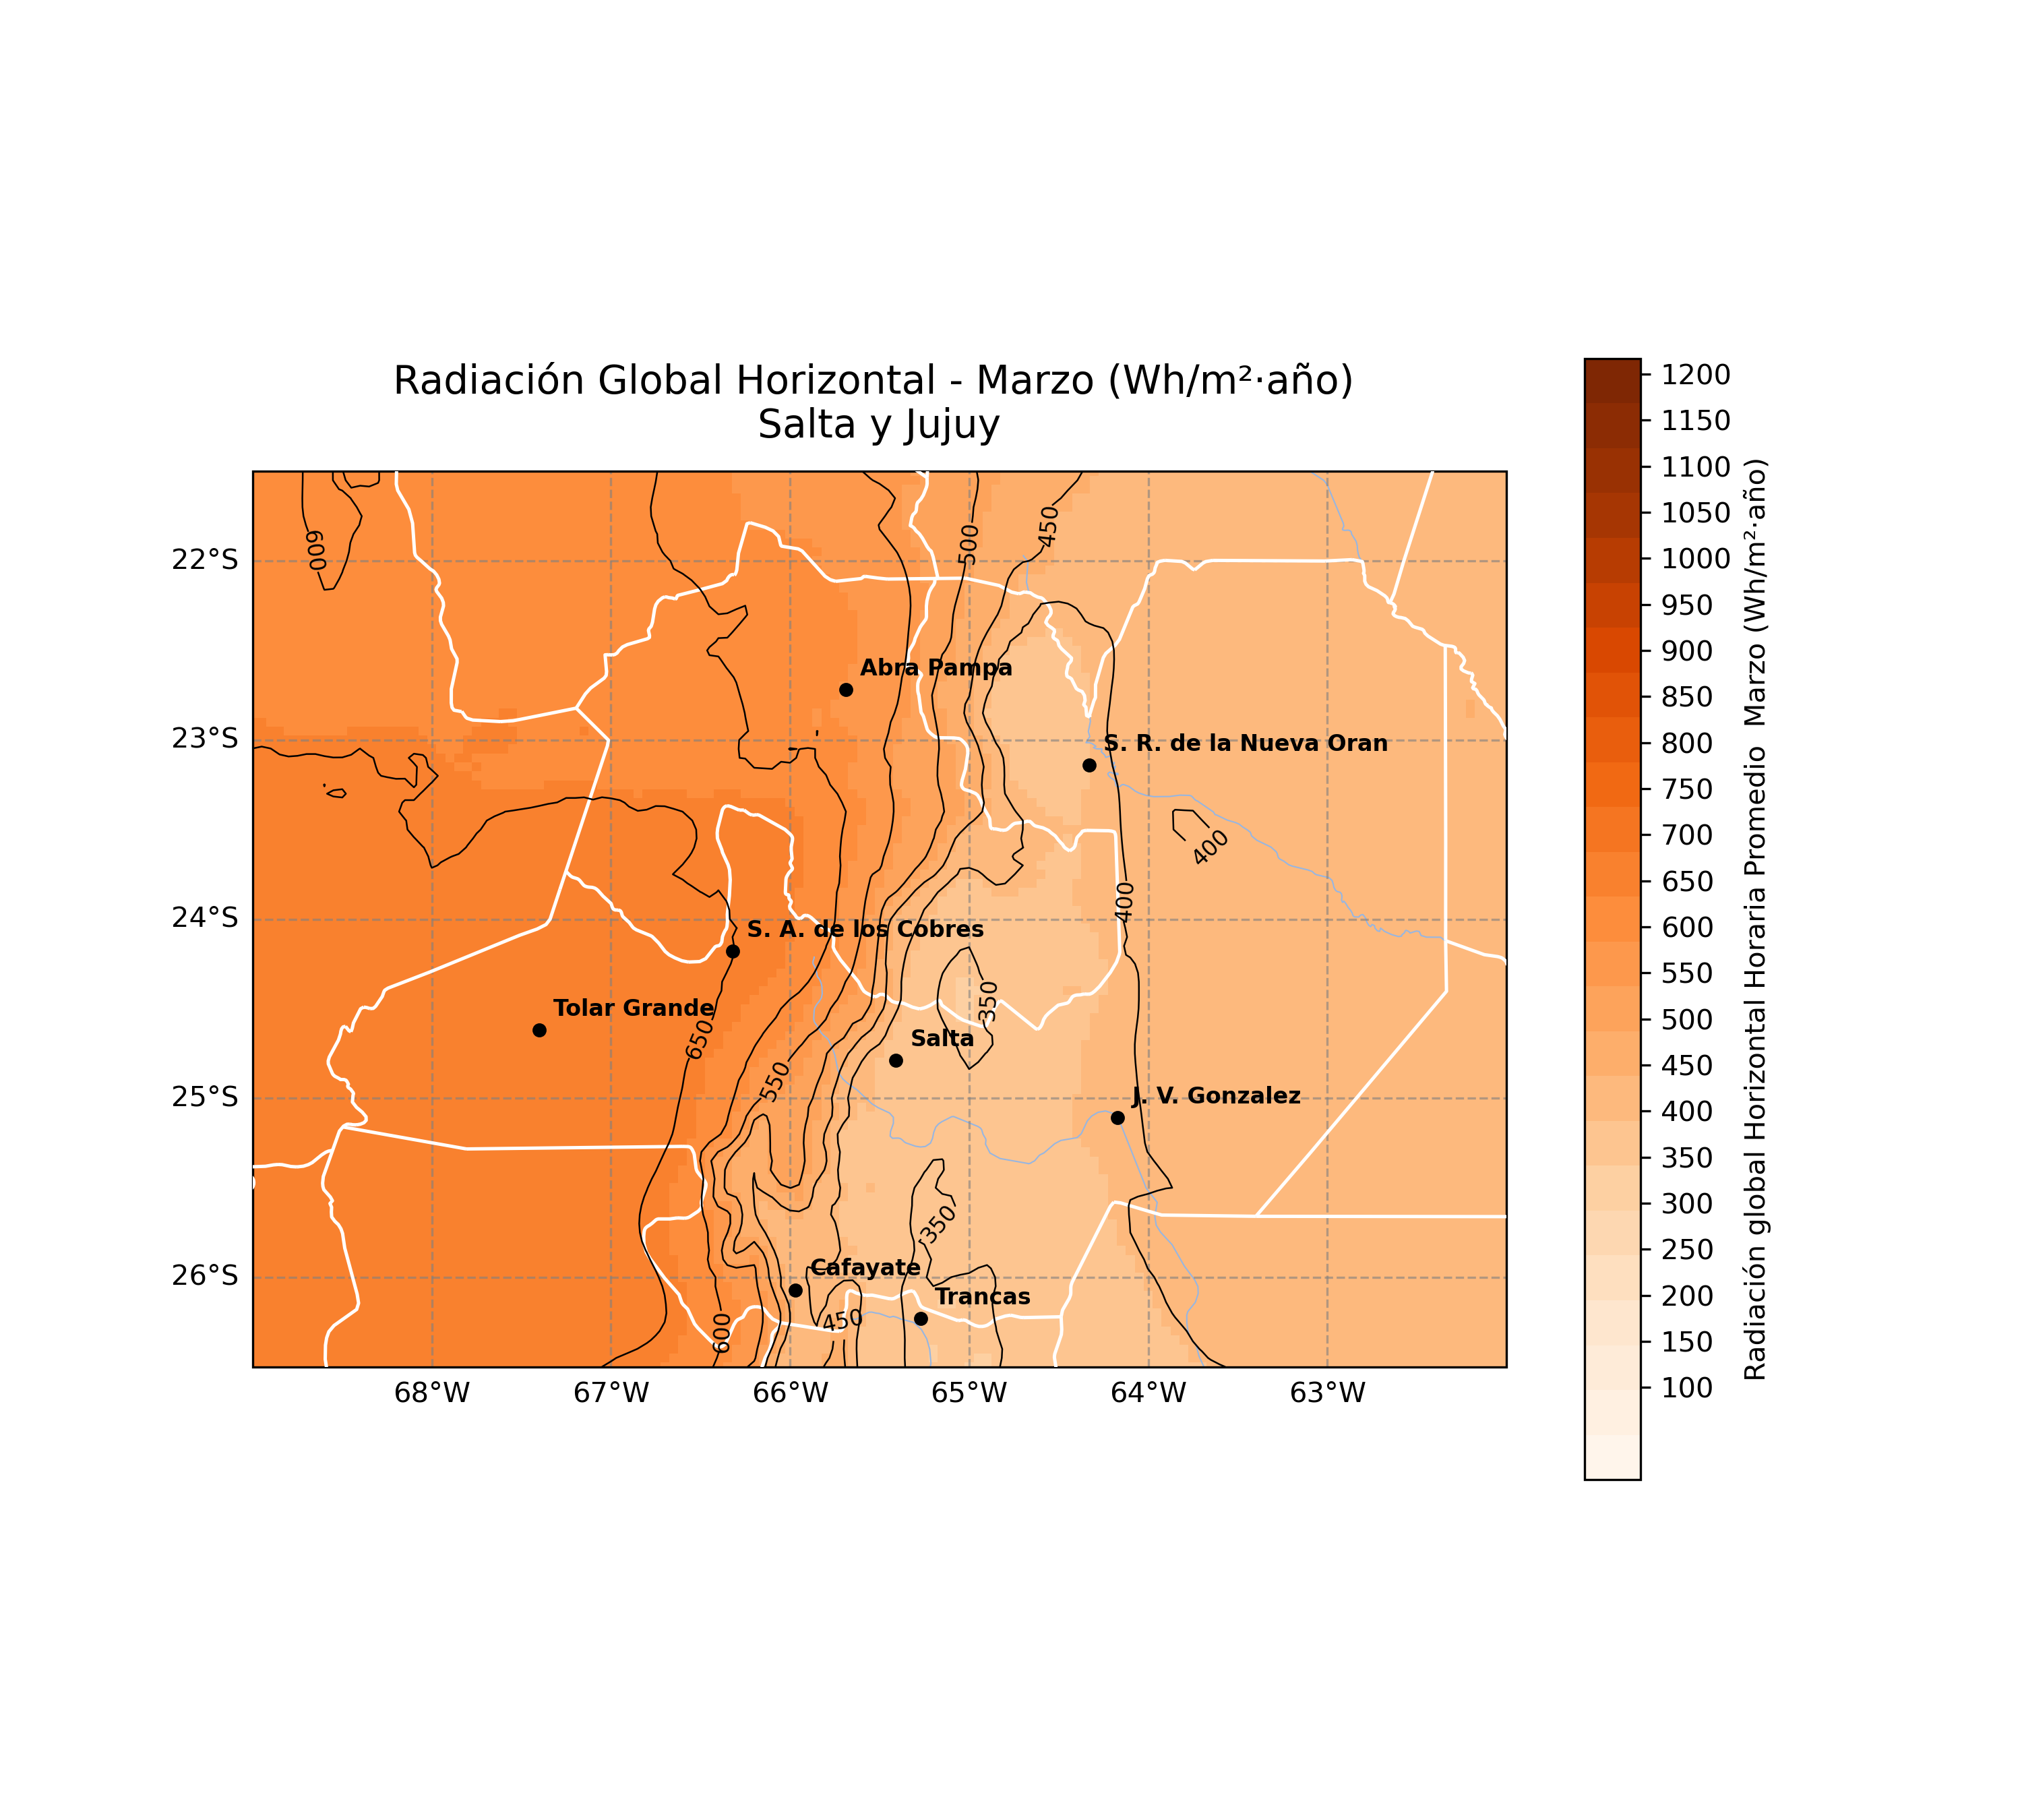
\includegraphics[width=0.95\textwidth]{figuras/Mapas/3_Marzo.png}
\caption{Mapa de GHI medio mensual – Marzo (TMY).}
\end{figure}

\begin{figure}[H]
\centering
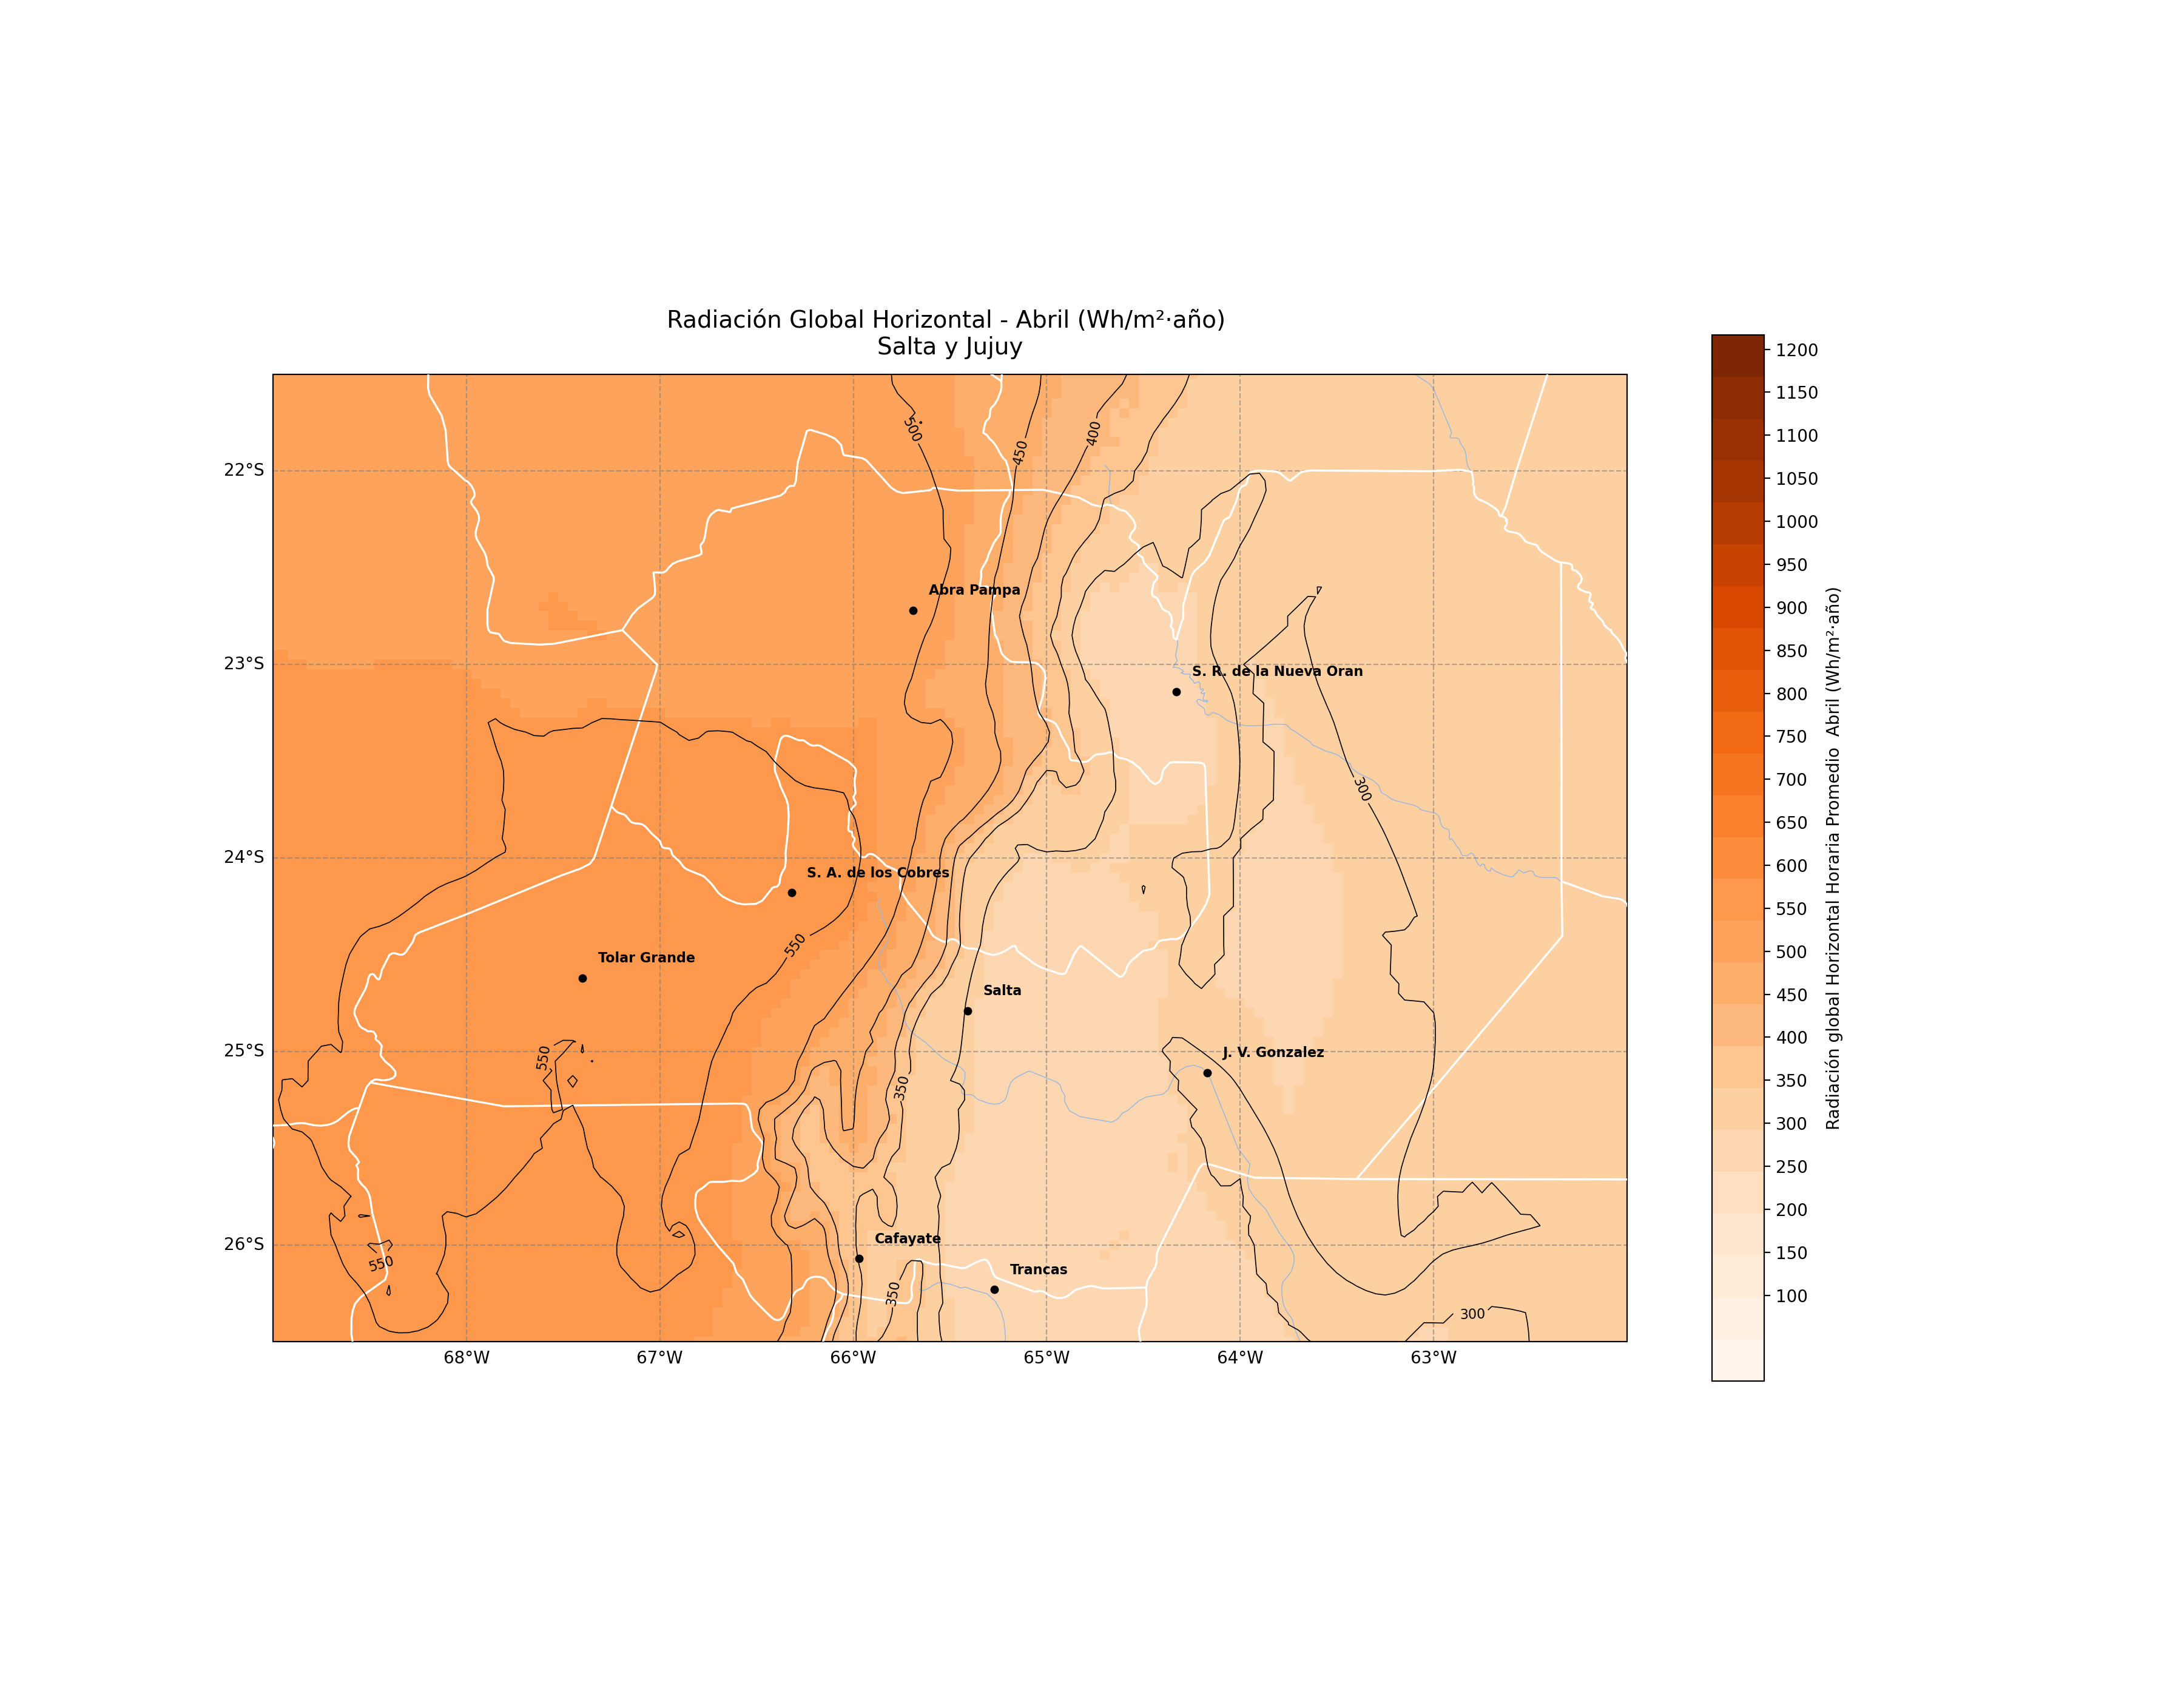
\includegraphics[width=0.95\textwidth]{figuras/Mapas/4_Abril.png}
\caption{Mapa de GHI medio mensual – Abril (TMY).}
\end{figure}

\begin{figure}[H]
\centering
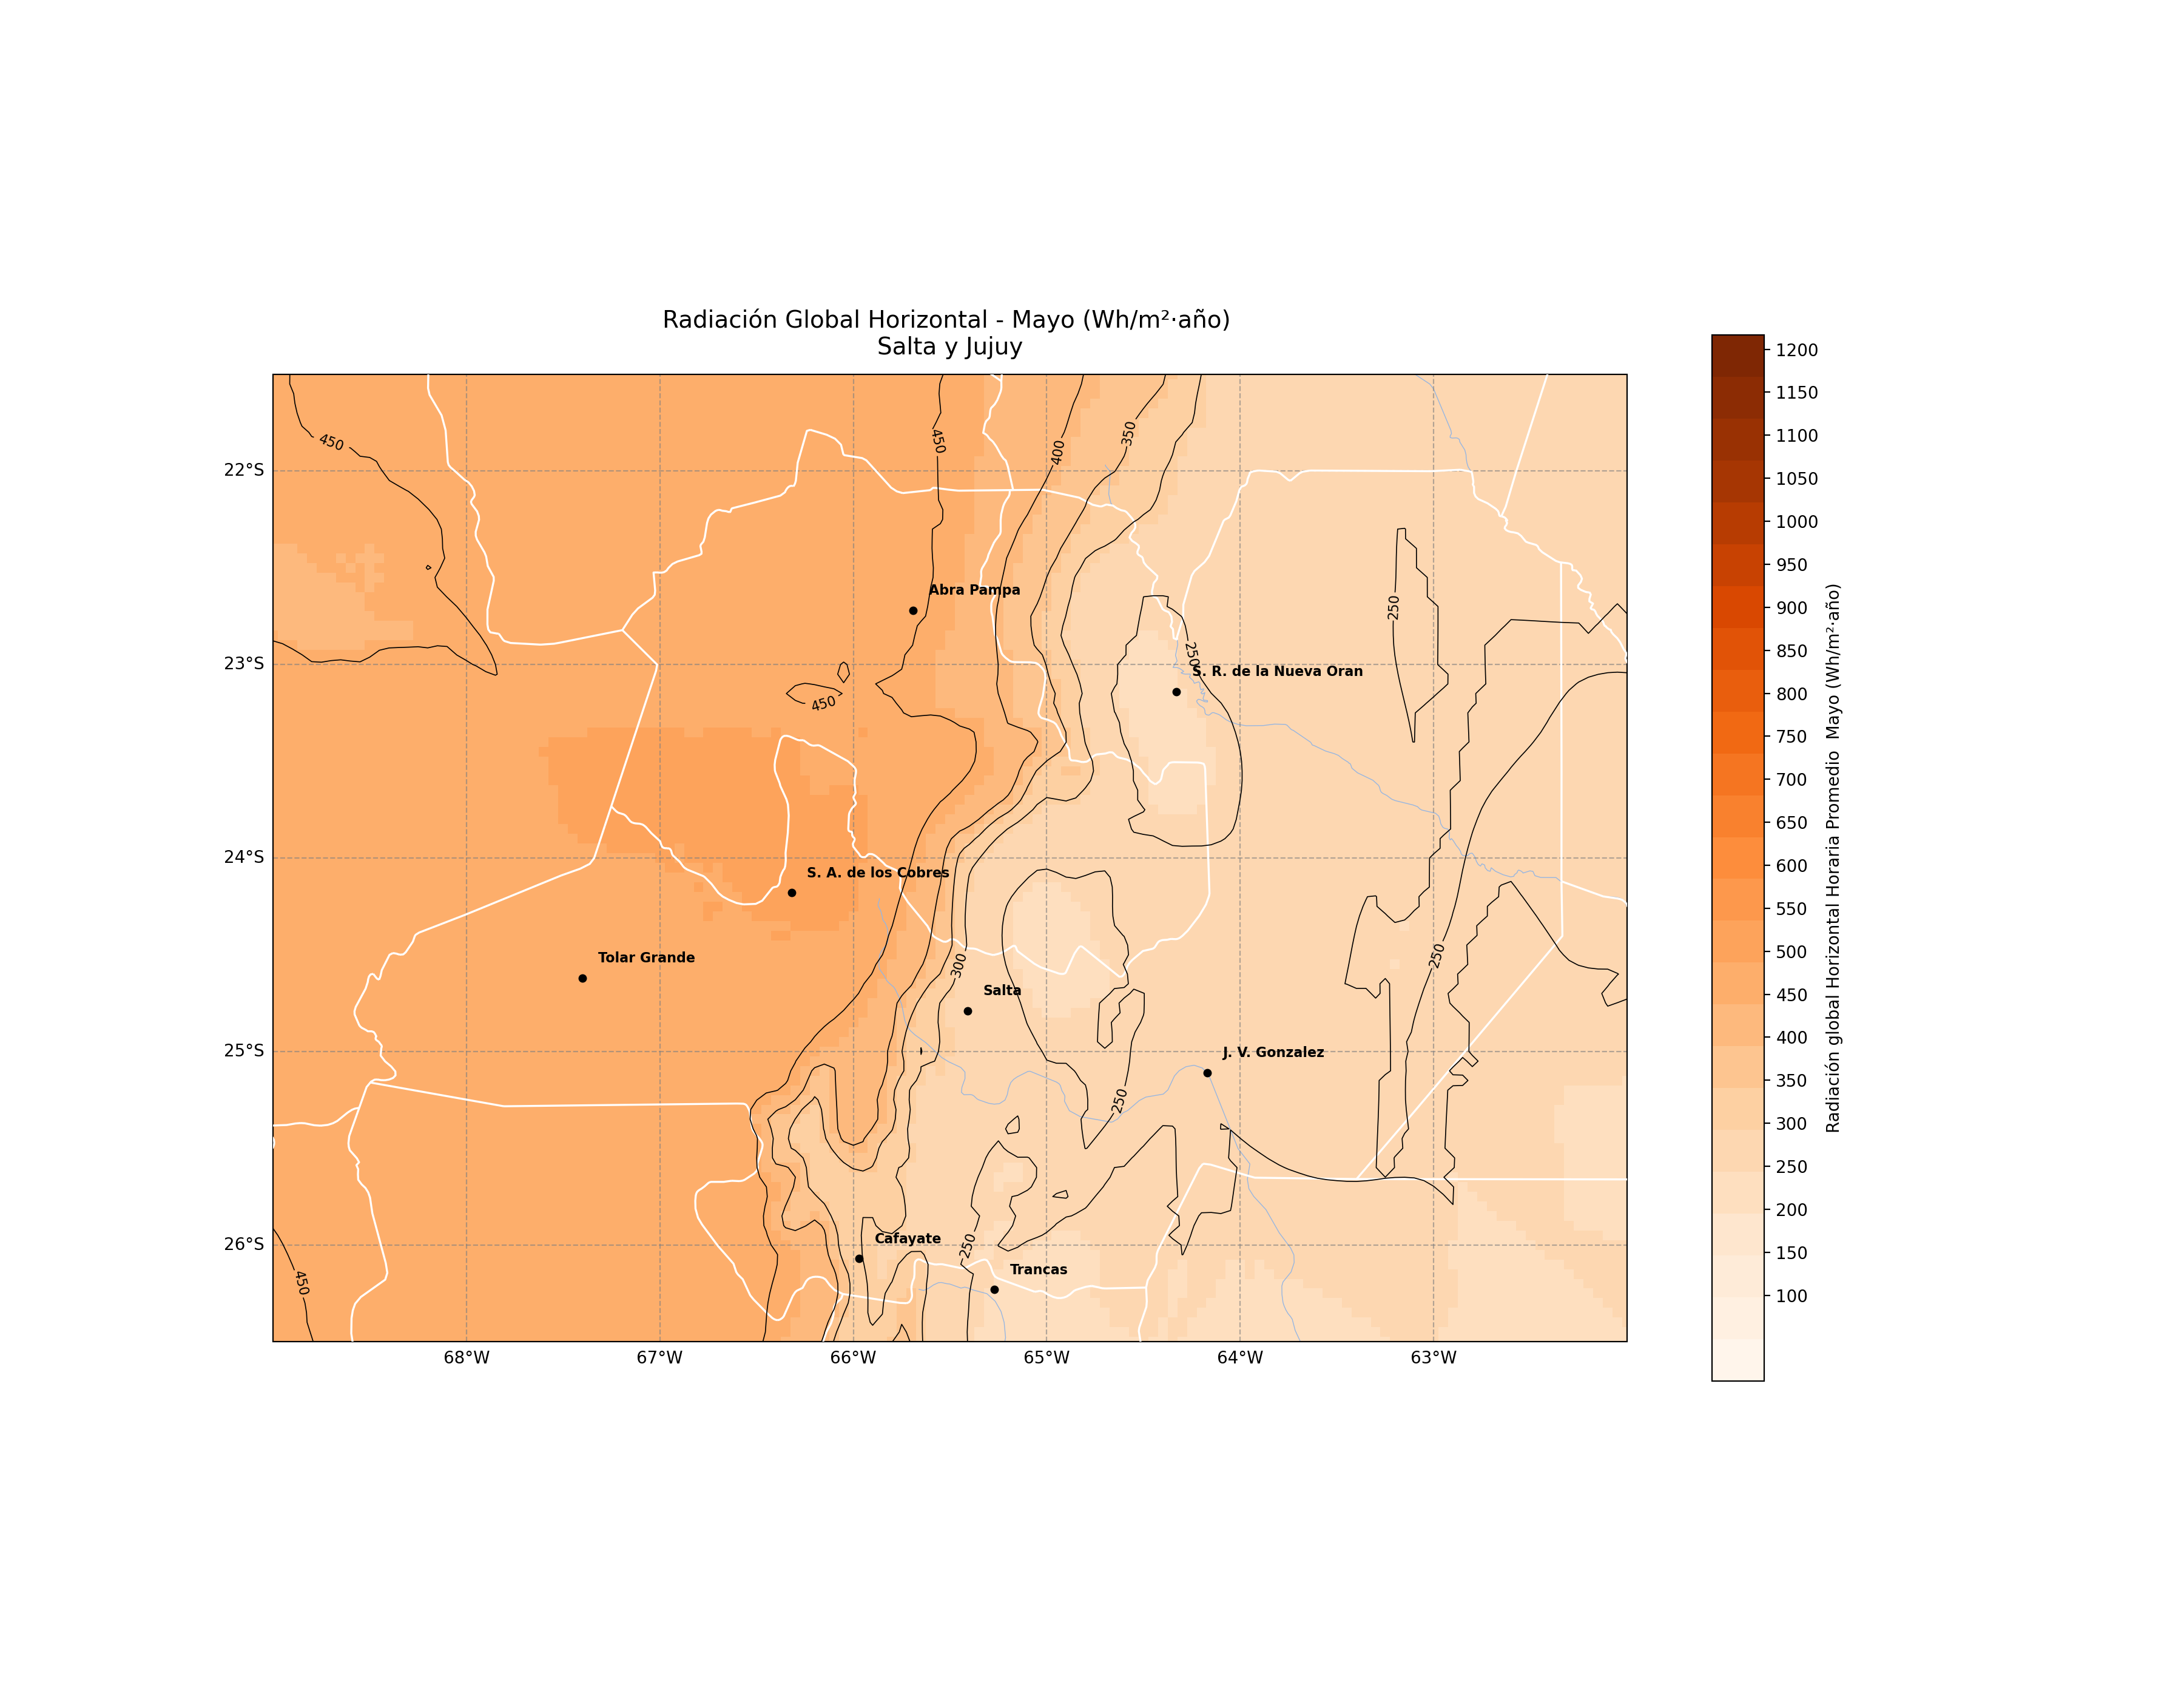
\includegraphics[width=0.95\textwidth]{figuras/Mapas/5_Mayo.png}
\caption{Mapa de GHI medio mensual – Mayo (TMY).}
\end{figure}

\begin{figure}[H]
\centering
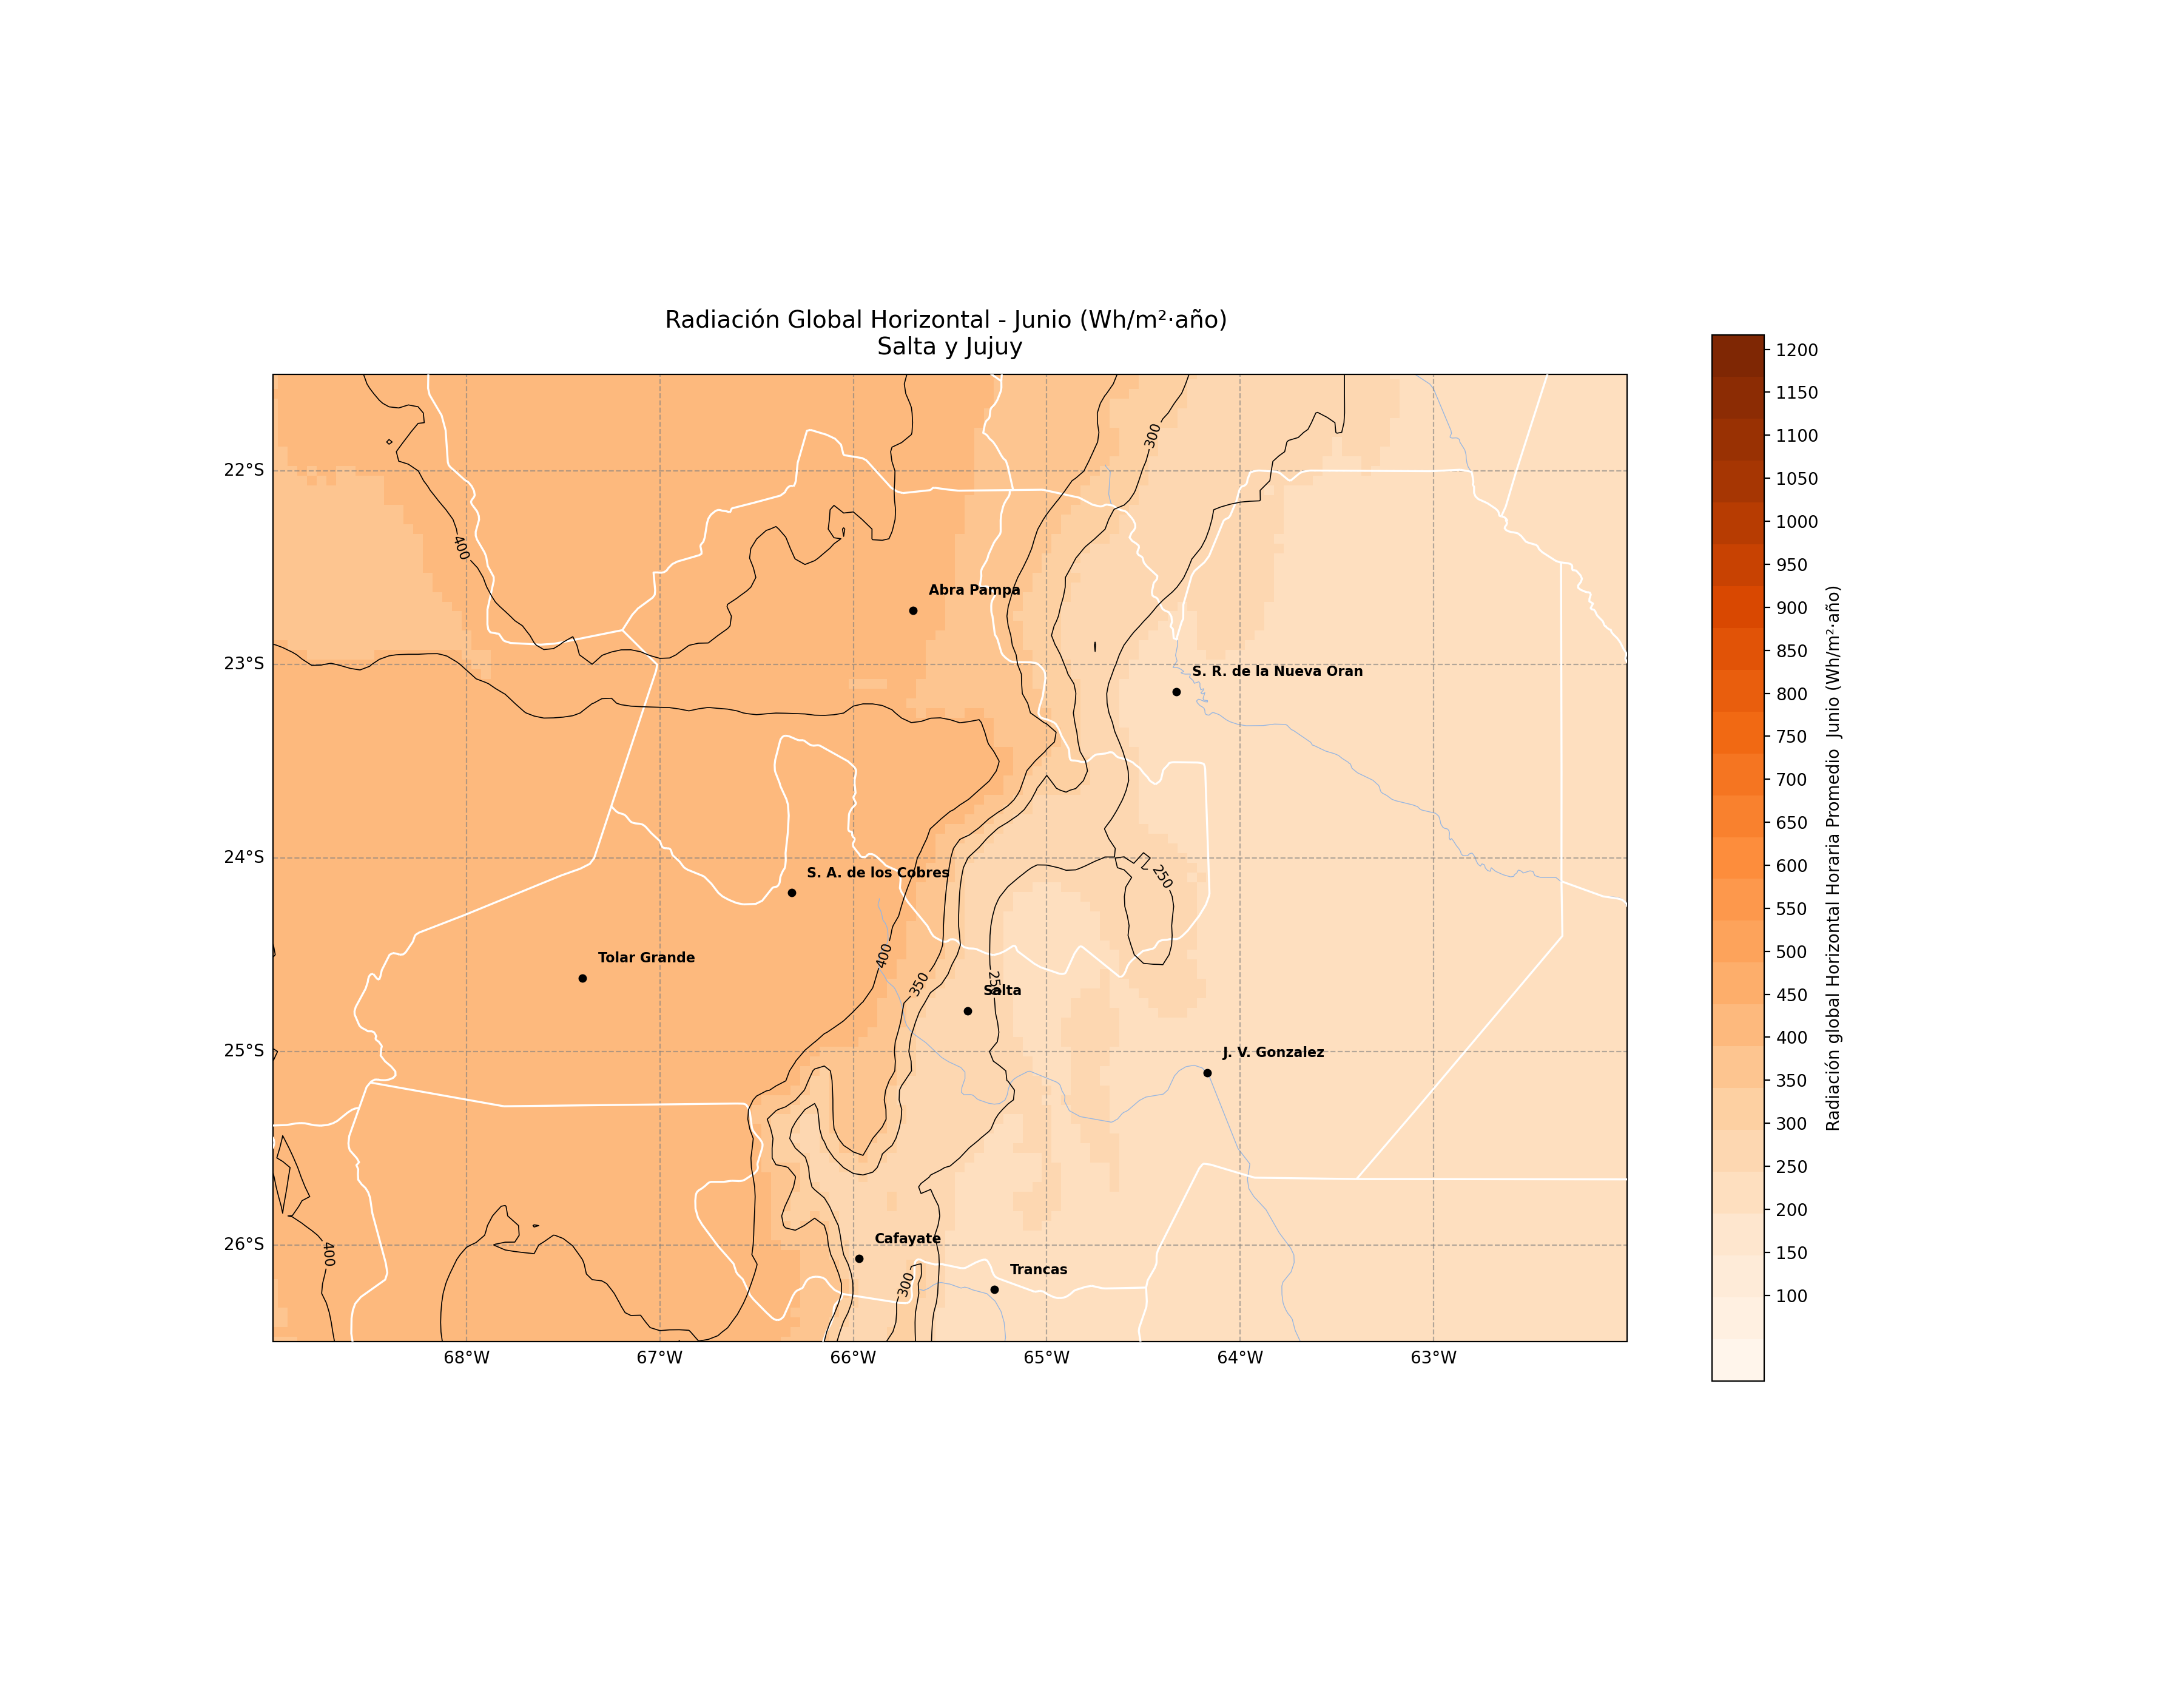
\includegraphics[width=0.95\textwidth]{figuras/Mapas/6_Junio.png}
\caption{Mapa de GHI medio mensual – Junio (TMY).}
\end{figure}

\begin{figure}[H]
\centering
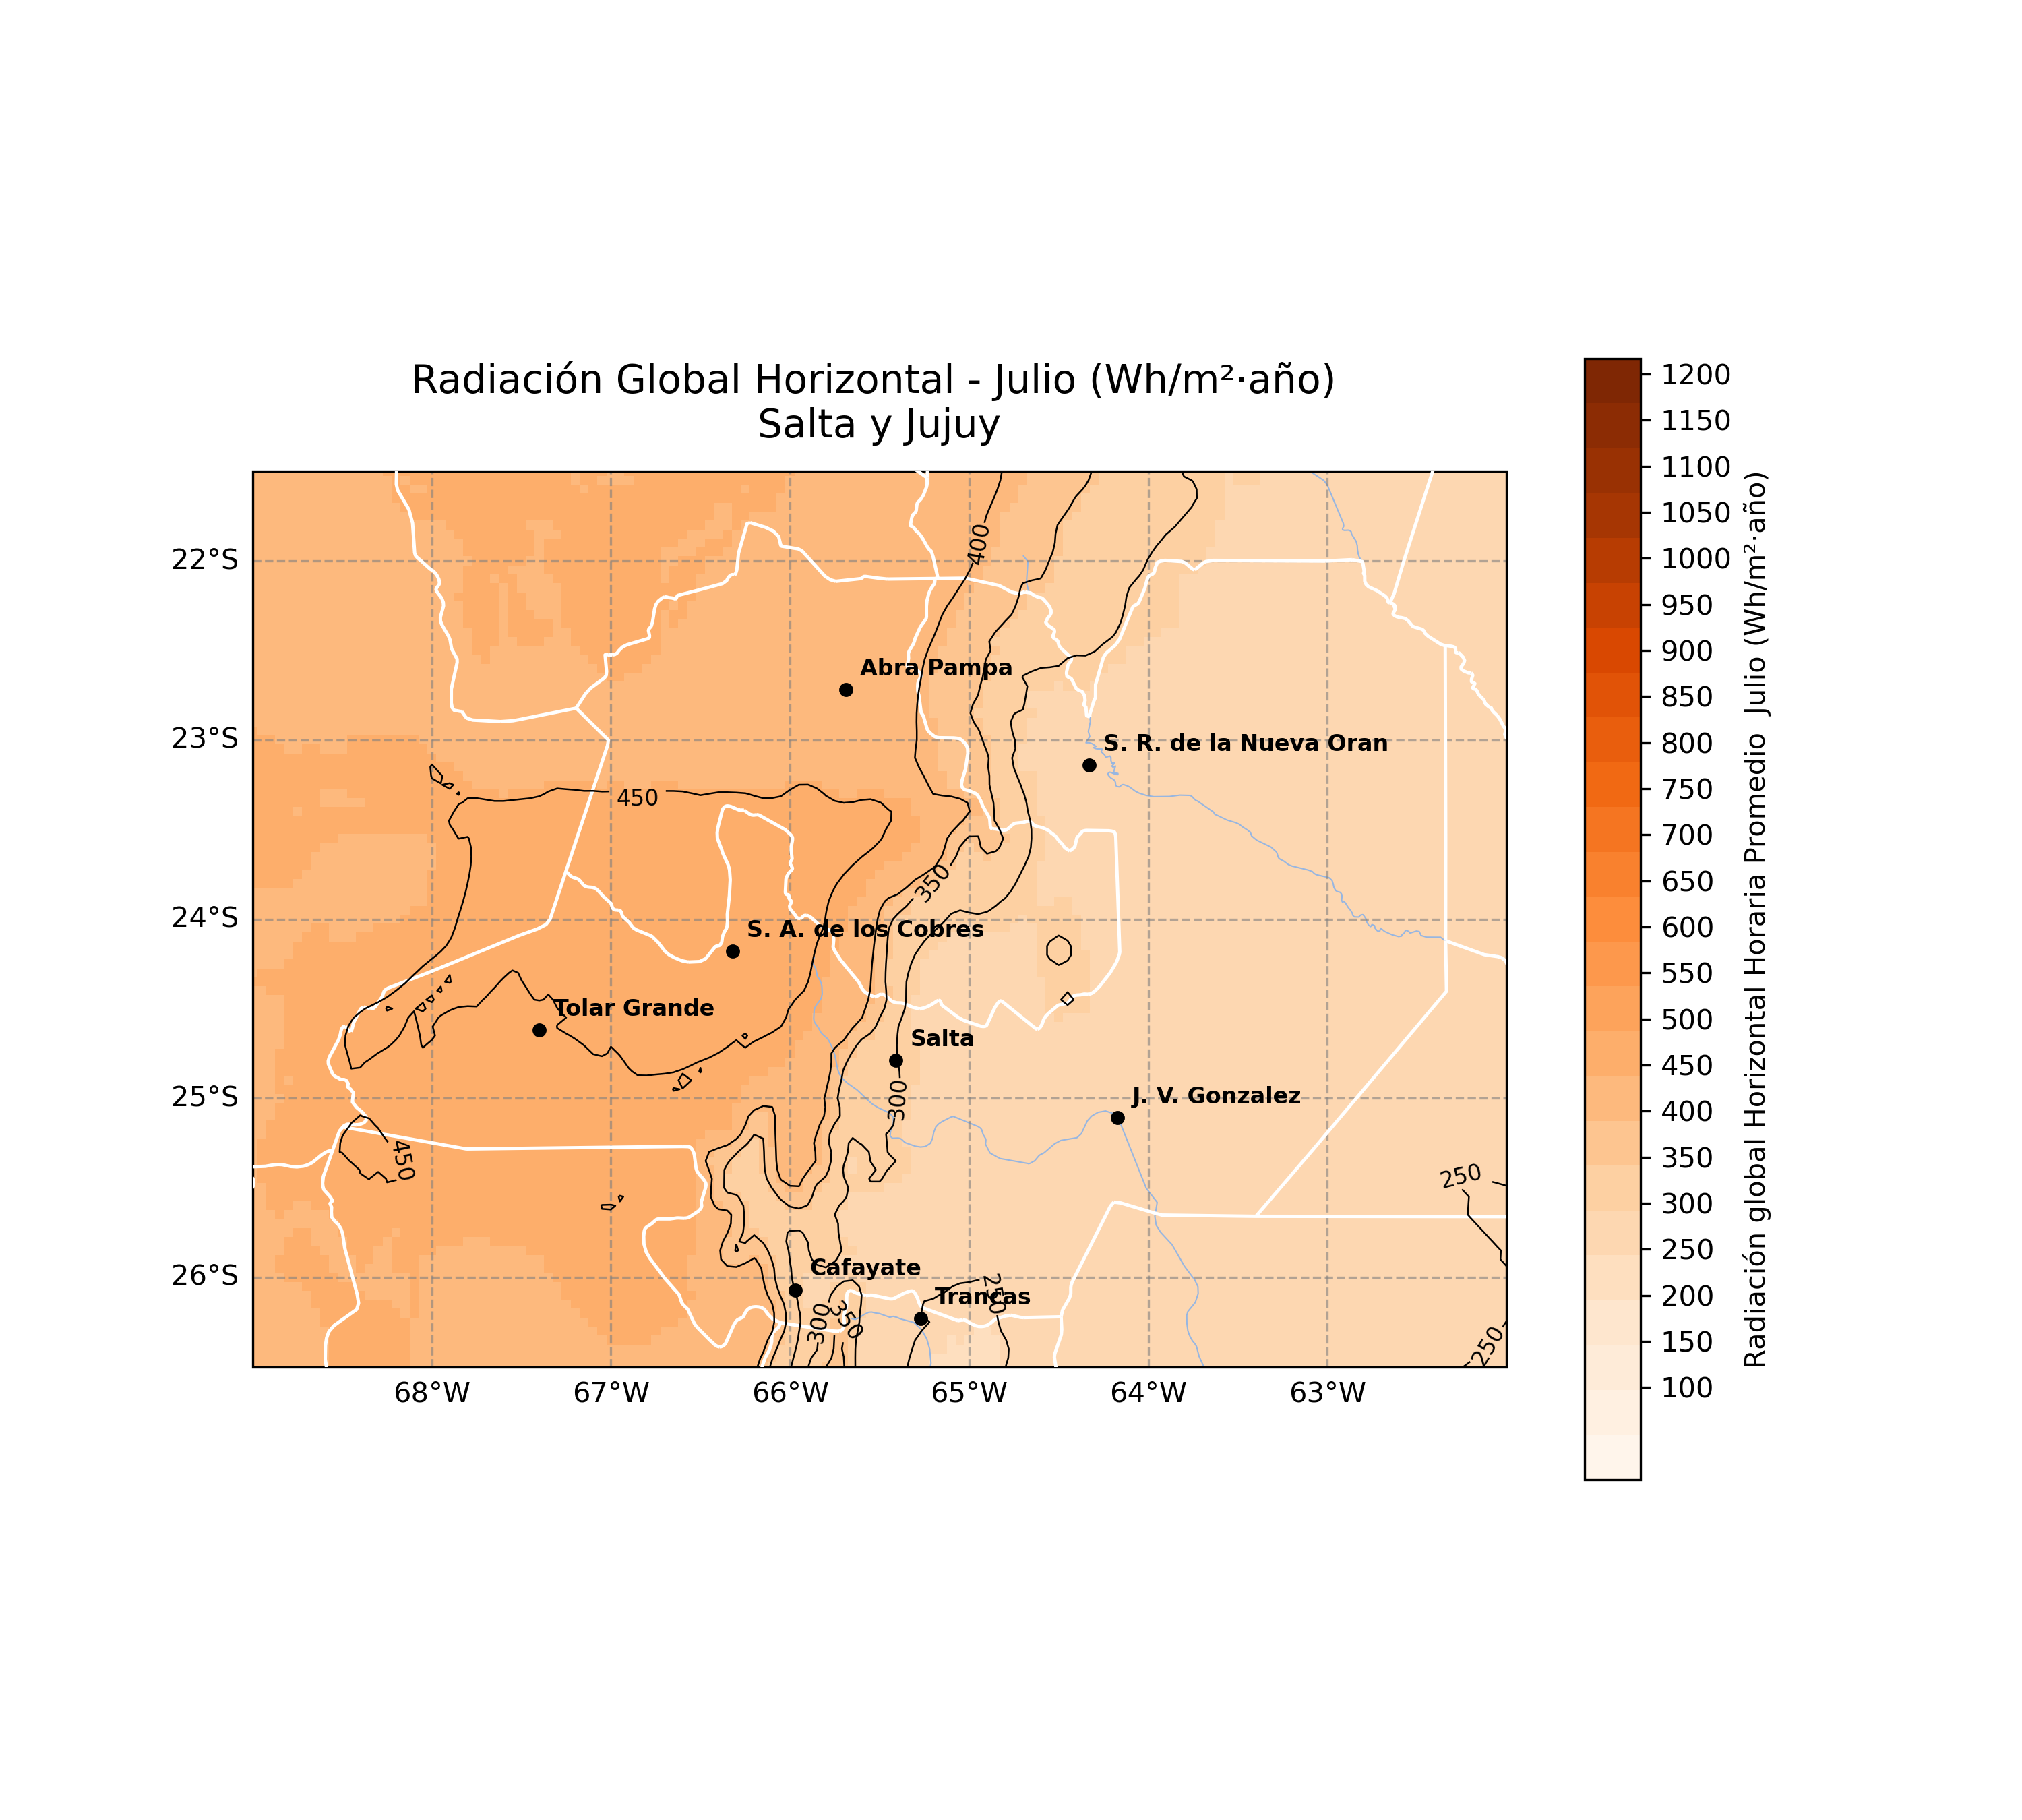
\includegraphics[width=0.95\textwidth]{figuras/Mapas/7_Julio.png}
\caption{Mapa de GHI medio mensual – Julio (TMY).}
\end{figure}

\begin{figure}[H]
\centering
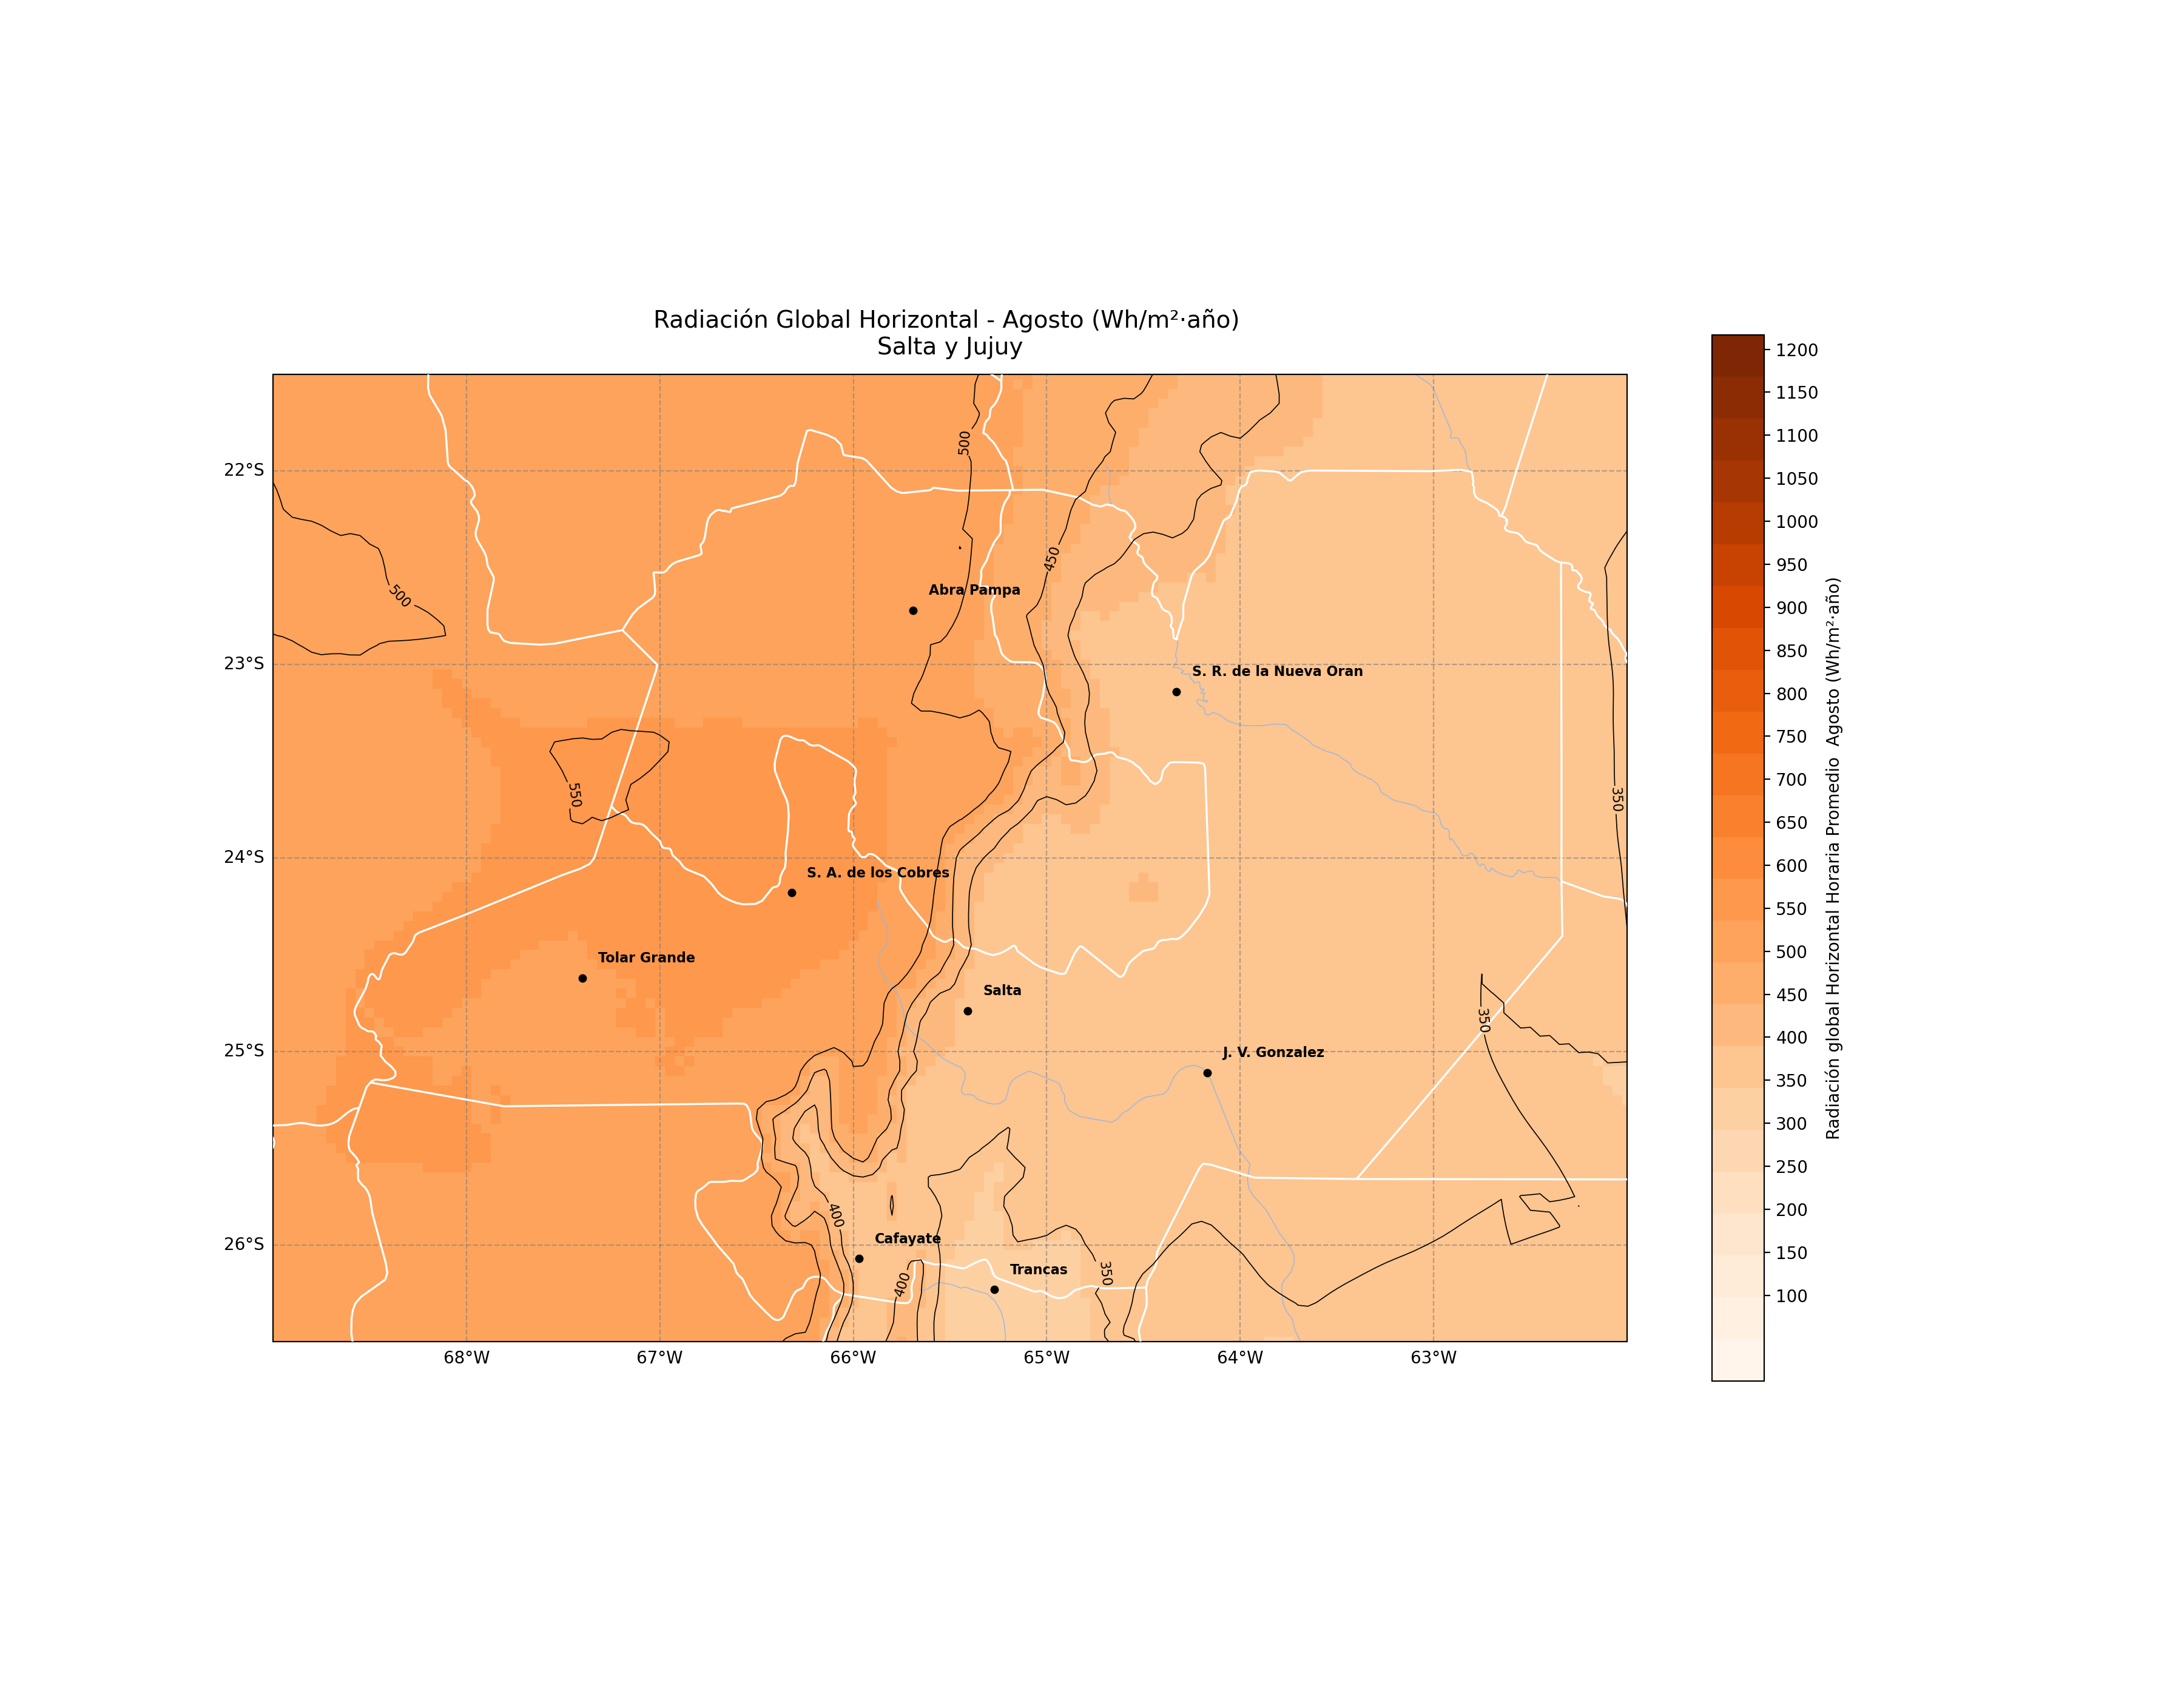
\includegraphics[width=0.95\textwidth]{figuras/Mapas/8_Agosto.png}
\caption{Mapa de GHI medio mensual – Agosto (TMY).}
\end{figure}

\begin{figure}[H]
\centering
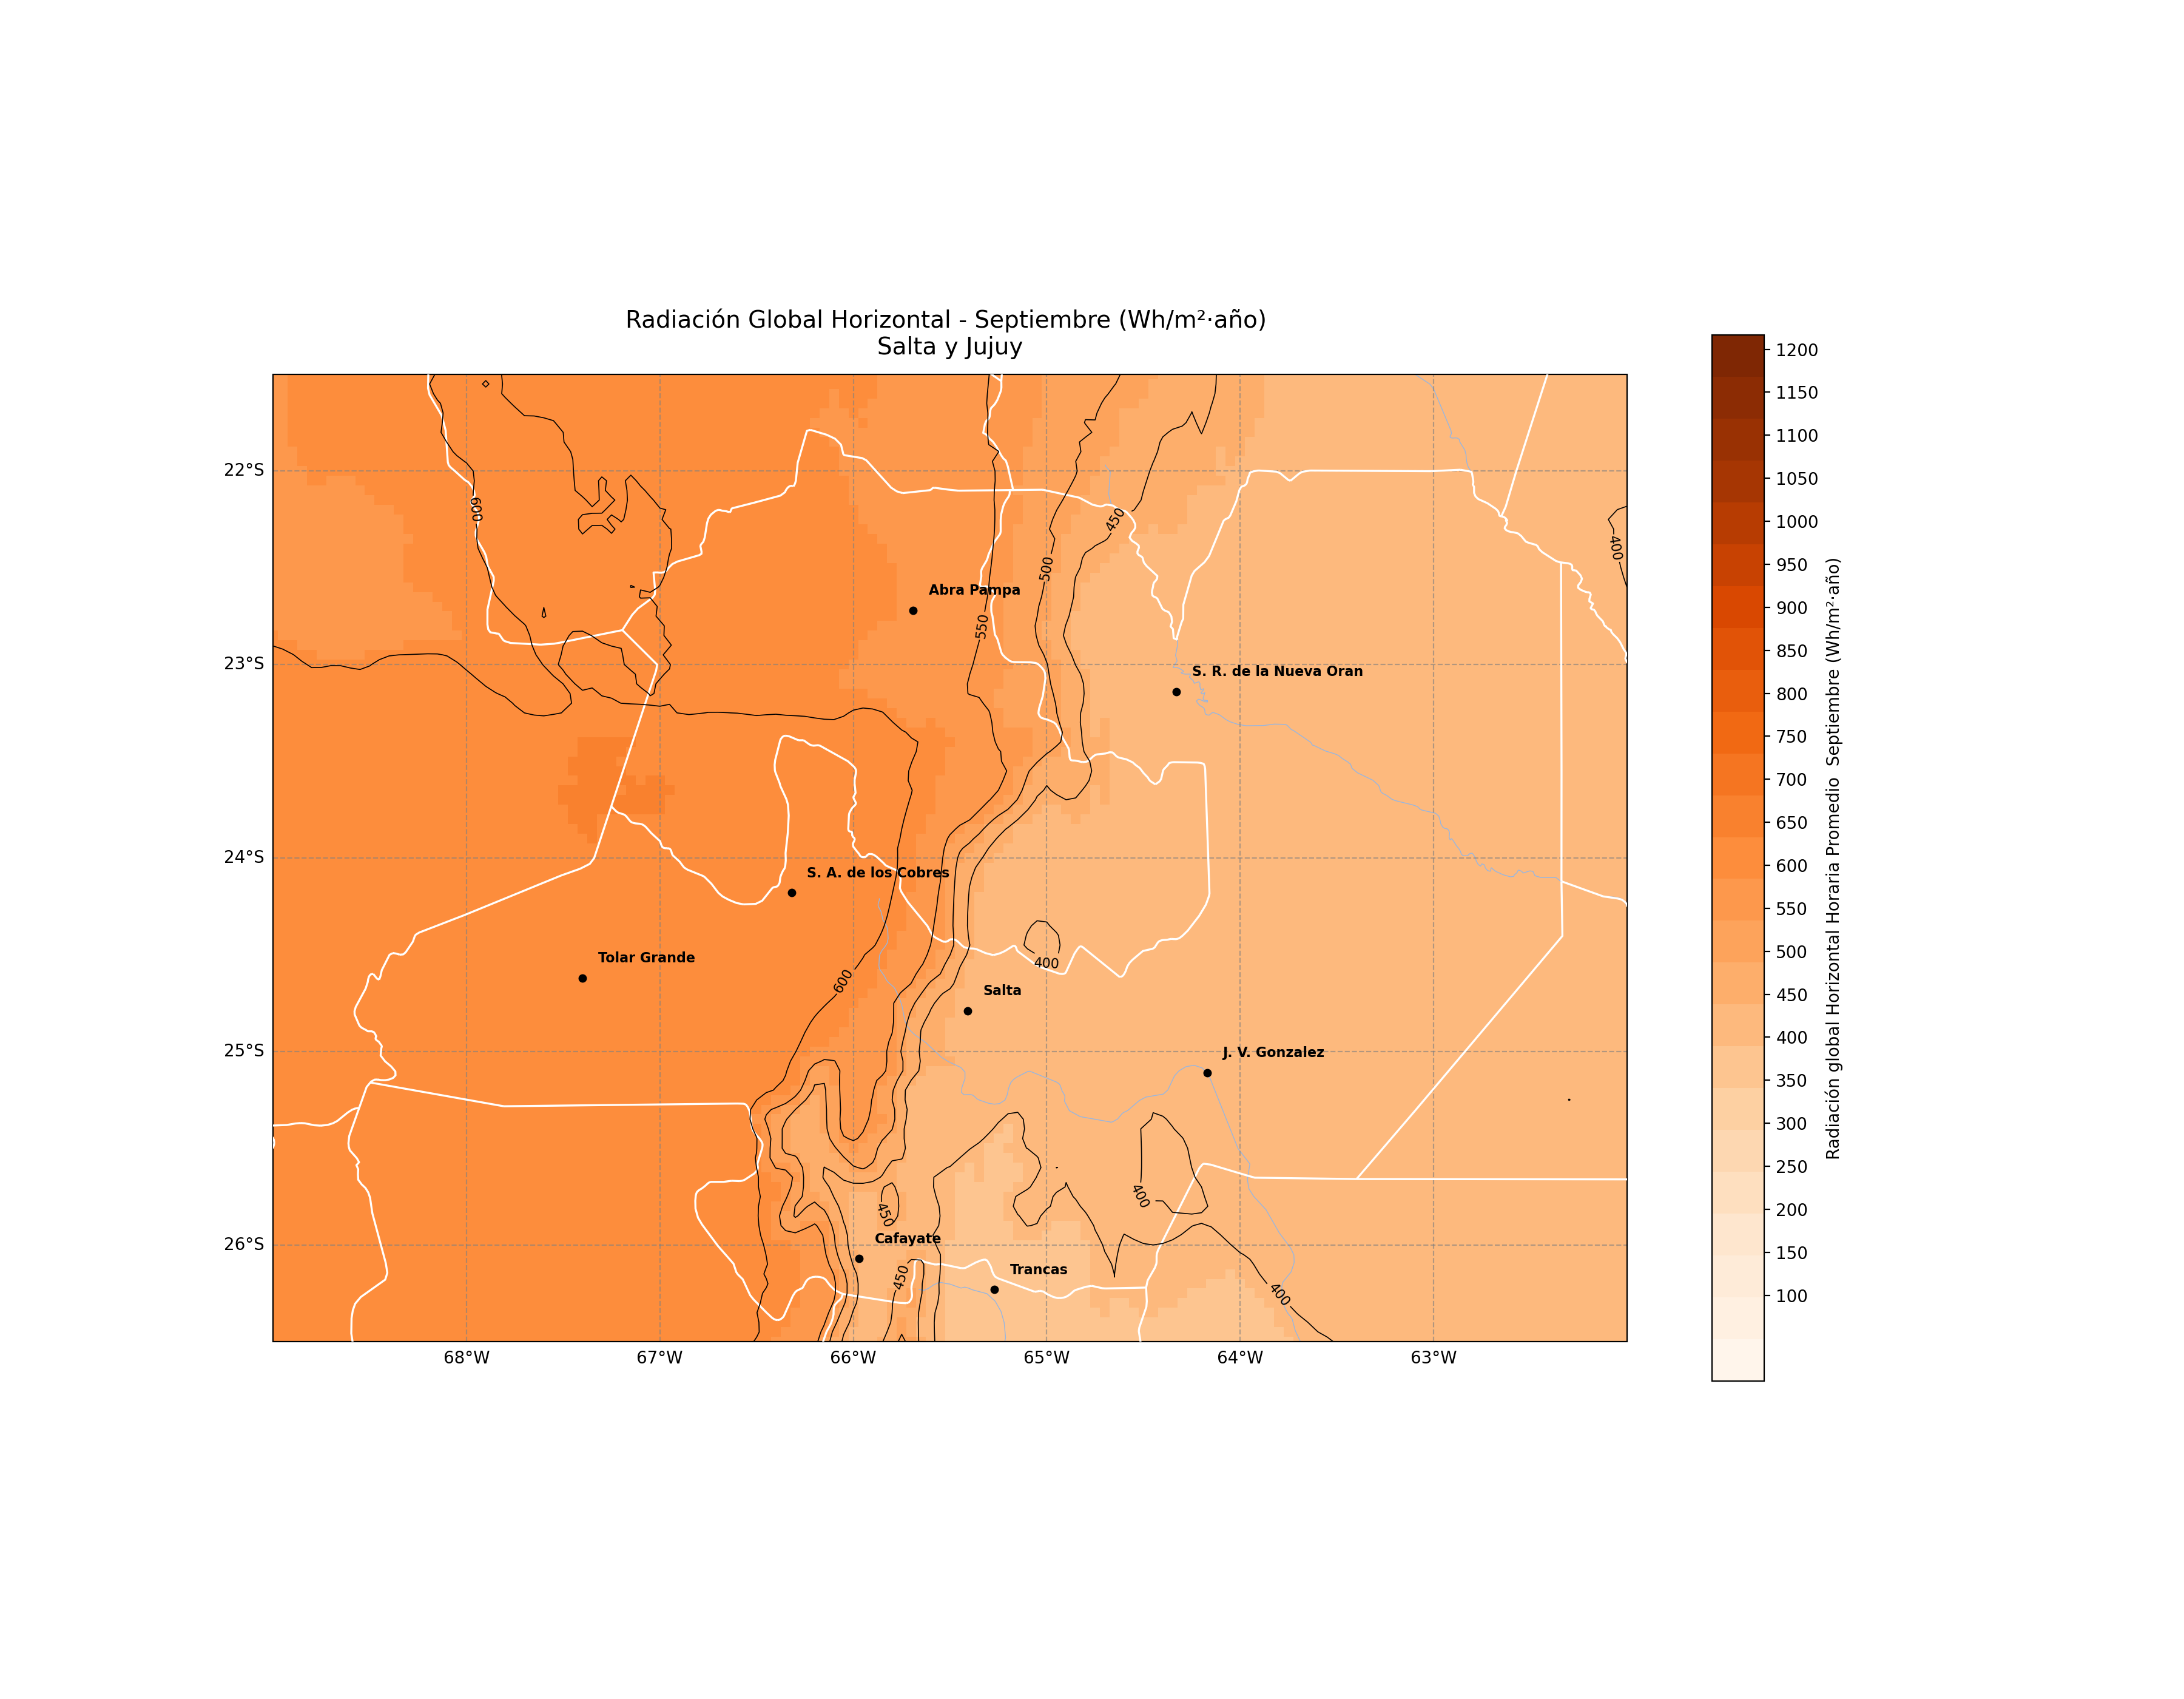
\includegraphics[width=0.95\textwidth]{figuras/Mapas/9_Septiembre.png}
\caption{Mapa de GHI medio mensual – Septiembre (TMY).}
\end{figure}

\begin{figure}[H]
\centering
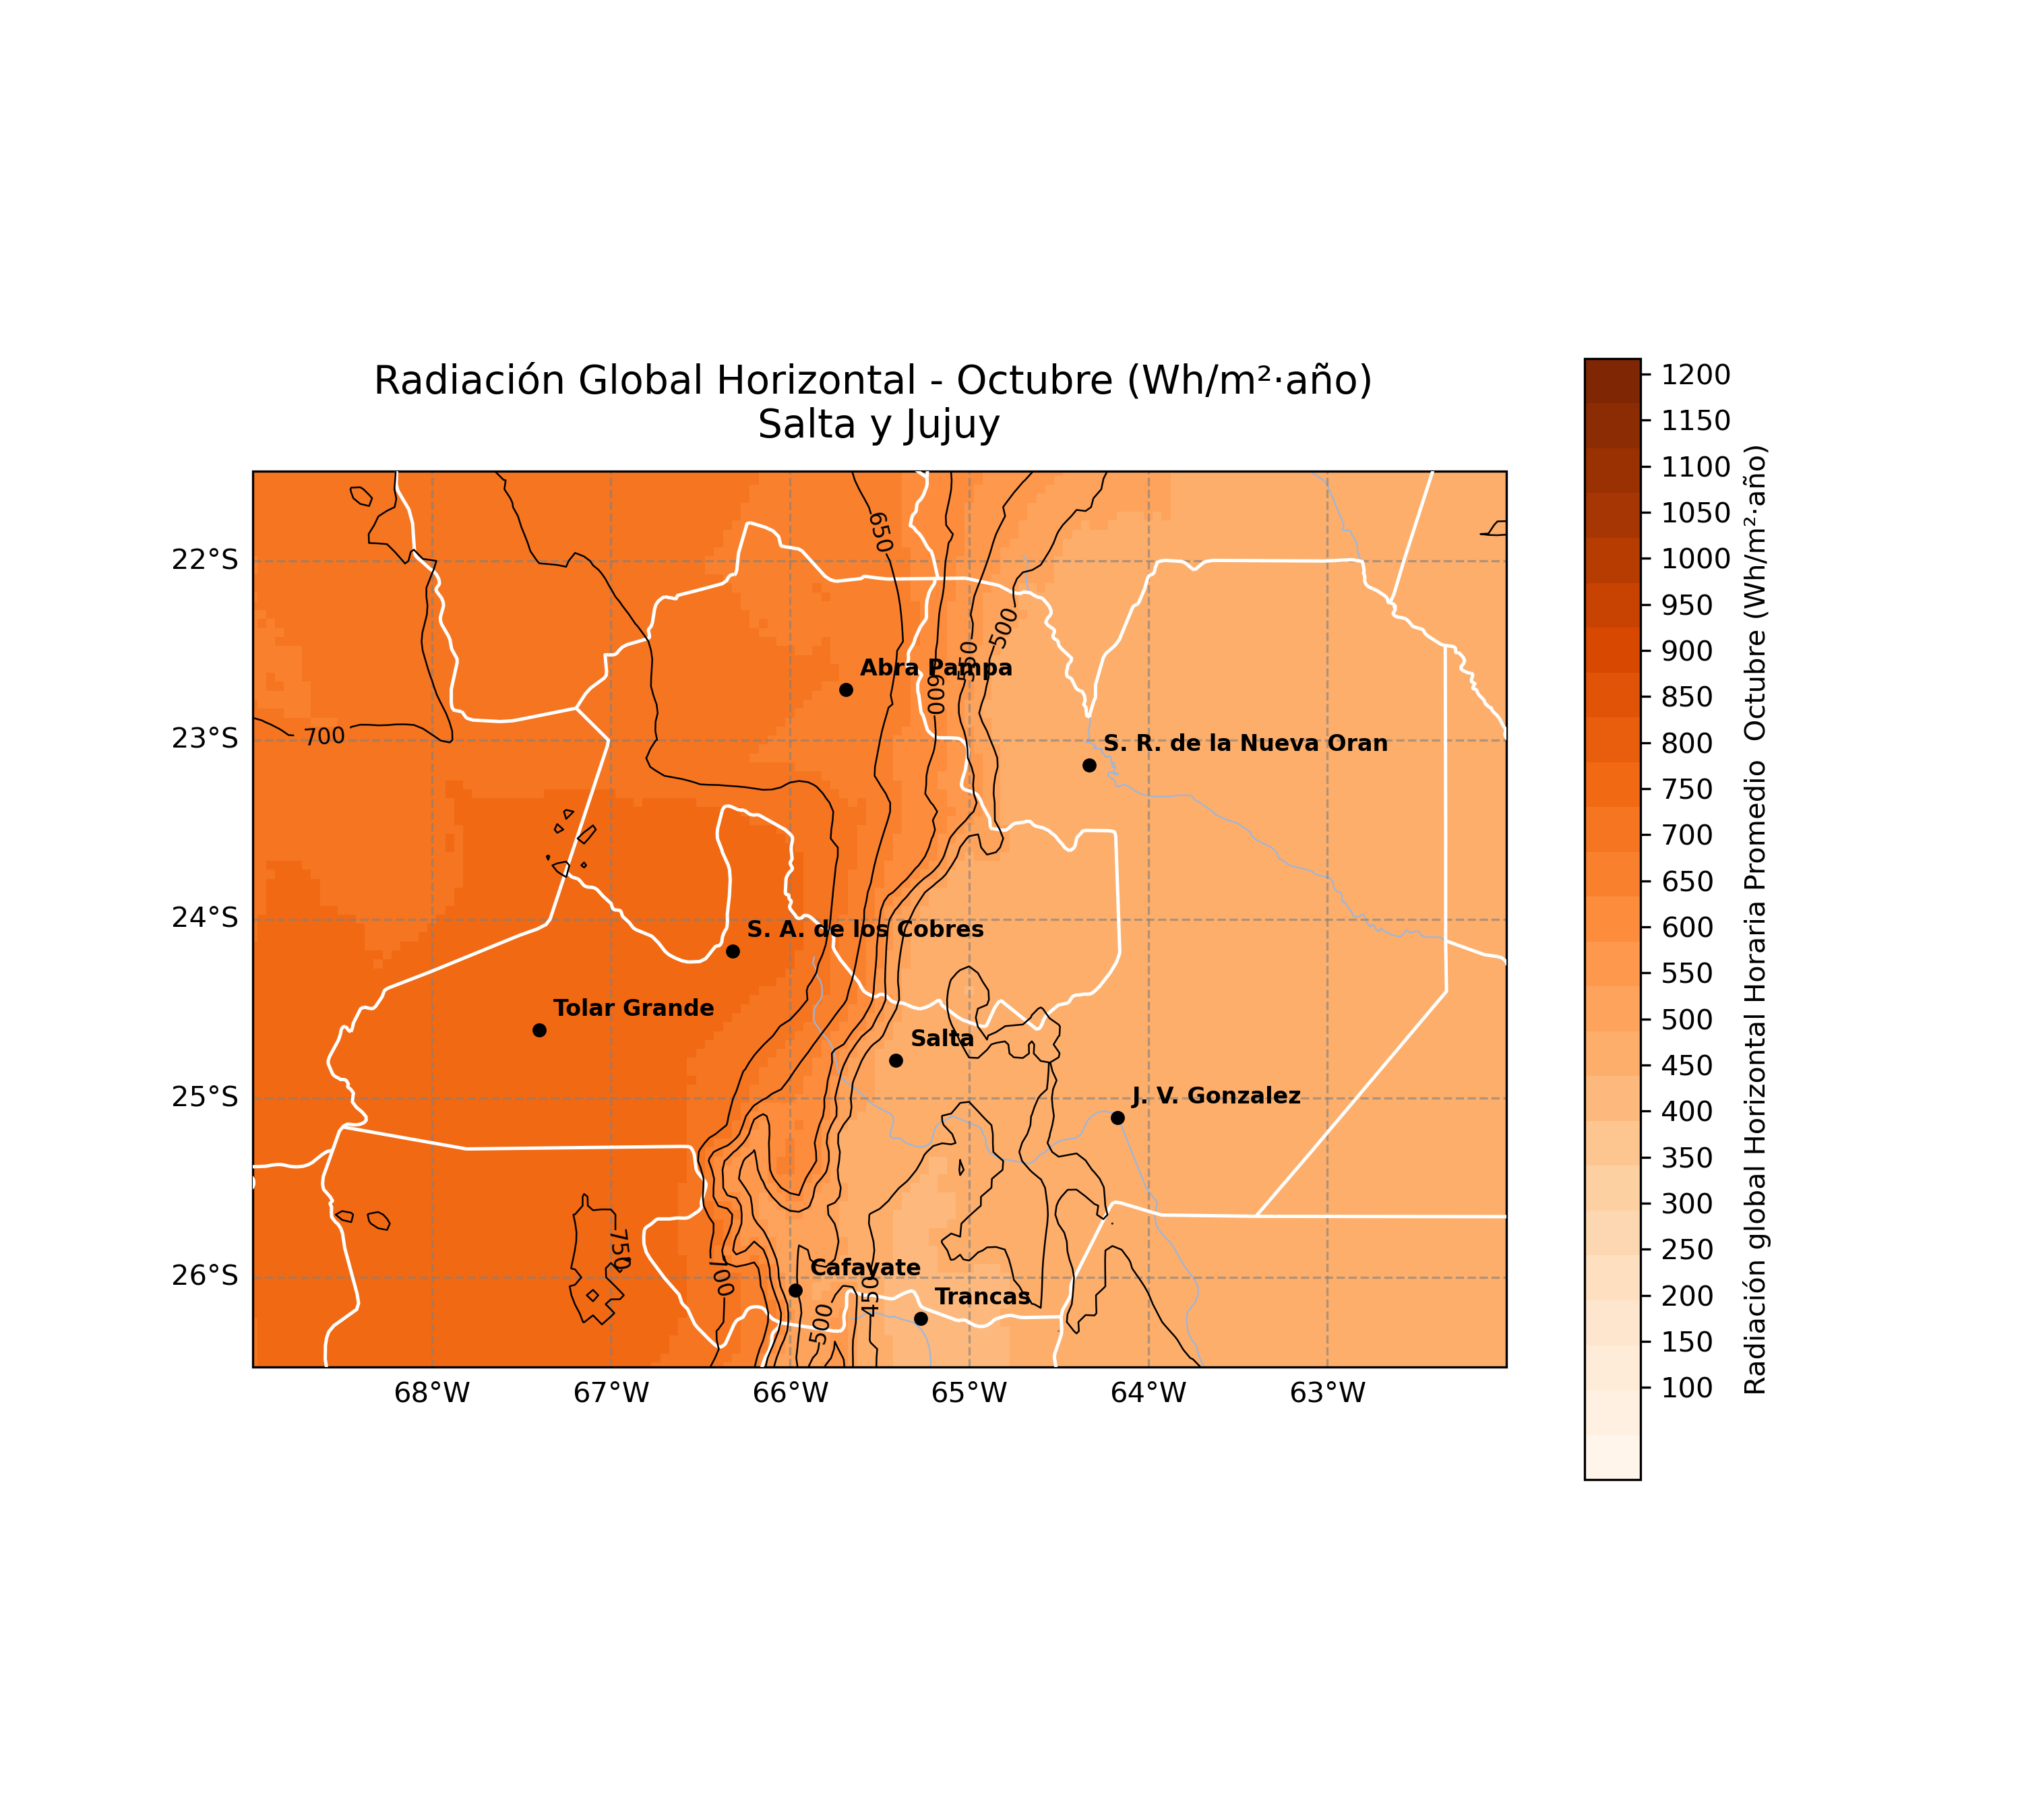
\includegraphics[width=0.95\textwidth]{figuras/Mapas/10_Octubre.png}
\caption{Mapa de GHI medio mensual – Octubre (TMY).}
\end{figure}

\begin{figure}[H]
\centering
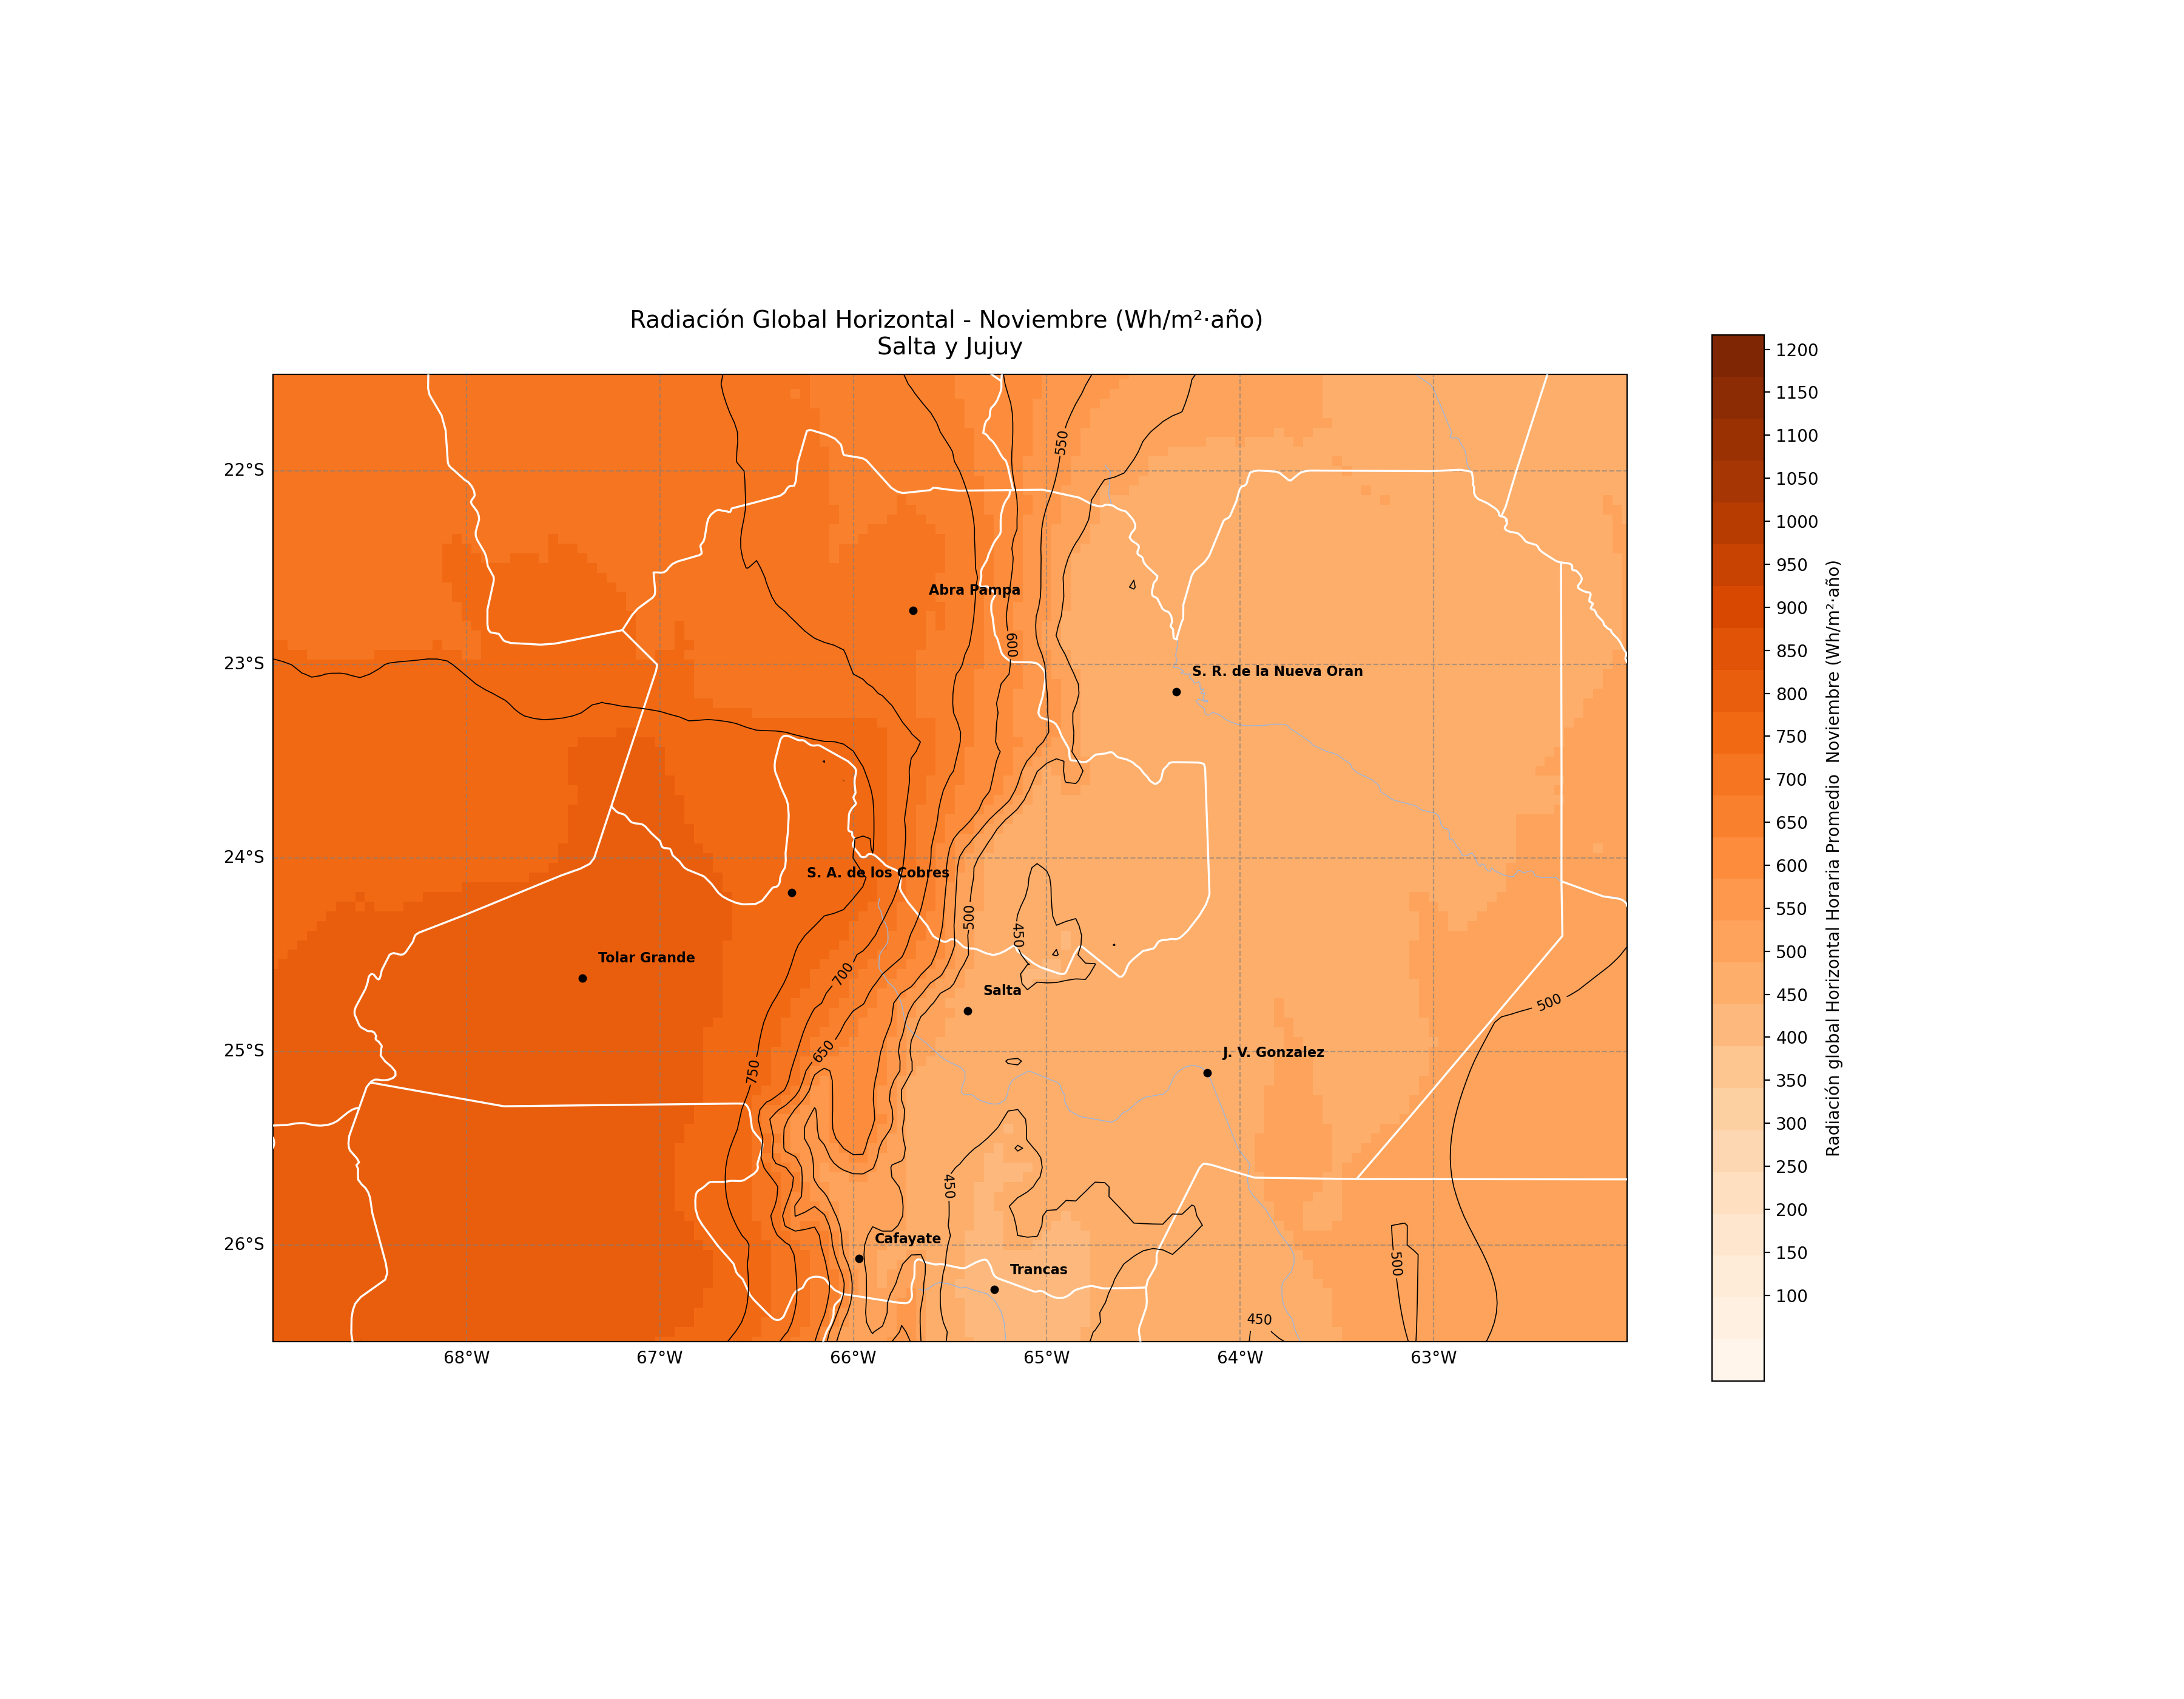
\includegraphics[width=0.95\textwidth]{figuras/Mapas/11_Noviembre.png}
\caption{Mapa de GHI medio mensual – Noviembre (TMY).}
\end{figure}

\begin{figure}[H]
\centering
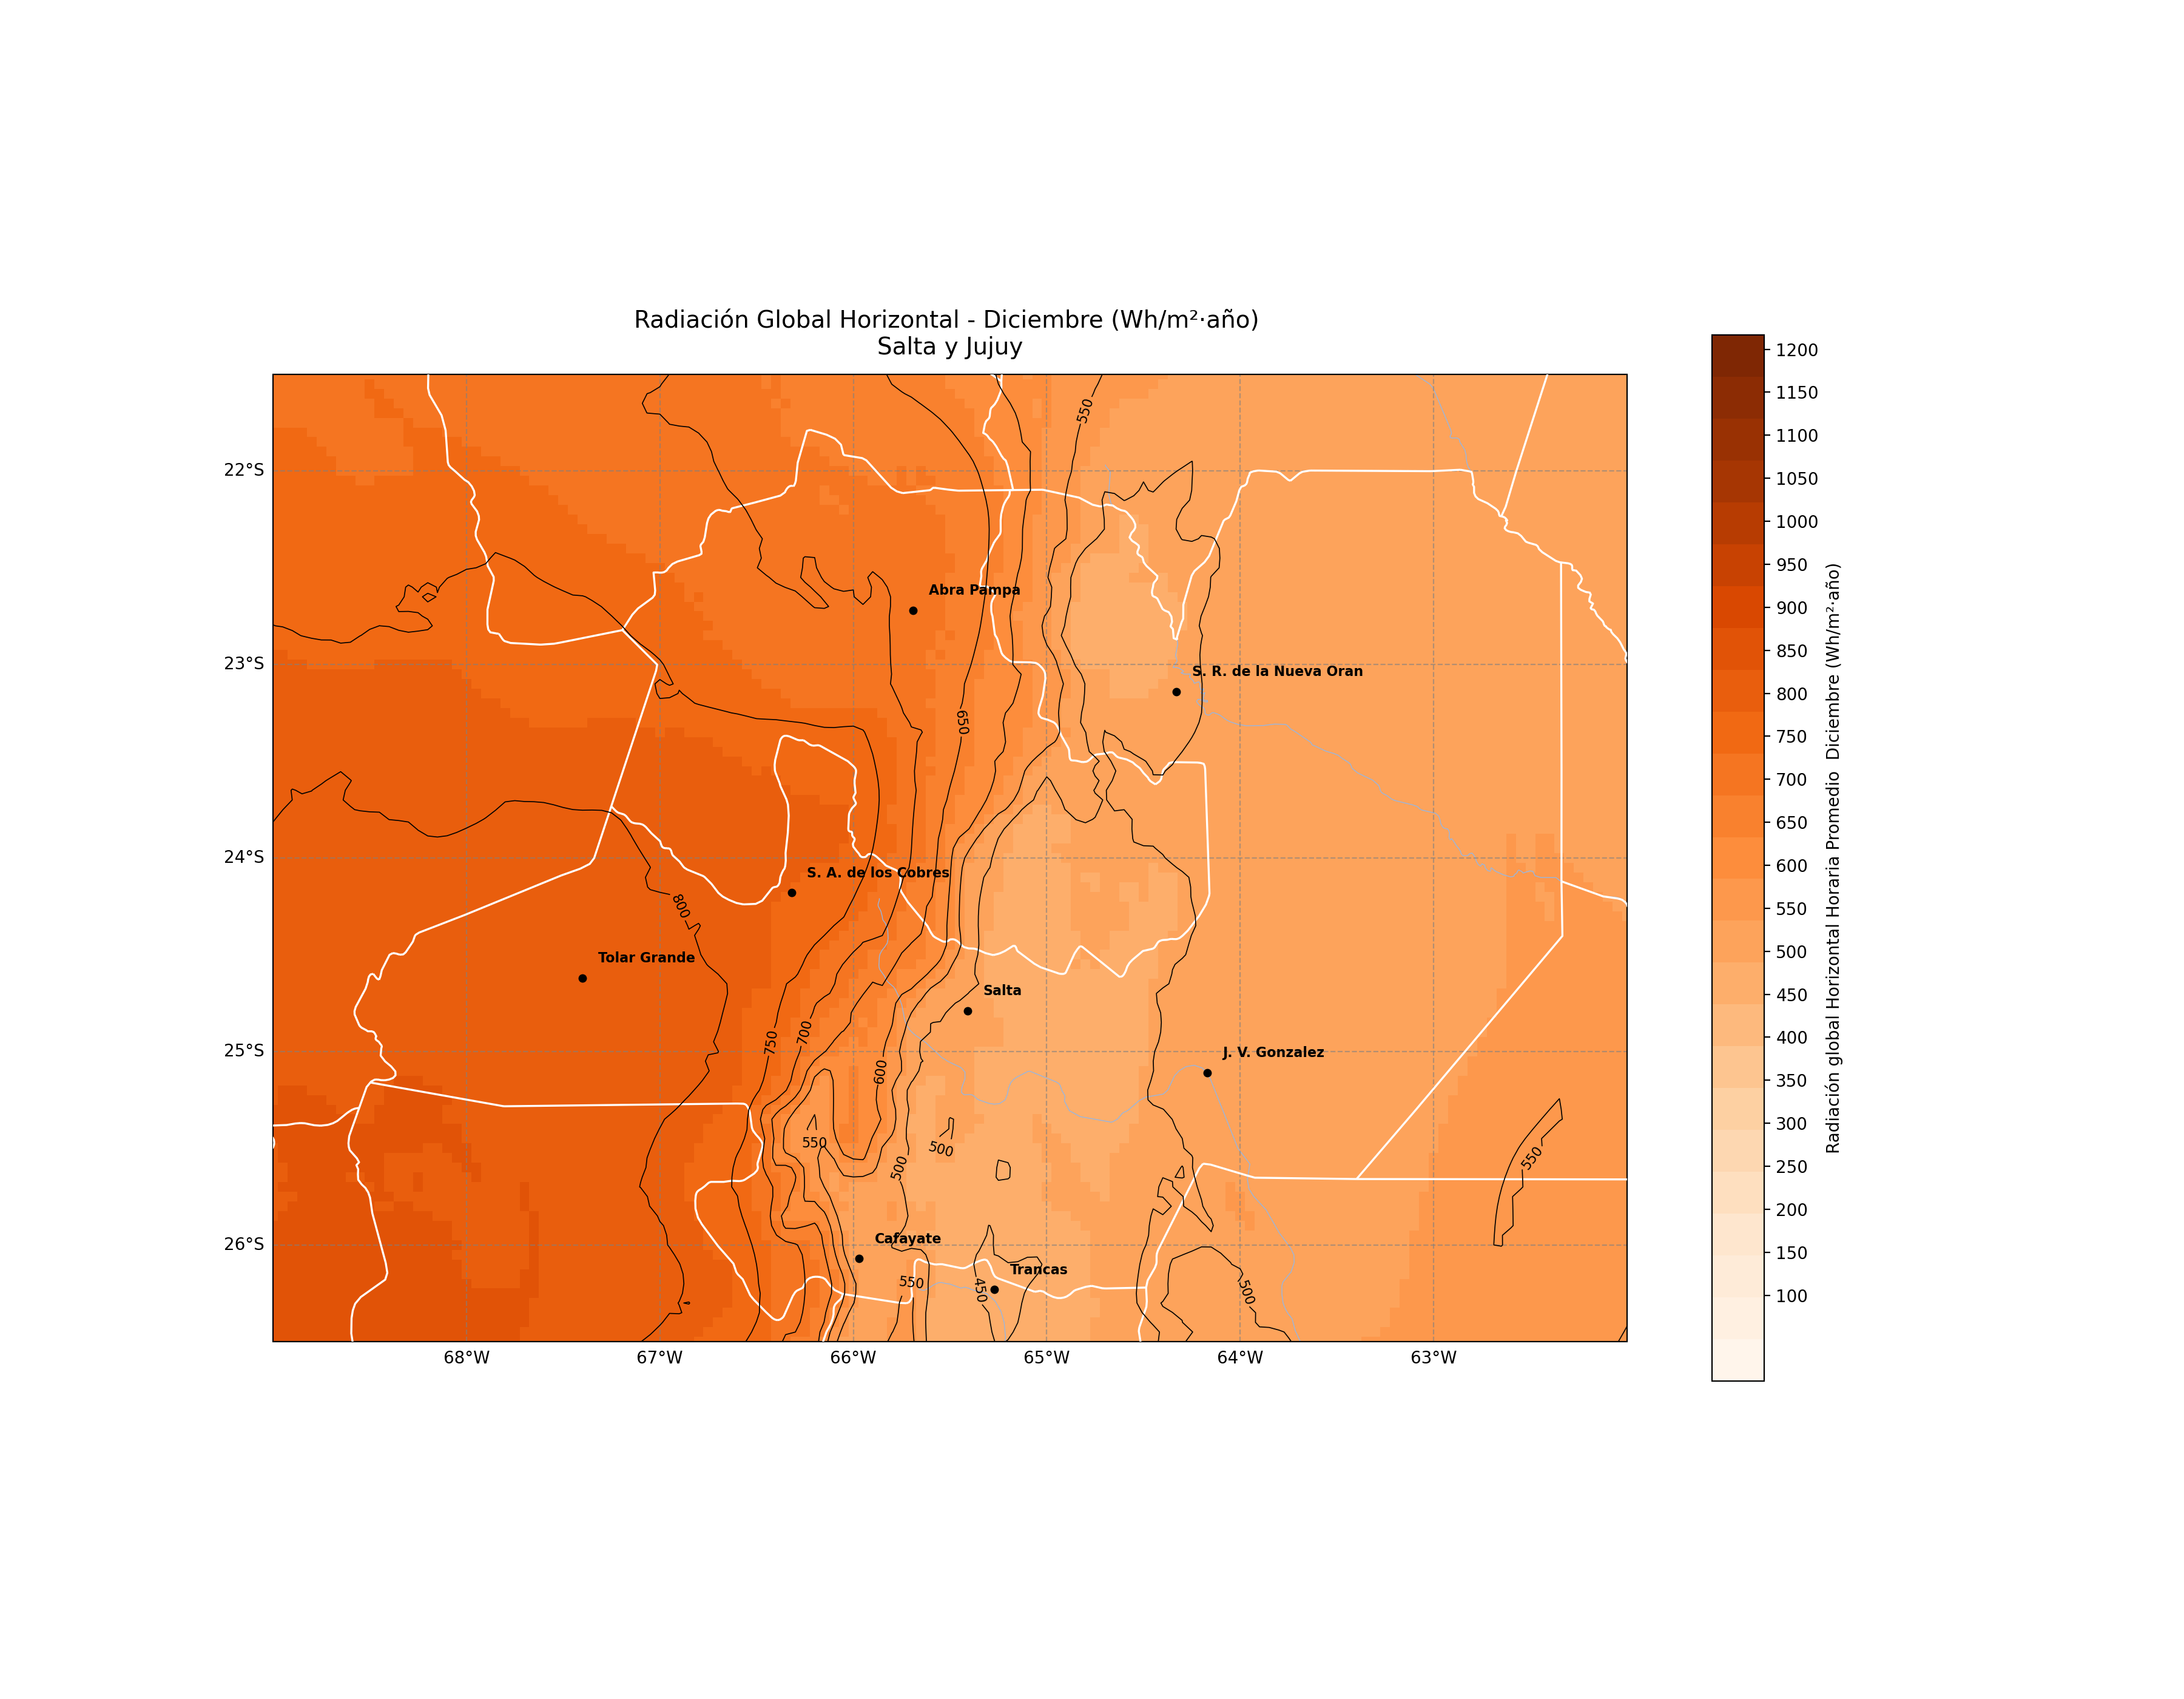
\includegraphics[width=0.95\textwidth]{figuras/Mapas/12_Diciembre.png}
\caption{Mapa de GHI medio mensual – Diciembre (TMY).}
\end{figure}




	
\begin{figure}
    \centering	
        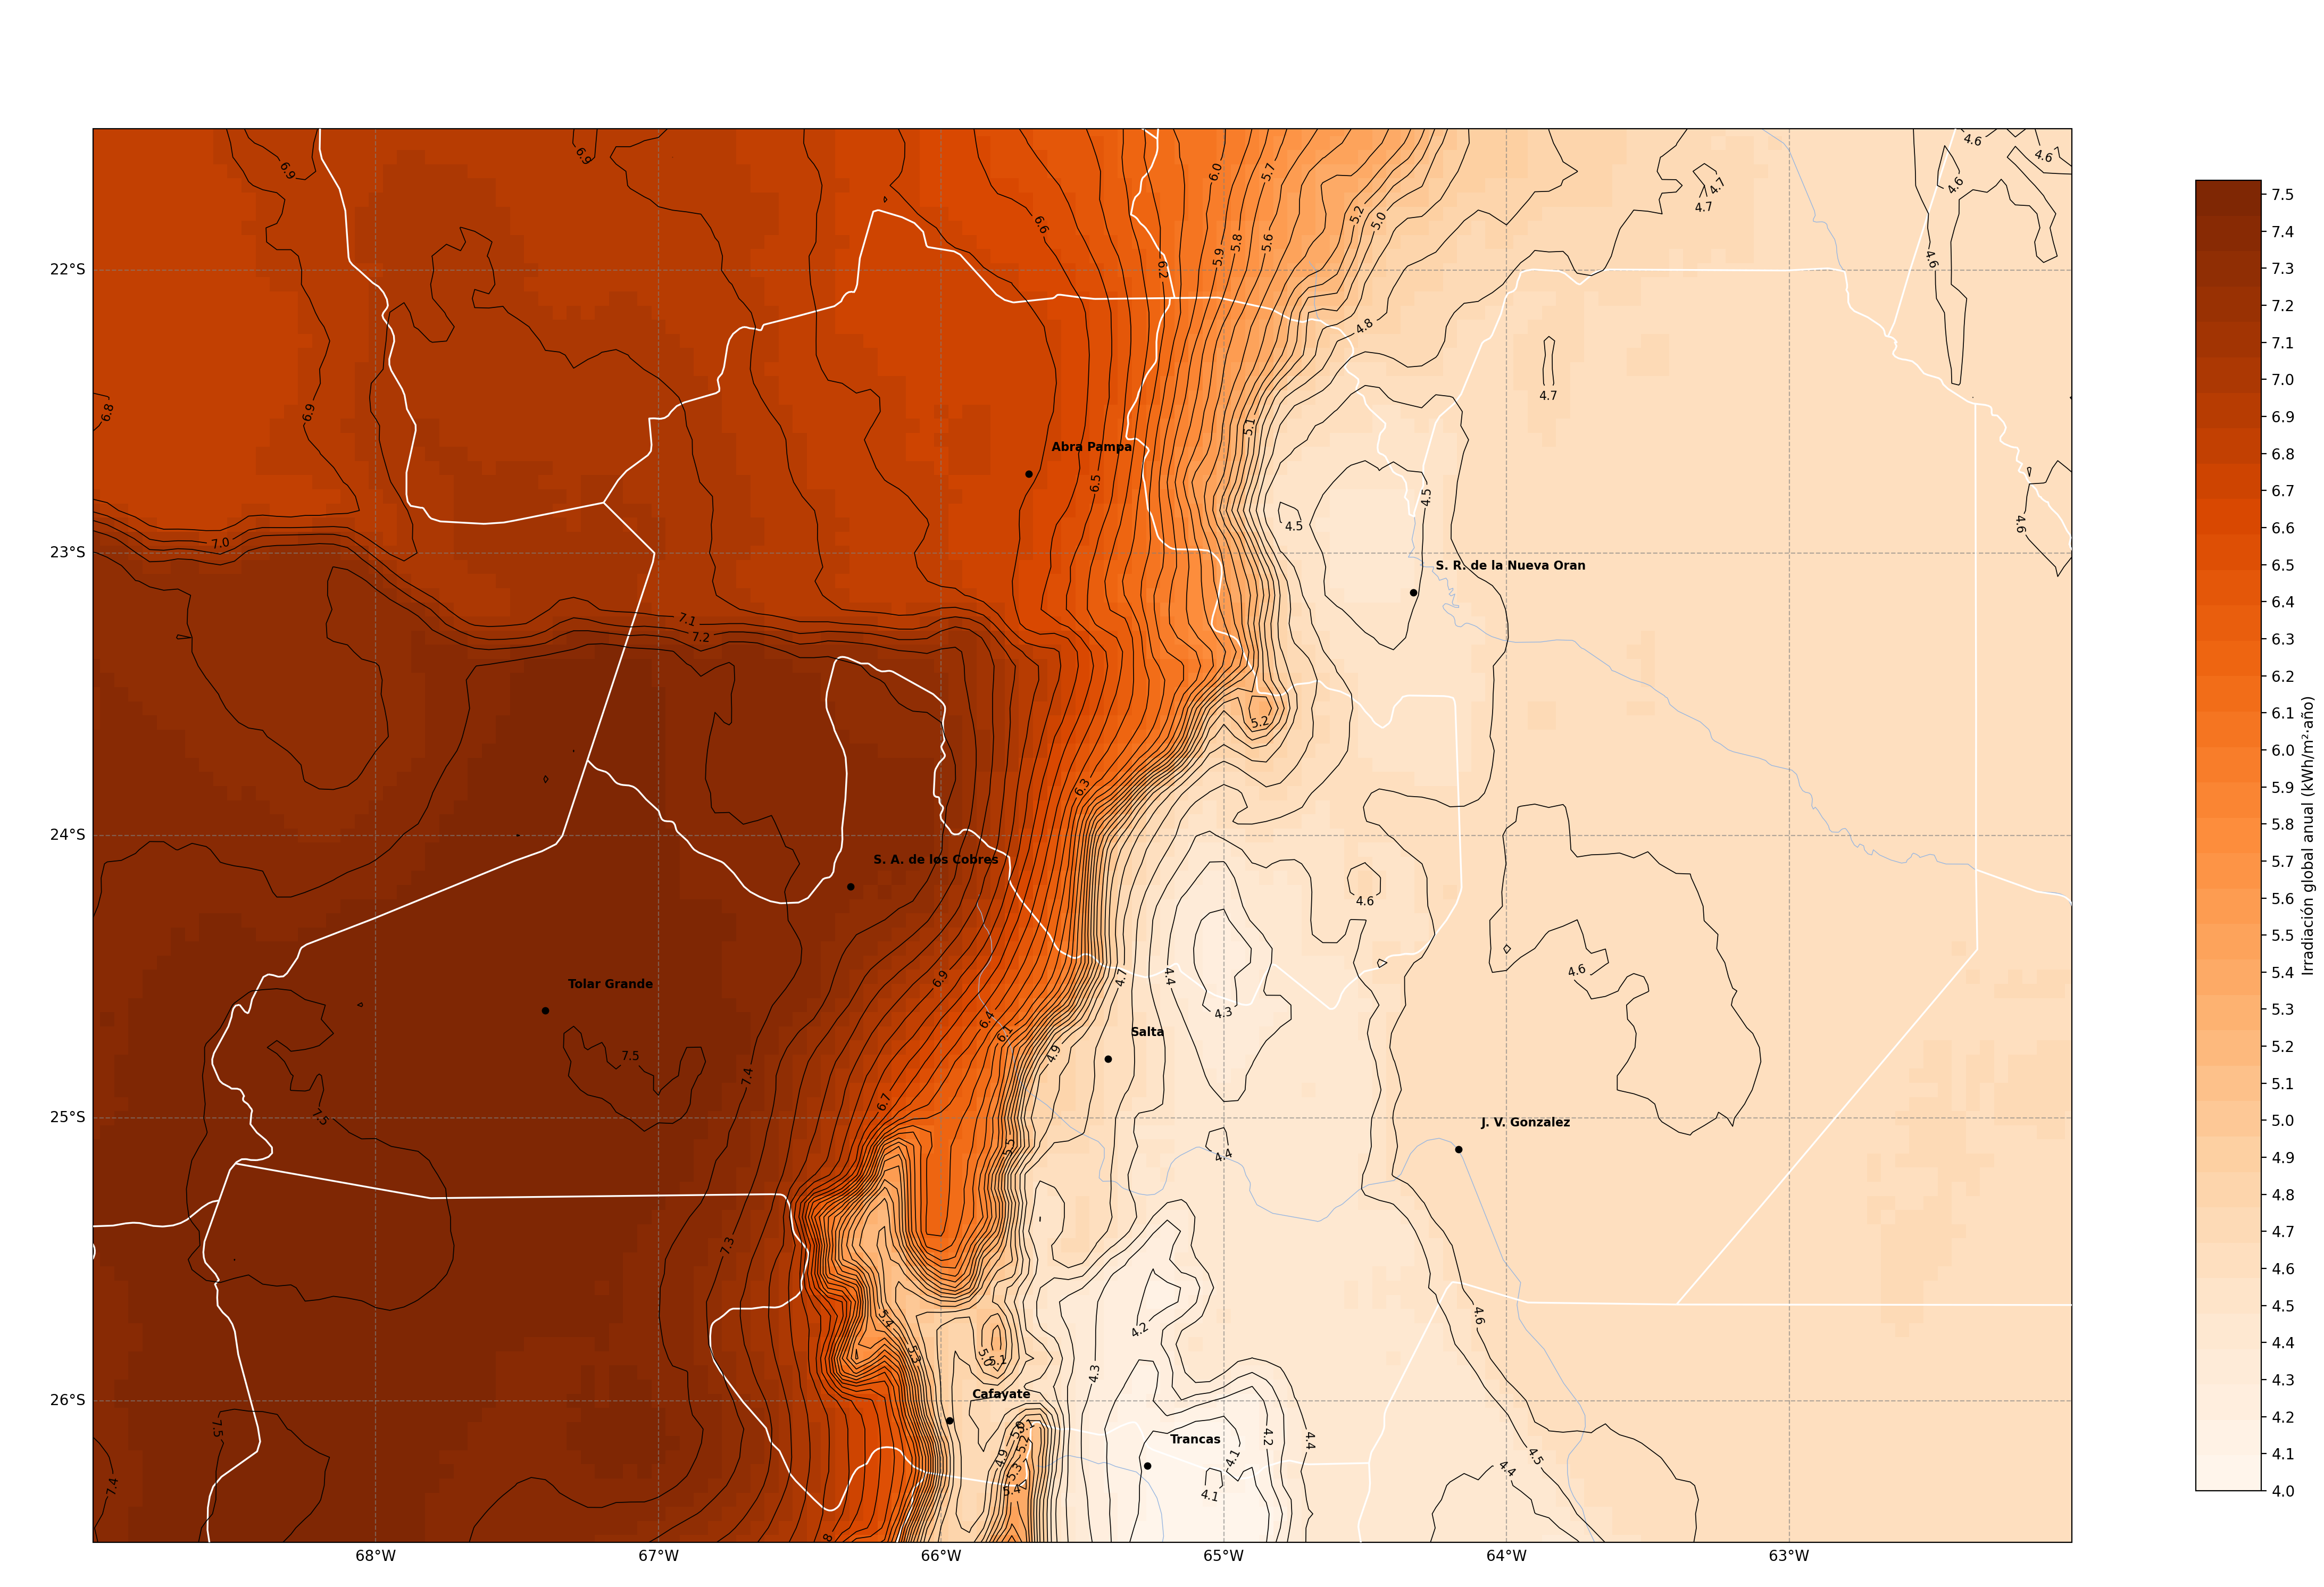
\includegraphics[width=0.99\textwidth]{figuras/Mapas/TMY.png}
    \caption{TMY }
    \label{fig:tmy}
\end{figure} \DIFaddend %Opcional: Comentar si se desea
\DIFdelbegin %DIFDELCMD < \newpage %%%
\addcontentsline{toc}{chapter}{\DIFdel{\textbf{Anexo 3}}} 
%DIFAUXCMD
%DIFDELCMD < \lhead{Anexo 3}
%DIFDELCMD < \rhead{\newtitle}
%DIFDELCMD < \cfoot{\thepage}
%DIFDELCMD < \renewcommand{\headrulewidth}{1pt}
%DIFDELCMD < \renewcommand{\footrulewidth}{1pt}
%DIFDELCMD < \chapter*{Anexo 3}
%DIFDELCMD < \noindent %%%
\DIFdel{En este anexo se incluyen cada una de las publicaciones que se han realizado en el transcurso de esta tesis.
}%DIFDELCMD < 

%DIFDELCMD < \begin{itemize}
\begin{itemize}%DIFAUXCMD
%DIFDELCMD < \item %%%
\item%DIFAUXCMD
\DIFdel{Salazar, G. A., Alonso-Suárez, R., Laguarda Cirigliano, A., \& Ledesma, R. D. (2022). Evaluación del proceso de adaptación al sitio aplicado a la irradiancia solar global medida en la ciudad de Salta, Argentina. Avances En Energías Renovables Y Medio Ambiente - AVERMA, 25, 353–362. 
}%DIFDELCMD < \item %%%
\item%DIFAUXCMD
\DIFdel{Ledesma, R. D., Salazar, G. A., \& de Castro Vilela, O. (2022). Aplicación móvil como herramienta para la evaluación de modelos de irradiancia solar. En Acta de la XLIV Reunión de Trabajo de la Asociación Argentina de Energías Renovables y Ambiente (Vol. 9, pp. 186–195). ISBN 978-987-29873-1-2.
}%DIFDELCMD < 

%DIFDELCMD < \item %%%
\item%DIFAUXCMD
\DIFdel{Ledesma, R. D., Salazar, G. A., \& de Castro Vilela, O. (2022). ARGP-V2: Un modelo práctico para la estimación de irradiancia global horizontal en condiciones de cielo claro para sitios de altura. Avances en Energías Renovables y Medio Ambiente, 26, 283–289. ISSN 2796-8111. ASADES 2022.
}%DIFDELCMD < 

%DIFDELCMD < \item %%%
\item%DIFAUXCMD
\DIFdel{Ledesma, R., Alonso-Suárez, R., Monetta, A., Laguarda, A., Vilela, O., \& Salazar, G. (2024). Evaluación en Uruguay del producto DSR GOES-16 de irradiancia solar global horizontal. Avances En Energías Renovables Y Medio Ambiente - AVERMA, 27, 474–483.
}%DIFDELCMD < 

%DIFDELCMD < \item %%%
\item%DIFAUXCMD
\DIFdel{Ledesma, R., Salazar, G., \& Vilela, O. (2024). Avances en la estimación de irradiancia solar en las provincias de Salta y jujuy mediante imágenes satelitales GOES-16. Avances En Energías Renovables Y Medio Ambiente - AVERMA, 27, 413–427.
}%DIFDELCMD < 

%DIFDELCMD < \item %%%
\item%DIFAUXCMD
\DIFdel{Salazar, G., Ledesma, R. D., López Ruiz, C. ., \& de Castro Vilela, O. (2025). Análisis de desempeño de diferentes técnicas de aprendizaje automático en una adaptación al sitio de irradiancia solar global para Salta (Argentina). Avances En Energías Renovables Y Medio Ambiente - AVERMA, 28, 308–320.
}%DIFDELCMD < 

%DIFDELCMD < \item %%%
\item%DIFAUXCMD
\DIFdel{López Ruiz, C. B., Salazar, G. A., Ledesma, R., \& Bezerra Galdino, J. J. (2025, marzo). Análisis de radiación solar difusa medida usando banda sombreadora: Caso de estudio en la ciudad de Salta. En Acta de la XLVI Reunión de Trabajo de la Asociación Argentina de Energías Renovables y Ambiente (Vol. 11, pp. 236–248). ISBN 978-987-29873-1-2.
}%DIFDELCMD < 

%DIFDELCMD < \item %%%
\item%DIFAUXCMD
\DIFdel{Salazar, G., Ledesma, R., López Ruiz, C., \& Castro Vilela, O. (2024). Development of a solar irradiance cloud index model for Northwest Argentina using GOES-16 imagery: Comparison against reanalysis and satellite databases. En International Academy of Astronautics (Ed.), Proceedings of the International Academy of Astronautics Latin American Conference on Small Satellite Technologies and Applications (1.ª ed., pp. 191-197). International Academy of Astronautics. ISBN 978-2-917761-85-4.
}%DIFDELCMD < 

%DIFDELCMD < \item %%%
\item%DIFAUXCMD
\DIFdel{Ledesma, R., Alonso-Suárez, R., Salazar, G., Nollas, F., \& Vilela, O. (2025). Evaluation of satellite and reanalysis models for solar irradiance estimation in Northwest Argentina. IEEE Latin America Transactions, 23(8), 706–717. https://doi.org/10.1109/TLA.2025.11072498.
}%DIFDELCMD < 

%DIFDELCMD < \item %%%
\item%DIFAUXCMD
\DIFdel{Silvero, C. I., Forciniti, J. D., Medina, F. D., Vega Caro, M. A., Ledesma, R. D., Zossi, B. S., Mansilla, G. A., and Elias, A. G. (October 10, 2025). "Comparative Study of Solar Radiation Measurements in Tucuman, Argentina, With Reanalyses and Satellite-Based Datasets." ASME. J. Sol. Energy Eng. December 2025; 147(6): 061012.
}%DIFDELCMD < 

%DIFDELCMD < \item %%%
\item%DIFAUXCMD
\DIFdel{Ledesma, R., Salazar, G.. (2025). Machine learning for site adaptation of satellite-derived solar irradiance in Northwestern Argentina. Journal of Computer Science and Technology, 25(2), e10. https://doi.org/10.24215/16666038.25.e10
}%DIFDELCMD < \item %%%
\item%DIFAUXCMD
\DIFdel{Cinco Reynaga, P., \& Ledesma, R. D. (en prensa). Evaluación de algoritmos de aprendizaje automático para la clasificación de días de cielo claro. En Actas de la XLVI Reunión de Trabajo de la Asociación Argentina de Energías Renovables y Ambiente (AVERMA) (Vol. 11, pp. 236–248). ISBN 978-987-29873-1-2.
}
\end{itemize}%DIFAUXCMD
%DIFDELCMD < \end{itemize}
%DIFDELCMD < 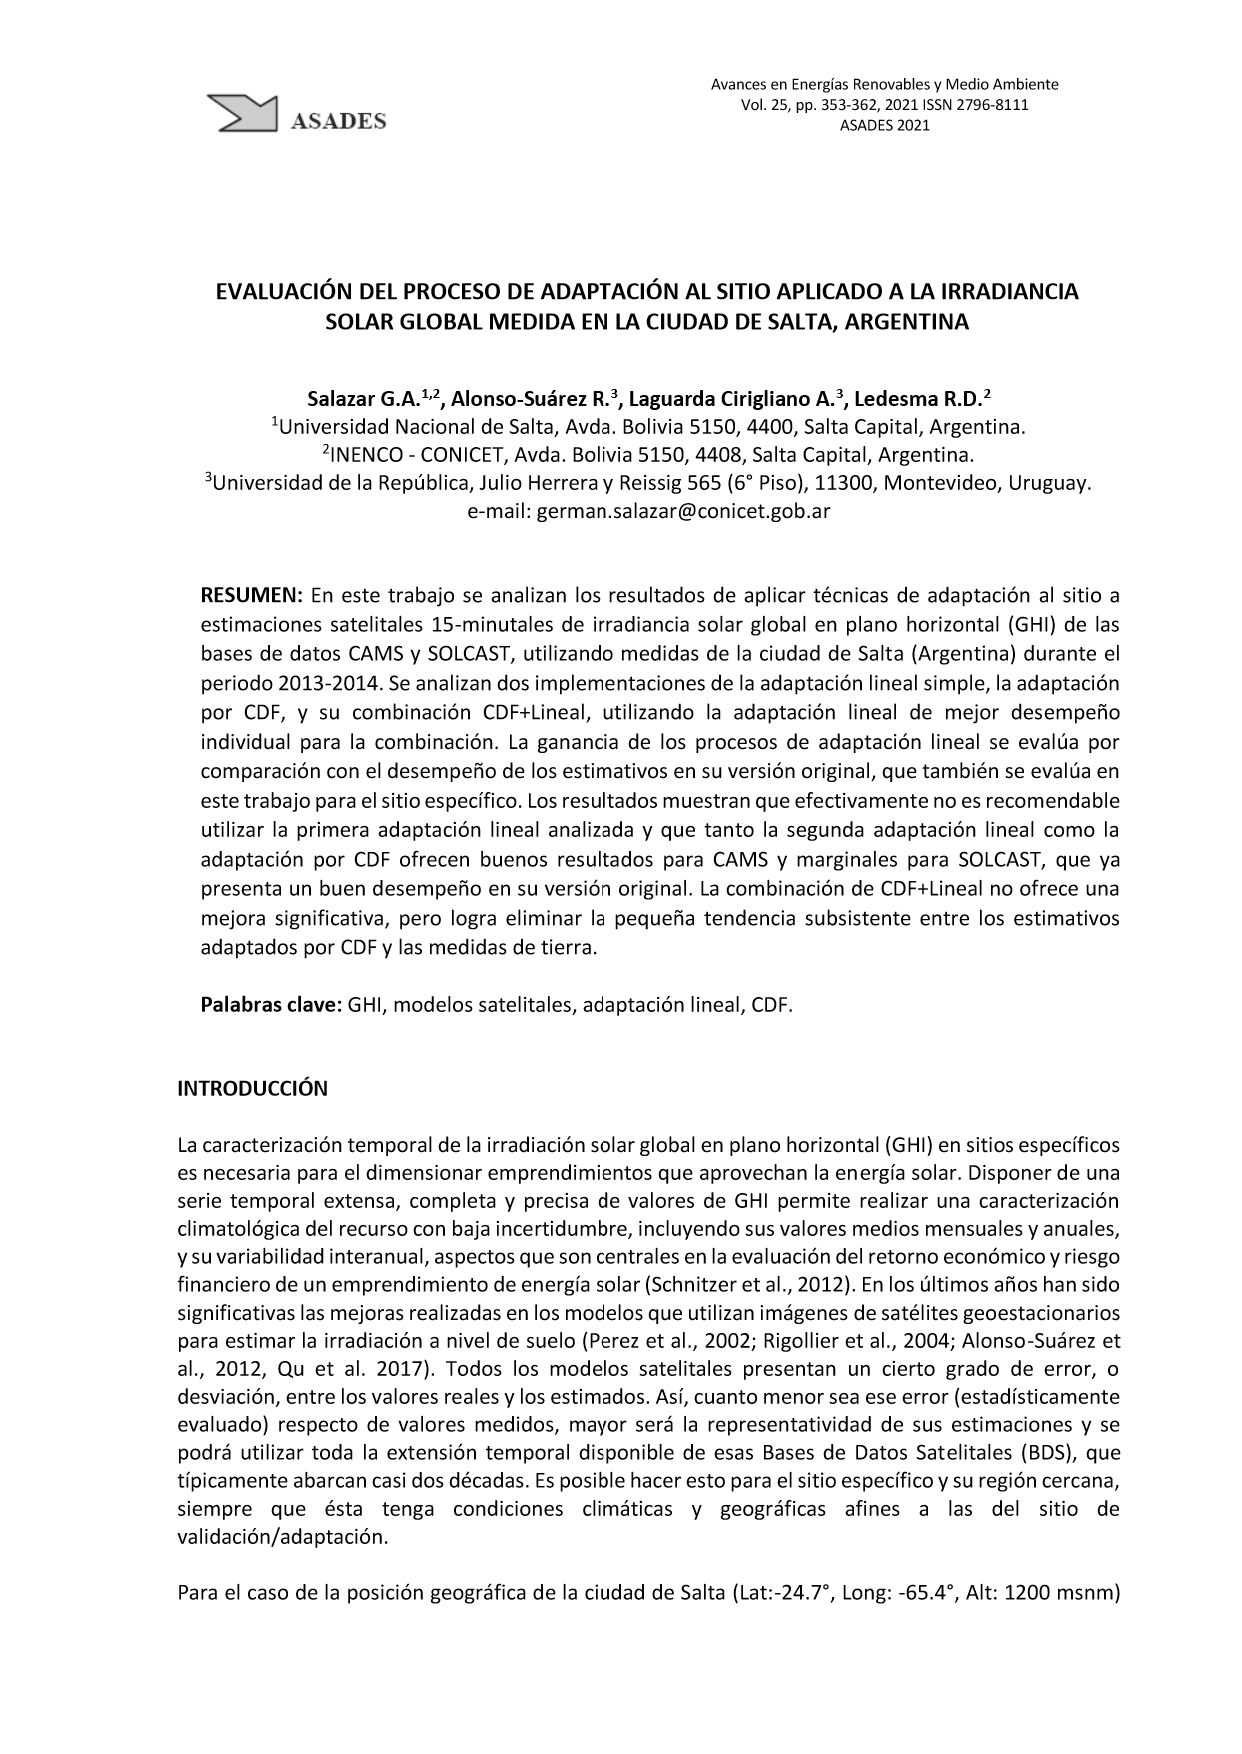
\includepdf[pages=-]{anexo_3/01_site_adaptation2}
%DIFDELCMD < 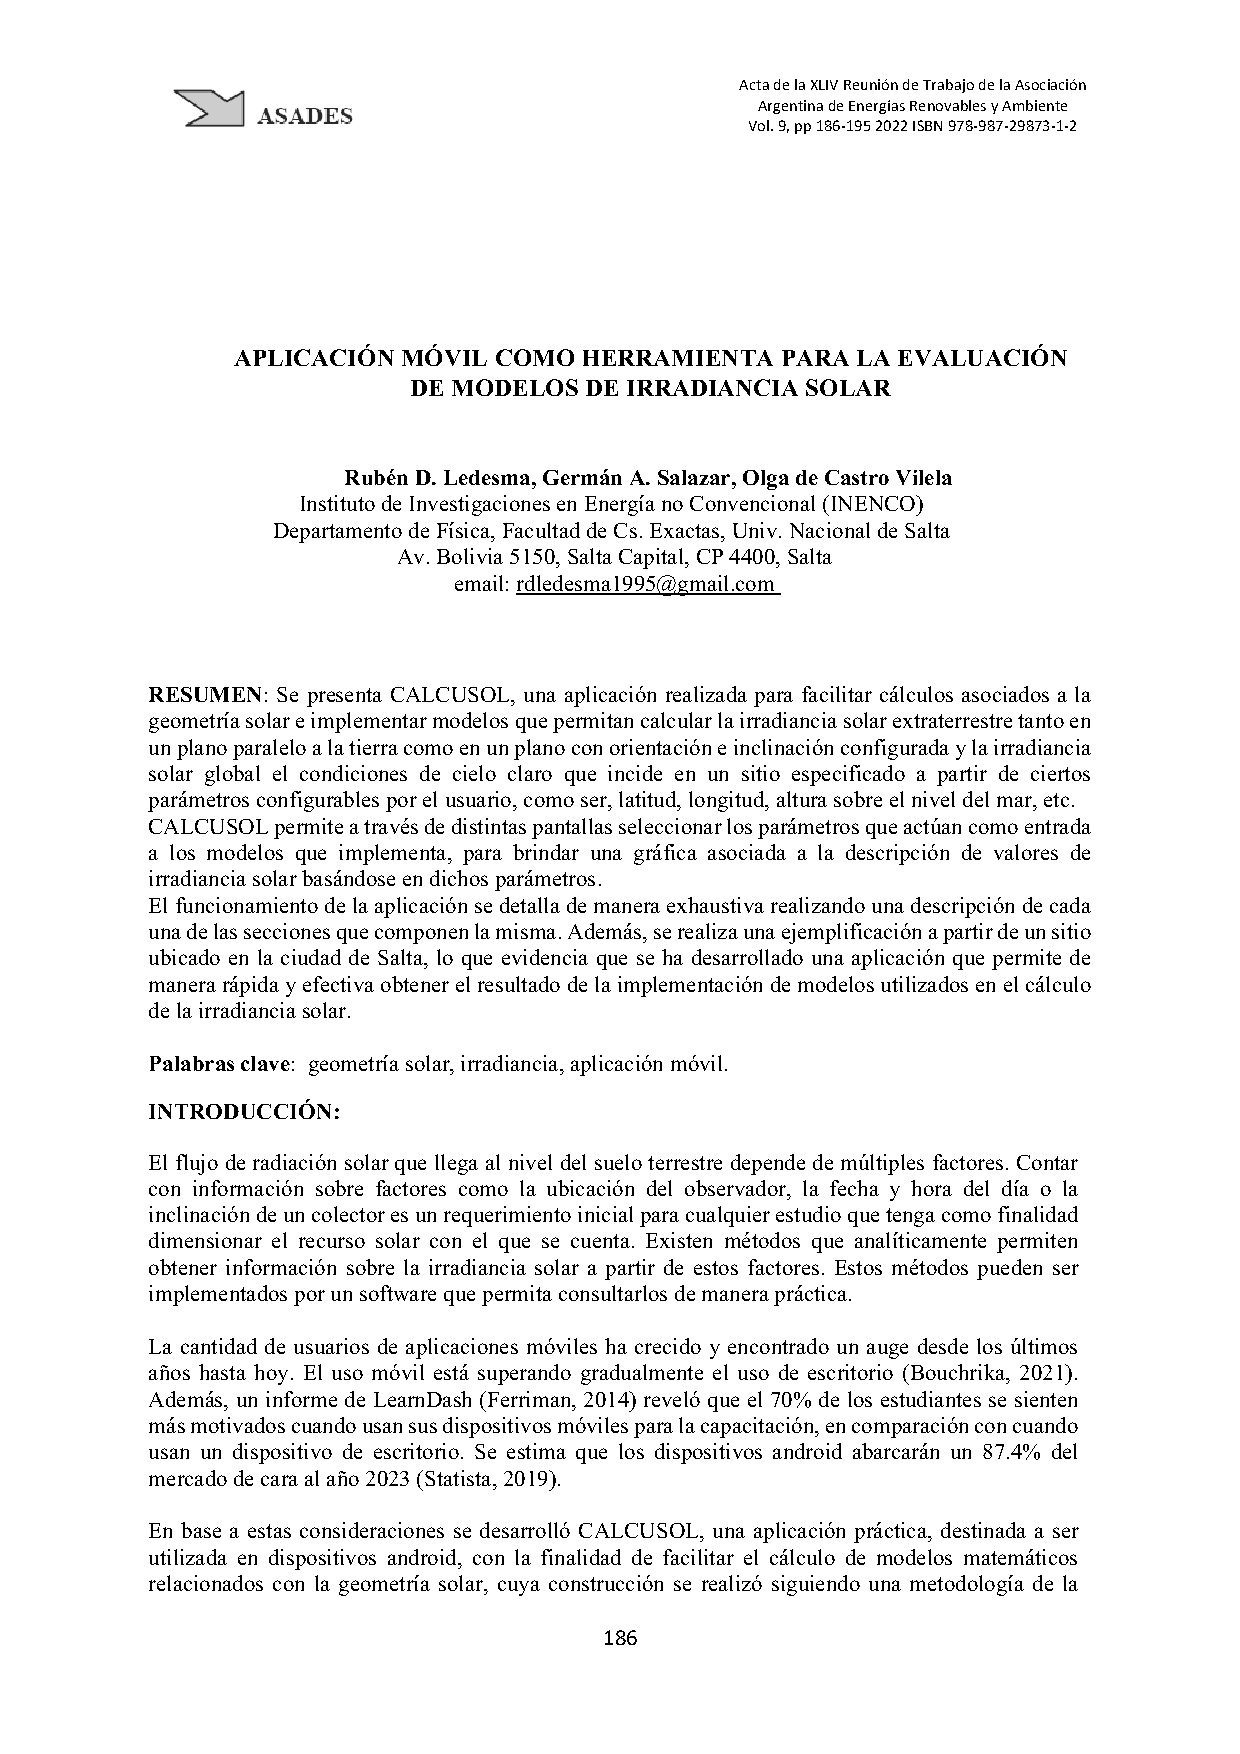
\includepdf[pages=-]{anexo_3/02_Calcusol}
%DIFDELCMD < 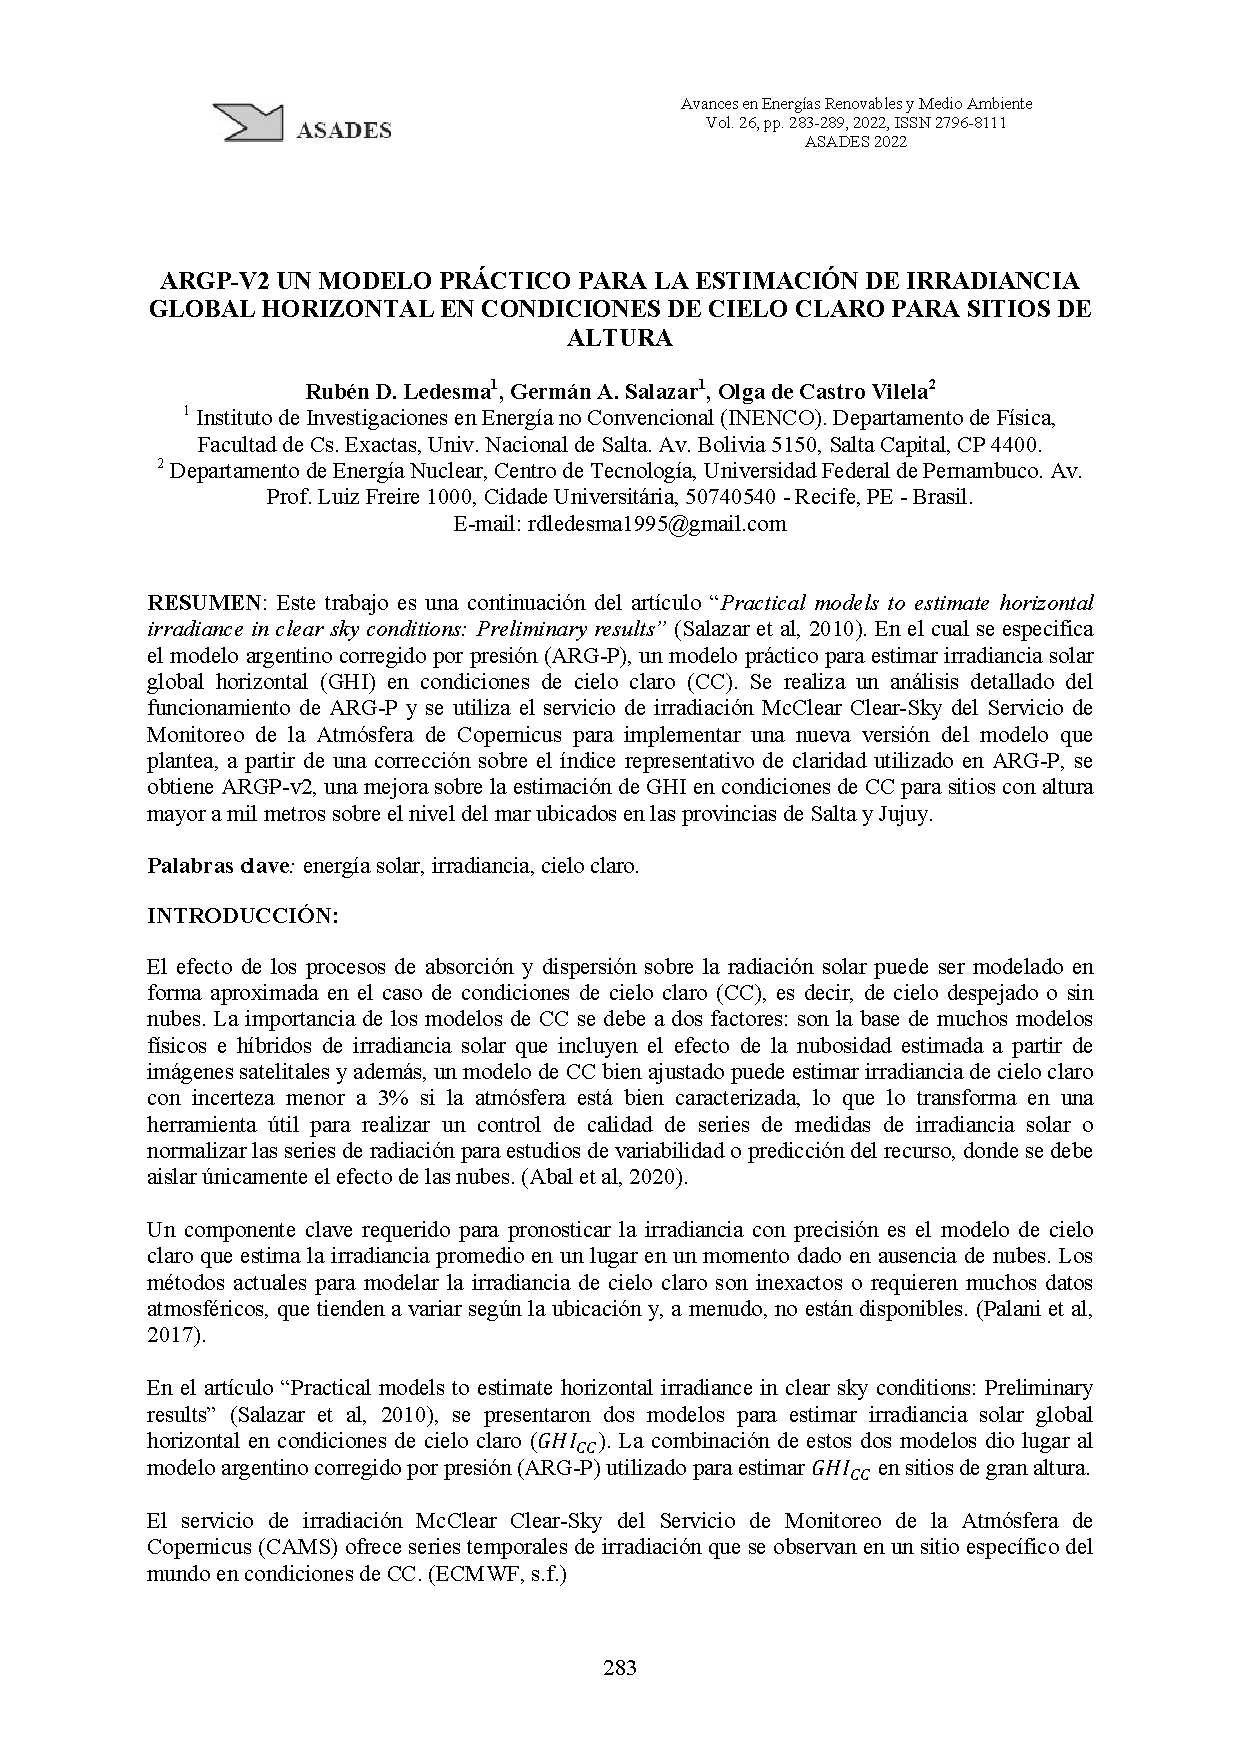
\includepdf[pages=-]{anexo_3/03_argp}
%DIFDELCMD < 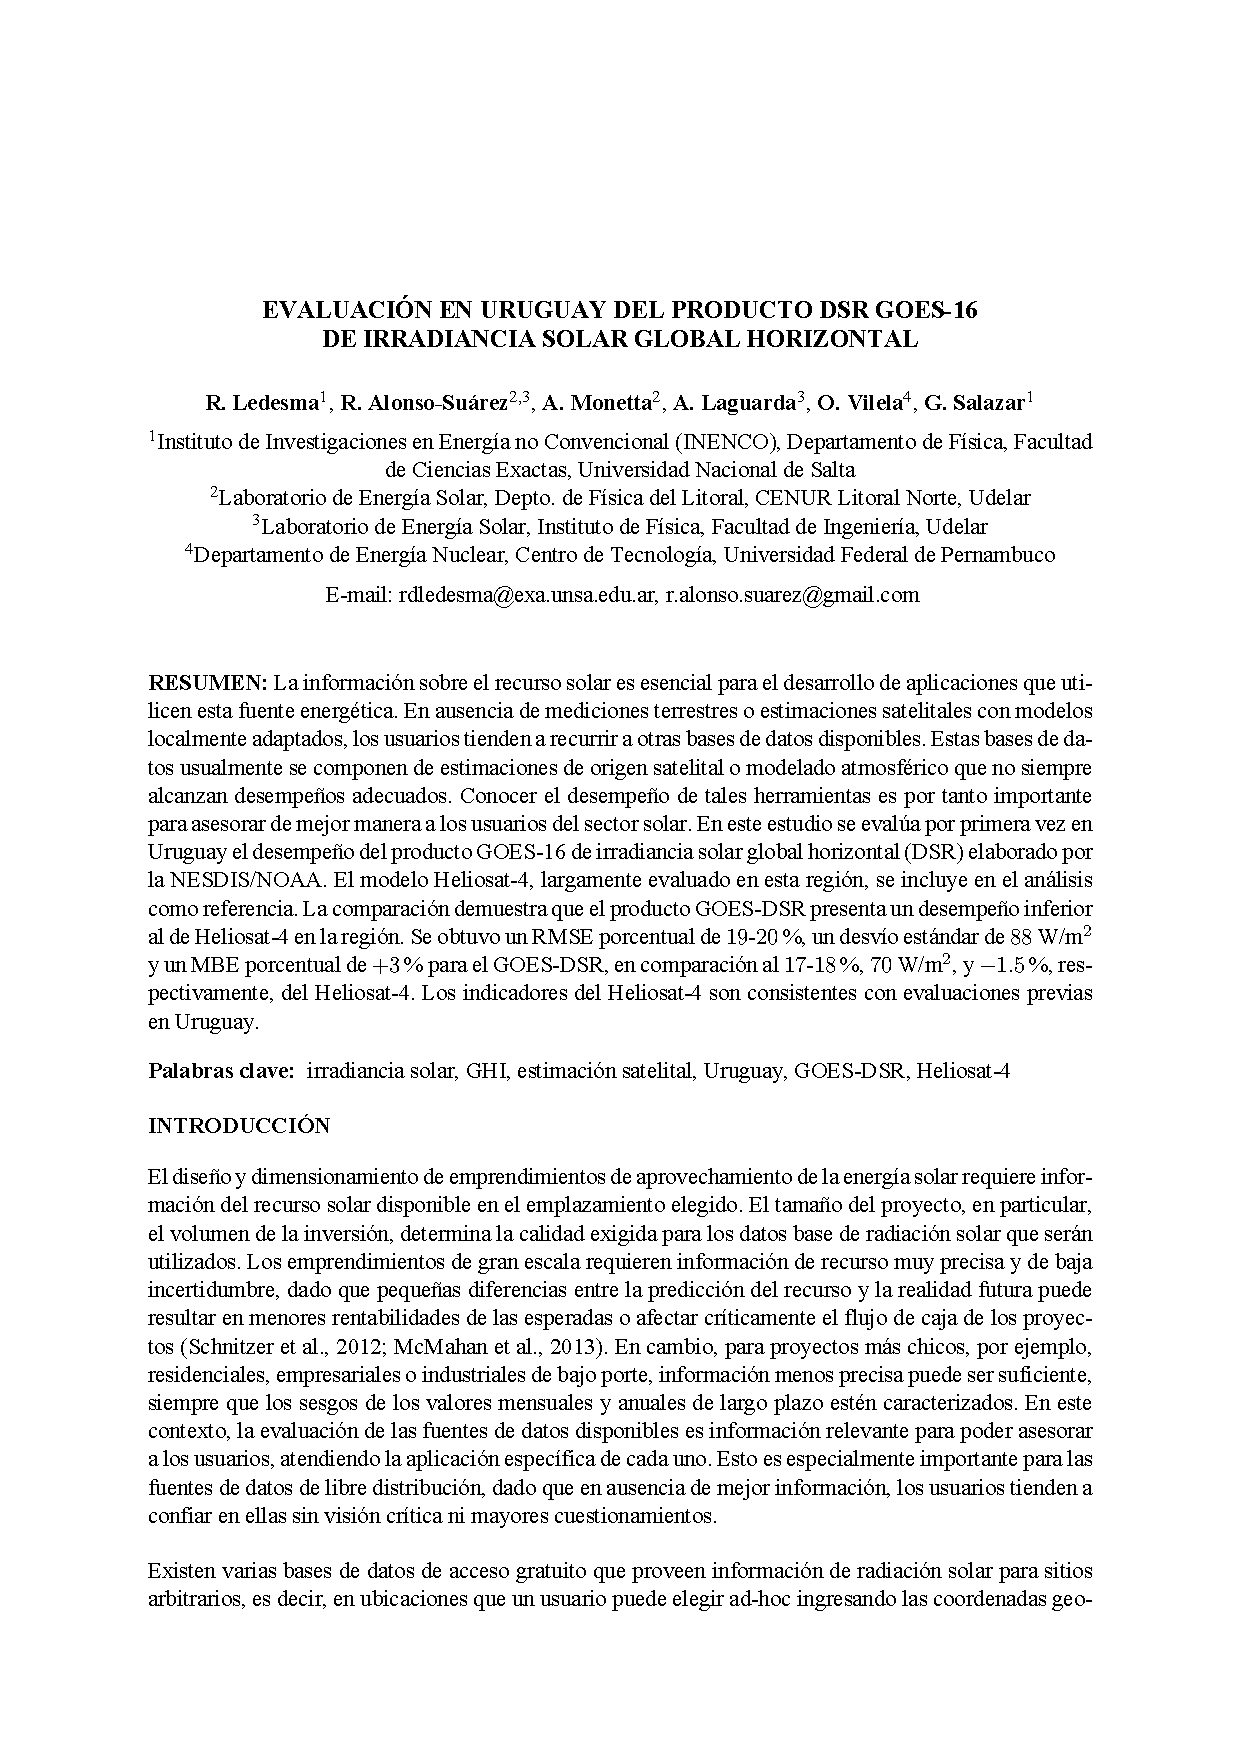
\includepdf[pages=-]{anexo_3/04_DSR}
%DIFDELCMD < 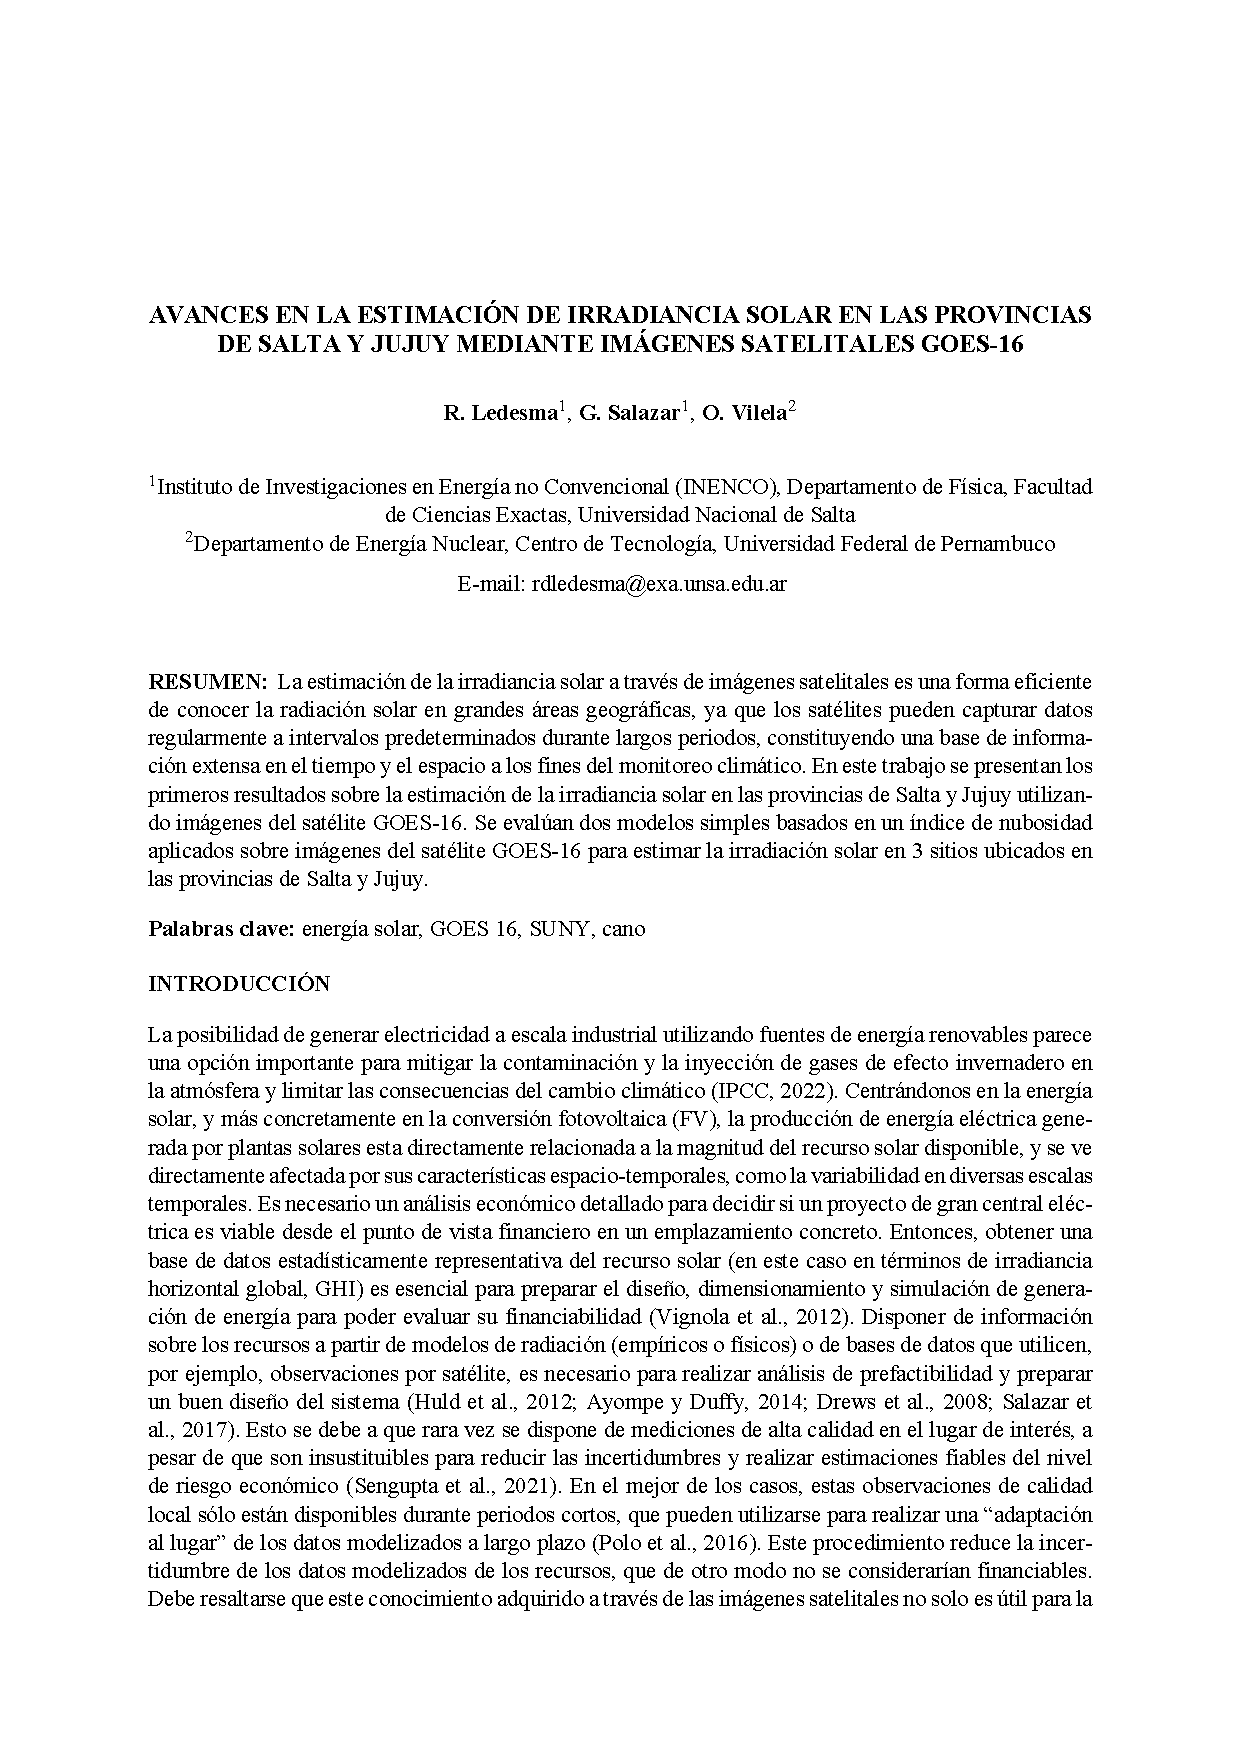
\includepdf[pages=-]{anexo_3/05_GCIM}
%DIFDELCMD < 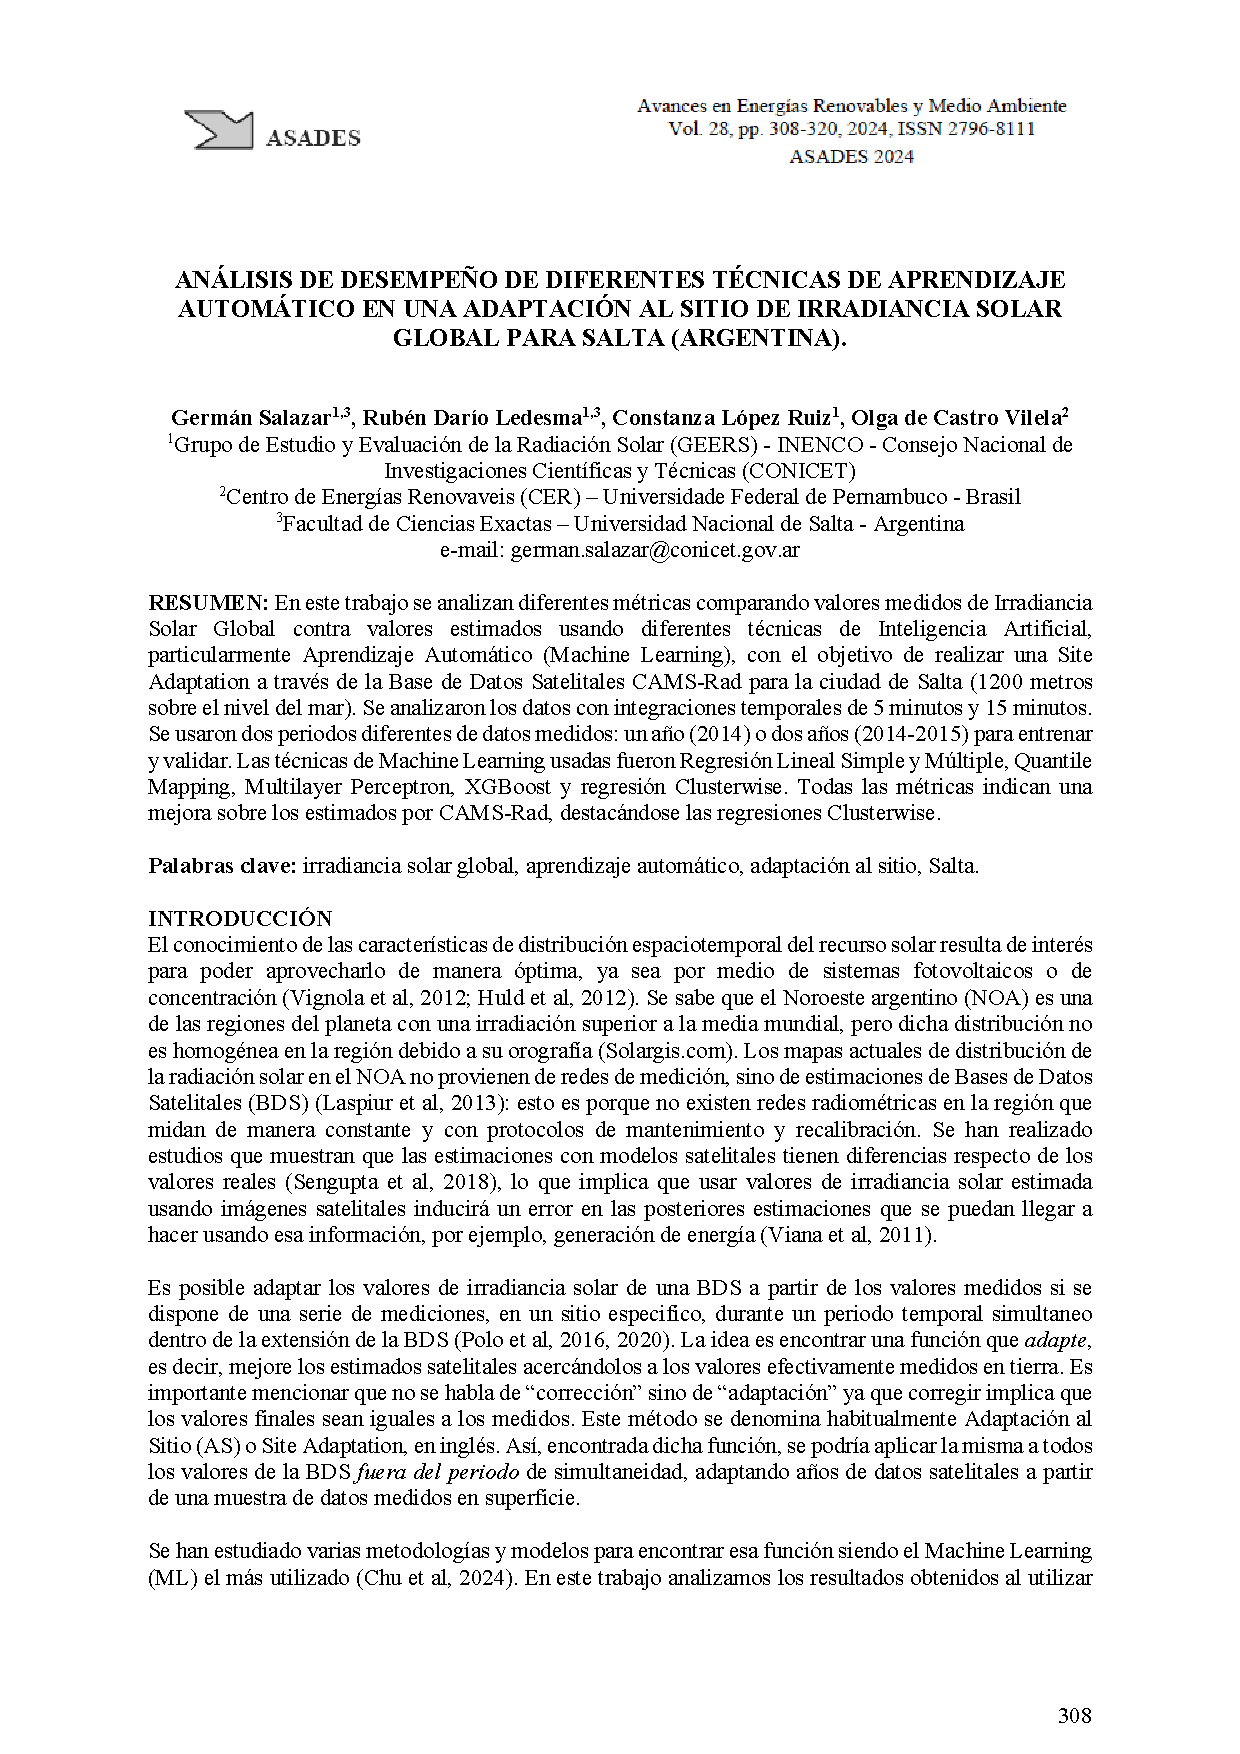
\includepdf[pages=-]{anexo_3/06_DESEMPEÑO}
%DIFDELCMD < 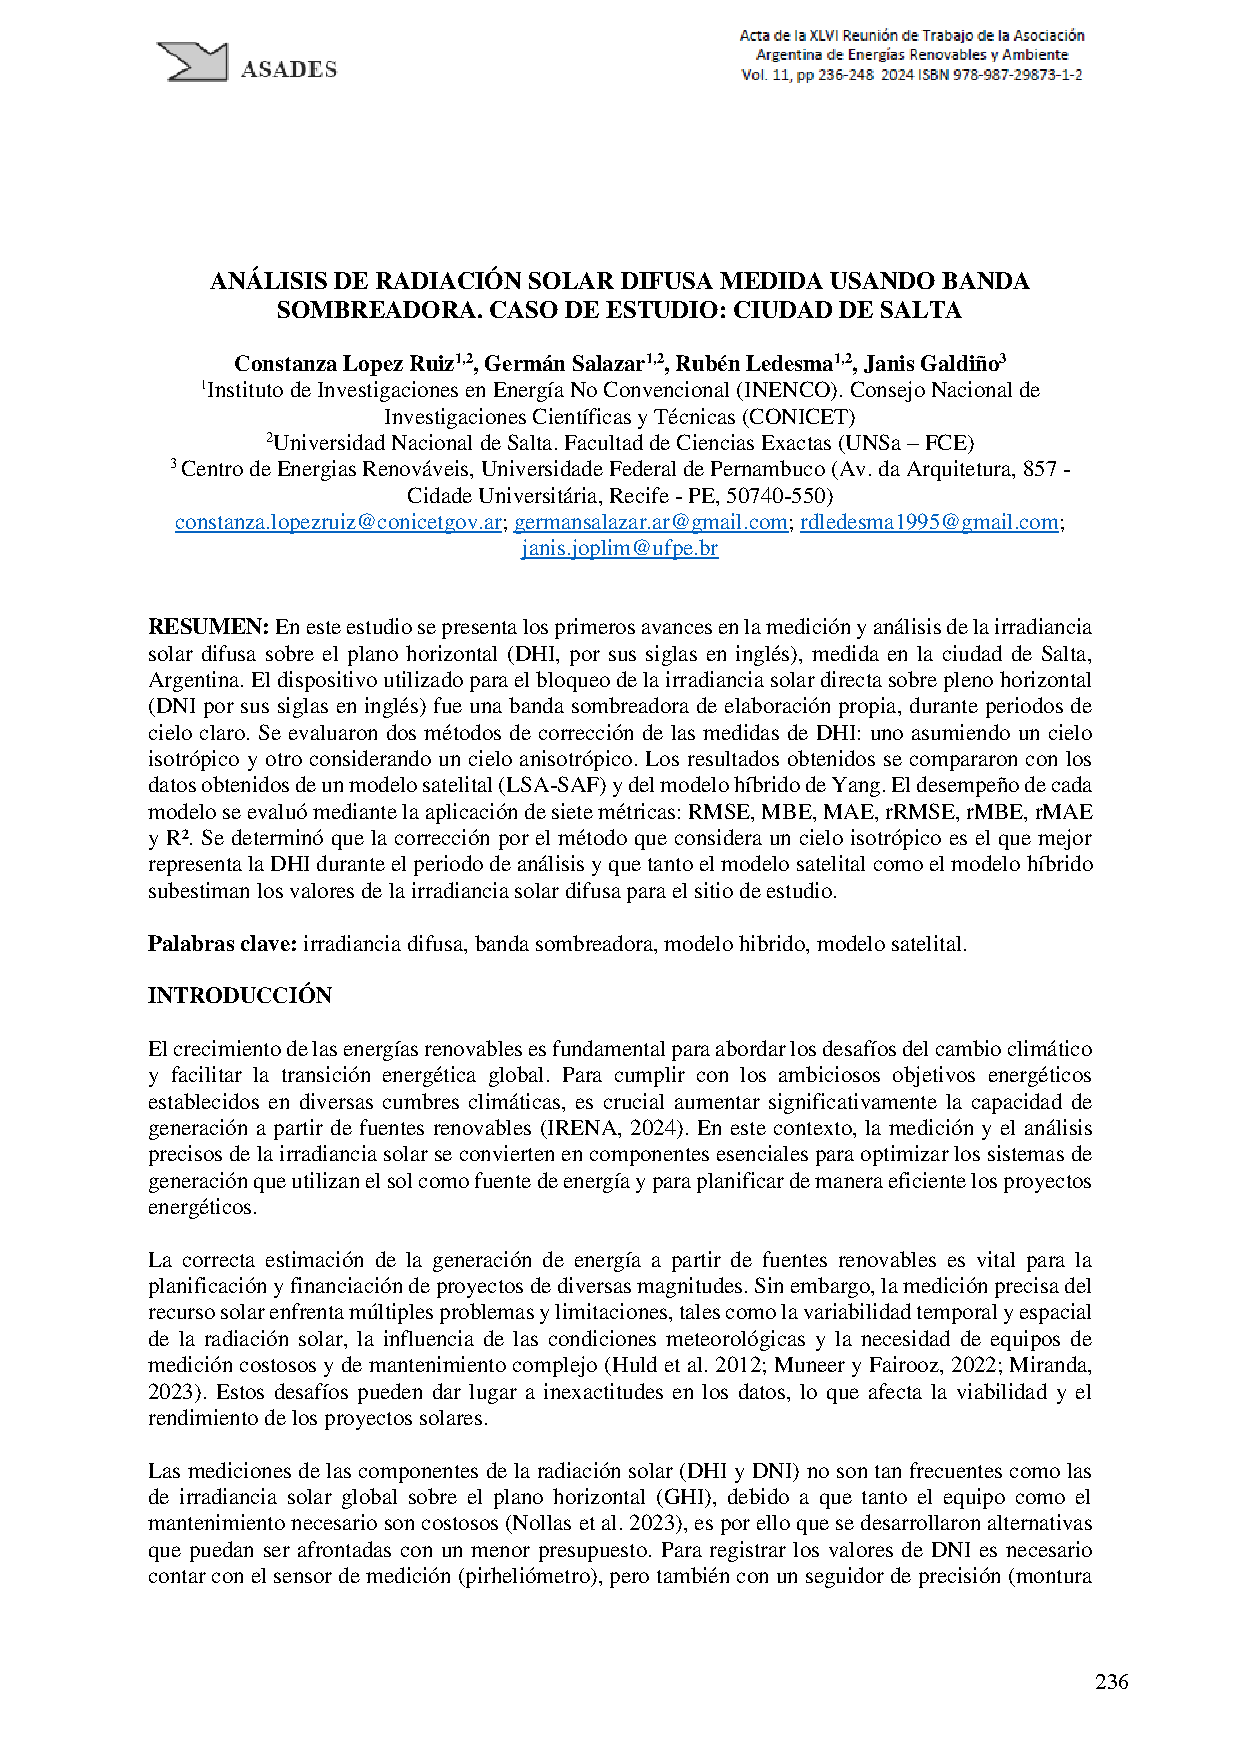
\includepdf[pages=-]{anexo_3/07_DIFUSA}
%DIFDELCMD < 
\includepdf[pages=-]{anexo_3/08_small}
%DIFDELCMD < 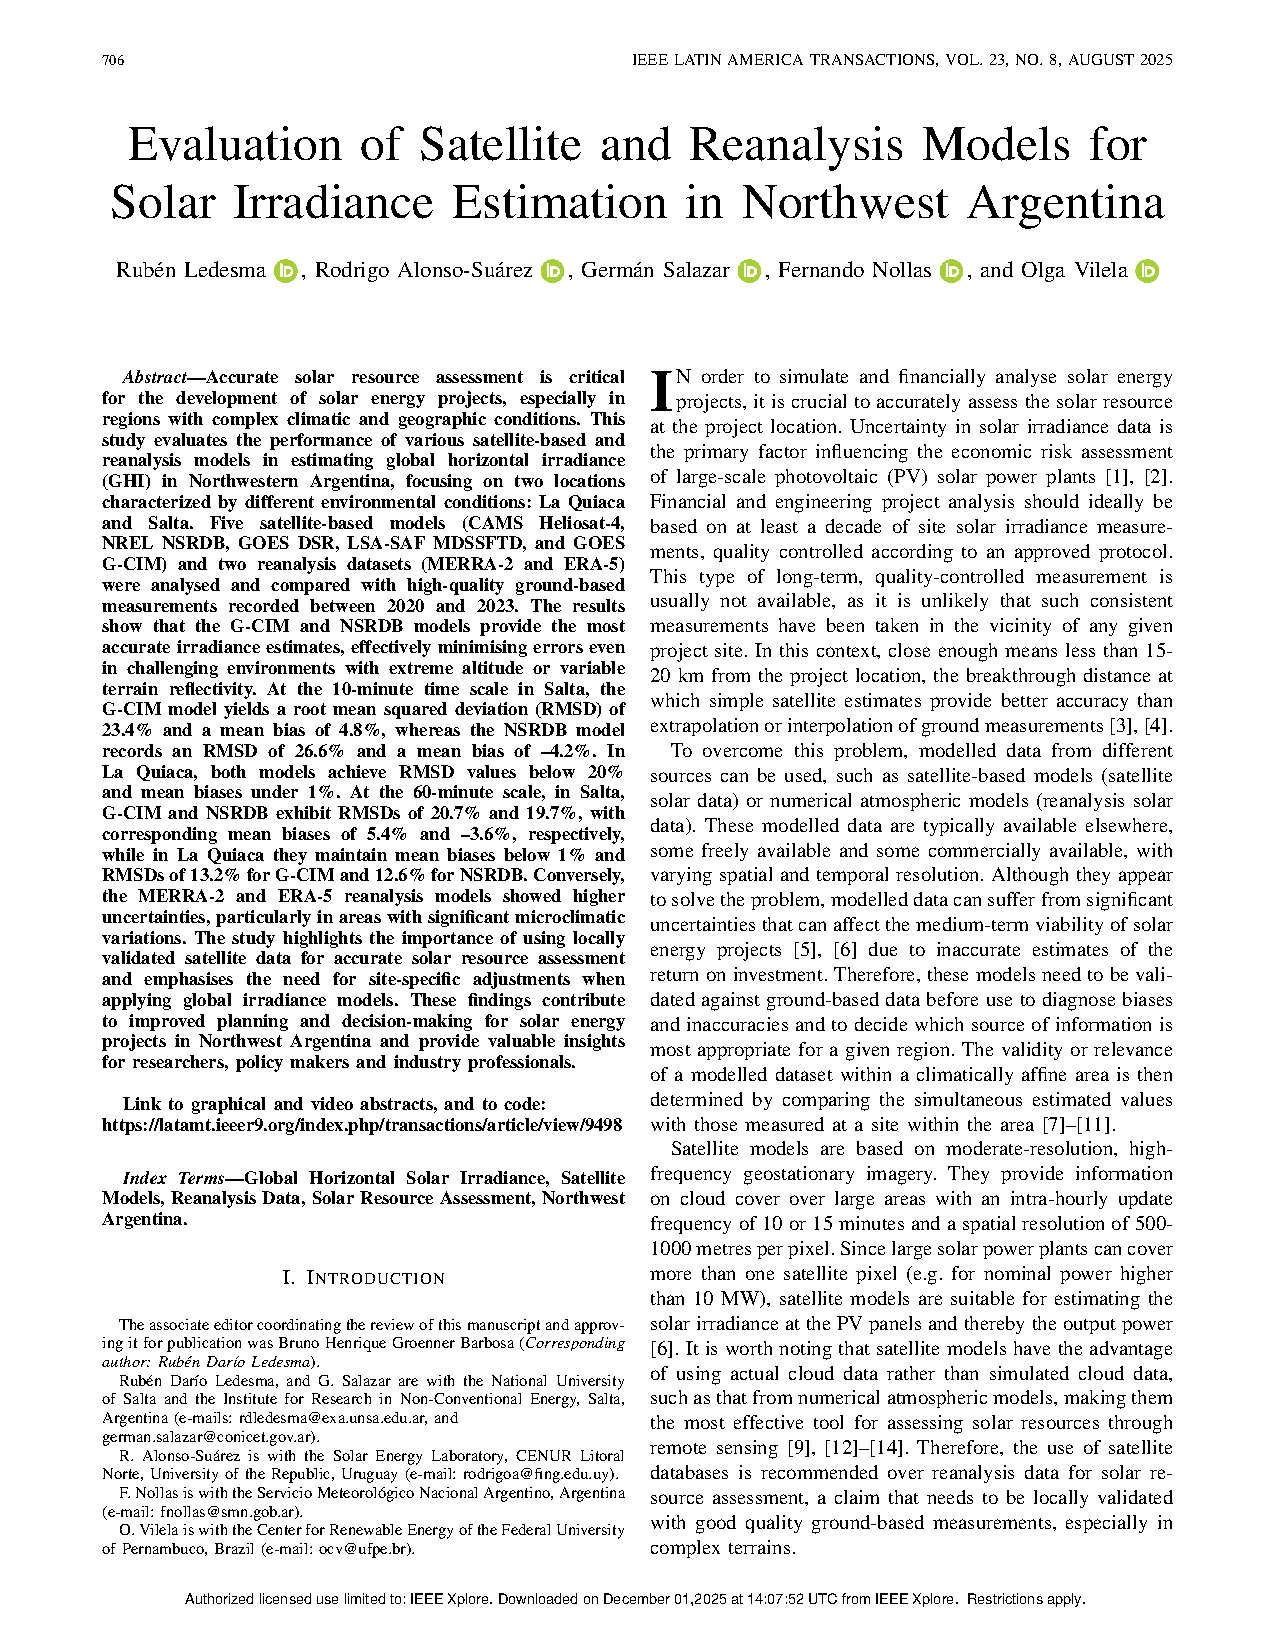
\includepdf[pages=-]{anexo_3/09_IEEE}
%DIFDELCMD < 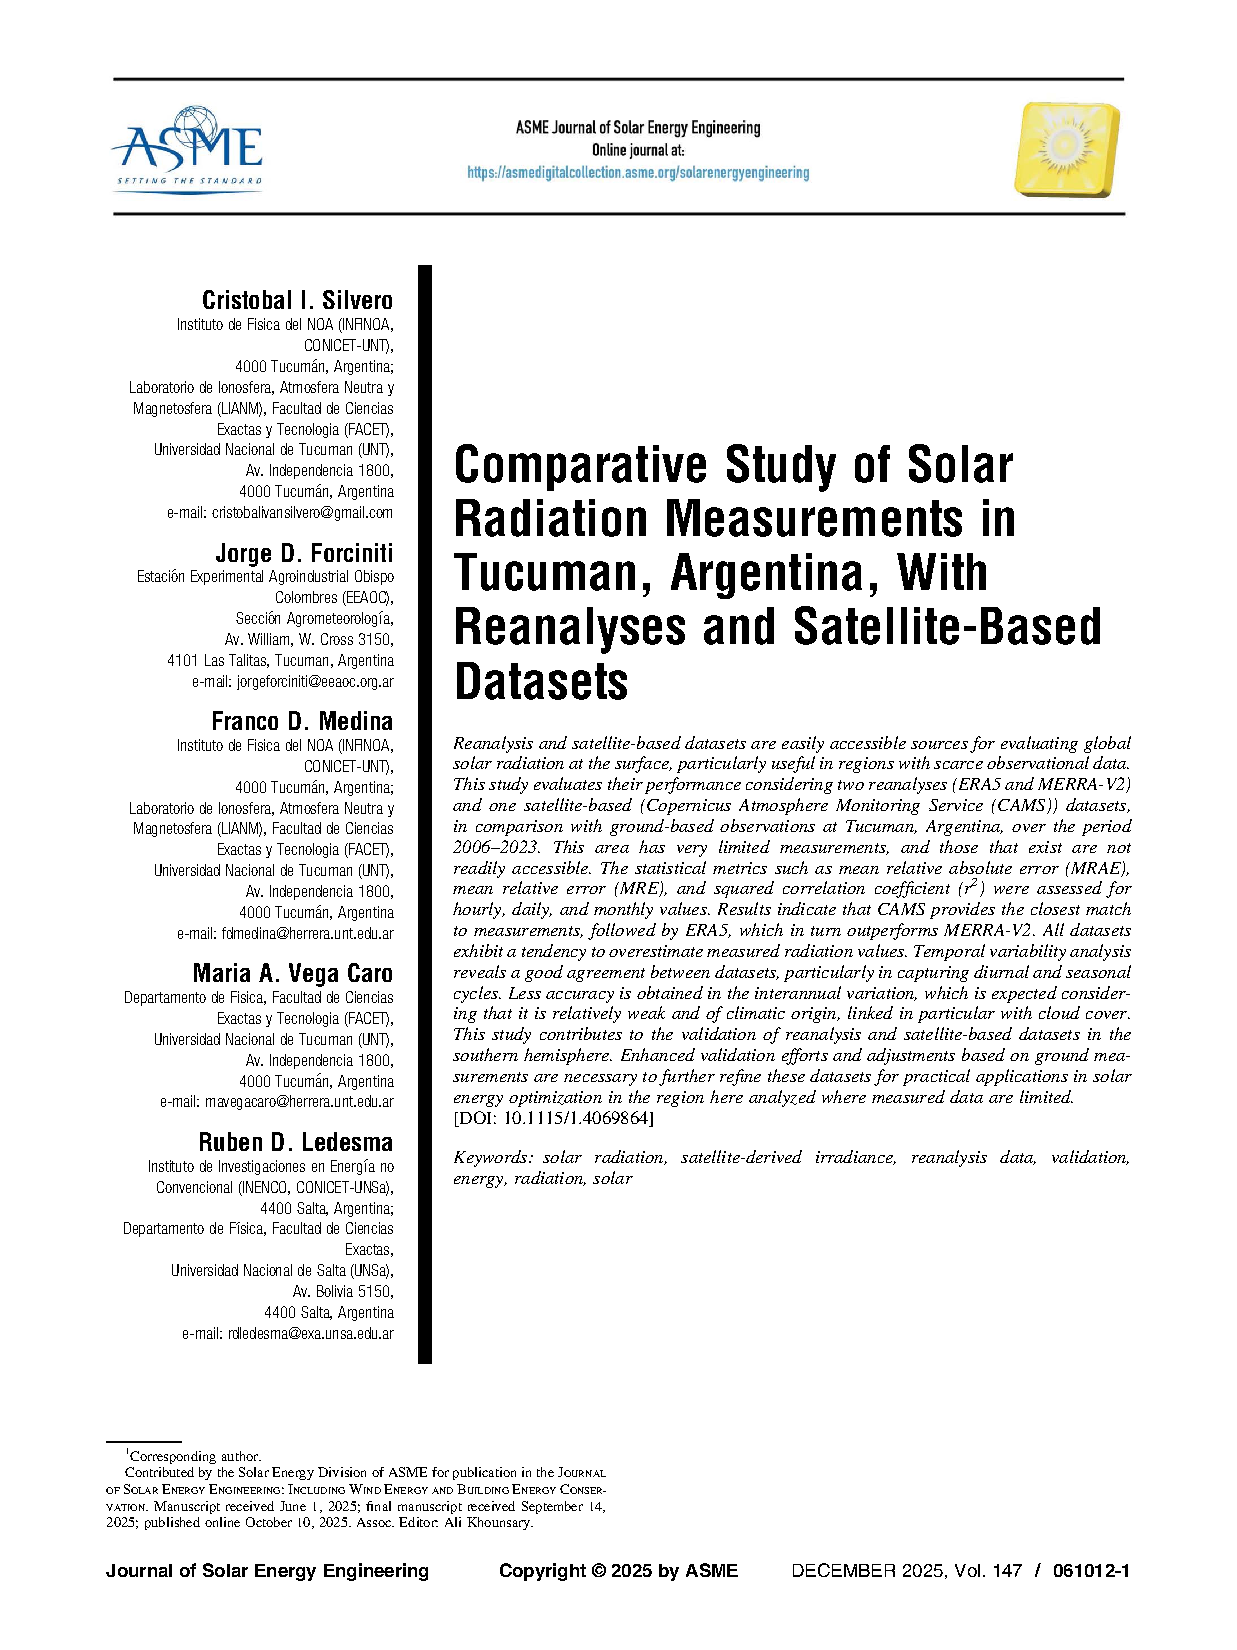
\includepdf[pages=-]{anexo_3/10_SOL}
%DIFDELCMD < 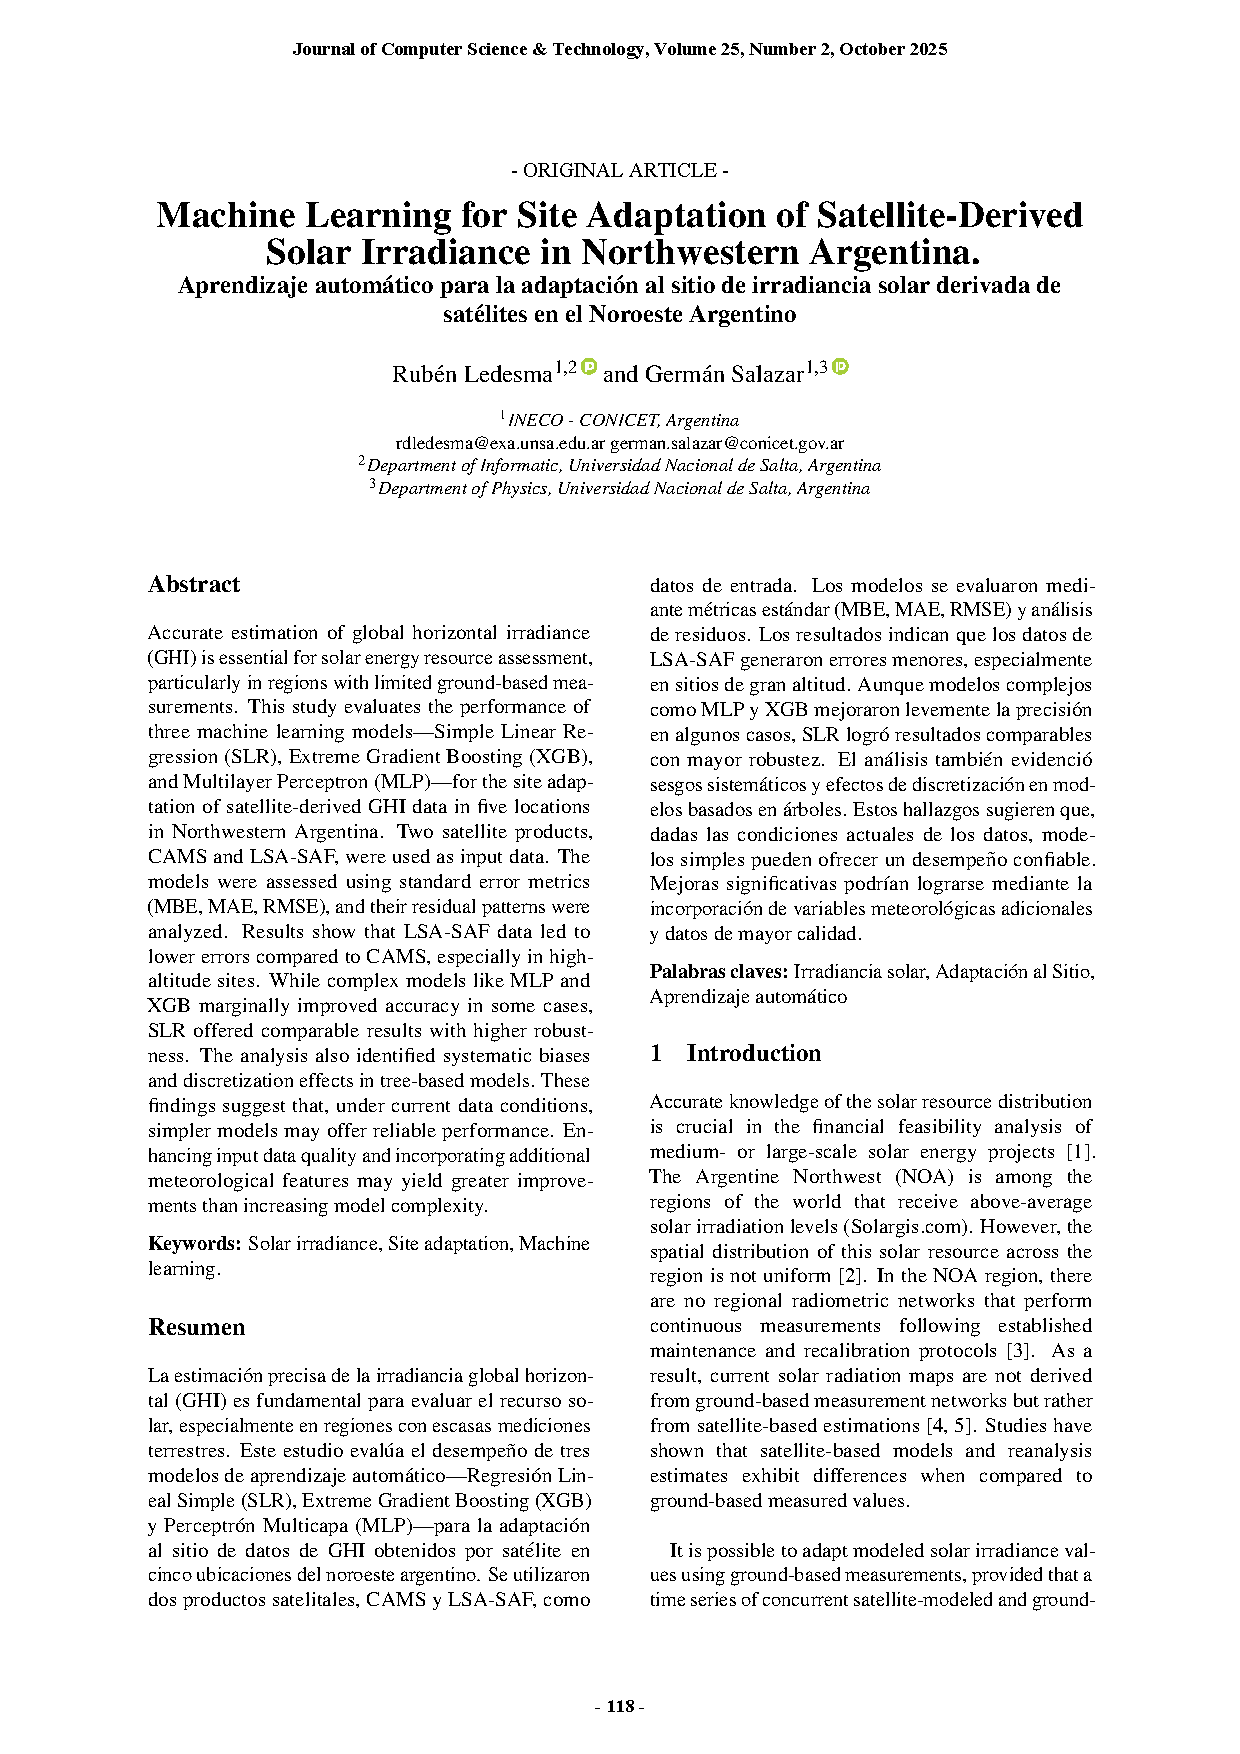
\includepdf[pages=-]{anexo_3/11_ML_JCTS}
%DIFDELCMD < 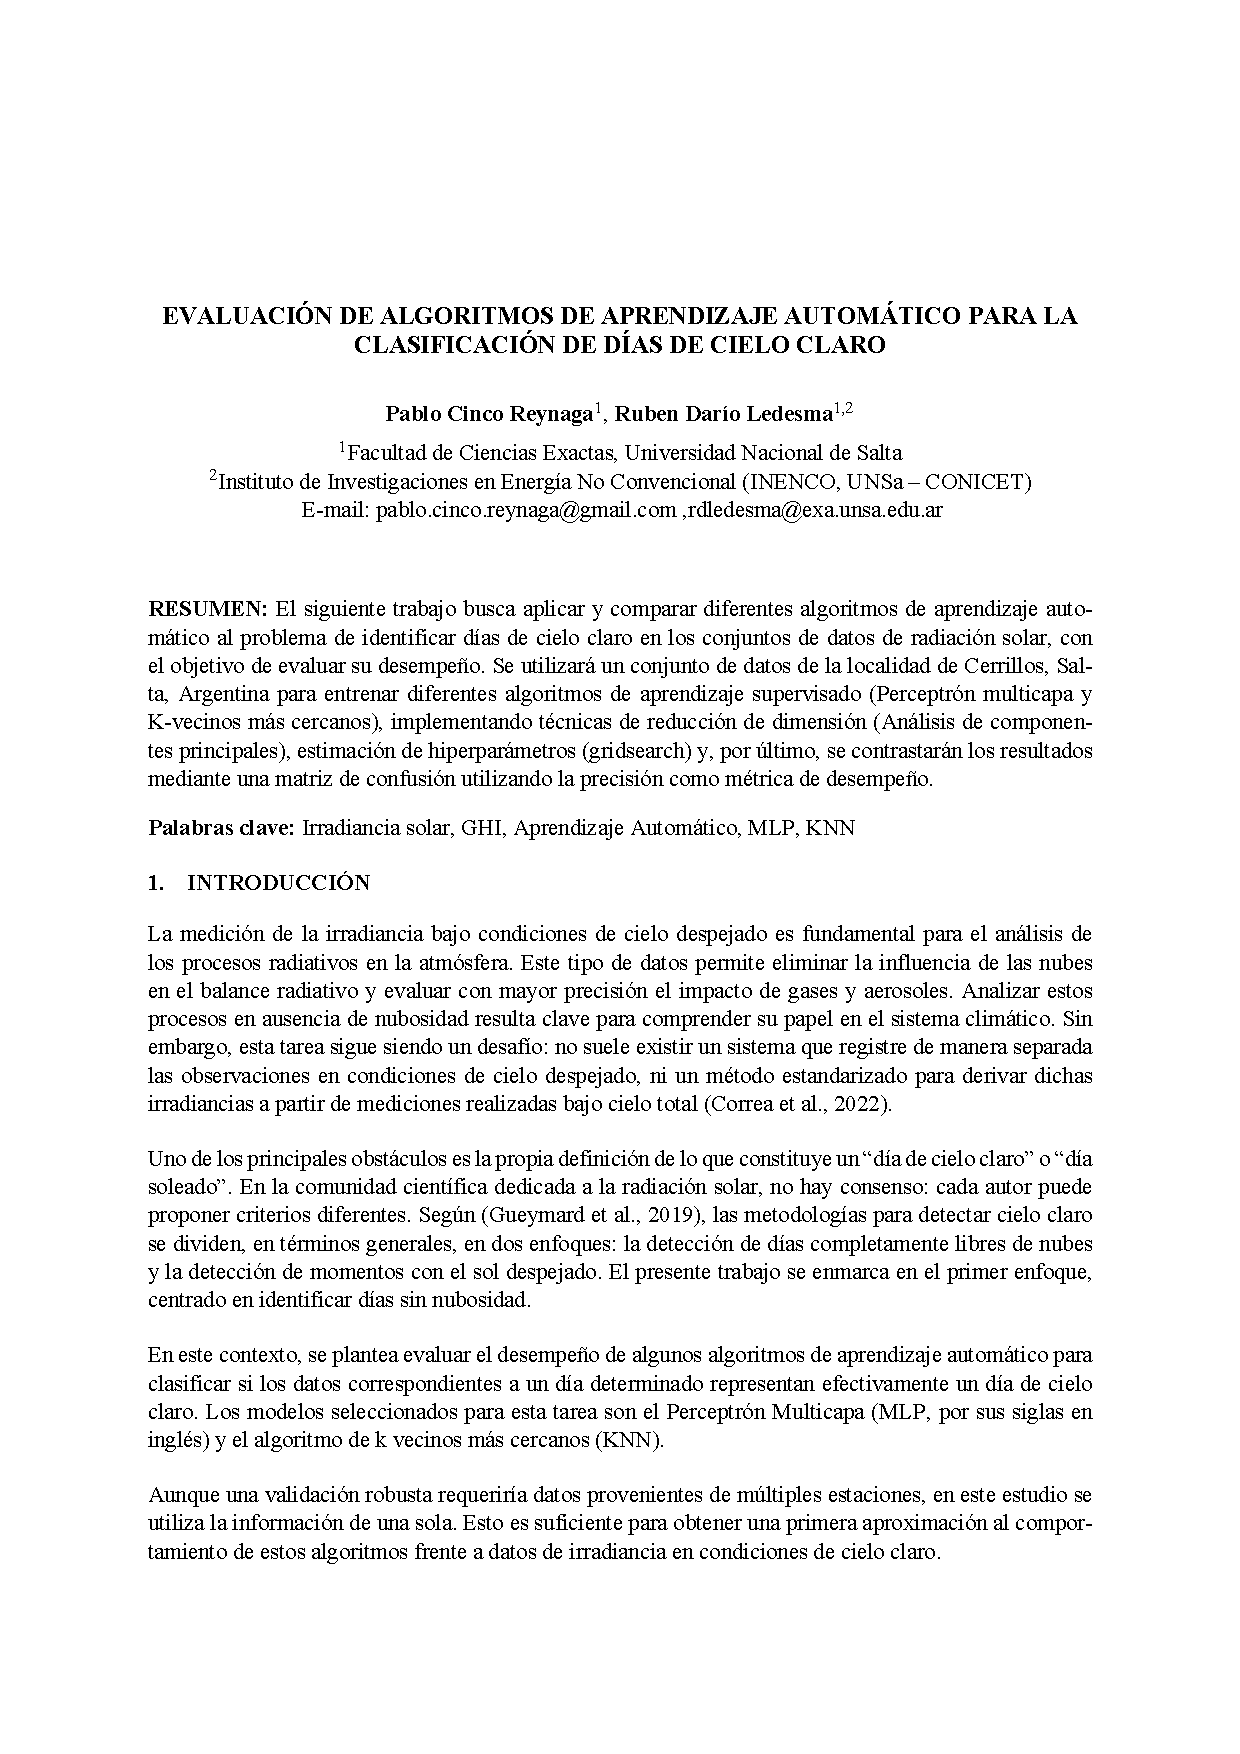
\includepdf[pages=-]{anexo_3/12_Cinco}
%DIFDELCMD < 

%DIFDELCMD <  \newpage  %%%
\DIFdelend \DIFaddbegin \addcontentsline{toc}{chapter}{\textbf{Anexo 1}} 
\lhead{Anexo 1}
\rhead{\newtitle}
\cfoot{\thepage}
\renewcommand{\headrulewidth}{1pt}
\renewcommand{\footrulewidth}{1pt}
\chapter*{Anexo 3}
\noindent En este anexo se incluyen cada una de las publicaciones que se han realizado en el transcurso de esta tesis.

\begin{itemize}
\item Salazar, G. A., Alonso-Suárez, R., Laguarda Cirigliano, A., \& Ledesma, R. D. (2022). Evaluación del proceso de adaptación al sitio aplicado a la irradiancia solar global medida en la ciudad de Salta, Argentina. Avances En Energías Renovables Y Medio Ambiente - AVERMA, 25, 353–362. 
\item Ledesma, R. D., Salazar, G. A., \& de Castro Vilela, O. (2022). Aplicación móvil como herramienta para la evaluación de modelos de irradiancia solar. En Acta de la XLIV Reunión de Trabajo de la Asociación Argentina de Energías Renovables y Ambiente (Vol. 9, pp. 186–195). ISBN 978-987-29873-1-2.

\item Ledesma, R. D., Salazar, G. A., \& de Castro Vilela, O. (2022). ARGP-V2: Un modelo práctico para la estimación de irradiancia global horizontal en condiciones de cielo claro para sitios de altura. Avances en Energías Renovables y Medio Ambiente, 26, 283–289. ISSN 2796-8111. ASADES 2022.

\item Ledesma, R., Alonso-Suárez, R., Monetta, A., Laguarda, A., Vilela, O., \& Salazar, G. (2024). Evaluación en Uruguay del producto DSR GOES-16 de irradiancia solar global horizontal. Avances En Energías Renovables Y Medio Ambiente - AVERMA, 27, 474–483.

\item Ledesma, R., Salazar, G., \& Vilela, O. (2024). Avances en la estimación de irradiancia solar en las provincias de Salta y jujuy mediante imágenes satelitales GOES-16. Avances En Energías Renovables Y Medio Ambiente - AVERMA, 27, 413–427.

\item Salazar, G., Ledesma, R. D., López Ruiz, C. ., \& de Castro Vilela, O. (2025). Análisis de desempeño de diferentes técnicas de aprendizaje automático en una adaptación al sitio de irradiancia solar global para Salta (Argentina). Avances En Energías Renovables Y Medio Ambiente - AVERMA, 28, 308–320.

\item López Ruiz, C. B., Salazar, G. A., Ledesma, R., \& Bezerra Galdino, J. J. (2025, marzo). Análisis de radiación solar difusa medida usando banda sombreadora: Caso de estudio en la ciudad de Salta. En Acta de la XLVI Reunión de Trabajo de la Asociación Argentina de Energías Renovables y Ambiente (Vol. 11, pp. 236–248). ISBN 978-987-29873-1-2.


\item Salazar, G., Ledesma, R., López Ruiz, C., \& Castro Vilela, O. (2024). Development of a solar irradiance cloud index model for Northwest Argentina using GOES-16 imagery: Comparison against reanalysis and satellite databases. En International Academy of Astronautics (Ed.), Proceedings of the International Academy of Astronautics Latin American Conference on Small Satellite Technologies and Applications (1.ª ed., pp. 191-197). International Academy of Astronautics. ISBN 978-2-917761-85-4.

\item Ledesma, R., Alonso-Suárez, R., Salazar, G., Nollas, F., \& Vilela, O. (2025). Evaluation of satellite and reanalysis models for solar irradiance estimation in Northwest Argentina. IEEE Latin America Transactions, 23(8), 706–717. https://doi.org/10.1109/TLA.2025.11072498.

\item Silvero, C. I., Forciniti, J. D., Medina, F. D., Vega Caro, M. A., Ledesma, R. D., Zossi, B. S., Mansilla, G. A., and Elias, A. G. (October 10, 2025). "Comparative Study of Solar Radiation Measurements in Tucuman, Argentina, With Reanalyses and Satellite-Based Datasets." ASME. J. Sol. Energy Eng. December 2025; 147(6): 061012.

\item Ledesma, R., Salazar, G.. (2025). Machine learning for site adaptation of satellite-derived solar irradiance in Northwestern Argentina. Journal of Computer Science and Technology, 25(2), e10. https://doi.org/10.24215/16666038.25.e10
\item Cinco Reynaga, P., \& Ledesma, R. D. (en prensa). Evaluación de algoritmos de aprendizaje automático para la clasificación de días de cielo claro. En Actas de la XLVI Reunión de Trabajo de la Asociación Argentina de Energías Renovables y Ambiente (AVERMA) (Vol. 11, pp. 236–248). ISBN 978-987-29873-1-2.
\end{itemize}
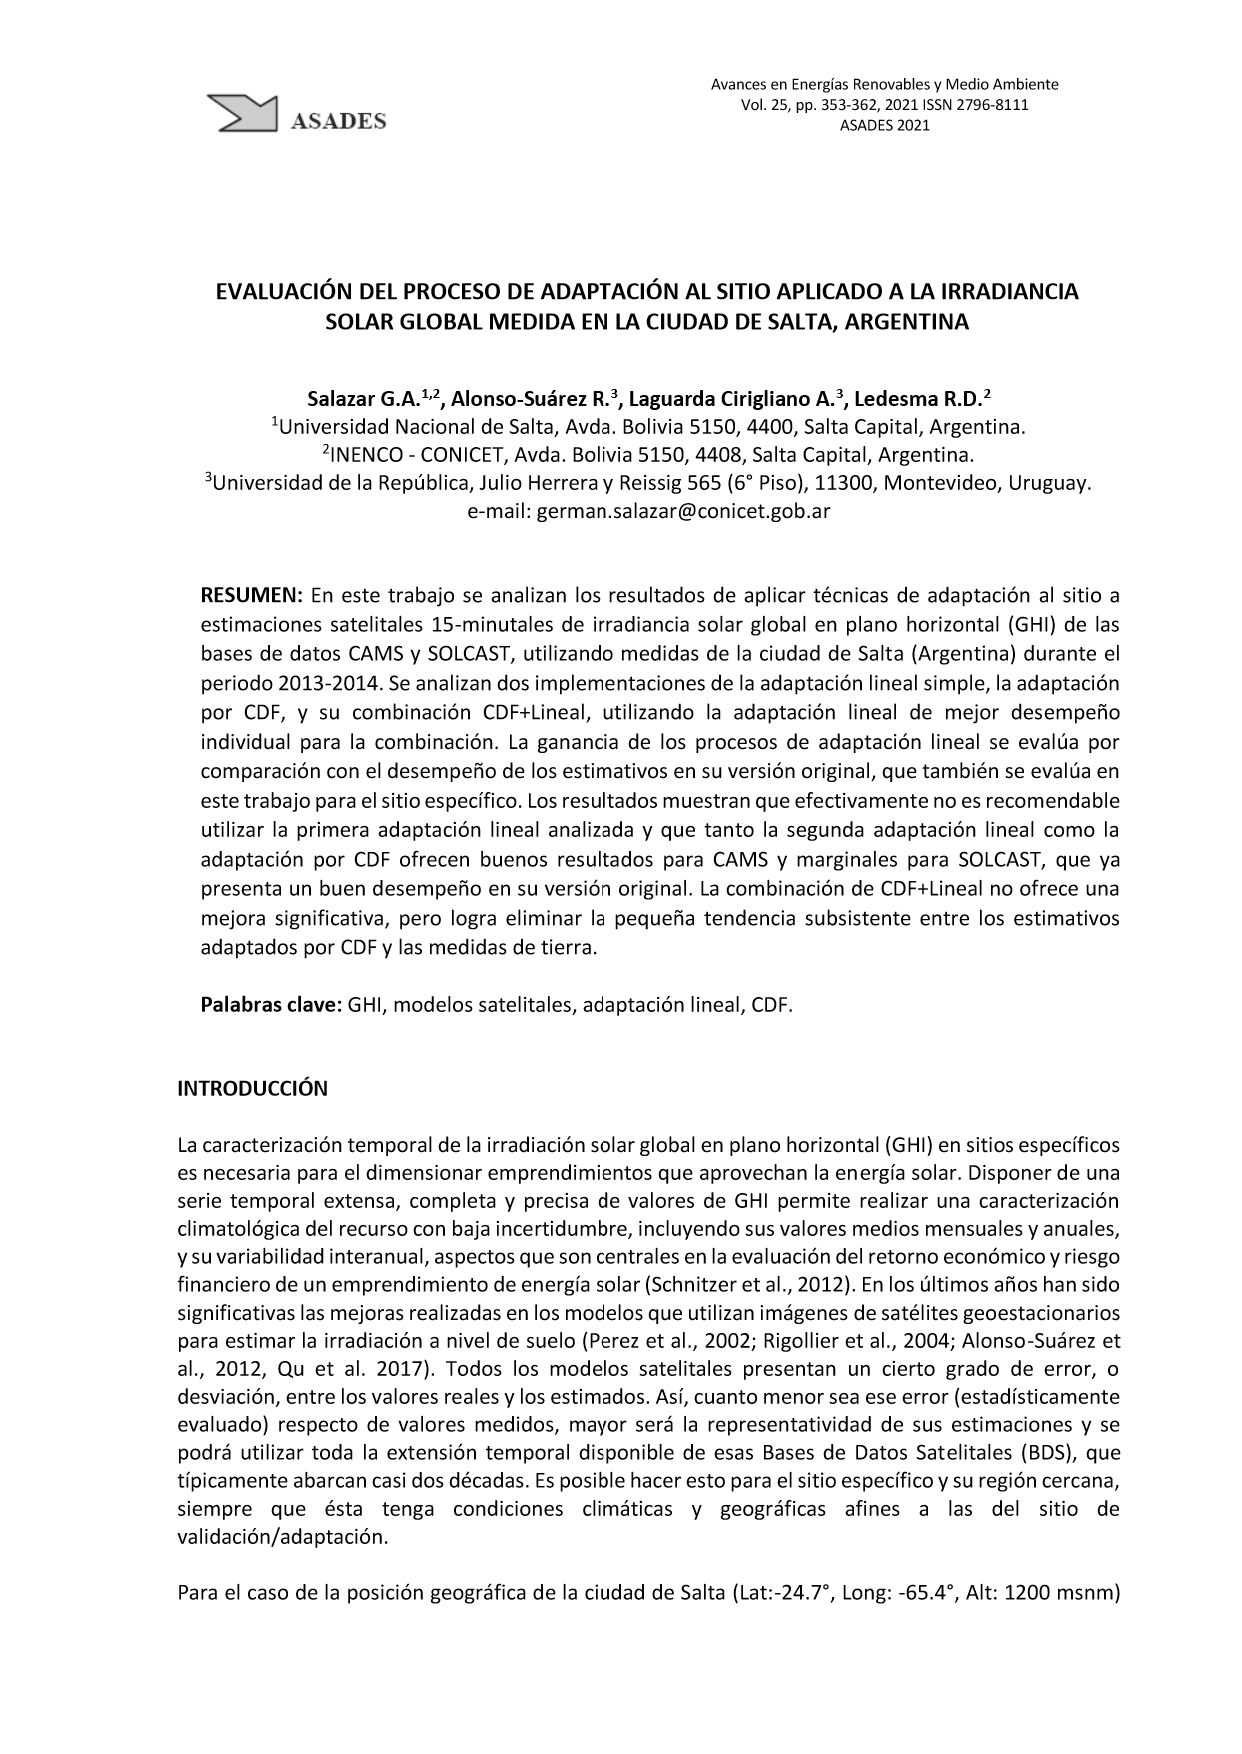
\includepdf[pages=-]{anexo_3/01_site_adaptation2}
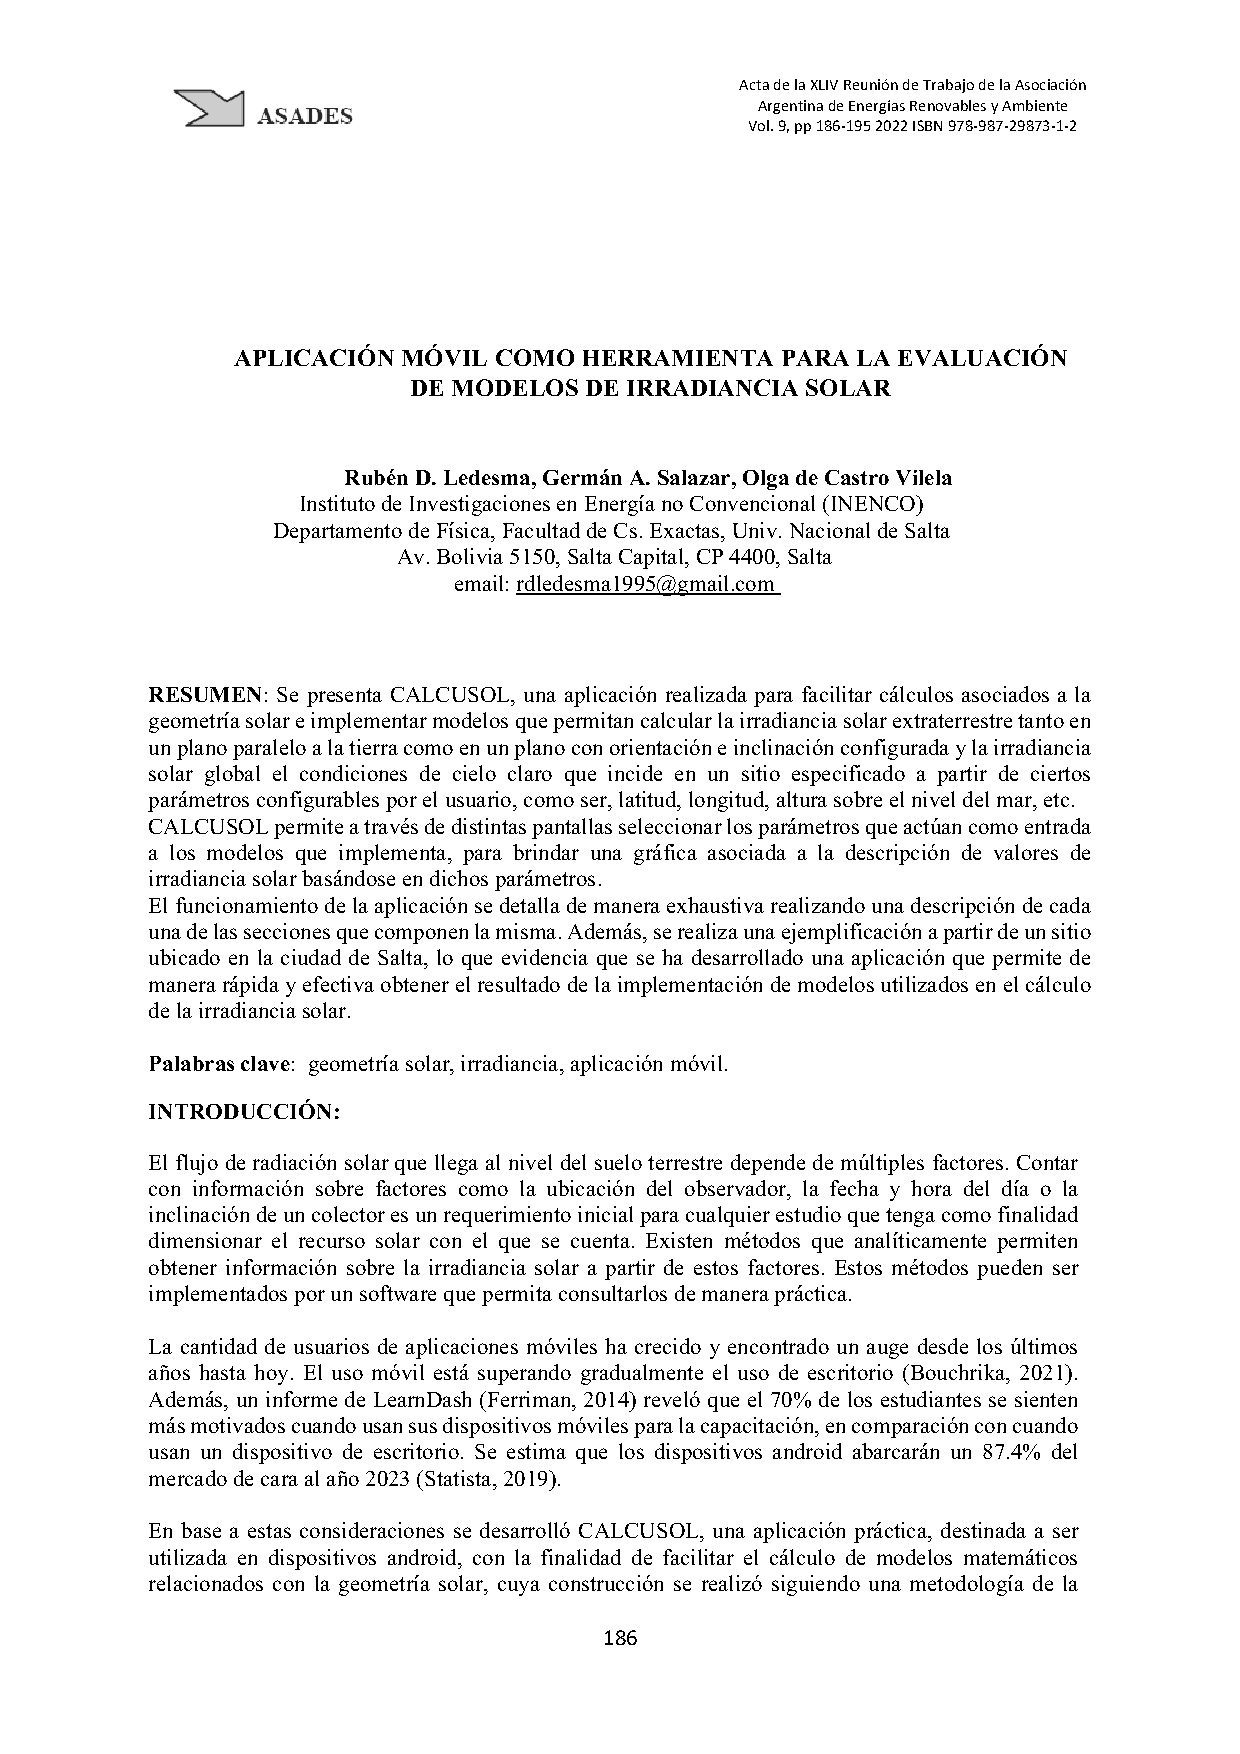
\includepdf[pages=-]{anexo_3/02_Calcusol}
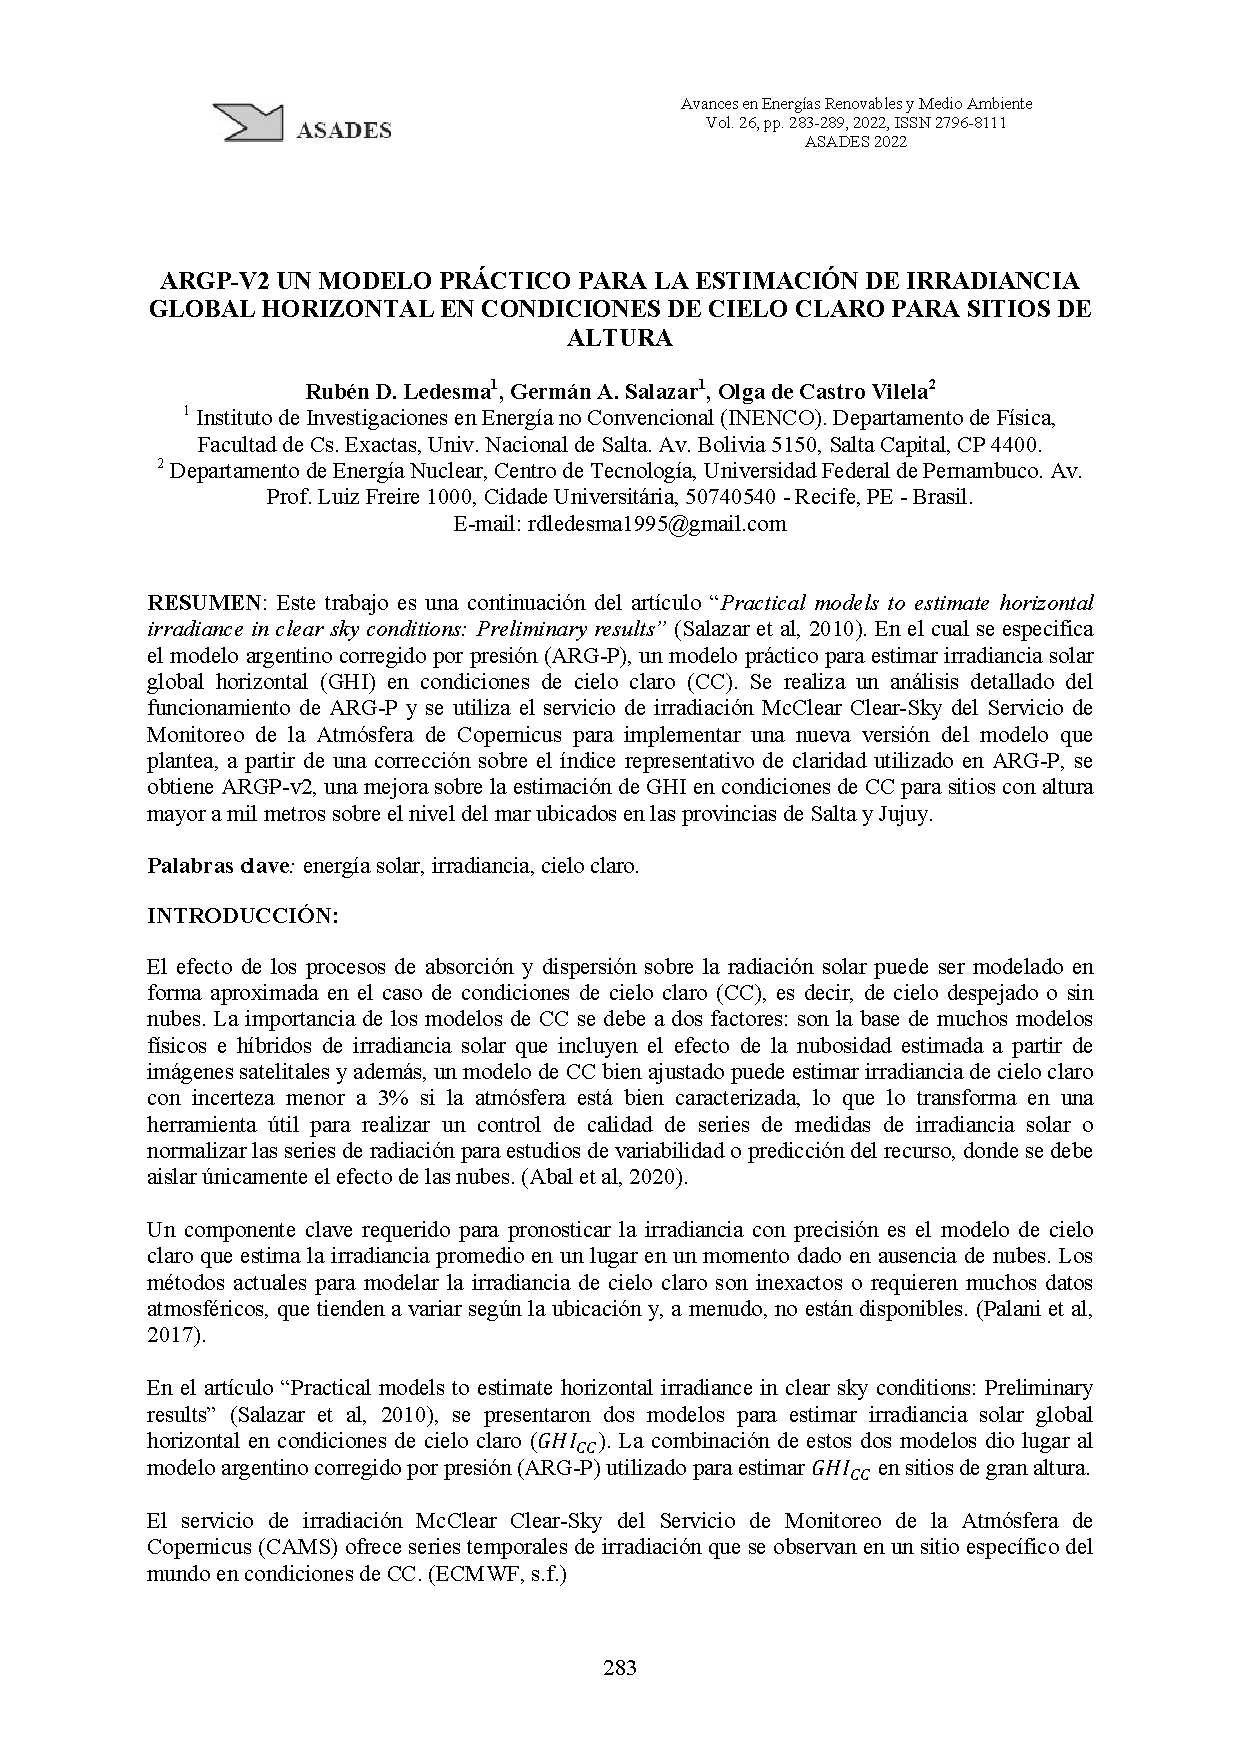
\includepdf[pages=-]{anexo_3/03_argp}
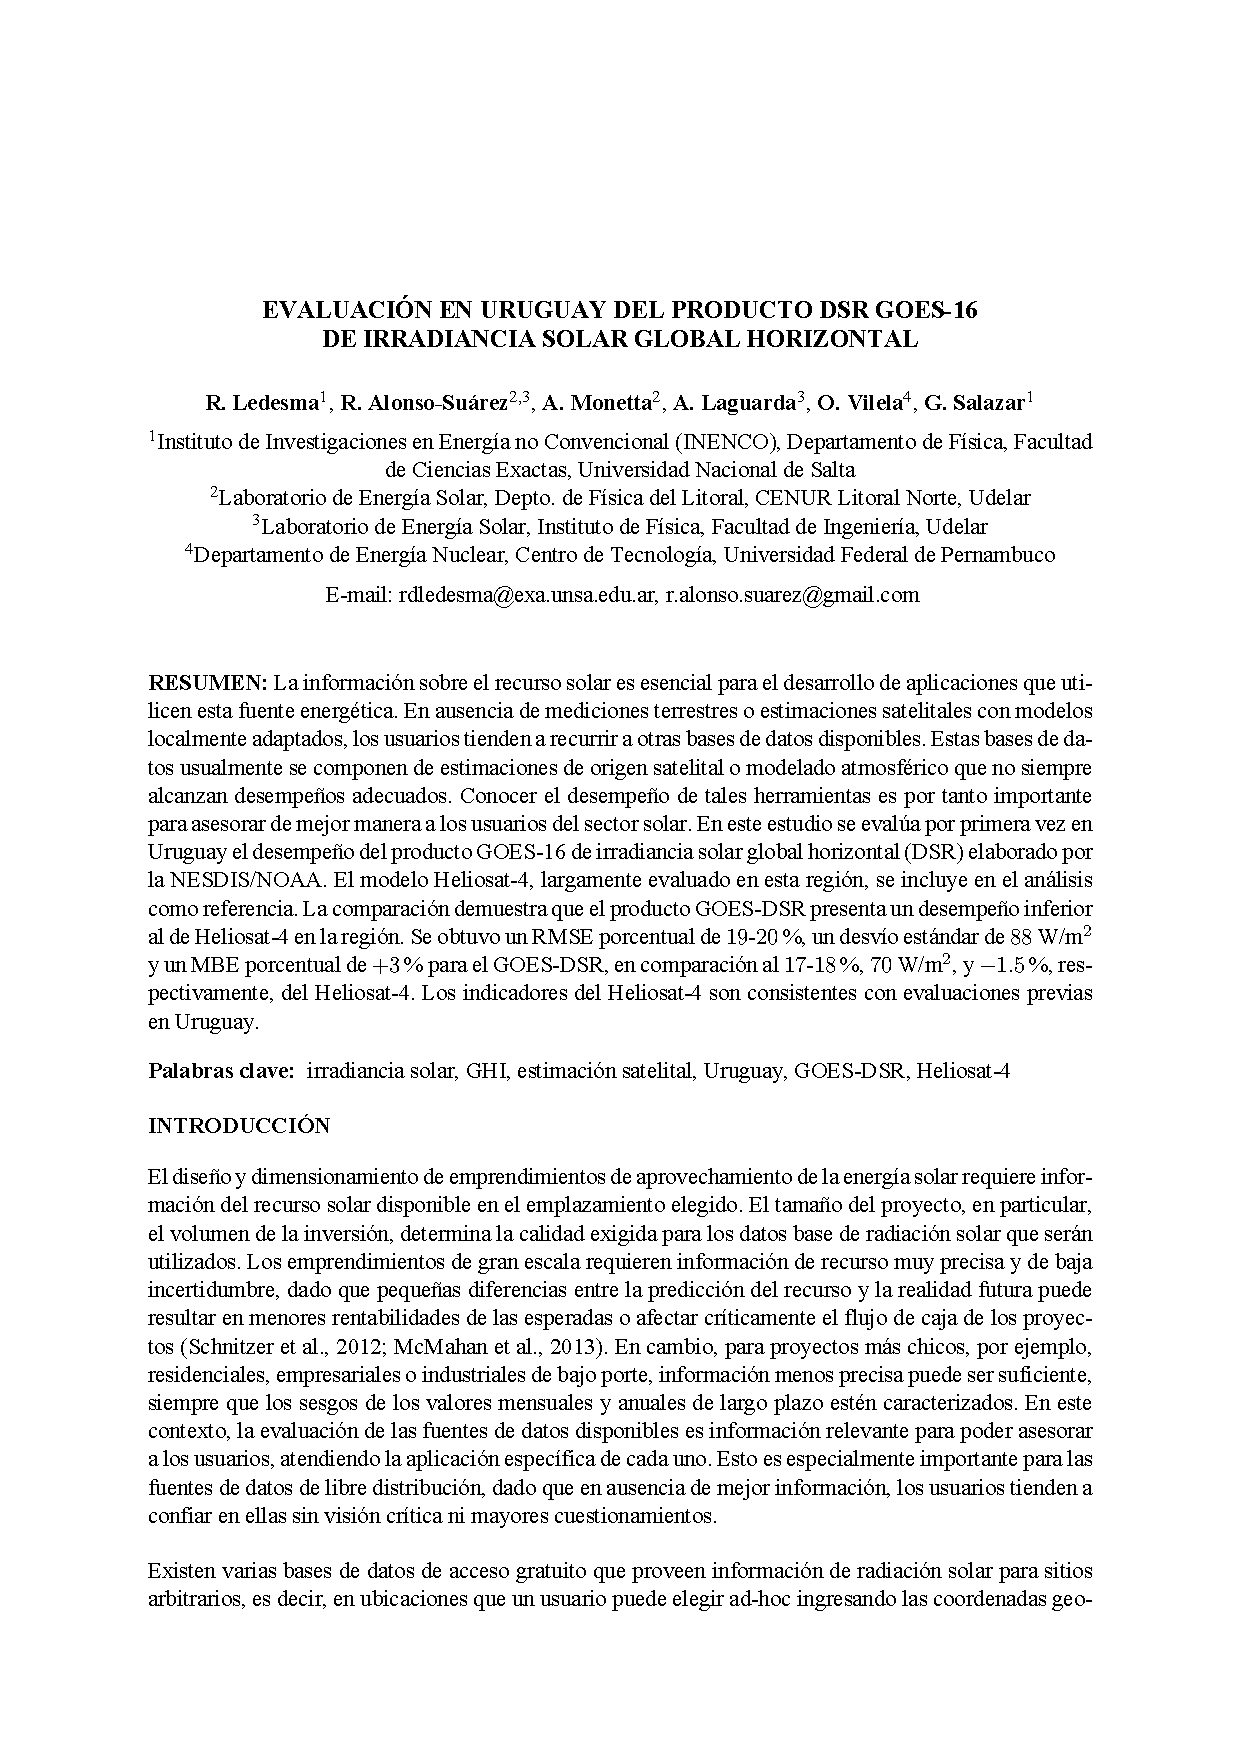
\includepdf[pages=-]{anexo_3/04_DSR}
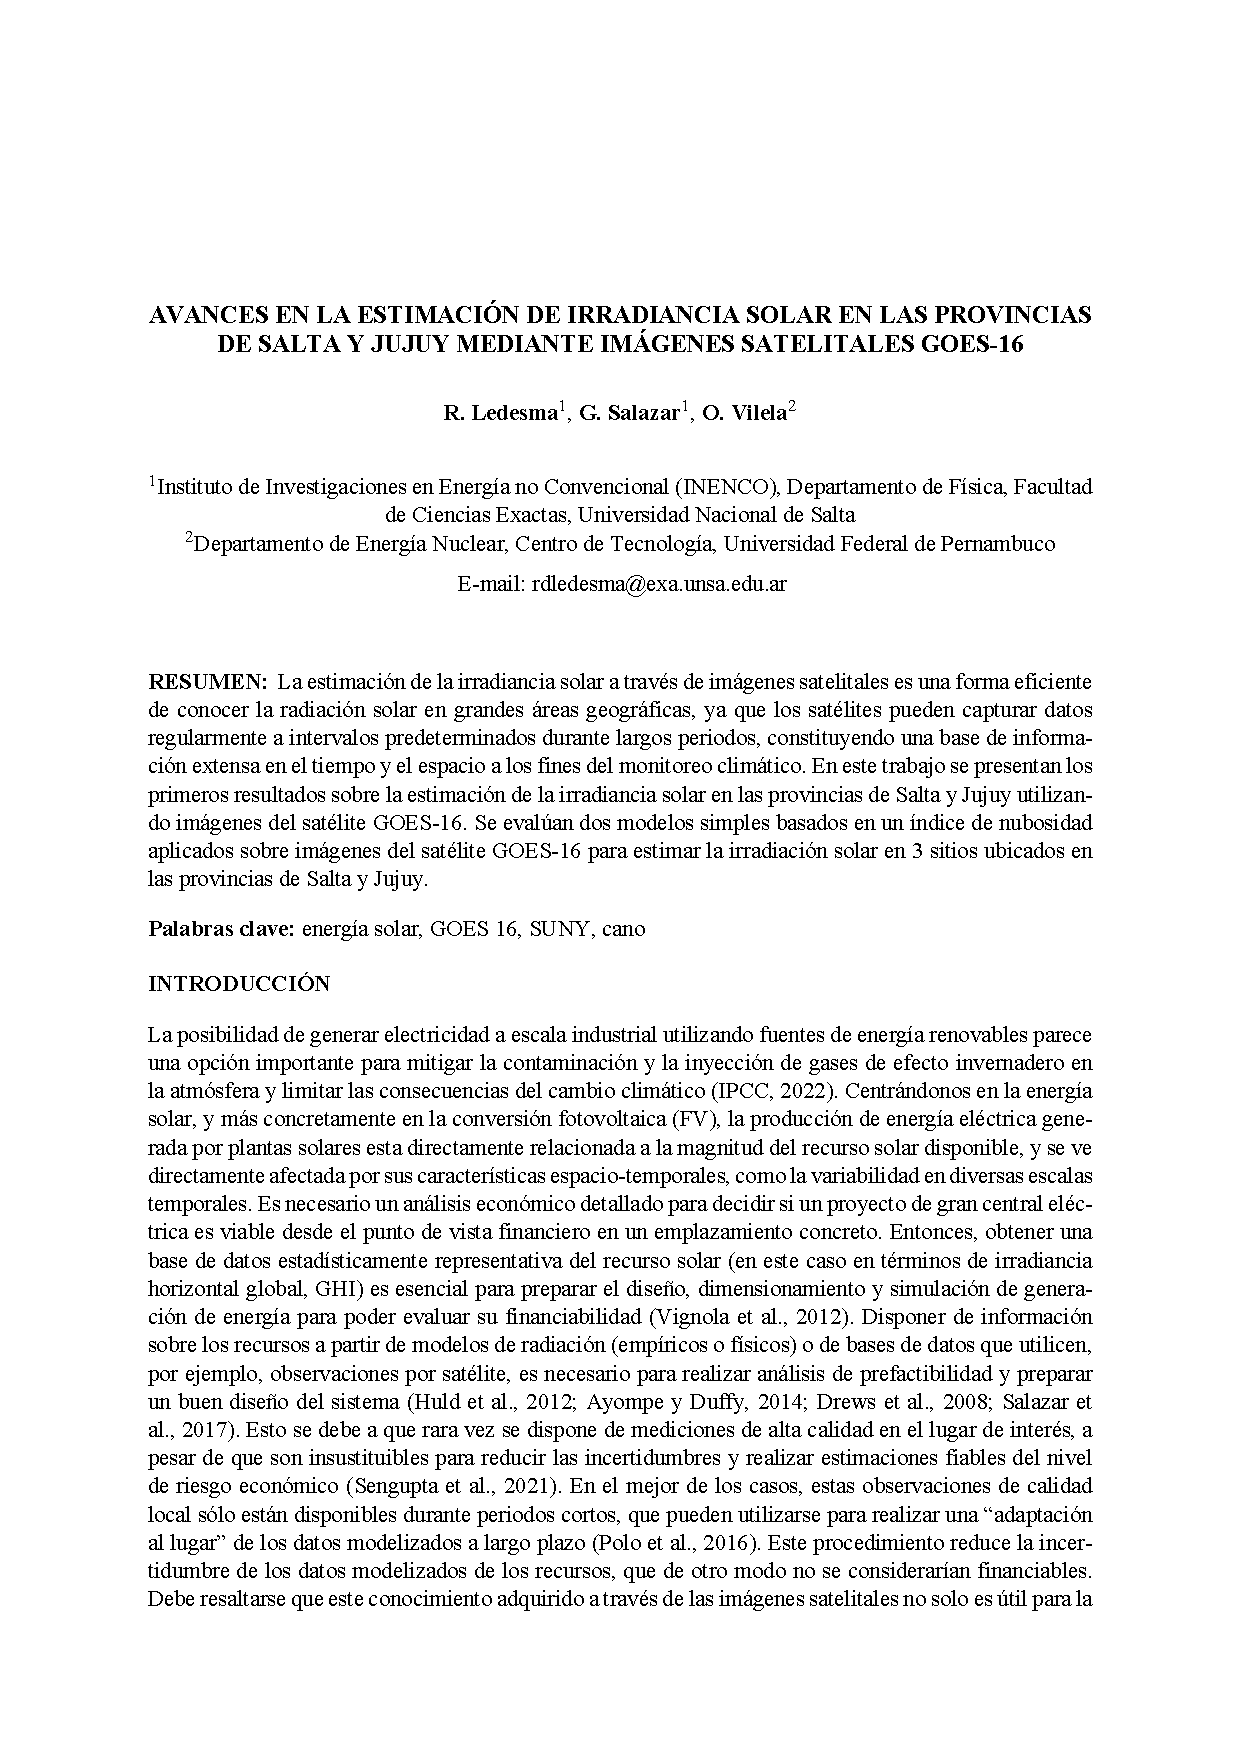
\includepdf[pages=-]{anexo_3/05_GCIM}
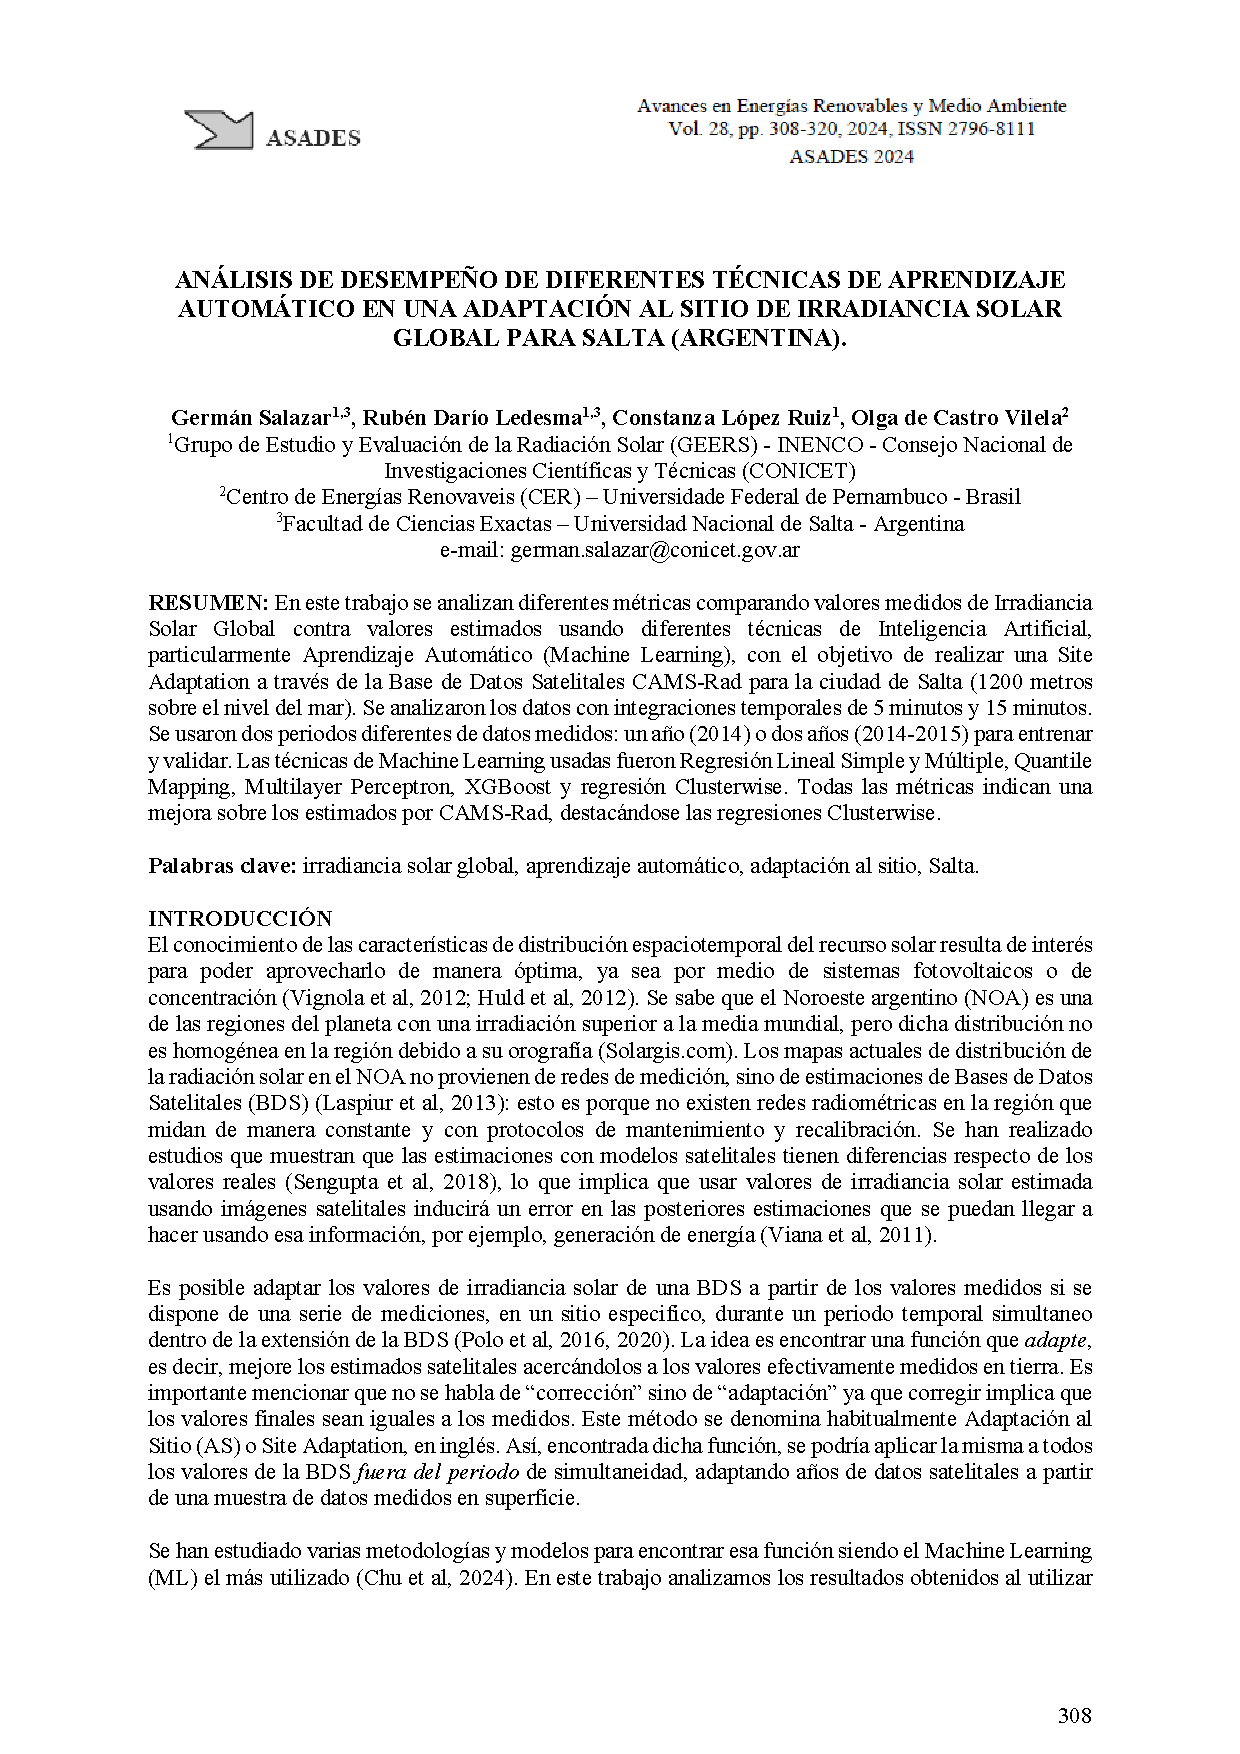
\includepdf[pages=-]{anexo_3/06_DESEMPEÑO}
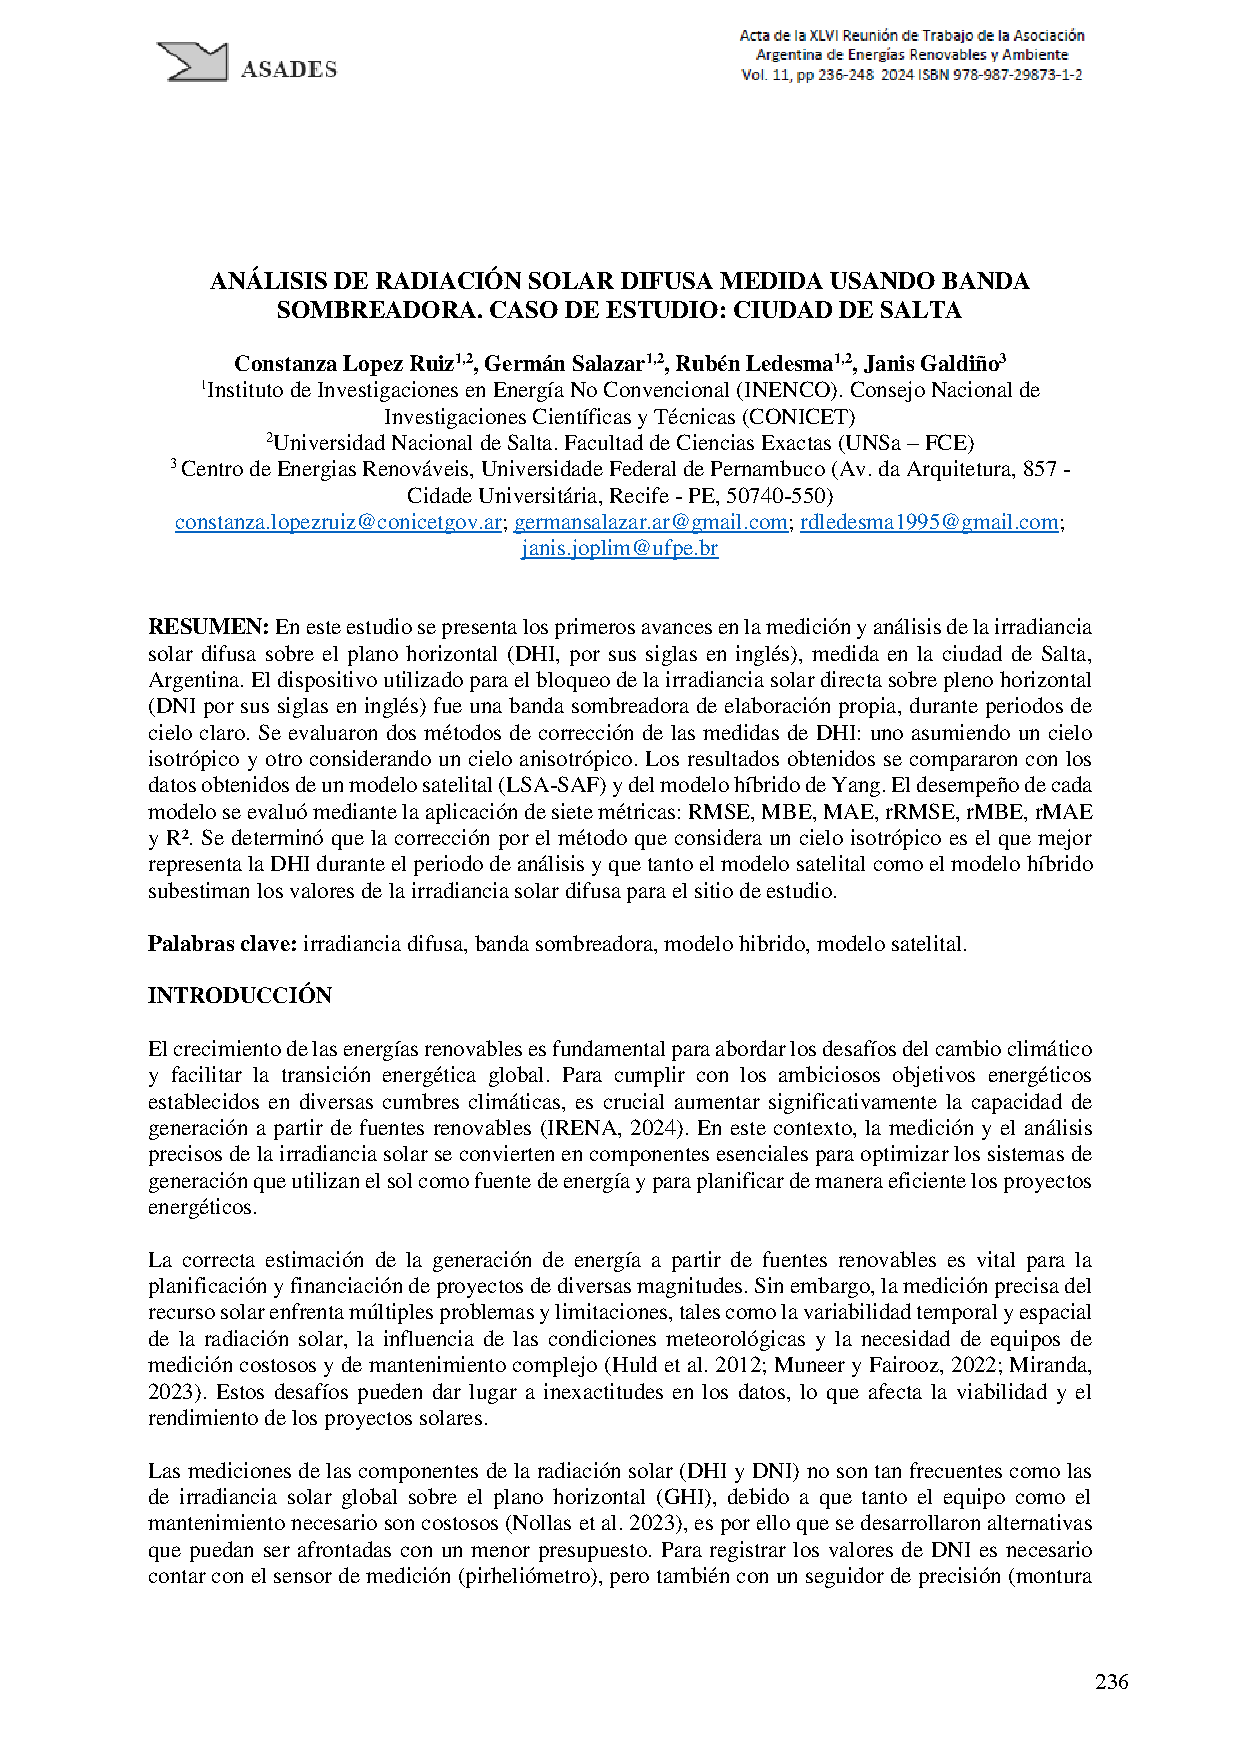
\includepdf[pages=-]{anexo_3/07_DIFUSA}

\includepdf[pages=-]{anexo_3/08_small}
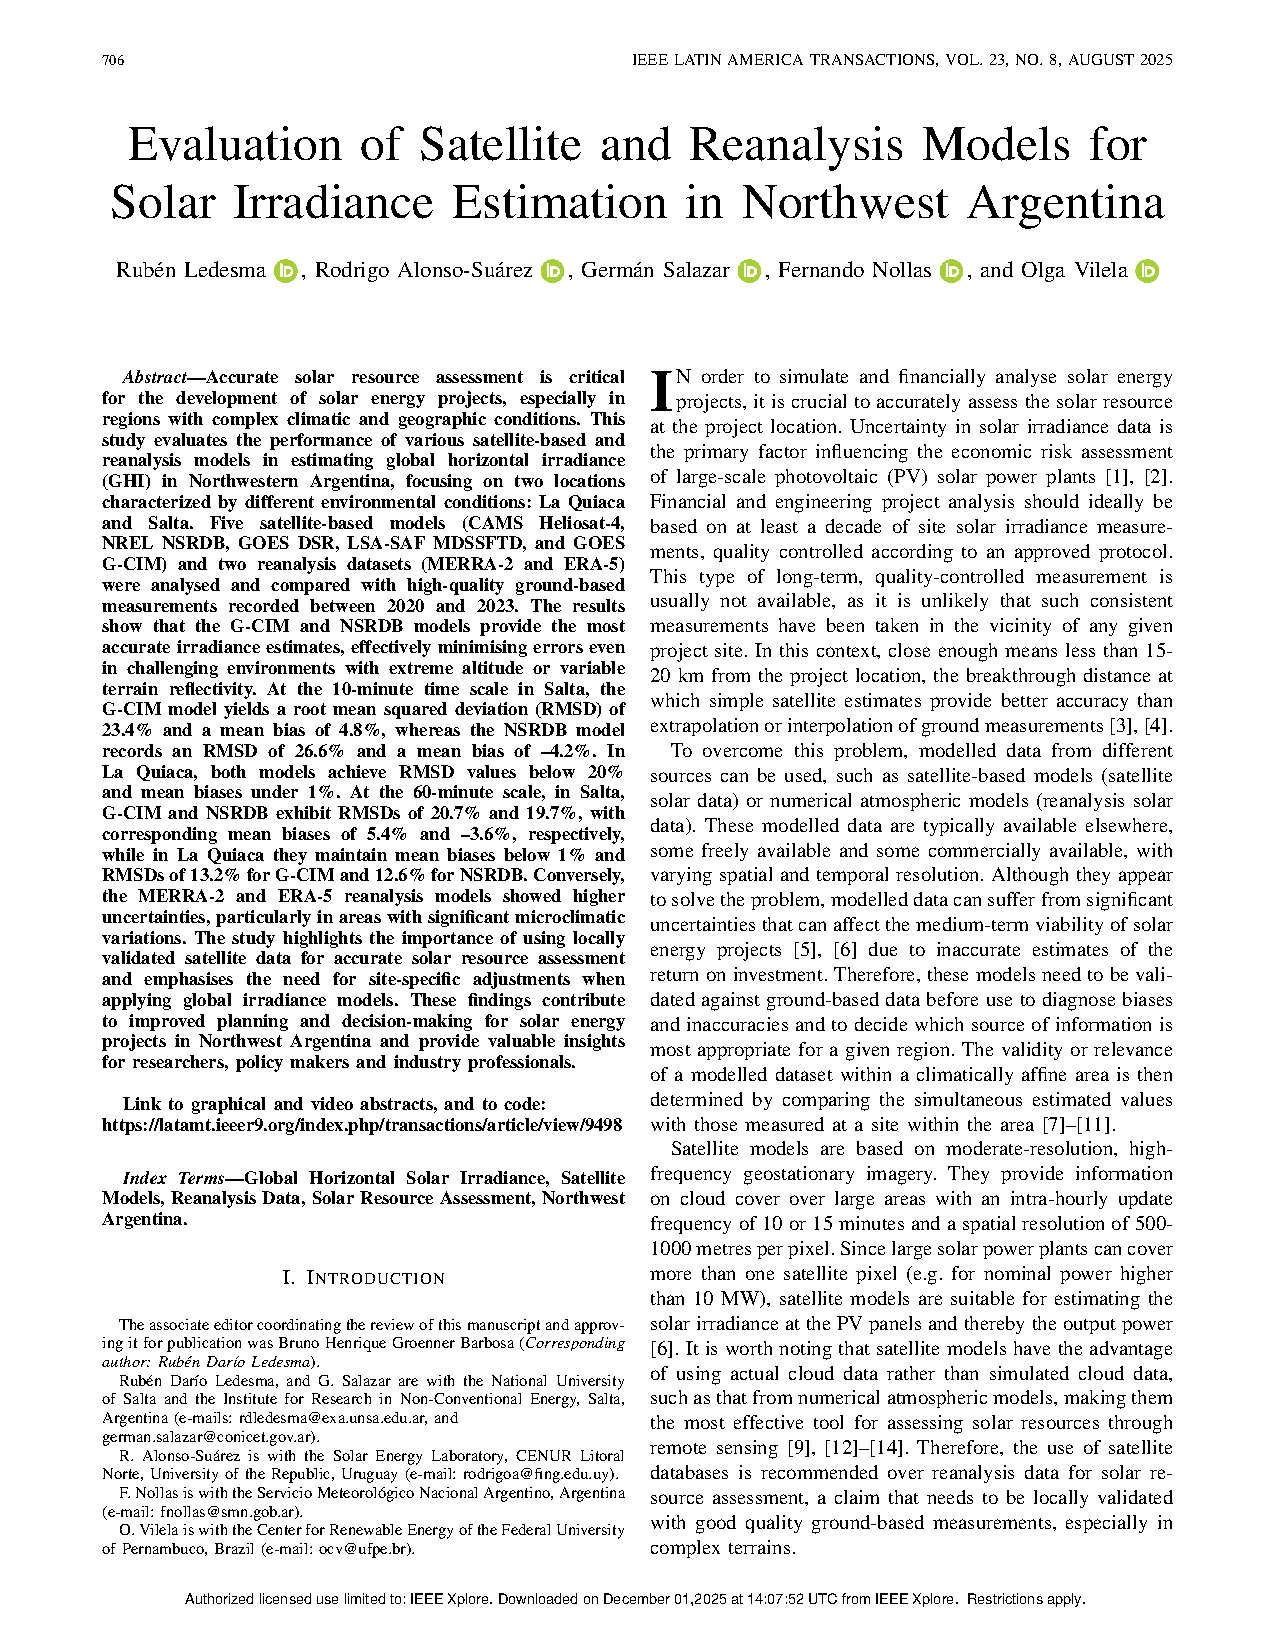
\includepdf[pages=-]{anexo_3/09_IEEE}
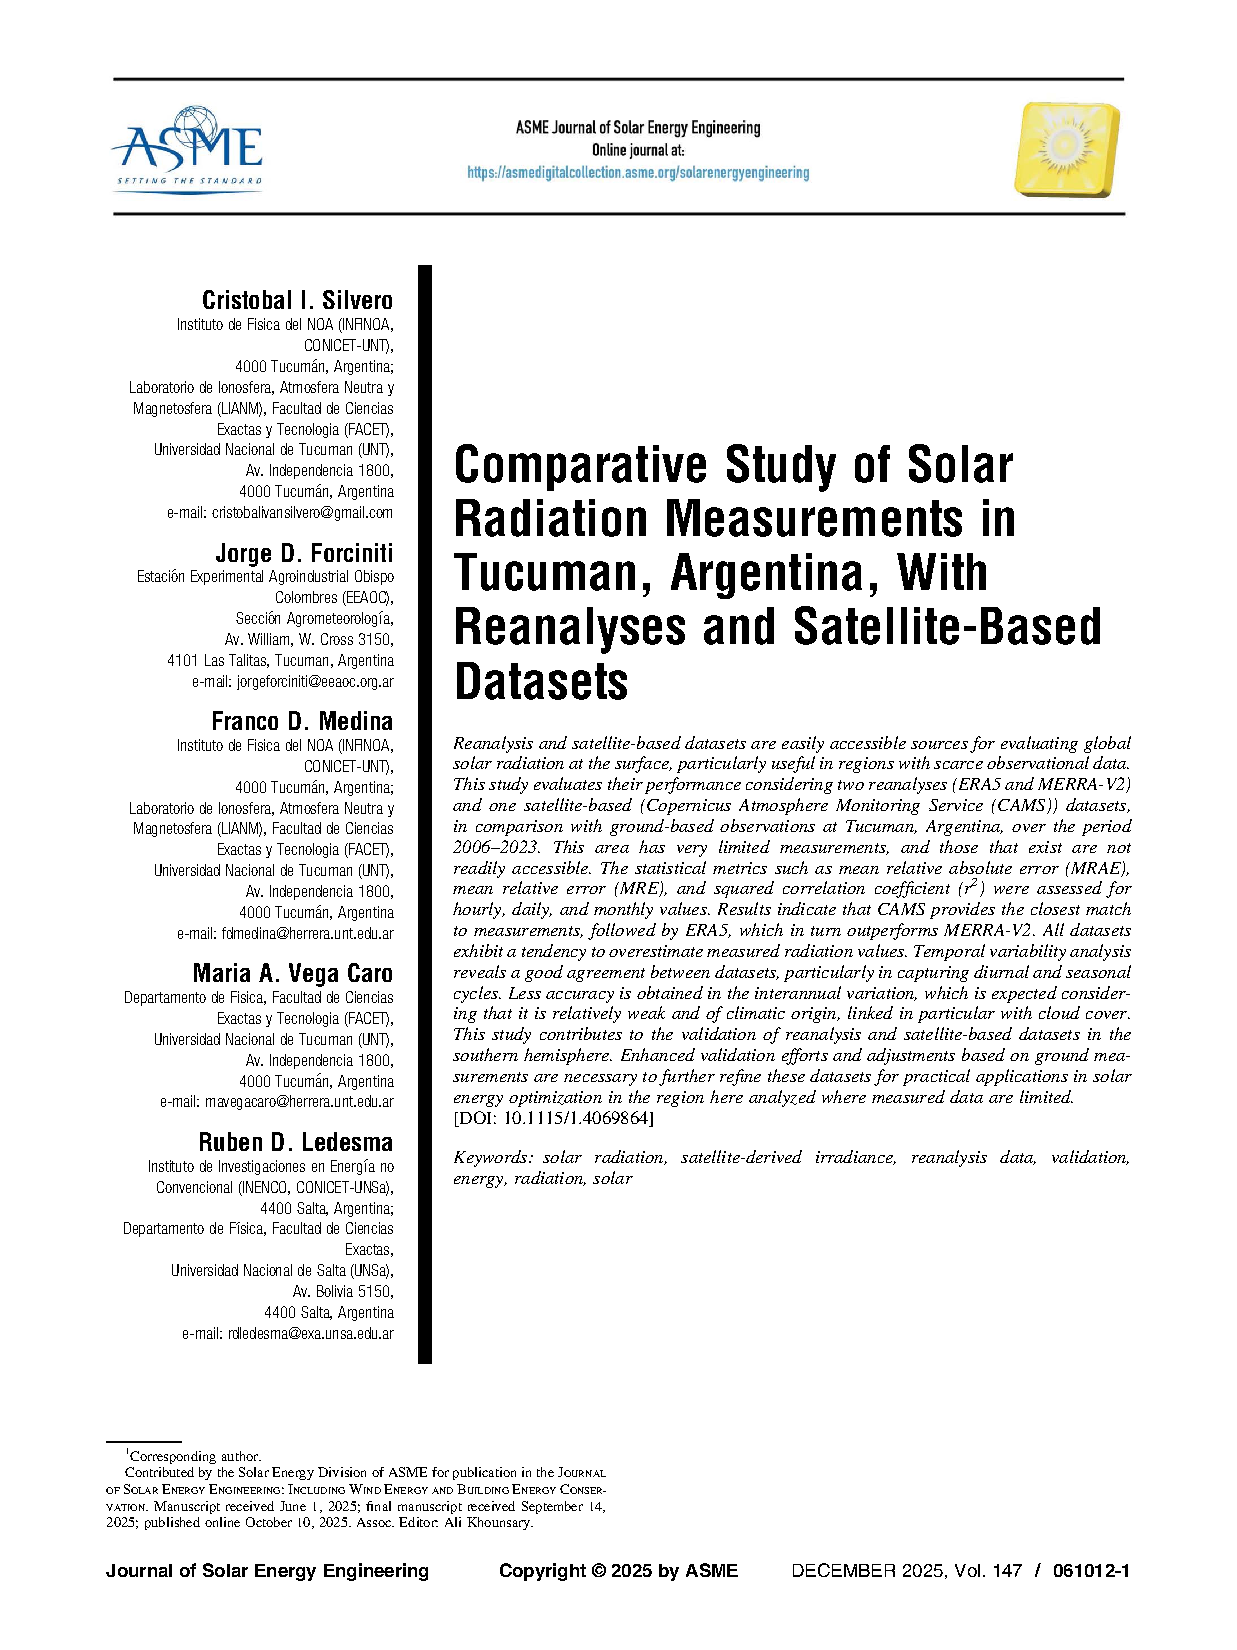
\includepdf[pages=-]{anexo_3/10_SOL}
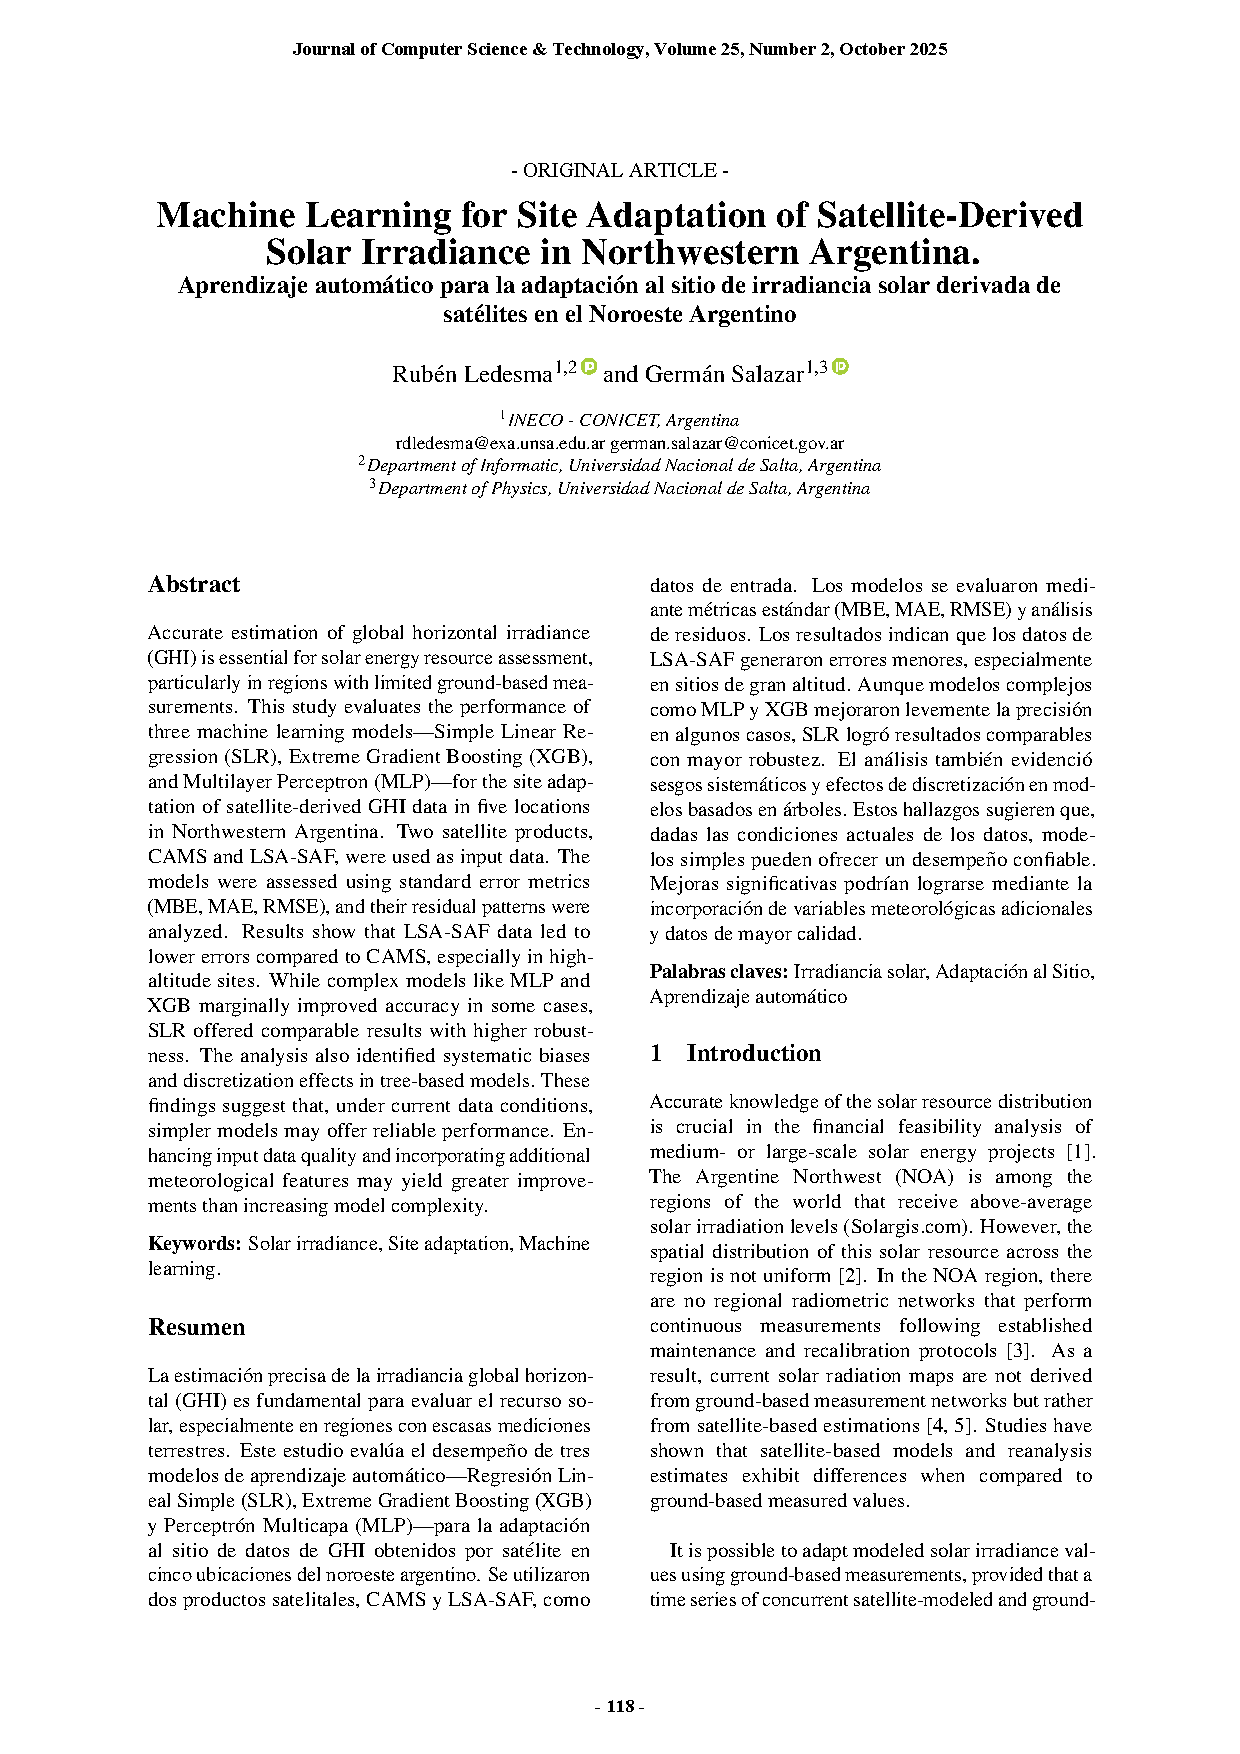
\includepdf[pages=-]{anexo_3/11_ML_JCTS}
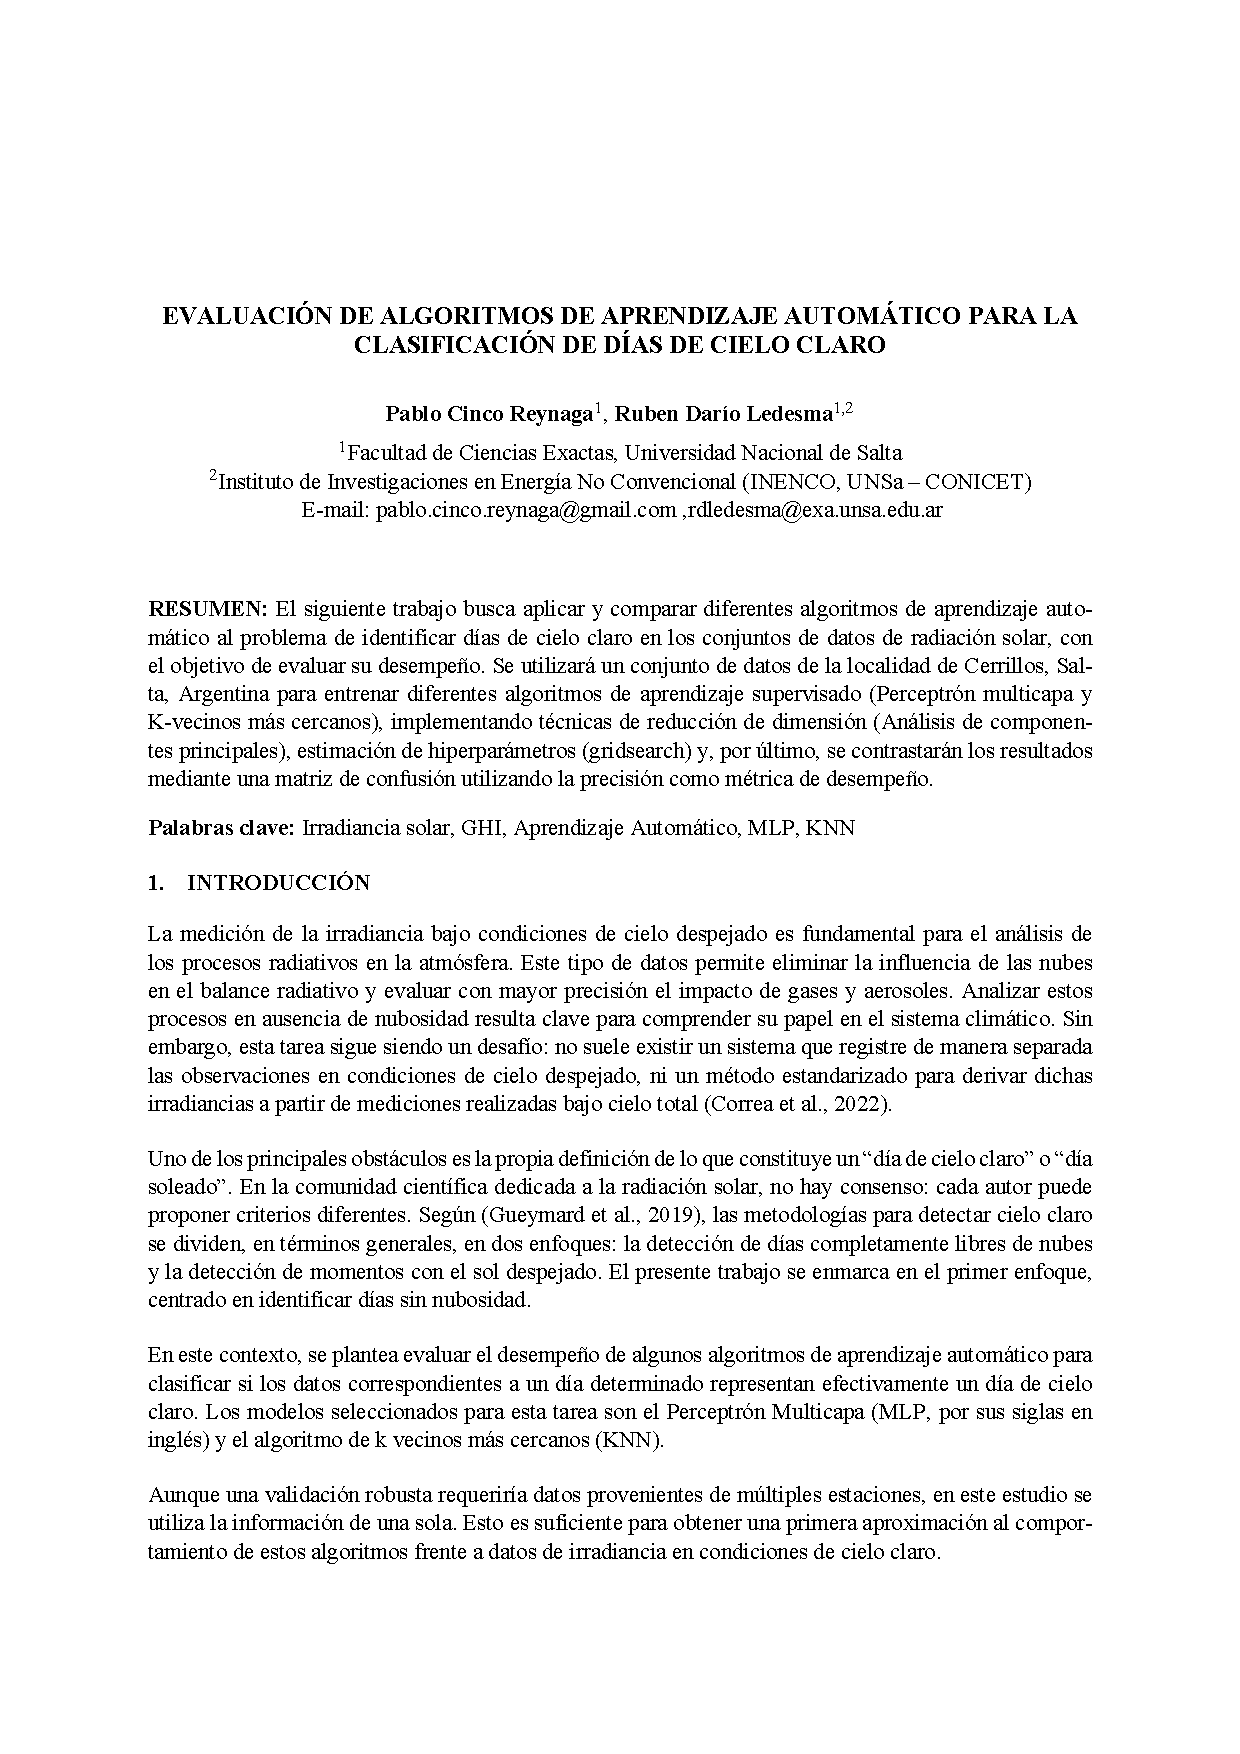
\includepdf[pages=-]{anexo_3/12_Cinco}










 \DIFaddend %Opcional: Comentar si se desea
\end{document}